\documentclass[twoside]{book}

% Packages required by doxygen
\usepackage{calc}
\usepackage{doxygen}
\usepackage{graphicx}
\usepackage[utf8]{inputenc}
\usepackage{makeidx}
\usepackage{multicol}
\usepackage{multirow}
\usepackage{fixltx2e}
\PassOptionsToPackage{warn}{textcomp}
\usepackage{textcomp}
\usepackage[nointegrals]{wasysym}
\usepackage[table]{xcolor}

% Font selection
\usepackage[T1]{fontenc}
\usepackage{mathptmx}
\usepackage[scaled=.90]{helvet}
\usepackage{courier}
\usepackage{amssymb}
\usepackage{sectsty}
\renewcommand{\familydefault}{\sfdefault}
\allsectionsfont{%
  \fontseries{bc}\selectfont%
  \color{darkgray}%
}
\renewcommand{\DoxyLabelFont}{%
  \fontseries{bc}\selectfont%
  \color{darkgray}%
}
\newcommand{\+}{\discretionary{\mbox{\scriptsize$\hookleftarrow$}}{}{}}

% Page & text layout
\usepackage{geometry}
\geometry{%
  a4paper,%
  top=2.5cm,%
  bottom=2.5cm,%
  left=2.5cm,%
  right=2.5cm%
}
\tolerance=750
\hfuzz=15pt
\hbadness=750
\setlength{\emergencystretch}{15pt}
\setlength{\parindent}{0cm}
\setlength{\parskip}{0.2cm}
\makeatletter
\renewcommand{\paragraph}{%
  \@startsection{paragraph}{4}{0ex}{-1.0ex}{1.0ex}{%
    \normalfont\normalsize\bfseries\SS@parafont%
  }%
}
\renewcommand{\subparagraph}{%
  \@startsection{subparagraph}{5}{0ex}{-1.0ex}{1.0ex}{%
    \normalfont\normalsize\bfseries\SS@subparafont%
  }%
}
\makeatother

% Headers & footers
\usepackage{fancyhdr}
\pagestyle{fancyplain}
\fancyhead[LE]{\fancyplain{}{\bfseries\thepage}}
\fancyhead[CE]{\fancyplain{}{}}
\fancyhead[RE]{\fancyplain{}{\bfseries\leftmark}}
\fancyhead[LO]{\fancyplain{}{\bfseries\rightmark}}
\fancyhead[CO]{\fancyplain{}{}}
\fancyhead[RO]{\fancyplain{}{\bfseries\thepage}}
\fancyfoot[LE]{\fancyplain{}{}}
\fancyfoot[CE]{\fancyplain{}{}}
\fancyfoot[RE]{\fancyplain{}{\bfseries\scriptsize Generated on Thu Jul 17 2014 01\+:40\+:33 for Brain\+Train by Doxygen }}
\fancyfoot[LO]{\fancyplain{}{\bfseries\scriptsize Generated on Thu Jul 17 2014 01\+:40\+:33 for Brain\+Train by Doxygen }}
\fancyfoot[CO]{\fancyplain{}{}}
\fancyfoot[RO]{\fancyplain{}{}}
\renewcommand{\footrulewidth}{0.4pt}
\renewcommand{\chaptermark}[1]{%
  \markboth{#1}{}%
}
\renewcommand{\sectionmark}[1]{%
  \markright{\thesection\ #1}%
}

% Indices & bibliography
\usepackage{natbib}
\usepackage[titles]{tocloft}
\setcounter{tocdepth}{3}
\setcounter{secnumdepth}{5}
\makeindex

% Hyperlinks (required, but should be loaded last)
\usepackage{ifpdf}
\ifpdf
  \usepackage[pdftex,pagebackref=true]{hyperref}
\else
  \usepackage[ps2pdf,pagebackref=true]{hyperref}
\fi
\hypersetup{%
  colorlinks=true,%
  linkcolor=blue,%
  citecolor=blue,%
  unicode%
}

% Custom commands
\newcommand{\clearemptydoublepage}{%
  \newpage{\pagestyle{empty}\cleardoublepage}%
}


%===== C O N T E N T S =====

\begin{document}

% Titlepage & ToC
\hypersetup{pageanchor=false,
             bookmarks=true,
             bookmarksnumbered=true,
             pdfencoding=unicode
            }
\pagenumbering{roman}
\begin{titlepage}
\vspace*{7cm}
\begin{center}%
{\Large Brain\+Train }\\
\vspace*{1cm}
{\large Generated by Doxygen 1.8.7}\\
\vspace*{0.5cm}
{\small Thu Jul 17 2014 01:40:33}\\
\end{center}
\end{titlepage}
\clearemptydoublepage
\tableofcontents
\clearemptydoublepage
\pagenumbering{arabic}
\hypersetup{pageanchor=true}

%--- Begin generated contents ---
\chapter{Brain\+Train Kurzanleitung}
\label{index}\hypertarget{index}{}For english readers\+:~\newline
 This O\+S\+G-\/\+Demo was done as part of the computer graphics I 2014 lecture of the University of Applied Sciences and Arts Hanover. This page is a short description of the project which was a requirement for passing the lecture.~\newline
 Everything written here can either also be read in the source documentation or experienced by oneself by trying out this project (look for the hidden room!)~\newline
 Everything here uses the G\+N\+U Public License. Use as you want, but give us credit =)!~\newline
 ~\newline
 Das Projekt \char`\"{}\+Brain\+Train\char`\"{} wurde im Rahmen der Vorlesung C\+G1 an der H\+S Hannover im Sommersemester 2014 erstellt.~\newline
 Beteiligt waren hierbei\+: Jonathan Spielvogel, Marcel Felix, Gleb Ostrowski, Phillip Sauer und Sebastian Huettermann.\hypertarget{index_Die}{}\section{Szene}\label{index_Die}
Ziel war es eine alte, unfertige, verfallene U-\/\+Bahn-\/\+Station zu entwerfen, in der der \char`\"{}\+Spieler\char`\"{} sich im First-\/\+Person-\/\+Shooter-\/\+Stil frei bewegen kann. Der Spieler startet am Kopf eines kleinen Niederganges, bestehend aus Treppe mit Gelaender und Rolltreppe. Direkt hinter der Startposition des Spielers befindet sich ein \char`\"{}geheimer Raum\char`\"{} (hier kann durch die Wand gelaufen werden). Der untere Teil besteht aus einem einzelnen, geschwungenen Bahnsteig (mit einem Gleis). Auf dem Bahnsteig selber befinden sich diverse Modelle, z.\+B\+: Kisten, ein altes Tickethaeuschen mit einer Folie darueber, Oelfaesser mit einer sowjetischen Flagge darueber, einem Fliesenspiegel und viele mehr. Es gibt also viel zu entdecken!

Nicht in Blender wurde hierbei folgendes erstellt\+:
\begin{DoxyItemize}
\item Die Sitzbaenke wurden in O\+S\+G modelliert, materialisiert und texturiert
\item Die Bierflaschen sowie die Vase und Blume (auf dem Tickethaeuschen) und Figuren im geheimen Raum wurden als Rotationskoerper realisiert.
\begin{DoxyItemize}
\item Die Bierflaschen wurdem zudem mit einem Partikelsystem aus Blender (zufaellig) im Raum verteilt. Die primaere Farbgebung (der \char`\"{}\+Cartoon Effekt\char`\"{} inklusive Cel Shading und Nebel) wurde hierbei ueber eigene Shader implementiert. Zudem verfuegt der Spieler ueber ein \char`\"{}\+Waffen\+H\+U\+D\char`\"{}, das eine der weiteren Kamera darstellt.
\end{DoxyItemize}
\end{DoxyItemize}\hypertarget{index_Animationen}{}\section{Animationen}\label{index_Animationen}
Mehrere Dinge sind animiert\+: Zum einen faehrt in regelmaessigen Abstaenden ein Zug das Gleis entlang. Diese Animation wurde als Animation Path in O\+S\+G realisiert. Und zum anderen weht die grosse, haengende Flagge \char`\"{}im Wind\char`\"{}. Diese Animation wurde ueber den Shader realisiert. Ebenso ueber die Shader sind die Animationen der Figuren im geheimen Raum realisiert.\hypertarget{index_Interaktive}{}\section{Elemente}\label{index_Interaktive}
In der gesamten Szene kann mit einigen Elementen interagiert werden\+:
\begin{DoxyItemize}
\item Am rechten Ende des Bahnhofs kann von einer Kiste eine \char`\"{}kaputte Portalgun\char`\"{} mittels Links-\/\+Klick aufgehoben werden. Sobald der Spieler mehr als eine Waffe traegt kann diese mittels Scrollen des Mausrades gewechselt werden.
\item Einige (drei) der herumliegenden Bierflaschen koennen getrunken werden. Hierzu muss der Spieler sich im geduckten Modus der Flasche naehern und kann diese -\/ sofern der entsprechende Texthinweis erscheint -\/ mit einem Links-\/\+Klick trinken. Hierbei handelt es sich um einen sehr starken Alkohol, der zwar schnell wirkt, seine Wirkung aber auch schnell wieder verliert.
\begin{DoxyItemize}
\item Aus Sicherheitsgruenden darf leider nicht verraten werden, um welche Flaschen es sich handelt.
\end{DoxyItemize}
\item Im Geheimraum am oberen Ende der Treppe stehen einige farbige Figuren. Naehert sich der Spieler diesen, so kann er mit einem Links-\/\+Klick u.\+a. Shader-\/\+Farben wechseln. Probieren Sie es aus!
\end{DoxyItemize}\hypertarget{index_Die}{}\section{Szene}\label{index_Die}
Die Bewegung in der Szene erfolgt im gewohnten F\+P\+S Stil. Hierbei ist sowohl eine Kollisionserkennung als auch eine \char`\"{}\+Clamp to Ground\char`\"{} Funktionalitaet implementiert (so dass der Spieler auf dem Boden laeuft). Die Tastaturbelegung ist hierbei die folgende\+:
\begin{DoxyItemize}
\item {\bfseries W} Bewegung Vorwaerts, {\bfseries S} Bewegung Rueckwaerts, {\bfseries A} Nach links bewegen (nicht drehen), {\bfseries D} Nach rechts bewegen (nicht drehen)
\item {\bfseries Maus\+:} Umschauen
\item {\bfseries Mausklick} links zur Interaktion (es erscheint immer ein Text der Interaktion \char`\"{}ankuendigt\char`\"{})
\item {\bfseries Leerstaste\+:} Springen, {\bfseries L-\/\+Shift}\+: Sprinten, {\bfseries L-\/\+Strg}\+: Gehen (langsamer gehen), {\bfseries X\+:} Ducken (um z.\+B. an Bierflaschen heranzukommen)
\item {\bfseries Mausrad} {\bfseries scrollen\+:} Wechseln der Waffe (sofern mehr als eine getragen wird) Mit der Taste {\bfseries F} kann in den Flugmodus gewechselt werden. In diesem ist die Kollisionserkennung nicht mehr aktiv. Zu der o.\+g. Steuerung kommt Folgendes hinzu\+:
\item {\bfseries Q} senkrecht nach unten fliegen, {\bfseries E} senkrecht nach oben fliegen
\end{DoxyItemize}

Weiteres\+:
\begin{DoxyItemize}
\item {\bfseries C} aktiviert/deaktiviert den Polygon-\/\+Modus
\item {\bfseries L-\/\+Shift} {\bfseries +} {\bfseries 1} wechselt durch die Shader-\/\+Modi, die normalerweise im Geheimraum umgeschaltet werden koennen
\end{DoxyItemize}\hypertarget{index_Quellenverzeichnis}{}\section{Quellenverzeichnis}\label{index_Quellenverzeichnis}
Sofern nicht anders dokumentiert (z.\+B. im Quellcode), handelt es sich bei allen Entwicklungen um Eigenentwicklungen. Insbesondere sind saemtliche Modelle Eigenentwicklungen.~\newline
 Texturen kommen hierbei geschlossen von~\newline
 \href{http://www.cgtextures.com/}{\tt http\+://www.\+cgtextures.\+com/} ~\newline
 Ausnahmen sind hierbei\+:~\newline
 U\+D\+S\+S\+R Flagge (auf den alten Oelfaessern liegend)~\newline
 \href{http://freestock.ca/soviet_union_ussr_grunge_flag_sjpg1191.jpg}{\tt http\+://freestock.\+ca/soviet\+\_\+union\+\_\+ussr\+\_\+grunge\+\_\+flag\+\_\+sjpg1191.\+jpg} ~\newline
 Zuletzt geprueft/gesehen\+: 19.\+06.\+2014~\newline
 Flagge mit Einhorn (in der Ecke haengend)~\newline
 \href{http://wallpoper.com/images/00/24/35/71/communism-soviet_00243571.jpg}{\tt http\+://wallpoper.\+com/images/00/24/35/71/communism-\/soviet\+\_\+00243571.\+jpg} ~\newline
 Zuletzt geprueft/gesehen\+: 19.\+06.\+2014~\newline

\chapter{Bug List}
\label{bug}
\hypertarget{bug}{}

\begin{DoxyRefList}
\item[\label{bug__bug000001}%
\hypertarget{bug__bug000001}{}%
Class \hyperlink{classbrtr_1_1_f_p_s_camera_manipulator}{brtr\+:\+:F\+P\+S\+Camera\+Manipulator} ]Jumping forward if there is no ground is not working~\newline

\end{DoxyRefList}
\chapter{Namespace Index}
\section{Namespace List}
Here is a list of all namespaces with brief descriptions\+:\begin{DoxyCompactList}
\item\contentsline{section}{\hyperlink{namespacebrtr}{brtr} \\*Namespace for the whole Brain\+Train Project }{\pageref{namespacebrtr}}{}
\end{DoxyCompactList}

\chapter{Hierarchical Index}
\section{Class Hierarchy}
This inheritance list is sorted roughly, but not completely, alphabetically\+:\begin{DoxyCompactList}
\item \contentsline{section}{Animation\+Creator}{\pageref{class_animation_creator}}{}
\item \contentsline{section}{brtr\+:\+:Body\+Of\+Rotation\+Function}{\pageref{structbrtr_1_1_body_of_rotation_function}}{}
\item Camera\begin{DoxyCompactList}
\item \contentsline{section}{brtr\+:\+:Weapon\+H\+U\+D}{\pageref{classbrtr_1_1_weapon_h_u_d}}{}
\end{DoxyCompactList}
\item Effect\begin{DoxyCompactList}
\item \contentsline{section}{brtr\+:\+:Cel\+Shading}{\pageref{classbrtr_1_1_cel_shading}}{}
\end{DoxyCompactList}
\item First\+Person\+Manipulator\begin{DoxyCompactList}
\item \contentsline{section}{brtr\+:\+:F\+P\+S\+Camera\+Manipulator}{\pageref{classbrtr_1_1_f_p_s_camera_manipulator}}{}
\end{DoxyCompactList}
\item G\+U\+I\+Event\+Handler\begin{DoxyCompactList}
\item \contentsline{section}{brtr\+:\+:Key\+Handler}{\pageref{classbrtr_1_1_key_handler}}{}
\item \contentsline{section}{brtr\+:\+:Weapon\+H\+U\+D\+:\+:Weapon\+Switch\+Handler}{\pageref{classbrtr_1_1_weapon_h_u_d_1_1_weapon_switch_handler}}{}
\end{DoxyCompactList}
\item Node\+Callback\begin{DoxyCompactList}
\item \contentsline{section}{brtr\+:\+:Base\+Interaction\+Callback}{\pageref{classbrtr_1_1_base_interaction_callback}}{}
\begin{DoxyCompactList}
\item \contentsline{section}{brtr\+:\+:Add\+Portal\+Gun\+Interaction\+Callback}{\pageref{classbrtr_1_1_add_portal_gun_interaction_callback}}{}
\item \contentsline{section}{brtr\+:\+:Drunken\+Interaction\+Callback}{\pageref{classbrtr_1_1_drunken_interaction_callback}}{}
\item \contentsline{section}{brtr\+:\+:Program\+Switcher\+Callback}{\pageref{classbrtr_1_1_program_switcher_callback}}{}
\item \contentsline{section}{brtr\+:\+:Toon\+Tex\+Switcher\+Callback}{\pageref{classbrtr_1_1_toon_tex_switcher_callback}}{}
\end{DoxyCompactList}
\item \contentsline{section}{brtr\+:\+:Train\+Switcher\+Callback}{\pageref{classbrtr_1_1_train_switcher_callback}}{}
\end{DoxyCompactList}
\item Node\+Visitor\begin{DoxyCompactList}
\item \contentsline{section}{brtr\+:\+:Add\+Interaction\+Callback\+To\+Drawable\+Visitor}{\pageref{classbrtr_1_1_add_interaction_callback_to_drawable_visitor}}{}
\item \contentsline{section}{brtr\+:\+:Geometry\+Placer\+Visitor}{\pageref{classbrtr_1_1_geometry_placer_visitor}}{}
\item \contentsline{section}{brtr\+:\+:Modify\+Material\+Visitor}{\pageref{classbrtr_1_1_modify_material_visitor}}{}
\end{DoxyCompactList}
\item Position\+Attitude\+Transform\begin{DoxyCompactList}
\item \contentsline{section}{brtr\+:\+:Bench}{\pageref{classbrtr_1_1_bench}}{}
\item \contentsline{section}{brtr\+:\+:Control\+Room}{\pageref{classbrtr_1_1_control_room}}{}
\end{DoxyCompactList}
\item \contentsline{section}{brtr\+:\+:Rendering\+Pipeline}{\pageref{structbrtr_1_1_rendering_pipeline}}{}
\item Technique\begin{DoxyCompactList}
\item \contentsline{section}{brtr\+:\+:Cel\+Shading\+Technique}{\pageref{classbrtr_1_1_cel_shading_technique}}{}
\end{DoxyCompactList}
\end{DoxyCompactList}

\chapter{Class Index}
\section{Class List}
Here are the classes, structs, unions and interfaces with brief descriptions\+:\begin{DoxyCompactList}
\item\contentsline{section}{\hyperlink{classbrtr_1_1_add_interaction_callback_to_drawable_visitor}{brtr\+::\+Add\+Interaction\+Callback\+To\+Drawable\+Visitor} \\*Node\+Visitor for batch replacing all User\+Data\+Container of all Drawables }{\pageref{classbrtr_1_1_add_interaction_callback_to_drawable_visitor}}{}
\item\contentsline{section}{\hyperlink{classbrtr_1_1_add_portal_gun_interaction_callback}{brtr\+::\+Add\+Portal\+Gun\+Interaction\+Callback} \\*Interaction\+Callback for adding the portal gun to the players inventar }{\pageref{classbrtr_1_1_add_portal_gun_interaction_callback}}{}
\item\contentsline{section}{\hyperlink{class_animation_creator}{Animation\+Creator} }{\pageref{class_animation_creator}}{}
\item\contentsline{section}{\hyperlink{classbrtr_1_1_base_interaction_callback}{brtr\+::\+Base\+Interaction\+Callback} \\*This is the Template\+Class for Interaction\+Callbacks }{\pageref{classbrtr_1_1_base_interaction_callback}}{}
\item\contentsline{section}{\hyperlink{classbrtr_1_1_bench}{brtr\+::\+Bench} \\*\hyperlink{classbrtr_1_1_bench}{Bench} class, creates a bench Object }{\pageref{classbrtr_1_1_bench}}{}
\item\contentsline{section}{\hyperlink{structbrtr_1_1_body_of_rotation_function}{brtr\+::\+Body\+Of\+Rotation\+Function} \\*Struct holding the function, which calculates the radius in dependece of the height. lambda (double)-\/$>$double func, int end, Body\+Of\+Rotation\+Function$\ast$ next\+Func if one wish to have more then one function then the end value and next\+Func pointer must be set accordingly the end+1 is the beginning x of the next function }{\pageref{structbrtr_1_1_body_of_rotation_function}}{}
\item\contentsline{section}{\hyperlink{classbrtr_1_1_cel_shading}{brtr\+::\+Cel\+Shading} \\*Cel\+Sading Effect, every child of this node will get the effect }{\pageref{classbrtr_1_1_cel_shading}}{}
\item\contentsline{section}{\hyperlink{classbrtr_1_1_cel_shading_technique}{brtr\+::\+Cel\+Shading\+Technique} \\*The Technique for the cel-\/shading effect }{\pageref{classbrtr_1_1_cel_shading_technique}}{}
\item\contentsline{section}{\hyperlink{classbrtr_1_1_control_room}{brtr\+::\+Control\+Room} \\*Control Room Class, derived from Position\+Attitude\+Transform, set ups the whole room as its own children }{\pageref{classbrtr_1_1_control_room}}{}
\item\contentsline{section}{\hyperlink{classbrtr_1_1_drunken_interaction_callback}{brtr\+::\+Drunken\+Interaction\+Callback} \\*Callback for the drunk effect }{\pageref{classbrtr_1_1_drunken_interaction_callback}}{}
\item\contentsline{section}{\hyperlink{classbrtr_1_1_f_p_s_camera_manipulator}{brtr\+::\+F\+P\+S\+Camera\+Manipulator} \\*A F\+P\+S style Camera\+Manipulator with ground clamping and intersection }{\pageref{classbrtr_1_1_f_p_s_camera_manipulator}}{}
\item\contentsline{section}{\hyperlink{classbrtr_1_1_geometry_placer_visitor}{brtr\+::\+Geometry\+Placer\+Visitor} \\*Node\+Visitor for batch replacing all Geometry in all visited Geodes }{\pageref{classbrtr_1_1_geometry_placer_visitor}}{}
\item\contentsline{section}{\hyperlink{classbrtr_1_1_key_handler}{brtr\+::\+Key\+Handler} \\*Key Handler Class, handles all of our Key\+Functions, which do not belong to camera control (this are handled by \hyperlink{classbrtr_1_1_f_p_s_camera_manipulator}{F\+P\+S\+Camera\+Manipulator}) }{\pageref{classbrtr_1_1_key_handler}}{}
\item\contentsline{section}{\hyperlink{classbrtr_1_1_modify_material_visitor}{brtr\+::\+Modify\+Material\+Visitor} \\*Visitor for altering the material attributes, mainly used for objects craeted with blender }{\pageref{classbrtr_1_1_modify_material_visitor}}{}
\item\contentsline{section}{\hyperlink{classbrtr_1_1_program_switcher_callback}{brtr\+::\+Program\+Switcher\+Callback} \\*Callback for switching the postprocess programs }{\pageref{classbrtr_1_1_program_switcher_callback}}{}
\item\contentsline{section}{\hyperlink{structbrtr_1_1_rendering_pipeline}{brtr\+::\+Rendering\+Pipeline} \\*Struct holding the camera for the multi-\/rendering passes. Also holds the program vector for the post process pass. pass0\+Color, pass0depth, pass\+Post\+Process, program array, count program\+Array The program vector is used by the \hyperlink{classbrtr_1_1_key_handler}{Key\+Handler} and the Interaction\+Items for changing the postprocess programs }{\pageref{structbrtr_1_1_rendering_pipeline}}{}
\item\contentsline{section}{\hyperlink{classbrtr_1_1_toon_tex_switcher_callback}{brtr\+::\+Toon\+Tex\+Switcher\+Callback} \\*Callback for switching the Toon\+Textures }{\pageref{classbrtr_1_1_toon_tex_switcher_callback}}{}
\item\contentsline{section}{\hyperlink{classbrtr_1_1_train_switcher_callback}{brtr\+::\+Train\+Switcher\+Callback} \\*Callback for switching the \char`\"{}trains\char`\"{} }{\pageref{classbrtr_1_1_train_switcher_callback}}{}
\item\contentsline{section}{\hyperlink{classbrtr_1_1_weapon_h_u_d}{brtr\+::\+Weapon\+H\+U\+D} \\*\hyperlink{classbrtr_1_1_weapon_h_u_d}{Weapon\+H\+U\+D} class, provides the functions to add a H\+U\+D camera to the scene }{\pageref{classbrtr_1_1_weapon_h_u_d}}{}
\item\contentsline{section}{\hyperlink{classbrtr_1_1_weapon_h_u_d_1_1_weapon_switch_handler}{brtr\+::\+Weapon\+H\+U\+D\+::\+Weapon\+Switch\+Handler} \\*Event\+Handler for Weapon\+Switching }{\pageref{classbrtr_1_1_weapon_h_u_d_1_1_weapon_switch_handler}}{}
\end{DoxyCompactList}

\chapter{File Index}
\section{File List}
Here is a list of all files with brief descriptions\+:\begin{DoxyCompactList}
\item\contentsline{section}{Animation/\hyperlink{_animation_creater_8cpp}{Animation\+Creater.\+cpp} }{\pageref{_animation_creater_8cpp}}{}
\item\contentsline{section}{Callbacks/\hyperlink{_add_portal_gun_interaction_callback_8cpp}{Add\+Portal\+Gun\+Interaction\+Callback.\+cpp} }{\pageref{_add_portal_gun_interaction_callback_8cpp}}{}
\item\contentsline{section}{Callbacks/\hyperlink{_base_interaction_callback_8cpp}{Base\+Interaction\+Callback.\+cpp} }{\pageref{_base_interaction_callback_8cpp}}{}
\item\contentsline{section}{Callbacks/\hyperlink{_drunken_interaction_callback_8cpp}{Drunken\+Interaction\+Callback.\+cpp} }{\pageref{_drunken_interaction_callback_8cpp}}{}
\item\contentsline{section}{Callbacks/\hyperlink{_program_switcher_callback_8cpp}{Program\+Switcher\+Callback.\+cpp} }{\pageref{_program_switcher_callback_8cpp}}{}
\item\contentsline{section}{Callbacks/\hyperlink{_toon_tex_switcher_callback_8cpp}{Toon\+Tex\+Switcher\+Callback.\+cpp} }{\pageref{_toon_tex_switcher_callback_8cpp}}{}
\item\contentsline{section}{Callbacks/\hyperlink{_train_switcher_callback_8cpp}{Train\+Switcher\+Callback.\+cpp} }{\pageref{_train_switcher_callback_8cpp}}{}
\item\contentsline{section}{Camera/\hyperlink{_f_p_s_camera_manipulator_8cpp}{F\+P\+S\+Camera\+Manipulator.\+cpp} }{\pageref{_f_p_s_camera_manipulator_8cpp}}{}
\item\contentsline{section}{Camera/\hyperlink{_weapon_h_u_d_8cpp}{Weapon\+H\+U\+D.\+cpp} }{\pageref{_weapon_h_u_d_8cpp}}{}
\item\contentsline{section}{G\+U\+I/\hyperlink{_key_handler_8cpp}{Key\+Handler.\+cpp} }{\pageref{_key_handler_8cpp}}{}
\item\contentsline{section}{header/\hyperlink{_add_interaction_callback_to_drawable_visitor_8h}{Add\+Interaction\+Callback\+To\+Drawable\+Visitor.\+h} }{\pageref{_add_interaction_callback_to_drawable_visitor_8h}}{}
\item\contentsline{section}{header/\hyperlink{_add_portal_gun_interaction_callback_8h}{Add\+Portal\+Gun\+Interaction\+Callback.\+h} }{\pageref{_add_portal_gun_interaction_callback_8h}}{}
\item\contentsline{section}{header/\hyperlink{_animation_creater_8h}{Animation\+Creater.\+h} }{\pageref{_animation_creater_8h}}{}
\item\contentsline{section}{header/\hyperlink{_base_interaction_callback_8h}{Base\+Interaction\+Callback.\+h} }{\pageref{_base_interaction_callback_8h}}{}
\item\contentsline{section}{header/\hyperlink{_bench_8h}{Bench.\+h} }{\pageref{_bench_8h}}{}
\item\contentsline{section}{header/\hyperlink{_cel_shading_8h}{Cel\+Shading.\+h} }{\pageref{_cel_shading_8h}}{}
\item\contentsline{section}{header/\hyperlink{_control_room_8h}{Control\+Room.\+h} }{\pageref{_control_room_8h}}{}
\item\contentsline{section}{header/\hyperlink{_drunken_interaction_callback_8h}{Drunken\+Interaction\+Callback.\+h} }{\pageref{_drunken_interaction_callback_8h}}{}
\item\contentsline{section}{header/\hyperlink{_f_p_s_camera_manipulator_8h}{F\+P\+S\+Camera\+Manipulator.\+h} }{\pageref{_f_p_s_camera_manipulator_8h}}{}
\item\contentsline{section}{header/\hyperlink{_geometry_placer_visitor_8h}{Geometry\+Placer\+Visitor.\+h} }{\pageref{_geometry_placer_visitor_8h}}{}
\item\contentsline{section}{header/\hyperlink{_key_handler_8h}{Key\+Handler.\+h} }{\pageref{_key_handler_8h}}{}
\item\contentsline{section}{header/\hyperlink{_modify_material_visitor_8h}{Modify\+Material\+Visitor.\+h} }{\pageref{_modify_material_visitor_8h}}{}
\item\contentsline{section}{header/\hyperlink{_program_switcher_callback_8h}{Program\+Switcher\+Callback.\+h} }{\pageref{_program_switcher_callback_8h}}{}
\item\contentsline{section}{header/\hyperlink{_toon_tex_switcher_callback_8h}{Toon\+Tex\+Switcher\+Callback.\+h} }{\pageref{_toon_tex_switcher_callback_8h}}{}
\item\contentsline{section}{header/\hyperlink{_train_switcher_callback_8h}{Train\+Switcher\+Callback.\+h} }{\pageref{_train_switcher_callback_8h}}{}
\item\contentsline{section}{header/\hyperlink{_util_functions_8h}{Util\+Functions.\+h} }{\pageref{_util_functions_8h}}{}
\item\contentsline{section}{header/\hyperlink{_weapon_h_u_d_8h}{Weapon\+H\+U\+D.\+h} }{\pageref{_weapon_h_u_d_8h}}{}
\item\contentsline{section}{Main/\hyperlink{_main_8cpp}{Main.\+cpp} \\*Main file which loads and set ups everything }{\pageref{_main_8cpp}}{}
\item\contentsline{section}{Objects/\hyperlink{_bench_8cpp}{Bench.\+cpp} }{\pageref{_bench_8cpp}}{}
\item\contentsline{section}{Objects/\hyperlink{_control_room_8cpp}{Control\+Room.\+cpp} }{\pageref{_control_room_8cpp}}{}
\item\contentsline{section}{Shader/\hyperlink{_cel_shading_8cpp}{Cel\+Shading.\+cpp} }{\pageref{_cel_shading_8cpp}}{}
\item\contentsline{section}{Util/\hyperlink{_add_interaction_callback_to_drawable_visitor_8cpp}{Add\+Interaction\+Callback\+To\+Drawable\+Visitor.\+cpp} }{\pageref{_add_interaction_callback_to_drawable_visitor_8cpp}}{}
\item\contentsline{section}{Util/\hyperlink{_geometry_placer_visitor_8cpp}{Geometry\+Placer\+Visitor.\+cpp} }{\pageref{_geometry_placer_visitor_8cpp}}{}
\item\contentsline{section}{Util/\hyperlink{_modify_material_visitor_8cpp}{Modify\+Material\+Visitor.\+cpp} }{\pageref{_modify_material_visitor_8cpp}}{}
\item\contentsline{section}{Util/\hyperlink{_util_functions_8cpp}{Util\+Functions.\+cpp} }{\pageref{_util_functions_8cpp}}{}
\end{DoxyCompactList}

\chapter{Namespace Documentation}
\hypertarget{namespacebrtr}{\section{brtr Namespace Reference}
\label{namespacebrtr}\index{brtr@{brtr}}
}


Namespace for the whole Brain\+Train Project.  


\subsection*{Classes}
\begin{DoxyCompactItemize}
\item 
class \hyperlink{classbrtr_1_1_add_interaction_callback_to_drawable_visitor}{Add\+Interaction\+Callback\+To\+Drawable\+Visitor}
\begin{DoxyCompactList}\small\item\em Node\+Visitor for batch replacing all User\+Data\+Container of all Drawables. \end{DoxyCompactList}\item 
class \hyperlink{classbrtr_1_1_add_portal_gun_interaction_callback}{Add\+Portal\+Gun\+Interaction\+Callback}
\begin{DoxyCompactList}\small\item\em Interaction\+Callback for adding the portal gun to the players inventar. \end{DoxyCompactList}\item 
class \hyperlink{classbrtr_1_1_base_interaction_callback}{Base\+Interaction\+Callback}
\begin{DoxyCompactList}\small\item\em This is the Template\+Class for Interaction\+Callbacks. \end{DoxyCompactList}\item 
class \hyperlink{classbrtr_1_1_bench}{Bench}
\begin{DoxyCompactList}\small\item\em \hyperlink{classbrtr_1_1_bench}{Bench} class, creates a bench Object. \end{DoxyCompactList}\item 
struct \hyperlink{structbrtr_1_1_body_of_rotation_function}{Body\+Of\+Rotation\+Function}
\begin{DoxyCompactList}\small\item\em struct holding the function, which calculates the radius in dependece of the height. lambda (double)-\/$>$double func, int end, Body\+Of\+Rotation\+Function$\ast$ next\+Func if one wish to have more then one function then the end value and next\+Func pointer must be set accordingly the end+1 is the beginning x of the next function \end{DoxyCompactList}\item 
class \hyperlink{classbrtr_1_1_cel_shading}{Cel\+Shading}
\begin{DoxyCompactList}\small\item\em Cel\+Sading Effect, every child of this node will get the effect. \end{DoxyCompactList}\item 
class \hyperlink{classbrtr_1_1_cel_shading_technique}{Cel\+Shading\+Technique}
\begin{DoxyCompactList}\small\item\em The Technique for the cel-\/shading effect. \end{DoxyCompactList}\item 
class \hyperlink{classbrtr_1_1_control_room}{Control\+Room}
\begin{DoxyCompactList}\small\item\em Control Room Class, derived from Position\+Attitude\+Transform, set ups the whole room as its own children. \end{DoxyCompactList}\item 
class \hyperlink{classbrtr_1_1_drunken_interaction_callback}{Drunken\+Interaction\+Callback}
\begin{DoxyCompactList}\small\item\em Callback for the drunk effect. \end{DoxyCompactList}\item 
class \hyperlink{classbrtr_1_1_f_p_s_camera_manipulator}{F\+P\+S\+Camera\+Manipulator}
\begin{DoxyCompactList}\small\item\em A F\+P\+S style Camera\+Manipulator with ground clamping and intersection. \end{DoxyCompactList}\item 
class \hyperlink{classbrtr_1_1_geometry_placer_visitor}{Geometry\+Placer\+Visitor}
\begin{DoxyCompactList}\small\item\em Node\+Visitor for batch replacing all Geometry in all visited Geodes. \end{DoxyCompactList}\item 
class \hyperlink{classbrtr_1_1_key_handler}{Key\+Handler}
\begin{DoxyCompactList}\small\item\em Key Handler Class, handles all of our Key\+Functions, which do not belong to camera control (this are handled by \hyperlink{classbrtr_1_1_f_p_s_camera_manipulator}{F\+P\+S\+Camera\+Manipulator}) \end{DoxyCompactList}\item 
class \hyperlink{classbrtr_1_1_modify_material_visitor}{Modify\+Material\+Visitor}
\begin{DoxyCompactList}\small\item\em Visitor for altering the material attributes, mainly used for objects craeted with blender. \end{DoxyCompactList}\item 
class \hyperlink{classbrtr_1_1_program_switcher_callback}{Program\+Switcher\+Callback}
\begin{DoxyCompactList}\small\item\em Callback for switching the postprocess programs. \end{DoxyCompactList}\item 
struct \hyperlink{structbrtr_1_1_rendering_pipeline}{Rendering\+Pipeline}
\begin{DoxyCompactList}\small\item\em struct holding the camera for the multi-\/rendering passes. Also holds the program vector for the post process pass. pass0\+Color, pass0depth, pass\+Post\+Process, program array, count program\+Array The program vector is used by the \hyperlink{classbrtr_1_1_key_handler}{Key\+Handler} and the Interaction\+Items for changing the postprocess programs \end{DoxyCompactList}\item 
class \hyperlink{classbrtr_1_1_toon_tex_switcher_callback}{Toon\+Tex\+Switcher\+Callback}
\begin{DoxyCompactList}\small\item\em Callback for switching the Toon\+Textures. \end{DoxyCompactList}\item 
class \hyperlink{classbrtr_1_1_train_switcher_callback}{Train\+Switcher\+Callback}
\begin{DoxyCompactList}\small\item\em Callback for switching the \char`\"{}trains\char`\"{}. \end{DoxyCompactList}\item 
class \hyperlink{classbrtr_1_1_weapon_h_u_d}{Weapon\+H\+U\+D}
\begin{DoxyCompactList}\small\item\em \hyperlink{classbrtr_1_1_weapon_h_u_d}{Weapon\+H\+U\+D} class, provides the functions to add a H\+U\+D camera to the scene. \end{DoxyCompactList}\end{DoxyCompactItemize}
\subsection*{Functions}
\begin{DoxyCompactItemize}
\item 
void \hyperlink{namespacebrtr_adcf0546a392221be3958ec96f99887f0}{create\+Rendering\+Pipeline} (unsigned int width, unsigned int height, osg\+::\+Node \&root\+For\+Toon, osg\+Viewer\+::\+Viewer \&viewer, \hyperlink{structbrtr_1_1_rendering_pipeline}{Rendering\+Pipeline} \&pipe, osg\+::\+Vec3f \&fog\+Color)
\begin{DoxyCompactList}\small\item\em creates the rendering pipeline \end{DoxyCompactList}\item 
osg\+::ref\+\_\+ptr$<$ osg\+::\+Light\+Source $>$ \hyperlink{namespacebrtr_ad772c6dbc0a2cabd40a284676c124a97}{create\+Light} (const osg\+::\+Vec3 \&pos, int light\+Num, int point=1, double spot\+Cutoff=180, double spot\+Exponent=0)
\begin{DoxyCompactList}\small\item\em creates a Light with a lightsource \end{DoxyCompactList}\item 
osg\+::ref\+\_\+ptr$<$ osg\+::\+Camera $>$ \hyperlink{namespacebrtr_aa7a89c381be095a7eb1e248d2e6c0e23}{create\+R\+T\+T\+Camera} (osg\+::\+Camera\+::\+Buffer\+Component buffer, osg\+::\+Texture $\ast$tex, bool is\+Absolute=false)
\begin{DoxyCompactList}\small\item\em creates a R\+T\+T\+Cam \end{DoxyCompactList}\item 
osg\+::ref\+\_\+ptr$<$ osg\+::\+Geode $>$ \hyperlink{namespacebrtr_a32cfc96621681baabc76c52af5d6a347}{create\+Screen\+Quad} (float width, float height, float scale=1.\+0f)
\begin{DoxyCompactList}\small\item\em creates a texture-\/ready screen quad for postprocessing \end{DoxyCompactList}\item 
osg\+::ref\+\_\+ptr$<$ osg\+::\+Camera $>$ \hyperlink{namespacebrtr_a62da4f109238c45882dd64d7a7e97a1d}{create\+H\+U\+D\+Camera} (double left, double right, double bottom, double top)
\begin{DoxyCompactList}\small\item\em creates a H\+U\+D-\/\+Cam with a 2\+D-\/orthogonal projection matrix \end{DoxyCompactList}\item 
osg\+::ref\+\_\+ptr$<$ osg\+Text\+::\+Text $>$ \hyperlink{namespacebrtr_a4431de1c1fa2c1d42c4fb57c38aaa3ce}{create\+Text} (const osg\+::\+Vec3 \&pos, const std\+::string \&content, float size)
\begin{DoxyCompactList}\small\item\em creates a (arial) text object for use with a hud camera \end{DoxyCompactList}\item 
osg\+::ref\+\_\+ptr$<$ osg\+::\+Geometry $>$ \hyperlink{namespacebrtr_a83d3e627c9dc247459610aa9fec23d7b}{create\+Body\+Of\+Rotation} (double height, int hsteps, int rsteps, const \hyperlink{structbrtr_1_1_body_of_rotation_function}{Body\+Of\+Rotation\+Function} \&function)
\begin{DoxyCompactList}\small\item\em Creates a body of rotation. \end{DoxyCompactList}\item 
osg\+::ref\+\_\+ptr$<$ osg\+::\+Geometry $>$ \hyperlink{namespacebrtr_a793c6ef7f57632fc5ac280b94f60dd65}{create\+Rectangle} (double length, double width, int lsteps, int wsteps)
\begin{DoxyCompactList}\small\item\em Creates a Rectangle with T\+R\+I\+A\+N\+G\+L\+E\+\_\+\+S\+T\+R\+I\+P\+S. \end{DoxyCompactList}\item 
osg\+::ref\+\_\+ptr$<$ osg\+::\+Geometry $>$ \hyperlink{namespacebrtr_a4e91424e74398a612c38a920df0577ef}{create\+Rectangle\+With\+Texcoords} (double length, double width, int lsteps, int wsteps)
\begin{DoxyCompactList}\small\item\em Creates a Rectangle with T\+R\+I\+A\+N\+G\+L\+E\+\_\+\+S\+T\+R\+I\+P\+S. \end{DoxyCompactList}\item 
osg\+::ref\+\_\+ptr$<$ osg\+::\+Group $>$ \hyperlink{namespacebrtr_ae7f155c263aec9663a02763ed0bb882b}{create\+Cuboid} (const double length, const double width, const double height, const double factor=6)
\begin{DoxyCompactList}\small\item\em Creates a Cubiod with T\+R\+I\+A\+N\+G\+L\+E\+\_\+\+S\+T\+R\+I\+P\+S using the create\+Rectangle function. \end{DoxyCompactList}\item 
osg\+::ref\+\_\+ptr\\*
$<$ osg\+::\+Position\+Attitude\+Transform $>$ \hyperlink{namespacebrtr_a887d7975f37c4334b70e2196735b6678}{wrap\+In\+Position\+Attitude\+Transform} (osg\+::\+Node $\ast$src\+Node, const osg\+::\+Vec3d \&pos)
\begin{DoxyCompactList}\small\item\em Return the given Node in a Position\+Attitude\+Transform with a given position. \end{DoxyCompactList}\item 
osg\+::ref\+\_\+ptr$<$ osg\+::\+Geometry $>$ \hyperlink{namespacebrtr_a16fa8982307a039c08ab56912bab94b9}{create\+Beer\+Bottle} ()
\begin{DoxyCompactList}\small\item\em Creates a Beer\+Bottle with Material with the help of the \hyperlink{structbrtr_1_1_body_of_rotation_function}{Body\+Of\+Rotation\+Function}. \end{DoxyCompactList}\item 
osg\+::ref\+\_\+ptr$<$ osg\+::\+Geometry $>$ \hyperlink{namespacebrtr_a614d8d6b8bcc6c4e7f7ffb24ca48eb4c}{create\+Real\+Bottle} ()
\begin{DoxyCompactList}\small\item\em Creates a Bottle with Material with the help of the \hyperlink{structbrtr_1_1_body_of_rotation_function}{Body\+Of\+Rotation\+Function}. \end{DoxyCompactList}\item 
osg\+::ref\+\_\+ptr$<$ osg\+::\+Geometry $>$ \hyperlink{namespacebrtr_ab4f3c063f7a8fa6cc33a8cb52b036d27}{create\+Vase} ()
\begin{DoxyCompactList}\small\item\em Creates a vase with Material with the help of the \hyperlink{structbrtr_1_1_body_of_rotation_function}{Body\+Of\+Rotation\+Function}. \end{DoxyCompactList}\item 
osg\+::ref\+\_\+ptr$<$ osg\+::\+Geometry $>$ \hyperlink{namespacebrtr_a4ccd9746e37278e47832da270dc00fb3}{create\+Stalk} ()
\begin{DoxyCompactList}\small\item\em Creates a stalk with Material with the help of the \hyperlink{structbrtr_1_1_body_of_rotation_function}{Body\+Of\+Rotation\+Function}. \end{DoxyCompactList}\item 
osg\+::ref\+\_\+ptr$<$ osg\+::\+Geometry $>$ \hyperlink{namespacebrtr_a51b3741c30ca1b6282b9693055ddc060}{create\+Bud} ()
\begin{DoxyCompactList}\small\item\em Creates a bud with Material with the help of the \hyperlink{structbrtr_1_1_body_of_rotation_function}{Body\+Of\+Rotation\+Function}. \end{DoxyCompactList}\item 
osg\+::ref\+\_\+ptr$<$ osg\+::\+Geometry $>$ \hyperlink{namespacebrtr_a118d4013732dea1a161b6d225df6dc2e}{create\+Chess\+Figure} ()
\begin{DoxyCompactList}\small\item\em Creates a \char`\"{}\+Chess\+Figure\char`\"{} with Material with the help of the \hyperlink{structbrtr_1_1_body_of_rotation_function}{Body\+Of\+Rotation\+Function}. \end{DoxyCompactList}\item 
osg\+::ref\+\_\+ptr\\*
$<$ osg\+::\+Position\+Attitude\+Transform $>$ \hyperlink{namespacebrtr_a05625aff9337331ae351d283f79f0f1e}{create\+Vase\+With\+Flower} ()
\begin{DoxyCompactList}\small\item\em combines the stalk, bud and vase in a postition\+Attitudetransform \end{DoxyCompactList}\item 
osg\+::ref\+\_\+ptr$<$ osg\+::\+Geode $>$ \hyperlink{namespacebrtr_a31c533ae635c528c761cc83e34e91b2f}{create\+Crosshair} (unsigned int width, unsigned int height)
\begin{DoxyCompactList}\small\item\em creates a crosshair in the middle of the screen \end{DoxyCompactList}\item 
osg\+::ref\+\_\+ptr$<$ osg\+::\+Texture2\+D $>$ \hyperlink{namespacebrtr_aea7b3b188858f0bce09f2450a749f497}{create\+Toon\+Tex} (std\+::string toon\+Tex)
\begin{DoxyCompactList}\small\item\em creates a Texture2\+D object with the given toon\+Tex \end{DoxyCompactList}\item 
osg\+::ref\+\_\+ptr$<$ osg\+::\+Material $>$ \hyperlink{namespacebrtr_a7b54dcabf5846ea963221e59b38b0a79}{create\+Simple\+Material} (osg\+::\+Material\+::\+Face face, const osg\+::\+Vec4 \&diffuse, const osg\+::\+Vec4 \&ambient, const osg\+::\+Vec4 \&specular, const double shininess)
\begin{DoxyCompactList}\small\item\em creates a simple material \end{DoxyCompactList}\item 
osg\+::\+Vec3 \hyperlink{namespacebrtr_a24ba7c5d07ad50afb09990116dd3556d}{get\+Dimension\+Of\+Node} (osg\+::\+Node $\ast$source)
\begin{DoxyCompactList}\small\item\em return the dimension of a node (width, height, length) \end{DoxyCompactList}\item 
ref\+\_\+ptr$<$ Light\+Source $>$ \hyperlink{namespacebrtr_a73a88e86934887bd8750e4bbc0766b1f}{create\+Light} (const Vec3 \&pos, int light\+Num, int point, double spot\+Cutoff, double spot\+Exponent)
\item 
void \hyperlink{namespacebrtr_a0ecf5882dba499332dc5c6f3c2e819b1}{create\+Rendering\+Pipeline} (unsigned int width, unsigned int height, osg\+::\+Node \&root\+For\+Toon, osg\+Viewer\+::\+Viewer \&viewer, \hyperlink{structbrtr_1_1_rendering_pipeline}{Rendering\+Pipeline} \&pipe, Vec3f \&fog\+Color)
\item 
osg\+::\+Vec3 \hyperlink{namespacebrtr_acdb44124f5beeb960792c874499276db}{get\+Dimension\+Of\+Node} (Node $\ast$source)
\end{DoxyCompactItemize}
\subsection*{Variables}
\begin{DoxyCompactItemize}
\item 
const int \hyperlink{namespacebrtr_af79a815819e2ef65ea9cd43dc9d43679}{collision\+Mask} = 0x1
\item 
const int \hyperlink{namespacebrtr_a2060f4d70c0e3bc7e2e35f82e279a40d}{interaction\+Mask} = 0x2
\item 
const int \hyperlink{namespacebrtr_a21ab851f18c0c85fa006766034833a4f}{interaction\+And\+Collision\+Mask} = \hyperlink{namespacebrtr_af79a815819e2ef65ea9cd43dc9d43679}{collision\+Mask} $\vert$ \hyperlink{namespacebrtr_a2060f4d70c0e3bc7e2e35f82e279a40d}{interaction\+Mask}
\item 
const int \hyperlink{namespacebrtr_a5a7668dd62a6cbf00234c926a109fbef}{fake\+Wall\+Mask} = 0x4
\end{DoxyCompactItemize}


\subsection{Detailed Description}
Namespace for the whole Brain\+Train Project. 

\subsection{Function Documentation}
\hypertarget{namespacebrtr_a16fa8982307a039c08ab56912bab94b9}{\index{brtr@{brtr}!create\+Beer\+Bottle@{create\+Beer\+Bottle}}
\index{create\+Beer\+Bottle@{create\+Beer\+Bottle}!brtr@{brtr}}
\subsubsection[{create\+Beer\+Bottle}]{\setlength{\rightskip}{0pt plus 5cm}osg\+::ref\+\_\+ptr$<$ osg\+::\+Geometry $>$ brtr\+::create\+Beer\+Bottle (
\begin{DoxyParamCaption}
{}
\end{DoxyParamCaption}
)}}\label{namespacebrtr_a16fa8982307a039c08ab56912bab94b9}


Creates a Beer\+Bottle with Material with the help of the \hyperlink{structbrtr_1_1_body_of_rotation_function}{Body\+Of\+Rotation\+Function}. 

\begin{DoxyReturn}{Returns}
ref\+\_\+ptr containing the geometry 
\end{DoxyReturn}


Definition at line \hyperlink{_util_functions_8cpp_source_l00352}{352} of file \hyperlink{_util_functions_8cpp_source}{Util\+Functions.\+cpp}.

\hypertarget{namespacebrtr_a83d3e627c9dc247459610aa9fec23d7b}{\index{brtr@{brtr}!create\+Body\+Of\+Rotation@{create\+Body\+Of\+Rotation}}
\index{create\+Body\+Of\+Rotation@{create\+Body\+Of\+Rotation}!brtr@{brtr}}
\subsubsection[{create\+Body\+Of\+Rotation}]{\setlength{\rightskip}{0pt plus 5cm}osg\+::ref\+\_\+ptr$<$ osg\+::\+Geometry $>$ brtr\+::create\+Body\+Of\+Rotation (
\begin{DoxyParamCaption}
\item[{double}]{height, }
\item[{int}]{hsteps, }
\item[{int}]{rsteps, }
\item[{const Body\+Of\+Rotation\+Function \&}]{function}
\end{DoxyParamCaption}
)}}\label{namespacebrtr_a83d3e627c9dc247459610aa9fec23d7b}


Creates a body of rotation. 

Radius depends on height. (i.\+e. function x is height) Function is a modified \hyperlink{namespacebrtr_a793c6ef7f57632fc5ac280b94f60dd65}{create\+Rectangle()} from Chapter 7, C\+G1 Lecture Script by Frauke Sprengel


\begin{DoxyParams}{Parameters}
{\em height} & the height of the body \\
\hline
{\em hsteps} & height resolution, more steps equals more triangles, hence better lightning, but more performance cost \\
\hline
{\em rsteps} & radius resolution, if rsteps value is too small, the cylinder may become a triangle or something else \\
\hline
{\em function} & a \hyperlink{structbrtr_1_1_body_of_rotation_function}{Body\+Of\+Rotation\+Function}, which determines the radius in dependence of the height \\
\hline
\end{DoxyParams}
\begin{DoxyReturn}{Returns}
a ref\+\_\+ptr$<$osg\+::\+Geometry$>$ containing the body 
\end{DoxyReturn}


Definition at line \hyperlink{_util_functions_8cpp_source_l00151}{151} of file \hyperlink{_util_functions_8cpp_source}{Util\+Functions.\+cpp}.

\hypertarget{namespacebrtr_a51b3741c30ca1b6282b9693055ddc060}{\index{brtr@{brtr}!create\+Bud@{create\+Bud}}
\index{create\+Bud@{create\+Bud}!brtr@{brtr}}
\subsubsection[{create\+Bud}]{\setlength{\rightskip}{0pt plus 5cm}osg\+::ref\+\_\+ptr$<$ osg\+::\+Geometry $>$ brtr\+::create\+Bud (
\begin{DoxyParamCaption}
{}
\end{DoxyParamCaption}
)}}\label{namespacebrtr_a51b3741c30ca1b6282b9693055ddc060}


Creates a bud with Material with the help of the \hyperlink{structbrtr_1_1_body_of_rotation_function}{Body\+Of\+Rotation\+Function}. 

Function provided by Florian Wicke

\begin{DoxyReturn}{Returns}
ref\+\_\+ptr containing the geometry 
\end{DoxyReturn}


Definition at line \hyperlink{_util_functions_8cpp_source_l00477}{477} of file \hyperlink{_util_functions_8cpp_source}{Util\+Functions.\+cpp}.

\hypertarget{namespacebrtr_a118d4013732dea1a161b6d225df6dc2e}{\index{brtr@{brtr}!create\+Chess\+Figure@{create\+Chess\+Figure}}
\index{create\+Chess\+Figure@{create\+Chess\+Figure}!brtr@{brtr}}
\subsubsection[{create\+Chess\+Figure}]{\setlength{\rightskip}{0pt plus 5cm}osg\+::ref\+\_\+ptr$<$ osg\+::\+Geometry $>$ brtr\+::create\+Chess\+Figure (
\begin{DoxyParamCaption}
{}
\end{DoxyParamCaption}
)}}\label{namespacebrtr_a118d4013732dea1a161b6d225df6dc2e}


Creates a \char`\"{}\+Chess\+Figure\char`\"{} with Material with the help of the \hyperlink{structbrtr_1_1_body_of_rotation_function}{Body\+Of\+Rotation\+Function}. 

Function provided by Florian Wicke

\begin{DoxyReturn}{Returns}
ref\+\_\+ptr containing the geometry 
\end{DoxyReturn}


Definition at line \hyperlink{_util_functions_8cpp_source_l00500}{500} of file \hyperlink{_util_functions_8cpp_source}{Util\+Functions.\+cpp}.

\hypertarget{namespacebrtr_a31c533ae635c528c761cc83e34e91b2f}{\index{brtr@{brtr}!create\+Crosshair@{create\+Crosshair}}
\index{create\+Crosshair@{create\+Crosshair}!brtr@{brtr}}
\subsubsection[{create\+Crosshair}]{\setlength{\rightskip}{0pt plus 5cm}osg\+::ref\+\_\+ptr$<$ osg\+::\+Geode $>$ brtr\+::create\+Crosshair (
\begin{DoxyParamCaption}
\item[{unsigned int}]{width, }
\item[{unsigned int}]{height}
\end{DoxyParamCaption}
)}}\label{namespacebrtr_a31c533ae635c528c761cc83e34e91b2f}


creates a crosshair in the middle of the screen 


\begin{DoxyParams}{Parameters}
{\em width} & screenwidth \\
\hline
{\em height} & screenheight \\
\hline
\end{DoxyParams}
\begin{DoxyReturn}{Returns}
ref\+\_\+ptr conatining the geode with the crosshair 
\end{DoxyReturn}


Definition at line \hyperlink{_util_functions_8cpp_source_l00555}{555} of file \hyperlink{_util_functions_8cpp_source}{Util\+Functions.\+cpp}.

\hypertarget{namespacebrtr_ae7f155c263aec9663a02763ed0bb882b}{\index{brtr@{brtr}!create\+Cuboid@{create\+Cuboid}}
\index{create\+Cuboid@{create\+Cuboid}!brtr@{brtr}}
\subsubsection[{create\+Cuboid}]{\setlength{\rightskip}{0pt plus 5cm}ref\+\_\+ptr$<$ osg\+::\+Group $>$ brtr\+::create\+Cuboid (
\begin{DoxyParamCaption}
\item[{const double}]{length, }
\item[{const double}]{width, }
\item[{const double}]{height, }
\item[{const double}]{factor = {\ttfamily 6}}
\end{DoxyParamCaption}
)}}\label{namespacebrtr_ae7f155c263aec9663a02763ed0bb882b}


Creates a Cubiod with T\+R\+I\+A\+N\+G\+L\+E\+\_\+\+S\+T\+R\+I\+P\+S using the create\+Rectangle function. 

Uses 6 Rectangles and creates a Cuboid of it.


\begin{DoxyParams}{Parameters}
{\em length} & desired length of the Cuboid \\
\hline
{\em width} & desired length of the Cuboid \\
\hline
{\em height} & desired length of the Cuboid \\
\hline
{\em factor} & the higher the number the greater the resolution in all dimension \\
\hline
\end{DoxyParams}
\begin{DoxyReturn}{Returns}
a osg\+::\+Group containing the Cuboid 
\end{DoxyReturn}


Definition at line \hyperlink{_util_functions_8cpp_source_l00245}{245} of file \hyperlink{_util_functions_8cpp_source}{Util\+Functions.\+cpp}.

\hypertarget{namespacebrtr_a62da4f109238c45882dd64d7a7e97a1d}{\index{brtr@{brtr}!create\+H\+U\+D\+Camera@{create\+H\+U\+D\+Camera}}
\index{create\+H\+U\+D\+Camera@{create\+H\+U\+D\+Camera}!brtr@{brtr}}
\subsubsection[{create\+H\+U\+D\+Camera}]{\setlength{\rightskip}{0pt plus 5cm}ref\+\_\+ptr$<$ Camera $>$ brtr\+::create\+H\+U\+D\+Camera (
\begin{DoxyParamCaption}
\item[{double}]{left, }
\item[{double}]{right, }
\item[{double}]{bottom, }
\item[{double}]{top}
\end{DoxyParamCaption}
)}}\label{namespacebrtr_a62da4f109238c45882dd64d7a7e97a1d}


creates a H\+U\+D-\/\+Cam with a 2\+D-\/orthogonal projection matrix 

Original Function by Rui Wang/\+Xuelei Qian from O\+S\+G 3 Cookbook, Packt Publishing, 2012


\begin{DoxyParams}{Parameters}
{\em left} & left bound of the projection matrix \\
\hline
{\em right} & right bound of the projection matrix \\
\hline
{\em bottom} & bottom bound of the projection matrix \\
\hline
{\em top} & top bound of the projection matrix \\
\hline
\end{DoxyParams}
\begin{DoxyReturn}{Returns}
the created H\+U\+D Camera in a ref\+\_\+ptr 
\end{DoxyReturn}


Definition at line \hyperlink{_util_functions_8cpp_source_l00061}{61} of file \hyperlink{_util_functions_8cpp_source}{Util\+Functions.\+cpp}.

\hypertarget{namespacebrtr_ad772c6dbc0a2cabd40a284676c124a97}{\index{brtr@{brtr}!create\+Light@{create\+Light}}
\index{create\+Light@{create\+Light}!brtr@{brtr}}
\subsubsection[{create\+Light}]{\setlength{\rightskip}{0pt plus 5cm}osg\+::ref\+\_\+ptr$<$osg\+::\+Light\+Source$>$ brtr\+::create\+Light (
\begin{DoxyParamCaption}
\item[{const osg\+::\+Vec3 \&}]{pos, }
\item[{int}]{light\+Num, }
\item[{int}]{point = {\ttfamily 1}, }
\item[{double}]{spot\+Cutoff = {\ttfamily 180}, }
\item[{double}]{spot\+Exponent = {\ttfamily 0}}
\end{DoxyParamCaption}
)}}\label{namespacebrtr_ad772c6dbc0a2cabd40a284676c124a97}


creates a Light with a lightsource 


\begin{DoxyParams}{Parameters}
{\em pos} & light position \\
\hline
{\em light\+Num} & gl\+\_\+light num (must be 0 to 7) \\
\hline
{\em point} & 1 = point light, 0 = directional light \\
\hline
{\em spot\+Cutoff} & \\
\hline
{\em spot\+Exponent} & \\
\hline
\end{DoxyParams}
\begin{DoxyReturn}{Returns}
a ref\+\_\+ptr containing the Light\+Source 
\end{DoxyReturn}
\hypertarget{namespacebrtr_a73a88e86934887bd8750e4bbc0766b1f}{\index{brtr@{brtr}!create\+Light@{create\+Light}}
\index{create\+Light@{create\+Light}!brtr@{brtr}}
\subsubsection[{create\+Light}]{\setlength{\rightskip}{0pt plus 5cm}ref\+\_\+ptr$<$Light\+Source$>$ brtr\+::create\+Light (
\begin{DoxyParamCaption}
\item[{const Vec3 \&}]{pos, }
\item[{int}]{light\+Num, }
\item[{int}]{point, }
\item[{double}]{spot\+Cutoff, }
\item[{double}]{spot\+Exponent}
\end{DoxyParamCaption}
)}}\label{namespacebrtr_a73a88e86934887bd8750e4bbc0766b1f}


Definition at line \hyperlink{_util_functions_8cpp_source_l00222}{222} of file \hyperlink{_util_functions_8cpp_source}{Util\+Functions.\+cpp}.

\hypertarget{namespacebrtr_a614d8d6b8bcc6c4e7f7ffb24ca48eb4c}{\index{brtr@{brtr}!create\+Real\+Bottle@{create\+Real\+Bottle}}
\index{create\+Real\+Bottle@{create\+Real\+Bottle}!brtr@{brtr}}
\subsubsection[{create\+Real\+Bottle}]{\setlength{\rightskip}{0pt plus 5cm}osg\+::ref\+\_\+ptr$<$ osg\+::\+Geometry $>$ brtr\+::create\+Real\+Bottle (
\begin{DoxyParamCaption}
{}
\end{DoxyParamCaption}
)}}\label{namespacebrtr_a614d8d6b8bcc6c4e7f7ffb24ca48eb4c}


Creates a Bottle with Material with the help of the \hyperlink{structbrtr_1_1_body_of_rotation_function}{Body\+Of\+Rotation\+Function}. 

Function provided by Florian Wicke

\begin{DoxyReturn}{Returns}
ref\+\_\+ptr containing the geometry 
\end{DoxyReturn}


Definition at line \hyperlink{_util_functions_8cpp_source_l00377}{377} of file \hyperlink{_util_functions_8cpp_source}{Util\+Functions.\+cpp}.

\hypertarget{namespacebrtr_a793c6ef7f57632fc5ac280b94f60dd65}{\index{brtr@{brtr}!create\+Rectangle@{create\+Rectangle}}
\index{create\+Rectangle@{create\+Rectangle}!brtr@{brtr}}
\subsubsection[{create\+Rectangle}]{\setlength{\rightskip}{0pt plus 5cm}ref\+\_\+ptr$<$ Geometry $>$ brtr\+::create\+Rectangle (
\begin{DoxyParamCaption}
\item[{double}]{length, }
\item[{double}]{width, }
\item[{int}]{lsteps, }
\item[{int}]{wsteps}
\end{DoxyParamCaption}
)}}\label{namespacebrtr_a793c6ef7f57632fc5ac280b94f60dd65}


Creates a Rectangle with T\+R\+I\+A\+N\+G\+L\+E\+\_\+\+S\+T\+R\+I\+P\+S. 

Function is copy/pasted from Chapter 7, C\+G1 Lecture Script by Frauke Sprengel


\begin{DoxyParams}{Parameters}
{\em length} & desired length of the rectangle \\
\hline
{\em width} & desired width of the rectangle \\
\hline
{\em lsteps} & the higher the number the greater the resolution in the length dimension \\
\hline
{\em wsteps} & the higher the number the greater the resolution in the width dimension \\
\hline
\end{DoxyParams}
\begin{DoxyReturn}{Returns}
a ref\+\_\+ptr$<$osg\+::\+Geometry$>$ containing the rectangle 
\end{DoxyReturn}


Definition at line \hyperlink{_util_functions_8cpp_source_l00072}{72} of file \hyperlink{_util_functions_8cpp_source}{Util\+Functions.\+cpp}.

\hypertarget{namespacebrtr_a4e91424e74398a612c38a920df0577ef}{\index{brtr@{brtr}!create\+Rectangle\+With\+Texcoords@{create\+Rectangle\+With\+Texcoords}}
\index{create\+Rectangle\+With\+Texcoords@{create\+Rectangle\+With\+Texcoords}!brtr@{brtr}}
\subsubsection[{create\+Rectangle\+With\+Texcoords}]{\setlength{\rightskip}{0pt plus 5cm}ref\+\_\+ptr$<$ Geometry $>$ brtr\+::create\+Rectangle\+With\+Texcoords (
\begin{DoxyParamCaption}
\item[{double}]{length, }
\item[{double}]{width, }
\item[{int}]{lsteps, }
\item[{int}]{wsteps}
\end{DoxyParamCaption}
)}}\label{namespacebrtr_a4e91424e74398a612c38a920df0577ef}


Creates a Rectangle with T\+R\+I\+A\+N\+G\+L\+E\+\_\+\+S\+T\+R\+I\+P\+S. 

Function is copy/pasted from Chapter 7, C\+G1 Lecture Script by Frauke Sprengel Added the Tex\+Coord\+Array. If the width/length ratio lower than 1\+:4 or 4\+:1 the texture coordiantes are streched to fit the Rectangle


\begin{DoxyParams}{Parameters}
{\em length} & desired length of the rectangle \\
\hline
{\em width} & desired width of the rectangle \\
\hline
{\em lsteps} & the higher the number the greater the resolution in the length dimension \\
\hline
{\em wsteps} & the higher the number the greater the resolution in the width dimension \\
\hline
\end{DoxyParams}
\begin{DoxyReturn}{Returns}
a ref\+\_\+ptr$<$osg\+::\+Geometry$>$ containing the rectangle 
\end{DoxyReturn}


Definition at line \hyperlink{_util_functions_8cpp_source_l00118}{118} of file \hyperlink{_util_functions_8cpp_source}{Util\+Functions.\+cpp}.

\hypertarget{namespacebrtr_adcf0546a392221be3958ec96f99887f0}{\index{brtr@{brtr}!create\+Rendering\+Pipeline@{create\+Rendering\+Pipeline}}
\index{create\+Rendering\+Pipeline@{create\+Rendering\+Pipeline}!brtr@{brtr}}
\subsubsection[{create\+Rendering\+Pipeline}]{\setlength{\rightskip}{0pt plus 5cm}void brtr\+::create\+Rendering\+Pipeline (
\begin{DoxyParamCaption}
\item[{unsigned int}]{width, }
\item[{unsigned int}]{height, }
\item[{osg\+::\+Node \&}]{root\+For\+Toon, }
\item[{osg\+Viewer\+::\+Viewer \&}]{viewer, }
\item[{Rendering\+Pipeline \&}]{pipe, }
\item[{osg\+::\+Vec3f \&}]{fog\+Color}
\end{DoxyParamCaption}
)}}\label{namespacebrtr_adcf0546a392221be3958ec96f99887f0}


creates the rendering pipeline 

Creates the cameras and textures, attachs the textures to the cameras, set the projectionmatrix


\begin{DoxyParams}{Parameters}
{\em width} & the width of the texture, should be screenwidth \\
\hline
{\em height} & the height of the texture, should be screenheight \\
\hline
{\em root\+For\+Toon} & Node which the Cel\+Shade effect will be applied to \\
\hline
{\em viewer} & clipping pane and projectionmatrix will be set on this viewers cam \\
\hline
{\em pipe} & pipe struct which should be filled \\
\hline
\end{DoxyParams}
\hypertarget{namespacebrtr_a0ecf5882dba499332dc5c6f3c2e819b1}{\index{brtr@{brtr}!create\+Rendering\+Pipeline@{create\+Rendering\+Pipeline}}
\index{create\+Rendering\+Pipeline@{create\+Rendering\+Pipeline}!brtr@{brtr}}
\subsubsection[{create\+Rendering\+Pipeline}]{\setlength{\rightskip}{0pt plus 5cm}void brtr\+::create\+Rendering\+Pipeline (
\begin{DoxyParamCaption}
\item[{unsigned int}]{width, }
\item[{unsigned int}]{height, }
\item[{osg\+::\+Node \&}]{root\+For\+Toon, }
\item[{osg\+Viewer\+::\+Viewer \&}]{viewer, }
\item[{Rendering\+Pipeline \&}]{pipe, }
\item[{Vec3f \&}]{fog\+Color}
\end{DoxyParamCaption}
)}}\label{namespacebrtr_a0ecf5882dba499332dc5c6f3c2e819b1}


Definition at line \hyperlink{_util_functions_8cpp_source_l00283}{283} of file \hyperlink{_util_functions_8cpp_source}{Util\+Functions.\+cpp}.

\hypertarget{namespacebrtr_aa7a89c381be095a7eb1e248d2e6c0e23}{\index{brtr@{brtr}!create\+R\+T\+T\+Camera@{create\+R\+T\+T\+Camera}}
\index{create\+R\+T\+T\+Camera@{create\+R\+T\+T\+Camera}!brtr@{brtr}}
\subsubsection[{create\+R\+T\+T\+Camera}]{\setlength{\rightskip}{0pt plus 5cm}ref\+\_\+ptr$<$ osg\+::\+Camera $>$ brtr\+::create\+R\+T\+T\+Camera (
\begin{DoxyParamCaption}
\item[{osg\+::\+Camera\+::\+Buffer\+Component}]{buffer, }
\item[{osg\+::\+Texture $\ast$}]{tex, }
\item[{bool}]{is\+Absolute = {\ttfamily false}}
\end{DoxyParamCaption}
)}}\label{namespacebrtr_aa7a89c381be095a7eb1e248d2e6c0e23}


creates a R\+T\+T\+Cam 

Original Function by Rui Wang/\+Xuelei Qian from O\+S\+G 3 Cookbook, Packt Publishing, 2012


\begin{DoxyParams}{Parameters}
{\em buffer} & which buffer should be written to texture \\
\hline
{\em tex} & on this texture the buffer will be written to \\
\hline
{\em is\+Absolute} & absolute or relative reference frame \\
\hline
\end{DoxyParams}
\begin{DoxyReturn}{Returns}
a ref\+\_\+ptr holding the camera 
\end{DoxyReturn}


Definition at line \hyperlink{_util_functions_8cpp_source_l00025}{25} of file \hyperlink{_util_functions_8cpp_source}{Util\+Functions.\+cpp}.

\hypertarget{namespacebrtr_a32cfc96621681baabc76c52af5d6a347}{\index{brtr@{brtr}!create\+Screen\+Quad@{create\+Screen\+Quad}}
\index{create\+Screen\+Quad@{create\+Screen\+Quad}!brtr@{brtr}}
\subsubsection[{create\+Screen\+Quad}]{\setlength{\rightskip}{0pt plus 5cm}ref\+\_\+ptr$<$ osg\+::\+Geode $>$ brtr\+::create\+Screen\+Quad (
\begin{DoxyParamCaption}
\item[{float}]{width, }
\item[{float}]{height, }
\item[{float}]{scale = {\ttfamily 1.0f}}
\end{DoxyParamCaption}
)}}\label{namespacebrtr_a32cfc96621681baabc76c52af5d6a347}


creates a texture-\/ready screen quad for postprocessing 

Original Function by Rui Wang/\+Xuelei Qian from O\+S\+G 3 Cookbook, Packt Publishing, 2012


\begin{DoxyParams}{Parameters}
{\em width} & width of the quad \\
\hline
{\em height} & height of the quad \\
\hline
{\em scale} & scale of the quad \\
\hline
\end{DoxyParams}
\begin{DoxyReturn}{Returns}
a ref\+\_\+ptr caontaining the geode with the quad 
\end{DoxyReturn}


Definition at line \hyperlink{_util_functions_8cpp_source_l00047}{47} of file \hyperlink{_util_functions_8cpp_source}{Util\+Functions.\+cpp}.

\hypertarget{namespacebrtr_a7b54dcabf5846ea963221e59b38b0a79}{\index{brtr@{brtr}!create\+Simple\+Material@{create\+Simple\+Material}}
\index{create\+Simple\+Material@{create\+Simple\+Material}!brtr@{brtr}}
\subsubsection[{create\+Simple\+Material}]{\setlength{\rightskip}{0pt plus 5cm}osg\+::ref\+\_\+ptr$<$ osg\+::\+Material $>$ brtr\+::create\+Simple\+Material (
\begin{DoxyParamCaption}
\item[{osg\+::\+Material\+::\+Face}]{face, }
\item[{const osg\+::\+Vec4 \&}]{diffuse, }
\item[{const osg\+::\+Vec4 \&}]{ambient, }
\item[{const osg\+::\+Vec4 \&}]{specular, }
\item[{const double}]{shininess}
\end{DoxyParamCaption}
)}}\label{namespacebrtr_a7b54dcabf5846ea963221e59b38b0a79}


creates a simple material 


\begin{DoxyParams}{Parameters}
{\em diffuse} & diffuse lighting \\
\hline
{\em ambient} & ambient lighting \\
\hline
{\em specular} & specular lighting \\
\hline
{\em shininess} & the shininess \\
\hline
\end{DoxyParams}
\begin{DoxyReturn}{Returns}
the material as a osg\+::ref\+\_\+ptr$<$osg\+::\+Material$>$ 
\end{DoxyReturn}


Definition at line \hyperlink{_util_functions_8cpp_source_l00597}{597} of file \hyperlink{_util_functions_8cpp_source}{Util\+Functions.\+cpp}.

\hypertarget{namespacebrtr_a4ccd9746e37278e47832da270dc00fb3}{\index{brtr@{brtr}!create\+Stalk@{create\+Stalk}}
\index{create\+Stalk@{create\+Stalk}!brtr@{brtr}}
\subsubsection[{create\+Stalk}]{\setlength{\rightskip}{0pt plus 5cm}osg\+::ref\+\_\+ptr$<$ osg\+::\+Geometry $>$ brtr\+::create\+Stalk (
\begin{DoxyParamCaption}
{}
\end{DoxyParamCaption}
)}}\label{namespacebrtr_a4ccd9746e37278e47832da270dc00fb3}


Creates a stalk with Material with the help of the \hyperlink{structbrtr_1_1_body_of_rotation_function}{Body\+Of\+Rotation\+Function}. 

Function provided by Florian Wicke

\begin{DoxyReturn}{Returns}
ref\+\_\+ptr containing the geometry 
\end{DoxyReturn}


Definition at line \hyperlink{_util_functions_8cpp_source_l00451}{451} of file \hyperlink{_util_functions_8cpp_source}{Util\+Functions.\+cpp}.

\hypertarget{namespacebrtr_a4431de1c1fa2c1d42c4fb57c38aaa3ce}{\index{brtr@{brtr}!create\+Text@{create\+Text}}
\index{create\+Text@{create\+Text}!brtr@{brtr}}
\subsubsection[{create\+Text}]{\setlength{\rightskip}{0pt plus 5cm}osg\+::ref\+\_\+ptr$<$ osg\+Text\+::\+Text $>$ brtr\+::create\+Text (
\begin{DoxyParamCaption}
\item[{const osg\+::\+Vec3 \&}]{pos, }
\item[{const std\+::string \&}]{content, }
\item[{float}]{size}
\end{DoxyParamCaption}
)}}\label{namespacebrtr_a4431de1c1fa2c1d42c4fb57c38aaa3ce}


creates a (arial) text object for use with a hud camera 

Original Function by Rui Wang/\+Xuelei Qian from O\+S\+G 3 Cookbook, Packt Publishing, 2012


\begin{DoxyParams}{Parameters}
{\em pos} & postion of the text in x\+\_\+y plane \\
\hline
{\em content} & \\
\hline
{\em size} & \\
\hline
\end{DoxyParams}
\begin{DoxyReturn}{Returns}
a ref\+\_\+ptr containing the osg\+Text\+::\+Text object 
\end{DoxyReturn}


Definition at line \hyperlink{_util_functions_8cpp_source_l00210}{210} of file \hyperlink{_util_functions_8cpp_source}{Util\+Functions.\+cpp}.

\hypertarget{namespacebrtr_aea7b3b188858f0bce09f2450a749f497}{\index{brtr@{brtr}!create\+Toon\+Tex@{create\+Toon\+Tex}}
\index{create\+Toon\+Tex@{create\+Toon\+Tex}!brtr@{brtr}}
\subsubsection[{create\+Toon\+Tex}]{\setlength{\rightskip}{0pt plus 5cm}osg\+::ref\+\_\+ptr$<$ osg\+::\+Texture2\+D $>$ brtr\+::create\+Toon\+Tex (
\begin{DoxyParamCaption}
\item[{std\+::string}]{toon\+Tex}
\end{DoxyParamCaption}
)}}\label{namespacebrtr_aea7b3b188858f0bce09f2450a749f497}


creates a Texture2\+D object with the given toon\+Tex 


\begin{DoxyParams}{Parameters}
{\em filename} & of the toontex \\
\hline
\end{DoxyParams}
\begin{DoxyReturn}{Returns}
ref\+\_\+ptr containing the Texture2\+D 
\end{DoxyReturn}


Definition at line \hyperlink{_util_functions_8cpp_source_l00614}{614} of file \hyperlink{_util_functions_8cpp_source}{Util\+Functions.\+cpp}.

\hypertarget{namespacebrtr_ab4f3c063f7a8fa6cc33a8cb52b036d27}{\index{brtr@{brtr}!create\+Vase@{create\+Vase}}
\index{create\+Vase@{create\+Vase}!brtr@{brtr}}
\subsubsection[{create\+Vase}]{\setlength{\rightskip}{0pt plus 5cm}osg\+::ref\+\_\+ptr$<$ osg\+::\+Geometry $>$ brtr\+::create\+Vase (
\begin{DoxyParamCaption}
{}
\end{DoxyParamCaption}
)}}\label{namespacebrtr_ab4f3c063f7a8fa6cc33a8cb52b036d27}


Creates a vase with Material with the help of the \hyperlink{structbrtr_1_1_body_of_rotation_function}{Body\+Of\+Rotation\+Function}. 

Function provided by Florian Wicke

\begin{DoxyReturn}{Returns}
ref\+\_\+ptr containing the geometry 
\end{DoxyReturn}


Definition at line \hyperlink{_util_functions_8cpp_source_l00412}{412} of file \hyperlink{_util_functions_8cpp_source}{Util\+Functions.\+cpp}.

\hypertarget{namespacebrtr_a05625aff9337331ae351d283f79f0f1e}{\index{brtr@{brtr}!create\+Vase\+With\+Flower@{create\+Vase\+With\+Flower}}
\index{create\+Vase\+With\+Flower@{create\+Vase\+With\+Flower}!brtr@{brtr}}
\subsubsection[{create\+Vase\+With\+Flower}]{\setlength{\rightskip}{0pt plus 5cm}osg\+::ref\+\_\+ptr$<$ osg\+::\+Position\+Attitude\+Transform $>$ brtr\+::create\+Vase\+With\+Flower (
\begin{DoxyParamCaption}
{}
\end{DoxyParamCaption}
)}}\label{namespacebrtr_a05625aff9337331ae351d283f79f0f1e}


combines the stalk, bud and vase in a postition\+Attitudetransform 

\begin{DoxyReturn}{Returns}
a ref\+\_\+ptr containing a position\+Attitude\+Transform containing the vase with a flower 
\end{DoxyReturn}


Definition at line \hyperlink{_util_functions_8cpp_source_l00581}{581} of file \hyperlink{_util_functions_8cpp_source}{Util\+Functions.\+cpp}.

\hypertarget{namespacebrtr_a24ba7c5d07ad50afb09990116dd3556d}{\index{brtr@{brtr}!get\+Dimension\+Of\+Node@{get\+Dimension\+Of\+Node}}
\index{get\+Dimension\+Of\+Node@{get\+Dimension\+Of\+Node}!brtr@{brtr}}
\subsubsection[{get\+Dimension\+Of\+Node}]{\setlength{\rightskip}{0pt plus 5cm}osg\+::\+Vec3 brtr\+::get\+Dimension\+Of\+Node (
\begin{DoxyParamCaption}
\item[{osg\+::\+Node $\ast$}]{source}
\end{DoxyParamCaption}
)}}\label{namespacebrtr_a24ba7c5d07ad50afb09990116dd3556d}


return the dimension of a node (width, height, length) 


\begin{DoxyParams}{Parameters}
{\em source} & node, which dimension one want to know \\
\hline
\end{DoxyParams}
\begin{DoxyReturn}{Returns}
vec3 holding the dimensions 
\end{DoxyReturn}
\hypertarget{namespacebrtr_acdb44124f5beeb960792c874499276db}{\index{brtr@{brtr}!get\+Dimension\+Of\+Node@{get\+Dimension\+Of\+Node}}
\index{get\+Dimension\+Of\+Node@{get\+Dimension\+Of\+Node}!brtr@{brtr}}
\subsubsection[{get\+Dimension\+Of\+Node}]{\setlength{\rightskip}{0pt plus 5cm}osg\+::\+Vec3 brtr\+::get\+Dimension\+Of\+Node (
\begin{DoxyParamCaption}
\item[{Node $\ast$}]{source}
\end{DoxyParamCaption}
)}}\label{namespacebrtr_acdb44124f5beeb960792c874499276db}


Definition at line \hyperlink{_util_functions_8cpp_source_l00606}{606} of file \hyperlink{_util_functions_8cpp_source}{Util\+Functions.\+cpp}.

\hypertarget{namespacebrtr_a887d7975f37c4334b70e2196735b6678}{\index{brtr@{brtr}!wrap\+In\+Position\+Attitude\+Transform@{wrap\+In\+Position\+Attitude\+Transform}}
\index{wrap\+In\+Position\+Attitude\+Transform@{wrap\+In\+Position\+Attitude\+Transform}!brtr@{brtr}}
\subsubsection[{wrap\+In\+Position\+Attitude\+Transform}]{\setlength{\rightskip}{0pt plus 5cm}osg\+::ref\+\_\+ptr$<$ osg\+::\+Position\+Attitude\+Transform $>$ brtr\+::wrap\+In\+Position\+Attitude\+Transform (
\begin{DoxyParamCaption}
\item[{osg\+::\+Node $\ast$}]{src\+Node, }
\item[{const osg\+::\+Vec3d \&}]{pos}
\end{DoxyParamCaption}
)}}\label{namespacebrtr_a887d7975f37c4334b70e2196735b6678}


Return the given Node in a Position\+Attitude\+Transform with a given position. 


\begin{DoxyParams}{Parameters}
{\em src\+Node} & the Node which should be moved \\
\hline
{\em pos} & the relative position change \\
\hline
\end{DoxyParams}
\begin{DoxyReturn}{Returns}
a osg\+::\+Position\+Attitude\+Transform containing the Cuboid 
\end{DoxyReturn}


Definition at line \hyperlink{_util_functions_8cpp_source_l00238}{238} of file \hyperlink{_util_functions_8cpp_source}{Util\+Functions.\+cpp}.



\subsection{Variable Documentation}
\hypertarget{namespacebrtr_af79a815819e2ef65ea9cd43dc9d43679}{\index{brtr@{brtr}!collision\+Mask@{collision\+Mask}}
\index{collision\+Mask@{collision\+Mask}!brtr@{brtr}}
\subsubsection[{collision\+Mask}]{\setlength{\rightskip}{0pt plus 5cm}const int brtr\+::collision\+Mask = 0x1}}\label{namespacebrtr_af79a815819e2ef65ea9cd43dc9d43679}


Definition at line \hyperlink{_util_functions_8h_source_l00027}{27} of file \hyperlink{_util_functions_8h_source}{Util\+Functions.\+h}.

\hypertarget{namespacebrtr_a5a7668dd62a6cbf00234c926a109fbef}{\index{brtr@{brtr}!fake\+Wall\+Mask@{fake\+Wall\+Mask}}
\index{fake\+Wall\+Mask@{fake\+Wall\+Mask}!brtr@{brtr}}
\subsubsection[{fake\+Wall\+Mask}]{\setlength{\rightskip}{0pt plus 5cm}const int brtr\+::fake\+Wall\+Mask = 0x4}}\label{namespacebrtr_a5a7668dd62a6cbf00234c926a109fbef}


Definition at line \hyperlink{_util_functions_8h_source_l00030}{30} of file \hyperlink{_util_functions_8h_source}{Util\+Functions.\+h}.

\hypertarget{namespacebrtr_a21ab851f18c0c85fa006766034833a4f}{\index{brtr@{brtr}!interaction\+And\+Collision\+Mask@{interaction\+And\+Collision\+Mask}}
\index{interaction\+And\+Collision\+Mask@{interaction\+And\+Collision\+Mask}!brtr@{brtr}}
\subsubsection[{interaction\+And\+Collision\+Mask}]{\setlength{\rightskip}{0pt plus 5cm}const int brtr\+::interaction\+And\+Collision\+Mask = {\bf collision\+Mask} $\vert$ {\bf interaction\+Mask}}}\label{namespacebrtr_a21ab851f18c0c85fa006766034833a4f}


Definition at line \hyperlink{_util_functions_8h_source_l00029}{29} of file \hyperlink{_util_functions_8h_source}{Util\+Functions.\+h}.

\hypertarget{namespacebrtr_a2060f4d70c0e3bc7e2e35f82e279a40d}{\index{brtr@{brtr}!interaction\+Mask@{interaction\+Mask}}
\index{interaction\+Mask@{interaction\+Mask}!brtr@{brtr}}
\subsubsection[{interaction\+Mask}]{\setlength{\rightskip}{0pt plus 5cm}const int brtr\+::interaction\+Mask = 0x2}}\label{namespacebrtr_a2060f4d70c0e3bc7e2e35f82e279a40d}


Definition at line \hyperlink{_util_functions_8h_source_l00028}{28} of file \hyperlink{_util_functions_8h_source}{Util\+Functions.\+h}.


\chapter{Class Documentation}
\hypertarget{classbrtr_1_1_add_interaction_callback_to_drawable_visitor}{\section{brtr\+:\+:Add\+Interaction\+Callback\+To\+Drawable\+Visitor Class Reference}
\label{classbrtr_1_1_add_interaction_callback_to_drawable_visitor}\index{brtr\+::\+Add\+Interaction\+Callback\+To\+Drawable\+Visitor@{brtr\+::\+Add\+Interaction\+Callback\+To\+Drawable\+Visitor}}
}


Node\+Visitor for batch replacing all User\+Data\+Container of all Drawables.  




{\ttfamily \#include $<$Add\+Interaction\+Callback\+To\+Drawable\+Visitor.\+h$>$}

Inheritance diagram for brtr\+:\+:Add\+Interaction\+Callback\+To\+Drawable\+Visitor\+:\begin{figure}[H]
\begin{center}
\leavevmode
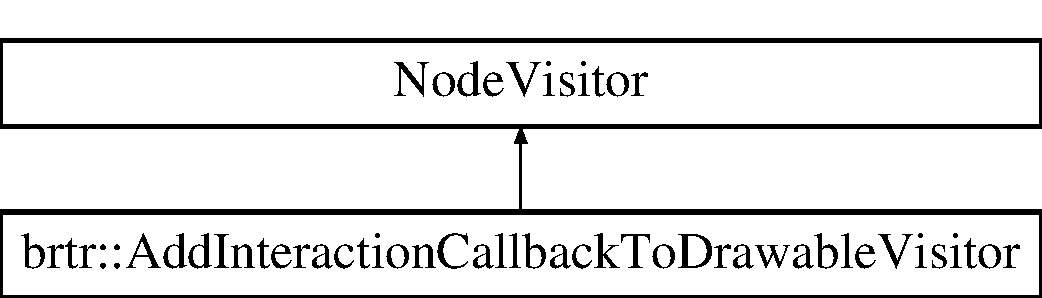
\includegraphics[height=2.000000cm]{classbrtr_1_1_add_interaction_callback_to_drawable_visitor}
\end{center}
\end{figure}
\subsection*{Public Member Functions}
\begin{DoxyCompactItemize}
\item 
\hyperlink{classbrtr_1_1_add_interaction_callback_to_drawable_visitor_a8c1ecd3629ec4f97d4bc2a63c56683d4}{Add\+Interaction\+Callback\+To\+Drawable\+Visitor} (\hyperlink{classbrtr_1_1_base_interaction_callback}{brtr\+::\+Base\+Interaction\+Callback} $\ast$callback\+To\+Add)
\begin{DoxyCompactList}\small\item\em Constructor. \end{DoxyCompactList}\item 
virtual void \hyperlink{classbrtr_1_1_add_interaction_callback_to_drawable_visitor_ace5d2fc7aa7c4a48f59e38728dac628a}{apply} (osg\+::\+Geode \&geode)
\end{DoxyCompactItemize}
\subsection*{Private Attributes}
\begin{DoxyCompactItemize}
\item 
osg\+::ref\+\_\+ptr\\*
$<$ osg\+::\+Default\+User\+Data\+Container $>$ \hyperlink{classbrtr_1_1_add_interaction_callback_to_drawable_visitor_ac23b4a99b1d35c2f7a32f048d4628927}{\+\_\+container\+To\+Add}
\end{DoxyCompactItemize}


\subsection{Detailed Description}
Node\+Visitor for batch replacing all User\+Data\+Container of all Drawables. 

New Container contains the provided Interaction\+Callback. Mainly used for making imported objects (e.\+g. from blender) interact-\/able. \begin{DoxyAuthor}{Author}
Gleb Ostrowski 
\end{DoxyAuthor}
\begin{DoxyVersion}{Version}
1.\+0 
\end{DoxyVersion}
\begin{DoxyDate}{Date}
2014 
\end{DoxyDate}
\begin{DoxyPrecond}{Precondition}
needs a Node which will accept it. Should have some Geode's for this to work 
\end{DoxyPrecond}
\begin{DoxyCopyright}{Copyright}
G\+N\+U Public License. 
\end{DoxyCopyright}


Definition at line \hyperlink{_add_interaction_callback_to_drawable_visitor_8h_source_l00017}{17} of file \hyperlink{_add_interaction_callback_to_drawable_visitor_8h_source}{Add\+Interaction\+Callback\+To\+Drawable\+Visitor.\+h}.



\subsection{Constructor \& Destructor Documentation}
\hypertarget{classbrtr_1_1_add_interaction_callback_to_drawable_visitor_a8c1ecd3629ec4f97d4bc2a63c56683d4}{\index{brtr\+::\+Add\+Interaction\+Callback\+To\+Drawable\+Visitor@{brtr\+::\+Add\+Interaction\+Callback\+To\+Drawable\+Visitor}!Add\+Interaction\+Callback\+To\+Drawable\+Visitor@{Add\+Interaction\+Callback\+To\+Drawable\+Visitor}}
\index{Add\+Interaction\+Callback\+To\+Drawable\+Visitor@{Add\+Interaction\+Callback\+To\+Drawable\+Visitor}!brtr\+::\+Add\+Interaction\+Callback\+To\+Drawable\+Visitor@{brtr\+::\+Add\+Interaction\+Callback\+To\+Drawable\+Visitor}}
\subsubsection[{Add\+Interaction\+Callback\+To\+Drawable\+Visitor}]{\setlength{\rightskip}{0pt plus 5cm}brtr\+::\+Add\+Interaction\+Callback\+To\+Drawable\+Visitor\+::\+Add\+Interaction\+Callback\+To\+Drawable\+Visitor (
\begin{DoxyParamCaption}
\item[{{\bf brtr\+::\+Base\+Interaction\+Callback} $\ast$}]{callback\+To\+Add}
\end{DoxyParamCaption}
)}}\label{classbrtr_1_1_add_interaction_callback_to_drawable_visitor_a8c1ecd3629ec4f97d4bc2a63c56683d4}


Constructor. 


\begin{DoxyParams}{Parameters}
{\em callback\+To\+Add} & the callback which should be add to all drawables in the object \\
\hline
\end{DoxyParams}
\begin{DoxyReturn}{Returns}

\end{DoxyReturn}


Definition at line \hyperlink{_add_interaction_callback_to_drawable_visitor_8cpp_source_l00005}{5} of file \hyperlink{_add_interaction_callback_to_drawable_visitor_8cpp_source}{Add\+Interaction\+Callback\+To\+Drawable\+Visitor.\+cpp}.



\subsection{Member Function Documentation}
\hypertarget{classbrtr_1_1_add_interaction_callback_to_drawable_visitor_ace5d2fc7aa7c4a48f59e38728dac628a}{\index{brtr\+::\+Add\+Interaction\+Callback\+To\+Drawable\+Visitor@{brtr\+::\+Add\+Interaction\+Callback\+To\+Drawable\+Visitor}!apply@{apply}}
\index{apply@{apply}!brtr\+::\+Add\+Interaction\+Callback\+To\+Drawable\+Visitor@{brtr\+::\+Add\+Interaction\+Callback\+To\+Drawable\+Visitor}}
\subsubsection[{apply}]{\setlength{\rightskip}{0pt plus 5cm}void brtr\+::\+Add\+Interaction\+Callback\+To\+Drawable\+Visitor\+::apply (
\begin{DoxyParamCaption}
\item[{osg\+::\+Geode \&}]{geode}
\end{DoxyParamCaption}
)\hspace{0.3cm}{\ttfamily [virtual]}}}\label{classbrtr_1_1_add_interaction_callback_to_drawable_visitor_ace5d2fc7aa7c4a48f59e38728dac628a}


Definition at line \hyperlink{_add_interaction_callback_to_drawable_visitor_8cpp_source_l00011}{11} of file \hyperlink{_add_interaction_callback_to_drawable_visitor_8cpp_source}{Add\+Interaction\+Callback\+To\+Drawable\+Visitor.\+cpp}.



\subsection{Member Data Documentation}
\hypertarget{classbrtr_1_1_add_interaction_callback_to_drawable_visitor_ac23b4a99b1d35c2f7a32f048d4628927}{\index{brtr\+::\+Add\+Interaction\+Callback\+To\+Drawable\+Visitor@{brtr\+::\+Add\+Interaction\+Callback\+To\+Drawable\+Visitor}!\+\_\+container\+To\+Add@{\+\_\+container\+To\+Add}}
\index{\+\_\+container\+To\+Add@{\+\_\+container\+To\+Add}!brtr\+::\+Add\+Interaction\+Callback\+To\+Drawable\+Visitor@{brtr\+::\+Add\+Interaction\+Callback\+To\+Drawable\+Visitor}}
\subsubsection[{\+\_\+container\+To\+Add}]{\setlength{\rightskip}{0pt plus 5cm}osg\+::ref\+\_\+ptr$<$osg\+::\+Default\+User\+Data\+Container$>$ brtr\+::\+Add\+Interaction\+Callback\+To\+Drawable\+Visitor\+::\+\_\+container\+To\+Add\hspace{0.3cm}{\ttfamily [private]}}}\label{classbrtr_1_1_add_interaction_callback_to_drawable_visitor_ac23b4a99b1d35c2f7a32f048d4628927}


Definition at line \hyperlink{_add_interaction_callback_to_drawable_visitor_8h_source_l00028}{28} of file \hyperlink{_add_interaction_callback_to_drawable_visitor_8h_source}{Add\+Interaction\+Callback\+To\+Drawable\+Visitor.\+h}.



The documentation for this class was generated from the following files\+:\begin{DoxyCompactItemize}
\item 
header/\hyperlink{_add_interaction_callback_to_drawable_visitor_8h}{Add\+Interaction\+Callback\+To\+Drawable\+Visitor.\+h}\item 
Util/\hyperlink{_add_interaction_callback_to_drawable_visitor_8cpp}{Add\+Interaction\+Callback\+To\+Drawable\+Visitor.\+cpp}\end{DoxyCompactItemize}

\hypertarget{classbrtr_1_1_add_portal_gun_interaction_callback}{\section{brtr\+:\+:Add\+Portal\+Gun\+Interaction\+Callback Class Reference}
\label{classbrtr_1_1_add_portal_gun_interaction_callback}\index{brtr\+::\+Add\+Portal\+Gun\+Interaction\+Callback@{brtr\+::\+Add\+Portal\+Gun\+Interaction\+Callback}}
}


Interaction\+Callback for adding the portal gun to the players inventar.  




{\ttfamily \#include $<$Add\+Portal\+Gun\+Interaction\+Callback.\+h$>$}

Inheritance diagram for brtr\+:\+:Add\+Portal\+Gun\+Interaction\+Callback\+:\begin{figure}[H]
\begin{center}
\leavevmode
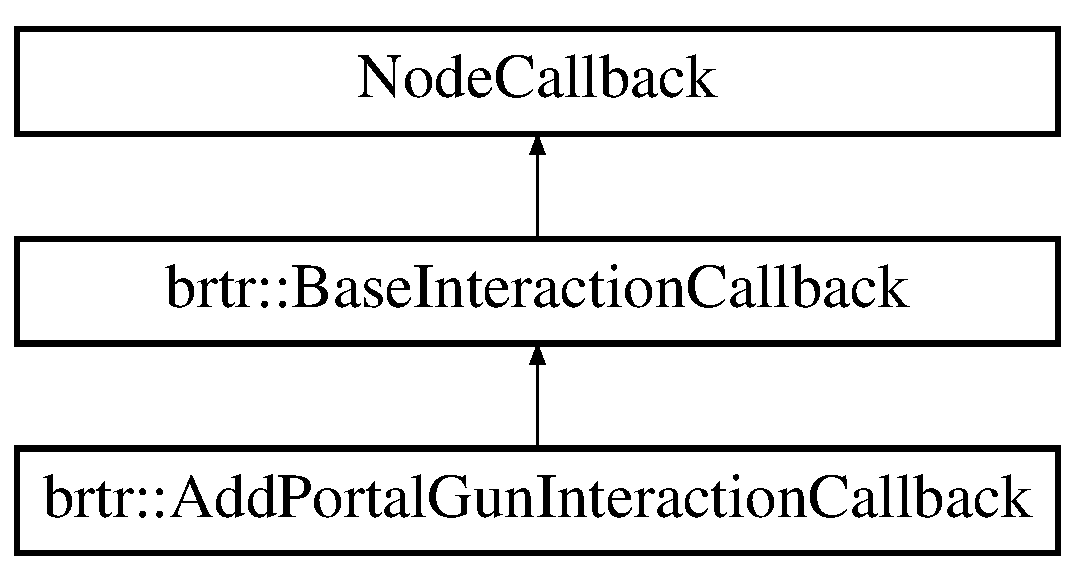
\includegraphics[height=3.000000cm]{classbrtr_1_1_add_portal_gun_interaction_callback}
\end{center}
\end{figure}
\subsection*{Public Member Functions}
\begin{DoxyCompactItemize}
\item 
\hyperlink{classbrtr_1_1_add_portal_gun_interaction_callback_a849f25b53c2a3c81e8201777bf481c96}{Add\+Portal\+Gun\+Interaction\+Callback} (osg\+::\+Node $\ast$weapon\+H\+U\+D, osg\+::\+Camera $\ast$hud\+Cam, osg\+::\+Switch $\ast$switcher, int width, int height)
\begin{DoxyCompactList}\small\item\em Constructor. \end{DoxyCompactList}\item 
virtual void \hyperlink{classbrtr_1_1_add_portal_gun_interaction_callback_aa0db50622c7ae1cd25f8554c916137db}{set\+Text} ()
\begin{DoxyCompactList}\small\item\em sets the text on screen. Subclasses must override to set its own (info)text \end{DoxyCompactList}\end{DoxyCompactItemize}
\subsection*{Protected Member Functions}
\begin{DoxyCompactItemize}
\item 
virtual void \hyperlink{classbrtr_1_1_add_portal_gun_interaction_callback_a9b6571b0295f7e12425b57ff0262dbd4}{interact} (osg\+::\+Node $\ast$, osg\+::\+Node\+Visitor $\ast$)
\begin{DoxyCompactList}\small\item\em the interaction logic must be implemented be the children in this method \end{DoxyCompactList}\end{DoxyCompactItemize}
\subsection*{Private Attributes}
\begin{DoxyCompactItemize}
\item 
osg\+::ref\+\_\+ptr$<$ osg\+::\+Switch $>$ \hyperlink{classbrtr_1_1_add_portal_gun_interaction_callback_ac110a98cbe720e599b344d9940702597}{\+\_\+switcher}
\end{DoxyCompactItemize}
\subsection*{Additional Inherited Members}


\subsection{Detailed Description}
Interaction\+Callback for adding the portal gun to the players inventar. 

\begin{DoxyAuthor}{Author}
Gleb Ostrowski 
\end{DoxyAuthor}
\begin{DoxyVersion}{Version}
1.\+0 
\end{DoxyVersion}
\begin{DoxyDate}{Date}
2014 
\end{DoxyDate}
\begin{DoxyCopyright}{Copyright}
G\+N\+U Public License. 
\end{DoxyCopyright}


Definition at line \hyperlink{_add_portal_gun_interaction_callback_8h_source_l00014}{14} of file \hyperlink{_add_portal_gun_interaction_callback_8h_source}{Add\+Portal\+Gun\+Interaction\+Callback.\+h}.



\subsection{Constructor \& Destructor Documentation}
\hypertarget{classbrtr_1_1_add_portal_gun_interaction_callback_a849f25b53c2a3c81e8201777bf481c96}{\index{brtr\+::\+Add\+Portal\+Gun\+Interaction\+Callback@{brtr\+::\+Add\+Portal\+Gun\+Interaction\+Callback}!Add\+Portal\+Gun\+Interaction\+Callback@{Add\+Portal\+Gun\+Interaction\+Callback}}
\index{Add\+Portal\+Gun\+Interaction\+Callback@{Add\+Portal\+Gun\+Interaction\+Callback}!brtr\+::\+Add\+Portal\+Gun\+Interaction\+Callback@{brtr\+::\+Add\+Portal\+Gun\+Interaction\+Callback}}
\subsubsection[{Add\+Portal\+Gun\+Interaction\+Callback}]{\setlength{\rightskip}{0pt plus 5cm}brtr\+::\+Add\+Portal\+Gun\+Interaction\+Callback\+::\+Add\+Portal\+Gun\+Interaction\+Callback (
\begin{DoxyParamCaption}
\item[{osg\+::\+Node $\ast$}]{weapon\+H\+U\+D, }
\item[{osg\+::\+Camera $\ast$}]{hud\+Cam, }
\item[{osg\+::\+Switch $\ast$}]{switcher, }
\item[{int}]{width, }
\item[{int}]{height}
\end{DoxyParamCaption}
)}}\label{classbrtr_1_1_add_portal_gun_interaction_callback_a849f25b53c2a3c81e8201777bf481c96}


Constructor. 


\begin{DoxyParams}{Parameters}
{\em weapon\+H\+U\+D} & weapon\+H\+U\+D which provides the method to add the portalgun to it \\
\hline
{\em hud\+Cam} & \\
\hline
{\em switcher} & switch-\/node which contains the portal\+Gun object, will be switched to off upon interaction, removing the portal Gun from the world \\
\hline
{\em width} & screen\+Width \\
\hline
{\em height} & screen\+Height \\
\hline
\end{DoxyParams}
\begin{DoxyReturn}{Returns}

\end{DoxyReturn}


Definition at line \hyperlink{_add_portal_gun_interaction_callback_8cpp_source_l00005}{5} of file \hyperlink{_add_portal_gun_interaction_callback_8cpp_source}{Add\+Portal\+Gun\+Interaction\+Callback.\+cpp}.



\subsection{Member Function Documentation}
\hypertarget{classbrtr_1_1_add_portal_gun_interaction_callback_a9b6571b0295f7e12425b57ff0262dbd4}{\index{brtr\+::\+Add\+Portal\+Gun\+Interaction\+Callback@{brtr\+::\+Add\+Portal\+Gun\+Interaction\+Callback}!interact@{interact}}
\index{interact@{interact}!brtr\+::\+Add\+Portal\+Gun\+Interaction\+Callback@{brtr\+::\+Add\+Portal\+Gun\+Interaction\+Callback}}
\subsubsection[{interact}]{\setlength{\rightskip}{0pt plus 5cm}void brtr\+::\+Add\+Portal\+Gun\+Interaction\+Callback\+::interact (
\begin{DoxyParamCaption}
\item[{osg\+::\+Node $\ast$}]{, }
\item[{osg\+::\+Node\+Visitor $\ast$}]{}
\end{DoxyParamCaption}
)\hspace{0.3cm}{\ttfamily [protected]}, {\ttfamily [virtual]}}}\label{classbrtr_1_1_add_portal_gun_interaction_callback_a9b6571b0295f7e12425b57ff0262dbd4}


the interaction logic must be implemented be the children in this method 



Implements \hyperlink{classbrtr_1_1_base_interaction_callback_a3ed50c9c1725f932e0b78c90ba24e1ed}{brtr\+::\+Base\+Interaction\+Callback}.



Definition at line \hyperlink{_add_portal_gun_interaction_callback_8cpp_source_l00013}{13} of file \hyperlink{_add_portal_gun_interaction_callback_8cpp_source}{Add\+Portal\+Gun\+Interaction\+Callback.\+cpp}.

\hypertarget{classbrtr_1_1_add_portal_gun_interaction_callback_aa0db50622c7ae1cd25f8554c916137db}{\index{brtr\+::\+Add\+Portal\+Gun\+Interaction\+Callback@{brtr\+::\+Add\+Portal\+Gun\+Interaction\+Callback}!set\+Text@{set\+Text}}
\index{set\+Text@{set\+Text}!brtr\+::\+Add\+Portal\+Gun\+Interaction\+Callback@{brtr\+::\+Add\+Portal\+Gun\+Interaction\+Callback}}
\subsubsection[{set\+Text}]{\setlength{\rightskip}{0pt plus 5cm}void brtr\+::\+Add\+Portal\+Gun\+Interaction\+Callback\+::set\+Text (
\begin{DoxyParamCaption}
{}
\end{DoxyParamCaption}
)\hspace{0.3cm}{\ttfamily [virtual]}}}\label{classbrtr_1_1_add_portal_gun_interaction_callback_aa0db50622c7ae1cd25f8554c916137db}


sets the text on screen. Subclasses must override to set its own (info)text 



Implements \hyperlink{classbrtr_1_1_base_interaction_callback_a0fe57e329f044e21d49041c861435ad8}{brtr\+::\+Base\+Interaction\+Callback}.



Definition at line \hyperlink{_add_portal_gun_interaction_callback_8cpp_source_l00009}{9} of file \hyperlink{_add_portal_gun_interaction_callback_8cpp_source}{Add\+Portal\+Gun\+Interaction\+Callback.\+cpp}.



\subsection{Member Data Documentation}
\hypertarget{classbrtr_1_1_add_portal_gun_interaction_callback_ac110a98cbe720e599b344d9940702597}{\index{brtr\+::\+Add\+Portal\+Gun\+Interaction\+Callback@{brtr\+::\+Add\+Portal\+Gun\+Interaction\+Callback}!\+\_\+switcher@{\+\_\+switcher}}
\index{\+\_\+switcher@{\+\_\+switcher}!brtr\+::\+Add\+Portal\+Gun\+Interaction\+Callback@{brtr\+::\+Add\+Portal\+Gun\+Interaction\+Callback}}
\subsubsection[{\+\_\+switcher}]{\setlength{\rightskip}{0pt plus 5cm}osg\+::ref\+\_\+ptr$<$osg\+::\+Switch$>$ brtr\+::\+Add\+Portal\+Gun\+Interaction\+Callback\+::\+\_\+switcher\hspace{0.3cm}{\ttfamily [private]}}}\label{classbrtr_1_1_add_portal_gun_interaction_callback_ac110a98cbe720e599b344d9940702597}


Definition at line \hyperlink{_add_portal_gun_interaction_callback_8h_source_l00032}{32} of file \hyperlink{_add_portal_gun_interaction_callback_8h_source}{Add\+Portal\+Gun\+Interaction\+Callback.\+h}.



The documentation for this class was generated from the following files\+:\begin{DoxyCompactItemize}
\item 
header/\hyperlink{_add_portal_gun_interaction_callback_8h}{Add\+Portal\+Gun\+Interaction\+Callback.\+h}\item 
Callbacks/\hyperlink{_add_portal_gun_interaction_callback_8cpp}{Add\+Portal\+Gun\+Interaction\+Callback.\+cpp}\end{DoxyCompactItemize}

\hypertarget{class_animation_creator}{\section{Animation\+Creator Class Reference}
\label{class_animation_creator}\index{Animation\+Creator@{Animation\+Creator}}
}


{\ttfamily \#include $<$Animation\+Creater.\+h$>$}

\subsection*{Public Member Functions}
\begin{DoxyCompactItemize}
\item 
double \hyperlink{class_animation_creator_a03e8400c38e8710ee20fd44f57ab1903}{get\+Angle\+Rad} (osg\+::\+Vec3 point\+A, osg\+::\+Vec3 point\+B)
\begin{DoxyCompactList}\small\item\em Creator of the Animation Path for the Train-\/\+Simulation. \end{DoxyCompactList}\item 
osg\+::\+Animation\+Path $\ast$ \hyperlink{class_animation_creator_aca52f3472d0be7043c63ff5ede8084aa}{create\+Animation\+Path} (float time)
\begin{DoxyCompactList}\small\item\em Creates the animation path. \end{DoxyCompactList}\end{DoxyCompactItemize}


\subsection{Detailed Description}


Definition at line \hyperlink{_animation_creater_8h_source_l00005}{5} of file \hyperlink{_animation_creater_8h_source}{Animation\+Creater.\+h}.



\subsection{Member Function Documentation}
\hypertarget{class_animation_creator_aca52f3472d0be7043c63ff5ede8084aa}{\index{Animation\+Creator@{Animation\+Creator}!create\+Animation\+Path@{create\+Animation\+Path}}
\index{create\+Animation\+Path@{create\+Animation\+Path}!Animation\+Creator@{Animation\+Creator}}
\subsubsection[{create\+Animation\+Path}]{\setlength{\rightskip}{0pt plus 5cm}osg\+::\+Animation\+Path $\ast$ Animation\+Creator\+::create\+Animation\+Path (
\begin{DoxyParamCaption}
\item[{float}]{time}
\end{DoxyParamCaption}
)}}\label{class_animation_creator_aca52f3472d0be7043c63ff5ede8084aa}


Creates the animation path. 

The Method creates the Train Animation\+Path. Each vector will be included in the Animation\+Path, together with the correct rotation between two points.


\begin{DoxyParams}{Parameters}
{\em time} & is the time that the train will take between two vectors, low time = fast train. \\
\hline
\end{DoxyParams}
\begin{DoxyReturn}{Returns}
the complete Animation\+Path for the train 
\end{DoxyReturn}


Definition at line \hyperlink{_animation_creater_8cpp_source_l00040}{40} of file \hyperlink{_animation_creater_8cpp_source}{Animation\+Creater.\+cpp}.

\hypertarget{class_animation_creator_a03e8400c38e8710ee20fd44f57ab1903}{\index{Animation\+Creator@{Animation\+Creator}!get\+Angle\+Rad@{get\+Angle\+Rad}}
\index{get\+Angle\+Rad@{get\+Angle\+Rad}!Animation\+Creator@{Animation\+Creator}}
\subsubsection[{get\+Angle\+Rad}]{\setlength{\rightskip}{0pt plus 5cm}double Animation\+Creator\+::get\+Angle\+Rad (
\begin{DoxyParamCaption}
\item[{osg\+::\+Vec3}]{point\+A, }
\item[{osg\+::\+Vec3}]{point\+B}
\end{DoxyParamCaption}
)}}\label{class_animation_creator_a03e8400c38e8710ee20fd44f57ab1903}


Creator of the Animation Path for the Train-\/\+Simulation. 

\begin{DoxyAuthor}{Author}
Philip Sauer 
\end{DoxyAuthor}
\begin{DoxyVersion}{Version}
1.\+0 
\end{DoxyVersion}
\begin{DoxyDate}{Date}
2014 Calculate the angle between two Vectors
\end{DoxyDate}
The Method calculates the dotproduct between two vectors and devides it with the length of both vectors. ( vector\+A $\ast$ vector\+B ) / ( $\vert$vector\+A$\vert$ $\ast$ $\vert$vector\+B$\vert$ )


\begin{DoxyParams}{Parameters}
{\em point\+A} & the starting Vector \\
\hline
{\em point\+B} & the end Vector \\
\hline
\end{DoxyParams}
\begin{DoxyReturn}{Returns}
the angle in radian 
\end{DoxyReturn}


Definition at line \hyperlink{_animation_creater_8cpp_source_l00016}{16} of file \hyperlink{_animation_creater_8cpp_source}{Animation\+Creater.\+cpp}.



The documentation for this class was generated from the following files\+:\begin{DoxyCompactItemize}
\item 
header/\hyperlink{_animation_creater_8h}{Animation\+Creater.\+h}\item 
Animation/\hyperlink{_animation_creater_8cpp}{Animation\+Creater.\+cpp}\end{DoxyCompactItemize}

\hypertarget{classbrtr_1_1_base_interaction_callback}{\section{brtr\+:\+:Base\+Interaction\+Callback Class Reference}
\label{classbrtr_1_1_base_interaction_callback}\index{brtr\+::\+Base\+Interaction\+Callback@{brtr\+::\+Base\+Interaction\+Callback}}
}


This is the Template\+Class for Interaction\+Callbacks.  




{\ttfamily \#include $<$Base\+Interaction\+Callback.\+h$>$}

Inheritance diagram for brtr\+:\+:Base\+Interaction\+Callback\+:\begin{figure}[H]
\begin{center}
\leavevmode
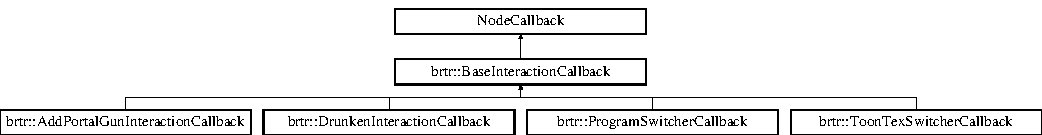
\includegraphics[height=1.802575cm]{classbrtr_1_1_base_interaction_callback}
\end{center}
\end{figure}
\subsection*{Public Member Functions}
\begin{DoxyCompactItemize}
\item 
\hyperlink{classbrtr_1_1_base_interaction_callback_afc863306967933e0ebef5f7322fab06e}{Base\+Interaction\+Callback} (osg\+::\+Node $\ast$attach\+To, osg\+::\+Camera $\ast$hud\+Cam, int width, int height)
\begin{DoxyCompactList}\small\item\em Constructor. \end{DoxyCompactList}\item 
virtual void \hyperlink{classbrtr_1_1_base_interaction_callback_ab2cf0f22fcc9e79ecda29a547edb5084}{operator()} (osg\+::\+Node $\ast$node, osg\+::\+Node\+Visitor $\ast$nv)
\item 
virtual void \hyperlink{classbrtr_1_1_base_interaction_callback_a0fe57e329f044e21d49041c861435ad8}{set\+Text} ()=0
\begin{DoxyCompactList}\small\item\em sets the text on screen. Subclasses must override to set its own (info)text \end{DoxyCompactList}\item 
void \hyperlink{classbrtr_1_1_base_interaction_callback_ad74fe9ac5d86c7f23d18614d5abb1003}{clear\+Text} ()
\item 
void \hyperlink{classbrtr_1_1_base_interaction_callback_a95ede7c8aa0dc1e067ae64615ecb23db}{reactivate} ()
\item 
osg\+::ref\+\_\+ptr$<$ osg\+::\+Node $>$ \hyperlink{classbrtr_1_1_base_interaction_callback_aafca24ccde1cf21f4132f65a83e0b2bc}{get\+Node} () const 
\item 
void \hyperlink{classbrtr_1_1_base_interaction_callback_a420a1977c954850dbe66a189908cde80}{set\+Node} (osg\+::ref\+\_\+ptr$<$ osg\+::\+Node $>$ val)
\end{DoxyCompactItemize}
\subsection*{Protected Member Functions}
\begin{DoxyCompactItemize}
\item 
virtual void \hyperlink{classbrtr_1_1_base_interaction_callback_a3ed50c9c1725f932e0b78c90ba24e1ed}{interact} (osg\+::\+Node $\ast$, osg\+::\+Node\+Visitor $\ast$)=0
\begin{DoxyCompactList}\small\item\em the interaction logic must be implemented be the children in this method \end{DoxyCompactList}\end{DoxyCompactItemize}
\subsection*{Protected Attributes}
\begin{DoxyCompactItemize}
\item 
osg\+::ref\+\_\+ptr$<$ osg\+::\+Node $>$ \hyperlink{classbrtr_1_1_base_interaction_callback_a6666bae9f8f89ebbf75637c922ebfb54}{\+\_\+attach\+To}
\item 
osg\+::ref\+\_\+ptr$<$ osg\+::\+Camera $>$ \hyperlink{classbrtr_1_1_base_interaction_callback_a0bca3b64724235e08740be94fe4acc8d}{\+\_\+hud\+Cam}
\item 
bool \hyperlink{classbrtr_1_1_base_interaction_callback_a2f36052886ec60a227e0734bfbc4bdbb}{\+\_\+done}
\item 
osg\+::ref\+\_\+ptr$<$ osg\+Text\+::\+Text $>$ \hyperlink{classbrtr_1_1_base_interaction_callback_af60dece4300b09fafe3c048397122cbd}{\+\_\+text}
\end{DoxyCompactItemize}


\subsection{Detailed Description}
This is the Template\+Class for Interaction\+Callbacks. 

Interaction\+Callbacks are set as an User\+Object in an User\+Data\+Container of a Geometry.~\newline
 Furthermore, the right Node\+Mask (\hyperlink{namespacebrtr_a2060f4d70c0e3bc7e2e35f82e279a40d}{brtr\+::interaction\+Mask}) must be set. ~\newline
 Every subclass must override the \hyperlink{classbrtr_1_1_base_interaction_callback_a0fe57e329f044e21d49041c861435ad8}{set\+Text()} and \hyperlink{classbrtr_1_1_base_interaction_callback_a3ed50c9c1725f932e0b78c90ba24e1ed}{interact()} method. ~\newline
 After the child is finished with its work, it must set the done-\/flag to the value true ~\newline
 The client must check if there is a valid Geometry with a valid Interaction\+Callback and call ~\newline
 the set\+Text Method to set the text on screen. If the user interacts (e.\+g by clicking a mouse button) ~\newline
 the client must attach the callback to the node with \hyperlink{classbrtr_1_1_base_interaction_callback_aafca24ccde1cf21f4132f65a83e0b2bc}{get\+Node()}-\/$>$add\+Update\+Callback(), if its not already attached. ~\newline
 In this case the client must call \hyperlink{classbrtr_1_1_base_interaction_callback_a95ede7c8aa0dc1e067ae64615ecb23db}{reactivate()} to reactivate the callback. (which basicly sets the done flag back to false) ~\newline
 \hyperlink{classbrtr_1_1_base_interaction_callback_ad74fe9ac5d86c7f23d18614d5abb1003}{clear\+Text()} should be called, if the clients wants to remove the message from the screen (e.\+g. if the player no longer looks at the geometry).

\begin{DoxyAuthor}{Author}
Gleb Ostrowski 
\end{DoxyAuthor}
\begin{DoxyVersion}{Version}
1.\+0 
\end{DoxyVersion}
\begin{DoxyDate}{Date}
2014 
\end{DoxyDate}
\begin{DoxyCopyright}{Copyright}
G\+N\+U Public License. 
\end{DoxyCopyright}


Definition at line \hyperlink{_base_interaction_callback_8h_source_l00024}{24} of file \hyperlink{_base_interaction_callback_8h_source}{Base\+Interaction\+Callback.\+h}.



\subsection{Constructor \& Destructor Documentation}
\hypertarget{classbrtr_1_1_base_interaction_callback_afc863306967933e0ebef5f7322fab06e}{\index{brtr\+::\+Base\+Interaction\+Callback@{brtr\+::\+Base\+Interaction\+Callback}!Base\+Interaction\+Callback@{Base\+Interaction\+Callback}}
\index{Base\+Interaction\+Callback@{Base\+Interaction\+Callback}!brtr\+::\+Base\+Interaction\+Callback@{brtr\+::\+Base\+Interaction\+Callback}}
\subsubsection[{Base\+Interaction\+Callback}]{\setlength{\rightskip}{0pt plus 5cm}brtr\+::\+Base\+Interaction\+Callback\+::\+Base\+Interaction\+Callback (
\begin{DoxyParamCaption}
\item[{osg\+::\+Node $\ast$}]{attach\+To, }
\item[{osg\+::\+Camera $\ast$}]{hud\+Cam, }
\item[{int}]{width, }
\item[{int}]{height}
\end{DoxyParamCaption}
)}}\label{classbrtr_1_1_base_interaction_callback_afc863306967933e0ebef5f7322fab06e}


Constructor. 


\begin{DoxyParams}{Parameters}
{\em attach\+To} & the node the Callback will be attached to upon interaction \\
\hline
{\em hud\+Cam} & the H\+U\+D\+Cam, where the text will appear \\
\hline
{\em width} & screen\+Width \\
\hline
{\em height} & screen\+Height \\
\hline
\end{DoxyParams}


Definition at line \hyperlink{_base_interaction_callback_8cpp_source_l00006}{6} of file \hyperlink{_base_interaction_callback_8cpp_source}{Base\+Interaction\+Callback.\+cpp}.



\subsection{Member Function Documentation}
\hypertarget{classbrtr_1_1_base_interaction_callback_ad74fe9ac5d86c7f23d18614d5abb1003}{\index{brtr\+::\+Base\+Interaction\+Callback@{brtr\+::\+Base\+Interaction\+Callback}!clear\+Text@{clear\+Text}}
\index{clear\+Text@{clear\+Text}!brtr\+::\+Base\+Interaction\+Callback@{brtr\+::\+Base\+Interaction\+Callback}}
\subsubsection[{clear\+Text}]{\setlength{\rightskip}{0pt plus 5cm}void brtr\+::\+Base\+Interaction\+Callback\+::clear\+Text (
\begin{DoxyParamCaption}
{}
\end{DoxyParamCaption}
)}}\label{classbrtr_1_1_base_interaction_callback_ad74fe9ac5d86c7f23d18614d5abb1003}


Definition at line \hyperlink{_base_interaction_callback_8cpp_source_l00031}{31} of file \hyperlink{_base_interaction_callback_8cpp_source}{Base\+Interaction\+Callback.\+cpp}.

\hypertarget{classbrtr_1_1_base_interaction_callback_aafca24ccde1cf21f4132f65a83e0b2bc}{\index{brtr\+::\+Base\+Interaction\+Callback@{brtr\+::\+Base\+Interaction\+Callback}!get\+Node@{get\+Node}}
\index{get\+Node@{get\+Node}!brtr\+::\+Base\+Interaction\+Callback@{brtr\+::\+Base\+Interaction\+Callback}}
\subsubsection[{get\+Node}]{\setlength{\rightskip}{0pt plus 5cm}osg\+::ref\+\_\+ptr$<$ osg\+::\+Node $>$ brtr\+::\+Base\+Interaction\+Callback\+::get\+Node (
\begin{DoxyParamCaption}
{}
\end{DoxyParamCaption}
) const}}\label{classbrtr_1_1_base_interaction_callback_aafca24ccde1cf21f4132f65a83e0b2bc}


Definition at line \hyperlink{_base_interaction_callback_8cpp_source_l00027}{27} of file \hyperlink{_base_interaction_callback_8cpp_source}{Base\+Interaction\+Callback.\+cpp}.

\hypertarget{classbrtr_1_1_base_interaction_callback_a3ed50c9c1725f932e0b78c90ba24e1ed}{\index{brtr\+::\+Base\+Interaction\+Callback@{brtr\+::\+Base\+Interaction\+Callback}!interact@{interact}}
\index{interact@{interact}!brtr\+::\+Base\+Interaction\+Callback@{brtr\+::\+Base\+Interaction\+Callback}}
\subsubsection[{interact}]{\setlength{\rightskip}{0pt plus 5cm}virtual void brtr\+::\+Base\+Interaction\+Callback\+::interact (
\begin{DoxyParamCaption}
\item[{osg\+::\+Node $\ast$}]{, }
\item[{osg\+::\+Node\+Visitor $\ast$}]{}
\end{DoxyParamCaption}
)\hspace{0.3cm}{\ttfamily [protected]}, {\ttfamily [pure virtual]}}}\label{classbrtr_1_1_base_interaction_callback_a3ed50c9c1725f932e0b78c90ba24e1ed}


the interaction logic must be implemented be the children in this method 



Implemented in \hyperlink{classbrtr_1_1_program_switcher_callback_a06dd3fc2b09d3138e67599d8d56db62a}{brtr\+::\+Program\+Switcher\+Callback}, \hyperlink{classbrtr_1_1_toon_tex_switcher_callback_a97047bc2817ddfecc2c1531d22e289fd}{brtr\+::\+Toon\+Tex\+Switcher\+Callback}, \hyperlink{classbrtr_1_1_drunken_interaction_callback_a86e4062f00a33768f752c1c5fa50c291}{brtr\+::\+Drunken\+Interaction\+Callback}, and \hyperlink{classbrtr_1_1_add_portal_gun_interaction_callback_a9b6571b0295f7e12425b57ff0262dbd4}{brtr\+::\+Add\+Portal\+Gun\+Interaction\+Callback}.

\hypertarget{classbrtr_1_1_base_interaction_callback_ab2cf0f22fcc9e79ecda29a547edb5084}{\index{brtr\+::\+Base\+Interaction\+Callback@{brtr\+::\+Base\+Interaction\+Callback}!operator()@{operator()}}
\index{operator()@{operator()}!brtr\+::\+Base\+Interaction\+Callback@{brtr\+::\+Base\+Interaction\+Callback}}
\subsubsection[{operator()}]{\setlength{\rightskip}{0pt plus 5cm}void brtr\+::\+Base\+Interaction\+Callback\+::operator() (
\begin{DoxyParamCaption}
\item[{osg\+::\+Node $\ast$}]{node, }
\item[{osg\+::\+Node\+Visitor $\ast$}]{nv}
\end{DoxyParamCaption}
)\hspace{0.3cm}{\ttfamily [virtual]}}}\label{classbrtr_1_1_base_interaction_callback_ab2cf0f22fcc9e79ecda29a547edb5084}


Definition at line \hyperlink{_base_interaction_callback_8cpp_source_l00016}{16} of file \hyperlink{_base_interaction_callback_8cpp_source}{Base\+Interaction\+Callback.\+cpp}.

\hypertarget{classbrtr_1_1_base_interaction_callback_a95ede7c8aa0dc1e067ae64615ecb23db}{\index{brtr\+::\+Base\+Interaction\+Callback@{brtr\+::\+Base\+Interaction\+Callback}!reactivate@{reactivate}}
\index{reactivate@{reactivate}!brtr\+::\+Base\+Interaction\+Callback@{brtr\+::\+Base\+Interaction\+Callback}}
\subsubsection[{reactivate}]{\setlength{\rightskip}{0pt plus 5cm}void brtr\+::\+Base\+Interaction\+Callback\+::reactivate (
\begin{DoxyParamCaption}
{}
\end{DoxyParamCaption}
)}}\label{classbrtr_1_1_base_interaction_callback_a95ede7c8aa0dc1e067ae64615ecb23db}


Definition at line \hyperlink{_base_interaction_callback_8cpp_source_l00035}{35} of file \hyperlink{_base_interaction_callback_8cpp_source}{Base\+Interaction\+Callback.\+cpp}.

\hypertarget{classbrtr_1_1_base_interaction_callback_a420a1977c954850dbe66a189908cde80}{\index{brtr\+::\+Base\+Interaction\+Callback@{brtr\+::\+Base\+Interaction\+Callback}!set\+Node@{set\+Node}}
\index{set\+Node@{set\+Node}!brtr\+::\+Base\+Interaction\+Callback@{brtr\+::\+Base\+Interaction\+Callback}}
\subsubsection[{set\+Node}]{\setlength{\rightskip}{0pt plus 5cm}void brtr\+::\+Base\+Interaction\+Callback\+::set\+Node (
\begin{DoxyParamCaption}
\item[{osg\+::ref\+\_\+ptr$<$ osg\+::\+Node $>$}]{val}
\end{DoxyParamCaption}
)}}\label{classbrtr_1_1_base_interaction_callback_a420a1977c954850dbe66a189908cde80}


Definition at line \hyperlink{_base_interaction_callback_8cpp_source_l00023}{23} of file \hyperlink{_base_interaction_callback_8cpp_source}{Base\+Interaction\+Callback.\+cpp}.

\hypertarget{classbrtr_1_1_base_interaction_callback_a0fe57e329f044e21d49041c861435ad8}{\index{brtr\+::\+Base\+Interaction\+Callback@{brtr\+::\+Base\+Interaction\+Callback}!set\+Text@{set\+Text}}
\index{set\+Text@{set\+Text}!brtr\+::\+Base\+Interaction\+Callback@{brtr\+::\+Base\+Interaction\+Callback}}
\subsubsection[{set\+Text}]{\setlength{\rightskip}{0pt plus 5cm}virtual void brtr\+::\+Base\+Interaction\+Callback\+::set\+Text (
\begin{DoxyParamCaption}
{}
\end{DoxyParamCaption}
)\hspace{0.3cm}{\ttfamily [pure virtual]}}}\label{classbrtr_1_1_base_interaction_callback_a0fe57e329f044e21d49041c861435ad8}


sets the text on screen. Subclasses must override to set its own (info)text 



Implemented in \hyperlink{classbrtr_1_1_program_switcher_callback_a2202619d98a432578c8ed7342b957638}{brtr\+::\+Program\+Switcher\+Callback}, \hyperlink{classbrtr_1_1_toon_tex_switcher_callback_aad13301231829b5c28f14910d4d44355}{brtr\+::\+Toon\+Tex\+Switcher\+Callback}, \hyperlink{classbrtr_1_1_drunken_interaction_callback_a71b86fc410bf2965ca998eff1350cfaf}{brtr\+::\+Drunken\+Interaction\+Callback}, and \hyperlink{classbrtr_1_1_add_portal_gun_interaction_callback_aa0db50622c7ae1cd25f8554c916137db}{brtr\+::\+Add\+Portal\+Gun\+Interaction\+Callback}.



\subsection{Member Data Documentation}
\hypertarget{classbrtr_1_1_base_interaction_callback_a6666bae9f8f89ebbf75637c922ebfb54}{\index{brtr\+::\+Base\+Interaction\+Callback@{brtr\+::\+Base\+Interaction\+Callback}!\+\_\+attach\+To@{\+\_\+attach\+To}}
\index{\+\_\+attach\+To@{\+\_\+attach\+To}!brtr\+::\+Base\+Interaction\+Callback@{brtr\+::\+Base\+Interaction\+Callback}}
\subsubsection[{\+\_\+attach\+To}]{\setlength{\rightskip}{0pt plus 5cm}osg\+::ref\+\_\+ptr$<$osg\+::\+Node$>$ brtr\+::\+Base\+Interaction\+Callback\+::\+\_\+attach\+To\hspace{0.3cm}{\ttfamily [protected]}}}\label{classbrtr_1_1_base_interaction_callback_a6666bae9f8f89ebbf75637c922ebfb54}


Definition at line \hyperlink{_base_interaction_callback_8h_source_l00051}{51} of file \hyperlink{_base_interaction_callback_8h_source}{Base\+Interaction\+Callback.\+h}.

\hypertarget{classbrtr_1_1_base_interaction_callback_a2f36052886ec60a227e0734bfbc4bdbb}{\index{brtr\+::\+Base\+Interaction\+Callback@{brtr\+::\+Base\+Interaction\+Callback}!\+\_\+done@{\+\_\+done}}
\index{\+\_\+done@{\+\_\+done}!brtr\+::\+Base\+Interaction\+Callback@{brtr\+::\+Base\+Interaction\+Callback}}
\subsubsection[{\+\_\+done}]{\setlength{\rightskip}{0pt plus 5cm}bool brtr\+::\+Base\+Interaction\+Callback\+::\+\_\+done\hspace{0.3cm}{\ttfamily [protected]}}}\label{classbrtr_1_1_base_interaction_callback_a2f36052886ec60a227e0734bfbc4bdbb}


Definition at line \hyperlink{_base_interaction_callback_8h_source_l00053}{53} of file \hyperlink{_base_interaction_callback_8h_source}{Base\+Interaction\+Callback.\+h}.

\hypertarget{classbrtr_1_1_base_interaction_callback_a0bca3b64724235e08740be94fe4acc8d}{\index{brtr\+::\+Base\+Interaction\+Callback@{brtr\+::\+Base\+Interaction\+Callback}!\+\_\+hud\+Cam@{\+\_\+hud\+Cam}}
\index{\+\_\+hud\+Cam@{\+\_\+hud\+Cam}!brtr\+::\+Base\+Interaction\+Callback@{brtr\+::\+Base\+Interaction\+Callback}}
\subsubsection[{\+\_\+hud\+Cam}]{\setlength{\rightskip}{0pt plus 5cm}osg\+::ref\+\_\+ptr$<$osg\+::\+Camera$>$ brtr\+::\+Base\+Interaction\+Callback\+::\+\_\+hud\+Cam\hspace{0.3cm}{\ttfamily [protected]}}}\label{classbrtr_1_1_base_interaction_callback_a0bca3b64724235e08740be94fe4acc8d}


Definition at line \hyperlink{_base_interaction_callback_8h_source_l00052}{52} of file \hyperlink{_base_interaction_callback_8h_source}{Base\+Interaction\+Callback.\+h}.

\hypertarget{classbrtr_1_1_base_interaction_callback_af60dece4300b09fafe3c048397122cbd}{\index{brtr\+::\+Base\+Interaction\+Callback@{brtr\+::\+Base\+Interaction\+Callback}!\+\_\+text@{\+\_\+text}}
\index{\+\_\+text@{\+\_\+text}!brtr\+::\+Base\+Interaction\+Callback@{brtr\+::\+Base\+Interaction\+Callback}}
\subsubsection[{\+\_\+text}]{\setlength{\rightskip}{0pt plus 5cm}osg\+::ref\+\_\+ptr$<$osg\+Text\+::\+Text$>$ brtr\+::\+Base\+Interaction\+Callback\+::\+\_\+text\hspace{0.3cm}{\ttfamily [protected]}}}\label{classbrtr_1_1_base_interaction_callback_af60dece4300b09fafe3c048397122cbd}


Definition at line \hyperlink{_base_interaction_callback_8h_source_l00054}{54} of file \hyperlink{_base_interaction_callback_8h_source}{Base\+Interaction\+Callback.\+h}.



The documentation for this class was generated from the following files\+:\begin{DoxyCompactItemize}
\item 
header/\hyperlink{_base_interaction_callback_8h}{Base\+Interaction\+Callback.\+h}\item 
Callbacks/\hyperlink{_base_interaction_callback_8cpp}{Base\+Interaction\+Callback.\+cpp}\end{DoxyCompactItemize}

\hypertarget{classbrtr_1_1_bench}{\section{brtr\+:\+:Bench Class Reference}
\label{classbrtr_1_1_bench}\index{brtr\+::\+Bench@{brtr\+::\+Bench}}
}


\hyperlink{classbrtr_1_1_bench}{Bench} class, creates a bench Object.  




{\ttfamily \#include $<$Bench.\+h$>$}

Inheritance diagram for brtr\+:\+:Bench\+:\begin{figure}[H]
\begin{center}
\leavevmode
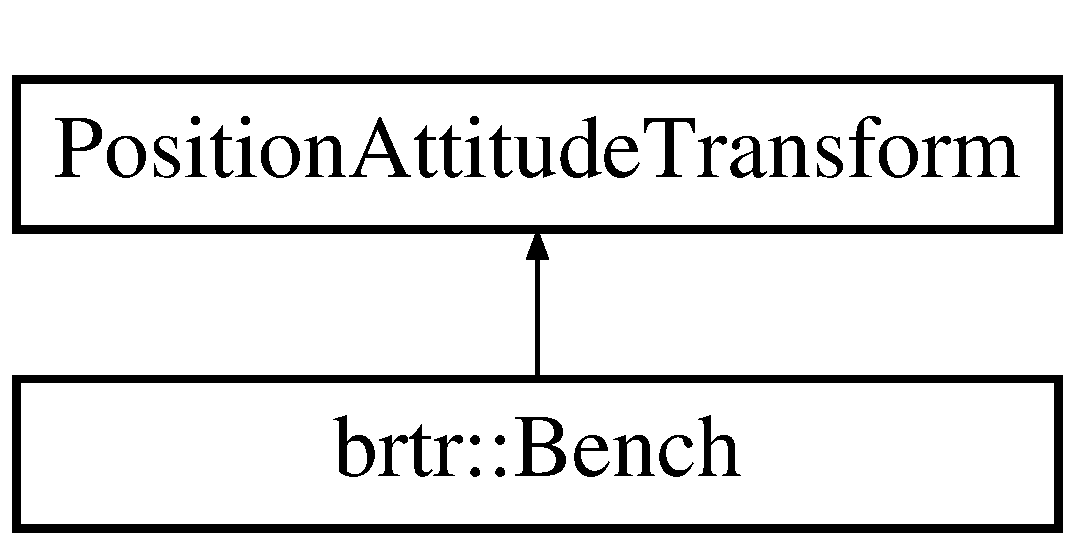
\includegraphics[height=2.000000cm]{classbrtr_1_1_bench}
\end{center}
\end{figure}
\subsection*{Public Member Functions}
\begin{DoxyCompactItemize}
\item 
\hyperlink{classbrtr_1_1_bench_a66ae6f45365c36daeabeed1a4b778d83}{Bench} (const Vec3 \&pcenter=Vec3(0, 0, 0), const double plength=8)
\item 
ref\+\_\+ptr\\*
$<$ Position\+Attitude\+Transform $>$ \hyperlink{classbrtr_1_1_bench_ad59e81ffbe90a7297bd5f256a54a234e}{get\+Hitbox} (const double alpha, double height=8)
\begin{DoxyCompactList}\small\item\em return the Hitbox of the \hyperlink{classbrtr_1_1_bench}{Bench} \end{DoxyCompactList}\item 
\hyperlink{classbrtr_1_1_bench_a9bd8ae1e6e48eb278206eff7102cac23}{Bench} (const \hyperlink{classbrtr_1_1_bench}{Bench} \&, const Copy\+Op \&copyop=Copy\+Op\+::\+S\+H\+A\+L\+L\+O\+W\+\_\+\+C\+O\+P\+Y)
\item 
\hyperlink{classbrtr_1_1_bench_a22ffdb328f6dac6737108d0f7aa34f67}{$\sim$\+Bench} ()
\end{DoxyCompactItemize}
\subsection*{Private Member Functions}
\begin{DoxyCompactItemize}
\item 
void \hyperlink{classbrtr_1_1_bench_a2813d4878b8a5ef09219323b2f6c9cf5}{init\+Bench} (const double plength)
\begin{DoxyCompactList}\small\item\em initialize the bench \end{DoxyCompactList}\item 
ref\+\_\+ptr$<$ Material $>$ \hyperlink{classbrtr_1_1_bench_aafa199aa2218d57b290d99843a1443d4}{create\+Iron\+Material} ()
\begin{DoxyCompactList}\small\item\em create the material for iron objects \end{DoxyCompactList}\item 
ref\+\_\+ptr$<$ Material $>$ \hyperlink{classbrtr_1_1_bench_a57d6d3f038d3f0e8d5f8b83895a6670a}{create\+Wood\+Material} ()
\begin{DoxyCompactList}\small\item\em create the material for wood objects \end{DoxyCompactList}\item 
ref\+\_\+ptr$<$ Group $>$ \hyperlink{classbrtr_1_1_bench_aefe5a9043a63e13d83c31a42046c6912}{create\+Leg} ()
\item 
ref\+\_\+ptr$<$ Group $>$ \hyperlink{classbrtr_1_1_bench_ae17e8e692f6c6deb7b722b5df58dc04b}{create\+Bar} ()
\item 
ref\+\_\+ptr$<$ Group $>$ \hyperlink{classbrtr_1_1_bench_a0547e73d10f329b2a9b4453b6319f472}{create\+Seat} (const double width)
\begin{DoxyCompactList}\small\item\em creates the seat \end{DoxyCompactList}\item 
ref\+\_\+ptr$<$ Group $>$ \hyperlink{classbrtr_1_1_bench_a9956994e6a20cbbd0f0ce9eb6df25917}{create\+Armrest} (double radius, double width, double \hyperlink{classbrtr_1_1_bench_a81188a60871201d741c288396430964d}{length}, double totalwidth)
\begin{DoxyCompactList}\small\item\em creates the armrest \end{DoxyCompactList}\item 
ref\+\_\+ptr$<$ Geometry $>$ \hyperlink{classbrtr_1_1_bench_a28443b856188050680a2c0ab4ad31a93}{create\+Armrest\+Sides\+Front\+Back} (double radius, double width, int lsteps, int wsteps, bool flip=true)
\begin{DoxyCompactList}\small\item\em creates the front/back for the armrest \end{DoxyCompactList}\item 
ref\+\_\+ptr$<$ Geometry $>$ \hyperlink{classbrtr_1_1_bench_afac56bea39f6e5e72140d4512dd711d3}{create\+Armrest\+Sides\+Left\+Right} (double \hyperlink{classbrtr_1_1_bench_a81188a60871201d741c288396430964d}{length}, double width, int lsteps, int wsteps, bool flip=true)
\begin{DoxyCompactList}\small\item\em creates the left/rigth for the armrest \end{DoxyCompactList}\item 
ref\+\_\+ptr$<$ Draw\+Elements\+U\+Int $>$ \hyperlink{classbrtr_1_1_bench_a90c4ae616eb8d7bf669af2983ed3cd1d}{get\+Primitive\+Setfor\+A\+Rectangle} (int lsteps, int wsteps)
\begin{DoxyCompactList}\small\item\em creates a primitives set for the get\+Rectangle function \end{DoxyCompactList}\end{DoxyCompactItemize}
\subsection*{Private Attributes}
\begin{DoxyCompactItemize}
\item 
Vec3 \hyperlink{classbrtr_1_1_bench_a5ea108ad6ee96d487ac00ecacc383aa2}{center}
\item 
double \hyperlink{classbrtr_1_1_bench_a81188a60871201d741c288396430964d}{length}
\item 
ref\+\_\+ptr$<$ Group $>$ \hyperlink{classbrtr_1_1_bench_aa3da8798872d1c2d595c24a48a5cb427}{bench}
\end{DoxyCompactItemize}


\subsection{Detailed Description}
\hyperlink{classbrtr_1_1_bench}{Bench} class, creates a bench Object. 

creates a bench with a given length at a given position. The length has to be between 2 and 30 \begin{DoxyAuthor}{Author}
Marcel Felix 
\end{DoxyAuthor}
\begin{DoxyVersion}{Version}
1.\+0 
\end{DoxyVersion}
\begin{DoxyDate}{Date}
2014
\end{DoxyDate}
\begin{DoxyCopyright}{Copyright}
G\+N\+U Public License. 
\end{DoxyCopyright}


Definition at line \hyperlink{_bench_8h_source_l00024}{24} of file \hyperlink{_bench_8h_source}{Bench.\+h}.



\subsection{Constructor \& Destructor Documentation}
\hypertarget{classbrtr_1_1_bench_a66ae6f45365c36daeabeed1a4b778d83}{\index{brtr\+::\+Bench@{brtr\+::\+Bench}!Bench@{Bench}}
\index{Bench@{Bench}!brtr\+::\+Bench@{brtr\+::\+Bench}}
\subsubsection[{Bench}]{\setlength{\rightskip}{0pt plus 5cm}brtr\+::\+Bench\+::\+Bench (
\begin{DoxyParamCaption}
\item[{const Vec3 \&}]{pcenter = {\ttfamily Vec3(0,~0,~0)}, }
\item[{const double}]{plength = {\ttfamily 8}}
\end{DoxyParamCaption}
)}}\label{classbrtr_1_1_bench_a66ae6f45365c36daeabeed1a4b778d83}


Definition at line \hyperlink{_bench_8cpp_source_l00007}{7} of file \hyperlink{_bench_8cpp_source}{Bench.\+cpp}.

\hypertarget{classbrtr_1_1_bench_a9bd8ae1e6e48eb278206eff7102cac23}{\index{brtr\+::\+Bench@{brtr\+::\+Bench}!Bench@{Bench}}
\index{Bench@{Bench}!brtr\+::\+Bench@{brtr\+::\+Bench}}
\subsubsection[{Bench}]{\setlength{\rightskip}{0pt plus 5cm}brtr\+::\+Bench\+::\+Bench (
\begin{DoxyParamCaption}
\item[{const {\bf Bench} \&}]{copy, }
\item[{const Copy\+Op \&}]{copyop = {\ttfamily CopyOp\+:\+:SHALLOW\+\_\+COPY}}
\end{DoxyParamCaption}
)}}\label{classbrtr_1_1_bench_a9bd8ae1e6e48eb278206eff7102cac23}


Definition at line \hyperlink{_bench_8cpp_source_l00018}{18} of file \hyperlink{_bench_8cpp_source}{Bench.\+cpp}.

\hypertarget{classbrtr_1_1_bench_a22ffdb328f6dac6737108d0f7aa34f67}{\index{brtr\+::\+Bench@{brtr\+::\+Bench}!````~Bench@{$\sim$\+Bench}}
\index{````~Bench@{$\sim$\+Bench}!brtr\+::\+Bench@{brtr\+::\+Bench}}
\subsubsection[{$\sim$\+Bench}]{\setlength{\rightskip}{0pt plus 5cm}brtr\+::\+Bench\+::$\sim$\+Bench (
\begin{DoxyParamCaption}
{}
\end{DoxyParamCaption}
)}}\label{classbrtr_1_1_bench_a22ffdb328f6dac6737108d0f7aa34f67}


Definition at line \hyperlink{_bench_8cpp_source_l00021}{21} of file \hyperlink{_bench_8cpp_source}{Bench.\+cpp}.



\subsection{Member Function Documentation}
\hypertarget{classbrtr_1_1_bench_a9956994e6a20cbbd0f0ce9eb6df25917}{\index{brtr\+::\+Bench@{brtr\+::\+Bench}!create\+Armrest@{create\+Armrest}}
\index{create\+Armrest@{create\+Armrest}!brtr\+::\+Bench@{brtr\+::\+Bench}}
\subsubsection[{create\+Armrest}]{\setlength{\rightskip}{0pt plus 5cm}ref\+\_\+ptr$<$ Group $>$ brtr\+::\+Bench\+::create\+Armrest (
\begin{DoxyParamCaption}
\item[{double}]{radius, }
\item[{double}]{width, }
\item[{double}]{length, }
\item[{double}]{totalwidth}
\end{DoxyParamCaption}
)\hspace{0.3cm}{\ttfamily [private]}}}\label{classbrtr_1_1_bench_a9956994e6a20cbbd0f0ce9eb6df25917}


creates the armrest 


\begin{DoxyParams}{Parameters}
{\em radius} & the distance between bench and armrest \\
\hline
{\em width} & width of the armrest \\
\hline
{\em length} & length of the armrest \\
\hline
{\em totalwidth} & width of the bar on the armrest \\
\hline
\end{DoxyParams}


Definition at line \hyperlink{_bench_8cpp_source_l00252}{252} of file \hyperlink{_bench_8cpp_source}{Bench.\+cpp}.

\hypertarget{classbrtr_1_1_bench_a28443b856188050680a2c0ab4ad31a93}{\index{brtr\+::\+Bench@{brtr\+::\+Bench}!create\+Armrest\+Sides\+Front\+Back@{create\+Armrest\+Sides\+Front\+Back}}
\index{create\+Armrest\+Sides\+Front\+Back@{create\+Armrest\+Sides\+Front\+Back}!brtr\+::\+Bench@{brtr\+::\+Bench}}
\subsubsection[{create\+Armrest\+Sides\+Front\+Back}]{\setlength{\rightskip}{0pt plus 5cm}ref\+\_\+ptr$<$ Geometry $>$ brtr\+::\+Bench\+::create\+Armrest\+Sides\+Front\+Back (
\begin{DoxyParamCaption}
\item[{double}]{radius, }
\item[{double}]{width, }
\item[{int}]{lsteps, }
\item[{int}]{wsteps, }
\item[{bool}]{flip = {\ttfamily true}}
\end{DoxyParamCaption}
)\hspace{0.3cm}{\ttfamily [private]}}}\label{classbrtr_1_1_bench_a28443b856188050680a2c0ab4ad31a93}


creates the front/back for the armrest 


\begin{DoxyParams}{Parameters}
{\em radius} & the distance between bench and armrest \\
\hline
{\em width} & width of the armrest \\
\hline
{\em length} & length of the armrest \\
\hline
{\em flip} & switch between front and back creation \\
\hline
\end{DoxyParams}


Definition at line \hyperlink{_bench_8cpp_source_l00140}{140} of file \hyperlink{_bench_8cpp_source}{Bench.\+cpp}.

\hypertarget{classbrtr_1_1_bench_afac56bea39f6e5e72140d4512dd711d3}{\index{brtr\+::\+Bench@{brtr\+::\+Bench}!create\+Armrest\+Sides\+Left\+Right@{create\+Armrest\+Sides\+Left\+Right}}
\index{create\+Armrest\+Sides\+Left\+Right@{create\+Armrest\+Sides\+Left\+Right}!brtr\+::\+Bench@{brtr\+::\+Bench}}
\subsubsection[{create\+Armrest\+Sides\+Left\+Right}]{\setlength{\rightskip}{0pt plus 5cm}ref\+\_\+ptr$<$ Geometry $>$ brtr\+::\+Bench\+::create\+Armrest\+Sides\+Left\+Right (
\begin{DoxyParamCaption}
\item[{double}]{length, }
\item[{double}]{width, }
\item[{int}]{lsteps, }
\item[{int}]{wsteps, }
\item[{bool}]{flip = {\ttfamily true}}
\end{DoxyParamCaption}
)\hspace{0.3cm}{\ttfamily [private]}}}\label{classbrtr_1_1_bench_afac56bea39f6e5e72140d4512dd711d3}


creates the left/rigth for the armrest 


\begin{DoxyParams}{Parameters}
{\em radius} & the distance between bench and armrest \\
\hline
{\em width} & width of the armrest \\
\hline
{\em length} & length of the armrest \\
\hline
{\em flip} & switch between front and back creation \\
\hline
\end{DoxyParams}


Definition at line \hyperlink{_bench_8cpp_source_l00084}{84} of file \hyperlink{_bench_8cpp_source}{Bench.\+cpp}.

\hypertarget{classbrtr_1_1_bench_ae17e8e692f6c6deb7b722b5df58dc04b}{\index{brtr\+::\+Bench@{brtr\+::\+Bench}!create\+Bar@{create\+Bar}}
\index{create\+Bar@{create\+Bar}!brtr\+::\+Bench@{brtr\+::\+Bench}}
\subsubsection[{create\+Bar}]{\setlength{\rightskip}{0pt plus 5cm}ref\+\_\+ptr$<$ Group $>$ brtr\+::\+Bench\+::create\+Bar (
\begin{DoxyParamCaption}
{}
\end{DoxyParamCaption}
)\hspace{0.3cm}{\ttfamily [private]}}}\label{classbrtr_1_1_bench_ae17e8e692f6c6deb7b722b5df58dc04b}


Definition at line \hyperlink{_bench_8cpp_source_l00331}{331} of file \hyperlink{_bench_8cpp_source}{Bench.\+cpp}.

\hypertarget{classbrtr_1_1_bench_aafa199aa2218d57b290d99843a1443d4}{\index{brtr\+::\+Bench@{brtr\+::\+Bench}!create\+Iron\+Material@{create\+Iron\+Material}}
\index{create\+Iron\+Material@{create\+Iron\+Material}!brtr\+::\+Bench@{brtr\+::\+Bench}}
\subsubsection[{create\+Iron\+Material}]{\setlength{\rightskip}{0pt plus 5cm}ref\+\_\+ptr$<$ Material $>$ brtr\+::\+Bench\+::create\+Iron\+Material (
\begin{DoxyParamCaption}
{}
\end{DoxyParamCaption}
)\hspace{0.3cm}{\ttfamily [private]}}}\label{classbrtr_1_1_bench_aafa199aa2218d57b290d99843a1443d4}


create the material for iron objects 



Definition at line \hyperlink{_bench_8cpp_source_l00053}{53} of file \hyperlink{_bench_8cpp_source}{Bench.\+cpp}.

\hypertarget{classbrtr_1_1_bench_aefe5a9043a63e13d83c31a42046c6912}{\index{brtr\+::\+Bench@{brtr\+::\+Bench}!create\+Leg@{create\+Leg}}
\index{create\+Leg@{create\+Leg}!brtr\+::\+Bench@{brtr\+::\+Bench}}
\subsubsection[{create\+Leg}]{\setlength{\rightskip}{0pt plus 5cm}ref\+\_\+ptr$<$ Group $>$ brtr\+::\+Bench\+::create\+Leg (
\begin{DoxyParamCaption}
{}
\end{DoxyParamCaption}
)\hspace{0.3cm}{\ttfamily [private]}}}\label{classbrtr_1_1_bench_aefe5a9043a63e13d83c31a42046c6912}


Definition at line \hyperlink{_bench_8cpp_source_l00190}{190} of file \hyperlink{_bench_8cpp_source}{Bench.\+cpp}.

\hypertarget{classbrtr_1_1_bench_a0547e73d10f329b2a9b4453b6319f472}{\index{brtr\+::\+Bench@{brtr\+::\+Bench}!create\+Seat@{create\+Seat}}
\index{create\+Seat@{create\+Seat}!brtr\+::\+Bench@{brtr\+::\+Bench}}
\subsubsection[{create\+Seat}]{\setlength{\rightskip}{0pt plus 5cm}ref\+\_\+ptr$<$ Group $>$ brtr\+::\+Bench\+::create\+Seat (
\begin{DoxyParamCaption}
\item[{const double}]{width}
\end{DoxyParamCaption}
)\hspace{0.3cm}{\ttfamily [private]}}}\label{classbrtr_1_1_bench_a0547e73d10f329b2a9b4453b6319f472}


creates the seat 


\begin{DoxyParams}{Parameters}
{\em width} & the width/length of the Seat \\
\hline
\end{DoxyParams}


Definition at line \hyperlink{_bench_8cpp_source_l00212}{212} of file \hyperlink{_bench_8cpp_source}{Bench.\+cpp}.

\hypertarget{classbrtr_1_1_bench_a57d6d3f038d3f0e8d5f8b83895a6670a}{\index{brtr\+::\+Bench@{brtr\+::\+Bench}!create\+Wood\+Material@{create\+Wood\+Material}}
\index{create\+Wood\+Material@{create\+Wood\+Material}!brtr\+::\+Bench@{brtr\+::\+Bench}}
\subsubsection[{create\+Wood\+Material}]{\setlength{\rightskip}{0pt plus 5cm}ref\+\_\+ptr$<$ Material $>$ brtr\+::\+Bench\+::create\+Wood\+Material (
\begin{DoxyParamCaption}
{}
\end{DoxyParamCaption}
)\hspace{0.3cm}{\ttfamily [private]}}}\label{classbrtr_1_1_bench_a57d6d3f038d3f0e8d5f8b83895a6670a}


create the material for wood objects 



Definition at line \hyperlink{_bench_8cpp_source_l00062}{62} of file \hyperlink{_bench_8cpp_source}{Bench.\+cpp}.

\hypertarget{classbrtr_1_1_bench_ad59e81ffbe90a7297bd5f256a54a234e}{\index{brtr\+::\+Bench@{brtr\+::\+Bench}!get\+Hitbox@{get\+Hitbox}}
\index{get\+Hitbox@{get\+Hitbox}!brtr\+::\+Bench@{brtr\+::\+Bench}}
\subsubsection[{get\+Hitbox}]{\setlength{\rightskip}{0pt plus 5cm}ref\+\_\+ptr$<$ Position\+Attitude\+Transform $>$ brtr\+::\+Bench\+::get\+Hitbox (
\begin{DoxyParamCaption}
\item[{const double}]{alpha, }
\item[{double}]{height = {\ttfamily 8}}
\end{DoxyParamCaption}
)}}\label{classbrtr_1_1_bench_ad59e81ffbe90a7297bd5f256a54a234e}


return the Hitbox of the \hyperlink{classbrtr_1_1_bench}{Bench} 


\begin{DoxyParams}{Parameters}
{\em alpha} & \\
\hline
{\em height} & the height of the hitbox. height $<$ 0 will use the height of the bench \\
\hline
\end{DoxyParams}
\begin{DoxyReturn}{Returns}
the hitbox as a Position\+Attitude\+Transform with the given alpha value 
\end{DoxyReturn}


Definition at line \hyperlink{_bench_8cpp_source_l00024}{24} of file \hyperlink{_bench_8cpp_source}{Bench.\+cpp}.

\hypertarget{classbrtr_1_1_bench_a90c4ae616eb8d7bf669af2983ed3cd1d}{\index{brtr\+::\+Bench@{brtr\+::\+Bench}!get\+Primitive\+Setfor\+A\+Rectangle@{get\+Primitive\+Setfor\+A\+Rectangle}}
\index{get\+Primitive\+Setfor\+A\+Rectangle@{get\+Primitive\+Setfor\+A\+Rectangle}!brtr\+::\+Bench@{brtr\+::\+Bench}}
\subsubsection[{get\+Primitive\+Setfor\+A\+Rectangle}]{\setlength{\rightskip}{0pt plus 5cm}ref\+\_\+ptr$<$ Draw\+Elements\+U\+Int $>$ brtr\+::\+Bench\+::get\+Primitive\+Setfor\+A\+Rectangle (
\begin{DoxyParamCaption}
\item[{int}]{lsteps, }
\item[{int}]{wsteps}
\end{DoxyParamCaption}
)\hspace{0.3cm}{\ttfamily [private]}}}\label{classbrtr_1_1_bench_a90c4ae616eb8d7bf669af2983ed3cd1d}


creates a primitives set for the get\+Rectangle function 

parts of the function are copy/pasted from Chapter 7, C\+G1 Lecture Script by Frauke Sprengel


\begin{DoxyParams}{Parameters}
{\em lsteps} & \\
\hline
{\em wsteps} & \\
\hline
\end{DoxyParams}
\begin{DoxyReturn}{Returns}
a ref\+\_\+ptr$<$\+Draw\+Elements\+U\+Int$>$ containing the primitives set 
\end{DoxyReturn}


Definition at line \hyperlink{_bench_8cpp_source_l00071}{71} of file \hyperlink{_bench_8cpp_source}{Bench.\+cpp}.

\hypertarget{classbrtr_1_1_bench_a2813d4878b8a5ef09219323b2f6c9cf5}{\index{brtr\+::\+Bench@{brtr\+::\+Bench}!init\+Bench@{init\+Bench}}
\index{init\+Bench@{init\+Bench}!brtr\+::\+Bench@{brtr\+::\+Bench}}
\subsubsection[{init\+Bench}]{\setlength{\rightskip}{0pt plus 5cm}void brtr\+::\+Bench\+::init\+Bench (
\begin{DoxyParamCaption}
\item[{const double}]{plength}
\end{DoxyParamCaption}
)\hspace{0.3cm}{\ttfamily [private]}}}\label{classbrtr_1_1_bench_a2813d4878b8a5ef09219323b2f6c9cf5}


initialize the bench 


\begin{DoxyParams}{Parameters}
{\em plength} & the length of the bench \\
\hline
\end{DoxyParams}


Definition at line \hyperlink{_bench_8cpp_source_l00360}{360} of file \hyperlink{_bench_8cpp_source}{Bench.\+cpp}.



\subsection{Member Data Documentation}
\hypertarget{classbrtr_1_1_bench_aa3da8798872d1c2d595c24a48a5cb427}{\index{brtr\+::\+Bench@{brtr\+::\+Bench}!bench@{bench}}
\index{bench@{bench}!brtr\+::\+Bench@{brtr\+::\+Bench}}
\subsubsection[{bench}]{\setlength{\rightskip}{0pt plus 5cm}ref\+\_\+ptr$<$Group$>$ brtr\+::\+Bench\+::bench\hspace{0.3cm}{\ttfamily [private]}}}\label{classbrtr_1_1_bench_aa3da8798872d1c2d595c24a48a5cb427}


Definition at line \hyperlink{_bench_8h_source_l00108}{108} of file \hyperlink{_bench_8h_source}{Bench.\+h}.

\hypertarget{classbrtr_1_1_bench_a5ea108ad6ee96d487ac00ecacc383aa2}{\index{brtr\+::\+Bench@{brtr\+::\+Bench}!center@{center}}
\index{center@{center}!brtr\+::\+Bench@{brtr\+::\+Bench}}
\subsubsection[{center}]{\setlength{\rightskip}{0pt plus 5cm}Vec3 brtr\+::\+Bench\+::center\hspace{0.3cm}{\ttfamily [private]}}}\label{classbrtr_1_1_bench_a5ea108ad6ee96d487ac00ecacc383aa2}


Definition at line \hyperlink{_bench_8h_source_l00105}{105} of file \hyperlink{_bench_8h_source}{Bench.\+h}.

\hypertarget{classbrtr_1_1_bench_a81188a60871201d741c288396430964d}{\index{brtr\+::\+Bench@{brtr\+::\+Bench}!length@{length}}
\index{length@{length}!brtr\+::\+Bench@{brtr\+::\+Bench}}
\subsubsection[{length}]{\setlength{\rightskip}{0pt plus 5cm}double brtr\+::\+Bench\+::length\hspace{0.3cm}{\ttfamily [private]}}}\label{classbrtr_1_1_bench_a81188a60871201d741c288396430964d}


Definition at line \hyperlink{_bench_8h_source_l00107}{107} of file \hyperlink{_bench_8h_source}{Bench.\+h}.



The documentation for this class was generated from the following files\+:\begin{DoxyCompactItemize}
\item 
header/\hyperlink{_bench_8h}{Bench.\+h}\item 
Objects/\hyperlink{_bench_8cpp}{Bench.\+cpp}\end{DoxyCompactItemize}

\hypertarget{structbrtr_1_1_body_of_rotation_function}{\section{brtr\+:\+:Body\+Of\+Rotation\+Function Struct Reference}
\label{structbrtr_1_1_body_of_rotation_function}\index{brtr\+::\+Body\+Of\+Rotation\+Function@{brtr\+::\+Body\+Of\+Rotation\+Function}}
}


struct holding the function, which calculates the radius in dependece of the height. lambda (double)-\/$>$double func, int end, Body\+Of\+Rotation\+Function$\ast$ next\+Func if one wish to have more then one function then the end value and next\+Func pointer must be set accordingly the end+1 is the beginning x of the next function  




{\ttfamily \#include $<$Util\+Functions.\+h$>$}

\subsection*{Public Member Functions}
\begin{DoxyCompactItemize}
\item 
double \hyperlink{structbrtr_1_1_body_of_rotation_function_a22861c378686dabe1c35c90a0a8dcf46}{derivation} (double x) const 
\end{DoxyCompactItemize}
\subsection*{Public Attributes}
\begin{DoxyCompactItemize}
\item 
std\+::function$<$ double(double)$>$ \hyperlink{structbrtr_1_1_body_of_rotation_function_a5fda598eb0a63696b059e3a27c01142b}{func}
\begin{DoxyCompactList}\small\item\em the function \end{DoxyCompactList}\item 
double \hyperlink{structbrtr_1_1_body_of_rotation_function_a46667ab72bfeddc305bf31fa359c8699}{end}
\begin{DoxyCompactList}\small\item\em the end value of the function, should be less or equal create\+Body\+Of\+Rotation\+::height \end{DoxyCompactList}\item 
const \hyperlink{structbrtr_1_1_body_of_rotation_function}{Body\+Of\+Rotation\+Function} $\ast$ \hyperlink{structbrtr_1_1_body_of_rotation_function_ad7df29eaeb2504928488691196cc06eb}{next\+Func}
\begin{DoxyCompactList}\small\item\em if end is less then create\+Body\+Of\+Rotation\+::height, must point towards the next function which shall be used from end \end{DoxyCompactList}\end{DoxyCompactItemize}


\subsection{Detailed Description}
struct holding the function, which calculates the radius in dependece of the height. lambda (double)-\/$>$double func, int end, Body\+Of\+Rotation\+Function$\ast$ next\+Func if one wish to have more then one function then the end value and next\+Func pointer must be set accordingly the end+1 is the beginning x of the next function 

Definition at line \hyperlink{_util_functions_8h_source_l00040}{40} of file \hyperlink{_util_functions_8h_source}{Util\+Functions.\+h}.



\subsection{Member Function Documentation}
\hypertarget{structbrtr_1_1_body_of_rotation_function_a22861c378686dabe1c35c90a0a8dcf46}{\index{brtr\+::\+Body\+Of\+Rotation\+Function@{brtr\+::\+Body\+Of\+Rotation\+Function}!derivation@{derivation}}
\index{derivation@{derivation}!brtr\+::\+Body\+Of\+Rotation\+Function@{brtr\+::\+Body\+Of\+Rotation\+Function}}
\subsubsection[{derivation}]{\setlength{\rightskip}{0pt plus 5cm}double brtr\+::\+Body\+Of\+Rotation\+Function\+::derivation (
\begin{DoxyParamCaption}
\item[{double}]{x}
\end{DoxyParamCaption}
) const\hspace{0.3cm}{\ttfamily [inline]}}}\label{structbrtr_1_1_body_of_rotation_function_a22861c378686dabe1c35c90a0a8dcf46}


Definition at line \hyperlink{_util_functions_8h_source_l00044}{44} of file \hyperlink{_util_functions_8h_source}{Util\+Functions.\+h}.



\subsection{Member Data Documentation}
\hypertarget{structbrtr_1_1_body_of_rotation_function_a46667ab72bfeddc305bf31fa359c8699}{\index{brtr\+::\+Body\+Of\+Rotation\+Function@{brtr\+::\+Body\+Of\+Rotation\+Function}!end@{end}}
\index{end@{end}!brtr\+::\+Body\+Of\+Rotation\+Function@{brtr\+::\+Body\+Of\+Rotation\+Function}}
\subsubsection[{end}]{\setlength{\rightskip}{0pt plus 5cm}double brtr\+::\+Body\+Of\+Rotation\+Function\+::end}}\label{structbrtr_1_1_body_of_rotation_function_a46667ab72bfeddc305bf31fa359c8699}


the end value of the function, should be less or equal create\+Body\+Of\+Rotation\+::height 



Definition at line \hyperlink{_util_functions_8h_source_l00042}{42} of file \hyperlink{_util_functions_8h_source}{Util\+Functions.\+h}.

\hypertarget{structbrtr_1_1_body_of_rotation_function_a5fda598eb0a63696b059e3a27c01142b}{\index{brtr\+::\+Body\+Of\+Rotation\+Function@{brtr\+::\+Body\+Of\+Rotation\+Function}!func@{func}}
\index{func@{func}!brtr\+::\+Body\+Of\+Rotation\+Function@{brtr\+::\+Body\+Of\+Rotation\+Function}}
\subsubsection[{func}]{\setlength{\rightskip}{0pt plus 5cm}std\+::function$<$double(double)$>$ brtr\+::\+Body\+Of\+Rotation\+Function\+::func}}\label{structbrtr_1_1_body_of_rotation_function_a5fda598eb0a63696b059e3a27c01142b}


the function 



Definition at line \hyperlink{_util_functions_8h_source_l00041}{41} of file \hyperlink{_util_functions_8h_source}{Util\+Functions.\+h}.

\hypertarget{structbrtr_1_1_body_of_rotation_function_ad7df29eaeb2504928488691196cc06eb}{\index{brtr\+::\+Body\+Of\+Rotation\+Function@{brtr\+::\+Body\+Of\+Rotation\+Function}!next\+Func@{next\+Func}}
\index{next\+Func@{next\+Func}!brtr\+::\+Body\+Of\+Rotation\+Function@{brtr\+::\+Body\+Of\+Rotation\+Function}}
\subsubsection[{next\+Func}]{\setlength{\rightskip}{0pt plus 5cm}const {\bf Body\+Of\+Rotation\+Function}$\ast$ brtr\+::\+Body\+Of\+Rotation\+Function\+::next\+Func}}\label{structbrtr_1_1_body_of_rotation_function_ad7df29eaeb2504928488691196cc06eb}


if end is less then create\+Body\+Of\+Rotation\+::height, must point towards the next function which shall be used from end 



Definition at line \hyperlink{_util_functions_8h_source_l00043}{43} of file \hyperlink{_util_functions_8h_source}{Util\+Functions.\+h}.



The documentation for this struct was generated from the following file\+:\begin{DoxyCompactItemize}
\item 
header/\hyperlink{_util_functions_8h}{Util\+Functions.\+h}\end{DoxyCompactItemize}

\hypertarget{classbrtr_1_1_cel_shading}{\section{brtr\+:\+:Cel\+Shading Class Reference}
\label{classbrtr_1_1_cel_shading}\index{brtr\+::\+Cel\+Shading@{brtr\+::\+Cel\+Shading}}
}


Cel\+Sading Effect, every child of this node will get the effect.  




{\ttfamily \#include $<$Cel\+Shading.\+h$>$}

Inheritance diagram for brtr\+:\+:Cel\+Shading\+:\begin{figure}[H]
\begin{center}
\leavevmode
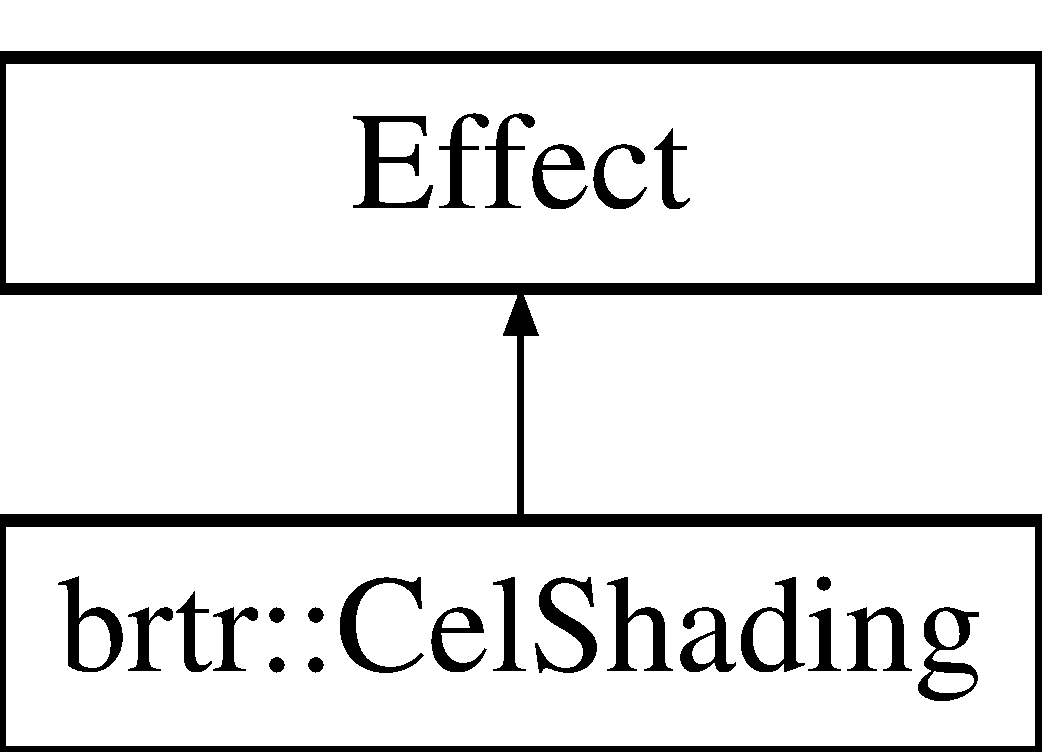
\includegraphics[height=2.000000cm]{classbrtr_1_1_cel_shading}
\end{center}
\end{figure}
\subsection*{Public Member Functions}
\begin{DoxyCompactItemize}
\item 
\hyperlink{classbrtr_1_1_cel_shading_ae497a14c2c379b608643d8f39d156b52}{Cel\+Shading} (bool second\+Pass=true, std\+::string vert\+Source=\char`\"{}cel\+Shader.\+vert\char`\"{})
\begin{DoxyCompactList}\small\item\em Constructor. \end{DoxyCompactList}\item 
\hyperlink{classbrtr_1_1_cel_shading_affb65fcbb6ffe405f60b840c52cdc26c}{Cel\+Shading} (const \hyperlink{classbrtr_1_1_cel_shading}{Cel\+Shading} \&copy, const osg\+::\+Copy\+Op \&copyop=osg\+::\+Copy\+Op\+::\+S\+H\+A\+L\+L\+O\+W\+\_\+\+C\+O\+P\+Y)
\item 
\hyperlink{classbrtr_1_1_cel_shading_a02ab424cf06935b9560b5c39d733d02c}{M\+E\+T\+A\+\_\+\+Effect} (null, \hyperlink{classbrtr_1_1_cel_shading}{Cel\+Shading},\char`\"{}Cel\+Shading\char`\"{},\char`\"{}This effect implements a technique called 'Cel-\/Shading' to produce a \char`\"{}\char`\"{}cartoon-\/style (non photorealistic) rendering. Two passes are required\+: \char`\"{}\char`\"{}the first one draws solid surfaces, the second one draws the outlines. \char`\"{}\char`\"{}Vertices Shader, Toon Texture pass can be customize upon creating.\char`\"{},\char`\"{}Marco Jez; O\+G\+L\+S\+L port by Mike Weiblen, adaptions by Gleb Ostrowski \char`\"{})
\end{DoxyCompactItemize}
\subsection*{Protected Member Functions}
\begin{DoxyCompactItemize}
\item 
virtual \hyperlink{classbrtr_1_1_cel_shading_ab6148e389081719d56d2971cc8924841}{$\sim$\+Cel\+Shading} ()
\item 
bool \hyperlink{classbrtr_1_1_cel_shading_a28212bb66f29ff8cf1169625b598b93b}{define\+\_\+techniques} ()
\end{DoxyCompactItemize}
\subsection*{Private Attributes}
\begin{DoxyCompactItemize}
\item 
osg\+::ref\+\_\+ptr$<$ osg\+::\+Material $>$ \hyperlink{classbrtr_1_1_cel_shading_ae67a870d7a985694fb0d3290f0163f84}{\+\_\+material}
\item 
osg\+::ref\+\_\+ptr$<$ osg\+::\+Line\+Width $>$ \hyperlink{classbrtr_1_1_cel_shading_ae1e0a4de3ca638da0fe0a3b3aa018f07}{\+\_\+line\+Width}
\item 
bool \hyperlink{classbrtr_1_1_cel_shading_a15226eda13f5a3deaee3260414f664bf}{\+\_\+second\+Pass}
\item 
std\+::string \hyperlink{classbrtr_1_1_cel_shading_a6c9ea02f1a90b0ba711394c4ff716081}{\+\_\+vert\+Source}
\end{DoxyCompactItemize}


\subsection{Detailed Description}
Cel\+Sading Effect, every child of this node will get the effect. 

This effect implements a technique called 'Cel-\/\+Shading' to produce a cartoon-\/style (non photorealistic) rendering.~\newline
 Two passes are required\+:~\newline
 the first one draws solid surfaces, the second one draws the outlines. \begin{DoxyAuthor}{Author}
Gleb Ostrowski 
\end{DoxyAuthor}
\begin{DoxyVersion}{Version}
1.\+0 
\end{DoxyVersion}
\begin{DoxyDate}{Date}
2014 
\end{DoxyDate}
\begin{DoxyPrecond}{Precondition}
In Texture Layer 1 (stateset) must be the Toon\+Texture set 
\end{DoxyPrecond}
\begin{DoxyCopyright}{Copyright}
G\+N\+U Public License. 
\end{DoxyCopyright}


Definition at line \hyperlink{_cel_shading_8h_source_l00018}{18} of file \hyperlink{_cel_shading_8h_source}{Cel\+Shading.\+h}.



\subsection{Constructor \& Destructor Documentation}
\hypertarget{classbrtr_1_1_cel_shading_ae497a14c2c379b608643d8f39d156b52}{\index{brtr\+::\+Cel\+Shading@{brtr\+::\+Cel\+Shading}!Cel\+Shading@{Cel\+Shading}}
\index{Cel\+Shading@{Cel\+Shading}!brtr\+::\+Cel\+Shading@{brtr\+::\+Cel\+Shading}}
\subsubsection[{Cel\+Shading}]{\setlength{\rightskip}{0pt plus 5cm}brtr\+::\+Cel\+Shading\+::\+Cel\+Shading (
\begin{DoxyParamCaption}
\item[{bool}]{second\+Pass = {\ttfamily true}, }
\item[{std\+::string}]{vert\+Source = {\ttfamily \char`\"{}celShader.vert\char`\"{}}}
\end{DoxyParamCaption}
)}}\label{classbrtr_1_1_cel_shading_ae497a14c2c379b608643d8f39d156b52}


Constructor. 


\begin{DoxyParams}{Parameters}
{\em second\+Pass} & if false, no outlines are being drawn \\
\hline
{\em vert\+Source} & one can set explicitly the vertex shader \\
\hline
\end{DoxyParams}


Definition at line \hyperlink{_cel_shading_8cpp_source_l00097}{97} of file \hyperlink{_cel_shading_8cpp_source}{Cel\+Shading.\+cpp}.

\hypertarget{classbrtr_1_1_cel_shading_affb65fcbb6ffe405f60b840c52cdc26c}{\index{brtr\+::\+Cel\+Shading@{brtr\+::\+Cel\+Shading}!Cel\+Shading@{Cel\+Shading}}
\index{Cel\+Shading@{Cel\+Shading}!brtr\+::\+Cel\+Shading@{brtr\+::\+Cel\+Shading}}
\subsubsection[{Cel\+Shading}]{\setlength{\rightskip}{0pt plus 5cm}brtr\+::\+Cel\+Shading\+::\+Cel\+Shading (
\begin{DoxyParamCaption}
\item[{const {\bf Cel\+Shading} \&}]{copy, }
\item[{const osg\+::\+Copy\+Op \&}]{copyop = {\ttfamily osg\+:\+:CopyOp\+:\+:SHALLOW\+\_\+COPY}}
\end{DoxyParamCaption}
)}}\label{classbrtr_1_1_cel_shading_affb65fcbb6ffe405f60b840c52cdc26c}


Definition at line \hyperlink{_cel_shading_8cpp_source_l00104}{104} of file \hyperlink{_cel_shading_8cpp_source}{Cel\+Shading.\+cpp}.

\hypertarget{classbrtr_1_1_cel_shading_ab6148e389081719d56d2971cc8924841}{\index{brtr\+::\+Cel\+Shading@{brtr\+::\+Cel\+Shading}!````~Cel\+Shading@{$\sim$\+Cel\+Shading}}
\index{````~Cel\+Shading@{$\sim$\+Cel\+Shading}!brtr\+::\+Cel\+Shading@{brtr\+::\+Cel\+Shading}}
\subsubsection[{$\sim$\+Cel\+Shading}]{\setlength{\rightskip}{0pt plus 5cm}virtual brtr\+::\+Cel\+Shading\+::$\sim$\+Cel\+Shading (
\begin{DoxyParamCaption}
{}
\end{DoxyParamCaption}
)\hspace{0.3cm}{\ttfamily [inline]}, {\ttfamily [protected]}, {\ttfamily [virtual]}}}\label{classbrtr_1_1_cel_shading_ab6148e389081719d56d2971cc8924841}


Definition at line \hyperlink{_cel_shading_8h_source_l00043}{43} of file \hyperlink{_cel_shading_8h_source}{Cel\+Shading.\+h}.



\subsection{Member Function Documentation}
\hypertarget{classbrtr_1_1_cel_shading_a28212bb66f29ff8cf1169625b598b93b}{\index{brtr\+::\+Cel\+Shading@{brtr\+::\+Cel\+Shading}!define\+\_\+techniques@{define\+\_\+techniques}}
\index{define\+\_\+techniques@{define\+\_\+techniques}!brtr\+::\+Cel\+Shading@{brtr\+::\+Cel\+Shading}}
\subsubsection[{define\+\_\+techniques}]{\setlength{\rightskip}{0pt plus 5cm}bool brtr\+::\+Cel\+Shading\+::define\+\_\+techniques (
\begin{DoxyParamCaption}
{}
\end{DoxyParamCaption}
)\hspace{0.3cm}{\ttfamily [protected]}}}\label{classbrtr_1_1_cel_shading_a28212bb66f29ff8cf1169625b598b93b}


Definition at line \hyperlink{_cel_shading_8cpp_source_l00110}{110} of file \hyperlink{_cel_shading_8cpp_source}{Cel\+Shading.\+cpp}.

\hypertarget{classbrtr_1_1_cel_shading_a02ab424cf06935b9560b5c39d733d02c}{\index{brtr\+::\+Cel\+Shading@{brtr\+::\+Cel\+Shading}!M\+E\+T\+A\+\_\+\+Effect@{M\+E\+T\+A\+\_\+\+Effect}}
\index{M\+E\+T\+A\+\_\+\+Effect@{M\+E\+T\+A\+\_\+\+Effect}!brtr\+::\+Cel\+Shading@{brtr\+::\+Cel\+Shading}}
\subsubsection[{M\+E\+T\+A\+\_\+\+Effect}]{\setlength{\rightskip}{0pt plus 5cm}brtr\+::\+Cel\+Shading\+::\+M\+E\+T\+A\+\_\+\+Effect (
\begin{DoxyParamCaption}
\item[{null}]{, }
\item[{{\bf Cel\+Shading}}]{, }
\item[{\char`\"{}Cel\+Shading\char`\"{}}]{, }
\item[{\char`\"{}This effect implements a technique called 'Cel-\/Shading' to produce a \char`\"{}\char`\"{}cartoon-\/style (non photorealistic) rendering. Two passes are required\+: \char`\"{}\char`\"{}the first one draws solid}]{surfaces, }
\item[{the second one draws the outlines.\char`\"{}\char`\"{}Vertices}]{Shader, }
\item[{Toon Texture pass can be customize upon creating.\char`\"{}}]{, }
\item[{\char`\"{}Marco Jez; O\+G\+L\+S\+L port by Mike}]{Weiblen, }
\item[{adaptions by Gleb Ostrowski\char`\"{}}]{}
\end{DoxyParamCaption}
)}}\label{classbrtr_1_1_cel_shading_a02ab424cf06935b9560b5c39d733d02c}


\subsection{Member Data Documentation}
\hypertarget{classbrtr_1_1_cel_shading_ae1e0a4de3ca638da0fe0a3b3aa018f07}{\index{brtr\+::\+Cel\+Shading@{brtr\+::\+Cel\+Shading}!\+\_\+line\+Width@{\+\_\+line\+Width}}
\index{\+\_\+line\+Width@{\+\_\+line\+Width}!brtr\+::\+Cel\+Shading@{brtr\+::\+Cel\+Shading}}
\subsubsection[{\+\_\+line\+Width}]{\setlength{\rightskip}{0pt plus 5cm}osg\+::ref\+\_\+ptr$<$osg\+::\+Line\+Width$>$ brtr\+::\+Cel\+Shading\+::\+\_\+line\+Width\hspace{0.3cm}{\ttfamily [private]}}}\label{classbrtr_1_1_cel_shading_ae1e0a4de3ca638da0fe0a3b3aa018f07}


Definition at line \hyperlink{_cel_shading_8h_source_l00049}{49} of file \hyperlink{_cel_shading_8h_source}{Cel\+Shading.\+h}.

\hypertarget{classbrtr_1_1_cel_shading_ae67a870d7a985694fb0d3290f0163f84}{\index{brtr\+::\+Cel\+Shading@{brtr\+::\+Cel\+Shading}!\+\_\+material@{\+\_\+material}}
\index{\+\_\+material@{\+\_\+material}!brtr\+::\+Cel\+Shading@{brtr\+::\+Cel\+Shading}}
\subsubsection[{\+\_\+material}]{\setlength{\rightskip}{0pt plus 5cm}osg\+::ref\+\_\+ptr$<$osg\+::\+Material$>$ brtr\+::\+Cel\+Shading\+::\+\_\+material\hspace{0.3cm}{\ttfamily [private]}}}\label{classbrtr_1_1_cel_shading_ae67a870d7a985694fb0d3290f0163f84}


Definition at line \hyperlink{_cel_shading_8h_source_l00048}{48} of file \hyperlink{_cel_shading_8h_source}{Cel\+Shading.\+h}.

\hypertarget{classbrtr_1_1_cel_shading_a15226eda13f5a3deaee3260414f664bf}{\index{brtr\+::\+Cel\+Shading@{brtr\+::\+Cel\+Shading}!\+\_\+second\+Pass@{\+\_\+second\+Pass}}
\index{\+\_\+second\+Pass@{\+\_\+second\+Pass}!brtr\+::\+Cel\+Shading@{brtr\+::\+Cel\+Shading}}
\subsubsection[{\+\_\+second\+Pass}]{\setlength{\rightskip}{0pt plus 5cm}bool brtr\+::\+Cel\+Shading\+::\+\_\+second\+Pass\hspace{0.3cm}{\ttfamily [private]}}}\label{classbrtr_1_1_cel_shading_a15226eda13f5a3deaee3260414f664bf}


Definition at line \hyperlink{_cel_shading_8h_source_l00050}{50} of file \hyperlink{_cel_shading_8h_source}{Cel\+Shading.\+h}.

\hypertarget{classbrtr_1_1_cel_shading_a6c9ea02f1a90b0ba711394c4ff716081}{\index{brtr\+::\+Cel\+Shading@{brtr\+::\+Cel\+Shading}!\+\_\+vert\+Source@{\+\_\+vert\+Source}}
\index{\+\_\+vert\+Source@{\+\_\+vert\+Source}!brtr\+::\+Cel\+Shading@{brtr\+::\+Cel\+Shading}}
\subsubsection[{\+\_\+vert\+Source}]{\setlength{\rightskip}{0pt plus 5cm}std\+::string brtr\+::\+Cel\+Shading\+::\+\_\+vert\+Source\hspace{0.3cm}{\ttfamily [private]}}}\label{classbrtr_1_1_cel_shading_a6c9ea02f1a90b0ba711394c4ff716081}


Definition at line \hyperlink{_cel_shading_8h_source_l00051}{51} of file \hyperlink{_cel_shading_8h_source}{Cel\+Shading.\+h}.



The documentation for this class was generated from the following files\+:\begin{DoxyCompactItemize}
\item 
header/\hyperlink{_cel_shading_8h}{Cel\+Shading.\+h}\item 
Shader/\hyperlink{_cel_shading_8cpp}{Cel\+Shading.\+cpp}\end{DoxyCompactItemize}

\hypertarget{classbrtr_1_1_cel_shading_technique}{\section{brtr\+:\+:Cel\+Shading\+Technique Class Reference}
\label{classbrtr_1_1_cel_shading_technique}\index{brtr\+::\+Cel\+Shading\+Technique@{brtr\+::\+Cel\+Shading\+Technique}}
}


The Technique for the cel-\/shading effect.  


Inheritance diagram for brtr\+:\+:Cel\+Shading\+Technique\+:\begin{figure}[H]
\begin{center}
\leavevmode
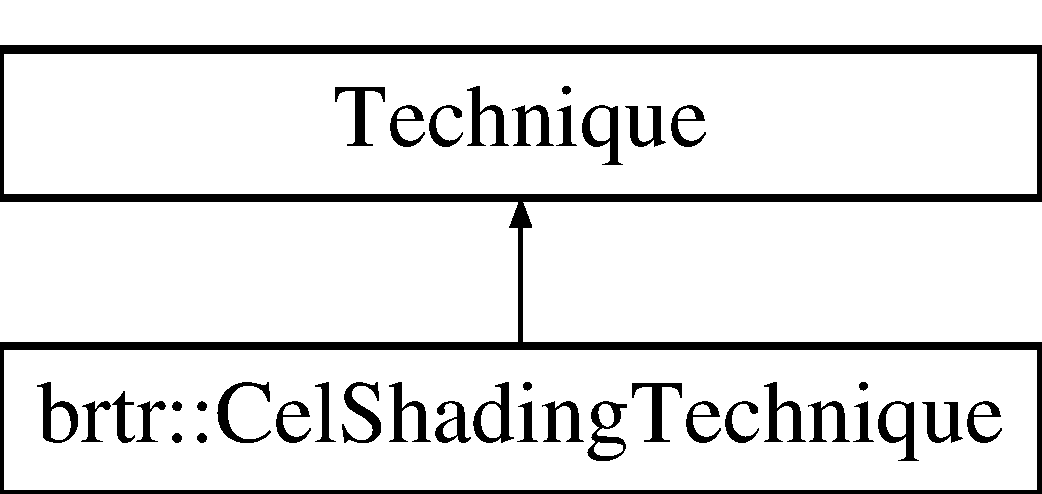
\includegraphics[height=2.000000cm]{classbrtr_1_1_cel_shading_technique}
\end{center}
\end{figure}
\subsection*{Public Member Functions}
\begin{DoxyCompactItemize}
\item 
\hyperlink{classbrtr_1_1_cel_shading_technique_a4c77c4f488907999068edd4d9b83aa4f}{Cel\+Shading\+Technique} (osg\+::\+Material $\ast$material, osg\+::\+Line\+Width $\ast$line\+Width, bool second\+Pass, std\+::string vert\+Source)
\end{DoxyCompactItemize}
\subsection*{Protected Member Functions}
\begin{DoxyCompactItemize}
\item 
void \hyperlink{classbrtr_1_1_cel_shading_technique_a7b44016e8ed4bc9c2c129b93de2f1f45}{define\+\_\+passes} ()
\end{DoxyCompactItemize}
\subsection*{Private Attributes}
\begin{DoxyCompactItemize}
\item 
osg\+::ref\+\_\+ptr$<$ osg\+::\+Material $>$ \hyperlink{classbrtr_1_1_cel_shading_technique_a266daa43a0effb4989755d61446dc14c}{\+\_\+material}
\item 
osg\+::ref\+\_\+ptr$<$ osg\+::\+Line\+Width $>$ \hyperlink{classbrtr_1_1_cel_shading_technique_a2b943ddfe4db5a92b959217a8321584f}{\+\_\+line\+Width}
\item 
std\+::string \hyperlink{classbrtr_1_1_cel_shading_technique_aca9e9164e2ccb2ce264786399713a8a6}{\+\_\+toon\+Tex}
\item 
bool \hyperlink{classbrtr_1_1_cel_shading_technique_a096109e6280cd43bb55762509a3e9f0c}{\+\_\+second\+Pass}
\item 
std\+::string \hyperlink{classbrtr_1_1_cel_shading_technique_a52a36916162a24d0ddd66d371fa04057}{\+\_\+vert\+Source}
\end{DoxyCompactItemize}


\subsection{Detailed Description}
The Technique for the cel-\/shading effect. 

\begin{DoxyAuthor}{Author}
Gleb Ostrowski 
\end{DoxyAuthor}
\begin{DoxyVersion}{Version}
1.\+0 
\end{DoxyVersion}
\begin{DoxyDate}{Date}
2014 
\end{DoxyDate}
\begin{DoxyCopyright}{Copyright}
G\+N\+U Public License. 
\end{DoxyCopyright}


Definition at line \hyperlink{_cel_shading_8cpp_source_l00022}{22} of file \hyperlink{_cel_shading_8cpp_source}{Cel\+Shading.\+cpp}.



\subsection{Constructor \& Destructor Documentation}
\hypertarget{classbrtr_1_1_cel_shading_technique_a4c77c4f488907999068edd4d9b83aa4f}{\index{brtr\+::\+Cel\+Shading\+Technique@{brtr\+::\+Cel\+Shading\+Technique}!Cel\+Shading\+Technique@{Cel\+Shading\+Technique}}
\index{Cel\+Shading\+Technique@{Cel\+Shading\+Technique}!brtr\+::\+Cel\+Shading\+Technique@{brtr\+::\+Cel\+Shading\+Technique}}
\subsubsection[{Cel\+Shading\+Technique}]{\setlength{\rightskip}{0pt plus 5cm}brtr\+::\+Cel\+Shading\+Technique\+::\+Cel\+Shading\+Technique (
\begin{DoxyParamCaption}
\item[{osg\+::\+Material $\ast$}]{material, }
\item[{osg\+::\+Line\+Width $\ast$}]{line\+Width, }
\item[{bool}]{second\+Pass, }
\item[{std\+::string}]{vert\+Source}
\end{DoxyParamCaption}
)\hspace{0.3cm}{\ttfamily [inline]}}}\label{classbrtr_1_1_cel_shading_technique_a4c77c4f488907999068edd4d9b83aa4f}


Definition at line \hyperlink{_cel_shading_8cpp_source_l00024}{24} of file \hyperlink{_cel_shading_8cpp_source}{Cel\+Shading.\+cpp}.



\subsection{Member Function Documentation}
\hypertarget{classbrtr_1_1_cel_shading_technique_a7b44016e8ed4bc9c2c129b93de2f1f45}{\index{brtr\+::\+Cel\+Shading\+Technique@{brtr\+::\+Cel\+Shading\+Technique}!define\+\_\+passes@{define\+\_\+passes}}
\index{define\+\_\+passes@{define\+\_\+passes}!brtr\+::\+Cel\+Shading\+Technique@{brtr\+::\+Cel\+Shading\+Technique}}
\subsubsection[{define\+\_\+passes}]{\setlength{\rightskip}{0pt plus 5cm}void brtr\+::\+Cel\+Shading\+Technique\+::define\+\_\+passes (
\begin{DoxyParamCaption}
{}
\end{DoxyParamCaption}
)\hspace{0.3cm}{\ttfamily [inline]}, {\ttfamily [protected]}}}\label{classbrtr_1_1_cel_shading_technique_a7b44016e8ed4bc9c2c129b93de2f1f45}


Definition at line \hyperlink{_cel_shading_8cpp_source_l00033}{33} of file \hyperlink{_cel_shading_8cpp_source}{Cel\+Shading.\+cpp}.



\subsection{Member Data Documentation}
\hypertarget{classbrtr_1_1_cel_shading_technique_a2b943ddfe4db5a92b959217a8321584f}{\index{brtr\+::\+Cel\+Shading\+Technique@{brtr\+::\+Cel\+Shading\+Technique}!\+\_\+line\+Width@{\+\_\+line\+Width}}
\index{\+\_\+line\+Width@{\+\_\+line\+Width}!brtr\+::\+Cel\+Shading\+Technique@{brtr\+::\+Cel\+Shading\+Technique}}
\subsubsection[{\+\_\+line\+Width}]{\setlength{\rightskip}{0pt plus 5cm}osg\+::ref\+\_\+ptr$<$osg\+::\+Line\+Width$>$ brtr\+::\+Cel\+Shading\+Technique\+::\+\_\+line\+Width\hspace{0.3cm}{\ttfamily [private]}}}\label{classbrtr_1_1_cel_shading_technique_a2b943ddfe4db5a92b959217a8321584f}


Definition at line \hyperlink{_cel_shading_8cpp_source_l00089}{89} of file \hyperlink{_cel_shading_8cpp_source}{Cel\+Shading.\+cpp}.

\hypertarget{classbrtr_1_1_cel_shading_technique_a266daa43a0effb4989755d61446dc14c}{\index{brtr\+::\+Cel\+Shading\+Technique@{brtr\+::\+Cel\+Shading\+Technique}!\+\_\+material@{\+\_\+material}}
\index{\+\_\+material@{\+\_\+material}!brtr\+::\+Cel\+Shading\+Technique@{brtr\+::\+Cel\+Shading\+Technique}}
\subsubsection[{\+\_\+material}]{\setlength{\rightskip}{0pt plus 5cm}osg\+::ref\+\_\+ptr$<$osg\+::\+Material$>$ brtr\+::\+Cel\+Shading\+Technique\+::\+\_\+material\hspace{0.3cm}{\ttfamily [private]}}}\label{classbrtr_1_1_cel_shading_technique_a266daa43a0effb4989755d61446dc14c}


Definition at line \hyperlink{_cel_shading_8cpp_source_l00088}{88} of file \hyperlink{_cel_shading_8cpp_source}{Cel\+Shading.\+cpp}.

\hypertarget{classbrtr_1_1_cel_shading_technique_a096109e6280cd43bb55762509a3e9f0c}{\index{brtr\+::\+Cel\+Shading\+Technique@{brtr\+::\+Cel\+Shading\+Technique}!\+\_\+second\+Pass@{\+\_\+second\+Pass}}
\index{\+\_\+second\+Pass@{\+\_\+second\+Pass}!brtr\+::\+Cel\+Shading\+Technique@{brtr\+::\+Cel\+Shading\+Technique}}
\subsubsection[{\+\_\+second\+Pass}]{\setlength{\rightskip}{0pt plus 5cm}bool brtr\+::\+Cel\+Shading\+Technique\+::\+\_\+second\+Pass\hspace{0.3cm}{\ttfamily [private]}}}\label{classbrtr_1_1_cel_shading_technique_a096109e6280cd43bb55762509a3e9f0c}


Definition at line \hyperlink{_cel_shading_8cpp_source_l00091}{91} of file \hyperlink{_cel_shading_8cpp_source}{Cel\+Shading.\+cpp}.

\hypertarget{classbrtr_1_1_cel_shading_technique_aca9e9164e2ccb2ce264786399713a8a6}{\index{brtr\+::\+Cel\+Shading\+Technique@{brtr\+::\+Cel\+Shading\+Technique}!\+\_\+toon\+Tex@{\+\_\+toon\+Tex}}
\index{\+\_\+toon\+Tex@{\+\_\+toon\+Tex}!brtr\+::\+Cel\+Shading\+Technique@{brtr\+::\+Cel\+Shading\+Technique}}
\subsubsection[{\+\_\+toon\+Tex}]{\setlength{\rightskip}{0pt plus 5cm}std\+::string brtr\+::\+Cel\+Shading\+Technique\+::\+\_\+toon\+Tex\hspace{0.3cm}{\ttfamily [private]}}}\label{classbrtr_1_1_cel_shading_technique_aca9e9164e2ccb2ce264786399713a8a6}


Definition at line \hyperlink{_cel_shading_8cpp_source_l00090}{90} of file \hyperlink{_cel_shading_8cpp_source}{Cel\+Shading.\+cpp}.

\hypertarget{classbrtr_1_1_cel_shading_technique_a52a36916162a24d0ddd66d371fa04057}{\index{brtr\+::\+Cel\+Shading\+Technique@{brtr\+::\+Cel\+Shading\+Technique}!\+\_\+vert\+Source@{\+\_\+vert\+Source}}
\index{\+\_\+vert\+Source@{\+\_\+vert\+Source}!brtr\+::\+Cel\+Shading\+Technique@{brtr\+::\+Cel\+Shading\+Technique}}
\subsubsection[{\+\_\+vert\+Source}]{\setlength{\rightskip}{0pt plus 5cm}std\+::string brtr\+::\+Cel\+Shading\+Technique\+::\+\_\+vert\+Source\hspace{0.3cm}{\ttfamily [private]}}}\label{classbrtr_1_1_cel_shading_technique_a52a36916162a24d0ddd66d371fa04057}


Definition at line \hyperlink{_cel_shading_8cpp_source_l00092}{92} of file \hyperlink{_cel_shading_8cpp_source}{Cel\+Shading.\+cpp}.



The documentation for this class was generated from the following file\+:\begin{DoxyCompactItemize}
\item 
Shader/\hyperlink{_cel_shading_8cpp}{Cel\+Shading.\+cpp}\end{DoxyCompactItemize}

\hypertarget{classbrtr_1_1_control_room}{\section{brtr\+:\+:Control\+Room Class Reference}
\label{classbrtr_1_1_control_room}\index{brtr\+::\+Control\+Room@{brtr\+::\+Control\+Room}}
}


Control Room Class, derived from Position\+Attitude\+Transform, set ups the whole room as its own children.  




{\ttfamily \#include $<$Control\+Room.\+h$>$}

Inheritance diagram for brtr\+:\+:Control\+Room\+:\begin{figure}[H]
\begin{center}
\leavevmode
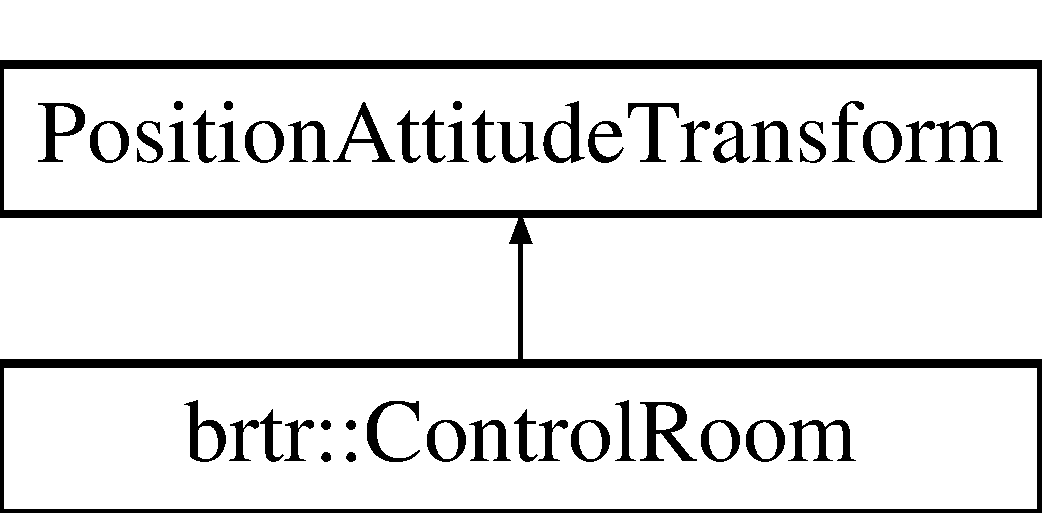
\includegraphics[height=2.000000cm]{classbrtr_1_1_control_room}
\end{center}
\end{figure}
\subsection*{Public Member Functions}
\begin{DoxyCompactItemize}
\item 
\hyperlink{classbrtr_1_1_control_room_afb36cd27e18234098fbecd22ac325319}{Control\+Room} (double room\+Size, int lod, \hyperlink{classbrtr_1_1_toon_tex_switcher_callback}{brtr\+::\+Toon\+Tex\+Switcher\+Callback} \&toon\+Callback, \hyperlink{classbrtr_1_1_program_switcher_callback}{brtr\+::\+Program\+Switcher\+Callback} \&program\+Callback)
\begin{DoxyCompactList}\small\item\em Constructor. \end{DoxyCompactList}\end{DoxyCompactItemize}
\subsection*{Protected Member Functions}
\begin{DoxyCompactItemize}
\item 
\hyperlink{classbrtr_1_1_control_room_a97b0eb95277b12a2267f8e7c777aeda2}{$\sim$\+Control\+Room} ()
\end{DoxyCompactItemize}
\subsection*{Private Member Functions}
\begin{DoxyCompactItemize}
\item 
osg\+::ref\+\_\+ptr$<$ osg\+::\+Group $>$ \hyperlink{classbrtr_1_1_control_room_a5dfafb496e18e8e4f6d792b144dd10b9}{create\+Room\+Surrounding} (double room\+Size, int lod)
\item 
osg\+::ref\+\_\+ptr$<$ osg\+::\+Group $>$ \hyperlink{classbrtr_1_1_control_room_a15055ae530b811b7046871c5c1ef3f4f}{create\+Chess\+Figures} (\hyperlink{classbrtr_1_1_toon_tex_switcher_callback}{brtr\+::\+Toon\+Tex\+Switcher\+Callback} \&toon\+Callback, \hyperlink{classbrtr_1_1_program_switcher_callback}{brtr\+::\+Program\+Switcher\+Callback} \&program\+Callback)
\item 
osg\+::ref\+\_\+ptr$<$ osg\+::\+Material $>$ \hyperlink{classbrtr_1_1_control_room_a1cb8b6799fcb85750e0d321a4fbed6f1}{create\+Material} (osg\+::\+Vec4 diffuse, osg\+::\+Vec4 ambient, osg\+::\+Vec4 specular=osg\+::\+Vec4(0.\+7, 0.\+7, 0.\+7, 1), double shininess=42.\+0)
\end{DoxyCompactItemize}


\subsection{Detailed Description}
Control Room Class, derived from Position\+Attitude\+Transform, set ups the whole room as its own children. 

sets always a light as light0, client should not use this light number any more the chess figures alongside with the provided interactioncallbacks are also set up \begin{DoxyAuthor}{Author}
Gleb Ostrowski 
\end{DoxyAuthor}
\begin{DoxyVersion}{Version}
1.\+0 
\end{DoxyVersion}
\begin{DoxyDate}{Date}
2014 
\end{DoxyDate}
\begin{DoxyCopyright}{Copyright}
G\+N\+U Public License. 
\end{DoxyCopyright}


Definition at line \hyperlink{_control_room_8h_source_l00018}{18} of file \hyperlink{_control_room_8h_source}{Control\+Room.\+h}.



\subsection{Constructor \& Destructor Documentation}
\hypertarget{classbrtr_1_1_control_room_afb36cd27e18234098fbecd22ac325319}{\index{brtr\+::\+Control\+Room@{brtr\+::\+Control\+Room}!Control\+Room@{Control\+Room}}
\index{Control\+Room@{Control\+Room}!brtr\+::\+Control\+Room@{brtr\+::\+Control\+Room}}
\subsubsection[{Control\+Room}]{\setlength{\rightskip}{0pt plus 5cm}brtr\+::\+Control\+Room\+::\+Control\+Room (
\begin{DoxyParamCaption}
\item[{double}]{room\+Size, }
\item[{int}]{lod, }
\item[{{\bf brtr\+::\+Toon\+Tex\+Switcher\+Callback} \&}]{toon\+Callback, }
\item[{{\bf brtr\+::\+Program\+Switcher\+Callback} \&}]{program\+Callback}
\end{DoxyParamCaption}
)}}\label{classbrtr_1_1_control_room_afb36cd27e18234098fbecd22ac325319}


Constructor. 


\begin{DoxyParams}{Parameters}
{\em room\+Size} & size of the room, height is roomsize/2 \\
\hline
{\em lod} & level of detail, the higher the more triangles are created \\
\hline
{\em toon\+Callback} & \hyperlink{classbrtr_1_1_toon_tex_switcher_callback}{Toon\+Tex\+Switcher\+Callback}, will be attached to first chess figure \\
\hline
{\em program\+Callback} & \hyperlink{classbrtr_1_1_program_switcher_callback}{Program\+Switcher\+Callback}, will be attached to third chess figure \\
\hline
\end{DoxyParams}


Definition at line \hyperlink{_control_room_8cpp_source_l00013}{13} of file \hyperlink{_control_room_8cpp_source}{Control\+Room.\+cpp}.

\hypertarget{classbrtr_1_1_control_room_a97b0eb95277b12a2267f8e7c777aeda2}{\index{brtr\+::\+Control\+Room@{brtr\+::\+Control\+Room}!````~Control\+Room@{$\sim$\+Control\+Room}}
\index{````~Control\+Room@{$\sim$\+Control\+Room}!brtr\+::\+Control\+Room@{brtr\+::\+Control\+Room}}
\subsubsection[{$\sim$\+Control\+Room}]{\setlength{\rightskip}{0pt plus 5cm}brtr\+::\+Control\+Room\+::$\sim$\+Control\+Room (
\begin{DoxyParamCaption}
{}
\end{DoxyParamCaption}
)\hspace{0.3cm}{\ttfamily [inline]}, {\ttfamily [protected]}}}\label{classbrtr_1_1_control_room_a97b0eb95277b12a2267f8e7c777aeda2}


Definition at line \hyperlink{_control_room_8h_source_l00031}{31} of file \hyperlink{_control_room_8h_source}{Control\+Room.\+h}.



\subsection{Member Function Documentation}
\hypertarget{classbrtr_1_1_control_room_a15055ae530b811b7046871c5c1ef3f4f}{\index{brtr\+::\+Control\+Room@{brtr\+::\+Control\+Room}!create\+Chess\+Figures@{create\+Chess\+Figures}}
\index{create\+Chess\+Figures@{create\+Chess\+Figures}!brtr\+::\+Control\+Room@{brtr\+::\+Control\+Room}}
\subsubsection[{create\+Chess\+Figures}]{\setlength{\rightskip}{0pt plus 5cm}ref\+\_\+ptr$<$ Group $>$ brtr\+::\+Control\+Room\+::create\+Chess\+Figures (
\begin{DoxyParamCaption}
\item[{{\bf brtr\+::\+Toon\+Tex\+Switcher\+Callback} \&}]{toon\+Callback, }
\item[{{\bf brtr\+::\+Program\+Switcher\+Callback} \&}]{program\+Callback}
\end{DoxyParamCaption}
)\hspace{0.3cm}{\ttfamily [private]}}}\label{classbrtr_1_1_control_room_a15055ae530b811b7046871c5c1ef3f4f}


Definition at line \hyperlink{_control_room_8cpp_source_l00100}{100} of file \hyperlink{_control_room_8cpp_source}{Control\+Room.\+cpp}.

\hypertarget{classbrtr_1_1_control_room_a1cb8b6799fcb85750e0d321a4fbed6f1}{\index{brtr\+::\+Control\+Room@{brtr\+::\+Control\+Room}!create\+Material@{create\+Material}}
\index{create\+Material@{create\+Material}!brtr\+::\+Control\+Room@{brtr\+::\+Control\+Room}}
\subsubsection[{create\+Material}]{\setlength{\rightskip}{0pt plus 5cm}ref\+\_\+ptr$<$ Material $>$ brtr\+::\+Control\+Room\+::create\+Material (
\begin{DoxyParamCaption}
\item[{osg\+::\+Vec4}]{diffuse, }
\item[{osg\+::\+Vec4}]{ambient, }
\item[{osg\+::\+Vec4}]{specular = {\ttfamily osg\+:\+:Vec4(0.7,0.7,0.7,1)}, }
\item[{double}]{shininess = {\ttfamily 42.0}}
\end{DoxyParamCaption}
)\hspace{0.3cm}{\ttfamily [private]}}}\label{classbrtr_1_1_control_room_a1cb8b6799fcb85750e0d321a4fbed6f1}


Definition at line \hyperlink{_control_room_8cpp_source_l00145}{145} of file \hyperlink{_control_room_8cpp_source}{Control\+Room.\+cpp}.

\hypertarget{classbrtr_1_1_control_room_a5dfafb496e18e8e4f6d792b144dd10b9}{\index{brtr\+::\+Control\+Room@{brtr\+::\+Control\+Room}!create\+Room\+Surrounding@{create\+Room\+Surrounding}}
\index{create\+Room\+Surrounding@{create\+Room\+Surrounding}!brtr\+::\+Control\+Room@{brtr\+::\+Control\+Room}}
\subsubsection[{create\+Room\+Surrounding}]{\setlength{\rightskip}{0pt plus 5cm}ref\+\_\+ptr$<$ Group $>$ brtr\+::\+Control\+Room\+::create\+Room\+Surrounding (
\begin{DoxyParamCaption}
\item[{double}]{room\+Size, }
\item[{int}]{lod}
\end{DoxyParamCaption}
)\hspace{0.3cm}{\ttfamily [private]}}}\label{classbrtr_1_1_control_room_a5dfafb496e18e8e4f6d792b144dd10b9}


Definition at line \hyperlink{_control_room_8cpp_source_l00026}{26} of file \hyperlink{_control_room_8cpp_source}{Control\+Room.\+cpp}.



The documentation for this class was generated from the following files\+:\begin{DoxyCompactItemize}
\item 
header/\hyperlink{_control_room_8h}{Control\+Room.\+h}\item 
Objects/\hyperlink{_control_room_8cpp}{Control\+Room.\+cpp}\end{DoxyCompactItemize}

\hypertarget{classbrtr_1_1_drunken_interaction_callback}{\section{brtr\+:\+:Drunken\+Interaction\+Callback Class Reference}
\label{classbrtr_1_1_drunken_interaction_callback}\index{brtr\+::\+Drunken\+Interaction\+Callback@{brtr\+::\+Drunken\+Interaction\+Callback}}
}


Callback for the drunk effect.  




{\ttfamily \#include $<$Drunken\+Interaction\+Callback.\+h$>$}

Inheritance diagram for brtr\+:\+:Drunken\+Interaction\+Callback\+:\begin{figure}[H]
\begin{center}
\leavevmode
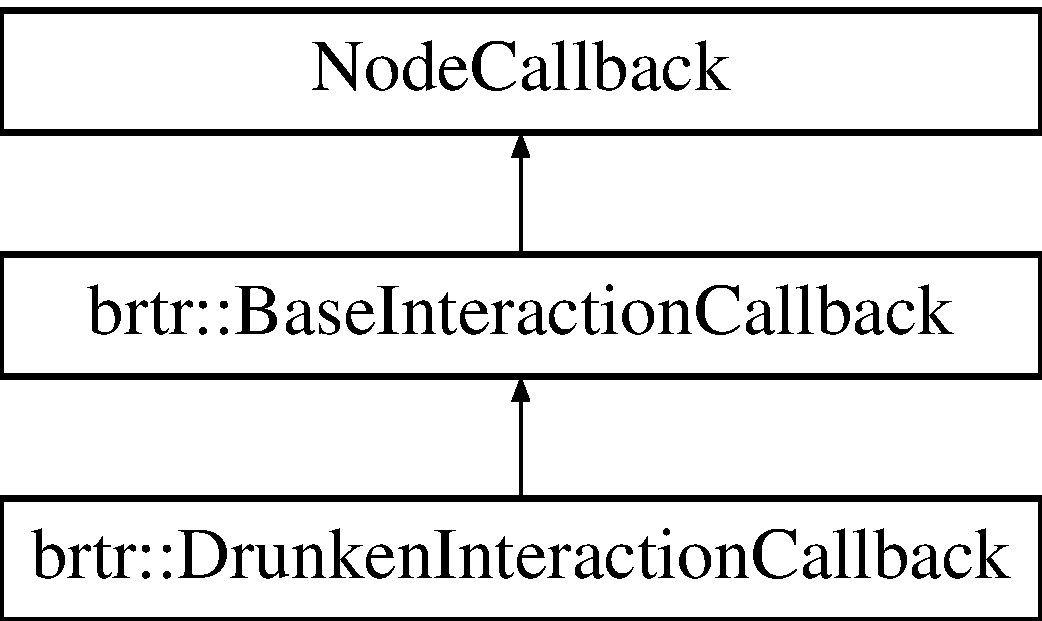
\includegraphics[height=3.000000cm]{classbrtr_1_1_drunken_interaction_callback}
\end{center}
\end{figure}
\subsection*{Public Member Functions}
\begin{DoxyCompactItemize}
\item 
\hyperlink{classbrtr_1_1_drunken_interaction_callback_aa252ac5f3bc393ecb75784b98e17b5a5}{Drunken\+Interaction\+Callback} (osg\+::\+Node $\ast$camera, osg\+::\+Camera $\ast$hud\+Cam, osg\+::\+Switch $\ast$geometry\+Switch, int width, int height)
\begin{DoxyCompactList}\small\item\em Constructor. \end{DoxyCompactList}\item 
virtual void \hyperlink{classbrtr_1_1_drunken_interaction_callback_a71b86fc410bf2965ca998eff1350cfaf}{set\+Text} ()
\begin{DoxyCompactList}\small\item\em sets the text on screen. Subclasses must override to set its own (info)text \end{DoxyCompactList}\end{DoxyCompactItemize}
\subsection*{Protected Member Functions}
\begin{DoxyCompactItemize}
\item 
virtual void \hyperlink{classbrtr_1_1_drunken_interaction_callback_a86e4062f00a33768f752c1c5fa50c291}{interact} (osg\+::\+Node $\ast$, osg\+::\+Node\+Visitor $\ast$)
\begin{DoxyCompactList}\small\item\em Drunk effect is simulated by changing the F\+O\+V of the projection matrix. \end{DoxyCompactList}\end{DoxyCompactItemize}
\subsection*{Private Attributes}
\begin{DoxyCompactItemize}
\item 
int \hyperlink{classbrtr_1_1_drunken_interaction_callback_ab1a42a563e42cfd1d480741b30e22245}{\+\_\+start\+Time}
\item 
osg\+::ref\+\_\+ptr$<$ osg\+::\+Switch $>$ \hyperlink{classbrtr_1_1_drunken_interaction_callback_a0aa1983e0fc1cb720badb80464a8e391}{\+\_\+geometry\+Switch}
\item 
osg\+::ref\+\_\+ptr\\*
$<$ osg\+Animation\+::\+Linear\+Motion $>$ \hyperlink{classbrtr_1_1_drunken_interaction_callback_adaa3e659a9f6516a5b59a43813506a11}{\+\_\+motion}
\item 
bool \hyperlink{classbrtr_1_1_drunken_interaction_callback_a4be32ea919b41bd46acc34904fb5c7b7}{\+\_\+backwards}
\end{DoxyCompactItemize}
\subsection*{Additional Inherited Members}


\subsection{Detailed Description}
Callback for the drunk effect. 

\begin{DoxyAuthor}{Author}
Gleb Ostrowski 
\end{DoxyAuthor}
\begin{DoxyVersion}{Version}
1.\+0 
\end{DoxyVersion}
\begin{DoxyDate}{Date}
2014 
\end{DoxyDate}
\begin{DoxyCopyright}{Copyright}
G\+N\+U Public License. 
\end{DoxyCopyright}


Definition at line \hyperlink{_drunken_interaction_callback_8h_source_l00015}{15} of file \hyperlink{_drunken_interaction_callback_8h_source}{Drunken\+Interaction\+Callback.\+h}.



\subsection{Constructor \& Destructor Documentation}
\hypertarget{classbrtr_1_1_drunken_interaction_callback_aa252ac5f3bc393ecb75784b98e17b5a5}{\index{brtr\+::\+Drunken\+Interaction\+Callback@{brtr\+::\+Drunken\+Interaction\+Callback}!Drunken\+Interaction\+Callback@{Drunken\+Interaction\+Callback}}
\index{Drunken\+Interaction\+Callback@{Drunken\+Interaction\+Callback}!brtr\+::\+Drunken\+Interaction\+Callback@{brtr\+::\+Drunken\+Interaction\+Callback}}
\subsubsection[{Drunken\+Interaction\+Callback}]{\setlength{\rightskip}{0pt plus 5cm}brtr\+::\+Drunken\+Interaction\+Callback\+::\+Drunken\+Interaction\+Callback (
\begin{DoxyParamCaption}
\item[{osg\+::\+Node $\ast$}]{camera, }
\item[{osg\+::\+Camera $\ast$}]{hud\+Cam, }
\item[{osg\+::\+Switch $\ast$}]{geometry\+Switch, }
\item[{int}]{width, }
\item[{int}]{height}
\end{DoxyParamCaption}
)}}\label{classbrtr_1_1_drunken_interaction_callback_aa252ac5f3bc393ecb75784b98e17b5a5}


Constructor. 


\begin{DoxyParams}{Parameters}
{\em camera} & the camera, whichs projection matrix will be manipulated \\
\hline
{\em hud\+Cam} & \\
\hline
{\em geometry\+Switch} & switch containing the bottle, for removing it after the interaction \\
\hline
{\em width} & screenwidth \\
\hline
{\em height} & screenheight \\
\hline
\end{DoxyParams}


Definition at line \hyperlink{_drunken_interaction_callback_8cpp_source_l00005}{5} of file \hyperlink{_drunken_interaction_callback_8cpp_source}{Drunken\+Interaction\+Callback.\+cpp}.



\subsection{Member Function Documentation}
\hypertarget{classbrtr_1_1_drunken_interaction_callback_a86e4062f00a33768f752c1c5fa50c291}{\index{brtr\+::\+Drunken\+Interaction\+Callback@{brtr\+::\+Drunken\+Interaction\+Callback}!interact@{interact}}
\index{interact@{interact}!brtr\+::\+Drunken\+Interaction\+Callback@{brtr\+::\+Drunken\+Interaction\+Callback}}
\subsubsection[{interact}]{\setlength{\rightskip}{0pt plus 5cm}void brtr\+::\+Drunken\+Interaction\+Callback\+::interact (
\begin{DoxyParamCaption}
\item[{osg\+::\+Node $\ast$}]{node, }
\item[{osg\+::\+Node\+Visitor $\ast$}]{nv}
\end{DoxyParamCaption}
)\hspace{0.3cm}{\ttfamily [protected]}, {\ttfamily [virtual]}}}\label{classbrtr_1_1_drunken_interaction_callback_a86e4062f00a33768f752c1c5fa50c291}


Drunk effect is simulated by changing the F\+O\+V of the projection matrix. 


\begin{DoxyParams}{Parameters}
{\em not} & needed \\
\hline
{\em not} & needed \\
\hline
\end{DoxyParams}


Implements \hyperlink{classbrtr_1_1_base_interaction_callback_a3ed50c9c1725f932e0b78c90ba24e1ed}{brtr\+::\+Base\+Interaction\+Callback}.



Definition at line \hyperlink{_drunken_interaction_callback_8cpp_source_l00013}{13} of file \hyperlink{_drunken_interaction_callback_8cpp_source}{Drunken\+Interaction\+Callback.\+cpp}.

\hypertarget{classbrtr_1_1_drunken_interaction_callback_a71b86fc410bf2965ca998eff1350cfaf}{\index{brtr\+::\+Drunken\+Interaction\+Callback@{brtr\+::\+Drunken\+Interaction\+Callback}!set\+Text@{set\+Text}}
\index{set\+Text@{set\+Text}!brtr\+::\+Drunken\+Interaction\+Callback@{brtr\+::\+Drunken\+Interaction\+Callback}}
\subsubsection[{set\+Text}]{\setlength{\rightskip}{0pt plus 5cm}void brtr\+::\+Drunken\+Interaction\+Callback\+::set\+Text (
\begin{DoxyParamCaption}
{}
\end{DoxyParamCaption}
)\hspace{0.3cm}{\ttfamily [virtual]}}}\label{classbrtr_1_1_drunken_interaction_callback_a71b86fc410bf2965ca998eff1350cfaf}


sets the text on screen. Subclasses must override to set its own (info)text 



Implements \hyperlink{classbrtr_1_1_base_interaction_callback_a0fe57e329f044e21d49041c861435ad8}{brtr\+::\+Base\+Interaction\+Callback}.



Definition at line \hyperlink{_drunken_interaction_callback_8cpp_source_l00044}{44} of file \hyperlink{_drunken_interaction_callback_8cpp_source}{Drunken\+Interaction\+Callback.\+cpp}.



\subsection{Member Data Documentation}
\hypertarget{classbrtr_1_1_drunken_interaction_callback_a4be32ea919b41bd46acc34904fb5c7b7}{\index{brtr\+::\+Drunken\+Interaction\+Callback@{brtr\+::\+Drunken\+Interaction\+Callback}!\+\_\+backwards@{\+\_\+backwards}}
\index{\+\_\+backwards@{\+\_\+backwards}!brtr\+::\+Drunken\+Interaction\+Callback@{brtr\+::\+Drunken\+Interaction\+Callback}}
\subsubsection[{\+\_\+backwards}]{\setlength{\rightskip}{0pt plus 5cm}bool brtr\+::\+Drunken\+Interaction\+Callback\+::\+\_\+backwards\hspace{0.3cm}{\ttfamily [private]}}}\label{classbrtr_1_1_drunken_interaction_callback_a4be32ea919b41bd46acc34904fb5c7b7}


Definition at line \hyperlink{_drunken_interaction_callback_8h_source_l00042}{42} of file \hyperlink{_drunken_interaction_callback_8h_source}{Drunken\+Interaction\+Callback.\+h}.

\hypertarget{classbrtr_1_1_drunken_interaction_callback_a0aa1983e0fc1cb720badb80464a8e391}{\index{brtr\+::\+Drunken\+Interaction\+Callback@{brtr\+::\+Drunken\+Interaction\+Callback}!\+\_\+geometry\+Switch@{\+\_\+geometry\+Switch}}
\index{\+\_\+geometry\+Switch@{\+\_\+geometry\+Switch}!brtr\+::\+Drunken\+Interaction\+Callback@{brtr\+::\+Drunken\+Interaction\+Callback}}
\subsubsection[{\+\_\+geometry\+Switch}]{\setlength{\rightskip}{0pt plus 5cm}osg\+::ref\+\_\+ptr$<$osg\+::\+Switch$>$ brtr\+::\+Drunken\+Interaction\+Callback\+::\+\_\+geometry\+Switch\hspace{0.3cm}{\ttfamily [private]}}}\label{classbrtr_1_1_drunken_interaction_callback_a0aa1983e0fc1cb720badb80464a8e391}


Definition at line \hyperlink{_drunken_interaction_callback_8h_source_l00040}{40} of file \hyperlink{_drunken_interaction_callback_8h_source}{Drunken\+Interaction\+Callback.\+h}.

\hypertarget{classbrtr_1_1_drunken_interaction_callback_adaa3e659a9f6516a5b59a43813506a11}{\index{brtr\+::\+Drunken\+Interaction\+Callback@{brtr\+::\+Drunken\+Interaction\+Callback}!\+\_\+motion@{\+\_\+motion}}
\index{\+\_\+motion@{\+\_\+motion}!brtr\+::\+Drunken\+Interaction\+Callback@{brtr\+::\+Drunken\+Interaction\+Callback}}
\subsubsection[{\+\_\+motion}]{\setlength{\rightskip}{0pt plus 5cm}osg\+::ref\+\_\+ptr$<$osg\+Animation\+::\+Linear\+Motion$>$ brtr\+::\+Drunken\+Interaction\+Callback\+::\+\_\+motion\hspace{0.3cm}{\ttfamily [private]}}}\label{classbrtr_1_1_drunken_interaction_callback_adaa3e659a9f6516a5b59a43813506a11}


Definition at line \hyperlink{_drunken_interaction_callback_8h_source_l00041}{41} of file \hyperlink{_drunken_interaction_callback_8h_source}{Drunken\+Interaction\+Callback.\+h}.

\hypertarget{classbrtr_1_1_drunken_interaction_callback_ab1a42a563e42cfd1d480741b30e22245}{\index{brtr\+::\+Drunken\+Interaction\+Callback@{brtr\+::\+Drunken\+Interaction\+Callback}!\+\_\+start\+Time@{\+\_\+start\+Time}}
\index{\+\_\+start\+Time@{\+\_\+start\+Time}!brtr\+::\+Drunken\+Interaction\+Callback@{brtr\+::\+Drunken\+Interaction\+Callback}}
\subsubsection[{\+\_\+start\+Time}]{\setlength{\rightskip}{0pt plus 5cm}int brtr\+::\+Drunken\+Interaction\+Callback\+::\+\_\+start\+Time\hspace{0.3cm}{\ttfamily [private]}}}\label{classbrtr_1_1_drunken_interaction_callback_ab1a42a563e42cfd1d480741b30e22245}


Definition at line \hyperlink{_drunken_interaction_callback_8h_source_l00039}{39} of file \hyperlink{_drunken_interaction_callback_8h_source}{Drunken\+Interaction\+Callback.\+h}.



The documentation for this class was generated from the following files\+:\begin{DoxyCompactItemize}
\item 
header/\hyperlink{_drunken_interaction_callback_8h}{Drunken\+Interaction\+Callback.\+h}\item 
Callbacks/\hyperlink{_drunken_interaction_callback_8cpp}{Drunken\+Interaction\+Callback.\+cpp}\end{DoxyCompactItemize}

\hypertarget{classbrtr_1_1_f_p_s_camera_manipulator}{\section{brtr\+:\+:F\+P\+S\+Camera\+Manipulator Class Reference}
\label{classbrtr_1_1_f_p_s_camera_manipulator}\index{brtr\+::\+F\+P\+S\+Camera\+Manipulator@{brtr\+::\+F\+P\+S\+Camera\+Manipulator}}
}


A F\+P\+S style Camera\+Manipulator with ground clamping and intersection.  




{\ttfamily \#include $<$F\+P\+S\+Camera\+Manipulator.\+h$>$}

Inheritance diagram for brtr\+:\+:F\+P\+S\+Camera\+Manipulator\+:\begin{figure}[H]
\begin{center}
\leavevmode
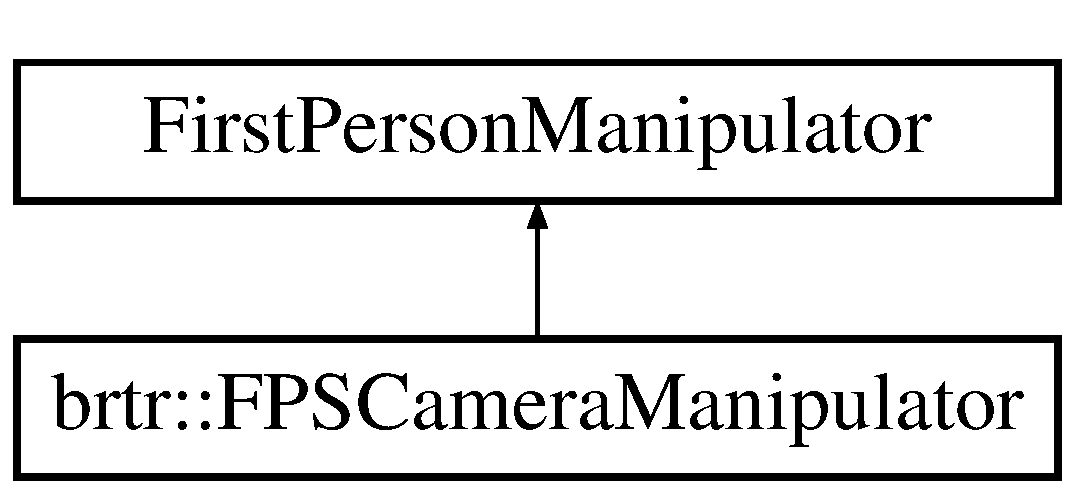
\includegraphics[height=2.000000cm]{classbrtr_1_1_f_p_s_camera_manipulator}
\end{center}
\end{figure}
\subsection*{Public Member Functions}
\begin{DoxyCompactItemize}
\item 
\hyperlink{classbrtr_1_1_f_p_s_camera_manipulator_aaf8bf3f6db925ba6c7d4a3157edcede3}{F\+P\+S\+Camera\+Manipulator} (double movement\+Speed, double z\+Height, osg\+::\+Node $\ast$root, bool flight\+Mode=false)
\begin{DoxyCompactList}\small\item\em Constructor. \end{DoxyCompactList}\item 
double \hyperlink{classbrtr_1_1_f_p_s_camera_manipulator_a3c576fd94a834b4712c30280ebc38763}{get\+Movement\+Speed} () const 
\item 
\hyperlink{classbrtr_1_1_f_p_s_camera_manipulator}{F\+P\+S\+Camera\+Manipulator} \& \hyperlink{classbrtr_1_1_f_p_s_camera_manipulator_a778a95c8fa5c22d9c5e3bdde5e8c6591}{set\+Movement\+Speed} (double val)
\item 
double \hyperlink{classbrtr_1_1_f_p_s_camera_manipulator_ad564a29e30a95676a64b06160ba9e6ea}{get\+Z\+Height} () const 
\item 
\hyperlink{classbrtr_1_1_f_p_s_camera_manipulator}{F\+P\+S\+Camera\+Manipulator} \& \hyperlink{classbrtr_1_1_f_p_s_camera_manipulator_a71f558339f33edf1fa8cf81faf5914aa}{set\+Z\+Height} (double val)
\item 
double \hyperlink{classbrtr_1_1_f_p_s_camera_manipulator_a409f00bd591ea3f847319794d4e0f15d}{get\+Jump\+Height} () const 
\item 
\hyperlink{classbrtr_1_1_f_p_s_camera_manipulator}{F\+P\+S\+Camera\+Manipulator} \& \hyperlink{classbrtr_1_1_f_p_s_camera_manipulator_a8bf29fb4cf8f0d8842b7b0ac798e23cb}{set\+Jump\+Height} (double val)
\end{DoxyCompactItemize}
\subsection*{Protected Member Functions}
\begin{DoxyCompactItemize}
\item 
\hyperlink{classbrtr_1_1_f_p_s_camera_manipulator_a9f18b06a1f730f39da8fb7bdf960c3a9}{$\sim$\+F\+P\+S\+Camera\+Manipulator} ()
\item 
virtual bool \hyperlink{classbrtr_1_1_f_p_s_camera_manipulator_a2f6319fa6eb148e2f5b59688b38891ae}{handle\+Mouse\+Move} (const osg\+G\+A\+::\+G\+U\+I\+Event\+Adapter \&ea, osg\+G\+A\+::\+G\+U\+I\+Action\+Adapter \&us)
\begin{DoxyCompactList}\small\item\em Handles the movement of the mouse. \end{DoxyCompactList}\item 
virtual bool \hyperlink{classbrtr_1_1_f_p_s_camera_manipulator_abad7544ac96384f79b2fa0d5d91606f6}{handle\+Frame} (const osg\+G\+A\+::\+G\+U\+I\+Event\+Adapter \&ea, osg\+G\+A\+::\+G\+U\+I\+Action\+Adapter \&us)
\begin{DoxyCompactList}\small\item\em Handles, what happens every frame. \end{DoxyCompactList}\item 
virtual bool \hyperlink{classbrtr_1_1_f_p_s_camera_manipulator_ad12557e5ce643476c8850c91a59e4956}{handle\+Key\+Down} (const osg\+G\+A\+::\+G\+U\+I\+Event\+Adapter \&ea, osg\+G\+A\+::\+G\+U\+I\+Action\+Adapter \&us)
\begin{DoxyCompactList}\small\item\em Handle key down presses. For supported keys see the class desc. \end{DoxyCompactList}\item 
virtual bool \hyperlink{classbrtr_1_1_f_p_s_camera_manipulator_a165a843388846d16426adcf0cd870b5e}{handle\+Key\+Up} (const osg\+G\+A\+::\+G\+U\+I\+Event\+Adapter \&ea, osg\+G\+A\+::\+G\+U\+I\+Action\+Adapter \&us)
\begin{DoxyCompactList}\small\item\em Handle key up presses. For supported keys see the class desc. \end{DoxyCompactList}\item 
virtual bool \hyperlink{classbrtr_1_1_f_p_s_camera_manipulator_a5c9aa59e32263262b24595ecf57dace6}{perform\+Movement} ()
\begin{DoxyCompactList}\small\item\em Mouse\+Look is implemented in this method. \end{DoxyCompactList}\item 
virtual bool \hyperlink{classbrtr_1_1_f_p_s_camera_manipulator_acbda7c2bbd00f5b143723bd7a85f9e9d}{perform\+Movement\+Left\+Mouse\+Button} (const double event\+Time\+Delta, const double dx, const double dy)
\item 
virtual bool \hyperlink{classbrtr_1_1_f_p_s_camera_manipulator_a02b5f77aca53a0974b81d0dfadd811cd}{handle\+Mouse\+Wheel} (const osg\+G\+A\+::\+G\+U\+I\+Event\+Adapter \&ea, osg\+G\+A\+::\+G\+U\+I\+Action\+Adapter \&us)
\end{DoxyCompactItemize}
\subsection*{Private Member Functions}
\begin{DoxyCompactItemize}
\item 
bool \hyperlink{classbrtr_1_1_f_p_s_camera_manipulator_aac9cc9e147b61f0afee6d02a98584271}{perform\+Eye\+Movement} ()
\begin{DoxyCompactList}\small\item\em moves the camera\+Eye, checking various conditions \end{DoxyCompactList}\item 
bool \hyperlink{classbrtr_1_1_f_p_s_camera_manipulator_af6bc3644bd39ad6f8fed053dc97aeb0e}{intersect} (const osg\+::\+Vec3d start, const osg\+::\+Vec3d end, double \&distance)
\begin{DoxyCompactList}\small\item\em Finds the distance between start and end intersection, if there is any. \end{DoxyCompactList}\item 
bool \hyperlink{classbrtr_1_1_f_p_s_camera_manipulator_a8df110e35ccce81c7fac9d7719a60797}{ground\+Intersection} (osg\+::\+Vec3d \&new\+Eye)
\begin{DoxyCompactList}\small\item\em checks, whether the new\+Eye is still clamped to ground \end{DoxyCompactList}\end{DoxyCompactItemize}
\subsection*{Private Attributes}
\begin{DoxyCompactItemize}
\item 
osg\+::ref\+\_\+ptr\\*
$<$ osg\+::\+Position\+Attitude\+Transform $>$ \hyperlink{classbrtr_1_1_f_p_s_camera_manipulator_ad1e35379f9ec8d6a6fc46441b6d8ae0d}{\+\_\+body}
\item 
bool \hyperlink{classbrtr_1_1_f_p_s_camera_manipulator_a1fd26cbf63923d5999eb10009e599e64}{\+\_\+flight\+Mode}
\item 
bool \hyperlink{classbrtr_1_1_f_p_s_camera_manipulator_abc82a762cc644b34c4778ccd89c61f2a}{\+\_\+forward\+Movement}
\item 
bool \hyperlink{classbrtr_1_1_f_p_s_camera_manipulator_a1fadc5283652e5bced25ed8c206b6e60}{\+\_\+backward\+Movement}
\item 
bool \hyperlink{classbrtr_1_1_f_p_s_camera_manipulator_aebebc4754eb8e12d0d9eb3a304196473}{\+\_\+left\+Movement}
\item 
bool \hyperlink{classbrtr_1_1_f_p_s_camera_manipulator_a681ef6c8b6cb2250d5f6dee155e3d357}{\+\_\+right\+Movement}
\item 
bool \hyperlink{classbrtr_1_1_f_p_s_camera_manipulator_ab63f237cc4d2a05b65f8168d55ad788e}{\+\_\+up\+Movement}
\item 
bool \hyperlink{classbrtr_1_1_f_p_s_camera_manipulator_ad4e208525965da8d36fb243d5fe1903e}{\+\_\+down\+Movement}
\item 
bool \hyperlink{classbrtr_1_1_f_p_s_camera_manipulator_aa97b8839047c137842b05410eadb828e}{\+\_\+attach\+Body}
\item 
bool \hyperlink{classbrtr_1_1_f_p_s_camera_manipulator_a189d9907cc38cf12b79a7ffc4e815843}{\+\_\+shift}
\item 
bool \hyperlink{classbrtr_1_1_f_p_s_camera_manipulator_a9eaba9401245f5f1912ff91a751fed20}{\+\_\+ctrl}
\item 
bool \hyperlink{classbrtr_1_1_f_p_s_camera_manipulator_a704712caf668c5989e5a9231f9d71022}{\+\_\+jumping\+Up}
\item 
bool \hyperlink{classbrtr_1_1_f_p_s_camera_manipulator_a2041c39f1ba8c5450f7c5472701c9cd8}{\+\_\+jumping\+Down}
\item 
bool \hyperlink{classbrtr_1_1_f_p_s_camera_manipulator_ab9c1187fd128b8de757af5d0ecb65b28}{\+\_\+crouch}
\item 
double \hyperlink{classbrtr_1_1_f_p_s_camera_manipulator_afff7ee29460f89132b682aa31ed346a6}{\+\_\+max\+Fall\+Height}
\item 
double \hyperlink{classbrtr_1_1_f_p_s_camera_manipulator_abbc7acdd7a7e643d6e25bf453ac9f1dd}{\+\_\+movement\+Speed}
\item 
double \hyperlink{classbrtr_1_1_f_p_s_camera_manipulator_aef10149826f951be3dc1b3d7b7f6b334}{\+\_\+z\+Height}
\item 
double \hyperlink{classbrtr_1_1_f_p_s_camera_manipulator_a6e05c375307130a1e45d69a18760f439}{\+\_\+savedz\+Height}
\item 
double \hyperlink{classbrtr_1_1_f_p_s_camera_manipulator_a00283025e62ab200588340a8a11bbc20}{\+\_\+intensity}
\item 
double \hyperlink{classbrtr_1_1_f_p_s_camera_manipulator_a3638230e6c3c59072caab0dcef0b5371}{\+\_\+frame\+Factor}
\item 
double \hyperlink{classbrtr_1_1_f_p_s_camera_manipulator_af1c207c0b72b4124db14bd1983deeb62}{\+\_\+body\+Length}
\item 
double \hyperlink{classbrtr_1_1_f_p_s_camera_manipulator_a53d486248c35c9e70436ebf0dea14b64}{\+\_\+jump\+Height}
\item 
double \hyperlink{classbrtr_1_1_f_p_s_camera_manipulator_a08dab67599aa8d6d7bc7409f33773da8}{\+\_\+savedz\+Height\+Crouch}
\end{DoxyCompactItemize}


\subsection{Detailed Description}
A F\+P\+S style Camera\+Manipulator with ground clamping and intersection. 

\begin{DoxyParagraph}{Controls\+: }

\begin{DoxyPre}
                   W       = Move forward.
                 A S D     = (A)=Move Left, (S)=Move backward, (D)=Move Right.
                   F       = Toggle FlightMode on/off
                 Q / E     = Up/Down (in FlightMode)
                   G       = Attach/Detach Body
                   X       = Crouch
                 SPACE     = Jump (if not flying)
                 SHIFT     = Sprint
                 CTRL      = Walk
             \end{DoxyPre}
 Inspiration for Intersection and Clamping Testing\+: ~\newline
 Official O\+S\+G Source (mostly Drive\+Manipulator)~\newline
 Game\+Manipulator and Pod by Viggo L�vli, \href{http://markmail.org/message/e6magjobl7fywbe6}{\tt http\+://markmail.\+org/message/e6magjobl7fywbe6} , visited 26/05/2014~\newline
 For Nodes, which should be passable regardless of Flight\+Mode (e.\+g. Fake\+Walls) one must set the ~\newline
 Node\+Mask to $\sim$brtr\hyperlink{namespacebrtr_af79a815819e2ef65ea9cd43dc9d43679}{collision\+Mask} ~\newline
 Body Code not used anymore (we did not like it). Not deleted, because it works. 
\end{DoxyParagraph}
\begin{DoxyAuthor}{Author}
Gleb Ostrowski 
\end{DoxyAuthor}
\begin{DoxyVersion}{Version}
1.\+0 
\end{DoxyVersion}
\begin{DoxyDate}{Date}
06/2014 
\end{DoxyDate}
\begin{DoxyPrecond}{Precondition}
Need to be attached to a viewer, so, create a viewer first 
\end{DoxyPrecond}
\begin{DoxyRefDesc}{Bug}
\item[\hyperlink{bug__bug000001}{Bug}]Jumping forward if there is no ground is not working~\newline
\end{DoxyRefDesc}


\begin{DoxyCopyright}{Copyright}
G\+N\+U Public License. 
\end{DoxyCopyright}


Definition at line \hyperlink{_f_p_s_camera_manipulator_8h_source_l00033}{33} of file \hyperlink{_f_p_s_camera_manipulator_8h_source}{F\+P\+S\+Camera\+Manipulator.\+h}.



\subsection{Constructor \& Destructor Documentation}
\hypertarget{classbrtr_1_1_f_p_s_camera_manipulator_aaf8bf3f6db925ba6c7d4a3157edcede3}{\index{brtr\+::\+F\+P\+S\+Camera\+Manipulator@{brtr\+::\+F\+P\+S\+Camera\+Manipulator}!F\+P\+S\+Camera\+Manipulator@{F\+P\+S\+Camera\+Manipulator}}
\index{F\+P\+S\+Camera\+Manipulator@{F\+P\+S\+Camera\+Manipulator}!brtr\+::\+F\+P\+S\+Camera\+Manipulator@{brtr\+::\+F\+P\+S\+Camera\+Manipulator}}
\subsubsection[{F\+P\+S\+Camera\+Manipulator}]{\setlength{\rightskip}{0pt plus 5cm}brtr\+::\+F\+P\+S\+Camera\+Manipulator\+::\+F\+P\+S\+Camera\+Manipulator (
\begin{DoxyParamCaption}
\item[{double}]{movement\+Speed, }
\item[{double}]{z\+Height, }
\item[{osg\+::\+Node $\ast$}]{root, }
\item[{bool}]{flight\+Mode = {\ttfamily false}}
\end{DoxyParamCaption}
)}}\label{classbrtr_1_1_f_p_s_camera_manipulator_aaf8bf3f6db925ba6c7d4a3157edcede3}


Constructor. 


\begin{DoxyParams}{Parameters}
{\em movement\+Speed} & the player \char`\"{}movement\char`\"{} speed \\
\hline
{\em z\+Height} & the camera height \\
\hline
{\em root} & root node for attaching the body to, not used anymore \\
\hline
{\em flight\+Mode} & flightmoe true or false in the beginning \\
\hline
\end{DoxyParams}


Definition at line \hyperlink{_f_p_s_camera_manipulator_8cpp_source_l00012}{12} of file \hyperlink{_f_p_s_camera_manipulator_8cpp_source}{F\+P\+S\+Camera\+Manipulator.\+cpp}.

\hypertarget{classbrtr_1_1_f_p_s_camera_manipulator_a9f18b06a1f730f39da8fb7bdf960c3a9}{\index{brtr\+::\+F\+P\+S\+Camera\+Manipulator@{brtr\+::\+F\+P\+S\+Camera\+Manipulator}!````~F\+P\+S\+Camera\+Manipulator@{$\sim$\+F\+P\+S\+Camera\+Manipulator}}
\index{````~F\+P\+S\+Camera\+Manipulator@{$\sim$\+F\+P\+S\+Camera\+Manipulator}!brtr\+::\+F\+P\+S\+Camera\+Manipulator@{brtr\+::\+F\+P\+S\+Camera\+Manipulator}}
\subsubsection[{$\sim$\+F\+P\+S\+Camera\+Manipulator}]{\setlength{\rightskip}{0pt plus 5cm}brtr\+::\+F\+P\+S\+Camera\+Manipulator\+::$\sim$\+F\+P\+S\+Camera\+Manipulator (
\begin{DoxyParamCaption}
{}
\end{DoxyParamCaption}
)\hspace{0.3cm}{\ttfamily [protected]}}}\label{classbrtr_1_1_f_p_s_camera_manipulator_a9f18b06a1f730f39da8fb7bdf960c3a9}


Definition at line \hyperlink{_f_p_s_camera_manipulator_8cpp_source_l00054}{54} of file \hyperlink{_f_p_s_camera_manipulator_8cpp_source}{F\+P\+S\+Camera\+Manipulator.\+cpp}.



\subsection{Member Function Documentation}
\hypertarget{classbrtr_1_1_f_p_s_camera_manipulator_a409f00bd591ea3f847319794d4e0f15d}{\index{brtr\+::\+F\+P\+S\+Camera\+Manipulator@{brtr\+::\+F\+P\+S\+Camera\+Manipulator}!get\+Jump\+Height@{get\+Jump\+Height}}
\index{get\+Jump\+Height@{get\+Jump\+Height}!brtr\+::\+F\+P\+S\+Camera\+Manipulator@{brtr\+::\+F\+P\+S\+Camera\+Manipulator}}
\subsubsection[{get\+Jump\+Height}]{\setlength{\rightskip}{0pt plus 5cm}double brtr\+::\+F\+P\+S\+Camera\+Manipulator\+::get\+Jump\+Height (
\begin{DoxyParamCaption}
{}
\end{DoxyParamCaption}
) const}}\label{classbrtr_1_1_f_p_s_camera_manipulator_a409f00bd591ea3f847319794d4e0f15d}


Definition at line \hyperlink{_f_p_s_camera_manipulator_8cpp_source_l00303}{303} of file \hyperlink{_f_p_s_camera_manipulator_8cpp_source}{F\+P\+S\+Camera\+Manipulator.\+cpp}.

\hypertarget{classbrtr_1_1_f_p_s_camera_manipulator_a3c576fd94a834b4712c30280ebc38763}{\index{brtr\+::\+F\+P\+S\+Camera\+Manipulator@{brtr\+::\+F\+P\+S\+Camera\+Manipulator}!get\+Movement\+Speed@{get\+Movement\+Speed}}
\index{get\+Movement\+Speed@{get\+Movement\+Speed}!brtr\+::\+F\+P\+S\+Camera\+Manipulator@{brtr\+::\+F\+P\+S\+Camera\+Manipulator}}
\subsubsection[{get\+Movement\+Speed}]{\setlength{\rightskip}{0pt plus 5cm}double brtr\+::\+F\+P\+S\+Camera\+Manipulator\+::get\+Movement\+Speed (
\begin{DoxyParamCaption}
{}
\end{DoxyParamCaption}
) const}}\label{classbrtr_1_1_f_p_s_camera_manipulator_a3c576fd94a834b4712c30280ebc38763}


Definition at line \hyperlink{_f_p_s_camera_manipulator_8cpp_source_l00280}{280} of file \hyperlink{_f_p_s_camera_manipulator_8cpp_source}{F\+P\+S\+Camera\+Manipulator.\+cpp}.

\hypertarget{classbrtr_1_1_f_p_s_camera_manipulator_ad564a29e30a95676a64b06160ba9e6ea}{\index{brtr\+::\+F\+P\+S\+Camera\+Manipulator@{brtr\+::\+F\+P\+S\+Camera\+Manipulator}!get\+Z\+Height@{get\+Z\+Height}}
\index{get\+Z\+Height@{get\+Z\+Height}!brtr\+::\+F\+P\+S\+Camera\+Manipulator@{brtr\+::\+F\+P\+S\+Camera\+Manipulator}}
\subsubsection[{get\+Z\+Height}]{\setlength{\rightskip}{0pt plus 5cm}double brtr\+::\+F\+P\+S\+Camera\+Manipulator\+::get\+Z\+Height (
\begin{DoxyParamCaption}
{}
\end{DoxyParamCaption}
) const}}\label{classbrtr_1_1_f_p_s_camera_manipulator_ad564a29e30a95676a64b06160ba9e6ea}


Definition at line \hyperlink{_f_p_s_camera_manipulator_8cpp_source_l00289}{289} of file \hyperlink{_f_p_s_camera_manipulator_8cpp_source}{F\+P\+S\+Camera\+Manipulator.\+cpp}.

\hypertarget{classbrtr_1_1_f_p_s_camera_manipulator_a8df110e35ccce81c7fac9d7719a60797}{\index{brtr\+::\+F\+P\+S\+Camera\+Manipulator@{brtr\+::\+F\+P\+S\+Camera\+Manipulator}!ground\+Intersection@{ground\+Intersection}}
\index{ground\+Intersection@{ground\+Intersection}!brtr\+::\+F\+P\+S\+Camera\+Manipulator@{brtr\+::\+F\+P\+S\+Camera\+Manipulator}}
\subsubsection[{ground\+Intersection}]{\setlength{\rightskip}{0pt plus 5cm}bool brtr\+::\+F\+P\+S\+Camera\+Manipulator\+::ground\+Intersection (
\begin{DoxyParamCaption}
\item[{osg\+::\+Vec3d \&}]{new\+Eye}
\end{DoxyParamCaption}
)\hspace{0.3cm}{\ttfamily [private]}}}\label{classbrtr_1_1_f_p_s_camera_manipulator_a8df110e35ccce81c7fac9d7719a60797}


checks, whether the new\+Eye is still clamped to ground 

Performs a Line\+Intersection\+Test from new\+Eye to -\/\+Z\+\_\+\+A\+X\+I\+S $\ast$ \hyperlink{classbrtr_1_1_f_p_s_camera_manipulator_afff7ee29460f89132b682aa31ed346a6}{F\+P\+S\+Camera\+Manipulator\+::\+\_\+max\+Fall\+Height} if a ground is found (any geometry within \+\_\+max\+Fall\+Height), the z-\/\+Value of new\+Eye will be corrected to be \+\_\+z\+Height above ground. some smoothing is applied for not-\/so-\/abrupt jumps


\begin{DoxyParams}{Parameters}
{\em new\+Eye} & the wannabe new camera\+Eye Position \\
\hline
\end{DoxyParams}
\begin{DoxyReturn}{Returns}
true, if Position is valid, false otherwise 
\end{DoxyReturn}


Definition at line \hyperlink{_f_p_s_camera_manipulator_8cpp_source_l00246}{246} of file \hyperlink{_f_p_s_camera_manipulator_8cpp_source}{F\+P\+S\+Camera\+Manipulator.\+cpp}.

\hypertarget{classbrtr_1_1_f_p_s_camera_manipulator_abad7544ac96384f79b2fa0d5d91606f6}{\index{brtr\+::\+F\+P\+S\+Camera\+Manipulator@{brtr\+::\+F\+P\+S\+Camera\+Manipulator}!handle\+Frame@{handle\+Frame}}
\index{handle\+Frame@{handle\+Frame}!brtr\+::\+F\+P\+S\+Camera\+Manipulator@{brtr\+::\+F\+P\+S\+Camera\+Manipulator}}
\subsubsection[{handle\+Frame}]{\setlength{\rightskip}{0pt plus 5cm}bool brtr\+::\+F\+P\+S\+Camera\+Manipulator\+::handle\+Frame (
\begin{DoxyParamCaption}
\item[{const osg\+G\+A\+::\+G\+U\+I\+Event\+Adapter \&}]{ea, }
\item[{osg\+G\+A\+::\+G\+U\+I\+Action\+Adapter \&}]{us}
\end{DoxyParamCaption}
)\hspace{0.3cm}{\ttfamily [protected]}, {\ttfamily [virtual]}}}\label{classbrtr_1_1_f_p_s_camera_manipulator_abad7544ac96384f79b2fa0d5d91606f6}


Handles, what happens every frame. 

Every frame there is a movement check, if the player holds one of the move buttons down the camera moves.


\begin{DoxyParams}{Parameters}
{\em ea} & the G\+U\+I\+Event\+Adapter \\
\hline
{\em us} & the G\+U\+I\+Action\+Adapter \\
\hline
\end{DoxyParams}
\begin{DoxyReturn}{Returns}
always false otherwise the method would block other frame handle methods 
\end{DoxyReturn}


Definition at line \hyperlink{_f_p_s_camera_manipulator_8cpp_source_l00063}{63} of file \hyperlink{_f_p_s_camera_manipulator_8cpp_source}{F\+P\+S\+Camera\+Manipulator.\+cpp}.

\hypertarget{classbrtr_1_1_f_p_s_camera_manipulator_ad12557e5ce643476c8850c91a59e4956}{\index{brtr\+::\+F\+P\+S\+Camera\+Manipulator@{brtr\+::\+F\+P\+S\+Camera\+Manipulator}!handle\+Key\+Down@{handle\+Key\+Down}}
\index{handle\+Key\+Down@{handle\+Key\+Down}!brtr\+::\+F\+P\+S\+Camera\+Manipulator@{brtr\+::\+F\+P\+S\+Camera\+Manipulator}}
\subsubsection[{handle\+Key\+Down}]{\setlength{\rightskip}{0pt plus 5cm}bool brtr\+::\+F\+P\+S\+Camera\+Manipulator\+::handle\+Key\+Down (
\begin{DoxyParamCaption}
\item[{const osg\+G\+A\+::\+G\+U\+I\+Event\+Adapter \&}]{ea, }
\item[{osg\+G\+A\+::\+G\+U\+I\+Action\+Adapter \&}]{us}
\end{DoxyParamCaption}
)\hspace{0.3cm}{\ttfamily [protected]}, {\ttfamily [virtual]}}}\label{classbrtr_1_1_f_p_s_camera_manipulator_ad12557e5ce643476c8850c91a59e4956}


Handle key down presses. For supported keys see the class desc. 


\begin{DoxyParams}{Parameters}
{\em ea} & \\
\hline
{\em us} & \\
\hline
\end{DoxyParams}
\begin{DoxyReturn}{Returns}
true, if the keypress is handled, false otherwise 
\end{DoxyReturn}


Definition at line \hyperlink{_f_p_s_camera_manipulator_8cpp_source_l00071}{71} of file \hyperlink{_f_p_s_camera_manipulator_8cpp_source}{F\+P\+S\+Camera\+Manipulator.\+cpp}.

\hypertarget{classbrtr_1_1_f_p_s_camera_manipulator_a165a843388846d16426adcf0cd870b5e}{\index{brtr\+::\+F\+P\+S\+Camera\+Manipulator@{brtr\+::\+F\+P\+S\+Camera\+Manipulator}!handle\+Key\+Up@{handle\+Key\+Up}}
\index{handle\+Key\+Up@{handle\+Key\+Up}!brtr\+::\+F\+P\+S\+Camera\+Manipulator@{brtr\+::\+F\+P\+S\+Camera\+Manipulator}}
\subsubsection[{handle\+Key\+Up}]{\setlength{\rightskip}{0pt plus 5cm}bool brtr\+::\+F\+P\+S\+Camera\+Manipulator\+::handle\+Key\+Up (
\begin{DoxyParamCaption}
\item[{const osg\+G\+A\+::\+G\+U\+I\+Event\+Adapter \&}]{ea, }
\item[{osg\+G\+A\+::\+G\+U\+I\+Action\+Adapter \&}]{us}
\end{DoxyParamCaption}
)\hspace{0.3cm}{\ttfamily [protected]}, {\ttfamily [virtual]}}}\label{classbrtr_1_1_f_p_s_camera_manipulator_a165a843388846d16426adcf0cd870b5e}


Handle key up presses. For supported keys see the class desc. 


\begin{DoxyParams}{Parameters}
{\em ea} & ea the G\+U\+I\+Event\+Adapter \\
\hline
{\em us} & us the G\+U\+I\+Action\+Adapter \\
\hline
\end{DoxyParams}
\begin{DoxyReturn}{Returns}
true, if the key-\/de-\/press is handled, false otherwise 
\end{DoxyReturn}


Definition at line \hyperlink{_f_p_s_camera_manipulator_8cpp_source_l00123}{123} of file \hyperlink{_f_p_s_camera_manipulator_8cpp_source}{F\+P\+S\+Camera\+Manipulator.\+cpp}.

\hypertarget{classbrtr_1_1_f_p_s_camera_manipulator_a2f6319fa6eb148e2f5b59688b38891ae}{\index{brtr\+::\+F\+P\+S\+Camera\+Manipulator@{brtr\+::\+F\+P\+S\+Camera\+Manipulator}!handle\+Mouse\+Move@{handle\+Mouse\+Move}}
\index{handle\+Mouse\+Move@{handle\+Mouse\+Move}!brtr\+::\+F\+P\+S\+Camera\+Manipulator@{brtr\+::\+F\+P\+S\+Camera\+Manipulator}}
\subsubsection[{handle\+Mouse\+Move}]{\setlength{\rightskip}{0pt plus 5cm}bool brtr\+::\+F\+P\+S\+Camera\+Manipulator\+::handle\+Mouse\+Move (
\begin{DoxyParamCaption}
\item[{const osg\+G\+A\+::\+G\+U\+I\+Event\+Adapter \&}]{ea, }
\item[{osg\+G\+A\+::\+G\+U\+I\+Action\+Adapter \&}]{us}
\end{DoxyParamCaption}
)\hspace{0.3cm}{\ttfamily [protected]}, {\ttfamily [virtual]}}}\label{classbrtr_1_1_f_p_s_camera_manipulator_a2f6319fa6eb148e2f5b59688b38891ae}


Handles the movement of the mouse. 

Warp the mouse back to the center, adds the mouse movement to the event stack and calls \hyperlink{classbrtr_1_1_f_p_s_camera_manipulator_a5c9aa59e32263262b24595ecf57dace6}{perform\+Movement()}. If it was succesfull, request redraw.


\begin{DoxyParams}{Parameters}
{\em ea} & the G\+U\+I\+Event\+Adapter \\
\hline
{\em us} & the G\+U\+I\+Action\+Adapter \\
\hline
\end{DoxyParams}
\begin{DoxyReturn}{Returns}
always false otherwise the method would block other mouse movement handle methods 
\end{DoxyReturn}


Definition at line \hyperlink{_f_p_s_camera_manipulator_8cpp_source_l00056}{56} of file \hyperlink{_f_p_s_camera_manipulator_8cpp_source}{F\+P\+S\+Camera\+Manipulator.\+cpp}.

\hypertarget{classbrtr_1_1_f_p_s_camera_manipulator_a02b5f77aca53a0974b81d0dfadd811cd}{\index{brtr\+::\+F\+P\+S\+Camera\+Manipulator@{brtr\+::\+F\+P\+S\+Camera\+Manipulator}!handle\+Mouse\+Wheel@{handle\+Mouse\+Wheel}}
\index{handle\+Mouse\+Wheel@{handle\+Mouse\+Wheel}!brtr\+::\+F\+P\+S\+Camera\+Manipulator@{brtr\+::\+F\+P\+S\+Camera\+Manipulator}}
\subsubsection[{handle\+Mouse\+Wheel}]{\setlength{\rightskip}{0pt plus 5cm}bool brtr\+::\+F\+P\+S\+Camera\+Manipulator\+::handle\+Mouse\+Wheel (
\begin{DoxyParamCaption}
\item[{const osg\+G\+A\+::\+G\+U\+I\+Event\+Adapter \&}]{ea, }
\item[{osg\+G\+A\+::\+G\+U\+I\+Action\+Adapter \&}]{us}
\end{DoxyParamCaption}
)\hspace{0.3cm}{\ttfamily [protected]}, {\ttfamily [virtual]}}}\label{classbrtr_1_1_f_p_s_camera_manipulator_a02b5f77aca53a0974b81d0dfadd811cd}


Definition at line \hyperlink{_f_p_s_camera_manipulator_8cpp_source_l00311}{311} of file \hyperlink{_f_p_s_camera_manipulator_8cpp_source}{F\+P\+S\+Camera\+Manipulator.\+cpp}.

\hypertarget{classbrtr_1_1_f_p_s_camera_manipulator_af6bc3644bd39ad6f8fed053dc97aeb0e}{\index{brtr\+::\+F\+P\+S\+Camera\+Manipulator@{brtr\+::\+F\+P\+S\+Camera\+Manipulator}!intersect@{intersect}}
\index{intersect@{intersect}!brtr\+::\+F\+P\+S\+Camera\+Manipulator@{brtr\+::\+F\+P\+S\+Camera\+Manipulator}}
\subsubsection[{intersect}]{\setlength{\rightskip}{0pt plus 5cm}bool brtr\+::\+F\+P\+S\+Camera\+Manipulator\+::intersect (
\begin{DoxyParamCaption}
\item[{const osg\+::\+Vec3d}]{start, }
\item[{const osg\+::\+Vec3d}]{end, }
\item[{double \&}]{distance}
\end{DoxyParamCaption}
)\hspace{0.3cm}{\ttfamily [private]}}}\label{classbrtr_1_1_f_p_s_camera_manipulator_af6bc3644bd39ad6f8fed053dc97aeb0e}


Finds the distance between start and end intersection, if there is any. 

performs a Line\+Intersection\+Test in Model coordinates, from intersect\+::start to intersect\+::end the distance to the nearest intersection point, if any exist, is stored in intersect\+::distance


\begin{DoxyParams}{Parameters}
{\em start} & the start point of the line \\
\hline
{\em end} & the end point of the line \\
\hline
{\em distance} & var, which will hold the distance to the nearest intersection point, if any \\
\hline
\end{DoxyParams}
\begin{DoxyReturn}{Returns}
true, if there is at least one intersection, false otherwise 
\end{DoxyReturn}


Definition at line \hyperlink{_f_p_s_camera_manipulator_8cpp_source_l00263}{263} of file \hyperlink{_f_p_s_camera_manipulator_8cpp_source}{F\+P\+S\+Camera\+Manipulator.\+cpp}.

\hypertarget{classbrtr_1_1_f_p_s_camera_manipulator_aac9cc9e147b61f0afee6d02a98584271}{\index{brtr\+::\+F\+P\+S\+Camera\+Manipulator@{brtr\+::\+F\+P\+S\+Camera\+Manipulator}!perform\+Eye\+Movement@{perform\+Eye\+Movement}}
\index{perform\+Eye\+Movement@{perform\+Eye\+Movement}!brtr\+::\+F\+P\+S\+Camera\+Manipulator@{brtr\+::\+F\+P\+S\+Camera\+Manipulator}}
\subsubsection[{perform\+Eye\+Movement}]{\setlength{\rightskip}{0pt plus 5cm}bool brtr\+::\+F\+P\+S\+Camera\+Manipulator\+::perform\+Eye\+Movement (
\begin{DoxyParamCaption}
{}
\end{DoxyParamCaption}
)\hspace{0.3cm}{\ttfamily [private]}}}\label{classbrtr_1_1_f_p_s_camera_manipulator_aac9cc9e147b61f0afee6d02a98584271}


moves the camera\+Eye, checking various conditions 

directions + speed depends on the pressed keys. if flightmode is off, clamping to ground is performed, \+\_\+z\+Height is height of eye also, if flightmode is off, Line\+Intersection from the eye is performed so no walking trough walls again, with flightmode off, jumping request is also handled if flightmode is on, then just moves the camera\+Eye

\begin{DoxyReturn}{Returns}
true, if there was any movement, false otherwise 
\end{DoxyReturn}


Definition at line \hyperlink{_f_p_s_camera_manipulator_8cpp_source_l00170}{170} of file \hyperlink{_f_p_s_camera_manipulator_8cpp_source}{F\+P\+S\+Camera\+Manipulator.\+cpp}.

\hypertarget{classbrtr_1_1_f_p_s_camera_manipulator_a5c9aa59e32263262b24595ecf57dace6}{\index{brtr\+::\+F\+P\+S\+Camera\+Manipulator@{brtr\+::\+F\+P\+S\+Camera\+Manipulator}!perform\+Movement@{perform\+Movement}}
\index{perform\+Movement@{perform\+Movement}!brtr\+::\+F\+P\+S\+Camera\+Manipulator@{brtr\+::\+F\+P\+S\+Camera\+Manipulator}}
\subsubsection[{perform\+Movement}]{\setlength{\rightskip}{0pt plus 5cm}bool brtr\+::\+F\+P\+S\+Camera\+Manipulator\+::perform\+Movement (
\begin{DoxyParamCaption}
{}
\end{DoxyParamCaption}
)\hspace{0.3cm}{\ttfamily [protected]}, {\ttfamily [virtual]}}}\label{classbrtr_1_1_f_p_s_camera_manipulator_a5c9aa59e32263262b24595ecf57dace6}


Mouse\+Look is implemented in this method. 

Because the mouse is always at the center, it is enough to get the previous mouse position (\+\_\+ga\+\_\+t0, the current position is always the center = \+\_\+ga\+\_\+t1) and rotate the camera to that position.

\begin{DoxyReturn}{Returns}
true, if there was any movement, false otherwise 
\end{DoxyReturn}


Definition at line \hyperlink{_f_p_s_camera_manipulator_8cpp_source_l00154}{154} of file \hyperlink{_f_p_s_camera_manipulator_8cpp_source}{F\+P\+S\+Camera\+Manipulator.\+cpp}.

\hypertarget{classbrtr_1_1_f_p_s_camera_manipulator_acbda7c2bbd00f5b143723bd7a85f9e9d}{\index{brtr\+::\+F\+P\+S\+Camera\+Manipulator@{brtr\+::\+F\+P\+S\+Camera\+Manipulator}!perform\+Movement\+Left\+Mouse\+Button@{perform\+Movement\+Left\+Mouse\+Button}}
\index{perform\+Movement\+Left\+Mouse\+Button@{perform\+Movement\+Left\+Mouse\+Button}!brtr\+::\+F\+P\+S\+Camera\+Manipulator@{brtr\+::\+F\+P\+S\+Camera\+Manipulator}}
\subsubsection[{perform\+Movement\+Left\+Mouse\+Button}]{\setlength{\rightskip}{0pt plus 5cm}bool brtr\+::\+F\+P\+S\+Camera\+Manipulator\+::perform\+Movement\+Left\+Mouse\+Button (
\begin{DoxyParamCaption}
\item[{const double}]{event\+Time\+Delta, }
\item[{const double}]{dx, }
\item[{const double}]{dy}
\end{DoxyParamCaption}
)\hspace{0.3cm}{\ttfamily [protected]}, {\ttfamily [virtual]}}}\label{classbrtr_1_1_f_p_s_camera_manipulator_acbda7c2bbd00f5b143723bd7a85f9e9d}


Definition at line \hyperlink{_f_p_s_camera_manipulator_8cpp_source_l00307}{307} of file \hyperlink{_f_p_s_camera_manipulator_8cpp_source}{F\+P\+S\+Camera\+Manipulator.\+cpp}.

\hypertarget{classbrtr_1_1_f_p_s_camera_manipulator_a8bf29fb4cf8f0d8842b7b0ac798e23cb}{\index{brtr\+::\+F\+P\+S\+Camera\+Manipulator@{brtr\+::\+F\+P\+S\+Camera\+Manipulator}!set\+Jump\+Height@{set\+Jump\+Height}}
\index{set\+Jump\+Height@{set\+Jump\+Height}!brtr\+::\+F\+P\+S\+Camera\+Manipulator@{brtr\+::\+F\+P\+S\+Camera\+Manipulator}}
\subsubsection[{set\+Jump\+Height}]{\setlength{\rightskip}{0pt plus 5cm}{\bf F\+P\+S\+Camera\+Manipulator} \& brtr\+::\+F\+P\+S\+Camera\+Manipulator\+::set\+Jump\+Height (
\begin{DoxyParamCaption}
\item[{double}]{val}
\end{DoxyParamCaption}
)}}\label{classbrtr_1_1_f_p_s_camera_manipulator_a8bf29fb4cf8f0d8842b7b0ac798e23cb}


Definition at line \hyperlink{_f_p_s_camera_manipulator_8cpp_source_l00298}{298} of file \hyperlink{_f_p_s_camera_manipulator_8cpp_source}{F\+P\+S\+Camera\+Manipulator.\+cpp}.

\hypertarget{classbrtr_1_1_f_p_s_camera_manipulator_a778a95c8fa5c22d9c5e3bdde5e8c6591}{\index{brtr\+::\+F\+P\+S\+Camera\+Manipulator@{brtr\+::\+F\+P\+S\+Camera\+Manipulator}!set\+Movement\+Speed@{set\+Movement\+Speed}}
\index{set\+Movement\+Speed@{set\+Movement\+Speed}!brtr\+::\+F\+P\+S\+Camera\+Manipulator@{brtr\+::\+F\+P\+S\+Camera\+Manipulator}}
\subsubsection[{set\+Movement\+Speed}]{\setlength{\rightskip}{0pt plus 5cm}{\bf F\+P\+S\+Camera\+Manipulator} \& brtr\+::\+F\+P\+S\+Camera\+Manipulator\+::set\+Movement\+Speed (
\begin{DoxyParamCaption}
\item[{double}]{val}
\end{DoxyParamCaption}
)}}\label{classbrtr_1_1_f_p_s_camera_manipulator_a778a95c8fa5c22d9c5e3bdde5e8c6591}


Definition at line \hyperlink{_f_p_s_camera_manipulator_8cpp_source_l00284}{284} of file \hyperlink{_f_p_s_camera_manipulator_8cpp_source}{F\+P\+S\+Camera\+Manipulator.\+cpp}.

\hypertarget{classbrtr_1_1_f_p_s_camera_manipulator_a71f558339f33edf1fa8cf81faf5914aa}{\index{brtr\+::\+F\+P\+S\+Camera\+Manipulator@{brtr\+::\+F\+P\+S\+Camera\+Manipulator}!set\+Z\+Height@{set\+Z\+Height}}
\index{set\+Z\+Height@{set\+Z\+Height}!brtr\+::\+F\+P\+S\+Camera\+Manipulator@{brtr\+::\+F\+P\+S\+Camera\+Manipulator}}
\subsubsection[{set\+Z\+Height}]{\setlength{\rightskip}{0pt plus 5cm}{\bf F\+P\+S\+Camera\+Manipulator} \& brtr\+::\+F\+P\+S\+Camera\+Manipulator\+::set\+Z\+Height (
\begin{DoxyParamCaption}
\item[{double}]{val}
\end{DoxyParamCaption}
)}}\label{classbrtr_1_1_f_p_s_camera_manipulator_a71f558339f33edf1fa8cf81faf5914aa}


Definition at line \hyperlink{_f_p_s_camera_manipulator_8cpp_source_l00293}{293} of file \hyperlink{_f_p_s_camera_manipulator_8cpp_source}{F\+P\+S\+Camera\+Manipulator.\+cpp}.



\subsection{Member Data Documentation}
\hypertarget{classbrtr_1_1_f_p_s_camera_manipulator_aa97b8839047c137842b05410eadb828e}{\index{brtr\+::\+F\+P\+S\+Camera\+Manipulator@{brtr\+::\+F\+P\+S\+Camera\+Manipulator}!\+\_\+attach\+Body@{\+\_\+attach\+Body}}
\index{\+\_\+attach\+Body@{\+\_\+attach\+Body}!brtr\+::\+F\+P\+S\+Camera\+Manipulator@{brtr\+::\+F\+P\+S\+Camera\+Manipulator}}
\subsubsection[{\+\_\+attach\+Body}]{\setlength{\rightskip}{0pt plus 5cm}bool brtr\+::\+F\+P\+S\+Camera\+Manipulator\+::\+\_\+attach\+Body\hspace{0.3cm}{\ttfamily [private]}}}\label{classbrtr_1_1_f_p_s_camera_manipulator_aa97b8839047c137842b05410eadb828e}


Definition at line \hyperlink{_f_p_s_camera_manipulator_8h_source_l00158}{158} of file \hyperlink{_f_p_s_camera_manipulator_8h_source}{F\+P\+S\+Camera\+Manipulator.\+h}.

\hypertarget{classbrtr_1_1_f_p_s_camera_manipulator_a1fadc5283652e5bced25ed8c206b6e60}{\index{brtr\+::\+F\+P\+S\+Camera\+Manipulator@{brtr\+::\+F\+P\+S\+Camera\+Manipulator}!\+\_\+backward\+Movement@{\+\_\+backward\+Movement}}
\index{\+\_\+backward\+Movement@{\+\_\+backward\+Movement}!brtr\+::\+F\+P\+S\+Camera\+Manipulator@{brtr\+::\+F\+P\+S\+Camera\+Manipulator}}
\subsubsection[{\+\_\+backward\+Movement}]{\setlength{\rightskip}{0pt plus 5cm}bool brtr\+::\+F\+P\+S\+Camera\+Manipulator\+::\+\_\+backward\+Movement\hspace{0.3cm}{\ttfamily [private]}}}\label{classbrtr_1_1_f_p_s_camera_manipulator_a1fadc5283652e5bced25ed8c206b6e60}


Definition at line \hyperlink{_f_p_s_camera_manipulator_8h_source_l00153}{153} of file \hyperlink{_f_p_s_camera_manipulator_8h_source}{F\+P\+S\+Camera\+Manipulator.\+h}.

\hypertarget{classbrtr_1_1_f_p_s_camera_manipulator_ad1e35379f9ec8d6a6fc46441b6d8ae0d}{\index{brtr\+::\+F\+P\+S\+Camera\+Manipulator@{brtr\+::\+F\+P\+S\+Camera\+Manipulator}!\+\_\+body@{\+\_\+body}}
\index{\+\_\+body@{\+\_\+body}!brtr\+::\+F\+P\+S\+Camera\+Manipulator@{brtr\+::\+F\+P\+S\+Camera\+Manipulator}}
\subsubsection[{\+\_\+body}]{\setlength{\rightskip}{0pt plus 5cm}osg\+::ref\+\_\+ptr$<$osg\+::\+Position\+Attitude\+Transform$>$ brtr\+::\+F\+P\+S\+Camera\+Manipulator\+::\+\_\+body\hspace{0.3cm}{\ttfamily [private]}}}\label{classbrtr_1_1_f_p_s_camera_manipulator_ad1e35379f9ec8d6a6fc46441b6d8ae0d}


Definition at line \hyperlink{_f_p_s_camera_manipulator_8h_source_l00150}{150} of file \hyperlink{_f_p_s_camera_manipulator_8h_source}{F\+P\+S\+Camera\+Manipulator.\+h}.

\hypertarget{classbrtr_1_1_f_p_s_camera_manipulator_af1c207c0b72b4124db14bd1983deeb62}{\index{brtr\+::\+F\+P\+S\+Camera\+Manipulator@{brtr\+::\+F\+P\+S\+Camera\+Manipulator}!\+\_\+body\+Length@{\+\_\+body\+Length}}
\index{\+\_\+body\+Length@{\+\_\+body\+Length}!brtr\+::\+F\+P\+S\+Camera\+Manipulator@{brtr\+::\+F\+P\+S\+Camera\+Manipulator}}
\subsubsection[{\+\_\+body\+Length}]{\setlength{\rightskip}{0pt plus 5cm}double brtr\+::\+F\+P\+S\+Camera\+Manipulator\+::\+\_\+body\+Length\hspace{0.3cm}{\ttfamily [private]}}}\label{classbrtr_1_1_f_p_s_camera_manipulator_af1c207c0b72b4124db14bd1983deeb62}


Definition at line \hyperlink{_f_p_s_camera_manipulator_8h_source_l00170}{170} of file \hyperlink{_f_p_s_camera_manipulator_8h_source}{F\+P\+S\+Camera\+Manipulator.\+h}.

\hypertarget{classbrtr_1_1_f_p_s_camera_manipulator_ab9c1187fd128b8de757af5d0ecb65b28}{\index{brtr\+::\+F\+P\+S\+Camera\+Manipulator@{brtr\+::\+F\+P\+S\+Camera\+Manipulator}!\+\_\+crouch@{\+\_\+crouch}}
\index{\+\_\+crouch@{\+\_\+crouch}!brtr\+::\+F\+P\+S\+Camera\+Manipulator@{brtr\+::\+F\+P\+S\+Camera\+Manipulator}}
\subsubsection[{\+\_\+crouch}]{\setlength{\rightskip}{0pt plus 5cm}bool brtr\+::\+F\+P\+S\+Camera\+Manipulator\+::\+\_\+crouch\hspace{0.3cm}{\ttfamily [private]}}}\label{classbrtr_1_1_f_p_s_camera_manipulator_ab9c1187fd128b8de757af5d0ecb65b28}


Definition at line \hyperlink{_f_p_s_camera_manipulator_8h_source_l00163}{163} of file \hyperlink{_f_p_s_camera_manipulator_8h_source}{F\+P\+S\+Camera\+Manipulator.\+h}.

\hypertarget{classbrtr_1_1_f_p_s_camera_manipulator_a9eaba9401245f5f1912ff91a751fed20}{\index{brtr\+::\+F\+P\+S\+Camera\+Manipulator@{brtr\+::\+F\+P\+S\+Camera\+Manipulator}!\+\_\+ctrl@{\+\_\+ctrl}}
\index{\+\_\+ctrl@{\+\_\+ctrl}!brtr\+::\+F\+P\+S\+Camera\+Manipulator@{brtr\+::\+F\+P\+S\+Camera\+Manipulator}}
\subsubsection[{\+\_\+ctrl}]{\setlength{\rightskip}{0pt plus 5cm}bool brtr\+::\+F\+P\+S\+Camera\+Manipulator\+::\+\_\+ctrl\hspace{0.3cm}{\ttfamily [private]}}}\label{classbrtr_1_1_f_p_s_camera_manipulator_a9eaba9401245f5f1912ff91a751fed20}


Definition at line \hyperlink{_f_p_s_camera_manipulator_8h_source_l00160}{160} of file \hyperlink{_f_p_s_camera_manipulator_8h_source}{F\+P\+S\+Camera\+Manipulator.\+h}.

\hypertarget{classbrtr_1_1_f_p_s_camera_manipulator_ad4e208525965da8d36fb243d5fe1903e}{\index{brtr\+::\+F\+P\+S\+Camera\+Manipulator@{brtr\+::\+F\+P\+S\+Camera\+Manipulator}!\+\_\+down\+Movement@{\+\_\+down\+Movement}}
\index{\+\_\+down\+Movement@{\+\_\+down\+Movement}!brtr\+::\+F\+P\+S\+Camera\+Manipulator@{brtr\+::\+F\+P\+S\+Camera\+Manipulator}}
\subsubsection[{\+\_\+down\+Movement}]{\setlength{\rightskip}{0pt plus 5cm}bool brtr\+::\+F\+P\+S\+Camera\+Manipulator\+::\+\_\+down\+Movement\hspace{0.3cm}{\ttfamily [private]}}}\label{classbrtr_1_1_f_p_s_camera_manipulator_ad4e208525965da8d36fb243d5fe1903e}


Definition at line \hyperlink{_f_p_s_camera_manipulator_8h_source_l00157}{157} of file \hyperlink{_f_p_s_camera_manipulator_8h_source}{F\+P\+S\+Camera\+Manipulator.\+h}.

\hypertarget{classbrtr_1_1_f_p_s_camera_manipulator_a1fd26cbf63923d5999eb10009e599e64}{\index{brtr\+::\+F\+P\+S\+Camera\+Manipulator@{brtr\+::\+F\+P\+S\+Camera\+Manipulator}!\+\_\+flight\+Mode@{\+\_\+flight\+Mode}}
\index{\+\_\+flight\+Mode@{\+\_\+flight\+Mode}!brtr\+::\+F\+P\+S\+Camera\+Manipulator@{brtr\+::\+F\+P\+S\+Camera\+Manipulator}}
\subsubsection[{\+\_\+flight\+Mode}]{\setlength{\rightskip}{0pt plus 5cm}bool brtr\+::\+F\+P\+S\+Camera\+Manipulator\+::\+\_\+flight\+Mode\hspace{0.3cm}{\ttfamily [private]}}}\label{classbrtr_1_1_f_p_s_camera_manipulator_a1fd26cbf63923d5999eb10009e599e64}


Definition at line \hyperlink{_f_p_s_camera_manipulator_8h_source_l00151}{151} of file \hyperlink{_f_p_s_camera_manipulator_8h_source}{F\+P\+S\+Camera\+Manipulator.\+h}.

\hypertarget{classbrtr_1_1_f_p_s_camera_manipulator_abc82a762cc644b34c4778ccd89c61f2a}{\index{brtr\+::\+F\+P\+S\+Camera\+Manipulator@{brtr\+::\+F\+P\+S\+Camera\+Manipulator}!\+\_\+forward\+Movement@{\+\_\+forward\+Movement}}
\index{\+\_\+forward\+Movement@{\+\_\+forward\+Movement}!brtr\+::\+F\+P\+S\+Camera\+Manipulator@{brtr\+::\+F\+P\+S\+Camera\+Manipulator}}
\subsubsection[{\+\_\+forward\+Movement}]{\setlength{\rightskip}{0pt plus 5cm}bool brtr\+::\+F\+P\+S\+Camera\+Manipulator\+::\+\_\+forward\+Movement\hspace{0.3cm}{\ttfamily [private]}}}\label{classbrtr_1_1_f_p_s_camera_manipulator_abc82a762cc644b34c4778ccd89c61f2a}


Definition at line \hyperlink{_f_p_s_camera_manipulator_8h_source_l00152}{152} of file \hyperlink{_f_p_s_camera_manipulator_8h_source}{F\+P\+S\+Camera\+Manipulator.\+h}.

\hypertarget{classbrtr_1_1_f_p_s_camera_manipulator_a3638230e6c3c59072caab0dcef0b5371}{\index{brtr\+::\+F\+P\+S\+Camera\+Manipulator@{brtr\+::\+F\+P\+S\+Camera\+Manipulator}!\+\_\+frame\+Factor@{\+\_\+frame\+Factor}}
\index{\+\_\+frame\+Factor@{\+\_\+frame\+Factor}!brtr\+::\+F\+P\+S\+Camera\+Manipulator@{brtr\+::\+F\+P\+S\+Camera\+Manipulator}}
\subsubsection[{\+\_\+frame\+Factor}]{\setlength{\rightskip}{0pt plus 5cm}double brtr\+::\+F\+P\+S\+Camera\+Manipulator\+::\+\_\+frame\+Factor\hspace{0.3cm}{\ttfamily [private]}}}\label{classbrtr_1_1_f_p_s_camera_manipulator_a3638230e6c3c59072caab0dcef0b5371}


Definition at line \hyperlink{_f_p_s_camera_manipulator_8h_source_l00169}{169} of file \hyperlink{_f_p_s_camera_manipulator_8h_source}{F\+P\+S\+Camera\+Manipulator.\+h}.

\hypertarget{classbrtr_1_1_f_p_s_camera_manipulator_a00283025e62ab200588340a8a11bbc20}{\index{brtr\+::\+F\+P\+S\+Camera\+Manipulator@{brtr\+::\+F\+P\+S\+Camera\+Manipulator}!\+\_\+intensity@{\+\_\+intensity}}
\index{\+\_\+intensity@{\+\_\+intensity}!brtr\+::\+F\+P\+S\+Camera\+Manipulator@{brtr\+::\+F\+P\+S\+Camera\+Manipulator}}
\subsubsection[{\+\_\+intensity}]{\setlength{\rightskip}{0pt plus 5cm}double brtr\+::\+F\+P\+S\+Camera\+Manipulator\+::\+\_\+intensity\hspace{0.3cm}{\ttfamily [private]}}}\label{classbrtr_1_1_f_p_s_camera_manipulator_a00283025e62ab200588340a8a11bbc20}


Definition at line \hyperlink{_f_p_s_camera_manipulator_8h_source_l00168}{168} of file \hyperlink{_f_p_s_camera_manipulator_8h_source}{F\+P\+S\+Camera\+Manipulator.\+h}.

\hypertarget{classbrtr_1_1_f_p_s_camera_manipulator_a53d486248c35c9e70436ebf0dea14b64}{\index{brtr\+::\+F\+P\+S\+Camera\+Manipulator@{brtr\+::\+F\+P\+S\+Camera\+Manipulator}!\+\_\+jump\+Height@{\+\_\+jump\+Height}}
\index{\+\_\+jump\+Height@{\+\_\+jump\+Height}!brtr\+::\+F\+P\+S\+Camera\+Manipulator@{brtr\+::\+F\+P\+S\+Camera\+Manipulator}}
\subsubsection[{\+\_\+jump\+Height}]{\setlength{\rightskip}{0pt plus 5cm}double brtr\+::\+F\+P\+S\+Camera\+Manipulator\+::\+\_\+jump\+Height\hspace{0.3cm}{\ttfamily [private]}}}\label{classbrtr_1_1_f_p_s_camera_manipulator_a53d486248c35c9e70436ebf0dea14b64}


Definition at line \hyperlink{_f_p_s_camera_manipulator_8h_source_l00171}{171} of file \hyperlink{_f_p_s_camera_manipulator_8h_source}{F\+P\+S\+Camera\+Manipulator.\+h}.

\hypertarget{classbrtr_1_1_f_p_s_camera_manipulator_a2041c39f1ba8c5450f7c5472701c9cd8}{\index{brtr\+::\+F\+P\+S\+Camera\+Manipulator@{brtr\+::\+F\+P\+S\+Camera\+Manipulator}!\+\_\+jumping\+Down@{\+\_\+jumping\+Down}}
\index{\+\_\+jumping\+Down@{\+\_\+jumping\+Down}!brtr\+::\+F\+P\+S\+Camera\+Manipulator@{brtr\+::\+F\+P\+S\+Camera\+Manipulator}}
\subsubsection[{\+\_\+jumping\+Down}]{\setlength{\rightskip}{0pt plus 5cm}bool brtr\+::\+F\+P\+S\+Camera\+Manipulator\+::\+\_\+jumping\+Down\hspace{0.3cm}{\ttfamily [private]}}}\label{classbrtr_1_1_f_p_s_camera_manipulator_a2041c39f1ba8c5450f7c5472701c9cd8}


Definition at line \hyperlink{_f_p_s_camera_manipulator_8h_source_l00162}{162} of file \hyperlink{_f_p_s_camera_manipulator_8h_source}{F\+P\+S\+Camera\+Manipulator.\+h}.

\hypertarget{classbrtr_1_1_f_p_s_camera_manipulator_a704712caf668c5989e5a9231f9d71022}{\index{brtr\+::\+F\+P\+S\+Camera\+Manipulator@{brtr\+::\+F\+P\+S\+Camera\+Manipulator}!\+\_\+jumping\+Up@{\+\_\+jumping\+Up}}
\index{\+\_\+jumping\+Up@{\+\_\+jumping\+Up}!brtr\+::\+F\+P\+S\+Camera\+Manipulator@{brtr\+::\+F\+P\+S\+Camera\+Manipulator}}
\subsubsection[{\+\_\+jumping\+Up}]{\setlength{\rightskip}{0pt plus 5cm}bool brtr\+::\+F\+P\+S\+Camera\+Manipulator\+::\+\_\+jumping\+Up\hspace{0.3cm}{\ttfamily [private]}}}\label{classbrtr_1_1_f_p_s_camera_manipulator_a704712caf668c5989e5a9231f9d71022}


Definition at line \hyperlink{_f_p_s_camera_manipulator_8h_source_l00161}{161} of file \hyperlink{_f_p_s_camera_manipulator_8h_source}{F\+P\+S\+Camera\+Manipulator.\+h}.

\hypertarget{classbrtr_1_1_f_p_s_camera_manipulator_aebebc4754eb8e12d0d9eb3a304196473}{\index{brtr\+::\+F\+P\+S\+Camera\+Manipulator@{brtr\+::\+F\+P\+S\+Camera\+Manipulator}!\+\_\+left\+Movement@{\+\_\+left\+Movement}}
\index{\+\_\+left\+Movement@{\+\_\+left\+Movement}!brtr\+::\+F\+P\+S\+Camera\+Manipulator@{brtr\+::\+F\+P\+S\+Camera\+Manipulator}}
\subsubsection[{\+\_\+left\+Movement}]{\setlength{\rightskip}{0pt plus 5cm}bool brtr\+::\+F\+P\+S\+Camera\+Manipulator\+::\+\_\+left\+Movement\hspace{0.3cm}{\ttfamily [private]}}}\label{classbrtr_1_1_f_p_s_camera_manipulator_aebebc4754eb8e12d0d9eb3a304196473}


Definition at line \hyperlink{_f_p_s_camera_manipulator_8h_source_l00154}{154} of file \hyperlink{_f_p_s_camera_manipulator_8h_source}{F\+P\+S\+Camera\+Manipulator.\+h}.

\hypertarget{classbrtr_1_1_f_p_s_camera_manipulator_afff7ee29460f89132b682aa31ed346a6}{\index{brtr\+::\+F\+P\+S\+Camera\+Manipulator@{brtr\+::\+F\+P\+S\+Camera\+Manipulator}!\+\_\+max\+Fall\+Height@{\+\_\+max\+Fall\+Height}}
\index{\+\_\+max\+Fall\+Height@{\+\_\+max\+Fall\+Height}!brtr\+::\+F\+P\+S\+Camera\+Manipulator@{brtr\+::\+F\+P\+S\+Camera\+Manipulator}}
\subsubsection[{\+\_\+max\+Fall\+Height}]{\setlength{\rightskip}{0pt plus 5cm}double brtr\+::\+F\+P\+S\+Camera\+Manipulator\+::\+\_\+max\+Fall\+Height\hspace{0.3cm}{\ttfamily [private]}}}\label{classbrtr_1_1_f_p_s_camera_manipulator_afff7ee29460f89132b682aa31ed346a6}


Definition at line \hyperlink{_f_p_s_camera_manipulator_8h_source_l00164}{164} of file \hyperlink{_f_p_s_camera_manipulator_8h_source}{F\+P\+S\+Camera\+Manipulator.\+h}.

\hypertarget{classbrtr_1_1_f_p_s_camera_manipulator_abbc7acdd7a7e643d6e25bf453ac9f1dd}{\index{brtr\+::\+F\+P\+S\+Camera\+Manipulator@{brtr\+::\+F\+P\+S\+Camera\+Manipulator}!\+\_\+movement\+Speed@{\+\_\+movement\+Speed}}
\index{\+\_\+movement\+Speed@{\+\_\+movement\+Speed}!brtr\+::\+F\+P\+S\+Camera\+Manipulator@{brtr\+::\+F\+P\+S\+Camera\+Manipulator}}
\subsubsection[{\+\_\+movement\+Speed}]{\setlength{\rightskip}{0pt plus 5cm}double brtr\+::\+F\+P\+S\+Camera\+Manipulator\+::\+\_\+movement\+Speed\hspace{0.3cm}{\ttfamily [private]}}}\label{classbrtr_1_1_f_p_s_camera_manipulator_abbc7acdd7a7e643d6e25bf453ac9f1dd}


Definition at line \hyperlink{_f_p_s_camera_manipulator_8h_source_l00165}{165} of file \hyperlink{_f_p_s_camera_manipulator_8h_source}{F\+P\+S\+Camera\+Manipulator.\+h}.

\hypertarget{classbrtr_1_1_f_p_s_camera_manipulator_a681ef6c8b6cb2250d5f6dee155e3d357}{\index{brtr\+::\+F\+P\+S\+Camera\+Manipulator@{brtr\+::\+F\+P\+S\+Camera\+Manipulator}!\+\_\+right\+Movement@{\+\_\+right\+Movement}}
\index{\+\_\+right\+Movement@{\+\_\+right\+Movement}!brtr\+::\+F\+P\+S\+Camera\+Manipulator@{brtr\+::\+F\+P\+S\+Camera\+Manipulator}}
\subsubsection[{\+\_\+right\+Movement}]{\setlength{\rightskip}{0pt plus 5cm}bool brtr\+::\+F\+P\+S\+Camera\+Manipulator\+::\+\_\+right\+Movement\hspace{0.3cm}{\ttfamily [private]}}}\label{classbrtr_1_1_f_p_s_camera_manipulator_a681ef6c8b6cb2250d5f6dee155e3d357}


Definition at line \hyperlink{_f_p_s_camera_manipulator_8h_source_l00155}{155} of file \hyperlink{_f_p_s_camera_manipulator_8h_source}{F\+P\+S\+Camera\+Manipulator.\+h}.

\hypertarget{classbrtr_1_1_f_p_s_camera_manipulator_a6e05c375307130a1e45d69a18760f439}{\index{brtr\+::\+F\+P\+S\+Camera\+Manipulator@{brtr\+::\+F\+P\+S\+Camera\+Manipulator}!\+\_\+savedz\+Height@{\+\_\+savedz\+Height}}
\index{\+\_\+savedz\+Height@{\+\_\+savedz\+Height}!brtr\+::\+F\+P\+S\+Camera\+Manipulator@{brtr\+::\+F\+P\+S\+Camera\+Manipulator}}
\subsubsection[{\+\_\+savedz\+Height}]{\setlength{\rightskip}{0pt plus 5cm}double brtr\+::\+F\+P\+S\+Camera\+Manipulator\+::\+\_\+savedz\+Height\hspace{0.3cm}{\ttfamily [private]}}}\label{classbrtr_1_1_f_p_s_camera_manipulator_a6e05c375307130a1e45d69a18760f439}


Definition at line \hyperlink{_f_p_s_camera_manipulator_8h_source_l00167}{167} of file \hyperlink{_f_p_s_camera_manipulator_8h_source}{F\+P\+S\+Camera\+Manipulator.\+h}.

\hypertarget{classbrtr_1_1_f_p_s_camera_manipulator_a08dab67599aa8d6d7bc7409f33773da8}{\index{brtr\+::\+F\+P\+S\+Camera\+Manipulator@{brtr\+::\+F\+P\+S\+Camera\+Manipulator}!\+\_\+savedz\+Height\+Crouch@{\+\_\+savedz\+Height\+Crouch}}
\index{\+\_\+savedz\+Height\+Crouch@{\+\_\+savedz\+Height\+Crouch}!brtr\+::\+F\+P\+S\+Camera\+Manipulator@{brtr\+::\+F\+P\+S\+Camera\+Manipulator}}
\subsubsection[{\+\_\+savedz\+Height\+Crouch}]{\setlength{\rightskip}{0pt plus 5cm}double brtr\+::\+F\+P\+S\+Camera\+Manipulator\+::\+\_\+savedz\+Height\+Crouch\hspace{0.3cm}{\ttfamily [private]}}}\label{classbrtr_1_1_f_p_s_camera_manipulator_a08dab67599aa8d6d7bc7409f33773da8}


Definition at line \hyperlink{_f_p_s_camera_manipulator_8h_source_l00172}{172} of file \hyperlink{_f_p_s_camera_manipulator_8h_source}{F\+P\+S\+Camera\+Manipulator.\+h}.

\hypertarget{classbrtr_1_1_f_p_s_camera_manipulator_a189d9907cc38cf12b79a7ffc4e815843}{\index{brtr\+::\+F\+P\+S\+Camera\+Manipulator@{brtr\+::\+F\+P\+S\+Camera\+Manipulator}!\+\_\+shift@{\+\_\+shift}}
\index{\+\_\+shift@{\+\_\+shift}!brtr\+::\+F\+P\+S\+Camera\+Manipulator@{brtr\+::\+F\+P\+S\+Camera\+Manipulator}}
\subsubsection[{\+\_\+shift}]{\setlength{\rightskip}{0pt plus 5cm}bool brtr\+::\+F\+P\+S\+Camera\+Manipulator\+::\+\_\+shift\hspace{0.3cm}{\ttfamily [private]}}}\label{classbrtr_1_1_f_p_s_camera_manipulator_a189d9907cc38cf12b79a7ffc4e815843}


Definition at line \hyperlink{_f_p_s_camera_manipulator_8h_source_l00159}{159} of file \hyperlink{_f_p_s_camera_manipulator_8h_source}{F\+P\+S\+Camera\+Manipulator.\+h}.

\hypertarget{classbrtr_1_1_f_p_s_camera_manipulator_ab63f237cc4d2a05b65f8168d55ad788e}{\index{brtr\+::\+F\+P\+S\+Camera\+Manipulator@{brtr\+::\+F\+P\+S\+Camera\+Manipulator}!\+\_\+up\+Movement@{\+\_\+up\+Movement}}
\index{\+\_\+up\+Movement@{\+\_\+up\+Movement}!brtr\+::\+F\+P\+S\+Camera\+Manipulator@{brtr\+::\+F\+P\+S\+Camera\+Manipulator}}
\subsubsection[{\+\_\+up\+Movement}]{\setlength{\rightskip}{0pt plus 5cm}bool brtr\+::\+F\+P\+S\+Camera\+Manipulator\+::\+\_\+up\+Movement\hspace{0.3cm}{\ttfamily [private]}}}\label{classbrtr_1_1_f_p_s_camera_manipulator_ab63f237cc4d2a05b65f8168d55ad788e}


Definition at line \hyperlink{_f_p_s_camera_manipulator_8h_source_l00156}{156} of file \hyperlink{_f_p_s_camera_manipulator_8h_source}{F\+P\+S\+Camera\+Manipulator.\+h}.

\hypertarget{classbrtr_1_1_f_p_s_camera_manipulator_aef10149826f951be3dc1b3d7b7f6b334}{\index{brtr\+::\+F\+P\+S\+Camera\+Manipulator@{brtr\+::\+F\+P\+S\+Camera\+Manipulator}!\+\_\+z\+Height@{\+\_\+z\+Height}}
\index{\+\_\+z\+Height@{\+\_\+z\+Height}!brtr\+::\+F\+P\+S\+Camera\+Manipulator@{brtr\+::\+F\+P\+S\+Camera\+Manipulator}}
\subsubsection[{\+\_\+z\+Height}]{\setlength{\rightskip}{0pt plus 5cm}double brtr\+::\+F\+P\+S\+Camera\+Manipulator\+::\+\_\+z\+Height\hspace{0.3cm}{\ttfamily [private]}}}\label{classbrtr_1_1_f_p_s_camera_manipulator_aef10149826f951be3dc1b3d7b7f6b334}


Definition at line \hyperlink{_f_p_s_camera_manipulator_8h_source_l00166}{166} of file \hyperlink{_f_p_s_camera_manipulator_8h_source}{F\+P\+S\+Camera\+Manipulator.\+h}.



The documentation for this class was generated from the following files\+:\begin{DoxyCompactItemize}
\item 
header/\hyperlink{_f_p_s_camera_manipulator_8h}{F\+P\+S\+Camera\+Manipulator.\+h}\item 
Camera/\hyperlink{_f_p_s_camera_manipulator_8cpp}{F\+P\+S\+Camera\+Manipulator.\+cpp}\end{DoxyCompactItemize}

\hypertarget{classbrtr_1_1_geometry_placer_visitor}{\section{brtr\+:\+:Geometry\+Placer\+Visitor Class Reference}
\label{classbrtr_1_1_geometry_placer_visitor}\index{brtr\+::\+Geometry\+Placer\+Visitor@{brtr\+::\+Geometry\+Placer\+Visitor}}
}


Node\+Visitor for batch replacing all Geometry in all visited Geodes.  




{\ttfamily \#include $<$Geometry\+Placer\+Visitor.\+h$>$}

Inheritance diagram for brtr\+:\+:Geometry\+Placer\+Visitor\+:\begin{figure}[H]
\begin{center}
\leavevmode
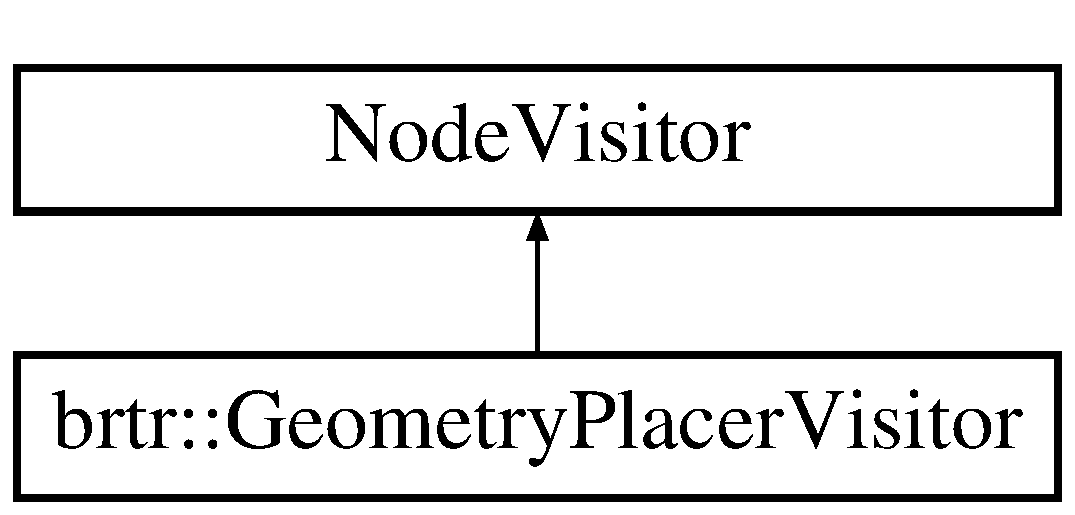
\includegraphics[height=2.000000cm]{classbrtr_1_1_geometry_placer_visitor}
\end{center}
\end{figure}
\subsection*{Public Member Functions}
\begin{DoxyCompactItemize}
\item 
\hyperlink{classbrtr_1_1_geometry_placer_visitor_a5e6ca74eba57f86c0916434cb38eb7fc}{Geometry\+Placer\+Visitor} (osg\+::\+Geometry $\ast$geometry\+To\+Place)
\begin{DoxyCompactList}\small\item\em Constructor. \end{DoxyCompactList}\item 
virtual void \hyperlink{classbrtr_1_1_geometry_placer_visitor_a26089587464d88953e38926162cb1c6e}{apply} (osg\+::\+Geode \&geode)
\begin{DoxyCompactList}\small\item\em Change the Geometry of this Geode. \end{DoxyCompactList}\item 
osg\+::ref\+\_\+ptr$<$ osg\+::\+Geometry $>$ \hyperlink{classbrtr_1_1_geometry_placer_visitor_ad784364cfe34434dc2183a5ead95db40}{get\+Geometry\+To\+Place} () const 
\item 
void \hyperlink{classbrtr_1_1_geometry_placer_visitor_a95e8e5c2df5b9a31949c55c796c90fd5}{set\+Geometry\+To\+Place} (osg\+::ref\+\_\+ptr$<$ osg\+::\+Geometry $>$ val)
\end{DoxyCompactItemize}
\subsection*{Private Attributes}
\begin{DoxyCompactItemize}
\item 
osg\+::ref\+\_\+ptr$<$ osg\+::\+Geometry $>$ \hyperlink{classbrtr_1_1_geometry_placer_visitor_a171826d64ddd04161d7525bc60faf045}{\+\_\+geometry\+To\+Place}
\end{DoxyCompactItemize}


\subsection{Detailed Description}
Node\+Visitor for batch replacing all Geometry in all visited Geodes. 

Takes a geometry as argument and replaces every geometry in the sub scene Useful for batch replacing a bunch of geometrys which were placed as dummys in Blender and then imported. Rotation and Scaling of the Geometry will persist. \begin{DoxyAuthor}{Author}
Gleb Ostrowski 
\end{DoxyAuthor}
\begin{DoxyVersion}{Version}
1.\+0 
\end{DoxyVersion}
\begin{DoxyDate}{Date}
2014 
\end{DoxyDate}
\begin{DoxyPrecond}{Precondition}
needs a Node which will accept it. Should have some Geode's for this to work 
\end{DoxyPrecond}
\begin{DoxyCopyright}{Copyright}
G\+N\+U Public License. 
\end{DoxyCopyright}


Definition at line \hyperlink{_geometry_placer_visitor_8h_source_l00015}{15} of file \hyperlink{_geometry_placer_visitor_8h_source}{Geometry\+Placer\+Visitor.\+h}.



\subsection{Constructor \& Destructor Documentation}
\hypertarget{classbrtr_1_1_geometry_placer_visitor_a5e6ca74eba57f86c0916434cb38eb7fc}{\index{brtr\+::\+Geometry\+Placer\+Visitor@{brtr\+::\+Geometry\+Placer\+Visitor}!Geometry\+Placer\+Visitor@{Geometry\+Placer\+Visitor}}
\index{Geometry\+Placer\+Visitor@{Geometry\+Placer\+Visitor}!brtr\+::\+Geometry\+Placer\+Visitor@{brtr\+::\+Geometry\+Placer\+Visitor}}
\subsubsection[{Geometry\+Placer\+Visitor}]{\setlength{\rightskip}{0pt plus 5cm}brtr\+::\+Geometry\+Placer\+Visitor\+::\+Geometry\+Placer\+Visitor (
\begin{DoxyParamCaption}
\item[{osg\+::\+Geometry $\ast$}]{geometry\+To\+Place}
\end{DoxyParamCaption}
)}}\label{classbrtr_1_1_geometry_placer_visitor_a5e6ca74eba57f86c0916434cb38eb7fc}


Constructor. 


\begin{DoxyParams}{Parameters}
{\em geometry\+To\+Place} & geometry to replace the found drawables \\
\hline
\end{DoxyParams}
\begin{DoxyReturn}{Returns}

\end{DoxyReturn}


Definition at line \hyperlink{_geometry_placer_visitor_8cpp_source_l00006}{6} of file \hyperlink{_geometry_placer_visitor_8cpp_source}{Geometry\+Placer\+Visitor.\+cpp}.



\subsection{Member Function Documentation}
\hypertarget{classbrtr_1_1_geometry_placer_visitor_a26089587464d88953e38926162cb1c6e}{\index{brtr\+::\+Geometry\+Placer\+Visitor@{brtr\+::\+Geometry\+Placer\+Visitor}!apply@{apply}}
\index{apply@{apply}!brtr\+::\+Geometry\+Placer\+Visitor@{brtr\+::\+Geometry\+Placer\+Visitor}}
\subsubsection[{apply}]{\setlength{\rightskip}{0pt plus 5cm}void brtr\+::\+Geometry\+Placer\+Visitor\+::apply (
\begin{DoxyParamCaption}
\item[{osg\+::\+Geode \&}]{geode}
\end{DoxyParamCaption}
)\hspace{0.3cm}{\ttfamily [virtual]}}}\label{classbrtr_1_1_geometry_placer_visitor_a26089587464d88953e38926162cb1c6e}


Change the Geometry of this Geode. 


\begin{DoxyParams}{Parameters}
{\em geode} & the Geode which will be alternate \\
\hline
\end{DoxyParams}


Definition at line \hyperlink{_geometry_placer_visitor_8cpp_source_l00011}{11} of file \hyperlink{_geometry_placer_visitor_8cpp_source}{Geometry\+Placer\+Visitor.\+cpp}.

\hypertarget{classbrtr_1_1_geometry_placer_visitor_ad784364cfe34434dc2183a5ead95db40}{\index{brtr\+::\+Geometry\+Placer\+Visitor@{brtr\+::\+Geometry\+Placer\+Visitor}!get\+Geometry\+To\+Place@{get\+Geometry\+To\+Place}}
\index{get\+Geometry\+To\+Place@{get\+Geometry\+To\+Place}!brtr\+::\+Geometry\+Placer\+Visitor@{brtr\+::\+Geometry\+Placer\+Visitor}}
\subsubsection[{get\+Geometry\+To\+Place}]{\setlength{\rightskip}{0pt plus 5cm}osg\+::ref\+\_\+ptr$<$ osg\+::\+Geometry $>$ brtr\+::\+Geometry\+Placer\+Visitor\+::get\+Geometry\+To\+Place (
\begin{DoxyParamCaption}
{}
\end{DoxyParamCaption}
) const}}\label{classbrtr_1_1_geometry_placer_visitor_ad784364cfe34434dc2183a5ead95db40}


Definition at line \hyperlink{_geometry_placer_visitor_8cpp_source_l00016}{16} of file \hyperlink{_geometry_placer_visitor_8cpp_source}{Geometry\+Placer\+Visitor.\+cpp}.

\hypertarget{classbrtr_1_1_geometry_placer_visitor_a95e8e5c2df5b9a31949c55c796c90fd5}{\index{brtr\+::\+Geometry\+Placer\+Visitor@{brtr\+::\+Geometry\+Placer\+Visitor}!set\+Geometry\+To\+Place@{set\+Geometry\+To\+Place}}
\index{set\+Geometry\+To\+Place@{set\+Geometry\+To\+Place}!brtr\+::\+Geometry\+Placer\+Visitor@{brtr\+::\+Geometry\+Placer\+Visitor}}
\subsubsection[{set\+Geometry\+To\+Place}]{\setlength{\rightskip}{0pt plus 5cm}void brtr\+::\+Geometry\+Placer\+Visitor\+::set\+Geometry\+To\+Place (
\begin{DoxyParamCaption}
\item[{osg\+::ref\+\_\+ptr$<$ osg\+::\+Geometry $>$}]{val}
\end{DoxyParamCaption}
)}}\label{classbrtr_1_1_geometry_placer_visitor_a95e8e5c2df5b9a31949c55c796c90fd5}


Definition at line \hyperlink{_geometry_placer_visitor_8cpp_source_l00020}{20} of file \hyperlink{_geometry_placer_visitor_8cpp_source}{Geometry\+Placer\+Visitor.\+cpp}.



\subsection{Member Data Documentation}
\hypertarget{classbrtr_1_1_geometry_placer_visitor_a171826d64ddd04161d7525bc60faf045}{\index{brtr\+::\+Geometry\+Placer\+Visitor@{brtr\+::\+Geometry\+Placer\+Visitor}!\+\_\+geometry\+To\+Place@{\+\_\+geometry\+To\+Place}}
\index{\+\_\+geometry\+To\+Place@{\+\_\+geometry\+To\+Place}!brtr\+::\+Geometry\+Placer\+Visitor@{brtr\+::\+Geometry\+Placer\+Visitor}}
\subsubsection[{\+\_\+geometry\+To\+Place}]{\setlength{\rightskip}{0pt plus 5cm}osg\+::ref\+\_\+ptr$<$osg\+::\+Geometry$>$ brtr\+::\+Geometry\+Placer\+Visitor\+::\+\_\+geometry\+To\+Place\hspace{0.3cm}{\ttfamily [private]}}}\label{classbrtr_1_1_geometry_placer_visitor_a171826d64ddd04161d7525bc60faf045}


Definition at line \hyperlink{_geometry_placer_visitor_8h_source_l00034}{34} of file \hyperlink{_geometry_placer_visitor_8h_source}{Geometry\+Placer\+Visitor.\+h}.



The documentation for this class was generated from the following files\+:\begin{DoxyCompactItemize}
\item 
header/\hyperlink{_geometry_placer_visitor_8h}{Geometry\+Placer\+Visitor.\+h}\item 
Util/\hyperlink{_geometry_placer_visitor_8cpp}{Geometry\+Placer\+Visitor.\+cpp}\end{DoxyCompactItemize}

\hypertarget{classbrtr_1_1_key_handler}{\section{brtr\+:\+:Key\+Handler Class Reference}
\label{classbrtr_1_1_key_handler}\index{brtr\+::\+Key\+Handler@{brtr\+::\+Key\+Handler}}
}


Key Handler Class, handles all of our Key\+Functions, which do not belong to camera control (this are handled by \hyperlink{classbrtr_1_1_f_p_s_camera_manipulator}{F\+P\+S\+Camera\+Manipulator})  




{\ttfamily \#include $<$Key\+Handler.\+h$>$}

Inheritance diagram for brtr\+:\+:Key\+Handler\+:\begin{figure}[H]
\begin{center}
\leavevmode
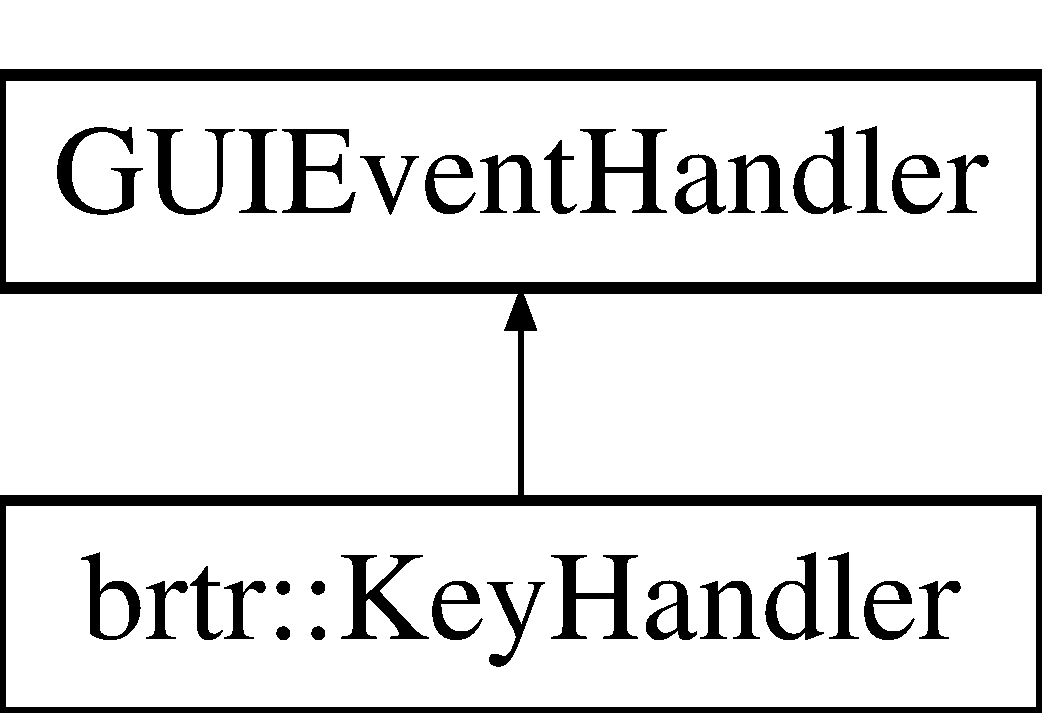
\includegraphics[height=2.000000cm]{classbrtr_1_1_key_handler}
\end{center}
\end{figure}
\subsection*{Public Member Functions}
\begin{DoxyCompactItemize}
\item 
\hyperlink{classbrtr_1_1_key_handler_aaae067fabc959780a9fae9c700c199da}{Key\+Handler} (osg\+::\+Node $\ast$, osg\+::\+Camera $\ast$post\+Process\+Cam, std\+::vector$<$ osg\+::ref\+\_\+ptr$<$ osg\+::\+Program $>$$>$ programs)
\begin{DoxyCompactList}\small\item\em Constructor. \end{DoxyCompactList}\item 
virtual bool \hyperlink{classbrtr_1_1_key_handler_a02df9f4339712d5b8b2b25b89048cf47}{handle} (const osg\+G\+A\+::\+G\+U\+I\+Event\+Adapter \&ea, osg\+G\+A\+::\+G\+U\+I\+Action\+Adapter \&aa)
\end{DoxyCompactItemize}
\subsection*{Protected Member Functions}
\begin{DoxyCompactItemize}
\item 
\hyperlink{classbrtr_1_1_key_handler_aabad0b142ba1d2e648069b4e8af17797}{$\sim$\+Key\+Handler} ()
\end{DoxyCompactItemize}
\subsection*{Private Member Functions}
\begin{DoxyCompactItemize}
\item 
bool \hyperlink{classbrtr_1_1_key_handler_a5af6a6e66e8754591b3425addc6e6858}{handle\+Key\+Down} (const osg\+G\+A\+::\+G\+U\+I\+Event\+Adapter \&ea, osg\+G\+A\+::\+G\+U\+I\+Action\+Adapter \&aa)
\item 
void \hyperlink{classbrtr_1_1_key_handler_a7f402d48b863ed19ef47038a32d1d05c}{mouse\+Intersection} (osg\+G\+A\+::\+G\+U\+I\+Action\+Adapter \&aa)
\begin{DoxyCompactList}\small\item\em Checks, if under the mouse (e.\+a center of screen) is an interact-\/able object (e.\+a geometry) \end{DoxyCompactList}\item 
\hyperlink{classbrtr_1_1_base_interaction_callback}{brtr\+::\+Base\+Interaction\+Callback} $\ast$ \hyperlink{classbrtr_1_1_key_handler_a1925fa114839192716167477714abfdc}{modify\+Text} (bool show)
\begin{DoxyCompactList}\small\item\em Shows the Interaction\+Message on screen, if there is an Interaction\+Object beneath the mouse (e.\+a center of screen) \end{DoxyCompactList}\end{DoxyCompactItemize}
\subsection*{Private Attributes}
\begin{DoxyCompactItemize}
\item 
osg\+::ref\+\_\+ptr$<$ osg\+::\+Drawable $>$ \hyperlink{classbrtr_1_1_key_handler_a4b0e380186a8172af6cf7c10dcff675a}{\+\_\+cur\+Drawable}
\item 
osg\+::ref\+\_\+ptr$<$ osg\+::\+Node $>$ \hyperlink{classbrtr_1_1_key_handler_a2ff68d9c79145d235f50fec1da625f99}{\+\_\+root\+Node}
\item 
osg\+::ref\+\_\+ptr$<$ osg\+::\+Polygon\+Mode $>$ \hyperlink{classbrtr_1_1_key_handler_a7aff4e23d4c614d8e0ccdc29a3c8882f}{\+\_\+wire\+Frame\+Mode}
\item 
osg\+::ref\+\_\+ptr$<$ osg\+::\+Polygon\+Mode $>$ \hyperlink{classbrtr_1_1_key_handler_ae210945e48748029cbea37fde7d601b5}{\+\_\+normale\+Mode}
\item 
osg\+::ref\+\_\+ptr$<$ osg\+::\+Camera $>$ \hyperlink{classbrtr_1_1_key_handler_aa4cc5f6ac9134e473f37968dfb1dd821}{\+\_\+post\+Process\+Cam}
\item 
std\+::vector$<$ osg\+::ref\+\_\+ptr\\*
$<$ osg\+::\+Program $>$ $>$ \hyperlink{classbrtr_1_1_key_handler_a492d086b9458475e595b3627a8dee0f9}{\+\_\+programs}
\item 
osg\+::ref\+\_\+ptr$<$ const \\*
osg\+G\+A\+::\+G\+U\+I\+Event\+Adapter $>$ \hyperlink{classbrtr_1_1_key_handler_a1b2404dcd19426a93d4474cd45da84e8}{\+\_\+mouse\+Event}
\item 
bool \hyperlink{classbrtr_1_1_key_handler_a6939e2c5e93e53d6090c999eae2fb927}{\+\_\+is\+Wire\+Frame}
\item 
unsigned int \hyperlink{classbrtr_1_1_key_handler_a578b374029e318a509983a01253a7736}{\+\_\+cur\+Prog}
\end{DoxyCompactItemize}


\subsection{Detailed Description}
Key Handler Class, handles all of our Key\+Functions, which do not belong to camera control (this are handled by \hyperlink{classbrtr_1_1_f_p_s_camera_manipulator}{F\+P\+S\+Camera\+Manipulator}) 

\begin{DoxyParagraph}{Controls\+: }

\begin{DoxyPre}
                   C       = Toggle WireFrame Mode On/Off
                 LClick    = Interact
                 Shift+1   = Toggle programs
             \end{DoxyPre}
 
\end{DoxyParagraph}
\begin{DoxyAuthor}{Author}
Gleb Ostrowski 
\end{DoxyAuthor}
\begin{DoxyVersion}{Version}
1.\+0 
\end{DoxyVersion}
\begin{DoxyDate}{Date}
2014 
\end{DoxyDate}
\begin{DoxyCopyright}{Copyright}
G\+N\+U Public License. 
\end{DoxyCopyright}


Definition at line \hyperlink{_key_handler_8h_source_l00023}{23} of file \hyperlink{_key_handler_8h_source}{Key\+Handler.\+h}.



\subsection{Constructor \& Destructor Documentation}
\hypertarget{classbrtr_1_1_key_handler_aaae067fabc959780a9fae9c700c199da}{\index{brtr\+::\+Key\+Handler@{brtr\+::\+Key\+Handler}!Key\+Handler@{Key\+Handler}}
\index{Key\+Handler@{Key\+Handler}!brtr\+::\+Key\+Handler@{brtr\+::\+Key\+Handler}}
\subsubsection[{Key\+Handler}]{\setlength{\rightskip}{0pt plus 5cm}brtr\+::\+Key\+Handler\+::\+Key\+Handler (
\begin{DoxyParamCaption}
\item[{osg\+::\+Node $\ast$}]{root\+Node, }
\item[{osg\+::\+Camera $\ast$}]{post\+Process\+Cam, }
\item[{std\+::vector$<$ osg\+::ref\+\_\+ptr$<$ osg\+::\+Program $>$$>$}]{programs}
\end{DoxyParamCaption}
)}}\label{classbrtr_1_1_key_handler_aaae067fabc959780a9fae9c700c199da}


Constructor. 


\begin{DoxyParams}{Parameters}
{\em rootnode} & rootnode of the scene, polygonmode will be activatd on all children \\
\hline
{\em post\+Process\+Cam} & node containing the postprocess programs \\
\hline
{\em programs} & vector with postprocess programs \\
\hline
\end{DoxyParams}


Definition at line \hyperlink{_key_handler_8cpp_source_l00008}{8} of file \hyperlink{_key_handler_8cpp_source}{Key\+Handler.\+cpp}.

\hypertarget{classbrtr_1_1_key_handler_aabad0b142ba1d2e648069b4e8af17797}{\index{brtr\+::\+Key\+Handler@{brtr\+::\+Key\+Handler}!````~Key\+Handler@{$\sim$\+Key\+Handler}}
\index{````~Key\+Handler@{$\sim$\+Key\+Handler}!brtr\+::\+Key\+Handler@{brtr\+::\+Key\+Handler}}
\subsubsection[{$\sim$\+Key\+Handler}]{\setlength{\rightskip}{0pt plus 5cm}brtr\+::\+Key\+Handler\+::$\sim$\+Key\+Handler (
\begin{DoxyParamCaption}
{}
\end{DoxyParamCaption}
)\hspace{0.3cm}{\ttfamily [protected]}}}\label{classbrtr_1_1_key_handler_aabad0b142ba1d2e648069b4e8af17797}


Definition at line \hyperlink{_key_handler_8cpp_source_l00019}{19} of file \hyperlink{_key_handler_8cpp_source}{Key\+Handler.\+cpp}.



\subsection{Member Function Documentation}
\hypertarget{classbrtr_1_1_key_handler_a02df9f4339712d5b8b2b25b89048cf47}{\index{brtr\+::\+Key\+Handler@{brtr\+::\+Key\+Handler}!handle@{handle}}
\index{handle@{handle}!brtr\+::\+Key\+Handler@{brtr\+::\+Key\+Handler}}
\subsubsection[{handle}]{\setlength{\rightskip}{0pt plus 5cm}bool brtr\+::\+Key\+Handler\+::handle (
\begin{DoxyParamCaption}
\item[{const osg\+G\+A\+::\+G\+U\+I\+Event\+Adapter \&}]{ea, }
\item[{osg\+G\+A\+::\+G\+U\+I\+Action\+Adapter \&}]{aa}
\end{DoxyParamCaption}
)\hspace{0.3cm}{\ttfamily [virtual]}}}\label{classbrtr_1_1_key_handler_a02df9f4339712d5b8b2b25b89048cf47}


Definition at line \hyperlink{_key_handler_8cpp_source_l00021}{21} of file \hyperlink{_key_handler_8cpp_source}{Key\+Handler.\+cpp}.

\hypertarget{classbrtr_1_1_key_handler_a5af6a6e66e8754591b3425addc6e6858}{\index{brtr\+::\+Key\+Handler@{brtr\+::\+Key\+Handler}!handle\+Key\+Down@{handle\+Key\+Down}}
\index{handle\+Key\+Down@{handle\+Key\+Down}!brtr\+::\+Key\+Handler@{brtr\+::\+Key\+Handler}}
\subsubsection[{handle\+Key\+Down}]{\setlength{\rightskip}{0pt plus 5cm}bool brtr\+::\+Key\+Handler\+::handle\+Key\+Down (
\begin{DoxyParamCaption}
\item[{const osg\+G\+A\+::\+G\+U\+I\+Event\+Adapter \&}]{ea, }
\item[{osg\+G\+A\+::\+G\+U\+I\+Action\+Adapter \&}]{aa}
\end{DoxyParamCaption}
)\hspace{0.3cm}{\ttfamily [private]}}}\label{classbrtr_1_1_key_handler_a5af6a6e66e8754591b3425addc6e6858}


Definition at line \hyperlink{_key_handler_8cpp_source_l00053}{53} of file \hyperlink{_key_handler_8cpp_source}{Key\+Handler.\+cpp}.

\hypertarget{classbrtr_1_1_key_handler_a1925fa114839192716167477714abfdc}{\index{brtr\+::\+Key\+Handler@{brtr\+::\+Key\+Handler}!modify\+Text@{modify\+Text}}
\index{modify\+Text@{modify\+Text}!brtr\+::\+Key\+Handler@{brtr\+::\+Key\+Handler}}
\subsubsection[{modify\+Text}]{\setlength{\rightskip}{0pt plus 5cm}{\bf brtr\+::\+Base\+Interaction\+Callback} $\ast$ brtr\+::\+Key\+Handler\+::modify\+Text (
\begin{DoxyParamCaption}
\item[{bool}]{show}
\end{DoxyParamCaption}
)\hspace{0.3cm}{\ttfamily [private]}}}\label{classbrtr_1_1_key_handler_a1925fa114839192716167477714abfdc}


Shows the Interaction\+Message on screen, if there is an Interaction\+Object beneath the mouse (e.\+a center of screen) 


\begin{DoxyParams}{Parameters}
{\em to} & show or not show the text, that is the question \\
\hline
\end{DoxyParams}
\begin{DoxyReturn}{Returns}
the \hyperlink{classbrtr_1_1_base_interaction_callback}{Base\+Interaction\+Callback} associated with the interaction\+Object, if any, null else; 
\end{DoxyReturn}


Definition at line \hyperlink{_key_handler_8cpp_source_l00101}{101} of file \hyperlink{_key_handler_8cpp_source}{Key\+Handler.\+cpp}.

\hypertarget{classbrtr_1_1_key_handler_a7f402d48b863ed19ef47038a32d1d05c}{\index{brtr\+::\+Key\+Handler@{brtr\+::\+Key\+Handler}!mouse\+Intersection@{mouse\+Intersection}}
\index{mouse\+Intersection@{mouse\+Intersection}!brtr\+::\+Key\+Handler@{brtr\+::\+Key\+Handler}}
\subsubsection[{mouse\+Intersection}]{\setlength{\rightskip}{0pt plus 5cm}void brtr\+::\+Key\+Handler\+::mouse\+Intersection (
\begin{DoxyParamCaption}
\item[{osg\+G\+A\+::\+G\+U\+I\+Action\+Adapter \&}]{aa}
\end{DoxyParamCaption}
)\hspace{0.3cm}{\ttfamily [private]}}}\label{classbrtr_1_1_key_handler_a7f402d48b863ed19ef47038a32d1d05c}


Checks, if under the mouse (e.\+a center of screen) is an interact-\/able object (e.\+a geometry) 


\begin{DoxyParams}{Parameters}
{\em aa} & G\+U\+I\+Action\+Adapter for getting the camera , to whom the Line\+Intersection\+Visitor will be attached to \\
\hline
\end{DoxyParams}


Definition at line \hyperlink{_key_handler_8cpp_source_l00076}{76} of file \hyperlink{_key_handler_8cpp_source}{Key\+Handler.\+cpp}.



\subsection{Member Data Documentation}
\hypertarget{classbrtr_1_1_key_handler_a4b0e380186a8172af6cf7c10dcff675a}{\index{brtr\+::\+Key\+Handler@{brtr\+::\+Key\+Handler}!\+\_\+cur\+Drawable@{\+\_\+cur\+Drawable}}
\index{\+\_\+cur\+Drawable@{\+\_\+cur\+Drawable}!brtr\+::\+Key\+Handler@{brtr\+::\+Key\+Handler}}
\subsubsection[{\+\_\+cur\+Drawable}]{\setlength{\rightskip}{0pt plus 5cm}osg\+::ref\+\_\+ptr$<$osg\+::\+Drawable$>$ brtr\+::\+Key\+Handler\+::\+\_\+cur\+Drawable\hspace{0.3cm}{\ttfamily [private]}}}\label{classbrtr_1_1_key_handler_a4b0e380186a8172af6cf7c10dcff675a}


Definition at line \hyperlink{_key_handler_8h_source_l00053}{53} of file \hyperlink{_key_handler_8h_source}{Key\+Handler.\+h}.

\hypertarget{classbrtr_1_1_key_handler_a578b374029e318a509983a01253a7736}{\index{brtr\+::\+Key\+Handler@{brtr\+::\+Key\+Handler}!\+\_\+cur\+Prog@{\+\_\+cur\+Prog}}
\index{\+\_\+cur\+Prog@{\+\_\+cur\+Prog}!brtr\+::\+Key\+Handler@{brtr\+::\+Key\+Handler}}
\subsubsection[{\+\_\+cur\+Prog}]{\setlength{\rightskip}{0pt plus 5cm}unsigned int brtr\+::\+Key\+Handler\+::\+\_\+cur\+Prog\hspace{0.3cm}{\ttfamily [private]}}}\label{classbrtr_1_1_key_handler_a578b374029e318a509983a01253a7736}


Definition at line \hyperlink{_key_handler_8h_source_l00061}{61} of file \hyperlink{_key_handler_8h_source}{Key\+Handler.\+h}.

\hypertarget{classbrtr_1_1_key_handler_a6939e2c5e93e53d6090c999eae2fb927}{\index{brtr\+::\+Key\+Handler@{brtr\+::\+Key\+Handler}!\+\_\+is\+Wire\+Frame@{\+\_\+is\+Wire\+Frame}}
\index{\+\_\+is\+Wire\+Frame@{\+\_\+is\+Wire\+Frame}!brtr\+::\+Key\+Handler@{brtr\+::\+Key\+Handler}}
\subsubsection[{\+\_\+is\+Wire\+Frame}]{\setlength{\rightskip}{0pt plus 5cm}bool brtr\+::\+Key\+Handler\+::\+\_\+is\+Wire\+Frame\hspace{0.3cm}{\ttfamily [private]}}}\label{classbrtr_1_1_key_handler_a6939e2c5e93e53d6090c999eae2fb927}


Definition at line \hyperlink{_key_handler_8h_source_l00060}{60} of file \hyperlink{_key_handler_8h_source}{Key\+Handler.\+h}.

\hypertarget{classbrtr_1_1_key_handler_a1b2404dcd19426a93d4474cd45da84e8}{\index{brtr\+::\+Key\+Handler@{brtr\+::\+Key\+Handler}!\+\_\+mouse\+Event@{\+\_\+mouse\+Event}}
\index{\+\_\+mouse\+Event@{\+\_\+mouse\+Event}!brtr\+::\+Key\+Handler@{brtr\+::\+Key\+Handler}}
\subsubsection[{\+\_\+mouse\+Event}]{\setlength{\rightskip}{0pt plus 5cm}osg\+::ref\+\_\+ptr$<$ const osg\+G\+A\+::\+G\+U\+I\+Event\+Adapter $>$ brtr\+::\+Key\+Handler\+::\+\_\+mouse\+Event\hspace{0.3cm}{\ttfamily [private]}}}\label{classbrtr_1_1_key_handler_a1b2404dcd19426a93d4474cd45da84e8}


Definition at line \hyperlink{_key_handler_8h_source_l00059}{59} of file \hyperlink{_key_handler_8h_source}{Key\+Handler.\+h}.

\hypertarget{classbrtr_1_1_key_handler_ae210945e48748029cbea37fde7d601b5}{\index{brtr\+::\+Key\+Handler@{brtr\+::\+Key\+Handler}!\+\_\+normale\+Mode@{\+\_\+normale\+Mode}}
\index{\+\_\+normale\+Mode@{\+\_\+normale\+Mode}!brtr\+::\+Key\+Handler@{brtr\+::\+Key\+Handler}}
\subsubsection[{\+\_\+normale\+Mode}]{\setlength{\rightskip}{0pt plus 5cm}osg\+::ref\+\_\+ptr$<$osg\+::\+Polygon\+Mode$>$ brtr\+::\+Key\+Handler\+::\+\_\+normale\+Mode\hspace{0.3cm}{\ttfamily [private]}}}\label{classbrtr_1_1_key_handler_ae210945e48748029cbea37fde7d601b5}


Definition at line \hyperlink{_key_handler_8h_source_l00056}{56} of file \hyperlink{_key_handler_8h_source}{Key\+Handler.\+h}.

\hypertarget{classbrtr_1_1_key_handler_aa4cc5f6ac9134e473f37968dfb1dd821}{\index{brtr\+::\+Key\+Handler@{brtr\+::\+Key\+Handler}!\+\_\+post\+Process\+Cam@{\+\_\+post\+Process\+Cam}}
\index{\+\_\+post\+Process\+Cam@{\+\_\+post\+Process\+Cam}!brtr\+::\+Key\+Handler@{brtr\+::\+Key\+Handler}}
\subsubsection[{\+\_\+post\+Process\+Cam}]{\setlength{\rightskip}{0pt plus 5cm}osg\+::ref\+\_\+ptr$<$osg\+::\+Camera$>$ brtr\+::\+Key\+Handler\+::\+\_\+post\+Process\+Cam\hspace{0.3cm}{\ttfamily [private]}}}\label{classbrtr_1_1_key_handler_aa4cc5f6ac9134e473f37968dfb1dd821}


Definition at line \hyperlink{_key_handler_8h_source_l00057}{57} of file \hyperlink{_key_handler_8h_source}{Key\+Handler.\+h}.

\hypertarget{classbrtr_1_1_key_handler_a492d086b9458475e595b3627a8dee0f9}{\index{brtr\+::\+Key\+Handler@{brtr\+::\+Key\+Handler}!\+\_\+programs@{\+\_\+programs}}
\index{\+\_\+programs@{\+\_\+programs}!brtr\+::\+Key\+Handler@{brtr\+::\+Key\+Handler}}
\subsubsection[{\+\_\+programs}]{\setlength{\rightskip}{0pt plus 5cm}std\+::vector$<$osg\+::ref\+\_\+ptr$<$osg\+::\+Program$>$ $>$ brtr\+::\+Key\+Handler\+::\+\_\+programs\hspace{0.3cm}{\ttfamily [private]}}}\label{classbrtr_1_1_key_handler_a492d086b9458475e595b3627a8dee0f9}


Definition at line \hyperlink{_key_handler_8h_source_l00058}{58} of file \hyperlink{_key_handler_8h_source}{Key\+Handler.\+h}.

\hypertarget{classbrtr_1_1_key_handler_a2ff68d9c79145d235f50fec1da625f99}{\index{brtr\+::\+Key\+Handler@{brtr\+::\+Key\+Handler}!\+\_\+root\+Node@{\+\_\+root\+Node}}
\index{\+\_\+root\+Node@{\+\_\+root\+Node}!brtr\+::\+Key\+Handler@{brtr\+::\+Key\+Handler}}
\subsubsection[{\+\_\+root\+Node}]{\setlength{\rightskip}{0pt plus 5cm}osg\+::ref\+\_\+ptr$<$osg\+::\+Node$>$ brtr\+::\+Key\+Handler\+::\+\_\+root\+Node\hspace{0.3cm}{\ttfamily [private]}}}\label{classbrtr_1_1_key_handler_a2ff68d9c79145d235f50fec1da625f99}


Definition at line \hyperlink{_key_handler_8h_source_l00054}{54} of file \hyperlink{_key_handler_8h_source}{Key\+Handler.\+h}.

\hypertarget{classbrtr_1_1_key_handler_a7aff4e23d4c614d8e0ccdc29a3c8882f}{\index{brtr\+::\+Key\+Handler@{brtr\+::\+Key\+Handler}!\+\_\+wire\+Frame\+Mode@{\+\_\+wire\+Frame\+Mode}}
\index{\+\_\+wire\+Frame\+Mode@{\+\_\+wire\+Frame\+Mode}!brtr\+::\+Key\+Handler@{brtr\+::\+Key\+Handler}}
\subsubsection[{\+\_\+wire\+Frame\+Mode}]{\setlength{\rightskip}{0pt plus 5cm}osg\+::ref\+\_\+ptr$<$osg\+::\+Polygon\+Mode$>$ brtr\+::\+Key\+Handler\+::\+\_\+wire\+Frame\+Mode\hspace{0.3cm}{\ttfamily [private]}}}\label{classbrtr_1_1_key_handler_a7aff4e23d4c614d8e0ccdc29a3c8882f}


Definition at line \hyperlink{_key_handler_8h_source_l00055}{55} of file \hyperlink{_key_handler_8h_source}{Key\+Handler.\+h}.



The documentation for this class was generated from the following files\+:\begin{DoxyCompactItemize}
\item 
header/\hyperlink{_key_handler_8h}{Key\+Handler.\+h}\item 
G\+U\+I/\hyperlink{_key_handler_8cpp}{Key\+Handler.\+cpp}\end{DoxyCompactItemize}

\hypertarget{classbrtr_1_1_modify_material_visitor}{\section{brtr\+:\+:Modify\+Material\+Visitor Class Reference}
\label{classbrtr_1_1_modify_material_visitor}\index{brtr\+::\+Modify\+Material\+Visitor@{brtr\+::\+Modify\+Material\+Visitor}}
}


Visitor for altering the material attributes, mainly used for objects craeted with blender.  




{\ttfamily \#include $<$Modify\+Material\+Visitor.\+h$>$}

Inheritance diagram for brtr\+:\+:Modify\+Material\+Visitor\+:\begin{figure}[H]
\begin{center}
\leavevmode
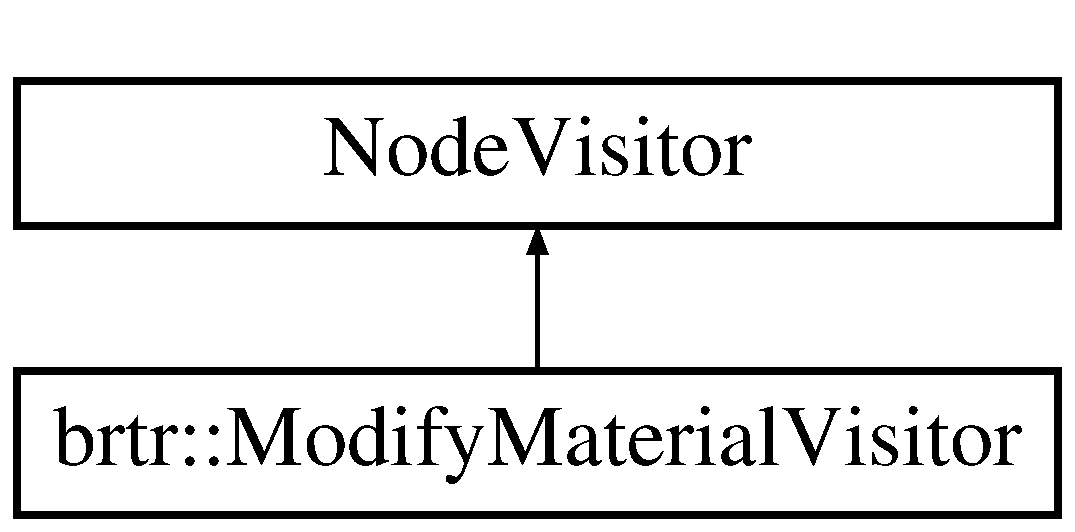
\includegraphics[height=2.000000cm]{classbrtr_1_1_modify_material_visitor}
\end{center}
\end{figure}
\subsection*{Public Member Functions}
\begin{DoxyCompactItemize}
\item 
\hyperlink{classbrtr_1_1_modify_material_visitor_a240eed8002f7c81d8cd63aaaf4037381}{Modify\+Material\+Visitor} ()
\item 
void \hyperlink{classbrtr_1_1_modify_material_visitor_a74bf42fdfffbc1f7d433c1199f563ccb}{apply} (osg\+::\+Geode \&geode)
\item 
osg\+::\+Vec4 \hyperlink{classbrtr_1_1_modify_material_visitor_ac79c5aeaa29e381e46e130c088966ad9}{get\+Diffuse} () const 
\item 
\hyperlink{classbrtr_1_1_modify_material_visitor}{Modify\+Material\+Visitor} \& \hyperlink{classbrtr_1_1_modify_material_visitor_a17748f6a7f41431832da66dd65e1c41f}{set\+Diffuse} (osg\+::\+Vec4 val)
\item 
osg\+::\+Vec4 \hyperlink{classbrtr_1_1_modify_material_visitor_a5be2b7553a9ecbe1c6d50425119f7e9e}{get\+Specular} () const 
\item 
\hyperlink{classbrtr_1_1_modify_material_visitor}{Modify\+Material\+Visitor} \& \hyperlink{classbrtr_1_1_modify_material_visitor_a7a8a5a938799c5193645d86aa6dc6a7c}{set\+Specular} (osg\+::\+Vec4 val)
\item 
osg\+::\+Vec4 \hyperlink{classbrtr_1_1_modify_material_visitor_a2a87910d4f316359eb6bf75620edf947}{get\+Ambient} () const 
\item 
\hyperlink{classbrtr_1_1_modify_material_visitor}{Modify\+Material\+Visitor} \& \hyperlink{classbrtr_1_1_modify_material_visitor_adfaa00524e765fdf3ddc5968187623cd}{set\+Ambient} (osg\+::\+Vec4 val)
\item 
double \hyperlink{classbrtr_1_1_modify_material_visitor_a68f37fe264bd8f51e1d7a37f8048b103}{get\+Shininess} () const 
\item 
\hyperlink{classbrtr_1_1_modify_material_visitor}{Modify\+Material\+Visitor} \& \hyperlink{classbrtr_1_1_modify_material_visitor_a698aa0c31f8c5add503d47bc9898eec3}{set\+Shininess} (double val)
\end{DoxyCompactItemize}
\subsection*{Private Attributes}
\begin{DoxyCompactItemize}
\item 
osg\+::\+Vec4 \hyperlink{classbrtr_1_1_modify_material_visitor_a33e06870644e892df2ac9af4c5bbfbd8}{\+\_\+diffuse}
\item 
osg\+::\+Vec4 \hyperlink{classbrtr_1_1_modify_material_visitor_a4cbbdf6ecd85ec563839545fc328fbfe}{\+\_\+specular}
\item 
osg\+::\+Vec4 \hyperlink{classbrtr_1_1_modify_material_visitor_a1cffff6daf689c23a4e9680cd8f1441b}{\+\_\+ambient}
\item 
double \hyperlink{classbrtr_1_1_modify_material_visitor_a297f5208848d0bba92653bbd15908f68}{\+\_\+shininess}
\item 
bool \hyperlink{classbrtr_1_1_modify_material_visitor_a351e4cfeca41aa6f746956661930f994}{\+\_\+ambient\+Flag}
\item 
bool \hyperlink{classbrtr_1_1_modify_material_visitor_a154ad99cb3796be6d04347cdbfb66e10}{\+\_\+specular\+Flag}
\item 
bool \hyperlink{classbrtr_1_1_modify_material_visitor_a8b30ec1a8b93422fc168597a47425041}{\+\_\+shininess\+Flag}
\item 
bool \hyperlink{classbrtr_1_1_modify_material_visitor_a511c43fcd16d68855e6e63ca3ec1a84e}{\+\_\+diffuse\+Flag}
\end{DoxyCompactItemize}


\subsection{Detailed Description}
Visitor for altering the material attributes, mainly used for objects craeted with blender. 

before applying one must set the desired changes (set\+Diffuse, set\+Ambient, set\+Specular oder set\+Shininess) \begin{DoxyAuthor}{Author}
Gleb Ostrowski 
\end{DoxyAuthor}
\begin{DoxyVersion}{Version}
1.\+0 
\end{DoxyVersion}
\begin{DoxyDate}{Date}
2014 
\end{DoxyDate}
\begin{DoxyCopyright}{Copyright}
G\+N\+U Public License. 
\end{DoxyCopyright}


Definition at line \hyperlink{_modify_material_visitor_8h_source_l00014}{14} of file \hyperlink{_modify_material_visitor_8h_source}{Modify\+Material\+Visitor.\+h}.



\subsection{Constructor \& Destructor Documentation}
\hypertarget{classbrtr_1_1_modify_material_visitor_a240eed8002f7c81d8cd63aaaf4037381}{\index{brtr\+::\+Modify\+Material\+Visitor@{brtr\+::\+Modify\+Material\+Visitor}!Modify\+Material\+Visitor@{Modify\+Material\+Visitor}}
\index{Modify\+Material\+Visitor@{Modify\+Material\+Visitor}!brtr\+::\+Modify\+Material\+Visitor@{brtr\+::\+Modify\+Material\+Visitor}}
\subsubsection[{Modify\+Material\+Visitor}]{\setlength{\rightskip}{0pt plus 5cm}brtr\+::\+Modify\+Material\+Visitor\+::\+Modify\+Material\+Visitor (
\begin{DoxyParamCaption}
{}
\end{DoxyParamCaption}
)}}\label{classbrtr_1_1_modify_material_visitor_a240eed8002f7c81d8cd63aaaf4037381}


Definition at line \hyperlink{_modify_material_visitor_8cpp_source_l00005}{5} of file \hyperlink{_modify_material_visitor_8cpp_source}{Modify\+Material\+Visitor.\+cpp}.



\subsection{Member Function Documentation}
\hypertarget{classbrtr_1_1_modify_material_visitor_a74bf42fdfffbc1f7d433c1199f563ccb}{\index{brtr\+::\+Modify\+Material\+Visitor@{brtr\+::\+Modify\+Material\+Visitor}!apply@{apply}}
\index{apply@{apply}!brtr\+::\+Modify\+Material\+Visitor@{brtr\+::\+Modify\+Material\+Visitor}}
\subsubsection[{apply}]{\setlength{\rightskip}{0pt plus 5cm}void brtr\+::\+Modify\+Material\+Visitor\+::apply (
\begin{DoxyParamCaption}
\item[{osg\+::\+Geode \&}]{geode}
\end{DoxyParamCaption}
)}}\label{classbrtr_1_1_modify_material_visitor_a74bf42fdfffbc1f7d433c1199f563ccb}


Definition at line \hyperlink{_modify_material_visitor_8cpp_source_l00014}{14} of file \hyperlink{_modify_material_visitor_8cpp_source}{Modify\+Material\+Visitor.\+cpp}.

\hypertarget{classbrtr_1_1_modify_material_visitor_a2a87910d4f316359eb6bf75620edf947}{\index{brtr\+::\+Modify\+Material\+Visitor@{brtr\+::\+Modify\+Material\+Visitor}!get\+Ambient@{get\+Ambient}}
\index{get\+Ambient@{get\+Ambient}!brtr\+::\+Modify\+Material\+Visitor@{brtr\+::\+Modify\+Material\+Visitor}}
\subsubsection[{get\+Ambient}]{\setlength{\rightskip}{0pt plus 5cm}osg\+::\+Vec4 brtr\+::\+Modify\+Material\+Visitor\+::get\+Ambient (
\begin{DoxyParamCaption}
{}
\end{DoxyParamCaption}
) const}}\label{classbrtr_1_1_modify_material_visitor_a2a87910d4f316359eb6bf75620edf947}


Definition at line \hyperlink{_modify_material_visitor_8cpp_source_l00053}{53} of file \hyperlink{_modify_material_visitor_8cpp_source}{Modify\+Material\+Visitor.\+cpp}.

\hypertarget{classbrtr_1_1_modify_material_visitor_ac79c5aeaa29e381e46e130c088966ad9}{\index{brtr\+::\+Modify\+Material\+Visitor@{brtr\+::\+Modify\+Material\+Visitor}!get\+Diffuse@{get\+Diffuse}}
\index{get\+Diffuse@{get\+Diffuse}!brtr\+::\+Modify\+Material\+Visitor@{brtr\+::\+Modify\+Material\+Visitor}}
\subsubsection[{get\+Diffuse}]{\setlength{\rightskip}{0pt plus 5cm}osg\+::\+Vec4 brtr\+::\+Modify\+Material\+Visitor\+::get\+Diffuse (
\begin{DoxyParamCaption}
{}
\end{DoxyParamCaption}
) const}}\label{classbrtr_1_1_modify_material_visitor_ac79c5aeaa29e381e46e130c088966ad9}


Definition at line \hyperlink{_modify_material_visitor_8cpp_source_l00033}{33} of file \hyperlink{_modify_material_visitor_8cpp_source}{Modify\+Material\+Visitor.\+cpp}.

\hypertarget{classbrtr_1_1_modify_material_visitor_a68f37fe264bd8f51e1d7a37f8048b103}{\index{brtr\+::\+Modify\+Material\+Visitor@{brtr\+::\+Modify\+Material\+Visitor}!get\+Shininess@{get\+Shininess}}
\index{get\+Shininess@{get\+Shininess}!brtr\+::\+Modify\+Material\+Visitor@{brtr\+::\+Modify\+Material\+Visitor}}
\subsubsection[{get\+Shininess}]{\setlength{\rightskip}{0pt plus 5cm}double brtr\+::\+Modify\+Material\+Visitor\+::get\+Shininess (
\begin{DoxyParamCaption}
{}
\end{DoxyParamCaption}
) const}}\label{classbrtr_1_1_modify_material_visitor_a68f37fe264bd8f51e1d7a37f8048b103}


Definition at line \hyperlink{_modify_material_visitor_8cpp_source_l00063}{63} of file \hyperlink{_modify_material_visitor_8cpp_source}{Modify\+Material\+Visitor.\+cpp}.

\hypertarget{classbrtr_1_1_modify_material_visitor_a5be2b7553a9ecbe1c6d50425119f7e9e}{\index{brtr\+::\+Modify\+Material\+Visitor@{brtr\+::\+Modify\+Material\+Visitor}!get\+Specular@{get\+Specular}}
\index{get\+Specular@{get\+Specular}!brtr\+::\+Modify\+Material\+Visitor@{brtr\+::\+Modify\+Material\+Visitor}}
\subsubsection[{get\+Specular}]{\setlength{\rightskip}{0pt plus 5cm}osg\+::\+Vec4 brtr\+::\+Modify\+Material\+Visitor\+::get\+Specular (
\begin{DoxyParamCaption}
{}
\end{DoxyParamCaption}
) const}}\label{classbrtr_1_1_modify_material_visitor_a5be2b7553a9ecbe1c6d50425119f7e9e}


Definition at line \hyperlink{_modify_material_visitor_8cpp_source_l00043}{43} of file \hyperlink{_modify_material_visitor_8cpp_source}{Modify\+Material\+Visitor.\+cpp}.

\hypertarget{classbrtr_1_1_modify_material_visitor_adfaa00524e765fdf3ddc5968187623cd}{\index{brtr\+::\+Modify\+Material\+Visitor@{brtr\+::\+Modify\+Material\+Visitor}!set\+Ambient@{set\+Ambient}}
\index{set\+Ambient@{set\+Ambient}!brtr\+::\+Modify\+Material\+Visitor@{brtr\+::\+Modify\+Material\+Visitor}}
\subsubsection[{set\+Ambient}]{\setlength{\rightskip}{0pt plus 5cm}{\bf Modify\+Material\+Visitor} \& brtr\+::\+Modify\+Material\+Visitor\+::set\+Ambient (
\begin{DoxyParamCaption}
\item[{osg\+::\+Vec4}]{val}
\end{DoxyParamCaption}
)}}\label{classbrtr_1_1_modify_material_visitor_adfaa00524e765fdf3ddc5968187623cd}


Definition at line \hyperlink{_modify_material_visitor_8cpp_source_l00057}{57} of file \hyperlink{_modify_material_visitor_8cpp_source}{Modify\+Material\+Visitor.\+cpp}.

\hypertarget{classbrtr_1_1_modify_material_visitor_a17748f6a7f41431832da66dd65e1c41f}{\index{brtr\+::\+Modify\+Material\+Visitor@{brtr\+::\+Modify\+Material\+Visitor}!set\+Diffuse@{set\+Diffuse}}
\index{set\+Diffuse@{set\+Diffuse}!brtr\+::\+Modify\+Material\+Visitor@{brtr\+::\+Modify\+Material\+Visitor}}
\subsubsection[{set\+Diffuse}]{\setlength{\rightskip}{0pt plus 5cm}{\bf Modify\+Material\+Visitor} \& brtr\+::\+Modify\+Material\+Visitor\+::set\+Diffuse (
\begin{DoxyParamCaption}
\item[{osg\+::\+Vec4}]{val}
\end{DoxyParamCaption}
)}}\label{classbrtr_1_1_modify_material_visitor_a17748f6a7f41431832da66dd65e1c41f}


Definition at line \hyperlink{_modify_material_visitor_8cpp_source_l00037}{37} of file \hyperlink{_modify_material_visitor_8cpp_source}{Modify\+Material\+Visitor.\+cpp}.

\hypertarget{classbrtr_1_1_modify_material_visitor_a698aa0c31f8c5add503d47bc9898eec3}{\index{brtr\+::\+Modify\+Material\+Visitor@{brtr\+::\+Modify\+Material\+Visitor}!set\+Shininess@{set\+Shininess}}
\index{set\+Shininess@{set\+Shininess}!brtr\+::\+Modify\+Material\+Visitor@{brtr\+::\+Modify\+Material\+Visitor}}
\subsubsection[{set\+Shininess}]{\setlength{\rightskip}{0pt plus 5cm}{\bf Modify\+Material\+Visitor} \& brtr\+::\+Modify\+Material\+Visitor\+::set\+Shininess (
\begin{DoxyParamCaption}
\item[{double}]{val}
\end{DoxyParamCaption}
)}}\label{classbrtr_1_1_modify_material_visitor_a698aa0c31f8c5add503d47bc9898eec3}


Definition at line \hyperlink{_modify_material_visitor_8cpp_source_l00067}{67} of file \hyperlink{_modify_material_visitor_8cpp_source}{Modify\+Material\+Visitor.\+cpp}.

\hypertarget{classbrtr_1_1_modify_material_visitor_a7a8a5a938799c5193645d86aa6dc6a7c}{\index{brtr\+::\+Modify\+Material\+Visitor@{brtr\+::\+Modify\+Material\+Visitor}!set\+Specular@{set\+Specular}}
\index{set\+Specular@{set\+Specular}!brtr\+::\+Modify\+Material\+Visitor@{brtr\+::\+Modify\+Material\+Visitor}}
\subsubsection[{set\+Specular}]{\setlength{\rightskip}{0pt plus 5cm}{\bf Modify\+Material\+Visitor} \& brtr\+::\+Modify\+Material\+Visitor\+::set\+Specular (
\begin{DoxyParamCaption}
\item[{osg\+::\+Vec4}]{val}
\end{DoxyParamCaption}
)}}\label{classbrtr_1_1_modify_material_visitor_a7a8a5a938799c5193645d86aa6dc6a7c}


Definition at line \hyperlink{_modify_material_visitor_8cpp_source_l00047}{47} of file \hyperlink{_modify_material_visitor_8cpp_source}{Modify\+Material\+Visitor.\+cpp}.



\subsection{Member Data Documentation}
\hypertarget{classbrtr_1_1_modify_material_visitor_a1cffff6daf689c23a4e9680cd8f1441b}{\index{brtr\+::\+Modify\+Material\+Visitor@{brtr\+::\+Modify\+Material\+Visitor}!\+\_\+ambient@{\+\_\+ambient}}
\index{\+\_\+ambient@{\+\_\+ambient}!brtr\+::\+Modify\+Material\+Visitor@{brtr\+::\+Modify\+Material\+Visitor}}
\subsubsection[{\+\_\+ambient}]{\setlength{\rightskip}{0pt plus 5cm}osg\+::\+Vec4 brtr\+::\+Modify\+Material\+Visitor\+::\+\_\+ambient\hspace{0.3cm}{\ttfamily [private]}}}\label{classbrtr_1_1_modify_material_visitor_a1cffff6daf689c23a4e9680cd8f1441b}


Definition at line \hyperlink{_modify_material_visitor_8h_source_l00031}{31} of file \hyperlink{_modify_material_visitor_8h_source}{Modify\+Material\+Visitor.\+h}.

\hypertarget{classbrtr_1_1_modify_material_visitor_a351e4cfeca41aa6f746956661930f994}{\index{brtr\+::\+Modify\+Material\+Visitor@{brtr\+::\+Modify\+Material\+Visitor}!\+\_\+ambient\+Flag@{\+\_\+ambient\+Flag}}
\index{\+\_\+ambient\+Flag@{\+\_\+ambient\+Flag}!brtr\+::\+Modify\+Material\+Visitor@{brtr\+::\+Modify\+Material\+Visitor}}
\subsubsection[{\+\_\+ambient\+Flag}]{\setlength{\rightskip}{0pt plus 5cm}bool brtr\+::\+Modify\+Material\+Visitor\+::\+\_\+ambient\+Flag\hspace{0.3cm}{\ttfamily [private]}}}\label{classbrtr_1_1_modify_material_visitor_a351e4cfeca41aa6f746956661930f994}


Definition at line \hyperlink{_modify_material_visitor_8h_source_l00033}{33} of file \hyperlink{_modify_material_visitor_8h_source}{Modify\+Material\+Visitor.\+h}.

\hypertarget{classbrtr_1_1_modify_material_visitor_a33e06870644e892df2ac9af4c5bbfbd8}{\index{brtr\+::\+Modify\+Material\+Visitor@{brtr\+::\+Modify\+Material\+Visitor}!\+\_\+diffuse@{\+\_\+diffuse}}
\index{\+\_\+diffuse@{\+\_\+diffuse}!brtr\+::\+Modify\+Material\+Visitor@{brtr\+::\+Modify\+Material\+Visitor}}
\subsubsection[{\+\_\+diffuse}]{\setlength{\rightskip}{0pt plus 5cm}osg\+::\+Vec4 brtr\+::\+Modify\+Material\+Visitor\+::\+\_\+diffuse\hspace{0.3cm}{\ttfamily [private]}}}\label{classbrtr_1_1_modify_material_visitor_a33e06870644e892df2ac9af4c5bbfbd8}


Definition at line \hyperlink{_modify_material_visitor_8h_source_l00029}{29} of file \hyperlink{_modify_material_visitor_8h_source}{Modify\+Material\+Visitor.\+h}.

\hypertarget{classbrtr_1_1_modify_material_visitor_a511c43fcd16d68855e6e63ca3ec1a84e}{\index{brtr\+::\+Modify\+Material\+Visitor@{brtr\+::\+Modify\+Material\+Visitor}!\+\_\+diffuse\+Flag@{\+\_\+diffuse\+Flag}}
\index{\+\_\+diffuse\+Flag@{\+\_\+diffuse\+Flag}!brtr\+::\+Modify\+Material\+Visitor@{brtr\+::\+Modify\+Material\+Visitor}}
\subsubsection[{\+\_\+diffuse\+Flag}]{\setlength{\rightskip}{0pt plus 5cm}bool brtr\+::\+Modify\+Material\+Visitor\+::\+\_\+diffuse\+Flag\hspace{0.3cm}{\ttfamily [private]}}}\label{classbrtr_1_1_modify_material_visitor_a511c43fcd16d68855e6e63ca3ec1a84e}


Definition at line \hyperlink{_modify_material_visitor_8h_source_l00036}{36} of file \hyperlink{_modify_material_visitor_8h_source}{Modify\+Material\+Visitor.\+h}.

\hypertarget{classbrtr_1_1_modify_material_visitor_a297f5208848d0bba92653bbd15908f68}{\index{brtr\+::\+Modify\+Material\+Visitor@{brtr\+::\+Modify\+Material\+Visitor}!\+\_\+shininess@{\+\_\+shininess}}
\index{\+\_\+shininess@{\+\_\+shininess}!brtr\+::\+Modify\+Material\+Visitor@{brtr\+::\+Modify\+Material\+Visitor}}
\subsubsection[{\+\_\+shininess}]{\setlength{\rightskip}{0pt plus 5cm}double brtr\+::\+Modify\+Material\+Visitor\+::\+\_\+shininess\hspace{0.3cm}{\ttfamily [private]}}}\label{classbrtr_1_1_modify_material_visitor_a297f5208848d0bba92653bbd15908f68}


Definition at line \hyperlink{_modify_material_visitor_8h_source_l00032}{32} of file \hyperlink{_modify_material_visitor_8h_source}{Modify\+Material\+Visitor.\+h}.

\hypertarget{classbrtr_1_1_modify_material_visitor_a8b30ec1a8b93422fc168597a47425041}{\index{brtr\+::\+Modify\+Material\+Visitor@{brtr\+::\+Modify\+Material\+Visitor}!\+\_\+shininess\+Flag@{\+\_\+shininess\+Flag}}
\index{\+\_\+shininess\+Flag@{\+\_\+shininess\+Flag}!brtr\+::\+Modify\+Material\+Visitor@{brtr\+::\+Modify\+Material\+Visitor}}
\subsubsection[{\+\_\+shininess\+Flag}]{\setlength{\rightskip}{0pt plus 5cm}bool brtr\+::\+Modify\+Material\+Visitor\+::\+\_\+shininess\+Flag\hspace{0.3cm}{\ttfamily [private]}}}\label{classbrtr_1_1_modify_material_visitor_a8b30ec1a8b93422fc168597a47425041}


Definition at line \hyperlink{_modify_material_visitor_8h_source_l00035}{35} of file \hyperlink{_modify_material_visitor_8h_source}{Modify\+Material\+Visitor.\+h}.

\hypertarget{classbrtr_1_1_modify_material_visitor_a4cbbdf6ecd85ec563839545fc328fbfe}{\index{brtr\+::\+Modify\+Material\+Visitor@{brtr\+::\+Modify\+Material\+Visitor}!\+\_\+specular@{\+\_\+specular}}
\index{\+\_\+specular@{\+\_\+specular}!brtr\+::\+Modify\+Material\+Visitor@{brtr\+::\+Modify\+Material\+Visitor}}
\subsubsection[{\+\_\+specular}]{\setlength{\rightskip}{0pt plus 5cm}osg\+::\+Vec4 brtr\+::\+Modify\+Material\+Visitor\+::\+\_\+specular\hspace{0.3cm}{\ttfamily [private]}}}\label{classbrtr_1_1_modify_material_visitor_a4cbbdf6ecd85ec563839545fc328fbfe}


Definition at line \hyperlink{_modify_material_visitor_8h_source_l00030}{30} of file \hyperlink{_modify_material_visitor_8h_source}{Modify\+Material\+Visitor.\+h}.

\hypertarget{classbrtr_1_1_modify_material_visitor_a154ad99cb3796be6d04347cdbfb66e10}{\index{brtr\+::\+Modify\+Material\+Visitor@{brtr\+::\+Modify\+Material\+Visitor}!\+\_\+specular\+Flag@{\+\_\+specular\+Flag}}
\index{\+\_\+specular\+Flag@{\+\_\+specular\+Flag}!brtr\+::\+Modify\+Material\+Visitor@{brtr\+::\+Modify\+Material\+Visitor}}
\subsubsection[{\+\_\+specular\+Flag}]{\setlength{\rightskip}{0pt plus 5cm}bool brtr\+::\+Modify\+Material\+Visitor\+::\+\_\+specular\+Flag\hspace{0.3cm}{\ttfamily [private]}}}\label{classbrtr_1_1_modify_material_visitor_a154ad99cb3796be6d04347cdbfb66e10}


Definition at line \hyperlink{_modify_material_visitor_8h_source_l00034}{34} of file \hyperlink{_modify_material_visitor_8h_source}{Modify\+Material\+Visitor.\+h}.



The documentation for this class was generated from the following files\+:\begin{DoxyCompactItemize}
\item 
header/\hyperlink{_modify_material_visitor_8h}{Modify\+Material\+Visitor.\+h}\item 
Util/\hyperlink{_modify_material_visitor_8cpp}{Modify\+Material\+Visitor.\+cpp}\end{DoxyCompactItemize}

\hypertarget{classbrtr_1_1_program_switcher_callback}{\section{brtr\+:\+:Program\+Switcher\+Callback Class Reference}
\label{classbrtr_1_1_program_switcher_callback}\index{brtr\+::\+Program\+Switcher\+Callback@{brtr\+::\+Program\+Switcher\+Callback}}
}


Callback for switching the postprocess programs.  




{\ttfamily \#include $<$Program\+Switcher\+Callback.\+h$>$}

Inheritance diagram for brtr\+:\+:Program\+Switcher\+Callback\+:\begin{figure}[H]
\begin{center}
\leavevmode
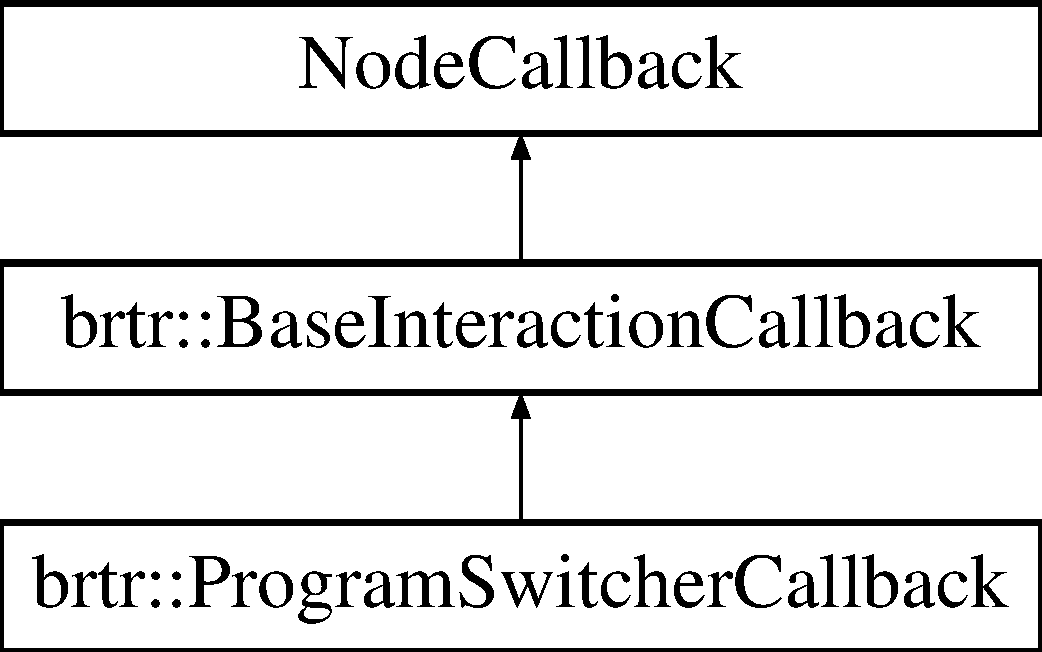
\includegraphics[height=3.000000cm]{classbrtr_1_1_program_switcher_callback}
\end{center}
\end{figure}
\subsection*{Public Member Functions}
\begin{DoxyCompactItemize}
\item 
\hyperlink{classbrtr_1_1_program_switcher_callback_a36a59e70c5db59a00f2d7fd7fbf9e505}{Program\+Switcher\+Callback} (osg\+::\+Node $\ast$postprocess\+Cam, osg\+::\+Camera $\ast$hud\+Cam, int width, int height, std\+::vector$<$ osg\+::ref\+\_\+ptr$<$ osg\+::\+Program $>$$>$ programs)
\begin{DoxyCompactList}\small\item\em Constructor. \end{DoxyCompactList}\item 
virtual void \hyperlink{classbrtr_1_1_program_switcher_callback_a2202619d98a432578c8ed7342b957638}{set\+Text} ()
\begin{DoxyCompactList}\small\item\em sets the text on screen. Subclasses must override to set its own (info)text \end{DoxyCompactList}\end{DoxyCompactItemize}
\subsection*{Protected Member Functions}
\begin{DoxyCompactItemize}
\item 
virtual void \hyperlink{classbrtr_1_1_program_switcher_callback_a06dd3fc2b09d3138e67599d8d56db62a}{interact} (osg\+::\+Node $\ast$, osg\+::\+Node\+Visitor $\ast$)
\begin{DoxyCompactList}\small\item\em each interact sets the next program \end{DoxyCompactList}\end{DoxyCompactItemize}
\subsection*{Private Attributes}
\begin{DoxyCompactItemize}
\item 
std\+::vector$<$ osg\+::ref\+\_\+ptr\\*
$<$ osg\+::\+Program $>$ $>$ \hyperlink{classbrtr_1_1_program_switcher_callback_a9cbcf4d65f6ee468bb20d16b9e795e49}{\+\_\+programs}
\item 
unsigned int \hyperlink{classbrtr_1_1_program_switcher_callback_a06ee6d68fe703e6a88960219b019f1bd}{\+\_\+cur\+Prog}
\end{DoxyCompactItemize}
\subsection*{Additional Inherited Members}


\subsection{Detailed Description}
Callback for switching the postprocess programs. 

Every click the next program in the vector is choosen postprocess\+Cam is the node which stateset holds the programs \begin{DoxyAuthor}{Author}
Gleb Ostrowski 
\end{DoxyAuthor}
\begin{DoxyVersion}{Version}
1.\+0 
\end{DoxyVersion}
\begin{DoxyDate}{Date}
2014 
\end{DoxyDate}
\begin{DoxyCopyright}{Copyright}
G\+N\+U Public License. 
\end{DoxyCopyright}


Definition at line \hyperlink{_program_switcher_callback_8h_source_l00017}{17} of file \hyperlink{_program_switcher_callback_8h_source}{Program\+Switcher\+Callback.\+h}.



\subsection{Constructor \& Destructor Documentation}
\hypertarget{classbrtr_1_1_program_switcher_callback_a36a59e70c5db59a00f2d7fd7fbf9e505}{\index{brtr\+::\+Program\+Switcher\+Callback@{brtr\+::\+Program\+Switcher\+Callback}!Program\+Switcher\+Callback@{Program\+Switcher\+Callback}}
\index{Program\+Switcher\+Callback@{Program\+Switcher\+Callback}!brtr\+::\+Program\+Switcher\+Callback@{brtr\+::\+Program\+Switcher\+Callback}}
\subsubsection[{Program\+Switcher\+Callback}]{\setlength{\rightskip}{0pt plus 5cm}brtr\+::\+Program\+Switcher\+Callback\+::\+Program\+Switcher\+Callback (
\begin{DoxyParamCaption}
\item[{osg\+::\+Node $\ast$}]{postprocess\+Cam, }
\item[{osg\+::\+Camera $\ast$}]{hud\+Cam, }
\item[{int}]{width, }
\item[{int}]{height, }
\item[{std\+::vector$<$ osg\+::ref\+\_\+ptr$<$ osg\+::\+Program $>$$>$}]{programs}
\end{DoxyParamCaption}
)}}\label{classbrtr_1_1_program_switcher_callback_a36a59e70c5db59a00f2d7fd7fbf9e505}


Constructor. 


\begin{DoxyParams}{Parameters}
{\em postprocess\+Cam} & node which stateset contains the programs \\
\hline
{\em hud\+Cam} & \\
\hline
{\em width} & screen\+Width \\
\hline
{\em height} & screen\+Height \\
\hline
{\em programs} & vector with post\+Processprograms \\
\hline
\end{DoxyParams}


Definition at line \hyperlink{_program_switcher_callback_8cpp_source_l00008}{8} of file \hyperlink{_program_switcher_callback_8cpp_source}{Program\+Switcher\+Callback.\+cpp}.



\subsection{Member Function Documentation}
\hypertarget{classbrtr_1_1_program_switcher_callback_a06dd3fc2b09d3138e67599d8d56db62a}{\index{brtr\+::\+Program\+Switcher\+Callback@{brtr\+::\+Program\+Switcher\+Callback}!interact@{interact}}
\index{interact@{interact}!brtr\+::\+Program\+Switcher\+Callback@{brtr\+::\+Program\+Switcher\+Callback}}
\subsubsection[{interact}]{\setlength{\rightskip}{0pt plus 5cm}void brtr\+::\+Program\+Switcher\+Callback\+::interact (
\begin{DoxyParamCaption}
\item[{osg\+::\+Node $\ast$}]{, }
\item[{osg\+::\+Node\+Visitor $\ast$}]{}
\end{DoxyParamCaption}
)\hspace{0.3cm}{\ttfamily [protected]}, {\ttfamily [virtual]}}}\label{classbrtr_1_1_program_switcher_callback_a06dd3fc2b09d3138e67599d8d56db62a}


each interact sets the next program 


\begin{DoxyParams}{Parameters}
{\em not} & used \\
\hline
{\em not} & used \\
\hline
\end{DoxyParams}


Implements \hyperlink{classbrtr_1_1_base_interaction_callback_a3ed50c9c1725f932e0b78c90ba24e1ed}{brtr\+::\+Base\+Interaction\+Callback}.



Definition at line \hyperlink{_program_switcher_callback_8cpp_source_l00017}{17} of file \hyperlink{_program_switcher_callback_8cpp_source}{Program\+Switcher\+Callback.\+cpp}.

\hypertarget{classbrtr_1_1_program_switcher_callback_a2202619d98a432578c8ed7342b957638}{\index{brtr\+::\+Program\+Switcher\+Callback@{brtr\+::\+Program\+Switcher\+Callback}!set\+Text@{set\+Text}}
\index{set\+Text@{set\+Text}!brtr\+::\+Program\+Switcher\+Callback@{brtr\+::\+Program\+Switcher\+Callback}}
\subsubsection[{set\+Text}]{\setlength{\rightskip}{0pt plus 5cm}void brtr\+::\+Program\+Switcher\+Callback\+::set\+Text (
\begin{DoxyParamCaption}
{}
\end{DoxyParamCaption}
)\hspace{0.3cm}{\ttfamily [virtual]}}}\label{classbrtr_1_1_program_switcher_callback_a2202619d98a432578c8ed7342b957638}


sets the text on screen. Subclasses must override to set its own (info)text 



Implements \hyperlink{classbrtr_1_1_base_interaction_callback_a0fe57e329f044e21d49041c861435ad8}{brtr\+::\+Base\+Interaction\+Callback}.



Definition at line \hyperlink{_program_switcher_callback_8cpp_source_l00013}{13} of file \hyperlink{_program_switcher_callback_8cpp_source}{Program\+Switcher\+Callback.\+cpp}.



\subsection{Member Data Documentation}
\hypertarget{classbrtr_1_1_program_switcher_callback_a06ee6d68fe703e6a88960219b019f1bd}{\index{brtr\+::\+Program\+Switcher\+Callback@{brtr\+::\+Program\+Switcher\+Callback}!\+\_\+cur\+Prog@{\+\_\+cur\+Prog}}
\index{\+\_\+cur\+Prog@{\+\_\+cur\+Prog}!brtr\+::\+Program\+Switcher\+Callback@{brtr\+::\+Program\+Switcher\+Callback}}
\subsubsection[{\+\_\+cur\+Prog}]{\setlength{\rightskip}{0pt plus 5cm}unsigned int brtr\+::\+Program\+Switcher\+Callback\+::\+\_\+cur\+Prog\hspace{0.3cm}{\ttfamily [private]}}}\label{classbrtr_1_1_program_switcher_callback_a06ee6d68fe703e6a88960219b019f1bd}


Definition at line \hyperlink{_program_switcher_callback_8h_source_l00041}{41} of file \hyperlink{_program_switcher_callback_8h_source}{Program\+Switcher\+Callback.\+h}.

\hypertarget{classbrtr_1_1_program_switcher_callback_a9cbcf4d65f6ee468bb20d16b9e795e49}{\index{brtr\+::\+Program\+Switcher\+Callback@{brtr\+::\+Program\+Switcher\+Callback}!\+\_\+programs@{\+\_\+programs}}
\index{\+\_\+programs@{\+\_\+programs}!brtr\+::\+Program\+Switcher\+Callback@{brtr\+::\+Program\+Switcher\+Callback}}
\subsubsection[{\+\_\+programs}]{\setlength{\rightskip}{0pt plus 5cm}std\+::vector$<$osg\+::ref\+\_\+ptr$<$osg\+::\+Program$>$ $>$ brtr\+::\+Program\+Switcher\+Callback\+::\+\_\+programs\hspace{0.3cm}{\ttfamily [private]}}}\label{classbrtr_1_1_program_switcher_callback_a9cbcf4d65f6ee468bb20d16b9e795e49}


Definition at line \hyperlink{_program_switcher_callback_8h_source_l00040}{40} of file \hyperlink{_program_switcher_callback_8h_source}{Program\+Switcher\+Callback.\+h}.



The documentation for this class was generated from the following files\+:\begin{DoxyCompactItemize}
\item 
header/\hyperlink{_program_switcher_callback_8h}{Program\+Switcher\+Callback.\+h}\item 
Callbacks/\hyperlink{_program_switcher_callback_8cpp}{Program\+Switcher\+Callback.\+cpp}\end{DoxyCompactItemize}

\hypertarget{structbrtr_1_1_rendering_pipeline}{\section{brtr\+:\+:Rendering\+Pipeline Struct Reference}
\label{structbrtr_1_1_rendering_pipeline}\index{brtr\+::\+Rendering\+Pipeline@{brtr\+::\+Rendering\+Pipeline}}
}


struct holding the camera for the multi-\/rendering passes. Also holds the program vector for the post process pass. pass0\+Color, pass0depth, pass\+Post\+Process, program array, count program\+Array The program vector is used by the \hyperlink{classbrtr_1_1_key_handler}{Key\+Handler} and the Interaction\+Items for changing the postprocess programs  




{\ttfamily \#include $<$Util\+Functions.\+h$>$}

\subsection*{Public Attributes}
\begin{DoxyCompactItemize}
\item 
osg\+::ref\+\_\+ptr$<$ osg\+::\+Camera $>$ \hyperlink{structbrtr_1_1_rendering_pipeline_ae945030321a6b44f00266954c8c50bf3}{pass\+\_\+0\+\_\+color}
\begin{DoxyCompactList}\small\item\em Camera for the first pass, renders the Color\+Buffer to Texture. \end{DoxyCompactList}\item 
osg\+::ref\+\_\+ptr$<$ osg\+::\+Camera $>$ \hyperlink{structbrtr_1_1_rendering_pipeline_a18752632c1b557d283e523ebbc0443a0}{pass\+\_\+0\+\_\+depth}
\begin{DoxyCompactList}\small\item\em Camera for the first pass, renders the Depth\+Buffer to Texture. \end{DoxyCompactList}\item 
osg\+::ref\+\_\+ptr$<$ osg\+::\+Camera $>$ \hyperlink{structbrtr_1_1_rendering_pipeline_aea2228e41f1e5c6db5d616c05ecc27fd}{pass\+\_\+\+Post\+Process}
\begin{DoxyCompactList}\small\item\em Post\+Process Camera, uses the texture from the first pass to create various effects. \end{DoxyCompactList}\item 
std\+::vector$<$ osg\+::ref\+\_\+ptr\\*
$<$ osg\+::\+Program $>$ $>$ \hyperlink{structbrtr_1_1_rendering_pipeline_afe773fb98986d39ef23a4edf3634af10}{programs}
\begin{DoxyCompactList}\small\item\em vector with the avaible postprocess programs \end{DoxyCompactList}\end{DoxyCompactItemize}


\subsection{Detailed Description}
struct holding the camera for the multi-\/rendering passes. Also holds the program vector for the post process pass. pass0\+Color, pass0depth, pass\+Post\+Process, program array, count program\+Array The program vector is used by the \hyperlink{classbrtr_1_1_key_handler}{Key\+Handler} and the Interaction\+Items for changing the postprocess programs 

Definition at line \hyperlink{_util_functions_8h_source_l00056}{56} of file \hyperlink{_util_functions_8h_source}{Util\+Functions.\+h}.



\subsection{Member Data Documentation}
\hypertarget{structbrtr_1_1_rendering_pipeline_ae945030321a6b44f00266954c8c50bf3}{\index{brtr\+::\+Rendering\+Pipeline@{brtr\+::\+Rendering\+Pipeline}!pass\+\_\+0\+\_\+color@{pass\+\_\+0\+\_\+color}}
\index{pass\+\_\+0\+\_\+color@{pass\+\_\+0\+\_\+color}!brtr\+::\+Rendering\+Pipeline@{brtr\+::\+Rendering\+Pipeline}}
\subsubsection[{pass\+\_\+0\+\_\+color}]{\setlength{\rightskip}{0pt plus 5cm}osg\+::ref\+\_\+ptr$<$osg\+::\+Camera$>$ brtr\+::\+Rendering\+Pipeline\+::pass\+\_\+0\+\_\+color}}\label{structbrtr_1_1_rendering_pipeline_ae945030321a6b44f00266954c8c50bf3}


Camera for the first pass, renders the Color\+Buffer to Texture. 



Definition at line \hyperlink{_util_functions_8h_source_l00057}{57} of file \hyperlink{_util_functions_8h_source}{Util\+Functions.\+h}.

\hypertarget{structbrtr_1_1_rendering_pipeline_a18752632c1b557d283e523ebbc0443a0}{\index{brtr\+::\+Rendering\+Pipeline@{brtr\+::\+Rendering\+Pipeline}!pass\+\_\+0\+\_\+depth@{pass\+\_\+0\+\_\+depth}}
\index{pass\+\_\+0\+\_\+depth@{pass\+\_\+0\+\_\+depth}!brtr\+::\+Rendering\+Pipeline@{brtr\+::\+Rendering\+Pipeline}}
\subsubsection[{pass\+\_\+0\+\_\+depth}]{\setlength{\rightskip}{0pt plus 5cm}osg\+::ref\+\_\+ptr$<$osg\+::\+Camera$>$ brtr\+::\+Rendering\+Pipeline\+::pass\+\_\+0\+\_\+depth}}\label{structbrtr_1_1_rendering_pipeline_a18752632c1b557d283e523ebbc0443a0}


Camera for the first pass, renders the Depth\+Buffer to Texture. 



Definition at line \hyperlink{_util_functions_8h_source_l00058}{58} of file \hyperlink{_util_functions_8h_source}{Util\+Functions.\+h}.

\hypertarget{structbrtr_1_1_rendering_pipeline_aea2228e41f1e5c6db5d616c05ecc27fd}{\index{brtr\+::\+Rendering\+Pipeline@{brtr\+::\+Rendering\+Pipeline}!pass\+\_\+\+Post\+Process@{pass\+\_\+\+Post\+Process}}
\index{pass\+\_\+\+Post\+Process@{pass\+\_\+\+Post\+Process}!brtr\+::\+Rendering\+Pipeline@{brtr\+::\+Rendering\+Pipeline}}
\subsubsection[{pass\+\_\+\+Post\+Process}]{\setlength{\rightskip}{0pt plus 5cm}osg\+::ref\+\_\+ptr$<$osg\+::\+Camera$>$ brtr\+::\+Rendering\+Pipeline\+::pass\+\_\+\+Post\+Process}}\label{structbrtr_1_1_rendering_pipeline_aea2228e41f1e5c6db5d616c05ecc27fd}


Post\+Process Camera, uses the texture from the first pass to create various effects. 



Definition at line \hyperlink{_util_functions_8h_source_l00059}{59} of file \hyperlink{_util_functions_8h_source}{Util\+Functions.\+h}.

\hypertarget{structbrtr_1_1_rendering_pipeline_afe773fb98986d39ef23a4edf3634af10}{\index{brtr\+::\+Rendering\+Pipeline@{brtr\+::\+Rendering\+Pipeline}!programs@{programs}}
\index{programs@{programs}!brtr\+::\+Rendering\+Pipeline@{brtr\+::\+Rendering\+Pipeline}}
\subsubsection[{programs}]{\setlength{\rightskip}{0pt plus 5cm}std\+::vector$<$osg\+::ref\+\_\+ptr$<$osg\+::\+Program$>$ $>$ brtr\+::\+Rendering\+Pipeline\+::programs}}\label{structbrtr_1_1_rendering_pipeline_afe773fb98986d39ef23a4edf3634af10}


vector with the avaible postprocess programs 



Definition at line \hyperlink{_util_functions_8h_source_l00060}{60} of file \hyperlink{_util_functions_8h_source}{Util\+Functions.\+h}.



The documentation for this struct was generated from the following file\+:\begin{DoxyCompactItemize}
\item 
header/\hyperlink{_util_functions_8h}{Util\+Functions.\+h}\end{DoxyCompactItemize}

\hypertarget{classbrtr_1_1_toon_tex_switcher_callback}{\section{brtr\+:\+:Toon\+Tex\+Switcher\+Callback Class Reference}
\label{classbrtr_1_1_toon_tex_switcher_callback}\index{brtr\+::\+Toon\+Tex\+Switcher\+Callback@{brtr\+::\+Toon\+Tex\+Switcher\+Callback}}
}


Callback for switching the Toon\+Textures.  




{\ttfamily \#include $<$Toon\+Tex\+Switcher\+Callback.\+h$>$}

Inheritance diagram for brtr\+:\+:Toon\+Tex\+Switcher\+Callback\+:\begin{figure}[H]
\begin{center}
\leavevmode
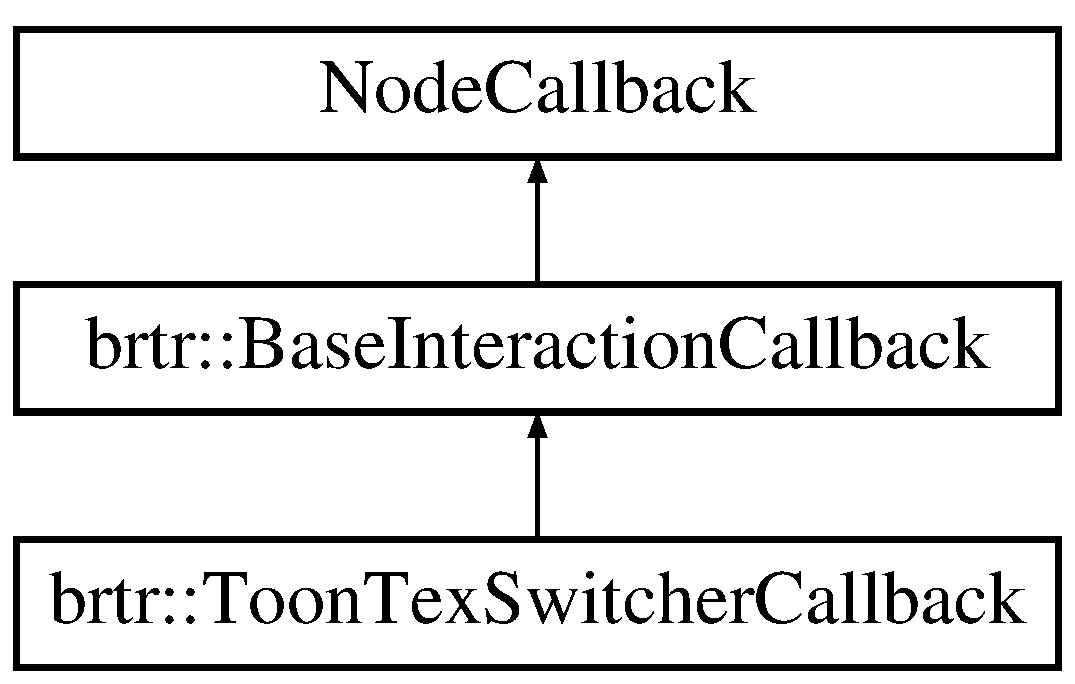
\includegraphics[height=3.000000cm]{classbrtr_1_1_toon_tex_switcher_callback}
\end{center}
\end{figure}
\subsection*{Public Member Functions}
\begin{DoxyCompactItemize}
\item 
\hyperlink{classbrtr_1_1_toon_tex_switcher_callback_ae117afe5056c885a625a850e1d0fbae7}{Toon\+Tex\+Switcher\+Callback} (osg\+::\+Node $\ast$scenedata, osg\+::\+Camera $\ast$hud\+Cam, int width, int height, std\+::vector$<$ osg\+::ref\+\_\+ptr$<$ osg\+::\+Texture2\+D $>$$>$ toon\+Texs)
\begin{DoxyCompactList}\small\item\em Constructor. \end{DoxyCompactList}\item 
virtual void \hyperlink{classbrtr_1_1_toon_tex_switcher_callback_aad13301231829b5c28f14910d4d44355}{set\+Text} ()
\begin{DoxyCompactList}\small\item\em sets the text on screen. Subclasses must override to set its own (info)text \end{DoxyCompactList}\end{DoxyCompactItemize}
\subsection*{Protected Member Functions}
\begin{DoxyCompactItemize}
\item 
virtual void \hyperlink{classbrtr_1_1_toon_tex_switcher_callback_a97047bc2817ddfecc2c1531d22e289fd}{interact} (osg\+::\+Node $\ast$node, osg\+::\+Node\+Visitor $\ast$)
\begin{DoxyCompactList}\small\item\em each interact sets the next texture \end{DoxyCompactList}\end{DoxyCompactItemize}
\subsection*{Private Attributes}
\begin{DoxyCompactItemize}
\item 
int \hyperlink{classbrtr_1_1_toon_tex_switcher_callback_a58030dcd246f0f2c168965ca087cfa17}{\+\_\+cur\+Tex}
\item 
std\+::vector$<$ osg\+::ref\+\_\+ptr\\*
$<$ osg\+::\+Texture2\+D $>$ $>$ \hyperlink{classbrtr_1_1_toon_tex_switcher_callback_a96cbd2a83f9ed21efde9d086c34e6d5e}{\+\_\+toon\+Texs}
\end{DoxyCompactItemize}
\subsection*{Additional Inherited Members}


\subsection{Detailed Description}
Callback for switching the Toon\+Textures. 

Every click the next texture in the vector is choosen scenedata is the node which stateset holds the textures \begin{DoxyAuthor}{Author}
Gleb Ostrowski 
\end{DoxyAuthor}
\begin{DoxyVersion}{Version}
1.\+0 
\end{DoxyVersion}
\begin{DoxyDate}{Date}
2014 
\end{DoxyDate}
\begin{DoxyCopyright}{Copyright}
G\+N\+U Public License. 
\end{DoxyCopyright}


Definition at line \hyperlink{_toon_tex_switcher_callback_8h_source_l00017}{17} of file \hyperlink{_toon_tex_switcher_callback_8h_source}{Toon\+Tex\+Switcher\+Callback.\+h}.



\subsection{Constructor \& Destructor Documentation}
\hypertarget{classbrtr_1_1_toon_tex_switcher_callback_ae117afe5056c885a625a850e1d0fbae7}{\index{brtr\+::\+Toon\+Tex\+Switcher\+Callback@{brtr\+::\+Toon\+Tex\+Switcher\+Callback}!Toon\+Tex\+Switcher\+Callback@{Toon\+Tex\+Switcher\+Callback}}
\index{Toon\+Tex\+Switcher\+Callback@{Toon\+Tex\+Switcher\+Callback}!brtr\+::\+Toon\+Tex\+Switcher\+Callback@{brtr\+::\+Toon\+Tex\+Switcher\+Callback}}
\subsubsection[{Toon\+Tex\+Switcher\+Callback}]{\setlength{\rightskip}{0pt plus 5cm}brtr\+::\+Toon\+Tex\+Switcher\+Callback\+::\+Toon\+Tex\+Switcher\+Callback (
\begin{DoxyParamCaption}
\item[{osg\+::\+Node $\ast$}]{scenedata, }
\item[{osg\+::\+Camera $\ast$}]{hud\+Cam, }
\item[{int}]{width, }
\item[{int}]{height, }
\item[{std\+::vector$<$ osg\+::ref\+\_\+ptr$<$ osg\+::\+Texture2\+D $>$$>$}]{toon\+Texs}
\end{DoxyParamCaption}
)}}\label{classbrtr_1_1_toon_tex_switcher_callback_ae117afe5056c885a625a850e1d0fbae7}


Constructor. 


\begin{DoxyParams}{Parameters}
{\em scenedata} & node which stateset contains the Toon\+Textures \\
\hline
{\em hud\+Cam} & \\
\hline
{\em width} & screen\+Width \\
\hline
{\em height} & screen\+Height \\
\hline
{\em toon\+Texs} & vector with Toon\+Textures \\
\hline
\end{DoxyParams}


Definition at line \hyperlink{_toon_tex_switcher_callback_8cpp_source_l00009}{9} of file \hyperlink{_toon_tex_switcher_callback_8cpp_source}{Toon\+Tex\+Switcher\+Callback.\+cpp}.



\subsection{Member Function Documentation}
\hypertarget{classbrtr_1_1_toon_tex_switcher_callback_a97047bc2817ddfecc2c1531d22e289fd}{\index{brtr\+::\+Toon\+Tex\+Switcher\+Callback@{brtr\+::\+Toon\+Tex\+Switcher\+Callback}!interact@{interact}}
\index{interact@{interact}!brtr\+::\+Toon\+Tex\+Switcher\+Callback@{brtr\+::\+Toon\+Tex\+Switcher\+Callback}}
\subsubsection[{interact}]{\setlength{\rightskip}{0pt plus 5cm}void brtr\+::\+Toon\+Tex\+Switcher\+Callback\+::interact (
\begin{DoxyParamCaption}
\item[{osg\+::\+Node $\ast$}]{node, }
\item[{osg\+::\+Node\+Visitor $\ast$}]{}
\end{DoxyParamCaption}
)\hspace{0.3cm}{\ttfamily [protected]}, {\ttfamily [virtual]}}}\label{classbrtr_1_1_toon_tex_switcher_callback_a97047bc2817ddfecc2c1531d22e289fd}


each interact sets the next texture 


\begin{DoxyParams}{Parameters}
{\em not} & used \\
\hline
{\em not} & used \\
\hline
\end{DoxyParams}


Implements \hyperlink{classbrtr_1_1_base_interaction_callback_a3ed50c9c1725f932e0b78c90ba24e1ed}{brtr\+::\+Base\+Interaction\+Callback}.



Definition at line \hyperlink{_toon_tex_switcher_callback_8cpp_source_l00018}{18} of file \hyperlink{_toon_tex_switcher_callback_8cpp_source}{Toon\+Tex\+Switcher\+Callback.\+cpp}.

\hypertarget{classbrtr_1_1_toon_tex_switcher_callback_aad13301231829b5c28f14910d4d44355}{\index{brtr\+::\+Toon\+Tex\+Switcher\+Callback@{brtr\+::\+Toon\+Tex\+Switcher\+Callback}!set\+Text@{set\+Text}}
\index{set\+Text@{set\+Text}!brtr\+::\+Toon\+Tex\+Switcher\+Callback@{brtr\+::\+Toon\+Tex\+Switcher\+Callback}}
\subsubsection[{set\+Text}]{\setlength{\rightskip}{0pt plus 5cm}void brtr\+::\+Toon\+Tex\+Switcher\+Callback\+::set\+Text (
\begin{DoxyParamCaption}
{}
\end{DoxyParamCaption}
)\hspace{0.3cm}{\ttfamily [virtual]}}}\label{classbrtr_1_1_toon_tex_switcher_callback_aad13301231829b5c28f14910d4d44355}


sets the text on screen. Subclasses must override to set its own (info)text 



Implements \hyperlink{classbrtr_1_1_base_interaction_callback_a0fe57e329f044e21d49041c861435ad8}{brtr\+::\+Base\+Interaction\+Callback}.



Definition at line \hyperlink{_toon_tex_switcher_callback_8cpp_source_l00014}{14} of file \hyperlink{_toon_tex_switcher_callback_8cpp_source}{Toon\+Tex\+Switcher\+Callback.\+cpp}.



\subsection{Member Data Documentation}
\hypertarget{classbrtr_1_1_toon_tex_switcher_callback_a58030dcd246f0f2c168965ca087cfa17}{\index{brtr\+::\+Toon\+Tex\+Switcher\+Callback@{brtr\+::\+Toon\+Tex\+Switcher\+Callback}!\+\_\+cur\+Tex@{\+\_\+cur\+Tex}}
\index{\+\_\+cur\+Tex@{\+\_\+cur\+Tex}!brtr\+::\+Toon\+Tex\+Switcher\+Callback@{brtr\+::\+Toon\+Tex\+Switcher\+Callback}}
\subsubsection[{\+\_\+cur\+Tex}]{\setlength{\rightskip}{0pt plus 5cm}int brtr\+::\+Toon\+Tex\+Switcher\+Callback\+::\+\_\+cur\+Tex\hspace{0.3cm}{\ttfamily [private]}}}\label{classbrtr_1_1_toon_tex_switcher_callback_a58030dcd246f0f2c168965ca087cfa17}


Definition at line \hyperlink{_toon_tex_switcher_callback_8h_source_l00040}{40} of file \hyperlink{_toon_tex_switcher_callback_8h_source}{Toon\+Tex\+Switcher\+Callback.\+h}.

\hypertarget{classbrtr_1_1_toon_tex_switcher_callback_a96cbd2a83f9ed21efde9d086c34e6d5e}{\index{brtr\+::\+Toon\+Tex\+Switcher\+Callback@{brtr\+::\+Toon\+Tex\+Switcher\+Callback}!\+\_\+toon\+Texs@{\+\_\+toon\+Texs}}
\index{\+\_\+toon\+Texs@{\+\_\+toon\+Texs}!brtr\+::\+Toon\+Tex\+Switcher\+Callback@{brtr\+::\+Toon\+Tex\+Switcher\+Callback}}
\subsubsection[{\+\_\+toon\+Texs}]{\setlength{\rightskip}{0pt plus 5cm}std\+::vector$<$osg\+::ref\+\_\+ptr$<$osg\+::\+Texture2\+D$>$ $>$ brtr\+::\+Toon\+Tex\+Switcher\+Callback\+::\+\_\+toon\+Texs\hspace{0.3cm}{\ttfamily [private]}}}\label{classbrtr_1_1_toon_tex_switcher_callback_a96cbd2a83f9ed21efde9d086c34e6d5e}


Definition at line \hyperlink{_toon_tex_switcher_callback_8h_source_l00041}{41} of file \hyperlink{_toon_tex_switcher_callback_8h_source}{Toon\+Tex\+Switcher\+Callback.\+h}.



The documentation for this class was generated from the following files\+:\begin{DoxyCompactItemize}
\item 
header/\hyperlink{_toon_tex_switcher_callback_8h}{Toon\+Tex\+Switcher\+Callback.\+h}\item 
Callbacks/\hyperlink{_toon_tex_switcher_callback_8cpp}{Toon\+Tex\+Switcher\+Callback.\+cpp}\end{DoxyCompactItemize}

\hypertarget{classbrtr_1_1_train_switcher_callback}{\section{brtr\+:\+:Train\+Switcher\+Callback Class Reference}
\label{classbrtr_1_1_train_switcher_callback}\index{brtr\+::\+Train\+Switcher\+Callback@{brtr\+::\+Train\+Switcher\+Callback}}
}


Callback for switching the \char`\"{}trains\char`\"{}.  




{\ttfamily \#include $<$Train\+Switcher\+Callback.\+h$>$}

Inheritance diagram for brtr\+:\+:Train\+Switcher\+Callback\+:\begin{figure}[H]
\begin{center}
\leavevmode
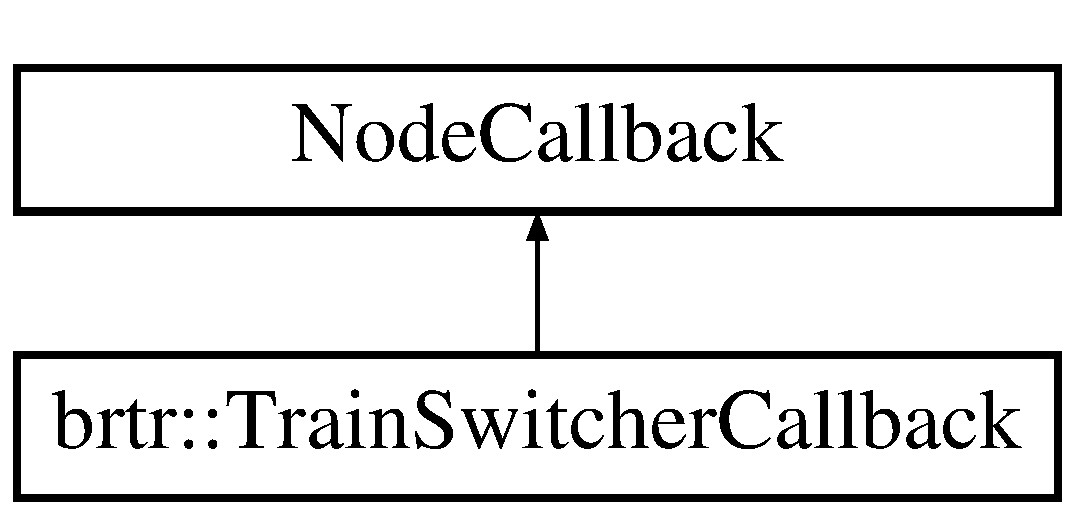
\includegraphics[height=2.000000cm]{classbrtr_1_1_train_switcher_callback}
\end{center}
\end{figure}
\subsection*{Public Member Functions}
\begin{DoxyCompactItemize}
\item 
\hyperlink{classbrtr_1_1_train_switcher_callback_a54ad53b07976bf34af2a0e6061088f3c}{Train\+Switcher\+Callback} ()
\item 
virtual void \hyperlink{classbrtr_1_1_train_switcher_callback_a5a8182c650febc07a8443f6a35c32087}{operator()} (osg\+::\+Node $\ast$node, osg\+::\+Node\+Visitor $\ast$nv)
\end{DoxyCompactItemize}
\subsection*{Private Attributes}
\begin{DoxyCompactItemize}
\item 
int \hyperlink{classbrtr_1_1_train_switcher_callback_ac87e64555ad379814a93220447c49257}{\+\_\+cur\+Active\+Train}
\item 
int \hyperlink{classbrtr_1_1_train_switcher_callback_a1d2fbe75d19ca03cba449cdf4277f0eb}{\+\_\+delta\+Time}
\end{DoxyCompactItemize}


\subsection{Detailed Description}
Callback for switching the \char`\"{}trains\char`\"{}. 

every $\sim$36 secs the \char`\"{}train\char`\"{} on the rails switched \begin{DoxyAuthor}{Author}
Gleb Ostrowski 
\end{DoxyAuthor}
\begin{DoxyVersion}{Version}
1.\+0 
\end{DoxyVersion}
\begin{DoxyDate}{Date}
2014 
\end{DoxyDate}
\begin{DoxyPrecond}{Precondition}
needs to be attached to a switch node 
\end{DoxyPrecond}
\begin{DoxyCopyright}{Copyright}
G\+N\+U Public License. 
\end{DoxyCopyright}


Definition at line \hyperlink{_train_switcher_callback_8h_source_l00015}{15} of file \hyperlink{_train_switcher_callback_8h_source}{Train\+Switcher\+Callback.\+h}.



\subsection{Constructor \& Destructor Documentation}
\hypertarget{classbrtr_1_1_train_switcher_callback_a54ad53b07976bf34af2a0e6061088f3c}{\index{brtr\+::\+Train\+Switcher\+Callback@{brtr\+::\+Train\+Switcher\+Callback}!Train\+Switcher\+Callback@{Train\+Switcher\+Callback}}
\index{Train\+Switcher\+Callback@{Train\+Switcher\+Callback}!brtr\+::\+Train\+Switcher\+Callback@{brtr\+::\+Train\+Switcher\+Callback}}
\subsubsection[{Train\+Switcher\+Callback}]{\setlength{\rightskip}{0pt plus 5cm}brtr\+::\+Train\+Switcher\+Callback\+::\+Train\+Switcher\+Callback (
\begin{DoxyParamCaption}
{}
\end{DoxyParamCaption}
)}}\label{classbrtr_1_1_train_switcher_callback_a54ad53b07976bf34af2a0e6061088f3c}


Definition at line \hyperlink{_train_switcher_callback_8cpp_source_l00004}{4} of file \hyperlink{_train_switcher_callback_8cpp_source}{Train\+Switcher\+Callback.\+cpp}.



\subsection{Member Function Documentation}
\hypertarget{classbrtr_1_1_train_switcher_callback_a5a8182c650febc07a8443f6a35c32087}{\index{brtr\+::\+Train\+Switcher\+Callback@{brtr\+::\+Train\+Switcher\+Callback}!operator()@{operator()}}
\index{operator()@{operator()}!brtr\+::\+Train\+Switcher\+Callback@{brtr\+::\+Train\+Switcher\+Callback}}
\subsubsection[{operator()}]{\setlength{\rightskip}{0pt plus 5cm}void brtr\+::\+Train\+Switcher\+Callback\+::operator() (
\begin{DoxyParamCaption}
\item[{osg\+::\+Node $\ast$}]{node, }
\item[{osg\+::\+Node\+Visitor $\ast$}]{nv}
\end{DoxyParamCaption}
)\hspace{0.3cm}{\ttfamily [virtual]}}}\label{classbrtr_1_1_train_switcher_callback_a5a8182c650febc07a8443f6a35c32087}


Definition at line \hyperlink{_train_switcher_callback_8cpp_source_l00008}{8} of file \hyperlink{_train_switcher_callback_8cpp_source}{Train\+Switcher\+Callback.\+cpp}.



\subsection{Member Data Documentation}
\hypertarget{classbrtr_1_1_train_switcher_callback_ac87e64555ad379814a93220447c49257}{\index{brtr\+::\+Train\+Switcher\+Callback@{brtr\+::\+Train\+Switcher\+Callback}!\+\_\+cur\+Active\+Train@{\+\_\+cur\+Active\+Train}}
\index{\+\_\+cur\+Active\+Train@{\+\_\+cur\+Active\+Train}!brtr\+::\+Train\+Switcher\+Callback@{brtr\+::\+Train\+Switcher\+Callback}}
\subsubsection[{\+\_\+cur\+Active\+Train}]{\setlength{\rightskip}{0pt plus 5cm}int brtr\+::\+Train\+Switcher\+Callback\+::\+\_\+cur\+Active\+Train\hspace{0.3cm}{\ttfamily [private]}}}\label{classbrtr_1_1_train_switcher_callback_ac87e64555ad379814a93220447c49257}


Definition at line \hyperlink{_train_switcher_callback_8h_source_l00021}{21} of file \hyperlink{_train_switcher_callback_8h_source}{Train\+Switcher\+Callback.\+h}.

\hypertarget{classbrtr_1_1_train_switcher_callback_a1d2fbe75d19ca03cba449cdf4277f0eb}{\index{brtr\+::\+Train\+Switcher\+Callback@{brtr\+::\+Train\+Switcher\+Callback}!\+\_\+delta\+Time@{\+\_\+delta\+Time}}
\index{\+\_\+delta\+Time@{\+\_\+delta\+Time}!brtr\+::\+Train\+Switcher\+Callback@{brtr\+::\+Train\+Switcher\+Callback}}
\subsubsection[{\+\_\+delta\+Time}]{\setlength{\rightskip}{0pt plus 5cm}int brtr\+::\+Train\+Switcher\+Callback\+::\+\_\+delta\+Time\hspace{0.3cm}{\ttfamily [private]}}}\label{classbrtr_1_1_train_switcher_callback_a1d2fbe75d19ca03cba449cdf4277f0eb}


Definition at line \hyperlink{_train_switcher_callback_8h_source_l00022}{22} of file \hyperlink{_train_switcher_callback_8h_source}{Train\+Switcher\+Callback.\+h}.



The documentation for this class was generated from the following files\+:\begin{DoxyCompactItemize}
\item 
header/\hyperlink{_train_switcher_callback_8h}{Train\+Switcher\+Callback.\+h}\item 
Callbacks/\hyperlink{_train_switcher_callback_8cpp}{Train\+Switcher\+Callback.\+cpp}\end{DoxyCompactItemize}

\hypertarget{classbrtr_1_1_weapon_h_u_d}{\section{brtr\+:\+:Weapon\+H\+U\+D Class Reference}
\label{classbrtr_1_1_weapon_h_u_d}\index{brtr\+::\+Weapon\+H\+U\+D@{brtr\+::\+Weapon\+H\+U\+D}}
}


\hyperlink{classbrtr_1_1_weapon_h_u_d}{Weapon\+H\+U\+D} class, provides the functions to add a H\+U\+D camera to the scene.  




{\ttfamily \#include $<$Weapon\+H\+U\+D.\+h$>$}

Inheritance diagram for brtr\+:\+:Weapon\+H\+U\+D\+:\begin{figure}[H]
\begin{center}
\leavevmode
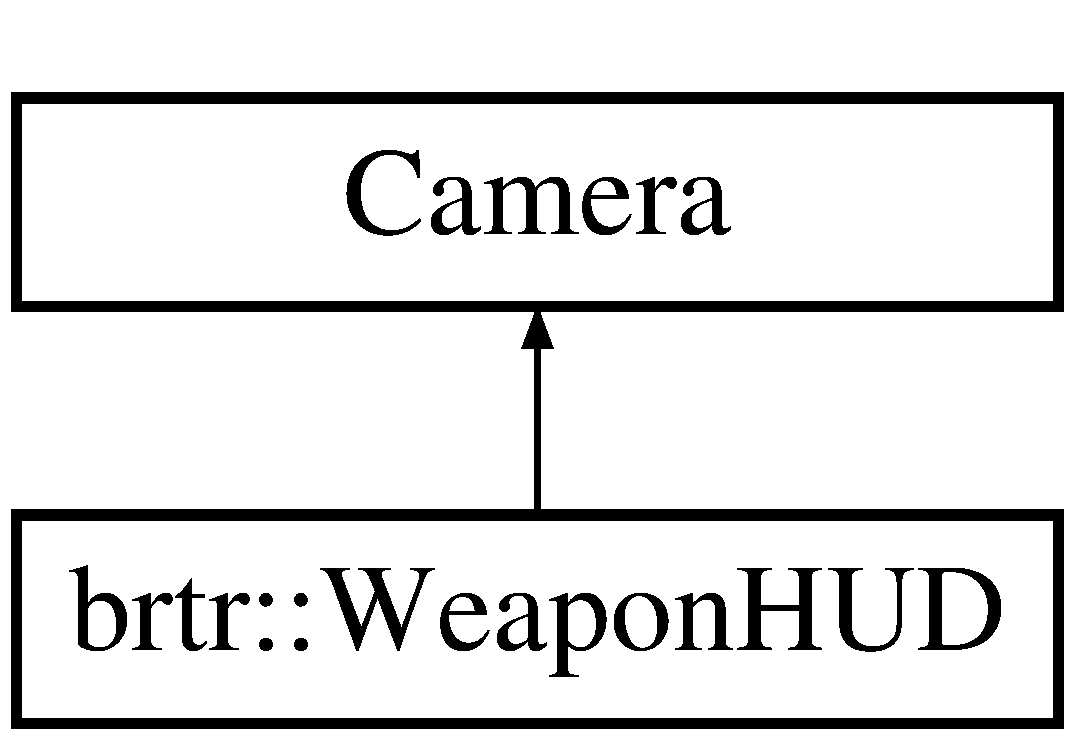
\includegraphics[height=2.000000cm]{classbrtr_1_1_weapon_h_u_d}
\end{center}
\end{figure}
\subsection*{Classes}
\begin{DoxyCompactItemize}
\item 
class \hyperlink{classbrtr_1_1_weapon_h_u_d_1_1_weapon_switch_handler}{Weapon\+Switch\+Handler}
\begin{DoxyCompactList}\small\item\em Event\+Handler for Weapon\+Switching. \end{DoxyCompactList}\end{DoxyCompactItemize}
\subsection*{Public Member Functions}
\begin{DoxyCompactItemize}
\item 
\hyperlink{classbrtr_1_1_weapon_h_u_d_a8bc53d9bc7df80c28e2d9eeeed113281}{Weapon\+H\+U\+D} ()
\item 
\hyperlink{classbrtr_1_1_weapon_h_u_d_a79723105b944c088928741a620551d8d}{Weapon\+H\+U\+D} (const \hyperlink{classbrtr_1_1_weapon_h_u_d}{Weapon\+H\+U\+D} \&, const Copy\+Op \&copyop=Copy\+Op\+::\+S\+H\+A\+L\+L\+O\+W\+\_\+\+C\+O\+P\+Y)
\item 
ref\+\_\+ptr$<$ \hyperlink{classbrtr_1_1_weapon_h_u_d_1_1_weapon_switch_handler}{Weapon\+Switch\+Handler} $>$ \hyperlink{classbrtr_1_1_weapon_h_u_d_a6a9a434ff3aa3861caf030763772ac74}{get\+Weapon\+Handler} ()
\item 
void \hyperlink{classbrtr_1_1_weapon_h_u_d_ab8ccf2821f698af567b7ce40eb6840d8}{add\+Portal\+Gun} ()
\begin{DoxyCompactList}\small\item\em a portal gun is added to the weapon switch \end{DoxyCompactList}\item 
\hyperlink{classbrtr_1_1_weapon_h_u_d_aaaa6c5e92034b7efb6194032f6ffca0f}{$\sim$\+Weapon\+H\+U\+D} ()
\end{DoxyCompactItemize}
\subsection*{Private Member Functions}
\begin{DoxyCompactItemize}
\item 
void \hyperlink{classbrtr_1_1_weapon_h_u_d_a86191d6e9041afc84575e77576464da9}{create\+Weapon\+H\+U\+D} ()
\begin{DoxyCompactList}\small\item\em creates a weapon hud with the default weapon crowbar \end{DoxyCompactList}\end{DoxyCompactItemize}
\subsection*{Private Attributes}
\begin{DoxyCompactItemize}
\item 
ref\+\_\+ptr$<$ Switch $>$ \hyperlink{classbrtr_1_1_weapon_h_u_d_a32d5e498c15faa87f3bcfa83ca6c5b0e}{\+\_\+switcher}
\item 
ref\+\_\+ptr$<$ \hyperlink{classbrtr_1_1_weapon_h_u_d_1_1_weapon_switch_handler}{Weapon\+Switch\+Handler} $>$ \hyperlink{classbrtr_1_1_weapon_h_u_d_a4ebf9d9e600e3a6b9f5d8601c084ee51}{\+\_\+handler}
\end{DoxyCompactItemize}


\subsection{Detailed Description}
\hyperlink{classbrtr_1_1_weapon_h_u_d}{Weapon\+H\+U\+D} class, provides the functions to add a H\+U\+D camera to the scene. 

Use the mouse wheel to shift between weapons after picking up a second one \begin{DoxyAuthor}{Author}
Jonathan Spielvogel 
\end{DoxyAuthor}
\begin{DoxyVersion}{Version}
1.\+0 
\end{DoxyVersion}
\begin{DoxyDate}{Date}
2014 
\end{DoxyDate}
\begin{DoxyPrecond}{Precondition}
create a root node and attach the scene to it, then add the H\+U\+D to root 
\end{DoxyPrecond}
\begin{DoxyCopyright}{Copyright}
G\+N\+U Public License. 
\end{DoxyCopyright}


Definition at line \hyperlink{_weapon_h_u_d_8h_source_l00023}{23} of file \hyperlink{_weapon_h_u_d_8h_source}{Weapon\+H\+U\+D.\+h}.



\subsection{Constructor \& Destructor Documentation}
\hypertarget{classbrtr_1_1_weapon_h_u_d_a8bc53d9bc7df80c28e2d9eeeed113281}{\index{brtr\+::\+Weapon\+H\+U\+D@{brtr\+::\+Weapon\+H\+U\+D}!Weapon\+H\+U\+D@{Weapon\+H\+U\+D}}
\index{Weapon\+H\+U\+D@{Weapon\+H\+U\+D}!brtr\+::\+Weapon\+H\+U\+D@{brtr\+::\+Weapon\+H\+U\+D}}
\subsubsection[{Weapon\+H\+U\+D}]{\setlength{\rightskip}{0pt plus 5cm}brtr\+::\+Weapon\+H\+U\+D\+::\+Weapon\+H\+U\+D (
\begin{DoxyParamCaption}
{}
\end{DoxyParamCaption}
)}}\label{classbrtr_1_1_weapon_h_u_d_a8bc53d9bc7df80c28e2d9eeeed113281}


Definition at line \hyperlink{_weapon_h_u_d_8cpp_source_l00018}{18} of file \hyperlink{_weapon_h_u_d_8cpp_source}{Weapon\+H\+U\+D.\+cpp}.

\hypertarget{classbrtr_1_1_weapon_h_u_d_a79723105b944c088928741a620551d8d}{\index{brtr\+::\+Weapon\+H\+U\+D@{brtr\+::\+Weapon\+H\+U\+D}!Weapon\+H\+U\+D@{Weapon\+H\+U\+D}}
\index{Weapon\+H\+U\+D@{Weapon\+H\+U\+D}!brtr\+::\+Weapon\+H\+U\+D@{brtr\+::\+Weapon\+H\+U\+D}}
\subsubsection[{Weapon\+H\+U\+D}]{\setlength{\rightskip}{0pt plus 5cm}brtr\+::\+Weapon\+H\+U\+D\+::\+Weapon\+H\+U\+D (
\begin{DoxyParamCaption}
\item[{const {\bf Weapon\+H\+U\+D} \&}]{copy, }
\item[{const Copy\+Op \&}]{copyop = {\ttfamily CopyOp\+:\+:SHALLOW\+\_\+COPY}}
\end{DoxyParamCaption}
)}}\label{classbrtr_1_1_weapon_h_u_d_a79723105b944c088928741a620551d8d}


Definition at line \hyperlink{_weapon_h_u_d_8cpp_source_l00011}{11} of file \hyperlink{_weapon_h_u_d_8cpp_source}{Weapon\+H\+U\+D.\+cpp}.

\hypertarget{classbrtr_1_1_weapon_h_u_d_aaaa6c5e92034b7efb6194032f6ffca0f}{\index{brtr\+::\+Weapon\+H\+U\+D@{brtr\+::\+Weapon\+H\+U\+D}!````~Weapon\+H\+U\+D@{$\sim$\+Weapon\+H\+U\+D}}
\index{````~Weapon\+H\+U\+D@{$\sim$\+Weapon\+H\+U\+D}!brtr\+::\+Weapon\+H\+U\+D@{brtr\+::\+Weapon\+H\+U\+D}}
\subsubsection[{$\sim$\+Weapon\+H\+U\+D}]{\setlength{\rightskip}{0pt plus 5cm}brtr\+::\+Weapon\+H\+U\+D\+::$\sim$\+Weapon\+H\+U\+D (
\begin{DoxyParamCaption}
{}
\end{DoxyParamCaption}
)}}\label{classbrtr_1_1_weapon_h_u_d_aaaa6c5e92034b7efb6194032f6ffca0f}


Definition at line \hyperlink{_weapon_h_u_d_8cpp_source_l00065}{65} of file \hyperlink{_weapon_h_u_d_8cpp_source}{Weapon\+H\+U\+D.\+cpp}.



\subsection{Member Function Documentation}
\hypertarget{classbrtr_1_1_weapon_h_u_d_ab8ccf2821f698af567b7ce40eb6840d8}{\index{brtr\+::\+Weapon\+H\+U\+D@{brtr\+::\+Weapon\+H\+U\+D}!add\+Portal\+Gun@{add\+Portal\+Gun}}
\index{add\+Portal\+Gun@{add\+Portal\+Gun}!brtr\+::\+Weapon\+H\+U\+D@{brtr\+::\+Weapon\+H\+U\+D}}
\subsubsection[{add\+Portal\+Gun}]{\setlength{\rightskip}{0pt plus 5cm}void brtr\+::\+Weapon\+H\+U\+D\+::add\+Portal\+Gun (
\begin{DoxyParamCaption}
{}
\end{DoxyParamCaption}
)}}\label{classbrtr_1_1_weapon_h_u_d_ab8ccf2821f698af567b7ce40eb6840d8}


a portal gun is added to the weapon switch 



Definition at line \hyperlink{_weapon_h_u_d_8cpp_source_l00073}{73} of file \hyperlink{_weapon_h_u_d_8cpp_source}{Weapon\+H\+U\+D.\+cpp}.

\hypertarget{classbrtr_1_1_weapon_h_u_d_a86191d6e9041afc84575e77576464da9}{\index{brtr\+::\+Weapon\+H\+U\+D@{brtr\+::\+Weapon\+H\+U\+D}!create\+Weapon\+H\+U\+D@{create\+Weapon\+H\+U\+D}}
\index{create\+Weapon\+H\+U\+D@{create\+Weapon\+H\+U\+D}!brtr\+::\+Weapon\+H\+U\+D@{brtr\+::\+Weapon\+H\+U\+D}}
\subsubsection[{create\+Weapon\+H\+U\+D}]{\setlength{\rightskip}{0pt plus 5cm}void brtr\+::\+Weapon\+H\+U\+D\+::create\+Weapon\+H\+U\+D (
\begin{DoxyParamCaption}
{}
\end{DoxyParamCaption}
)\hspace{0.3cm}{\ttfamily [private]}}}\label{classbrtr_1_1_weapon_h_u_d_a86191d6e9041afc84575e77576464da9}


creates a weapon hud with the default weapon crowbar 



Definition at line \hyperlink{_weapon_h_u_d_8cpp_source_l00022}{22} of file \hyperlink{_weapon_h_u_d_8cpp_source}{Weapon\+H\+U\+D.\+cpp}.

\hypertarget{classbrtr_1_1_weapon_h_u_d_a6a9a434ff3aa3861caf030763772ac74}{\index{brtr\+::\+Weapon\+H\+U\+D@{brtr\+::\+Weapon\+H\+U\+D}!get\+Weapon\+Handler@{get\+Weapon\+Handler}}
\index{get\+Weapon\+Handler@{get\+Weapon\+Handler}!brtr\+::\+Weapon\+H\+U\+D@{brtr\+::\+Weapon\+H\+U\+D}}
\subsubsection[{get\+Weapon\+Handler}]{\setlength{\rightskip}{0pt plus 5cm}ref\+\_\+ptr$<$ {\bf Weapon\+H\+U\+D\+::\+Weapon\+Switch\+Handler} $>$ brtr\+::\+Weapon\+H\+U\+D\+::get\+Weapon\+Handler (
\begin{DoxyParamCaption}
{}
\end{DoxyParamCaption}
)}}\label{classbrtr_1_1_weapon_h_u_d_a6a9a434ff3aa3861caf030763772ac74}


Definition at line \hyperlink{_weapon_h_u_d_8cpp_source_l00069}{69} of file \hyperlink{_weapon_h_u_d_8cpp_source}{Weapon\+H\+U\+D.\+cpp}.



\subsection{Member Data Documentation}
\hypertarget{classbrtr_1_1_weapon_h_u_d_a4ebf9d9e600e3a6b9f5d8601c084ee51}{\index{brtr\+::\+Weapon\+H\+U\+D@{brtr\+::\+Weapon\+H\+U\+D}!\+\_\+handler@{\+\_\+handler}}
\index{\+\_\+handler@{\+\_\+handler}!brtr\+::\+Weapon\+H\+U\+D@{brtr\+::\+Weapon\+H\+U\+D}}
\subsubsection[{\+\_\+handler}]{\setlength{\rightskip}{0pt plus 5cm}ref\+\_\+ptr$<${\bf Weapon\+Switch\+Handler}$>$ brtr\+::\+Weapon\+H\+U\+D\+::\+\_\+handler\hspace{0.3cm}{\ttfamily [private]}}}\label{classbrtr_1_1_weapon_h_u_d_a4ebf9d9e600e3a6b9f5d8601c084ee51}


Definition at line \hyperlink{_weapon_h_u_d_8h_source_l00073}{73} of file \hyperlink{_weapon_h_u_d_8h_source}{Weapon\+H\+U\+D.\+h}.

\hypertarget{classbrtr_1_1_weapon_h_u_d_a32d5e498c15faa87f3bcfa83ca6c5b0e}{\index{brtr\+::\+Weapon\+H\+U\+D@{brtr\+::\+Weapon\+H\+U\+D}!\+\_\+switcher@{\+\_\+switcher}}
\index{\+\_\+switcher@{\+\_\+switcher}!brtr\+::\+Weapon\+H\+U\+D@{brtr\+::\+Weapon\+H\+U\+D}}
\subsubsection[{\+\_\+switcher}]{\setlength{\rightskip}{0pt plus 5cm}ref\+\_\+ptr$<$Switch$>$ brtr\+::\+Weapon\+H\+U\+D\+::\+\_\+switcher\hspace{0.3cm}{\ttfamily [private]}}}\label{classbrtr_1_1_weapon_h_u_d_a32d5e498c15faa87f3bcfa83ca6c5b0e}


Definition at line \hyperlink{_weapon_h_u_d_8h_source_l00072}{72} of file \hyperlink{_weapon_h_u_d_8h_source}{Weapon\+H\+U\+D.\+h}.



The documentation for this class was generated from the following files\+:\begin{DoxyCompactItemize}
\item 
header/\hyperlink{_weapon_h_u_d_8h}{Weapon\+H\+U\+D.\+h}\item 
Camera/\hyperlink{_weapon_h_u_d_8cpp}{Weapon\+H\+U\+D.\+cpp}\end{DoxyCompactItemize}

\hypertarget{classbrtr_1_1_weapon_h_u_d_1_1_weapon_switch_handler}{\section{brtr\+:\+:Weapon\+H\+U\+D\+:\+:Weapon\+Switch\+Handler Class Reference}
\label{classbrtr_1_1_weapon_h_u_d_1_1_weapon_switch_handler}\index{brtr\+::\+Weapon\+H\+U\+D\+::\+Weapon\+Switch\+Handler@{brtr\+::\+Weapon\+H\+U\+D\+::\+Weapon\+Switch\+Handler}}
}


Event\+Handler for Weapon\+Switching.  


Inheritance diagram for brtr\+:\+:Weapon\+H\+U\+D\+:\+:Weapon\+Switch\+Handler\+:\begin{figure}[H]
\begin{center}
\leavevmode
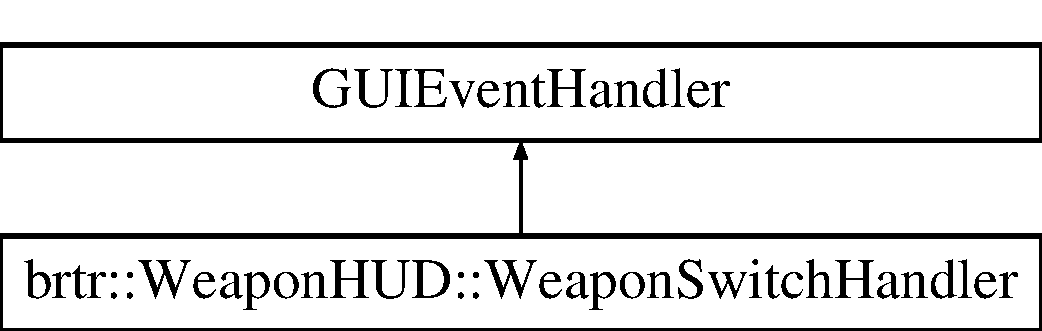
\includegraphics[height=2.000000cm]{classbrtr_1_1_weapon_h_u_d_1_1_weapon_switch_handler}
\end{center}
\end{figure}
\subsection*{Public Member Functions}
\begin{DoxyCompactItemize}
\item 
\hyperlink{classbrtr_1_1_weapon_h_u_d_1_1_weapon_switch_handler_a0f61e3aa44c58264e440186f1d7dbb0f}{Weapon\+Switch\+Handler} (Switch $\ast$switch\+Node)
\begin{DoxyCompactList}\small\item\em initializes a switch handler to switch through weapons \end{DoxyCompactList}\item 
virtual bool \hyperlink{classbrtr_1_1_weapon_h_u_d_1_1_weapon_switch_handler_ad3bd49035273e857144c1ad4927a22df}{handle} (const osg\+G\+A\+::\+G\+U\+I\+Event\+Adapter \&ea, osg\+G\+A\+::\+G\+U\+I\+Action\+Adapter \&aa)
\begin{DoxyCompactList}\small\item\em When a mouse event is triggered, this function is called to switch between weapons. \end{DoxyCompactList}\end{DoxyCompactItemize}
\subsection*{Protected Member Functions}
\begin{DoxyCompactItemize}
\item 
\hyperlink{classbrtr_1_1_weapon_h_u_d_1_1_weapon_switch_handler_a22b7a9e8884ac0c4a63979d6d441e58f}{$\sim$\+Weapon\+Switch\+Handler} ()
\end{DoxyCompactItemize}
\subsection*{Private Attributes}
\begin{DoxyCompactItemize}
\item 
ref\+\_\+ptr$<$ Switch $>$ \hyperlink{classbrtr_1_1_weapon_h_u_d_1_1_weapon_switch_handler_af4b40e431f9cbcaddf843578316bb9c4}{\+\_\+switch}
\item 
int \hyperlink{classbrtr_1_1_weapon_h_u_d_1_1_weapon_switch_handler_a15b23d25cb1847f558493adc2a97311e}{\+\_\+cur\+Weapon}
\item 
unsigned int \hyperlink{classbrtr_1_1_weapon_h_u_d_1_1_weapon_switch_handler_abfa6e6c2904d1e6ed7cd5d029a632ddf}{\+\_\+frame\+Number}
\end{DoxyCompactItemize}


\subsection{Detailed Description}
Event\+Handler for Weapon\+Switching. 

can only be obtained trough \hyperlink{classbrtr_1_1_weapon_h_u_d_a6a9a434ff3aa3861caf030763772ac74}{Weapon\+H\+U\+D\+::get\+Weapon\+Handler()} \begin{DoxyAuthor}{Author}
Jonathan Spielvogel 
\end{DoxyAuthor}
\begin{DoxyVersion}{Version}
1.\+0 
\end{DoxyVersion}
\begin{DoxyDate}{Date}
2014 
\end{DoxyDate}
\begin{DoxyCopyright}{Copyright}
G\+N\+U Public License. 
\end{DoxyCopyright}


Definition at line \hyperlink{_weapon_h_u_d_8h_source_l00032}{32} of file \hyperlink{_weapon_h_u_d_8h_source}{Weapon\+H\+U\+D.\+h}.



\subsection{Constructor \& Destructor Documentation}
\hypertarget{classbrtr_1_1_weapon_h_u_d_1_1_weapon_switch_handler_a0f61e3aa44c58264e440186f1d7dbb0f}{\index{brtr\+::\+Weapon\+H\+U\+D\+::\+Weapon\+Switch\+Handler@{brtr\+::\+Weapon\+H\+U\+D\+::\+Weapon\+Switch\+Handler}!Weapon\+Switch\+Handler@{Weapon\+Switch\+Handler}}
\index{Weapon\+Switch\+Handler@{Weapon\+Switch\+Handler}!brtr\+::\+Weapon\+H\+U\+D\+::\+Weapon\+Switch\+Handler@{brtr\+::\+Weapon\+H\+U\+D\+::\+Weapon\+Switch\+Handler}}
\subsubsection[{Weapon\+Switch\+Handler}]{\setlength{\rightskip}{0pt plus 5cm}brtr\+::\+Weapon\+H\+U\+D\+::\+Weapon\+Switch\+Handler\+::\+Weapon\+Switch\+Handler (
\begin{DoxyParamCaption}
\item[{Switch $\ast$}]{switch\+Node}
\end{DoxyParamCaption}
)}}\label{classbrtr_1_1_weapon_h_u_d_1_1_weapon_switch_handler_a0f61e3aa44c58264e440186f1d7dbb0f}


initializes a switch handler to switch through weapons 


\begin{DoxyParams}{Parameters}
{\em switch\+Node} & pointer to Switch \\
\hline
\end{DoxyParams}
\begin{DoxyReturn}{Returns}
\hyperlink{classbrtr_1_1_weapon_h_u_d_1_1_weapon_switch_handler}{Weapon\+Switch\+Handler} 
\end{DoxyReturn}


Definition at line \hyperlink{_weapon_h_u_d_8cpp_source_l00101}{101} of file \hyperlink{_weapon_h_u_d_8cpp_source}{Weapon\+H\+U\+D.\+cpp}.

\hypertarget{classbrtr_1_1_weapon_h_u_d_1_1_weapon_switch_handler_a22b7a9e8884ac0c4a63979d6d441e58f}{\index{brtr\+::\+Weapon\+H\+U\+D\+::\+Weapon\+Switch\+Handler@{brtr\+::\+Weapon\+H\+U\+D\+::\+Weapon\+Switch\+Handler}!````~Weapon\+Switch\+Handler@{$\sim$\+Weapon\+Switch\+Handler}}
\index{````~Weapon\+Switch\+Handler@{$\sim$\+Weapon\+Switch\+Handler}!brtr\+::\+Weapon\+H\+U\+D\+::\+Weapon\+Switch\+Handler@{brtr\+::\+Weapon\+H\+U\+D\+::\+Weapon\+Switch\+Handler}}
\subsubsection[{$\sim$\+Weapon\+Switch\+Handler}]{\setlength{\rightskip}{0pt plus 5cm}brtr\+::\+Weapon\+H\+U\+D\+::\+Weapon\+Switch\+Handler\+::$\sim$\+Weapon\+Switch\+Handler (
\begin{DoxyParamCaption}
{}
\end{DoxyParamCaption}
)\hspace{0.3cm}{\ttfamily [inline]}, {\ttfamily [protected]}}}\label{classbrtr_1_1_weapon_h_u_d_1_1_weapon_switch_handler_a22b7a9e8884ac0c4a63979d6d441e58f}


Definition at line \hyperlink{_weapon_h_u_d_8h_source_l00049}{49} of file \hyperlink{_weapon_h_u_d_8h_source}{Weapon\+H\+U\+D.\+h}.



\subsection{Member Function Documentation}
\hypertarget{classbrtr_1_1_weapon_h_u_d_1_1_weapon_switch_handler_ad3bd49035273e857144c1ad4927a22df}{\index{brtr\+::\+Weapon\+H\+U\+D\+::\+Weapon\+Switch\+Handler@{brtr\+::\+Weapon\+H\+U\+D\+::\+Weapon\+Switch\+Handler}!handle@{handle}}
\index{handle@{handle}!brtr\+::\+Weapon\+H\+U\+D\+::\+Weapon\+Switch\+Handler@{brtr\+::\+Weapon\+H\+U\+D\+::\+Weapon\+Switch\+Handler}}
\subsubsection[{handle}]{\setlength{\rightskip}{0pt plus 5cm}bool brtr\+::\+Weapon\+H\+U\+D\+::\+Weapon\+Switch\+Handler\+::handle (
\begin{DoxyParamCaption}
\item[{const osg\+G\+A\+::\+G\+U\+I\+Event\+Adapter \&}]{ea, }
\item[{osg\+G\+A\+::\+G\+U\+I\+Action\+Adapter \&}]{aa}
\end{DoxyParamCaption}
)\hspace{0.3cm}{\ttfamily [virtual]}}}\label{classbrtr_1_1_weapon_h_u_d_1_1_weapon_switch_handler_ad3bd49035273e857144c1ad4927a22df}


When a mouse event is triggered, this function is called to switch between weapons. 


\begin{DoxyParams}{Parameters}
{\em ea} & Gui\+Event\+Adapter \\
\hline
{\em aa} & Gui\+Action\+Adapter \\
\hline
\end{DoxyParams}
\begin{DoxyReturn}{Returns}
true, if the event was handled, otherwise false 
\end{DoxyReturn}


Definition at line \hyperlink{_weapon_h_u_d_8cpp_source_l00106}{106} of file \hyperlink{_weapon_h_u_d_8cpp_source}{Weapon\+H\+U\+D.\+cpp}.



\subsection{Member Data Documentation}
\hypertarget{classbrtr_1_1_weapon_h_u_d_1_1_weapon_switch_handler_a15b23d25cb1847f558493adc2a97311e}{\index{brtr\+::\+Weapon\+H\+U\+D\+::\+Weapon\+Switch\+Handler@{brtr\+::\+Weapon\+H\+U\+D\+::\+Weapon\+Switch\+Handler}!\+\_\+cur\+Weapon@{\+\_\+cur\+Weapon}}
\index{\+\_\+cur\+Weapon@{\+\_\+cur\+Weapon}!brtr\+::\+Weapon\+H\+U\+D\+::\+Weapon\+Switch\+Handler@{brtr\+::\+Weapon\+H\+U\+D\+::\+Weapon\+Switch\+Handler}}
\subsubsection[{\+\_\+cur\+Weapon}]{\setlength{\rightskip}{0pt plus 5cm}int brtr\+::\+Weapon\+H\+U\+D\+::\+Weapon\+Switch\+Handler\+::\+\_\+cur\+Weapon\hspace{0.3cm}{\ttfamily [private]}}}\label{classbrtr_1_1_weapon_h_u_d_1_1_weapon_switch_handler_a15b23d25cb1847f558493adc2a97311e}


Definition at line \hyperlink{_weapon_h_u_d_8h_source_l00052}{52} of file \hyperlink{_weapon_h_u_d_8h_source}{Weapon\+H\+U\+D.\+h}.

\hypertarget{classbrtr_1_1_weapon_h_u_d_1_1_weapon_switch_handler_abfa6e6c2904d1e6ed7cd5d029a632ddf}{\index{brtr\+::\+Weapon\+H\+U\+D\+::\+Weapon\+Switch\+Handler@{brtr\+::\+Weapon\+H\+U\+D\+::\+Weapon\+Switch\+Handler}!\+\_\+frame\+Number@{\+\_\+frame\+Number}}
\index{\+\_\+frame\+Number@{\+\_\+frame\+Number}!brtr\+::\+Weapon\+H\+U\+D\+::\+Weapon\+Switch\+Handler@{brtr\+::\+Weapon\+H\+U\+D\+::\+Weapon\+Switch\+Handler}}
\subsubsection[{\+\_\+frame\+Number}]{\setlength{\rightskip}{0pt plus 5cm}unsigned int brtr\+::\+Weapon\+H\+U\+D\+::\+Weapon\+Switch\+Handler\+::\+\_\+frame\+Number\hspace{0.3cm}{\ttfamily [private]}}}\label{classbrtr_1_1_weapon_h_u_d_1_1_weapon_switch_handler_abfa6e6c2904d1e6ed7cd5d029a632ddf}


Definition at line \hyperlink{_weapon_h_u_d_8h_source_l00053}{53} of file \hyperlink{_weapon_h_u_d_8h_source}{Weapon\+H\+U\+D.\+h}.

\hypertarget{classbrtr_1_1_weapon_h_u_d_1_1_weapon_switch_handler_af4b40e431f9cbcaddf843578316bb9c4}{\index{brtr\+::\+Weapon\+H\+U\+D\+::\+Weapon\+Switch\+Handler@{brtr\+::\+Weapon\+H\+U\+D\+::\+Weapon\+Switch\+Handler}!\+\_\+switch@{\+\_\+switch}}
\index{\+\_\+switch@{\+\_\+switch}!brtr\+::\+Weapon\+H\+U\+D\+::\+Weapon\+Switch\+Handler@{brtr\+::\+Weapon\+H\+U\+D\+::\+Weapon\+Switch\+Handler}}
\subsubsection[{\+\_\+switch}]{\setlength{\rightskip}{0pt plus 5cm}ref\+\_\+ptr$<$Switch$>$ brtr\+::\+Weapon\+H\+U\+D\+::\+Weapon\+Switch\+Handler\+::\+\_\+switch\hspace{0.3cm}{\ttfamily [private]}}}\label{classbrtr_1_1_weapon_h_u_d_1_1_weapon_switch_handler_af4b40e431f9cbcaddf843578316bb9c4}


Definition at line \hyperlink{_weapon_h_u_d_8h_source_l00051}{51} of file \hyperlink{_weapon_h_u_d_8h_source}{Weapon\+H\+U\+D.\+h}.



The documentation for this class was generated from the following files\+:\begin{DoxyCompactItemize}
\item 
header/\hyperlink{_weapon_h_u_d_8h}{Weapon\+H\+U\+D.\+h}\item 
Camera/\hyperlink{_weapon_h_u_d_8cpp}{Weapon\+H\+U\+D.\+cpp}\end{DoxyCompactItemize}

\chapter{File Documentation}
\hypertarget{_animation_creater_8cpp}{\section{Animation/\+Animation\+Creater.cpp File Reference}
\label{_animation_creater_8cpp}\index{Animation/\+Animation\+Creater.\+cpp@{Animation/\+Animation\+Creater.\+cpp}}
}
{\ttfamily \#include \char`\"{}../header/\+Animation\+Creater.\+h\char`\"{}}\\*
{\ttfamily \#include $<$osg\+Viewer/\+Viewer$>$}\\*
{\ttfamily \#include $<$osg/\+Geometry$>$}\\*
{\ttfamily \#include $<$osg\+D\+B/\+Read\+File$>$}\\*
{\ttfamily \#include $<$osg/\+Blend\+Func$>$}\\*
{\ttfamily \#include $<$osg/\+Value\+Object$>$}\\*
{\ttfamily \#include $<$osg\+Util/\+Optimizer$>$}\\*
{\ttfamily \#include $<$osg/\+Animation\+Path$>$}\\*
{\ttfamily \#include $<$osg/\+Matrix\+Transform$>$}\\*
{\ttfamily \#include $<$cmath$>$}\\*

\hypertarget{_animation_creater_8cpp_source}{\section{Animation\+Creater.\+cpp}
\label{_animation_creater_8cpp_source}\index{Animation/\+Animation\+Creater.\+cpp@{Animation/\+Animation\+Creater.\+cpp}}
}

\begin{DoxyCode}
00001 \textcolor{preprocessor}{#include "../header/AnimationCreater.h"}
00002 \textcolor{preprocessor}{#include <osgViewer/Viewer>}
00003 \textcolor{preprocessor}{#include <osg/Geometry>}
00004 \textcolor{preprocessor}{#include <osgDB/ReadFile>}
00005 \textcolor{preprocessor}{#include <osg/BlendFunc>}
00006 \textcolor{preprocessor}{#include <osg/ValueObject>}
00007 \textcolor{preprocessor}{#include <osgUtil/Optimizer>}
00008 \textcolor{preprocessor}{#include <osg/AnimationPath>}
00009 \textcolor{preprocessor}{#include <osg/MatrixTransform>}
00010 \textcolor{preprocessor}{#include <cmath>}
00011 \textcolor{keyword}{using namespace }osg;
00012 
00013 \textcolor{comment}{/*calculates the angle between two points and return the angle as radian.}
00014 \textcolor{comment}{ *not in use.}
00015 \textcolor{comment}{ */}
\hypertarget{_animation_creater_8cpp_source_l00016}{}\hyperlink{class_animation_creator_a03e8400c38e8710ee20fd44f57ab1903}{00016} \textcolor{keywordtype}{double} \hyperlink{class_animation_creator_a03e8400c38e8710ee20fd44f57ab1903}{AnimationCreator::getAngleRad}(Vec3 pointA, Vec3 pointB) \{
00017     \textcolor{keywordtype}{int} kurvenFaktor = 1; \textcolor{comment}{//a factor for bigger angles, if necessary.}
00018     
00019     \textcolor{keywordtype}{double} dotProd = pointA.x() * pointB.x() + pointA.y() * pointB.y() + pointA.z() * pointB.z();
00020     \textcolor{keywordtype}{double} lengthA = sqrt(pointA.x() * pointA.x() + pointA.y() * pointA.y() + pointA.z() * pointA.z());
00021     \textcolor{keywordtype}{double} lengthB = sqrt(pointB.x() * pointB.x() + pointB.y() * pointB.y() + pointB.z() * pointB.z());
00022 
00023     \textcolor{comment}{//if (skalarProd == 0)}
00024      \textcolor{comment}{//   return acos(0);}
00025 
00026     \textcolor{keywordtype}{double} result = dotProd / (lengthA * lengthB);
00027     \textcolor{keywordflow}{return} osg::DegreesToRadians(acos(result))*kurvenFaktor *  1;
00028 \}
00029 
00030 \textcolor{comment}{/*}
00031 \textcolor{comment}{}
00032 \textcolor{comment}{Method construct's the AnimationPath for the Train.}
00033 \textcolor{comment}{Time = time that the train will take between two points.}
00034 \textcolor{comment}{}
00035 \textcolor{comment}{loading a file must be looking like this:}
00036 \textcolor{comment}{osgDB::readNodeFile("..path../Train.ive.0,0,-48.rot");}
00037 \textcolor{comment}{}
00038 \textcolor{comment}{*/}
00039 
\hypertarget{_animation_creater_8cpp_source_l00040}{}\hyperlink{class_animation_creator_aca52f3472d0be7043c63ff5ede8084aa}{00040} osg::AnimationPath* \hyperlink{class_animation_creator_aca52f3472d0be7043c63ff5ede8084aa}{AnimationCreator::createAnimationPath}(\textcolor{keywordtype}{float} time) 
      \{
00041     \textcolor{keywordtype}{int} vectorCount = 10; \textcolor{comment}{//witch points will be used, in this case every 10th point.}
00042     osg::ref\_ptr<osg::AnimationPath> path = \textcolor{keyword}{new} osg::AnimationPath;
00043     path->setLoopMode(osg::AnimationPath::LOOP);
00044 
00045     \textcolor{comment}{//array constructed with script.}
00046     Vec3 pathArray[] = \{
00047         Vec3(-187.90732, 43.37911, -4.13946),
00048         Vec3(-150.33286, -2.83142, -4.13946),
00049         Vec3(-149.98206, -3.25188, -4.13945),
00050         Vec3(-149.78517, -3.09980, -4.13945),
00051         Vec3(-150.13493, -2.68066, -4.13946),
00052         Vec3(-149.61302, -3.70120, -4.13945),
00053         Vec3(-149.41745, -3.54740, -4.13945),
00054         Vec3(-149.21957, -4.18303, -4.13944),
00055         Vec3(-149.02556, -4.02728, -4.13944),
00056         Vec3(-148.79701, -4.69947, -4.13943),
00057         Vec3(-148.60464, -4.54167, -4.13943),
00058         Vec3(-148.34061, -5.25264, -4.13943),
00059         Vec3(-148.14992, -5.09283, -4.13943),
00060         Vec3(-147.84575, -5.84474, -4.13942),
00061         Vec3(-147.65660, -5.68308, -4.13942),
00062         Vec3(-147.30782, -6.47796, -4.13940),
00063         Vec3(-147.12001, -6.31475, -4.13940),
00064         Vec3(-146.72226, -7.15456, -4.13939),
00065         Vec3(-146.53545, -6.99021, -4.13939),
00066         Vec3(-146.72226, -7.15456, -4.13939),
00067         Vec3(-146.08452, -7.87678, -4.13937),
00068         Vec3(-145.89822, -7.71182, -4.13937),
00069         Vec3(-146.53545, -6.99021, -4.13939),
00070         Vec3(-146.08452, -7.87678, -4.13937),
00071         Vec3(-145.45525, -8.47080, -4.13933),
00072         Vec3(-145.27003, -8.30459, -4.13933),
00073         Vec3(-145.89822, -7.71182, -4.13937),
00074         Vec3(-145.45525, -8.47080, -4.13933),
00075         Vec3(-144.95224, -9.02164, -4.13931),
00076         Vec3(-144.76845, -8.85387, -4.13931),
00077         Vec3(-145.27003, -8.30459, -4.13933),
00078         Vec3(-144.44533, -9.56906, -4.13929),
00079         Vec3(-144.26297, -9.39972, -4.13929),
00080         Vec3(-143.93442, -10.11294, -4.13927),
00081         Vec3(-143.75352, -9.94201, -4.13927),
00082         Vec3(-143.41940, -10.65314, -4.13925),
00083         Vec3(-143.24002, -10.48063, -4.13925),
00084         Vec3(-142.90018, -11.18955, -4.13923),
00085         Vec3(-142.72232, -11.01544, -4.13923),
00086         Vec3(-142.37665, -11.72202, -4.13921),
00087         Vec3(-142.20035, -11.54632, -4.13921),
00088         Vec3(-141.84869, -12.25044, -4.13919),
00089         Vec3(-141.67400, -12.07312, -4.13919),
00090         Vec3(-141.31621, -12.77466, -4.13917),
00091         Vec3(-141.14317, -12.59573, -4.13917),
00092         Vec3(-140.77911, -13.29456, -4.13915),
00093         Vec3(-140.60776, -13.11401, -4.13915),
00094         Vec3(-140.23730, -13.80999, -4.13913),
00095         Vec3(-140.06766, -13.62782, -4.13913),
00096         Vec3(-140.23730, -13.80999, -4.13913),
00097         Vec3(-139.69070, -14.32080, -4.13911),
00098         Vec3(-139.52281, -14.13699, -4.13911),
00099         Vec3(-140.06766, -13.62782, -4.13913),
00100         Vec3(-139.69070, -14.32080, -4.13911),
00101         Vec3(-139.13924, -14.82681, -4.13910),
00102         Vec3(-138.97314, -14.64136, -4.13910),
00103         Vec3(-139.52281, -14.13699, -4.13911),
00104         Vec3(-138.58282, -15.32785, -4.13909),
00105         Vec3(-138.41858, -15.14077, -4.13909),
00106         Vec3(-138.02141, -15.82376, -4.13908),
00107         Vec3(-137.85905, -15.63502, -4.13908),
00108         Vec3(-138.02141, -15.82376, -4.13908),
00109         Vec3(-137.45491, -16.31435, -4.13908),
00110         Vec3(-137.29449, -16.12397, -4.13908),
00111         Vec3(-137.85905, -15.63502, -4.13908),
00112         Vec3(-136.88326, -16.79946, -4.13908),
00113         Vec3(-136.72482, -16.60743, -4.13908),
00114         Vec3(-136.88326, -16.79946, -4.13908),
00115         Vec3(-136.30638, -17.27891, -4.13909),
00116         Vec3(-136.14998, -17.08523, -4.13909),
00117         Vec3(-136.72482, -16.60743, -4.13908),
00118         Vec3(-135.72421, -17.75254, -4.13910),
00119         Vec3(-135.56987, -17.55721, -4.13910),
00120         Vec3(-135.72421, -17.75254, -4.13910),
00121         Vec3(-135.13667, -18.22016, -4.13912),
00122         Vec3(-134.98445, -18.02318, -4.13912),
00123         Vec3(-135.56987, -17.55721, -4.13910),
00124         Vec3(-135.13667, -18.22016, -4.13912),
00125         Vec3(-134.54373, -18.68158, -4.13914),
00126         Vec3(-134.39369, -18.48295, -4.13914),
00127         Vec3(-134.98445, -18.02318, -4.13912),
00128         Vec3(-133.94537, -19.13657, -4.13917),
00129         Vec3(-133.79756, -18.93630, -4.13917),
00130         Vec3(-133.94537, -19.13657, -4.13917),
00131         Vec3(-133.34160, -19.58493, -4.13920),
00132         Vec3(-133.19604, -19.38301, -4.13920),
00133         Vec3(-133.79756, -18.93630, -4.13917),
00134         Vec3(-133.34160, -19.58493, -4.13920),
00135         Vec3(-132.73238, -20.02643, -4.13924),
00136         Vec3(-132.58914, -19.82288, -4.13924),
00137         Vec3(-133.19604, -19.38301, -4.13920),
00138         Vec3(-132.11769, -20.46085, -4.13927),
00139         Vec3(-131.97684, -20.25568, -4.13927),
00140         Vec3(-131.49753, -20.88799, -4.13931),
00141         Vec3(-131.35910, -20.68119, -4.13931),
00142         Vec3(-131.49753, -20.88799, -4.13931),
00143         Vec3(-130.87189, -21.30762, -4.13934),
00144         Vec3(-130.73592, -21.09921, -4.13934),
00145         Vec3(-131.35910, -20.68119, -4.13931),
00146         Vec3(-130.87189, -21.30762, -4.13934),
00147         Vec3(-130.24074, -21.71952, -4.13937),
00148         Vec3(-130.10728, -21.50951, -4.13937),
00149         Vec3(-130.73592, -21.09921, -4.13934),
00150         Vec3(-129.60408, -22.12349, -4.13939),
00151         Vec3(-129.47318, -21.91189, -4.13939),
00152         Vec3(-129.60408, -22.12349, -4.13939),
00153         Vec3(-128.96194, -22.51934, -4.13941),
00154         Vec3(-128.83365, -22.30616, -4.13941),
00155         Vec3(-129.47318, -21.91189, -4.13939),
00156         Vec3(-128.31442, -22.90694, -4.13943),
00157         Vec3(-128.18878, -22.69220, -4.13943),
00158         Vec3(-128.31442, -22.90694, -4.13943),
00159         Vec3(-127.66164, -23.28616, -4.13944),
00160         Vec3(-127.53868, -23.06987, -4.13944),
00161         Vec3(-128.18878, -22.69220, -4.13943),
00162         Vec3(-127.66164, -23.28616, -4.13944),
00163         Vec3(-127.00371, -23.65688, -4.13945),
00164         Vec3(-126.88348, -23.43906, -4.13945),
00165         Vec3(-127.53868, -23.06987, -4.13944),
00166         Vec3(-126.34073, -24.01897, -4.13945),
00167         Vec3(-126.22327, -23.79964, -4.13945),
00168         Vec3(-126.34073, -24.01897, -4.13945),
00169         Vec3(-125.67283, -24.37230, -4.13946),
00170         Vec3(-125.55818, -24.15150, -4.13946),
00171         Vec3(-126.22327, -23.79964, -4.13945),
00172         Vec3(-125.00011, -24.71677, -4.13946),
00173         Vec3(-124.88832, -24.49451, -4.13946),
00174         Vec3(-124.32271, -25.05223, -4.13946),
00175         Vec3(-124.21379, -24.82856, -4.13946),
00176         Vec3(-123.64072, -25.37859, -4.13946),
00177         Vec3(-123.53471, -25.15351, -4.13946),
00178         Vec3(-122.95428, -25.69571, -4.13946),
00179         Vec3(-122.85121, -25.46927, -4.13946),
00180         Vec3(-122.26353, -26.00356, -4.13946),
00181         Vec3(-122.16344, -25.77580, -4.13946),
00182         Vec3(-121.56863, -26.30214, -4.13946),
00183         Vec3(-121.47153, -26.07308, -4.13946),
00184         Vec3(-120.86975, -26.59141, -4.13946),
00185         Vec3(-120.77567, -26.36110, -4.13946),
00186         Vec3(-120.16704, -26.87136, -4.13946),
00187         Vec3(-120.07599, -26.63983, -4.13946),
00188         Vec3(-119.46065, -27.14198, -4.13946),
00189         Vec3(-119.37265, -26.90927, -4.13946),
00190         Vec3(-118.75076, -27.40325, -4.13946),
00191         Vec3(-118.66583, -27.16941, -4.13946),
00192         Vec3(-118.03752, -27.65516, -4.13946),
00193         Vec3(-117.95568, -27.42022, -4.13946),
00194         Vec3(-117.32111, -27.89770, -4.13946),
00195         Vec3(-117.24235, -27.66170, -4.13946),
00196         Vec3(-116.60166, -28.13085, -4.13946),
00197         Vec3(-116.52600, -27.89385, -4.13946),
00198         Vec3(-115.87935, -28.35463, -4.13946),
00199         Vec3(-115.80679, -28.11666, -4.13946),
00200         Vec3(-115.15433, -28.56903, -4.13946),
00201         Vec3(-115.08487, -28.33014, -4.13946),
00202         Vec3(-114.42673, -28.77409, -4.13946),
00203         Vec3(-114.36037, -28.53431, -4.13946),
00204         Vec3(-113.69670, -28.96981, -4.13946),
00205         Vec3(-113.63344, -28.72920, -4.13946),
00206         Vec3(-112.96441, -29.15620, -4.13946),
00207         Vec3(-112.90424, -28.91480, -4.13946),
00208         Vec3(-112.23000, -29.33329, -4.13946),
00209         Vec3(-112.17290, -29.09115, -4.13946),
00210         Vec3(-111.49360, -29.50111, -4.13946),
00211         Vec3(-111.43956, -29.25826, -4.13946),
00212         Vec3(-110.75537, -29.65965, -4.13946),
00213         Vec3(-110.70438, -29.41615, -4.13946),
00214         Vec3(-110.01547, -29.80896, -4.13946),
00215         Vec3(-109.96751, -29.56484, -4.13946),
00216         Vec3(-109.27403, -29.94905, -4.13946),
00217         Vec3(-109.22908, -29.70436, -4.13946),
00218         Vec3(-108.53119, -30.08001, -4.13946),
00219         Vec3(-108.48923, -29.83479, -4.13946),
00220         Vec3(-107.78709, -30.20189, -4.13946),
00221         Vec3(-107.74808, -29.95618, -4.13946),
00222         Vec3(-107.04185, -30.31478, -4.13946),
00223         Vec3(-107.00578, -30.06862, -4.13946),
00224         Vec3(-106.29562, -30.41875, -4.13946),
00225         Vec3(-106.26244, -30.17219, -4.13946),
00226         Vec3(-105.54852, -30.51389, -4.13946),
00227         Vec3(-105.51822, -30.26695, -4.13946),
00228         Vec3(-104.80069, -30.60025, -4.13946),
00229         Vec3(-104.77322, -30.35299, -4.13946),
00230         Vec3(-104.05226, -30.67794, -4.13946),
00231         Vec3(-104.02759, -30.43037, -4.13946),
00232         Vec3(-103.30337, -30.74701, -4.13946),
00233         Vec3(-103.28145, -30.49919, -4.13946),
00234         Vec3(-102.55413, -30.80756, -4.13946),
00235         Vec3(-102.53493, -30.55951, -4.13946),
00236         Vec3(-101.80469, -30.85971, -4.13946),
00237         Vec3(-101.78815, -30.61148, -4.13946),
00238         Vec3(-101.05508, -30.90365, -4.13946),
00239         Vec3(-101.04119, -30.65525, -4.13946),
00240         Vec3(-100.30545, -30.93952, -4.13946),
00241         Vec3(-100.29414, -30.69099, -4.13946),
00242         Vec3(-99.55585, -30.96750, -4.13946),
00243         Vec3(-99.54707, -30.71887, -4.13946),
00244         Vec3(-98.80640, -30.98776, -4.13946),
00245         Vec3(-98.80012, -30.73905, -4.13946),
00246         Vec3(-98.05717, -31.00046, -4.13946),
00247         Vec3(-98.05334, -30.75170, -4.13946),
00248         Vec3(-97.30827, -31.00576, -4.13946),
00249         Vec3(-97.30684, -30.75698, -4.13946),
00250         Vec3(-96.55977, -31.00385, -4.13946),
00251         Vec3(-96.56069, -30.75506, -4.13946),
00252         Vec3(-95.81177, -30.99488, -4.13946),
00253         Vec3(-95.81499, -30.74611, -4.13946),
00254         Vec3(-95.06435, -30.97901, -4.13946),
00255         Vec3(-95.06982, -30.73028, -4.13946),
00256         Vec3(-94.31756, -30.95643, -4.13946),
00257         Vec3(-94.32523, -30.70776, -4.13946),
00258         Vec3(-93.57141, -30.92729, -4.13946),
00259         Vec3(-93.58124, -30.67870, -4.13946),
00260         Vec3(-92.82597, -30.89177, -4.13946),
00261         Vec3(-92.83791, -30.64327, -4.13946),
00262         Vec3(-92.08128, -30.85004, -4.13946),
00263         Vec3(-92.09526, -30.60165, -4.13946),
00264         Vec3(-91.33737, -30.80227, -4.13946),
00265         Vec3(-91.35335, -30.55399, -4.13946),
00266         Vec3(-90.59427, -30.74861, -4.13946),
00267         Vec3(-90.61221, -30.50047, -4.13946),
00268         Vec3(-89.85204, -30.68924, -4.13946),
00269         Vec3(-89.87189, -30.44125, -4.13946),
00270         Vec3(-89.11073, -30.62434, -4.13946),
00271         Vec3(-89.13242, -30.37650, -4.13946),
00272         Vec3(-88.37035, -30.55405, -4.13946),
00273         Vec3(-88.39384, -30.30638, -4.13946),
00274         Vec3(-87.63091, -30.47854, -4.13946),
00275         Vec3(-87.65617, -30.23104, -4.13946),
00276         Vec3(-86.89246, -30.39795, -4.13946),
00277         Vec3(-86.91942, -30.15062, -4.13946),
00278         Vec3(-86.15496, -30.31242, -4.13946),
00279         Vec3(-86.18358, -30.06529, -4.13946),
00280         Vec3(-85.41846, -30.22211, -4.13946),
00281         Vec3(-85.44870, -29.97517, -4.13946),
00282         Vec3(-84.68295, -30.12716, -4.13946),
00283         Vec3(-84.71474, -29.88041, -4.13946),
00284         Vec3(-83.94843, -30.02770, -4.13946),
00285         Vec3(-83.98175, -29.78115, -4.13946),
00286         Vec3(-83.21492, -29.92390, -4.13946),
00287         Vec3(-83.24971, -29.67756, -4.13946),
00288         Vec3(-82.48243, -29.81588, -4.13946),
00289         Vec3(-82.51865, -29.56974, -4.13946),
00290         Vec3(-81.75096, -29.70380, -4.13946),
00291         Vec3(-81.78856, -29.45787, -4.13946),
00292         Vec3(-81.02052, -29.58780, -4.13946),
00293         Vec3(-81.05946, -29.34208, -4.13946),
00294         Vec3(-80.29109, -29.46799, -4.13946),
00295         Vec3(-80.33132, -29.22248, -4.13946),
00296         Vec3(-79.56268, -29.34452, -4.13946),
00297         Vec3(-79.60416, -29.09921, -4.13946),
00298         Vec3(-78.83524, -29.21750, -4.13946),
00299         Vec3(-78.87793, -28.97240, -4.13946),
00300         Vec3(-78.10879, -29.08706, -4.13946),
00301         Vec3(-78.15264, -28.84217, -4.13946),
00302         Vec3(-77.38332, -28.95333, -4.13946),
00303         Vec3(-77.42830, -28.70864, -4.13946),
00304         Vec3(-76.65880, -28.81644, -4.13946),
00305         Vec3(-76.70486, -28.57195, -4.13946),
00306         Vec3(-75.93525, -28.67651, -4.13946),
00307         Vec3(-75.98235, -28.43222, -4.13946),
00308         Vec3(-75.21263, -28.53366, -4.13946),
00309         Vec3(-75.26073, -28.28957, -4.13946),
00310         Vec3(-74.49094, -28.38802, -4.13946),
00311         Vec3(-74.54001, -28.14412, -4.13946),
00312         Vec3(-73.77016, -28.23971, -4.13946),
00313         Vec3(-73.82015, -27.99600, -4.13946),
00314         Vec3(-73.05026, -28.08883, -4.13946),
00315         Vec3(-73.10114, -27.84530, -4.13946),
00316         Vec3(-72.33125, -27.93550, -4.13946),
00317         Vec3(-72.38298, -27.69214, -4.13946),
00318         Vec3(-71.61310, -27.77981, -4.13946),
00319         Vec3(-71.66563, -27.53663, -4.13946),
00320         Vec3(-70.89577, -27.62188, -4.13946),
00321         Vec3(-70.94907, -27.37887, -4.13946),
00322         Vec3(-70.17924, -27.46183, -4.13946),
00323         Vec3(-70.23329, -27.21898, -4.13946),
00324         Vec3(-69.46352, -27.29975, -4.13946),
00325         Vec3(-69.51826, -27.05706, -4.13946),
00326         Vec3(-68.74855, -27.13575, -4.13946),
00327         Vec3(-68.80396, -26.89322, -4.13946),
00328         Vec3(-68.03434, -26.96996, -4.13946),
00329         Vec3(-68.09039, -26.72756, -4.13946),
00330         Vec3(-67.32086, -26.80245, -4.13946),
00331         Vec3(-67.37750, -26.56020, -4.13946),
00332         Vec3(-66.60809, -26.63334, -4.13946),
00333         Vec3(-66.66530, -26.39121, -4.13946),
00334         Vec3(-65.89600, -26.46270, -4.13946),
00335         Vec3(-65.95374, -26.22071, -4.13946),
00336         Vec3(-65.18456, -26.29065, -4.13946),
00337         Vec3(-65.24280, -26.04878, -4.13946),
00338         Vec3(-64.47375, -26.11728, -4.13946),
00339         Vec3(-64.53246, -25.87551, -4.13946),
00340         Vec3(-63.76357, -25.94267, -4.13946),
00341         Vec3(-63.82272, -25.70101, -4.13946),
00342         Vec3(-63.05398, -25.76692, -4.13946),
00343         Vec3(-63.11353, -25.52536, -4.13946),
00344         Vec3(-62.34494, -25.59013, -4.13946),
00345         Vec3(-62.40486, -25.34866, -4.13946),
00346         Vec3(-61.63643, -25.41239, -4.13946),
00347         Vec3(-61.69669, -25.17101, -4.13946),
00348         Vec3(-60.92844, -25.23379, -4.13946),
00349         Vec3(-60.98901, -24.99249, -4.13946),
00350         Vec3(-60.22095, -25.05441, -4.13946),
00351         Vec3(-60.28181, -24.81318, -4.13946),
00352         Vec3(-59.51392, -24.87435, -4.13946),
00353         Vec3(-59.57503, -24.63318, -4.13946),
00354         Vec3(-58.80734, -24.69367, -4.13946),
00355         Vec3(-58.86867, -24.45256, -4.13946),
00356         Vec3(-58.10118, -24.51248, -4.13946),
00357         Vec3(-58.16270, -24.27142, -4.13946),
00358         Vec3(-57.39542, -24.33084, -4.13946),
00359         Vec3(-57.45712, -24.08982, -4.13946),
00360         Vec3(-56.69004, -24.14885, -4.13946),
00361         Vec3(-56.75186, -23.90786, -4.13946),
00362         Vec3(-55.98500, -23.96658, -4.13946),
00363         Vec3(-56.04694, -23.72562, -4.13946),
00364         Vec3(-55.28028, -23.78412, -4.13946),
00365         Vec3(-55.34230, -23.54319, -4.13946),
00366         Vec3(-54.57589, -23.60155, -4.13946),
00367         Vec3(-54.63795, -23.36063, -4.13946),
00368         Vec3(-53.87176, -23.41895, -4.13946),
00369         Vec3(-53.93385, -23.17804, -4.13946),
00370         Vec3(-53.16788, -23.23639, -4.13946),
00371         Vec3(-53.22997, -22.99548, -4.13946),
00372         Vec3(-52.46425, -23.05395, -4.13946),
00373         Vec3(-52.52631, -22.81303, -4.13946),
00374         Vec3(-51.76084, -22.87171, -4.13946),
00375         Vec3(-51.82285, -22.63077, -4.13946),
00376         Vec3(-51.05760, -22.68973, -4.13946),
00377         Vec3(-51.11954, -22.44877, -4.13946),
00378         Vec3(-50.35458, -22.50809, -4.13946),
00379         Vec3(-50.41640, -22.26711, -4.13946),
00380         Vec3(-49.65166, -22.32687, -4.13946),
00381         Vec3(-49.71337, -22.08586, -4.13946),
00382         Vec3(-48.94891, -22.14615, -4.13946),
00383         Vec3(-49.01045, -21.90509, -4.13946),
00384         Vec3(-48.24623, -21.96599, -4.13946),
00385         Vec3(-48.30759, -21.72489, -4.13946),
00386         Vec3(-47.54365, -21.78647, -4.13946),
00387         Vec3(-47.60481, -21.54531, -4.13946),
00388         Vec3(-46.84115, -21.60765, -4.13946),
00389         Vec3(-46.90208, -21.36644, -4.13946),
00390         Vec3(-46.13870, -21.42962, -4.13946),
00391         Vec3(-46.19938, -21.18834, -4.13946),
00392         Vec3(-45.43626, -21.25243, -4.13946),
00393         Vec3(-45.49667, -21.01108, -4.13946),
00394         Vec3(-44.73387, -21.07615, -4.13946),
00395         Vec3(-44.79397, -20.83472, -4.13946),
00396         Vec3(-44.03144, -20.90084, -4.13946),
00397         Vec3(-44.09122, -20.65934, -4.13946),
00398         Vec3(-43.32903, -20.72659, -4.13946),
00399         Vec3(-43.38844, -20.48500, -4.13946),
00400         Vec3(-42.62653, -20.55345, -4.13946),
00401         Vec3(-42.68559, -20.31178, -4.13946),
00402         Vec3(-41.92402, -20.38150, -4.13946),
00403         Vec3(-41.98267, -20.13973, -4.13946),
00404         Vec3(-41.22142, -20.21080, -4.13946),
00405         Vec3(-41.27966, -19.96892, -4.13946),
00406         Vec3(-40.51873, -20.04142, -4.13946),
00407         Vec3(-40.57652, -19.79943, -4.13946),
00408         Vec3(-39.81596, -19.87341, -4.13946),
00409         Vec3(-39.87328, -19.63132, -4.13946),
00410         Vec3(-39.11304, -19.70685, -4.13946),
00411         Vec3(-39.16988, -19.46464, -4.13946),
00412         Vec3(-38.41002, -19.54178, -4.13946),
00413         Vec3(-38.46635, -19.29946, -4.13946),
00414         Vec3(-37.70686, -19.37829, -4.13946),
00415         Vec3(-37.76265, -19.13584, -4.13946),
00416         Vec3(-37.00352, -19.21642, -4.13946),
00417         Vec3(-37.05876, -18.97384, -4.13946),
00418         Vec3(-36.30002, -19.05623, -4.13946),
00419         Vec3(-36.35469, -18.81353, -4.13946),
00420         Vec3(-35.59637, -18.89780, -4.13946),
00421         Vec3(-35.65044, -18.65496, -4.13946),
00422         Vec3(-34.89249, -18.74119, -4.13946),
00423         Vec3(-34.94594, -18.49821, -4.13946),
00424         Vec3(-34.18842, -18.58644, -4.13946),
00425         Vec3(-34.24123, -18.34333, -4.13946),
00426         Vec3(-33.48412, -18.43363, -4.13946),
00427         Vec3(-33.53626, -18.19037, -4.13946),
00428         Vec3(-32.77962, -18.28280, -4.13946),
00429         Vec3(-32.83109, -18.03940, -4.13946),
00430         Vec3(-32.07490, -18.13402, -4.13946),
00431         Vec3(-32.12566, -17.89046, -4.13946),
00432         Vec3(-31.36991, -17.98733, -4.13946),
00433         Vec3(-31.41996, -17.74363, -4.13946),
00434         Vec3(-30.66471, -17.84280, -4.13946),
00435         Vec3(-30.71401, -17.59894, -4.13946),
00436         Vec3(-29.95924, -17.70047, -4.13946),
00437         Vec3(-30.00778, -17.45647, -4.13946),
00438         Vec3(-29.25352, -17.56042, -4.13946),
00439         Vec3(-29.30128, -17.31626, -4.13946),
00440         Vec3(-28.54752, -17.42268, -4.13946),
00441         Vec3(-28.59448, -17.17837, -4.13946),
00442         Vec3(-27.84126, -17.28733, -4.13946),
00443         Vec3(-27.88741, -17.04285, -4.13946),
00444         Vec3(-27.13472, -17.15440, -4.13946),
00445         Vec3(-27.18002, -16.90977, -4.13946),
00446         Vec3(-26.42790, -17.02394, -4.13946),
00447         Vec3(-26.47234, -16.77916, -4.13946),
00448         Vec3(-25.72080, -16.89602, -4.13946),
00449         Vec3(-25.76437, -16.65107, -4.13946),
00450         Vec3(-25.01343, -16.77067, -4.13946),
00451         Vec3(-25.05610, -16.52557, -4.13946),
00452         Vec3(-24.30576, -16.64793, -4.13946),
00453         Vec3(-24.34752, -16.40268, -4.13946),
00454         Vec3(-23.59780, -16.52788, -4.13946),
00455         Vec3(-23.63863, -16.28246, -4.13946),
00456         Vec3(-22.88956, -16.41054, -4.13946),
00457         Vec3(-22.92945, -16.16497, -4.13946),
00458         Vec3(-22.18101, -16.29597, -4.13946),
00459         Vec3(-22.21993, -16.05025, -4.13946),
00460         Vec3(-21.47219, -16.18422, -4.13946),
00461         Vec3(-21.51013, -15.93834, -4.13946),
00462         Vec3(-20.76305, -16.07533, -4.13946),
00463         Vec3(-20.80001, -15.82930, -4.13946),
00464         Vec3(-20.05367, -15.96935, -4.13946),
00465         Vec3(-20.08961, -15.72317, -4.13946),
00466         Vec3(-19.34396, -15.86630, -4.13946),
00467         Vec3(-19.37888, -15.61998, -4.13946),
00468         Vec3(-18.63399, -15.76624, -4.13946),
00469         Vec3(-18.66786, -15.51977, -4.13946),
00470         Vec3(-17.92374, -15.66920, -4.13946),
00471         Vec3(-17.95656, -15.42259, -4.13946),
00472         Vec3(-17.21323, -15.57522, -4.13946),
00473         Vec3(-17.24498, -15.32846, -4.13946),
00474         Vec3(-16.50244, -15.48434, -4.13946),
00475         Vec3(-16.53310, -15.23745, -4.13946),
00476         Vec3(-15.79137, -15.39660, -4.13946),
00477         Vec3(-15.82092, -15.14958, -4.13946),
00478         Vec3(-15.08005, -15.31205, -4.13946),
00479         Vec3(-15.10849, -15.06489, -4.13946),
00480         Vec3(-14.36845, -15.23071, -4.13946),
00481         Vec3(-14.39578, -14.98343, -4.13946),
00482         Vec3(-13.65663, -15.15262, -4.13946),
00483         Vec3(-13.68283, -14.90521, -4.13946),
00484         Vec3(-12.94453, -15.07780, -4.13946),
00485         Vec3(-12.96957, -14.83028, -4.13946),
00486         Vec3(-12.23227, -15.00630, -4.13946),
00487         Vec3(-12.25615, -14.75866, -4.13946),
00488         Vec3(-11.51973, -14.93812, -4.13946),
00489         Vec3(-11.54243, -14.69037, -4.13946),
00490         Vec3(-10.80698, -14.87331, -4.13946),
00491         Vec3(-10.82849, -14.62545, -4.13946),
00492         Vec3(-10.09402, -14.81189, -4.13946),
00493         Vec3(-10.11435, -14.56393, -4.13946),
00494         Vec3(-9.38087, -14.75389, -4.13946),
00495         Vec3(-9.40001, -14.50584, -4.13946),
00496         Vec3(-8.66753, -14.69934, -4.13946),
00497         Vec3(-8.68546, -14.45120, -4.13946),
00498         Vec3(-7.95398, -14.64827, -4.13946),
00499         Vec3(-7.97069, -14.40004, -4.13946),
00500         Vec3(-7.24028, -14.60071, -4.13946),
00501         Vec3(-7.25577, -14.35240, -4.13946),
00502         Vec3(-6.52640, -14.55670, -4.13946),
00503         Vec3(-6.54065, -14.30832, -4.13946),
00504         Vec3(-5.81241, -14.51627, -4.13946),
00505         Vec3(-5.82541, -14.26782, -4.13946),
00506         Vec3(-5.09825, -14.47946, -4.13946),
00507         Vec3(-5.11002, -14.23095, -4.13946),
00508         Vec3(-4.38396, -14.44630, -4.13946),
00509         Vec3(-4.39449, -14.19774, -4.13946),
00510         Vec3(-3.66957, -14.41683, -4.13946),
00511         Vec3(-3.67883, -14.16822, -4.13946),
00512         Vec3(-2.95511, -14.39108, -4.13946),
00513         Vec3(-2.96310, -14.14243, -4.13946),
00514         Vec3(-2.24052, -14.36910, -4.13946),
00515         Vec3(-2.24725, -14.12040, -4.13946),
00516         Vec3(-1.52588, -14.35090, -4.13946),
00517         Vec3(-1.53134, -14.10217, -4.13946),
00518         Vec3(-0.81116, -14.33652, -4.13946),
00519         Vec3(-0.81535, -14.08777, -4.13946),
00520         Vec3(-0.09637, -14.32595, -4.13946),
00521         Vec3(-0.09930, -14.07718, -4.13946),
00522         Vec3(0.61838, -14.31919, -4.13946),
00523         Vec3(0.61673, -14.07041, -4.13946),
00524         Vec3(1.33321, -14.31624, -4.13946),
00525         Vec3(1.33284, -14.06745, -4.13946),
00526         Vec3(2.04802, -14.31710, -4.13946),
00527         Vec3(2.04893, -14.06831, -4.13946),
00528         Vec3(2.76282, -14.32176, -4.13946),
00529         Vec3(2.76500, -14.07298, -4.13946),
00530         Vec3(3.47762, -14.33022, -4.13946),
00531         Vec3(3.48108, -14.08146, -4.13946),
00532         Vec3(4.19237, -14.34248, -4.13946),
00533         Vec3(4.19710, -14.09374, -4.13946),
00534         Vec3(4.90704, -14.35855, -4.13946),
00535         Vec3(4.91304, -14.10983, -4.13946),
00536         Vec3(5.62167, -14.37840, -4.13946),
00537         Vec3(5.62894, -14.12972, -4.13946),
00538         Vec3(6.33621, -14.40203, -4.13946),
00539         Vec3(6.34474, -14.15338, -4.13946),
00540         Vec3(7.05064, -14.42938, -4.13946),
00541         Vec3(7.06044, -14.18078, -4.13946),
00542         Vec3(7.76500, -14.46043, -4.13946),
00543         Vec3(7.77605, -14.21189, -4.13946),
00544         Vec3(8.47920, -14.49515, -4.13946),
00545         Vec3(8.49150, -14.24666, -4.13946),
00546         Vec3(9.19331, -14.53350, -4.13946),
00547         Vec3(9.20685, -14.28508, -4.13946),
00548         Vec3(9.90724, -14.57544, -4.13946),
00549         Vec3(9.92203, -14.32709, -4.13946),
00550         Vec3(10.62106, -14.62095, -4.13946),
00551         Vec3(10.63707, -14.37268, -4.13946),
00552         Vec3(11.33470, -14.66999, -4.13946),
00553         Vec3(11.35193, -14.42180, -4.13946),
00554         Vec3(12.04814, -14.72253, -4.13946),
00555         Vec3(12.06659, -14.47442, -4.13946),
00556         Vec3(12.76141, -14.77853, -4.13946),
00557         Vec3(12.78107, -14.53052, -4.13946),
00558         Vec3(13.47447, -14.83797, -4.13946),
00559         Vec3(13.49533, -14.59006, -4.13946),
00560         Vec3(14.18736, -14.90083, -4.13946),
00561         Vec3(14.20940, -14.65302, -4.13946),
00562         Vec3(14.90002, -14.96706, -4.13946),
00563         Vec3(14.92323, -14.71936, -4.13946),
00564         Vec3(15.61247, -15.03664, -4.13946),
00565         Vec3(15.63684, -14.78905, -4.13946),
00566         Vec3(16.32466, -15.10954, -4.13946),
00567         Vec3(16.35019, -14.86207, -4.13946),
00568         Vec3(17.03662, -15.18574, -4.13946),
00569         Vec3(17.06329, -14.93839, -4.13946),
00570         Vec3(17.74837, -15.26520, -4.13946),
00571         Vec3(17.77617, -15.01797, -4.13946),
00572         Vec3(18.45984, -15.34790, -4.13946),
00573         Vec3(18.48877, -15.10080, -4.13946),
00574         Vec3(19.17107, -15.43380, -4.13946),
00575         Vec3(19.20110, -15.18683, -4.13946),
00576         Vec3(19.88197, -15.52286, -4.13946),
00577         Vec3(19.91310, -15.27603, -4.13946),
00578         Vec3(20.59264, -15.61505, -4.13946),
00579         Vec3(20.62483, -15.36835, -4.13946),
00580         Vec3(21.30309, -15.71033, -4.13946),
00581         Vec3(21.33635, -15.46377, -4.13946),
00582         Vec3(22.01320, -15.80864, -4.13946),
00583         Vec3(22.04752, -15.56223, -4.13946),
00584         Vec3(22.72304, -15.90996, -4.13946),
00585         Vec3(22.75838, -15.66370, -4.13946),
00586         Vec3(23.43263, -16.01425, -4.13946),
00587         Vec3(23.46899, -15.76814, -4.13946),
00588         Vec3(24.14192, -16.12147, -4.13946),
00589         Vec3(24.17929, -15.87550, -4.13946),
00590         Vec3(24.85092, -16.23156, -4.13946),
00591         Vec3(24.88928, -15.98575, -4.13946),
00592         Vec3(25.55963, -16.34451, -4.13946),
00593         Vec3(25.59897, -16.09885, -4.13946),
00594         Vec3(26.26802, -16.46025, -4.13946),
00595         Vec3(26.30830, -16.21474, -4.13946),
00596         Vec3(26.97615, -16.57874, -4.13946),
00597         Vec3(27.01738, -16.33339, -4.13946),
00598         Vec3(27.68399, -16.69993, -4.13946),
00599         Vec3(27.72614, -16.45474, -4.13946),
00600         Vec3(28.39153, -16.82377, -4.13946),
00601         Vec3(28.43459, -16.57874, -4.13946),
00602         Vec3(29.09879, -16.95021, -4.13946),
00603         Vec3(29.14273, -16.70534, -4.13946),
00604         Vec3(29.80577, -17.07921, -4.13946),
00605         Vec3(29.85057, -16.83449, -4.13946),
00606         Vec3(30.51248, -17.21071, -4.13946),
00607         Vec3(30.55814, -16.96615, -4.13946),
00608         Vec3(31.21890, -17.34467, -4.13946),
00609         Vec3(31.26540, -17.10027, -4.13946),
00610         Vec3(31.92505, -17.48104, -4.13946),
00611         Vec3(31.97235, -17.23679, -4.13946),
00612         Vec3(32.63094, -17.61976, -4.13946),
00613         Vec3(32.67903, -17.37566, -4.13946),
00614         Vec3(33.33655, -17.76078, -4.13946),
00615         Vec3(33.38542, -17.51684, -4.13946),
00616         Vec3(34.04190, -17.90404, -4.13946),
00617         Vec3(34.09152, -17.66025, -4.13946),
00618         Vec3(34.74701, -18.04949, -4.13946),
00619         Vec3(34.79736, -17.80585, -4.13946),
00620         Vec3(35.45187, -18.19707, -4.13946),
00621         Vec3(35.50294, -17.95358, -4.13946),
00622         Vec3(36.15651, -18.34673, -4.13946),
00623         Vec3(36.20828, -18.10338, -4.13946),
00624         Vec3(36.86092, -18.49840, -4.13946),
00625         Vec3(36.91335, -18.25520, -4.13946),
00626         Vec3(37.56512, -18.65203, -4.13946),
00627         Vec3(37.61821, -18.40898, -4.13946),
00628         Vec3(38.26910, -18.80758, -4.13946),
00629         Vec3(38.32281, -18.56466, -4.13946),
00630         Vec3(38.97290, -18.96497, -4.13946),
00631         Vec3(39.02722, -18.72218, -4.13946),
00632         Vec3(39.67650, -19.12415, -4.13946),
00633         Vec3(39.73140, -18.88149, -4.13946),
00634         Vec3(40.37990, -19.28505, -4.13946),
00635         Vec3(40.43538, -19.04252, -4.13946),
00636         Vec3(41.08316, -19.44762, -4.13946),
00637         Vec3(41.13918, -19.20522, -4.13946),
00638         Vec3(41.78629, -19.61178, -4.13946),
00639         Vec3(41.84283, -19.36951, -4.13946),
00640         Vec3(42.48924, -19.77749, -4.13946),
00641         Vec3(42.54630, -19.53533, -4.13946),
00642         Vec3(43.19211, -19.94468, -4.13946),
00643         Vec3(43.24963, -19.70263, -4.13946),
00644         Vec3(43.89485, -20.11328, -4.13946),
00645         Vec3(43.95284, -19.87134, -4.13946),
00646         Vec3(44.59747, -20.28322, -4.13946),
00647         Vec3(44.65590, -20.04139, -4.13946),
00648         Vec3(45.30005, -20.45446, -4.13946),
00649         Vec3(45.35887, -20.21273, -4.13946),
00650         Vec3(46.00253, -20.62692, -4.13946),
00651         Vec3(46.06175, -20.38528, -4.13946),
00652         Vec3(46.70499, -20.80054, -4.13946),
00653         Vec3(46.76457, -20.55899, -4.13946),
00654         Vec3(47.40742, -20.97525, -4.13946),
00655         Vec3(47.46735, -20.73378, -4.13946),
00656         Vec3(48.10983, -21.15098, -4.13946),
00657         Vec3(48.17006, -20.90959, -4.13946),
00658         Vec3(48.81224, -21.32766, -4.13946),
00659         Vec3(48.87277, -21.08634, -4.13946),
00660         Vec3(49.51468, -21.50522, -4.13946),
00661         Vec3(49.57547, -21.26398, -4.13946),
00662         Vec3(50.21713, -21.68360, -4.13946),
00663         Vec3(50.27817, -21.44241, -4.13946),
00664         Vec3(50.91968, -21.86273, -4.13946),
00665         Vec3(50.98094, -21.62160, -4.13946),
00666         Vec3(51.62228, -22.04253, -4.13946),
00667         Vec3(51.68373, -21.80145, -4.13946),
00668         Vec3(52.32498, -22.22294, -4.13946),
00669         Vec3(52.38661, -21.98190, -4.13946),
00670         Vec3(53.02780, -22.40389, -4.13946),
00671         Vec3(53.08957, -22.16289, -4.13946),
00672         Vec3(53.73076, -22.58530, -4.13946),
00673         Vec3(53.79265, -22.34433, -4.13946),
00674         Vec3(54.43390, -22.76710, -4.13946),
00675         Vec3(54.49586, -22.52615, -4.13946),
00676         Vec3(55.13719, -22.94920, -4.13946),
00677         Vec3(55.19923, -22.70827, -4.13946),
00678         Vec3(55.84070, -23.13154, -4.13946),
00679         Vec3(55.90279, -22.89063, -4.13946),
00680         Vec3(56.54442, -23.31405, -4.13946),
00681         Vec3(56.60652, -23.07314, -4.13946),
00682         Vec3(57.24840, -23.49664, -4.13946),
00683         Vec3(57.31049, -23.25572, -4.13946),
00684         Vec3(57.95265, -23.67924, -4.13946),
00685         Vec3(58.01471, -23.43832, -4.13946),
00686         Vec3(58.65720, -23.86178, -4.13946),
00687         Vec3(58.71918, -23.62084, -4.13946),
00688         Vec3(59.36201, -24.04418, -4.13946),
00689         Vec3(59.42390, -23.80321, -4.13946),
00690         Vec3(60.06720, -24.22635, -4.13946),
00691         Vec3(60.12897, -23.98535, -4.13946),
00692         Vec3(60.77274, -24.40820, -4.13946),
00693         Vec3(60.83435, -24.16717, -4.13946),
00694         Vec3(61.47868, -24.58967, -4.13946),
00695         Vec3(61.54012, -24.34859, -4.13946),
00696         Vec3(62.18503, -24.77066, -4.13946),
00697         Vec3(62.24626, -24.52953, -4.13946),
00698         Vec3(62.89177, -24.95110, -4.13946),
00699         Vec3(62.95277, -24.70990, -4.13946),
00700         Vec3(63.59897, -25.13088, -4.13946),
00701         Vec3(63.65970, -24.88962, -4.13946),
00702         Vec3(64.30667, -25.30995, -4.13946),
00703         Vec3(64.36713, -25.06861, -4.13946),
00704         Vec3(65.01488, -25.48820, -4.13946),
00705         Vec3(65.07500, -25.24679, -4.13946),
00706         Vec3(65.72362, -25.66556, -4.13946),
00707         Vec3(65.78339, -25.42406, -4.13946),
00708         Vec3(66.43286, -25.84193, -4.13946),
00709         Vec3(66.49225, -25.60033, -4.13946),
00710         Vec3(67.14270, -26.01722, -4.13946),
00711         Vec3(67.20168, -25.77552, -4.13946),
00712         Vec3(67.85315, -26.19133, -4.13946),
00713         Vec3(67.91167, -25.94952, -4.13946),
00714         Vec3(68.56421, -26.36416, -4.13946),
00715         Vec3(68.62225, -26.12224, -4.13946),
00716         Vec3(69.27592, -26.53563, -4.13946),
00717         Vec3(69.33345, -26.29359, -4.13946),
00718         Vec3(69.98830, -26.70564, -4.13946),
00719         Vec3(70.04527, -26.46347, -4.13946),
00720         Vec3(70.70135, -26.87410, -4.13946),
00721         Vec3(70.75775, -26.63178, -4.13946),
00722         Vec3(71.41512, -27.04090, -4.13946),
00723         Vec3(71.47090, -26.79844, -4.13946),
00724         Vec3(72.12965, -27.20596, -4.13946),
00725         Vec3(72.18480, -26.96336, -4.13946),
00726         Vec3(72.84492, -27.36916, -4.13946),
00727         Vec3(72.89938, -27.12641, -4.13946),
00728         Vec3(73.56100, -27.53041, -4.13946),
00729         Vec3(73.61475, -27.28750, -4.13946),
00730         Vec3(74.27786, -27.68959, -4.13946),
00731         Vec3(74.33084, -27.44651, -4.13946),
00732         Vec3(74.99554, -27.84660, -4.13946),
00733         Vec3(75.04773, -27.60334, -4.13946),
00734         Vec3(75.71405, -28.00131, -4.13946),
00735         Vec3(75.76543, -27.75788, -4.13946),
00736         Vec3(76.43340, -28.15363, -4.13946),
00737         Vec3(76.48390, -27.91002, -4.13946),
00738         Vec3(77.15372, -28.30346, -4.13946),
00739         Vec3(77.20332, -28.05966, -4.13946),
00740         Vec3(77.87486, -28.45066, -4.13946),
00741         Vec3(77.92352, -28.20668, -4.13946),
00742         Vec3(78.59692, -28.59514, -4.13946),
00743         Vec3(78.64461, -28.35096, -4.13946),
00744         Vec3(79.31995, -28.73678, -4.13946),
00745         Vec3(79.36661, -28.49240, -4.13946),
00746         Vec3(80.04388, -28.87545, -4.13946),
00747         Vec3(80.08949, -28.63088, -4.13946),
00748         Vec3(80.76883, -29.01104, -4.13946),
00749         Vec3(80.81334, -28.76627, -4.13946),
00750         Vec3(81.49471, -29.14341, -4.13946),
00751         Vec3(81.53809, -28.89843, -4.13946),
00752         Vec3(82.22157, -29.27243, -4.13946),
00753         Vec3(82.26375, -29.02724, -4.13946),
00754         Vec3(82.94943, -29.39798, -4.13946),
00755         Vec3(82.99039, -29.15258, -4.13946),
00756         Vec3(83.67827, -29.51994, -4.13946),
00757         Vec3(83.71796, -29.27433, -4.13946),
00758         Vec3(84.40811, -29.63816, -4.13946),
00759         Vec3(84.44649, -29.39235, -4.13946),
00760         Vec3(85.13901, -29.75254, -4.13946),
00761         Vec3(85.17603, -29.50652, -4.13946),
00762         Vec3(85.87090, -29.86293, -4.13946),
00763         Vec3(85.90651, -29.61670, -4.13946),
00764         Vec3(86.60381, -29.96919, -4.13946),
00765         Vec3(86.63797, -29.72276, -4.13946),
00766         Vec3(87.33777, -30.07119, -4.13946),
00767         Vec3(87.37045, -29.82456, -4.13946),
00768         Vec3(88.07271, -30.16878, -4.13946),
00769         Vec3(88.10385, -29.92194, -4.13946),
00770         Vec3(88.80864, -30.26180, -4.13946),
00771         Vec3(88.83820, -30.01477, -4.13946),
00772         Vec3(89.54555, -30.35012, -4.13946),
00773         Vec3(89.57347, -30.10291, -4.13946),
00774         Vec3(90.28349, -30.43360, -4.13946),
00775         Vec3(90.30974, -30.18620, -4.13946),
00776         Vec3(91.02234, -30.51208, -4.13946),
00777         Vec3(91.04686, -30.26450, -4.13946),
00778         Vec3(91.76216, -30.58542, -4.13946),
00779         Vec3(91.78491, -30.33767, -4.13946),
00780         Vec3(92.50294, -30.65347, -4.13946),
00781         Vec3(92.52386, -30.40556, -4.13946),
00782         Vec3(93.24464, -30.71607, -4.13946),
00783         Vec3(93.26369, -30.46801, -4.13946),
00784         Vec3(93.98729, -30.77305, -4.13946),
00785         Vec3(94.00441, -30.52485, -4.13946),
00786         Vec3(94.73073, -30.82425, -4.13946),
00787         Vec3(94.74586, -30.57592, -4.13946),
00788         Vec3(95.47499, -30.86948, -4.13946),
00789         Vec3(95.48811, -30.62103, -4.13946),
00790         Vec3(96.22003, -30.90857, -4.13946),
00791         Vec3(96.23108, -30.66003, -4.13946),
00792         Vec3(96.96579, -30.94136, -4.13946),
00793         Vec3(96.97472, -30.69273, -4.13946),
00794         Vec3(97.71220, -30.96767, -4.13946),
00795         Vec3(97.71896, -30.71898, -4.13946),
00796         Vec3(98.45927, -30.98733, -4.13946),
00797         Vec3(98.46381, -30.73858, -4.13946),
00798         Vec3(99.20700, -31.00016, -4.13946),
00799         Vec3(99.20926, -30.75138, -4.13946),
00800         Vec3(99.95525, -31.00600, -4.13946),
00801         Vec3(99.95518, -30.75721, -4.13946),
00802         Vec3(100.70396, -31.00468, -4.13946),
00803         Vec3(100.70152, -30.75591, -4.13946),
00804         Vec3(101.45297, -30.99604, -4.13946),
00805         Vec3(101.44812, -30.74730, -4.13946),
00806         Vec3(102.20236, -30.97993, -4.13946),
00807         Vec3(102.19502, -30.73125, -4.13946),
00808         Vec3(102.95190, -30.95619, -4.13946),
00809         Vec3(102.94205, -30.70760, -4.13946),
00810         Vec3(103.70155, -30.92465, -4.13946),
00811         Vec3(103.68915, -30.67617, -4.13946),
00812         Vec3(104.45116, -30.88515, -4.13946),
00813         Vec3(104.43614, -30.63682, -4.13946),
00814         Vec3(105.20073, -30.83755, -4.13946),
00815         Vec3(105.18306, -30.58939, -4.13946),
00816         Vec3(105.95012, -30.78167, -4.13946),
00817         Vec3(105.92976, -30.53371, -4.13946),
00818         Vec3(106.69923, -30.71735, -4.13946),
00819         Vec3(106.67615, -30.46964, -4.13946),
00820         Vec3(107.44794, -30.64451, -4.13946),
00821         Vec3(107.42207, -30.39708, -4.13946),
00822         Vec3(108.19614, -30.56305, -4.13946),
00823         Vec3(108.16745, -30.31592, -4.13946),
00824         Vec3(108.94363, -30.47289, -4.13946),
00825         Vec3(108.91214, -30.22610, -4.13946),
00826         Vec3(109.69040, -30.37395, -4.13946),
00827         Vec3(109.65598, -30.12755, -4.13946),
00828         Vec3(110.43625, -30.26616, -4.13946),
00829         Vec3(110.39890, -30.02018, -4.13946),
00830         Vec3(111.18094, -30.14942, -4.13946),
00831         Vec3(111.14066, -29.90391, -4.13946),
00832         Vec3(111.92453, -30.02366, -4.13946),
00833         Vec3(111.88126, -29.77866, -4.13946),
00834         Vec3(112.66678, -29.88881, -4.13946),
00835         Vec3(112.62057, -29.64436, -4.13946),
00836         Vec3(113.40756, -29.74479, -4.13946),
00837         Vec3(113.35837, -29.50093, -4.13946),
00838         Vec3(114.14676, -29.59155, -4.13946),
00839         Vec3(114.09445, -29.34832, -4.13946),
00840         Vec3(114.88419, -29.42905, -4.13946),
00841         Vec3(114.82883, -29.18649, -4.13946),
00842         Vec3(115.61978, -29.25727, -4.13946),
00843         Vec3(115.56137, -29.01543, -4.13946),
00844         Vec3(116.35324, -29.07620, -4.13946),
00845         Vec3(116.29178, -28.83513, -4.13946),
00846         Vec3(117.08456, -28.88583, -4.13946),
00847         Vec3(117.01999, -28.64557, -4.13946),
00848         Vec3(117.81351, -28.68613, -4.13946),
00849         Vec3(117.74588, -28.44672, -4.13946),
00850         Vec3(118.54001, -28.47708, -4.13946),
00851         Vec3(118.46921, -28.23857, -4.13946),
00852         Vec3(119.26389, -28.25867, -4.13946),
00853         Vec3(119.19003, -28.02111, -4.13946),
00854         Vec3(119.98489, -28.03091, -4.13946),
00855         Vec3(119.90793, -27.79432, -4.13946),
00856         Vec3(120.70297, -27.79375, -4.13946),
00857         Vec3(120.62296, -27.55820, -4.13946),
00858         Vec3(121.41800, -27.54724, -4.13946),
00859         Vec3(121.33487, -27.31275, -4.13946),
00860         Vec3(122.12973, -27.29139, -4.13946),
00861         Vec3(122.04355, -27.05801, -4.13946),
00862         Vec3(122.83798, -27.02622, -4.13946),
00863         Vec3(122.74875, -26.79399, -4.13946),
00864         Vec3(123.54245, -26.75179, -4.13946),
00865         Vec3(123.45023, -26.52074, -4.13946),
00866         Vec3(124.24313, -26.46810, -4.13946),
00867         Vec3(124.14792, -26.23826, -4.13946),
00868         Vec3(124.93985, -26.17520, -4.13946),
00869         Vec3(124.84171, -25.94661, -4.13946),
00870         Vec3(125.63235, -25.87313, -4.13946),
00871         Vec3(125.53128, -25.64581, -4.13946),
00872         Vec3(126.32047, -25.56192, -4.13946),
00873         Vec3(126.21652, -25.33589, -4.13946),
00874         Vec3(127.00406, -25.24163, -4.13946),
00875         Vec3(126.89731, -25.01692, -4.13946),
00876         Vec3(127.68301, -24.91237, -4.13946),
00877         Vec3(127.57346, -24.68899, -4.13946),
00878         Vec3(128.35739, -24.57438, -4.13946),
00879         Vec3(128.24515, -24.35235, -4.13946),
00880         Vec3(129.02719, -24.22785, -4.13946),
00881         Vec3(128.91226, -24.00720, -4.13946),
00882         Vec3(129.69247, -23.87303, -4.13945),
00883         Vec3(129.57492, -23.65377, -4.13945),
00884         Vec3(129.69247, -23.87303, -4.13945),
00885         Vec3(130.35318, -23.51014, -4.13945),
00886         Vec3(130.23306, -23.29229, -4.13945),
00887         Vec3(129.57492, -23.65377, -4.13945),
00888         Vec3(130.35318, -23.51014, -4.13945),
00889         Vec3(131.00949, -23.13936, -4.13944),
00890         Vec3(130.88675, -22.92295, -4.13944),
00891         Vec3(130.23306, -23.29229, -4.13945),
00892         Vec3(131.66141, -22.76093, -4.13942),
00893         Vec3(131.53610, -22.54597, -4.13942),
00894         Vec3(131.66141, -22.76093, -4.13942),
00895         Vec3(132.30887, -22.37506, -4.13941),
00896         Vec3(132.18106, -22.16159, -4.13941),
00897         Vec3(131.53610, -22.54597, -4.13942),
00898         Vec3(132.95193, -21.98195, -4.13938),
00899         Vec3(132.82162, -21.76999, -4.13938),
00900         Vec3(132.95193, -21.98195, -4.13938),
00901         Vec3(133.59067, -21.58176, -4.13936),
00902         Vec3(133.45786, -21.37134, -4.13936),
00903         Vec3(132.82162, -21.76999, -4.13938),
00904         Vec3(134.22476, -21.17449, -4.13933),
00905         Vec3(134.08945, -20.96564, -4.13933),
00906         Vec3(134.22476, -21.17449, -4.13933),
00907         Vec3(134.85403, -20.76006, -4.13930),
00908         Vec3(134.71628, -20.55281, -4.13930),
00909         Vec3(134.08945, -20.96564, -4.13933),
00910         Vec3(135.47836, -20.33843, -4.13926),
00911         Vec3(135.33817, -20.13280, -4.13926),
00912         Vec3(135.47836, -20.33843, -4.13926),
00913         Vec3(136.09750, -19.90954, -4.13923),
00914         Vec3(135.95486, -19.70555, -4.13923),
00915         Vec3(135.33817, -20.13280, -4.13926),
00916         Vec3(136.09750, -19.90954, -4.13923),
00917         Vec3(136.71121, -19.47334, -4.13920),
00918         Vec3(136.56625, -19.27103, -4.13920),
00919         Vec3(135.95486, -19.70555, -4.13923),
00920         Vec3(136.71121, -19.47334, -4.13920),
00921         Vec3(137.31918, -19.02981, -4.13917),
00922         Vec3(137.17184, -18.82919, -4.13917),
00923         Vec3(136.56625, -19.27103, -4.13920),
00924         Vec3(137.92136, -18.57885, -4.13914),
00925         Vec3(137.77170, -18.37995, -4.13914),
00926         Vec3(137.92136, -18.57885, -4.13914),
00927         Vec3(138.51749, -18.12045, -4.13912),
00928         Vec3(138.36551, -17.92327, -4.13912),
00929         Vec3(137.77170, -18.37995, -4.13914),
00930         Vec3(138.51749, -18.12045, -4.13912),
00931         Vec3(139.10733, -17.65455, -4.13910),
00932         Vec3(138.95309, -17.45913, -4.13910),
00933         Vec3(138.36551, -17.92327, -4.13912),
00934         Vec3(139.10733, -17.65455, -4.13910),
00935         Vec3(139.69089, -17.18132, -4.13909),
00936         Vec3(139.53445, -16.98767, -4.13909),
00937         Vec3(138.95309, -17.45913, -4.13910),
00938         Vec3(139.69089, -17.18132, -4.13909),
00939         Vec3(140.26834, -16.70105, -4.13908),
00940         Vec3(140.10971, -16.50917, -4.13908),
00941         Vec3(139.53445, -16.98767, -4.13909),
00942         Vec3(140.26834, -16.70105, -4.13908),
00943         Vec3(140.83969, -16.21398, -4.13908),
00944         Vec3(140.67892, -16.02390, -4.13908),
00945         Vec3(140.10971, -16.50917, -4.13908),
00946         Vec3(141.40512, -15.72042, -4.13909),
00947         Vec3(141.24222, -15.53213, -4.13909),
00948         Vec3(141.40512, -15.72042, -4.13909),
00949         Vec3(141.96469, -15.22066, -4.13909),
00950         Vec3(141.79977, -15.03416, -4.13909),
00951         Vec3(141.24222, -15.53213, -4.13909),
00952         Vec3(142.51852, -14.71498, -4.13911),
00953         Vec3(142.35165, -14.53027, -4.13911),
00954         Vec3(143.06680, -14.20365, -4.13912),
00955         Vec3(142.89798, -14.02073, -4.13912),
00956         Vec3(143.60959, -13.68697, -4.13913),
00957         Vec3(143.43881, -13.50582, -4.13913),
00958         Vec3(143.60959, -13.68697, -4.13913),
00959         Vec3(144.14700, -13.16521, -4.13915),
00960         Vec3(143.97440, -12.98583, -4.13915),
00961         Vec3(143.43881, -13.50582, -4.13913),
00962         Vec3(144.67917, -12.63868, -4.13917),
00963         Vec3(144.50479, -12.46104, -4.13917),
00964         Vec3(145.20627, -12.10758, -4.13919),
00965         Vec3(145.03024, -11.93166, -4.13919),
00966         Vec3(145.72855, -11.57214, -4.13921),
00967         Vec3(145.55075, -11.39793, -4.13921),
00968         Vec3(146.24606, -11.03262, -4.13923),
00969         Vec3(146.06668, -10.86008, -4.13923),
00970         Vec3(146.75900, -10.48923, -4.13925),
00971         Vec3(146.57809, -10.31835, -4.13925),
00972         Vec3(147.26761, -9.94223, -4.13927),
00973         Vec3(147.08511, -9.77299, -4.13927),
00974         Vec3(147.77200, -9.39182, -4.13929),
00975         Vec3(147.58804, -9.22418, -4.13929),
00976         Vec3(148.27231, -8.83824, -4.13931),
00977         Vec3(148.08701, -8.67218, -4.13931),
00978         Vec3(148.76883, -8.28173, -4.13933),
00979         Vec3(148.58212, -8.11722, -4.13933),
00980         Vec3(148.76883, -8.28173, -4.13933),
00981         Vec3(149.45541, -7.59785, -4.13937),
00982         Vec3(149.26712, -7.43516, -4.13938),
00983         Vec3(148.58212, -8.11722, -4.13933),
00984         Vec3(149.45541, -7.59785, -4.13937),
00985         Vec3(150.07224, -6.88286, -4.13939),
00986         Vec3(149.88278, -6.72160, -4.13939),
00987         Vec3(149.26712, -7.43516, -4.13938),
00988         Vec3(150.07224, -6.88286, -4.13939),
00989         Vec3(150.63742, -6.21586, -4.13941),
00990         Vec3(150.44656, -6.05628, -4.13941),
00991         Vec3(149.88278, -6.72160, -4.13939),
00992         Vec3(151.15543, -5.59434, -4.13942),
00993         Vec3(150.96304, -5.43658, -4.13942),
00994         Vec3(151.63089, -5.01586, -4.13943),
00995         Vec3(151.43698, -4.85992, -4.13943),
00996         Vec3(152.06845, -4.47793, -4.13944),
00997         Vec3(151.87320, -4.32373, -4.13944),
00998         Vec3(152.47275, -3.97818, -4.13944),
00999         Vec3(152.27634, -3.82548, -4.13944),
01000         Vec3(152.84860, -3.51422, -4.13945),
01001         Vec3(152.65128, -3.36267, -4.13945),
01002         Vec3(153.20071, -3.08368, -4.13945),
01003         Vec3(153.00284, -2.93281, -4.13945),
01004         Vec3(254.86276, 117.97976, -4.13946)
01005     \};
01006 
01007     \textcolor{comment}{/*}
01008 \textcolor{comment}{     * method itterate's throw the Vec3 Array, insert the Points in the AnimationPath and calculate the
       correct angle between two points.}
01009 \textcolor{comment}{     * not in use anymore due to bugs.}
01010 \textcolor{comment}{     * This method was the idea of a good solution but becaused of not enough time I had to use the "brute
       force" solution, see below.}
01011 \textcolor{comment}{     * }
01012 \textcolor{comment}{    float j = 0.0f;}
01013 \textcolor{comment}{    float angleCount = 0;}
01014 \textcolor{comment}{    float angleLast = 0;}
01015 \textcolor{comment}{    float angleNew = 0;}
01016 \textcolor{comment}{    path->insert(0.0f, osg::AnimationPath::ControlPoint(pathArray[0]));}
01017 \textcolor{comment}{    for (int i = 10; i < (sizeof(pathArray) / sizeof(pathArray[0])); i += vectorCount) \{ //
      (sizeof(pathArray) / sizeof(pathArray[0])}
01018 \textcolor{comment}{        j += time; //time}
01019 \textcolor{comment}{        angleNew = getAngleRad(pathArray[i - vectorCount], pathArray[i]);}
01020 \textcolor{comment}{        if(angleNew > angleLast) \{}
01021 \textcolor{comment}{          angleCount += angleNew;}
01022 \textcolor{comment}{        \}}
01023 \textcolor{comment}{        else\{}
01024 \textcolor{comment}{          angleCount -= angleNew;}
01025 \textcolor{comment}{        \}}
01026 \textcolor{comment}{        path->insert((j), osg::AnimationPath::ControlPoint(pathArray[i], Quat(angleCount, osg::Z\_AXIS)));}
01027 \textcolor{comment}{        angleLast = angleNew;}
01028 \textcolor{comment}{    \}}
01029 \textcolor{comment}{    */}
01030    
01031     
01032     \textcolor{comment}{//Insert every 10-th point from the Vec3 array. The time variable pinpoints the time that the Object
       will take between two points.}
01033     \textcolor{comment}{//every insert command contains the angle around the Z-Axis.}
01034     \textcolor{keywordtype}{double} t = 0.0f;
01035     \textcolor{keywordtype}{int} i = 1;
01036     path->insert((t = t + time), osg::AnimationPath::ControlPoint(pathArray[0])); \textcolor{comment}{//start point with longer
       distance than the others}
01037     path->insert((t = t + time + 2), osg::AnimationPath::ControlPoint(pathArray[i]));
01038     path->insert((t = t + time), osg::AnimationPath::ControlPoint(pathArray[i = i + vectorCount], Quat(0.02
      8, osg::Z\_AXIS)));
01039     path->insert((t = t + time), osg::AnimationPath::ControlPoint(pathArray[i = i + vectorCount], Quat(0.04
      0, osg::Z\_AXIS)));
01040     path->insert((t = t + time), osg::AnimationPath::ControlPoint(pathArray[i = i + vectorCount], Quat(0.07
      9, osg::Z\_AXIS)));
01041     path->insert((t = t + time), osg::AnimationPath::ControlPoint(pathArray[i = i + vectorCount], Quat(0.14
      0, osg::Z\_AXIS)));
01042     path->insert((t = t + time), osg::AnimationPath::ControlPoint(pathArray[i = i + vectorCount], Quat(0.16
      5, osg::Z\_AXIS)));
01043     path->insert((t = t + time), osg::AnimationPath::ControlPoint(pathArray[i = i + vectorCount], Quat(0.21
      5, osg::Z\_AXIS)));
01044     path->insert((t = t + time), osg::AnimationPath::ControlPoint(pathArray[i = i + vectorCount], Quat(0.26
      5, osg::Z\_AXIS)));
01045     path->insert((t = t + time), osg::AnimationPath::ControlPoint(pathArray[i = i + vectorCount], Quat(0.30
      0, osg::Z\_AXIS)));
01046     path->insert((t = t + time), osg::AnimationPath::ControlPoint(pathArray[i = i + vectorCount], Quat(0.34
      0, osg::Z\_AXIS)));
01047     path->insert((t = t + time), osg::AnimationPath::ControlPoint(pathArray[i = i + vectorCount], Quat(0.38
      0, osg::Z\_AXIS)));
01048     path->insert((t = t + time), osg::AnimationPath::ControlPoint(pathArray[i = i + vectorCount], Quat(0.42
      5, osg::Z\_AXIS)));
01049     path->insert((t = t + time), osg::AnimationPath::ControlPoint(pathArray[i = i + vectorCount], Quat(0.47
      0, osg::Z\_AXIS)));
01050     path->insert((t = t + time), osg::AnimationPath::ControlPoint(pathArray[i = i + vectorCount], Quat(0.53
      0, osg::Z\_AXIS)));
01051     path->insert((t = t + time), osg::AnimationPath::ControlPoint(pathArray[i = i + vectorCount], Quat(0.59
      0, osg::Z\_AXIS)));
01052     path->insert((t = t + time), osg::AnimationPath::ControlPoint(pathArray[i = i + vectorCount], Quat(0.65
      0, osg::Z\_AXIS)));
01053     path->insert((t = t + time), osg::AnimationPath::ControlPoint(pathArray[i = i + vectorCount], Quat(0.71
      0, osg::Z\_AXIS)));
01054     path->insert((t = t + time), osg::AnimationPath::ControlPoint(pathArray[i = i + vectorCount], Quat(0.76
      5, osg::Z\_AXIS)));
01055     path->insert((t = t + time), osg::AnimationPath::ControlPoint(pathArray[i = i + vectorCount], Quat(0.82
      0, osg::Z\_AXIS)));
01056     path->insert((t = t + time), osg::AnimationPath::ControlPoint(pathArray[i = i + vectorCount], Quat(0.86
      0, osg::Z\_AXIS)));
01057     path->insert((t = t + time), osg::AnimationPath::ControlPoint(pathArray[i = i + vectorCount], Quat(0.92
      0, osg::Z\_AXIS)));
01058     path->insert((t = t + time), osg::AnimationPath::ControlPoint(pathArray[i = i + vectorCount], Quat(0.94
      0, osg::Z\_AXIS)));
01059     path->insert((t = t + time), osg::AnimationPath::ControlPoint(pathArray[i = i + vectorCount], Quat(0.96
      5, osg::Z\_AXIS)));
01060     path->insert((t = t + time), osg::AnimationPath::ControlPoint(pathArray[i = i + vectorCount], Quat(0.99
      0, osg::Z\_AXIS)));
01061     path->insert((t = t + time), osg::AnimationPath::ControlPoint(pathArray[i = i + vectorCount], Quat(1.02
      0, osg::Z\_AXIS)));
01062     path->insert((t = t + time), osg::AnimationPath::ControlPoint(pathArray[i = i + vectorCount], Quat(1.05
      0, osg::Z\_AXIS)));
01063     path->insert((t = t + time), osg::AnimationPath::ControlPoint(pathArray[i = i + vectorCount], Quat(1.07
      0, osg::Z\_AXIS)));
01064     path->insert((t = t + time), osg::AnimationPath::ControlPoint(pathArray[i = i + vectorCount], Quat(1.08
      0, osg::Z\_AXIS)));
01065     path->insert((t = t + time), osg::AnimationPath::ControlPoint(pathArray[i = i + vectorCount], Quat(1.08
      0, osg::Z\_AXIS)));
01066     path->insert((t = t + time), osg::AnimationPath::ControlPoint(pathArray[i = i + vectorCount], Quat(1.08
      5, osg::Z\_AXIS)));
01067     path->insert((t = t + time), osg::AnimationPath::ControlPoint(pathArray[i = i + vectorCount], Quat(1.09
      0, osg::Z\_AXIS)));
01068     path->insert((t = t + time), osg::AnimationPath::ControlPoint(pathArray[i = i + vectorCount], Quat(1.09
      0, osg::Z\_AXIS)));
01069     path->insert((t = t + time), osg::AnimationPath::ControlPoint(pathArray[i = i + vectorCount], Quat(1.09
      0, osg::Z\_AXIS)));
01070     path->insert((t = t + time), osg::AnimationPath::ControlPoint(pathArray[i = i + vectorCount], Quat(1.08
      5, osg::Z\_AXIS)));
01071     path->insert((t = t + time), osg::AnimationPath::ControlPoint(pathArray[i = i + vectorCount], Quat(1.08
      0, osg::Z\_AXIS)));
01072     path->insert((t = t + time), osg::AnimationPath::ControlPoint(pathArray[i = i + vectorCount], Quat(1.07
      0, osg::Z\_AXIS)));
01073     path->insert((t = t + time), osg::AnimationPath::ControlPoint(pathArray[i = i + vectorCount], Quat(1.06
      0, osg::Z\_AXIS)));
01074     path->insert((t = t + time), osg::AnimationPath::ControlPoint(pathArray[i = i + vectorCount], Quat(1.05
      0, osg::Z\_AXIS)));
01075     path->insert((t = t + time), osg::AnimationPath::ControlPoint(pathArray[i = i + vectorCount], Quat(1.05
      0, osg::Z\_AXIS)));
01076     path->insert((t = t + time), osg::AnimationPath::ControlPoint(pathArray[i = i + vectorCount], Quat(1.05
      0, osg::Z\_AXIS)));
01077     path->insert((t = t + time), osg::AnimationPath::ControlPoint(pathArray[i = i + vectorCount], Quat(1.04
      0, osg::Z\_AXIS)));
01078     path->insert((t = t + time), osg::AnimationPath::ControlPoint(pathArray[i = i + vectorCount], Quat(1.00
      0, osg::Z\_AXIS)));
01079     path->insert((t = t + time), osg::AnimationPath::ControlPoint(pathArray[i = i + vectorCount], Quat(0.98
      0, osg::Z\_AXIS)));
01080     path->insert((t = t + time), osg::AnimationPath::ControlPoint(pathArray[i = i + vectorCount], Quat(0.95
      0, osg::Z\_AXIS)));
01081     path->insert((t = t + time), osg::AnimationPath::ControlPoint(pathArray[i = i + vectorCount], Quat(0.91
      0, osg::Z\_AXIS)));
01082     path->insert((t = t + time), osg::AnimationPath::ControlPoint(pathArray[i = i + vectorCount], Quat(0.87
      0, osg::Z\_AXIS)));
01083     path->insert((t = t + time), osg::AnimationPath::ControlPoint(pathArray[i = i + vectorCount], Quat(0.83
      0, osg::Z\_AXIS)));
01084     path->insert((t = t + time), osg::AnimationPath::ControlPoint(pathArray[i = i + vectorCount], Quat(0.81
      0, osg::Z\_AXIS)));
01085     path->insert((t = t + time), osg::AnimationPath::ControlPoint(pathArray[i = i + vectorCount], Quat(0.79
      0, osg::Z\_AXIS)));
01086     path->insert((t = t + time), osg::AnimationPath::ControlPoint(pathArray[i = i + vectorCount], Quat(0.76
      0, osg::Z\_AXIS)));
01087     path->insert((t = t + time), osg::AnimationPath::ControlPoint(pathArray[i = i + vectorCount], Quat(0.74
      5, osg::Z\_AXIS)));
01088     path->insert((t = t + time), osg::AnimationPath::ControlPoint(pathArray[i = i + vectorCount], Quat(0.72
      5, osg::Z\_AXIS)));
01089     path->insert((t = t + time), osg::AnimationPath::ControlPoint(pathArray[i = i + vectorCount], Quat(0.70
      5, osg::Z\_AXIS)));
01090     path->insert((t = t + time), osg::AnimationPath::ControlPoint(pathArray[i = i + vectorCount], Quat(0.69
      0, osg::Z\_AXIS)));
01091     path->insert((t = t + time), osg::AnimationPath::ControlPoint(pathArray[i = i + vectorCount], Quat(0.67
      5, osg::Z\_AXIS)));
01092     path->insert((t = t + time), osg::AnimationPath::ControlPoint(pathArray[i = i + vectorCount], Quat(0.66
      0, osg::Z\_AXIS)));
01093     path->insert((t = t + time), osg::AnimationPath::ControlPoint(pathArray[i = i + vectorCount], Quat(0.64
      5, osg::Z\_AXIS)));
01094     path->insert((t = t + time), osg::AnimationPath::ControlPoint(pathArray[i = i + vectorCount], Quat(0.63
      0, osg::Z\_AXIS)));
01095     path->insert((t = t + time), osg::AnimationPath::ControlPoint(pathArray[i = i + vectorCount], Quat(0.62
      0, osg::Z\_AXIS)));
01096     path->insert((t = t + time), osg::AnimationPath::ControlPoint(pathArray[i = i + vectorCount], Quat(0.61
      0, osg::Z\_AXIS)));
01097     path->insert((t = t + time), osg::AnimationPath::ControlPoint(pathArray[i = i + vectorCount], Quat(0.60
      0, osg::Z\_AXIS)));
01098     path->insert((t = t + time), osg::AnimationPath::ControlPoint(pathArray[i = i + vectorCount], Quat(0.60
      0, osg::Z\_AXIS)));
01099     path->insert((t = t + time), osg::AnimationPath::ControlPoint(pathArray[i = i + vectorCount], Quat(0.59
      0, osg::Z\_AXIS)));
01100     path->insert((t = t + time), osg::AnimationPath::ControlPoint(pathArray[i = i + vectorCount], Quat(0.59
      0, osg::Z\_AXIS)));
01101     path->insert((t = t + time), osg::AnimationPath::ControlPoint(pathArray[i = i + vectorCount], Quat(0.60
      0, osg::Z\_AXIS)));
01102     path->insert((t = t + time), osg::AnimationPath::ControlPoint(pathArray[i = i + vectorCount], Quat(0.61
      0, osg::Z\_AXIS)));
01103     path->insert((t = t + time), osg::AnimationPath::ControlPoint(pathArray[i = i + vectorCount], Quat(0.62
      0, osg::Z\_AXIS)));
01104     path->insert((t = t + time), osg::AnimationPath::ControlPoint(pathArray[i = i + vectorCount], Quat(0.63
      0, osg::Z\_AXIS)));
01105     path->insert((t = t + time), osg::AnimationPath::ControlPoint(pathArray[i = i + vectorCount], Quat(0.64
      0, osg::Z\_AXIS)));
01106     path->insert((t = t + time), osg::AnimationPath::ControlPoint(pathArray[i = i + vectorCount], Quat(0.65
      0, osg::Z\_AXIS)));
01107     path->insert((t = t + time), osg::AnimationPath::ControlPoint(pathArray[i = i + vectorCount], Quat(0.66
      0, osg::Z\_AXIS)));
01108     path->insert((t = t + time), osg::AnimationPath::ControlPoint(pathArray[i = i + vectorCount], Quat(0.68
      0, osg::Z\_AXIS)));
01109     path->insert((t = t + time), osg::AnimationPath::ControlPoint(pathArray[i = i + vectorCount], Quat(0.70
      0, osg::Z\_AXIS)));
01110     path->insert((t = t + time), osg::AnimationPath::ControlPoint(pathArray[i = i + vectorCount], Quat(0.72
      0, osg::Z\_AXIS)));
01111     path->insert((t = t + time), osg::AnimationPath::ControlPoint(pathArray[i = i + vectorCount], Quat(0.75
      0, osg::Z\_AXIS)));
01112     path->insert((t = t + time), osg::AnimationPath::ControlPoint(pathArray[i = i + vectorCount], Quat(0.78
      0, osg::Z\_AXIS)));
01113     path->insert((t = t + time), osg::AnimationPath::ControlPoint(pathArray[i = i + vectorCount], Quat(0.80
      0, osg::Z\_AXIS)));
01114     path->insert((t = t + time), osg::AnimationPath::ControlPoint(pathArray[i = i + vectorCount], Quat(0.83
      0, osg::Z\_AXIS)));
01115     path->insert((t = t + time), osg::AnimationPath::ControlPoint(pathArray[i = i + vectorCount], Quat(0.88
      0, osg::Z\_AXIS)));
01116     path->insert((t = t + time), osg::AnimationPath::ControlPoint(pathArray[i = i + vectorCount], Quat(0.94
      0, osg::Z\_AXIS)));
01117     path->insert((t = t + time), osg::AnimationPath::ControlPoint(pathArray[i = i + vectorCount], Quat(0.99
      0, osg::Z\_AXIS)));
01118     path->insert((t = t + time), osg::AnimationPath::ControlPoint(pathArray[i = i + vectorCount], Quat(1.06
      0, osg::Z\_AXIS)));
01119     path->insert((t = t + time), osg::AnimationPath::ControlPoint(pathArray[i = i + vectorCount], Quat(1.12
      0, osg::Z\_AXIS)));
01120     path->insert((t = t + time), osg::AnimationPath::ControlPoint(pathArray[i = i + vectorCount], Quat(1.15
      0, osg::Z\_AXIS)));
01121     path->insert((t = t + time), osg::AnimationPath::ControlPoint(pathArray[i = i + vectorCount], Quat(1.19
      0, osg::Z\_AXIS)));
01122     path->insert((t = t + time), osg::AnimationPath::ControlPoint(pathArray[i = i + vectorCount], Quat(1.22
      0, osg::Z\_AXIS)));
01123     path->insert((t = t + time), osg::AnimationPath::ControlPoint(pathArray[i = i + vectorCount], Quat(1.26
      0, osg::Z\_AXIS)));
01124     path->insert((t = t + time), osg::AnimationPath::ControlPoint(pathArray[i = i + vectorCount], Quat(1.29
      0, osg::Z\_AXIS)));
01125     path->insert((t = t + time), osg::AnimationPath::ControlPoint(pathArray[i = i + vectorCount], Quat(1.35
      0, osg::Z\_AXIS)));
01126     path->insert((t = t + time), osg::AnimationPath::ControlPoint(pathArray[i = i + vectorCount], Quat(1.40
      0, osg::Z\_AXIS)));
01127     path->insert((t = t + time), osg::AnimationPath::ControlPoint(pathArray[i = i + vectorCount], Quat(1.46
      0, osg::Z\_AXIS)));
01128     path->insert((t = t + time), osg::AnimationPath::ControlPoint(pathArray[i = i + vectorCount], Quat(1.50
      0, osg::Z\_AXIS)));
01129     path->insert((t = t + time), osg::AnimationPath::ControlPoint(pathArray[i = i + vectorCount], Quat(1.52
      0, osg::Z\_AXIS)));
01130     path->insert((t = t + time), osg::AnimationPath::ControlPoint(pathArray[i = i + vectorCount], Quat(1.56
      0, osg::Z\_AXIS)));
01131     path->insert((t = t + time), osg::AnimationPath::ControlPoint(pathArray[i = i + vectorCount], Quat(1.58
      0, osg::Z\_AXIS)));
01132     path->insert((t = t + time), osg::AnimationPath::ControlPoint(pathArray[i = i + vectorCount], Quat(1.60
      0, osg::Z\_AXIS)));
01133     
01134     \textcolor{keywordflow}{return} path.release();
01135 \}
\end{DoxyCode}

\hypertarget{_add_portal_gun_interaction_callback_8cpp}{\section{Callbacks/\+Add\+Portal\+Gun\+Interaction\+Callback.cpp File Reference}
\label{_add_portal_gun_interaction_callback_8cpp}\index{Callbacks/\+Add\+Portal\+Gun\+Interaction\+Callback.\+cpp@{Callbacks/\+Add\+Portal\+Gun\+Interaction\+Callback.\+cpp}}
}
{\ttfamily \#include \char`\"{}../header/\+Add\+Portal\+Gun\+Interaction\+Callback.\+h\char`\"{}}\\*
{\ttfamily \#include \char`\"{}../header/\+Weapon\+H\+U\+D.\+h\char`\"{}}\\*
\subsection*{Namespaces}
\begin{DoxyCompactItemize}
\item 
 \hyperlink{namespacebrtr}{brtr}
\begin{DoxyCompactList}\small\item\em Namespace for the whole Brain\+Train Project. \end{DoxyCompactList}\end{DoxyCompactItemize}

\hypertarget{_add_portal_gun_interaction_callback_8cpp_source}{\section{Add\+Portal\+Gun\+Interaction\+Callback.\+cpp}
\label{_add_portal_gun_interaction_callback_8cpp_source}\index{Callbacks/\+Add\+Portal\+Gun\+Interaction\+Callback.\+cpp@{Callbacks/\+Add\+Portal\+Gun\+Interaction\+Callback.\+cpp}}
}

\begin{DoxyCode}
00001 \textcolor{preprocessor}{#include "../header/AddPortalGunInteractionCallback.h"}
00002 \textcolor{preprocessor}{#include "../header/WeaponHUD.h"}
00003 
\hypertarget{_add_portal_gun_interaction_callback_8cpp_source_l00004}{}\hyperlink{namespacebrtr}{00004} \textcolor{keyword}{namespace }brtr\{
\hypertarget{_add_portal_gun_interaction_callback_8cpp_source_l00005}{}\hyperlink{classbrtr_1_1_add_portal_gun_interaction_callback_a849f25b53c2a3c81e8201777bf481c96}{00005}     \hyperlink{classbrtr_1_1_add_portal_gun_interaction_callback_a849f25b53c2a3c81e8201777bf481c96}{AddPortalGunInteractionCallback::AddPortalGunInteractionCallback}
      (osg::Node* weaponHUD, osg::Camera* hudCam, osg::Switch* switcher, \textcolor{keywordtype}{int} width, \textcolor{keywordtype}{int} height):
00006     \hyperlink{classbrtr_1_1_base_interaction_callback}{BaseInteractionCallback}(weaponHUD,hudCam,width,height),
00007     \_switcher(switcher)\{\}
00008 
\hypertarget{_add_portal_gun_interaction_callback_8cpp_source_l00009}{}\hyperlink{classbrtr_1_1_add_portal_gun_interaction_callback_aa0db50622c7ae1cd25f8554c916137db}{00009}     \textcolor{keywordtype}{void} \hyperlink{classbrtr_1_1_add_portal_gun_interaction_callback_aa0db50622c7ae1cd25f8554c916137db}{AddPortalGunInteractionCallback::setText}() \{
00010         \hyperlink{classbrtr_1_1_base_interaction_callback_af60dece4300b09fafe3c048397122cbd}{\_text}->setText(\textcolor{stringliteral}{"Defect Portal Gun. \(\backslash\)nLeft Click to pick it up anyway."});
00011     \}
00012 
\hypertarget{_add_portal_gun_interaction_callback_8cpp_source_l00013}{}\hyperlink{classbrtr_1_1_add_portal_gun_interaction_callback_a9b6571b0295f7e12425b57ff0262dbd4}{00013}     \textcolor{keywordtype}{void} \hyperlink{classbrtr_1_1_add_portal_gun_interaction_callback_a9b6571b0295f7e12425b57ff0262dbd4}{AddPortalGunInteractionCallback::interact}(osg::Node* node
      , osg::NodeVisitor* nv) \{
00014         \hyperlink{classbrtr_1_1_add_portal_gun_interaction_callback_ac110a98cbe720e599b344d9940702597}{\_switcher}->setAllChildrenOff();
00015         \hyperlink{classbrtr_1_1_weapon_h_u_d}{brtr::WeaponHUD}* weaponHUD = \textcolor{keyword}{static\_cast<}\hyperlink{classbrtr_1_1_weapon_h_u_d}{brtr::WeaponHUD}*\textcolor{keyword}{>}(node);
00016         weaponHUD->\hyperlink{classbrtr_1_1_weapon_h_u_d_ab8ccf2821f698af567b7ce40eb6840d8}{addPortalGun}();
00017         OSG\_ALWAYS << \textcolor{stringliteral}{"after add method"} << std:: endl;
00018         \hyperlink{classbrtr_1_1_base_interaction_callback_a2f36052886ec60a227e0734bfbc4bdbb}{\_done} = \textcolor{keyword}{true};
00019     \}
00020 
00021 \}
\end{DoxyCode}

\hypertarget{_base_interaction_callback_8cpp}{\section{Callbacks/\+Base\+Interaction\+Callback.cpp File Reference}
\label{_base_interaction_callback_8cpp}\index{Callbacks/\+Base\+Interaction\+Callback.\+cpp@{Callbacks/\+Base\+Interaction\+Callback.\+cpp}}
}
{\ttfamily \#include \char`\"{}../header/\+Base\+Interaction\+Callback.\+h\char`\"{}}\\*
{\ttfamily \#include $<$osg/\+Camera$>$}\\*
{\ttfamily \#include \char`\"{}../header/\+Util\+Functions.\+h\char`\"{}}\\*
\subsection*{Namespaces}
\begin{DoxyCompactItemize}
\item 
 \hyperlink{namespacebrtr}{brtr}
\begin{DoxyCompactList}\small\item\em Namespace for the whole Brain\+Train Project. \end{DoxyCompactList}\end{DoxyCompactItemize}

\hypertarget{_base_interaction_callback_8cpp_source}{\section{Base\+Interaction\+Callback.\+cpp}
\label{_base_interaction_callback_8cpp_source}\index{Callbacks/\+Base\+Interaction\+Callback.\+cpp@{Callbacks/\+Base\+Interaction\+Callback.\+cpp}}
}

\begin{DoxyCode}
00001 \textcolor{preprocessor}{#include "../header/BaseInteractionCallback.h"}
00002 \textcolor{preprocessor}{#include <osg/Camera>}
00003 \textcolor{preprocessor}{#include "../header/UtilFunctions.h"}
00004 \textcolor{keyword}{namespace }brtr \{
00005 
\hypertarget{_base_interaction_callback_8cpp_source_l00006}{}\hyperlink{classbrtr_1_1_base_interaction_callback_afc863306967933e0ebef5f7322fab06e}{00006}     \hyperlink{classbrtr_1_1_base_interaction_callback_afc863306967933e0ebef5f7322fab06e}{BaseInteractionCallback::BaseInteractionCallback}(
      osg::Node* attachTo, osg::Camera* hudCam, \textcolor{keywordtype}{int} width, \textcolor{keywordtype}{int} height) :
00007         \_attachTo(attachTo),
00008         \_hudCam(hudCam),
00009         \_done(false)\{
00010         \hyperlink{classbrtr_1_1_base_interaction_callback_af60dece4300b09fafe3c048397122cbd}{\_text} = \hyperlink{namespacebrtr_a4431de1c1fa2c1d42c4fb57c38aaa3ce}{brtr::createText}(osg::Vec3d(width / 2.0 - 320, height / 2.0 - 110, 0),
       \textcolor{stringliteral}{""}, width * 0.02);
00011         osg::ref\_ptr<osg::Geode> textGeode = \textcolor{keyword}{new} osg::Geode;
00012         textGeode->addDrawable(\hyperlink{classbrtr_1_1_base_interaction_callback_af60dece4300b09fafe3c048397122cbd}{\_text});    
00013         \hyperlink{classbrtr_1_1_base_interaction_callback_a0bca3b64724235e08740be94fe4acc8d}{\_hudCam}->addChild(textGeode);
00014     \}
00015 
\hypertarget{_base_interaction_callback_8cpp_source_l00016}{}\hyperlink{classbrtr_1_1_base_interaction_callback_ab2cf0f22fcc9e79ecda29a547edb5084}{00016}     \textcolor{keywordtype}{void} \hyperlink{classbrtr_1_1_base_interaction_callback_ab2cf0f22fcc9e79ecda29a547edb5084}{BaseInteractionCallback::operator()}(osg::Node* node, 
      osg::NodeVisitor* nv) \{
00017         \textcolor{keywordflow}{if} (!\hyperlink{classbrtr_1_1_base_interaction_callback_a2f36052886ec60a227e0734bfbc4bdbb}{\_done}) \{
00018             \hyperlink{classbrtr_1_1_base_interaction_callback_a3ed50c9c1725f932e0b78c90ba24e1ed}{interact}(node, nv);
00019         \}
00020         traverse(node, nv);
00021     \}
00022 
\hypertarget{_base_interaction_callback_8cpp_source_l00023}{}\hyperlink{classbrtr_1_1_base_interaction_callback_a420a1977c954850dbe66a189908cde80}{00023}     \textcolor{keywordtype}{void} \hyperlink{classbrtr_1_1_base_interaction_callback_a420a1977c954850dbe66a189908cde80}{BaseInteractionCallback::setNode}(osg::ref\_ptr<osg::Node> val) \{
00024         \hyperlink{classbrtr_1_1_base_interaction_callback_a6666bae9f8f89ebbf75637c922ebfb54}{\_attachTo} = val;
00025     \}
00026 
\hypertarget{_base_interaction_callback_8cpp_source_l00027}{}\hyperlink{classbrtr_1_1_base_interaction_callback_aafca24ccde1cf21f4132f65a83e0b2bc}{00027}     osg::ref\_ptr<osg::Node> \hyperlink{classbrtr_1_1_base_interaction_callback_aafca24ccde1cf21f4132f65a83e0b2bc}{BaseInteractionCallback::getNode}()\textcolor{keyword}{ const }\{
00028         \textcolor{keywordflow}{return} \hyperlink{classbrtr_1_1_base_interaction_callback_a6666bae9f8f89ebbf75637c922ebfb54}{\_attachTo};
00029     \}
00030 
\hypertarget{_base_interaction_callback_8cpp_source_l00031}{}\hyperlink{classbrtr_1_1_base_interaction_callback_ad74fe9ac5d86c7f23d18614d5abb1003}{00031}     \textcolor{keywordtype}{void} \hyperlink{classbrtr_1_1_base_interaction_callback_ad74fe9ac5d86c7f23d18614d5abb1003}{BaseInteractionCallback::clearText}() \{
00032         \hyperlink{classbrtr_1_1_base_interaction_callback_af60dece4300b09fafe3c048397122cbd}{\_text}->setText(\textcolor{stringliteral}{""});
00033     \}
00034 
\hypertarget{_base_interaction_callback_8cpp_source_l00035}{}\hyperlink{classbrtr_1_1_base_interaction_callback_a95ede7c8aa0dc1e067ae64615ecb23db}{00035}     \textcolor{keywordtype}{void} \hyperlink{classbrtr_1_1_base_interaction_callback_a95ede7c8aa0dc1e067ae64615ecb23db}{BaseInteractionCallback::reactivate}() \{
00036         \hyperlink{classbrtr_1_1_base_interaction_callback_a2f36052886ec60a227e0734bfbc4bdbb}{\_done} = \textcolor{keyword}{false};
00037     \}
00038 
00039 \}
00040 
\end{DoxyCode}

\hypertarget{_drunken_interaction_callback_8cpp}{\section{Callbacks/\+Drunken\+Interaction\+Callback.cpp File Reference}
\label{_drunken_interaction_callback_8cpp}\index{Callbacks/\+Drunken\+Interaction\+Callback.\+cpp@{Callbacks/\+Drunken\+Interaction\+Callback.\+cpp}}
}
{\ttfamily \#include \char`\"{}../header/\+Drunken\+Interaction\+Callback.\+h\char`\"{}}\\*
\subsection*{Namespaces}
\begin{DoxyCompactItemize}
\item 
 \hyperlink{namespacebrtr}{brtr}
\begin{DoxyCompactList}\small\item\em Namespace for the whole Brain\+Train Project. \end{DoxyCompactList}\end{DoxyCompactItemize}

\hypertarget{_drunken_interaction_callback_8cpp_source}{\section{Drunken\+Interaction\+Callback.\+cpp}
\label{_drunken_interaction_callback_8cpp_source}\index{Callbacks/\+Drunken\+Interaction\+Callback.\+cpp@{Callbacks/\+Drunken\+Interaction\+Callback.\+cpp}}
}

\begin{DoxyCode}
00001 \textcolor{preprocessor}{#include "../header/DrunkenInteractionCallback.h"}
00002 
00003 
00004 \textcolor{keyword}{namespace }brtr \{
\hypertarget{_drunken_interaction_callback_8cpp_source_l00005}{}\hyperlink{classbrtr_1_1_drunken_interaction_callback_aa252ac5f3bc393ecb75784b98e17b5a5}{00005}     \hyperlink{classbrtr_1_1_drunken_interaction_callback_aa252ac5f3bc393ecb75784b98e17b5a5}{DrunkenInteractionCallback::DrunkenInteractionCallback}
      (osg::Node* camera,osg::Camera* hudCam, osg::Switch* geometrySwitch, \textcolor{keywordtype}{int} width, \textcolor{keywordtype}{int} height) :
00006     \hyperlink{classbrtr_1_1_base_interaction_callback}{BaseInteractionCallback}(camera, hudCam, width, height),
00007     \_geometrySwitch(geometrySwitch),
00008     \_startTime(0),
00009     \_backwards(false)\{
00010         \hyperlink{classbrtr_1_1_drunken_interaction_callback_adaa3e659a9f6516a5b59a43813506a11}{\_motion} = \textcolor{keyword}{new} osgAnimation::LinearMotion(70, 70, 70, osgAnimation::Motion::LOOP);
00011     \}
00012 
\hypertarget{_drunken_interaction_callback_8cpp_source_l00013}{}\hyperlink{classbrtr_1_1_drunken_interaction_callback_a86e4062f00a33768f752c1c5fa50c291}{00013}     \textcolor{keywordtype}{void} \hyperlink{classbrtr_1_1_drunken_interaction_callback_a86e4062f00a33768f752c1c5fa50c291}{DrunkenInteractionCallback::interact}(osg::Node* node, 
      osg::NodeVisitor* nv) \{
00014         \textcolor{comment}{//save starttime and switch off the bottle}
00015         \textcolor{keywordflow}{if} (\hyperlink{classbrtr_1_1_drunken_interaction_callback_ab1a42a563e42cfd1d480741b30e22245}{\_startTime} == 0) \{
00016             \hyperlink{classbrtr_1_1_drunken_interaction_callback_a0aa1983e0fc1cb720badb80464a8e391}{\_geometrySwitch}->setAllChildrenOff();
00017             \hyperlink{classbrtr_1_1_drunken_interaction_callback_ab1a42a563e42cfd1d480741b30e22245}{\_startTime} = nv->getFrameStamp()->getReferenceTime();
00018         \}
00019         \textcolor{comment}{//linear motion for the effect}
00020         \hyperlink{classbrtr_1_1_drunken_interaction_callback_adaa3e659a9f6516a5b59a43813506a11}{\_motion}->update(1);
00021         osg::Camera* camera = \textcolor{keyword}{static\_cast<}osg::Camera*\textcolor{keyword}{>}(node);
00022         \textcolor{keywordflow}{if} (camera) \{
00023             OSG\_NOTICE << \textcolor{stringliteral}{"Motion Value "} << \hyperlink{classbrtr_1_1_drunken_interaction_callback_adaa3e659a9f6516a5b59a43813506a11}{\_motion}->getValue() << std::endl;
00024             \textcolor{comment}{//backwards after up to FOV 125}
00025             \textcolor{keywordflow}{if} (\hyperlink{classbrtr_1_1_drunken_interaction_callback_adaa3e659a9f6516a5b59a43813506a11}{\_motion}->getValue() >= 125)
00026                 \hyperlink{classbrtr_1_1_drunken_interaction_callback_a4be32ea919b41bd46acc34904fb5c7b7}{\_backwards} = !\hyperlink{classbrtr_1_1_drunken_interaction_callback_a4be32ea919b41bd46acc34904fb5c7b7}{\_backwards};
00027             camera->setProjectionMatrixAsPerspective(\hyperlink{classbrtr_1_1_drunken_interaction_callback_a4be32ea919b41bd46acc34904fb5c7b7}{\_backwards} ? 195 - 
      \hyperlink{classbrtr_1_1_drunken_interaction_callback_adaa3e659a9f6516a5b59a43813506a11}{\_motion}->getValue() : \hyperlink{classbrtr_1_1_drunken_interaction_callback_adaa3e659a9f6516a5b59a43813506a11}{\_motion}->getValue(), 2, 0.01, 100000);
00028         \}\textcolor{comment}{//camera}
00029         
00030         \textcolor{keywordflow}{if} (nv->getFrameStamp()->getReferenceTime() - \hyperlink{classbrtr_1_1_drunken_interaction_callback_ab1a42a563e42cfd1d480741b30e22245}{\_startTime} >= 20) \{
00031             \textcolor{keywordflow}{if} (camera) \{
00032                 camera->setProjectionMatrixAsPerspective(70, 1.778, 0.01, 100000);
00033                 \hyperlink{classbrtr_1_1_base_interaction_callback_a2f36052886ec60a227e0734bfbc4bdbb}{\_done} = \textcolor{keyword}{true};
00034                 \hyperlink{classbrtr_1_1_drunken_interaction_callback_a0aa1983e0fc1cb720badb80464a8e391}{\_geometrySwitch} = \textcolor{keyword}{nullptr};
00035                 \hyperlink{classbrtr_1_1_base_interaction_callback_a0bca3b64724235e08740be94fe4acc8d}{\_hudCam} = \textcolor{keyword}{nullptr};
00036                 \hyperlink{classbrtr_1_1_base_interaction_callback_a6666bae9f8f89ebbf75637c922ebfb54}{\_attachTo} = \textcolor{keyword}{nullptr};
00037                 \hyperlink{classbrtr_1_1_drunken_interaction_callback_adaa3e659a9f6516a5b59a43813506a11}{\_motion} = \textcolor{keyword}{nullptr};
00038                 \hyperlink{classbrtr_1_1_base_interaction_callback_af60dece4300b09fafe3c048397122cbd}{\_text} = \textcolor{keyword}{nullptr};
00039                 OSG\_NOTICE << \textcolor{stringliteral}{"DrunkenInteractionCallback: Should now be removed"} << std::endl;
00040             \}\textcolor{comment}{//camera}
00041         \}\textcolor{comment}{//30 sec over}
00042     \}
00043 
\hypertarget{_drunken_interaction_callback_8cpp_source_l00044}{}\hyperlink{classbrtr_1_1_drunken_interaction_callback_a71b86fc410bf2965ca998eff1350cfaf}{00044}     \textcolor{keywordtype}{void} \hyperlink{classbrtr_1_1_drunken_interaction_callback_a71b86fc410bf2965ca998eff1350cfaf}{DrunkenInteractionCallback::setText}() \{
00045         \hyperlink{classbrtr_1_1_base_interaction_callback_af60dece4300b09fafe3c048397122cbd}{\_text}->setText(\textcolor{stringliteral}{"Click Left Mouse for a drink!"});
00046     \}
00047 
00048 \}
00049 
\end{DoxyCode}

\hypertarget{_program_switcher_callback_8cpp}{\section{Callbacks/\+Program\+Switcher\+Callback.cpp File Reference}
\label{_program_switcher_callback_8cpp}\index{Callbacks/\+Program\+Switcher\+Callback.\+cpp@{Callbacks/\+Program\+Switcher\+Callback.\+cpp}}
}
{\ttfamily \#include $<$osg/\+Node\+Callback$>$}\\*
{\ttfamily \#include $<$osg\+Viewer/\+Viewer$>$}\\*
{\ttfamily \#include \char`\"{}../header/\+Program\+Switcher\+Callback.\+h\char`\"{}}\\*
\subsection*{Namespaces}
\begin{DoxyCompactItemize}
\item 
 \hyperlink{namespacebrtr}{brtr}
\begin{DoxyCompactList}\small\item\em Namespace for the whole Brain\+Train Project. \end{DoxyCompactList}\end{DoxyCompactItemize}

\hypertarget{_program_switcher_callback_8cpp_source}{\section{Program\+Switcher\+Callback.\+cpp}
\label{_program_switcher_callback_8cpp_source}\index{Callbacks/\+Program\+Switcher\+Callback.\+cpp@{Callbacks/\+Program\+Switcher\+Callback.\+cpp}}
}

\begin{DoxyCode}
00001 \textcolor{preprocessor}{#include <osg/NodeCallback>}
00002 \textcolor{preprocessor}{#include <osgViewer/Viewer>}
00003 \textcolor{preprocessor}{#include "../header/ProgramSwitcherCallback.h"}
00004 
00005 \textcolor{keyword}{namespace }brtr \{
00006   
00007 
\hypertarget{_program_switcher_callback_8cpp_source_l00008}{}\hyperlink{classbrtr_1_1_program_switcher_callback_a36a59e70c5db59a00f2d7fd7fbf9e505}{00008}     \hyperlink{classbrtr_1_1_program_switcher_callback_a36a59e70c5db59a00f2d7fd7fbf9e505}{ProgramSwitcherCallback::ProgramSwitcherCallback}(
      osg::Node* postprocessCam, osg::Camera* hudCam, \textcolor{keywordtype}{int} width, \textcolor{keywordtype}{int} height, std::vector<osg::ref\_ptr<osg::Program>> 
      programs):
00009         \hyperlink{classbrtr_1_1_base_interaction_callback}{BaseInteractionCallback}(postprocessCam,hudCam,width,height),
00010         \_programs(programs),
00011         \_curProg(0)\{\}
00012 
\hypertarget{_program_switcher_callback_8cpp_source_l00013}{}\hyperlink{classbrtr_1_1_program_switcher_callback_a2202619d98a432578c8ed7342b957638}{00013}     \textcolor{keywordtype}{void} \hyperlink{classbrtr_1_1_program_switcher_callback_a2202619d98a432578c8ed7342b957638}{ProgramSwitcherCallback::setText}() \{
00014         \hyperlink{classbrtr_1_1_base_interaction_callback_af60dece4300b09fafe3c048397122cbd}{\_text}->setText(\textcolor{stringliteral}{"You feel a mysterious power\(\backslash\)nfrom this strange device.\(\backslash\)nA click will change
       the world..."});
00015     \}
00016 
\hypertarget{_program_switcher_callback_8cpp_source_l00017}{}\hyperlink{classbrtr_1_1_program_switcher_callback_a06dd3fc2b09d3138e67599d8d56db62a}{00017}     \textcolor{keywordtype}{void} \hyperlink{classbrtr_1_1_program_switcher_callback_a06dd3fc2b09d3138e67599d8d56db62a}{ProgramSwitcherCallback::interact}(osg::Node*, osg::NodeVisitor*) 
      \{
00018         \hyperlink{classbrtr_1_1_base_interaction_callback_a2f36052886ec60a227e0734bfbc4bdbb}{\_done} = \textcolor{keyword}{true};
00019         \hyperlink{classbrtr_1_1_base_interaction_callback_a6666bae9f8f89ebbf75637c922ebfb54}{\_attachTo}->getOrCreateStateSet()->removeAttribute(\hyperlink{classbrtr_1_1_program_switcher_callback_a9cbcf4d65f6ee468bb20d16b9e795e49}{\_programs}[
      \hyperlink{classbrtr_1_1_program_switcher_callback_a06ee6d68fe703e6a88960219b019f1bd}{\_curProg}]);
00020         \_curProg++;
00021         \_curProg = \_curProg % \hyperlink{classbrtr_1_1_program_switcher_callback_a9cbcf4d65f6ee468bb20d16b9e795e49}{\_programs}.size();
00022         \hyperlink{classbrtr_1_1_base_interaction_callback_a6666bae9f8f89ebbf75637c922ebfb54}{\_attachTo}->getOrCreateStateSet()->setAttributeAndModes(
      \hyperlink{classbrtr_1_1_program_switcher_callback_a9cbcf4d65f6ee468bb20d16b9e795e49}{\_programs}[\_curProg], osg::StateAttribute::OVERRIDE | osg::StateAttribute::ON);
00023     \}
00024 
00025 
00026 
00027 \}
\end{DoxyCode}

\hypertarget{_toon_tex_switcher_callback_8cpp}{\section{Callbacks/\+Toon\+Tex\+Switcher\+Callback.cpp File Reference}
\label{_toon_tex_switcher_callback_8cpp}\index{Callbacks/\+Toon\+Tex\+Switcher\+Callback.\+cpp@{Callbacks/\+Toon\+Tex\+Switcher\+Callback.\+cpp}}
}
{\ttfamily \#include $<$osg/\+Node\+Callback$>$}\\*
{\ttfamily \#include $<$osg\+Viewer/\+Viewer$>$}\\*
{\ttfamily \#include $<$osg\+D\+B/\+Read\+File$>$}\\*
{\ttfamily \#include \char`\"{}../header/\+Toon\+Tex\+Switcher\+Callback.\+h\char`\"{}}\\*
\subsection*{Namespaces}
\begin{DoxyCompactItemize}
\item 
 \hyperlink{namespacebrtr}{brtr}
\begin{DoxyCompactList}\small\item\em Namespace for the whole Brain\+Train Project. \end{DoxyCompactList}\end{DoxyCompactItemize}

\hypertarget{_toon_tex_switcher_callback_8cpp_source}{\section{Toon\+Tex\+Switcher\+Callback.\+cpp}
\label{_toon_tex_switcher_callback_8cpp_source}\index{Callbacks/\+Toon\+Tex\+Switcher\+Callback.\+cpp@{Callbacks/\+Toon\+Tex\+Switcher\+Callback.\+cpp}}
}

\begin{DoxyCode}
00001 \textcolor{preprocessor}{#include <osg/NodeCallback>}
00002 \textcolor{preprocessor}{#include <osgViewer/Viewer>}
00003 \textcolor{preprocessor}{#include <osgDB/ReadFile>}
00004 \textcolor{preprocessor}{#include "../header/ToonTexSwitcherCallback.h"}
00005 
00006 \textcolor{keyword}{namespace }brtr \{
00007    
00008 
\hypertarget{_toon_tex_switcher_callback_8cpp_source_l00009}{}\hyperlink{classbrtr_1_1_toon_tex_switcher_callback_ae117afe5056c885a625a850e1d0fbae7}{00009}     \hyperlink{classbrtr_1_1_toon_tex_switcher_callback_ae117afe5056c885a625a850e1d0fbae7}{ToonTexSwitcherCallback::ToonTexSwitcherCallback}(
      osg::Node* sceneData, osg::Camera* hudCam, \textcolor{keywordtype}{int} width, \textcolor{keywordtype}{int} height, std::vector<osg::ref\_ptr<osg::Texture2D>> 
      toonTexs) :
00010     \hyperlink{classbrtr_1_1_base_interaction_callback}{BaseInteractionCallback}(sceneData,hudCam,width,height),
00011     \_curTex(0),
00012     \_toonTexs(toonTexs)\{ \}
00013 
\hypertarget{_toon_tex_switcher_callback_8cpp_source_l00014}{}\hyperlink{classbrtr_1_1_toon_tex_switcher_callback_aad13301231829b5c28f14910d4d44355}{00014}     \textcolor{keywordtype}{void} \hyperlink{classbrtr_1_1_toon_tex_switcher_callback_aad13301231829b5c28f14910d4d44355}{ToonTexSwitcherCallback::setText}() \{
00015         \hyperlink{classbrtr_1_1_base_interaction_callback_af60dece4300b09fafe3c048397122cbd}{\_text}->setText(\textcolor{stringliteral}{"The colors of the world\(\backslash\)nare hidden here.\(\backslash\)nTouch them, if you dare."});
00016     \}
00017 
\hypertarget{_toon_tex_switcher_callback_8cpp_source_l00018}{}\hyperlink{classbrtr_1_1_toon_tex_switcher_callback_a97047bc2817ddfecc2c1531d22e289fd}{00018}     \textcolor{keywordtype}{void} \hyperlink{classbrtr_1_1_toon_tex_switcher_callback_a97047bc2817ddfecc2c1531d22e289fd}{ToonTexSwitcherCallback::interact}(osg::Node*, osg::NodeVisitor*) 
      \{
00019         \hyperlink{classbrtr_1_1_base_interaction_callback_a2f36052886ec60a227e0734bfbc4bdbb}{\_done} = \textcolor{keyword}{true};
00020         \hyperlink{classbrtr_1_1_base_interaction_callback_a6666bae9f8f89ebbf75637c922ebfb54}{\_attachTo}->getOrCreateStateSet()->removeTextureAttribute(1, 
      \hyperlink{classbrtr_1_1_toon_tex_switcher_callback_a96cbd2a83f9ed21efde9d086c34e6d5e}{\_toonTexs}[\hyperlink{classbrtr_1_1_toon_tex_switcher_callback_a58030dcd246f0f2c168965ca087cfa17}{\_curTex}]);
00021         \_curTex++;
00022         \_curTex = \_curTex % \hyperlink{classbrtr_1_1_toon_tex_switcher_callback_a96cbd2a83f9ed21efde9d086c34e6d5e}{\_toonTexs}.size();
00023         \hyperlink{classbrtr_1_1_base_interaction_callback_a6666bae9f8f89ebbf75637c922ebfb54}{\_attachTo}->getOrCreateStateSet()->setTextureAttribute(1, 
      \hyperlink{classbrtr_1_1_toon_tex_switcher_callback_a96cbd2a83f9ed21efde9d086c34e6d5e}{\_toonTexs}[\_curTex], osg::StateAttribute::ON | osg::StateAttribute::OVERRIDE);
00024     \}
00025 
00026 
00027 
00028 \}
\end{DoxyCode}

\hypertarget{_train_switcher_callback_8cpp}{\section{Callbacks/\+Train\+Switcher\+Callback.cpp File Reference}
\label{_train_switcher_callback_8cpp}\index{Callbacks/\+Train\+Switcher\+Callback.\+cpp@{Callbacks/\+Train\+Switcher\+Callback.\+cpp}}
}
{\ttfamily \#include \char`\"{}../header/\+Train\+Switcher\+Callback.\+h\char`\"{}}\\*
\subsection*{Namespaces}
\begin{DoxyCompactItemize}
\item 
 \hyperlink{namespacebrtr}{brtr}
\begin{DoxyCompactList}\small\item\em Namespace for the whole Brain\+Train Project. \end{DoxyCompactList}\end{DoxyCompactItemize}

\hypertarget{_train_switcher_callback_8cpp_source}{\section{Train\+Switcher\+Callback.\+cpp}
\label{_train_switcher_callback_8cpp_source}\index{Callbacks/\+Train\+Switcher\+Callback.\+cpp@{Callbacks/\+Train\+Switcher\+Callback.\+cpp}}
}

\begin{DoxyCode}
00001 \textcolor{preprocessor}{#include "../header/TrainSwitcherCallback.h"}
00002 
00003 \textcolor{keyword}{namespace }brtr\{
\hypertarget{_train_switcher_callback_8cpp_source_l00004}{}\hyperlink{classbrtr_1_1_train_switcher_callback_a54ad53b07976bf34af2a0e6061088f3c}{00004}     \hyperlink{classbrtr_1_1_train_switcher_callback_a54ad53b07976bf34af2a0e6061088f3c}{TrainSwitcherCallback::TrainSwitcherCallback}():
00005         \_curActiveTrain(0),
00006         \_deltaTime(0)\{\}
00007 
\hypertarget{_train_switcher_callback_8cpp_source_l00008}{}\hyperlink{classbrtr_1_1_train_switcher_callback_a5a8182c650febc07a8443f6a35c32087}{00008}     \textcolor{keywordtype}{void} \hyperlink{classbrtr_1_1_train_switcher_callback_a5a8182c650febc07a8443f6a35c32087}{TrainSwitcherCallback::operator()}(osg::Node* node, 
      osg::NodeVisitor* nv) \{
00009         \textcolor{comment}{//deltatime == 0? So wee need a new timestamp}
00010         \textcolor{keywordflow}{if} (\hyperlink{classbrtr_1_1_train_switcher_callback_a1d2fbe75d19ca03cba449cdf4277f0eb}{\_deltaTime} == 0) \{
00011             \hyperlink{classbrtr_1_1_train_switcher_callback_a1d2fbe75d19ca03cba449cdf4277f0eb}{\_deltaTime} = nv->getFrameStamp()->getReferenceTime();
00012         \}
00013         \textcolor{comment}{//it is attached to a switch, so the node is a switch}
00014         osg::Switch* switcher = \textcolor{keyword}{static\_cast<}osg::Switch*\textcolor{keyword}{>}(node);
00015         \textcolor{keywordflow}{if} (nv->getFrameStamp()->getReferenceTime() - \hyperlink{classbrtr_1_1_train_switcher_callback_a1d2fbe75d19ca03cba449cdf4277f0eb}{\_deltaTime} > 36) \{
00016             \hyperlink{classbrtr_1_1_train_switcher_callback_ac87e64555ad379814a93220447c49257}{\_curActiveTrain}++;
00017             \hyperlink{classbrtr_1_1_train_switcher_callback_ac87e64555ad379814a93220447c49257}{\_curActiveTrain} = \hyperlink{classbrtr_1_1_train_switcher_callback_ac87e64555ad379814a93220447c49257}{\_curActiveTrain} % switcher->getNumChildren();
00018             switcher->setAllChildrenOff();
00019             switcher->setValue(\hyperlink{classbrtr_1_1_train_switcher_callback_ac87e64555ad379814a93220447c49257}{\_curActiveTrain}, \textcolor{keyword}{true});
00020             \hyperlink{classbrtr_1_1_train_switcher_callback_a1d2fbe75d19ca03cba449cdf4277f0eb}{\_deltaTime} = 0;
00021         \}
00022         traverse(node, nv);
00023     \}
00024 
00025 \}
00026 
\end{DoxyCode}

\hypertarget{_f_p_s_camera_manipulator_8cpp}{\section{Camera/\+F\+P\+S\+Camera\+Manipulator.cpp File Reference}
\label{_f_p_s_camera_manipulator_8cpp}\index{Camera/\+F\+P\+S\+Camera\+Manipulator.\+cpp@{Camera/\+F\+P\+S\+Camera\+Manipulator.\+cpp}}
}
{\ttfamily \#include \char`\"{}../header/\+F\+P\+S\+Camera\+Manipulator.\+h\char`\"{}}\\*
{\ttfamily \#include \char`\"{}../header/\+Util\+Functions.\+h\char`\"{}}\\*
{\ttfamily \#include $<$osg\+G\+A/\+G\+U\+I\+Event\+Adapter$>$}\\*
{\ttfamily \#include $<$osg\+Viewer/\+Viewer$>$}\\*
{\ttfamily \#include $<$osg/\+Position\+Attitude\+Transform$>$}\\*
{\ttfamily \#include $<$osg\+D\+B/\+Read\+File$>$}\\*
\subsection*{Namespaces}
\begin{DoxyCompactItemize}
\item 
 \hyperlink{namespacebrtr}{brtr}
\begin{DoxyCompactList}\small\item\em Namespace for the whole Brain\+Train Project. \end{DoxyCompactList}\end{DoxyCompactItemize}

\hypertarget{_f_p_s_camera_manipulator_8cpp_source}{\section{F\+P\+S\+Camera\+Manipulator.\+cpp}
\label{_f_p_s_camera_manipulator_8cpp_source}\index{Camera/\+F\+P\+S\+Camera\+Manipulator.\+cpp@{Camera/\+F\+P\+S\+Camera\+Manipulator.\+cpp}}
}

\begin{DoxyCode}
00001 \textcolor{preprocessor}{#include "../header/FPSCameraManipulator.h"}
00002 \textcolor{preprocessor}{#include "../header/UtilFunctions.h"}
00003 \textcolor{preprocessor}{#include <osgGA/GUIEventAdapter>}
00004 \textcolor{preprocessor}{#include <osgViewer/Viewer>}
00005 \textcolor{preprocessor}{#include <osg/PositionAttitudeTransform>}
00006 \textcolor{preprocessor}{#include <osgDB/ReadFile>}
00007 
00008 \textcolor{keyword}{using namespace }osg;
00009 \textcolor{keyword}{using namespace }osgGA;
00010 
00011 \textcolor{keyword}{namespace }brtr \{
\hypertarget{_f_p_s_camera_manipulator_8cpp_source_l00012}{}\hyperlink{classbrtr_1_1_f_p_s_camera_manipulator_aaf8bf3f6db925ba6c7d4a3157edcede3}{00012}     FPSCameraManipulator::FPSCameraManipulator(\textcolor{keywordtype}{double} movementSpeed, \textcolor{keywordtype}{double} zHeight, Node* root, \textcolor{keywordtype}{bool} 
      flightMode)
00013         :FirstPersonManipulator(),
00014         \_forwardMovement(false),
00015         \_backwardMovement(false),
00016         \_leftMovement(false),
00017         \_rightMovement(false),
00018         \_upMovement(false),
00019         \_downMovement(false),
00020         \_attachBody(true),
00021         \_shift(false),
00022         \_ctrl(false),
00023         \_jumpingUp(false),
00024         \_jumpingDown(false),
00025         \_crouch(false),
00026         \_movementSpeed(movementSpeed),
00027         \_zHeight(zHeight),
00028         \_flightMode(flightMode),
00029         \_savedzHeight(zHeight),
00030         \_maxFallHeight(50),
00031         \_frameFactor(30),
00032         \_intensity(1.0),
00033         \_bodyLength(0.0),
00034         \_savedzHeightCrouch(0.0),
00035         \_jumpHeight(4)
00036     \{
00037         setNode(root);
00038         ref\_ptr<Node> evaBody= osgDB::readNodeFile(\textcolor{stringliteral}{"../BlenderFiles/exports/BodyEva.ive"});
00039         \hyperlink{classbrtr_1_1_f_p_s_camera_manipulator_ad1e35379f9ec8d6a6fc46441b6d8ae0d}{\_body} = \textcolor{keyword}{new} PositionAttitudeTransform();
00040         setHomePosition(Vec3(0, 134, 35 + zHeight + 5), Vec3(-1, 0, 26 + zHeight + 5), Z\_AXIS);
00041         \textcolor{comment}{//\_body->addChild(evaBody); body not used anymore}
00042         \hyperlink{classbrtr_1_1_f_p_s_camera_manipulator_ad1e35379f9ec8d6a6fc46441b6d8ae0d}{\_body}->getOrCreateStateSet()->setAttribute(\textcolor{keyword}{nullptr});
00043         Vec3d bodyPos = \_homeEye;
00044         \textcolor{keyword}{auto} forward = \_rotation * osg::Vec3d(0.0, 0.0, -1.0);
00045         bodyPos.\_v[2] =\_homeEye.\_v[2]-1;
00046         \hyperlink{classbrtr_1_1_f_p_s_camera_manipulator_ad1e35379f9ec8d6a6fc46441b6d8ae0d}{\_body}->setPosition(bodyPos);
00047         \hyperlink{classbrtr_1_1_f_p_s_camera_manipulator_ad1e35379f9ec8d6a6fc46441b6d8ae0d}{\_body}->setNodeMask(~\hyperlink{namespacebrtr_a21ab851f18c0c85fa006766034833a4f}{brtr::interactionAndCollisionMask});
00048         \hyperlink{classbrtr_1_1_f_p_s_camera_manipulator_ad1e35379f9ec8d6a6fc46441b6d8ae0d}{\_body}->getOrCreateStateSet()->addUniform(\textcolor{keyword}{new} Uniform(\textcolor{stringliteral}{"tex"}, \textcolor{keyword}{false}), StateAttribute::ON | 
      StateAttribute::OVERRIDE);
00049         getNode()->asGroup()->addChild(\hyperlink{classbrtr_1_1_f_p_s_camera_manipulator_ad1e35379f9ec8d6a6fc46441b6d8ae0d}{\_body});     
00050         home(0);
00051         
00052     \}
00053 
\hypertarget{_f_p_s_camera_manipulator_8cpp_source_l00054}{}\hyperlink{classbrtr_1_1_f_p_s_camera_manipulator_a9f18b06a1f730f39da8fb7bdf960c3a9}{00054}     \hyperlink{classbrtr_1_1_f_p_s_camera_manipulator_a9f18b06a1f730f39da8fb7bdf960c3a9}{FPSCameraManipulator::~FPSCameraManipulator}() \{\}
00055 
\hypertarget{_f_p_s_camera_manipulator_8cpp_source_l00056}{}\hyperlink{classbrtr_1_1_f_p_s_camera_manipulator_a2f6319fa6eb148e2f5b59688b38891ae}{00056}     \textcolor{keywordtype}{bool} \hyperlink{classbrtr_1_1_f_p_s_camera_manipulator_a2f6319fa6eb148e2f5b59688b38891ae}{FPSCameraManipulator::handleMouseMove}(\textcolor{keyword}{const} 
      osgGA::GUIEventAdapter& ea, osgGA::GUIActionAdapter& us) \{
00057         addMouseEvent(ea);
00058         \textcolor{keywordflow}{if} (\hyperlink{classbrtr_1_1_f_p_s_camera_manipulator_a5c9aa59e32263262b24595ecf57dace6}{performMovement}())
00059             us.requestRedraw();
00060         \textcolor{keywordflow}{return} \textcolor{keyword}{false};
00061     \}
00062 
\hypertarget{_f_p_s_camera_manipulator_8cpp_source_l00063}{}\hyperlink{classbrtr_1_1_f_p_s_camera_manipulator_abad7544ac96384f79b2fa0d5d91606f6}{00063}     \textcolor{keywordtype}{bool} \hyperlink{classbrtr_1_1_f_p_s_camera_manipulator_abad7544ac96384f79b2fa0d5d91606f6}{FPSCameraManipulator::handleFrame}(\textcolor{keyword}{const} osgGA::GUIEventAdapter& 
      ea, osgGA::GUIActionAdapter& us) \{
00064         FirstPersonManipulator::handleFrame(ea, us);
00065         \textcolor{keywordflow}{if} (\hyperlink{classbrtr_1_1_f_p_s_camera_manipulator_aac9cc9e147b61f0afee6d02a98584271}{performEyeMovement}())
00066             us.requestRedraw();
00067         centerMousePointer(ea, us);
00068         \textcolor{keywordflow}{return} \textcolor{keyword}{false};
00069     \}
00070 
\hypertarget{_f_p_s_camera_manipulator_8cpp_source_l00071}{}\hyperlink{classbrtr_1_1_f_p_s_camera_manipulator_ad12557e5ce643476c8850c91a59e4956}{00071}     \textcolor{keywordtype}{bool} \hyperlink{classbrtr_1_1_f_p_s_camera_manipulator_ad12557e5ce643476c8850c91a59e4956}{FPSCameraManipulator::handleKeyDown}(\textcolor{keyword}{const} 
      osgGA::GUIEventAdapter& ea, osgGA::GUIActionAdapter& us) \{
00072         \textcolor{comment}{//FirstPersonManipulator::handleKeyDown(ea, us);}
00073         \textcolor{keywordflow}{switch} (ea.getUnmodifiedKey()) \{
00074         \textcolor{keywordflow}{case} GUIEventAdapter::KEY\_W:
00075             \hyperlink{classbrtr_1_1_f_p_s_camera_manipulator_abc82a762cc644b34c4778ccd89c61f2a}{\_forwardMovement} = \textcolor{keyword}{true};
00076             \textcolor{keywordflow}{return} \textcolor{keyword}{true};
00077         \textcolor{keywordflow}{case} GUIEventAdapter::KEY\_A:
00078             \hyperlink{classbrtr_1_1_f_p_s_camera_manipulator_aebebc4754eb8e12d0d9eb3a304196473}{\_leftMovement} = \textcolor{keyword}{true};
00079             \textcolor{keywordflow}{return} \textcolor{keyword}{true};
00080         \textcolor{keywordflow}{case} GUIEventAdapter::KEY\_S:
00081             \hyperlink{classbrtr_1_1_f_p_s_camera_manipulator_a1fadc5283652e5bced25ed8c206b6e60}{\_backwardMovement} = \textcolor{keyword}{true};
00082             \textcolor{keywordflow}{return} \textcolor{keyword}{true};
00083         \textcolor{keywordflow}{case} GUIEventAdapter::KEY\_D:
00084             \hyperlink{classbrtr_1_1_f_p_s_camera_manipulator_a681ef6c8b6cb2250d5f6dee155e3d357}{\_rightMovement} = \textcolor{keyword}{true};
00085             \textcolor{keywordflow}{return} \textcolor{keyword}{true};
00086         \textcolor{keywordflow}{case} GUIEventAdapter::KEY\_E:
00087             \textcolor{keywordflow}{if} (\hyperlink{classbrtr_1_1_f_p_s_camera_manipulator_a1fd26cbf63923d5999eb10009e599e64}{\_flightMode})
00088                 \hyperlink{classbrtr_1_1_f_p_s_camera_manipulator_ab63f237cc4d2a05b65f8168d55ad788e}{\_upMovement} = \textcolor{keyword}{true};
00089             \textcolor{keywordflow}{return} \textcolor{keyword}{true};
00090         \textcolor{keywordflow}{case} GUIEventAdapter::KEY\_Q:
00091             \textcolor{keywordflow}{if} (\hyperlink{classbrtr_1_1_f_p_s_camera_manipulator_a1fd26cbf63923d5999eb10009e599e64}{\_flightMode})
00092                 \hyperlink{classbrtr_1_1_f_p_s_camera_manipulator_ad4e208525965da8d36fb243d5fe1903e}{\_downMovement} = \textcolor{keyword}{true};
00093             \textcolor{keywordflow}{return} \textcolor{keyword}{true};
00094         \textcolor{keywordflow}{case} GUIEventAdapter::KEY\_X:
00095             \hyperlink{classbrtr_1_1_f_p_s_camera_manipulator_ab9c1187fd128b8de757af5d0ecb65b28}{\_crouch} = !\hyperlink{classbrtr_1_1_f_p_s_camera_manipulator_ab9c1187fd128b8de757af5d0ecb65b28}{\_crouch};
00096             \hyperlink{classbrtr_1_1_f_p_s_camera_manipulator_a08dab67599aa8d6d7bc7409f33773da8}{\_savedzHeightCrouch} = \hyperlink{classbrtr_1_1_f_p_s_camera_manipulator_ab9c1187fd128b8de757af5d0ecb65b28}{\_crouch} ? \hyperlink{classbrtr_1_1_f_p_s_camera_manipulator_aef10149826f951be3dc1b3d7b7f6b334}{\_zHeight} : 
      \hyperlink{classbrtr_1_1_f_p_s_camera_manipulator_a08dab67599aa8d6d7bc7409f33773da8}{\_savedzHeightCrouch};
00097             \hyperlink{classbrtr_1_1_f_p_s_camera_manipulator_aef10149826f951be3dc1b3d7b7f6b334}{\_zHeight} = \hyperlink{classbrtr_1_1_f_p_s_camera_manipulator_ab9c1187fd128b8de757af5d0ecb65b28}{\_crouch} ? \hyperlink{classbrtr_1_1_f_p_s_camera_manipulator_aef10149826f951be3dc1b3d7b7f6b334}{\_zHeight} -3 : 
      \hyperlink{classbrtr_1_1_f_p_s_camera_manipulator_a08dab67599aa8d6d7bc7409f33773da8}{\_savedzHeightCrouch};
00098             \textcolor{keywordflow}{return} \textcolor{keyword}{true};
00099         \textcolor{keywordflow}{case} GUIEventAdapter::KEY\_F:
00100             \hyperlink{classbrtr_1_1_f_p_s_camera_manipulator_a1fd26cbf63923d5999eb10009e599e64}{\_flightMode} = !\hyperlink{classbrtr_1_1_f_p_s_camera_manipulator_a1fd26cbf63923d5999eb10009e599e64}{\_flightMode};
00101             \textcolor{keywordflow}{return} \textcolor{keyword}{true};
00102         \textcolor{keywordflow}{case} GUIEventAdapter::KEY\_G:
00103             \hyperlink{classbrtr_1_1_f_p_s_camera_manipulator_aa97b8839047c137842b05410eadb828e}{\_attachBody} = !\hyperlink{classbrtr_1_1_f_p_s_camera_manipulator_aa97b8839047c137842b05410eadb828e}{\_attachBody};
00104             \textcolor{keywordflow}{return} \textcolor{keyword}{true};
00105         \textcolor{keywordflow}{case} GUIEventAdapter::KEY\_Space:
00106             \textcolor{keywordflow}{if} (!\hyperlink{classbrtr_1_1_f_p_s_camera_manipulator_a704712caf668c5989e5a9231f9d71022}{\_jumpingUp} && !\hyperlink{classbrtr_1_1_f_p_s_camera_manipulator_a2041c39f1ba8c5450f7c5472701c9cd8}{\_jumpingDown} && !
      \hyperlink{classbrtr_1_1_f_p_s_camera_manipulator_a1fd26cbf63923d5999eb10009e599e64}{\_flightMode}) \{
00107                 \hyperlink{classbrtr_1_1_f_p_s_camera_manipulator_a6e05c375307130a1e45d69a18760f439}{\_savedzHeight} = \hyperlink{classbrtr_1_1_f_p_s_camera_manipulator_aef10149826f951be3dc1b3d7b7f6b334}{\_zHeight};
00108                 \hyperlink{classbrtr_1_1_f_p_s_camera_manipulator_a704712caf668c5989e5a9231f9d71022}{\_jumpingUp} = \textcolor{keyword}{true};
00109             \}
00110             \textcolor{keywordflow}{return} \textcolor{keyword}{true};
00111         \textcolor{keywordflow}{case} GUIEventAdapter::KEY\_Shift\_L:
00112            \hyperlink{classbrtr_1_1_f_p_s_camera_manipulator_a189d9907cc38cf12b79a7ffc4e815843}{\_shift} = \textcolor{keyword}{true};
00113             \textcolor{keywordflow}{return} \textcolor{keyword}{true};
00114         \textcolor{keywordflow}{case} GUIEventAdapter::KEY\_Control\_L:
00115             \hyperlink{classbrtr_1_1_f_p_s_camera_manipulator_a9eaba9401245f5f1912ff91a751fed20}{\_ctrl} = \textcolor{keyword}{true};
00116             \textcolor{keywordflow}{return} \textcolor{keyword}{true};
00117         \textcolor{keywordflow}{default}:
00118             \textcolor{keywordflow}{return} \textcolor{keyword}{false};
00119         \}
00120 
00121     \}
00122 
\hypertarget{_f_p_s_camera_manipulator_8cpp_source_l00123}{}\hyperlink{classbrtr_1_1_f_p_s_camera_manipulator_a165a843388846d16426adcf0cd870b5e}{00123}     \textcolor{keywordtype}{bool} \hyperlink{classbrtr_1_1_f_p_s_camera_manipulator_a165a843388846d16426adcf0cd870b5e}{FPSCameraManipulator::handleKeyUp}(\textcolor{keyword}{const} osgGA::GUIEventAdapter& 
      ea, osgGA::GUIActionAdapter& us) \{
00124         \textcolor{keywordflow}{switch} (ea.getUnmodifiedKey()) \{
00125         \textcolor{keywordflow}{case} GUIEventAdapter::KEY\_W:
00126             \hyperlink{classbrtr_1_1_f_p_s_camera_manipulator_abc82a762cc644b34c4778ccd89c61f2a}{\_forwardMovement} = \textcolor{keyword}{false};
00127             \textcolor{keywordflow}{return} \textcolor{keyword}{true};     
00128         \textcolor{keywordflow}{case} GUIEventAdapter::KEY\_A:
00129             \hyperlink{classbrtr_1_1_f_p_s_camera_manipulator_aebebc4754eb8e12d0d9eb3a304196473}{\_leftMovement} = \textcolor{keyword}{false};
00130             \textcolor{keywordflow}{return} \textcolor{keyword}{true};           
00131         \textcolor{keywordflow}{case} GUIEventAdapter::KEY\_S:
00132             \hyperlink{classbrtr_1_1_f_p_s_camera_manipulator_a1fadc5283652e5bced25ed8c206b6e60}{\_backwardMovement} = \textcolor{keyword}{false};
00133             \textcolor{keywordflow}{return} \textcolor{keyword}{true};            
00134         \textcolor{keywordflow}{case} GUIEventAdapter::KEY\_D:
00135             \hyperlink{classbrtr_1_1_f_p_s_camera_manipulator_a681ef6c8b6cb2250d5f6dee155e3d357}{\_rightMovement} = \textcolor{keyword}{false};
00136             \textcolor{keywordflow}{return} \textcolor{keyword}{true};
00137         \textcolor{keywordflow}{case} GUIEventAdapter::KEY\_E:
00138             \hyperlink{classbrtr_1_1_f_p_s_camera_manipulator_ab63f237cc4d2a05b65f8168d55ad788e}{\_upMovement} = \textcolor{keyword}{false};
00139             \textcolor{keywordflow}{return} \textcolor{keyword}{true};
00140         \textcolor{keywordflow}{case} GUIEventAdapter::KEY\_Q:
00141             \hyperlink{classbrtr_1_1_f_p_s_camera_manipulator_ad4e208525965da8d36fb243d5fe1903e}{\_downMovement} = \textcolor{keyword}{false};
00142             \textcolor{keywordflow}{return} \textcolor{keyword}{true};
00143         \textcolor{keywordflow}{case} GUIEventAdapter::KEY\_Shift\_L:
00144             \hyperlink{classbrtr_1_1_f_p_s_camera_manipulator_a189d9907cc38cf12b79a7ffc4e815843}{\_shift} = \textcolor{keyword}{false};
00145             \textcolor{keywordflow}{return} \textcolor{keyword}{true};
00146         \textcolor{keywordflow}{case} GUIEventAdapter::KEY\_Control\_L:
00147             \hyperlink{classbrtr_1_1_f_p_s_camera_manipulator_a9eaba9401245f5f1912ff91a751fed20}{\_ctrl} = \textcolor{keyword}{false};
00148             \textcolor{keywordflow}{return} \textcolor{keyword}{true};
00149         \textcolor{keywordflow}{default}:
00150             \textcolor{keywordflow}{return} \textcolor{keyword}{false};           
00151         \}
00152     \}
00153 
\hypertarget{_f_p_s_camera_manipulator_8cpp_source_l00154}{}\hyperlink{classbrtr_1_1_f_p_s_camera_manipulator_a5c9aa59e32263262b24595ecf57dace6}{00154}     \textcolor{keywordtype}{bool} \hyperlink{classbrtr_1_1_f_p_s_camera_manipulator_a5c9aa59e32263262b24595ecf57dace6}{FPSCameraManipulator::performMovement}() \{
00155         \textcolor{keywordflow}{if} (\_ga\_t0.get() == NULL || \_ga\_t1.get() == NULL) \textcolor{keywordflow}{return} \textcolor{keyword}{false};
00156         \textcolor{keyword}{auto} dy = \_ga\_t0->getYnormalized();
00157         \textcolor{keyword}{auto} dx = \_ga\_t0->getXnormalized();
00158         \textcolor{keyword}{auto} dt = \_ga\_t0->getTime() - \_ga\_t1->getTime();
00159 
00160         \textcolor{comment}{// return if there is no movement.}
00161         \textcolor{keywordflow}{if} (dx == 0. && dy == 0.)
00162             \textcolor{keywordflow}{return} \textcolor{keyword}{false};
00163 
00164         \textcolor{comment}{//rotate center}
00165         Vec3d localUp = getUpVector(getCoordinateFrame(\_eye));
00166         rotateYawPitch(\_rotation, dx, dy, localUp);
00167         \textcolor{keywordflow}{return} \textcolor{keyword}{true};
00168     \}
00169 
\hypertarget{_f_p_s_camera_manipulator_8cpp_source_l00170}{}\hyperlink{classbrtr_1_1_f_p_s_camera_manipulator_aac9cc9e147b61f0afee6d02a98584271}{00170}     \textcolor{keywordtype}{bool} \hyperlink{classbrtr_1_1_f_p_s_camera_manipulator_aac9cc9e147b61f0afee6d02a98584271}{FPSCameraManipulator::performEyeMovement}() \{
00171         \textcolor{keywordtype}{double} intensity = \hyperlink{classbrtr_1_1_f_p_s_camera_manipulator_a00283025e62ab200588340a8a11bbc20}{\_intensity} * \hyperlink{classbrtr_1_1_f_p_s_camera_manipulator_a189d9907cc38cf12b79a7ffc4e815843}{\_shift} ? 2.0 : 1.0 * 
      \hyperlink{classbrtr_1_1_f_p_s_camera_manipulator_a9eaba9401245f5f1912ff91a751fed20}{\_ctrl} ? 0.5 : 1;
00172         OSG\_DEBUG << \textcolor{stringliteral}{"Intensity= "} << intensity << std::endl;
00173         
00174         \textcolor{comment}{/*}
00175 \textcolor{comment}{        *  COLLISION DETECTION AND CLAMPING INSPIRED BY                 *}
00176 \textcolor{comment}{        *  Viggo L�vli (http://markmail.org/message/e6magjobl7fywbe6)   *}
00177 \textcolor{comment}{        *  AND DRIVEMANIPULATOR                                         *                            }
00178 \textcolor{comment}{        */}
00179 
00180         \textcolor{comment}{//newEye tmp 'cos we do not know, if the new position is valid}
00181         \textcolor{keyword}{auto} newEye = \_eye;
00182         \textcolor{comment}{//up, right, forward dependent on the view}
00183         \textcolor{keyword}{auto} up = \_rotation * osg::Vec3d(0.0, 1.0, 0.0);
00184         \textcolor{keyword}{auto} forward = \_rotation * osg::Vec3d(0.0, 0.0, -1.0);
00185         \textcolor{keyword}{auto} right = \_rotation* osg::Vec3d(1.0, 0.0, 0.0);
00186         osg::Vec3d movement;
00187 
00188         \textcolor{comment}{//where to move}
00189         \textcolor{keywordflow}{if} (\hyperlink{classbrtr_1_1_f_p_s_camera_manipulator_a681ef6c8b6cb2250d5f6dee155e3d357}{\_rightMovement})
00190             movement += right;
00191         \textcolor{keywordflow}{if} (\hyperlink{classbrtr_1_1_f_p_s_camera_manipulator_aebebc4754eb8e12d0d9eb3a304196473}{\_leftMovement})
00192             movement += -right;
00193         \textcolor{keywordflow}{if} (\hyperlink{classbrtr_1_1_f_p_s_camera_manipulator_abc82a762cc644b34c4778ccd89c61f2a}{\_forwardMovement})
00194             movement += forward * 1.2;
00195         \textcolor{keywordflow}{if} (\hyperlink{classbrtr_1_1_f_p_s_camera_manipulator_a1fadc5283652e5bced25ed8c206b6e60}{\_backwardMovement})
00196             movement += -forward * 0.8;
00197         \textcolor{keywordflow}{if} (\hyperlink{classbrtr_1_1_f_p_s_camera_manipulator_ab63f237cc4d2a05b65f8168d55ad788e}{\_upMovement})
00198             movement += up;
00199         \textcolor{keywordflow}{if} (\hyperlink{classbrtr_1_1_f_p_s_camera_manipulator_ad4e208525965da8d36fb243d5fe1903e}{\_downMovement})
00200             movement += -up;
00201 
00202         \textcolor{comment}{//\_delta\_frame\_time -> not FPS depended, \_frameFactor->'cos \_deltaTime is so small}
00203         movement *= \hyperlink{classbrtr_1_1_f_p_s_camera_manipulator_abbc7acdd7a7e643d6e25bf453ac9f1dd}{\_movementSpeed} * intensity * \_delta\_frame\_time * 
      \hyperlink{classbrtr_1_1_f_p_s_camera_manipulator_a3638230e6c3c59072caab0dcef0b5371}{\_frameFactor};
00204 
00205         \textcolor{keywordflow}{if} (\hyperlink{classbrtr_1_1_f_p_s_camera_manipulator_a1fd26cbf63923d5999eb10009e599e64}{\_flightMode}) \{
00206             newEye += movement;
00207             \_eye = newEye;
00208         \}\textcolor{comment}{//if(\_flightMode)}
00209         \textcolor{keywordflow}{else} \{
00210             \textcolor{keywordtype}{double} eyeIntersectionDistance = 1000;
00211             \textcolor{keywordflow}{if} (\hyperlink{classbrtr_1_1_f_p_s_camera_manipulator_af6bc3644bd39ad6f8fed053dc97aeb0e}{intersect}(newEye, newEye + movement * 10, eyeIntersectionDistance)) \{
00212                 \textcolor{keywordflow}{if} (eyeIntersectionDistance < 1.75)
00213                     movement = Vec3d();
00214             \}\textcolor{comment}{//if(intersect())}
00215       
00216             \textcolor{keywordflow}{if} (\hyperlink{classbrtr_1_1_f_p_s_camera_manipulator_a704712caf668c5989e5a9231f9d71022}{\_jumpingUp}) \{
00217                 \textcolor{keywordflow}{if} (\hyperlink{classbrtr_1_1_f_p_s_camera_manipulator_aef10149826f951be3dc1b3d7b7f6b334}{\_zHeight} < \hyperlink{classbrtr_1_1_f_p_s_camera_manipulator_a6e05c375307130a1e45d69a18760f439}{\_savedzHeight} + \hyperlink{classbrtr_1_1_f_p_s_camera_manipulator_a53d486248c35c9e70436ebf0dea14b64}{\_jumpHeight})
00218                     \hyperlink{classbrtr_1_1_f_p_s_camera_manipulator_aef10149826f951be3dc1b3d7b7f6b334}{\_zHeight} += 0.4 * \_delta\_frame\_time * \_frameFactor * 2;
00219                 \textcolor{keywordflow}{else} \{
00220                     \hyperlink{classbrtr_1_1_f_p_s_camera_manipulator_a2041c39f1ba8c5450f7c5472701c9cd8}{\_jumpingDown} = \textcolor{keyword}{true};
00221                     \hyperlink{classbrtr_1_1_f_p_s_camera_manipulator_a704712caf668c5989e5a9231f9d71022}{\_jumpingUp} = \textcolor{keyword}{false};
00222                 \} \textcolor{comment}{//else  }
00223             \}\textcolor{comment}{//if (\_jumpingUp)}
00224 
00225             \textcolor{keywordflow}{if} (\hyperlink{classbrtr_1_1_f_p_s_camera_manipulator_a2041c39f1ba8c5450f7c5472701c9cd8}{\_jumpingDown}) \{
00226                 \textcolor{keywordflow}{if} (\hyperlink{classbrtr_1_1_f_p_s_camera_manipulator_aef10149826f951be3dc1b3d7b7f6b334}{\_zHeight} > \hyperlink{classbrtr_1_1_f_p_s_camera_manipulator_a6e05c375307130a1e45d69a18760f439}{\_savedzHeight} )
00227                     \hyperlink{classbrtr_1_1_f_p_s_camera_manipulator_aef10149826f951be3dc1b3d7b7f6b334}{\_zHeight} -= 0.2 * \_delta\_frame\_time * \_frameFactor * 2;
00228                 \textcolor{keywordflow}{else} \{
00229                     \hyperlink{classbrtr_1_1_f_p_s_camera_manipulator_a2041c39f1ba8c5450f7c5472701c9cd8}{\_jumpingDown} = \textcolor{keyword}{false};
00230                     \hyperlink{classbrtr_1_1_f_p_s_camera_manipulator_a704712caf668c5989e5a9231f9d71022}{\_jumpingUp} = \textcolor{keyword}{false};
00231                     \hyperlink{classbrtr_1_1_f_p_s_camera_manipulator_aef10149826f951be3dc1b3d7b7f6b334}{\_zHeight} = \hyperlink{classbrtr_1_1_f_p_s_camera_manipulator_a6e05c375307130a1e45d69a18760f439}{\_savedzHeight};
00232                 \}\textcolor{comment}{//else}
00233             \}\textcolor{comment}{// if (\_jumpingDown)}
00234 
00235             newEye += movement;
00236             \textcolor{keywordflow}{if} (\hyperlink{classbrtr_1_1_f_p_s_camera_manipulator_a8df110e35ccce81c7fac9d7719a60797}{groundIntersection}(newEye))
00237                 \_eye = newEye;
00238             \textcolor{keywordflow}{else} \textcolor{keywordflow}{return} \textcolor{keyword}{false};
00239         \}
00240         OSG\_DEBUG << \textcolor{stringliteral}{"eyeZ: "} << \_eye.\_v[2]<< std::endl;
00241         \textcolor{keywordflow}{if} (\hyperlink{classbrtr_1_1_f_p_s_camera_manipulator_aa97b8839047c137842b05410eadb828e}{\_attachBody})
00242             \hyperlink{classbrtr_1_1_f_p_s_camera_manipulator_ad1e35379f9ec8d6a6fc46441b6d8ae0d}{\_body}->setPosition(Vec3d(\_eye.\_v[0], \_eye.\_v[1], \_eye.\_v[2] -1));
00243         \textcolor{keywordflow}{return} \textcolor{keyword}{true};
00244     \}\textcolor{comment}{//performEyeMovement}
00245 
\hypertarget{_f_p_s_camera_manipulator_8cpp_source_l00246}{}\hyperlink{classbrtr_1_1_f_p_s_camera_manipulator_a8df110e35ccce81c7fac9d7719a60797}{00246}     \textcolor{keywordtype}{bool} \hyperlink{classbrtr_1_1_f_p_s_camera_manipulator_a8df110e35ccce81c7fac9d7719a60797}{FPSCameraManipulator::groundIntersection}(osg::Vec3d& 
      newEye) \{
00247         \textcolor{keywordtype}{double} dist = 0.0;
00248 
00249         \textcolor{keywordflow}{if} (!\hyperlink{classbrtr_1_1_f_p_s_camera_manipulator_af6bc3644bd39ad6f8fed053dc97aeb0e}{intersect}(newEye, newEye + Vec3(0, 0, -1) * \hyperlink{classbrtr_1_1_f_p_s_camera_manipulator_afff7ee29460f89132b682aa31ed346a6}{\_maxFallHeight}, dist))
00250             \textcolor{keywordflow}{return} \textcolor{keyword}{false};       
00251         dist -= \hyperlink{classbrtr_1_1_f_p_s_camera_manipulator_aef10149826f951be3dc1b3d7b7f6b334}{\_zHeight};
00252         OSG\_DEBUG << \textcolor{stringliteral}{"dDist: "} << dist << std::endl;
00253         \textcolor{keywordflow}{if} (-dist > \hyperlink{classbrtr_1_1_f_p_s_camera_manipulator_aef10149826f951be3dc1b3d7b7f6b334}{\_zHeight} -2.5 || dist > \hyperlink{classbrtr_1_1_f_p_s_camera_manipulator_afff7ee29460f89132b682aa31ed346a6}{\_maxFallHeight}) \{
00254              \textcolor{keywordflow}{return} \textcolor{keyword}{false};
00255         \}
00256 
00257        
00258         dist /=2;  \textcolor{comment}{//slide effect, smooth up/down}
00259         newEye.\_v[2] -=  dist; 
00260         \textcolor{keywordflow}{return} \textcolor{keyword}{true};
00261     \}\textcolor{comment}{//groundIntersection()}
00262 
\hypertarget{_f_p_s_camera_manipulator_8cpp_source_l00263}{}\hyperlink{classbrtr_1_1_f_p_s_camera_manipulator_af6bc3644bd39ad6f8fed053dc97aeb0e}{00263}     \textcolor{keywordtype}{bool} \hyperlink{classbrtr_1_1_f_p_s_camera_manipulator_af6bc3644bd39ad6f8fed053dc97aeb0e}{FPSCameraManipulator::intersect}(\textcolor{keyword}{const} osg::Vec3d start, \textcolor{keyword}{const} 
      osg::Vec3d end, \textcolor{keywordtype}{double}& distance) \{
00264         \textcolor{keywordflow}{if} ((start - end).length() < 1e-8) \textcolor{keywordflow}{return} \textcolor{keyword}{false}; \textcolor{comment}{//avoids termination of program, if start == end}
00265         osg::ref\_ptr<osgUtil::LineSegmentIntersector> intersector = \textcolor{keyword}{new} osgUtil::LineSegmentIntersector(
      start, end);
00266         intersector->setIntersectionLimit(osgUtil::Intersector::LIMIT\_NEAREST);
00267         osgUtil::IntersectionVisitor iv(intersector);
00268         
00269         iv.setTraversalMask(\hyperlink{namespacebrtr_af79a815819e2ef65ea9cd43dc9d43679}{collisionMask}); 
00270         \_node->accept(iv);
00271 
00272         \textcolor{keywordflow}{if} (intersector->containsIntersections()) \{
00273             \textcolor{keyword}{auto} intersection = intersector->getIntersections().begin();
00274             distance = (start - intersection->getWorldIntersectPoint()).length();
00275             \textcolor{keywordflow}{return} \textcolor{keyword}{true};
00276         \}\textcolor{comment}{//if (intersector->containsIntersections()}
00277         \textcolor{keywordflow}{return} \textcolor{keyword}{false};
00278     \}\textcolor{comment}{//intersect()}
00279 
\hypertarget{_f_p_s_camera_manipulator_8cpp_source_l00280}{}\hyperlink{classbrtr_1_1_f_p_s_camera_manipulator_a3c576fd94a834b4712c30280ebc38763}{00280}     \textcolor{keywordtype}{double} \hyperlink{classbrtr_1_1_f_p_s_camera_manipulator_a3c576fd94a834b4712c30280ebc38763}{FPSCameraManipulator::getMovementSpeed}()\textcolor{keyword}{ const }\{
00281         \textcolor{keywordflow}{return} \hyperlink{classbrtr_1_1_f_p_s_camera_manipulator_abbc7acdd7a7e643d6e25bf453ac9f1dd}{\_movementSpeed};
00282     \}
00283 
\hypertarget{_f_p_s_camera_manipulator_8cpp_source_l00284}{}\hyperlink{classbrtr_1_1_f_p_s_camera_manipulator_a778a95c8fa5c22d9c5e3bdde5e8c6591}{00284}     \hyperlink{classbrtr_1_1_f_p_s_camera_manipulator}{FPSCameraManipulator}& 
      \hyperlink{classbrtr_1_1_f_p_s_camera_manipulator_a778a95c8fa5c22d9c5e3bdde5e8c6591}{FPSCameraManipulator::setMovementSpeed}(\textcolor{keywordtype}{double} val) \{
00285         \hyperlink{classbrtr_1_1_f_p_s_camera_manipulator_abbc7acdd7a7e643d6e25bf453ac9f1dd}{\_movementSpeed} = val;
00286         \textcolor{keywordflow}{return} *\textcolor{keyword}{this};
00287     \}
00288 
\hypertarget{_f_p_s_camera_manipulator_8cpp_source_l00289}{}\hyperlink{classbrtr_1_1_f_p_s_camera_manipulator_ad564a29e30a95676a64b06160ba9e6ea}{00289}     \textcolor{keywordtype}{double} \hyperlink{classbrtr_1_1_f_p_s_camera_manipulator_ad564a29e30a95676a64b06160ba9e6ea}{FPSCameraManipulator::getZHeight}()\textcolor{keyword}{ const }\{
00290         \textcolor{keywordflow}{return} \hyperlink{classbrtr_1_1_f_p_s_camera_manipulator_aef10149826f951be3dc1b3d7b7f6b334}{\_zHeight};
00291     \}
00292 
\hypertarget{_f_p_s_camera_manipulator_8cpp_source_l00293}{}\hyperlink{classbrtr_1_1_f_p_s_camera_manipulator_a71f558339f33edf1fa8cf81faf5914aa}{00293}     \hyperlink{classbrtr_1_1_f_p_s_camera_manipulator}{FPSCameraManipulator}& \hyperlink{classbrtr_1_1_f_p_s_camera_manipulator_a71f558339f33edf1fa8cf81faf5914aa}{FPSCameraManipulator::setZHeight}
      (\textcolor{keywordtype}{double} val) \{
00294         \hyperlink{classbrtr_1_1_f_p_s_camera_manipulator_aef10149826f951be3dc1b3d7b7f6b334}{\_zHeight} = val;
00295         \textcolor{keywordflow}{return} *\textcolor{keyword}{this};
00296     \}
00297 
\hypertarget{_f_p_s_camera_manipulator_8cpp_source_l00298}{}\hyperlink{classbrtr_1_1_f_p_s_camera_manipulator_a8bf29fb4cf8f0d8842b7b0ac798e23cb}{00298}     \hyperlink{classbrtr_1_1_f_p_s_camera_manipulator}{FPSCameraManipulator}& 
      \hyperlink{classbrtr_1_1_f_p_s_camera_manipulator_a8bf29fb4cf8f0d8842b7b0ac798e23cb}{FPSCameraManipulator::setJumpHeight}(\textcolor{keywordtype}{double} val) \{
00299         \hyperlink{classbrtr_1_1_f_p_s_camera_manipulator_a53d486248c35c9e70436ebf0dea14b64}{\_jumpHeight} = val;
00300         \textcolor{keywordflow}{return} *\textcolor{keyword}{this};
00301     \}
00302 
\hypertarget{_f_p_s_camera_manipulator_8cpp_source_l00303}{}\hyperlink{classbrtr_1_1_f_p_s_camera_manipulator_a409f00bd591ea3f847319794d4e0f15d}{00303}     \textcolor{keywordtype}{double} \hyperlink{classbrtr_1_1_f_p_s_camera_manipulator_a409f00bd591ea3f847319794d4e0f15d}{FPSCameraManipulator::getJumpHeight}()\textcolor{keyword}{ const }\{
00304         \textcolor{keywordflow}{return} \hyperlink{classbrtr_1_1_f_p_s_camera_manipulator_a53d486248c35c9e70436ebf0dea14b64}{\_jumpHeight};
00305     \}
00306 
\hypertarget{_f_p_s_camera_manipulator_8cpp_source_l00307}{}\hyperlink{classbrtr_1_1_f_p_s_camera_manipulator_acbda7c2bbd00f5b143723bd7a85f9e9d}{00307}     \textcolor{keywordtype}{bool} \hyperlink{classbrtr_1_1_f_p_s_camera_manipulator_acbda7c2bbd00f5b143723bd7a85f9e9d}{FPSCameraManipulator::performMovementLeftMouseButton}
      (\textcolor{keyword}{const} \textcolor{keywordtype}{double} eventTimeDelta, \textcolor{keyword}{const} \textcolor{keywordtype}{double} dx, \textcolor{keyword}{const} \textcolor{keywordtype}{double} dy) \{
00308         \textcolor{keywordflow}{return} \textcolor{keyword}{false};
00309     \}
00310 
\hypertarget{_f_p_s_camera_manipulator_8cpp_source_l00311}{}\hyperlink{classbrtr_1_1_f_p_s_camera_manipulator_a02b5f77aca53a0974b81d0dfadd811cd}{00311}     \textcolor{keywordtype}{bool} \hyperlink{classbrtr_1_1_f_p_s_camera_manipulator_a02b5f77aca53a0974b81d0dfadd811cd}{FPSCameraManipulator::handleMouseWheel}(\textcolor{keyword}{const} 
      osgGA::GUIEventAdapter& ea, osgGA::GUIActionAdapter& us) \{
00312         \textcolor{keywordflow}{return} \textcolor{keyword}{false};
00313     \}
00314 
00315 \}
\end{DoxyCode}

\hypertarget{_weapon_h_u_d_8cpp}{\section{Camera/\+Weapon\+H\+U\+D.cpp File Reference}
\label{_weapon_h_u_d_8cpp}\index{Camera/\+Weapon\+H\+U\+D.\+cpp@{Camera/\+Weapon\+H\+U\+D.\+cpp}}
}
{\ttfamily \#include \char`\"{}../header/\+Weapon\+H\+U\+D.\+h\char`\"{}}\\*
{\ttfamily \#include \char`\"{}../header/\+Cel\+Shading.\+h\char`\"{}}\\*
{\ttfamily \#include \char`\"{}../header/\+Modify\+Material\+Visitor.\+h\char`\"{}}\\*
{\ttfamily \#include \char`\"{}../header/\+Util\+Functions.\+h\char`\"{}}\\*
\subsection*{Namespaces}
\begin{DoxyCompactItemize}
\item 
 \hyperlink{namespacebrtr}{brtr}
\begin{DoxyCompactList}\small\item\em Namespace for the whole Brain\+Train Project. \end{DoxyCompactList}\end{DoxyCompactItemize}

\hypertarget{_weapon_h_u_d_8cpp_source}{\section{Weapon\+H\+U\+D.\+cpp}
\label{_weapon_h_u_d_8cpp_source}\index{Camera/\+Weapon\+H\+U\+D.\+cpp@{Camera/\+Weapon\+H\+U\+D.\+cpp}}
}

\begin{DoxyCode}
00001 \textcolor{preprocessor}{#include "../header/WeaponHUD.h"}
00002 \textcolor{preprocessor}{#include "../header/CelShading.h"}
00003 \textcolor{preprocessor}{#include "../header/ModifyMaterialVisitor.h"}
00004 \textcolor{preprocessor}{#include "../header/UtilFunctions.h"}
00005 
00006 
00007 \textcolor{keyword}{using namespace }osg;
00008 
00009 \textcolor{keyword}{namespace }brtr \{
00010 
\hypertarget{_weapon_h_u_d_8cpp_source_l00011}{}\hyperlink{classbrtr_1_1_weapon_h_u_d_a79723105b944c088928741a620551d8d}{00011}     WeaponHUD::WeaponHUD(\textcolor{keyword}{const} \hyperlink{classbrtr_1_1_weapon_h_u_d}{WeaponHUD}& copy,\textcolor{keyword}{const} CopyOp& copyop)
00012     : Camera(copy, copyop)
00013     \{\}
00014 
00015     \textcolor{comment}{/*}
00016 \textcolor{comment}{     * The constructor initializes the WeaponHUD with a standard weapon (in this case it's a crowbar) }
00017 \textcolor{comment}{     */}
\hypertarget{_weapon_h_u_d_8cpp_source_l00018}{}\hyperlink{classbrtr_1_1_weapon_h_u_d_a8bc53d9bc7df80c28e2d9eeeed113281}{00018}     \hyperlink{classbrtr_1_1_weapon_h_u_d_a8bc53d9bc7df80c28e2d9eeeed113281}{WeaponHUD::WeaponHUD}()\{
00019         \hyperlink{classbrtr_1_1_weapon_h_u_d_a86191d6e9041afc84575e77576464da9}{createWeaponHUD}();
00020     \}
00021 
\hypertarget{_weapon_h_u_d_8cpp_source_l00022}{}\hyperlink{classbrtr_1_1_weapon_h_u_d_a86191d6e9041afc84575e77576464da9}{00022}     \textcolor{keywordtype}{void} \hyperlink{classbrtr_1_1_weapon_h_u_d_a86191d6e9041afc84575e77576464da9}{WeaponHUD::createWeaponHUD}() \{
00023     
00024         ref\_ptr<Node> crow = osgDB::readNodeFile(\textcolor{stringliteral}{"../BlenderFiles/exports/Brecheisen.ive"});
00025     \textcolor{comment}{/*}
00026 \textcolor{comment}{     * here a transformation is applied to the crowbar to show }
00027 \textcolor{comment}{     * it at the lower right of the screen as if it is held in}
00028 \textcolor{comment}{     * the right hand}
00029 \textcolor{comment}{     */}
00030         ref\_ptr<MatrixTransform> crowTransform = \textcolor{keyword}{new} MatrixTransform;
00031         crowTransform->setMatrix(
00032          Matrix::rotate(osg::DegreesToRadians(3.0f), Y\_AXIS)
00033        * Matrix::rotate(DegreesToRadians(190.0f), Z\_AXIS)
00034        * Matrix::translate(osg::Vec3(1.0f, 1.5f, -1.5f))
00035                                 );
00036         crowTransform->addChild(crow);
00037     \textcolor{comment}{/*}
00038 \textcolor{comment}{     * adjusting the shininess to give the crowbar a good appearance }
00039 \textcolor{comment}{     */}
00040         \hyperlink{classbrtr_1_1_modify_material_visitor}{brtr::ModifyMaterialVisitor} mmv;
00041         mmv.\hyperlink{classbrtr_1_1_modify_material_visitor_a698aa0c31f8c5add503d47bc9898eec3}{setShininess}(42).\hyperlink{classbrtr_1_1_modify_material_visitor_a7a8a5a938799c5193645d86aa6dc6a7c}{setSpecular}(Vec4(0.4, 0.4, 0.4, 1));
00042         crow->accept(mmv);
00043     \textcolor{comment}{/*}
00044 \textcolor{comment}{     * Adding a weapon switch to enable multiple weapon use}
00045 \textcolor{comment}{     */}
00046         ref\_ptr<Switch> switcher = \textcolor{keyword}{new} Switch;
00047         switcher->addChild(crowTransform, \textcolor{keyword}{true});
00048         \hyperlink{classbrtr_1_1_weapon_h_u_d_a32d5e498c15faa87f3bcfa83ca6c5b0e}{\_switcher} = switcher;
00049         \hyperlink{classbrtr_1_1_weapon_h_u_d_a4ebf9d9e600e3a6b9f5d8601c084ee51}{\_handler} = \textcolor{keyword}{new} \hyperlink{classbrtr_1_1_weapon_h_u_d_1_1_weapon_switch_handler}{WeaponSwitchHandler}(switcher);
00050 
00051         ref\_ptr<brtr::CelShading> celshade = \textcolor{keyword}{new} \hyperlink{classbrtr_1_1_cel_shading}{brtr::CelShading};
00052         celshade->addChild(switcher);
00053         celshade->setNodeMask(~\hyperlink{namespacebrtr_a21ab851f18c0c85fa006766034833a4f}{brtr::interactionAndCollisionMask});
00054 
00055         setClearMask(GL\_DEPTH\_BUFFER\_BIT);
00056         setRenderOrder(Camera::POST\_RENDER);
00057         setReferenceFrame(Camera::ABSOLUTE\_RF);
00058         setProjectionMatrixAsPerspective(100, 1, 0.001, 5);
00059         
00060         setViewMatrixAsLookAt(Vec3(), Vec3(0,1,0), Z\_AXIS);
00061         getOrCreateStateSet()->setMode(GL\_LIGHTING, StateAttribute::OFF | StateAttribute::PROTECTED | 
      StateAttribute::OVERRIDE);
00062         addChild(celshade);
00063     \}
00064 
\hypertarget{_weapon_h_u_d_8cpp_source_l00065}{}\hyperlink{classbrtr_1_1_weapon_h_u_d_aaaa6c5e92034b7efb6194032f6ffca0f}{00065}     \hyperlink{classbrtr_1_1_weapon_h_u_d_aaaa6c5e92034b7efb6194032f6ffca0f}{WeaponHUD::~WeaponHUD}() \{
00066 
00067     \}
00068 
\hypertarget{_weapon_h_u_d_8cpp_source_l00069}{}\hyperlink{classbrtr_1_1_weapon_h_u_d_a6a9a434ff3aa3861caf030763772ac74}{00069}     ref\_ptr<WeaponHUD::WeaponSwitchHandler> \hyperlink{classbrtr_1_1_weapon_h_u_d_a6a9a434ff3aa3861caf030763772ac74}{WeaponHUD::getWeaponHandler}() \{
00070         \textcolor{keywordflow}{return} \hyperlink{classbrtr_1_1_weapon_h_u_d_a4ebf9d9e600e3a6b9f5d8601c084ee51}{\_handler};
00071     \}
00072 
\hypertarget{_weapon_h_u_d_8cpp_source_l00073}{}\hyperlink{classbrtr_1_1_weapon_h_u_d_ab8ccf2821f698af567b7ce40eb6840d8}{00073}     \textcolor{keywordtype}{void} \hyperlink{classbrtr_1_1_weapon_h_u_d_ab8ccf2821f698af567b7ce40eb6840d8}{WeaponHUD::addPortalGun}() \{
00074         ref\_ptr<Node> portalGun = osgDB::readNodeFile(\textcolor{stringliteral}{"../BlenderFiles/exports/Portalgun.ive"});
00075     \textcolor{comment}{/*}
00076 \textcolor{comment}{     * rotating and translating the portal gun to the lower}
00077 \textcolor{comment}{     * right of the screen}
00078 \textcolor{comment}{     */}
00079         ref\_ptr<MatrixTransform> portalGunTransform = \textcolor{keyword}{new} MatrixTransform;
00080         portalGunTransform->setMatrix(
00081             Matrix::rotate(osg::DegreesToRadians(0.0), X\_AXIS)
00082             *Matrix::rotate(DegreesToRadians(0.0), Y\_AXIS)
00083             *Matrix::rotate(DegreesToRadians(90.0), Z\_AXIS)
00084             *Matrix::translate(osg::Vec3(0.7f, 1.5f, -1.3f))
00085             );
00086         portalGunTransform->addChild(portalGun);
00087         \textcolor{comment}{/*}
00088 \textcolor{comment}{     * Set proper lighting and reflection}
00089 \textcolor{comment}{     */}
00090     \hyperlink{classbrtr_1_1_modify_material_visitor}{brtr::ModifyMaterialVisitor} mmv;
00091         mmv.\hyperlink{classbrtr_1_1_modify_material_visitor_adfaa00524e765fdf3ddc5968187623cd}{setAmbient}(Vec4(1.3, 1.3, 1.3, 1)).\hyperlink{classbrtr_1_1_modify_material_visitor_a698aa0c31f8c5add503d47bc9898eec3}{setShininess}(42).
      \hyperlink{classbrtr_1_1_modify_material_visitor_a7a8a5a938799c5193645d86aa6dc6a7c}{setSpecular}(Vec4(0.4, 0.4, 0.4, 1));
00092         portalGun->accept(mmv);
00093         \hyperlink{classbrtr_1_1_weapon_h_u_d_a32d5e498c15faa87f3bcfa83ca6c5b0e}{\_switcher}->setAllChildrenOff();
00094         \hyperlink{classbrtr_1_1_weapon_h_u_d_a32d5e498c15faa87f3bcfa83ca6c5b0e}{\_switcher}->addChild(portalGunTransform, \textcolor{keyword}{true});
00095         
00096 
00097     \}
00098 
00099 \textcolor{comment}{//WEAPON\_SWITCH\_HANDLER}
00100 
\hypertarget{_weapon_h_u_d_8cpp_source_l00101}{}\hyperlink{classbrtr_1_1_weapon_h_u_d_1_1_weapon_switch_handler_a0f61e3aa44c58264e440186f1d7dbb0f}{00101}     \hyperlink{classbrtr_1_1_weapon_h_u_d_1_1_weapon_switch_handler_a0f61e3aa44c58264e440186f1d7dbb0f}{WeaponHUD::WeaponSwitchHandler::WeaponSwitchHandler}(
      Switch* switchNode) :
00102         \_switch(switchNode),
00103         \_curWeapon(0),
00104         \_frameNumber(0)\{\}
00105 
\hypertarget{_weapon_h_u_d_8cpp_source_l00106}{}\hyperlink{classbrtr_1_1_weapon_h_u_d_1_1_weapon_switch_handler_ad3bd49035273e857144c1ad4927a22df}{00106}     \textcolor{keywordtype}{bool} \hyperlink{classbrtr_1_1_weapon_h_u_d_1_1_weapon_switch_handler_ad3bd49035273e857144c1ad4927a22df}{WeaponHUD::WeaponSwitchHandler::handle}(\textcolor{keyword}{const} 
      osgGA::GUIEventAdapter& ea, osgGA::GUIActionAdapter& aa) \{
00107         \textcolor{keywordflow}{switch} (ea.getEventType()) \{
00108         \textcolor{keywordflow}{case} osgGA::GUIEventAdapter::SCROLL:
00109         \{
00110       \textcolor{comment}{/*}
00111 \textcolor{comment}{       * catches multiple activations of the weapon switching}
00112 \textcolor{comment}{       * per frame because linux triggers keys twice}
00113 \textcolor{comment}{       */}
00114             \textcolor{keywordflow}{if} (\_frameNumber == aa.asView()->getFrameStamp()->getFrameNumber()) \{
00115                 \textcolor{keywordflow}{return} \textcolor{keyword}{false};
00116             \}
00117             \_frameNumber = aa.asView()->getFrameStamp()->getFrameNumber();
00118         \textcolor{comment}{//Debug message}
00119             OSG\_ALWAYS << \textcolor{stringliteral}{"SCROLL: "} << aa.asView()->getFrameStamp()->getFrameNumber() << std::endl;
00120             osgGA::GUIEventAdapter::ScrollingMotion sm = ea.getScrollingMotion();
00121             \textcolor{keywordflow}{switch} (sm) \{
00122             \textcolor{comment}{/*}
00123 \textcolor{comment}{         * switches backwards through weapon list when}
00124 \textcolor{comment}{         * the mouse wheel is scrolled down}
00125 \textcolor{comment}{         */}
00126             \textcolor{keywordflow}{case} osgGA::GUIEventAdapter::SCROLL\_DOWN:
00127         \textcolor{comment}{//Debug message}
00128           OSG\_ALWAYS << \textcolor{stringliteral}{"SCROLL DOWN"} << std::endl;
00129         \_switch->setValue(\_curWeapon, \textcolor{keyword}{false});
00130                 \_curWeapon--;
00131                 \textcolor{comment}{/*}
00132 \textcolor{comment}{         * if the first weapon is selected and another}
00133 \textcolor{comment}{         * scroll backwards is triggered, the last weapon}
00134 \textcolor{comment}{         * gets selected}
00135 \textcolor{comment}{         */}
00136         \textcolor{keywordflow}{if} (\_curWeapon < 0)
00137                     \_curWeapon = \_switch->getNumChildren() - 1;
00138                 \_curWeapon = \_curWeapon % \_switch->getNumChildren();
00139                 \_switch->setValue(\_curWeapon, \textcolor{keyword}{true});
00140                 \textcolor{keywordflow}{return} \textcolor{keyword}{true};
00141         \textcolor{comment}{/*}
00142 \textcolor{comment}{         * switches forward through weapon list when}
00143 \textcolor{comment}{         * the mouse wheel is scrolled up}
00144 \textcolor{comment}{         */}
00145         \textcolor{keywordflow}{case} osgGA::GUIEventAdapter::SCROLL\_UP:
00146           \textcolor{comment}{//Debug message}
00147                 OSG\_ALWAYS << \textcolor{stringliteral}{"SCROLL UP"} << std::endl;
00148                 \_switch->setValue(\_curWeapon, \textcolor{keyword}{false});
00149                 \_curWeapon++;
00150                 \_curWeapon = \_curWeapon % \_switch->getNumChildren();
00151                 \_switch->setValue(\_curWeapon, \textcolor{keyword}{true});
00152                 \textcolor{keywordflow}{return} \textcolor{keyword}{true};
00153             \textcolor{keywordflow}{default}:
00154                 \textcolor{keywordflow}{return} \textcolor{keyword}{false};
00155             \}
00156         \}
00157         \textcolor{keywordflow}{default}:
00158             \textcolor{keywordflow}{return} \textcolor{keyword}{false};
00159         \}
00160     \}
00161 
00162 \}
\end{DoxyCode}

\hypertarget{_key_handler_8cpp}{\section{G\+U\+I/\+Key\+Handler.cpp File Reference}
\label{_key_handler_8cpp}\index{G\+U\+I/\+Key\+Handler.\+cpp@{G\+U\+I/\+Key\+Handler.\+cpp}}
}
{\ttfamily \#include \char`\"{}../header/\+Key\+Handler.\+h\char`\"{}}\\*
{\ttfamily \#include \char`\"{}../header/\+Util\+Functions.\+h\char`\"{}}\\*
{\ttfamily \#include $<$osg\+Util/\+Cull\+Visitor$>$}\\*
{\ttfamily \#include $<$osg\+Util/\+Line\+Segment\+Intersector$>$}\\*
{\ttfamily \#include $<$osg/\+Value\+Object$>$}\\*
\subsection*{Namespaces}
\begin{DoxyCompactItemize}
\item 
 \hyperlink{namespacebrtr}{brtr}
\begin{DoxyCompactList}\small\item\em Namespace for the whole Brain\+Train Project. \end{DoxyCompactList}\end{DoxyCompactItemize}

\hypertarget{_key_handler_8cpp_source}{\section{Key\+Handler.\+cpp}
\label{_key_handler_8cpp_source}\index{G\+U\+I/\+Key\+Handler.\+cpp@{G\+U\+I/\+Key\+Handler.\+cpp}}
}

\begin{DoxyCode}
00001 \textcolor{preprocessor}{#include "../header/KeyHandler.h"}
00002 \textcolor{preprocessor}{#include "../header/UtilFunctions.h"}
00003 \textcolor{preprocessor}{#include <osgUtil/CullVisitor>}
00004 \textcolor{preprocessor}{#include <osgUtil/LineSegmentIntersector>}
00005 \textcolor{preprocessor}{#include <osg/ValueObject>}
00006 
00007 \textcolor{keyword}{namespace }brtr \{
\hypertarget{_key_handler_8cpp_source_l00008}{}\hyperlink{classbrtr_1_1_key_handler_aaae067fabc959780a9fae9c700c199da}{00008}     \hyperlink{classbrtr_1_1_key_handler_aaae067fabc959780a9fae9c700c199da}{KeyHandler::KeyHandler}(osg::Node* rootNode, osg::Camera* postProcessCam, 
      std::vector<osg::ref\_ptr<osg::Program>> programs) :
00009         \_programs(programs),
00010         \_postProcessCam(postProcessCam),
00011         \_rootNode(rootNode),
00012         \_isWireFrame(false),
00013         \_curProg(0)\{
00014         \hyperlink{classbrtr_1_1_key_handler_a7aff4e23d4c614d8e0ccdc29a3c8882f}{\_wireFrameMode} = \textcolor{keyword}{new} osg::PolygonMode(osg::PolygonMode::FRONT\_AND\_BACK, 
      osg::PolygonMode::LINE);
00015         \hyperlink{classbrtr_1_1_key_handler_ae210945e48748029cbea37fde7d601b5}{\_normaleMode} = \textcolor{keyword}{new} osg::PolygonMode(osg::PolygonMode::FRONT\_AND\_BACK, 
      osg::PolygonMode::FILL);
00016     \}
00017 
00018 
\hypertarget{_key_handler_8cpp_source_l00019}{}\hyperlink{classbrtr_1_1_key_handler_aabad0b142ba1d2e648069b4e8af17797}{00019}     \hyperlink{classbrtr_1_1_key_handler_aabad0b142ba1d2e648069b4e8af17797}{KeyHandler::~KeyHandler}() \{\}
00020 
\hypertarget{_key_handler_8cpp_source_l00021}{}\hyperlink{classbrtr_1_1_key_handler_a02df9f4339712d5b8b2b25b89048cf47}{00021}     \textcolor{keywordtype}{bool} \hyperlink{classbrtr_1_1_key_handler_a02df9f4339712d5b8b2b25b89048cf47}{KeyHandler::handle}(\textcolor{keyword}{const} osgGA::GUIEventAdapter& ea, osgGA::GUIActionAdapter& aa
      ) \{
00022         \textcolor{keywordflow}{switch} (ea.getEventType()) \{
00023         \textcolor{keywordflow}{case} osgGA::GUIEventAdapter::FRAME:
00024             \hyperlink{classbrtr_1_1_key_handler_a7f402d48b863ed19ef47038a32d1d05c}{mouseIntersection}(aa);
00025             \textcolor{comment}{//return false;}
00026         \textcolor{keywordflow}{case} osgGA::GUIEventAdapter::MOVE:
00027         \textcolor{keywordflow}{case} osgGA::GUIEventAdapter::DRAG:
00028         \textcolor{keywordflow}{case} osgGA::GUIEventAdapter::RELEASE:
00029             \hyperlink{classbrtr_1_1_key_handler_a1b2404dcd19426a93d4474cd45da84e8}{\_mouseEvent} = &ea;
00030             \textcolor{keywordflow}{return} \textcolor{keyword}{false};
00031         \textcolor{keywordflow}{case} osgGA::GUIEventAdapter::PUSH:
00032             \hyperlink{classbrtr_1_1_key_handler_a1b2404dcd19426a93d4474cd45da84e8}{\_mouseEvent} = &ea;
00033             \textcolor{keywordflow}{if} (ea.getButton() == osgGA::GUIEventAdapter::LEFT\_MOUSE\_BUTTON) \{
00034                 \hyperlink{classbrtr_1_1_base_interaction_callback}{brtr::BaseInteractionCallback}* callback = 
      \hyperlink{classbrtr_1_1_key_handler_a1925fa114839192716167477714abfdc}{modifyText}(\textcolor{keyword}{false});
00035                 \textcolor{keywordflow}{if} (callback) \{
00036                     OSG\_NOTICE << \textcolor{stringliteral}{"Attaching callback"} << std::endl;
00037                     \textcolor{keywordflow}{if} (callback->\hyperlink{classbrtr_1_1_base_interaction_callback_aafca24ccde1cf21f4132f65a83e0b2bc}{getNode}()->getUpdateCallback() == callback)
00038                         callback->\hyperlink{classbrtr_1_1_base_interaction_callback_a95ede7c8aa0dc1e067ae64615ecb23db}{reactivate}();
00039                     \textcolor{keywordflow}{else}
00040                         callback->\hyperlink{classbrtr_1_1_base_interaction_callback_aafca24ccde1cf21f4132f65a83e0b2bc}{getNode}()->addUpdateCallback(callback);
00041                 \}\textcolor{comment}{// callback}
00042                 
00043                 \textcolor{keywordflow}{return} \textcolor{keyword}{true};
00044             \}
00045             \textcolor{keywordflow}{return} \textcolor{keyword}{false};
00046         \textcolor{keywordflow}{case} osgGA::GUIEventAdapter::KEYDOWN:
00047             \textcolor{keywordflow}{return} \hyperlink{classbrtr_1_1_key_handler_a5af6a6e66e8754591b3425addc6e6858}{handleKeyDown}(ea, aa);
00048         \textcolor{keywordflow}{default}:
00049             \textcolor{keywordflow}{return} \textcolor{keyword}{false};
00050         \}
00051     \}\textcolor{comment}{//hanlde()}
00052 
\hypertarget{_key_handler_8cpp_source_l00053}{}\hyperlink{classbrtr_1_1_key_handler_a5af6a6e66e8754591b3425addc6e6858}{00053}     \textcolor{keywordtype}{bool} \hyperlink{classbrtr_1_1_key_handler_a5af6a6e66e8754591b3425addc6e6858}{KeyHandler::handleKeyDown}(\textcolor{keyword}{const} osgGA::GUIEventAdapter& ea, 
      osgGA::GUIActionAdapter& aa) \{
00054         \textcolor{keywordflow}{switch} (ea.getUnmodifiedKey()) \{
00055             \textcolor{comment}{//Turn PolygonMode on/off}
00056         \textcolor{keywordflow}{case} osgGA::GUIEventAdapter::KEY\_C: \{
00057             osg::PolygonMode* curMode = \hyperlink{classbrtr_1_1_key_handler_a6939e2c5e93e53d6090c999eae2fb927}{\_isWireFrame} ? \hyperlink{classbrtr_1_1_key_handler_ae210945e48748029cbea37fde7d601b5}{\_normaleMode} : 
      \hyperlink{classbrtr_1_1_key_handler_a7aff4e23d4c614d8e0ccdc29a3c8882f}{\_wireFrameMode};
00058             \hyperlink{classbrtr_1_1_key_handler_a2ff68d9c79145d235f50fec1da625f99}{\_rootNode}->getOrCreateStateSet()->setAttributeAndModes(curMode);
00059             \hyperlink{classbrtr_1_1_key_handler_a6939e2c5e93e53d6090c999eae2fb927}{\_isWireFrame} = !\hyperlink{classbrtr_1_1_key_handler_a6939e2c5e93e53d6090c999eae2fb927}{\_isWireFrame};
00060             \textcolor{keywordflow}{return} \textcolor{keyword}{true};
00061         \}\textcolor{comment}{//case KEY\_C}
00062         \textcolor{keywordflow}{case} osgGA::GUIEventAdapter::KEY\_1:\{
00063             \textcolor{keywordflow}{if} (ea.getModKeyMask() == osgGA::GUIEventAdapter::MODKEY\_LEFT\_SHIFT) \{
00064                 \hyperlink{classbrtr_1_1_key_handler_aa4cc5f6ac9134e473f37968dfb1dd821}{\_postProcessCam}->getOrCreateStateSet()->removeAttribute(
      \hyperlink{classbrtr_1_1_key_handler_a492d086b9458475e595b3627a8dee0f9}{\_programs}[\hyperlink{classbrtr_1_1_key_handler_a578b374029e318a509983a01253a7736}{\_curProg}]);
00065                 \_curProg++;
00066                 \_curProg = \_curProg % \hyperlink{classbrtr_1_1_key_handler_a492d086b9458475e595b3627a8dee0f9}{\_programs}.size();
00067                 \hyperlink{classbrtr_1_1_key_handler_aa4cc5f6ac9134e473f37968dfb1dd821}{\_postProcessCam}->getOrCreateStateSet()->setAttributeAndModes(
      \hyperlink{classbrtr_1_1_key_handler_a492d086b9458475e595b3627a8dee0f9}{\_programs}[\_curProg], osg::StateAttribute::OVERRIDE | osg::StateAttribute::ON);
00068                 \textcolor{keywordflow}{return} \textcolor{keyword}{true};
00069             \}
00070         \}   \textcolor{comment}{//KEY\_1}
00071         \textcolor{keywordflow}{default}:
00072             \textcolor{keywordflow}{return} \textcolor{keyword}{false};
00073         \}\textcolor{comment}{//switch  }
00074     \}\textcolor{comment}{//if(KEYDOWN)}
00075 
\hypertarget{_key_handler_8cpp_source_l00076}{}\hyperlink{classbrtr_1_1_key_handler_a7f402d48b863ed19ef47038a32d1d05c}{00076}     \textcolor{keywordtype}{void} \hyperlink{classbrtr_1_1_key_handler_a7f402d48b863ed19ef47038a32d1d05c}{KeyHandler::mouseIntersection}(osgGA::GUIActionAdapter& aa) \{
00077         osg::ref\_ptr<osg::Camera> camera = aa.asView()->getCamera();
00078         \textcolor{keywordflow}{if} (!\hyperlink{classbrtr_1_1_key_handler_a1b2404dcd19426a93d4474cd45da84e8}{\_mouseEvent} || !camera)
00079             \textcolor{keywordflow}{return};
00080 
00081         osg::Vec3d eyeInWorld = osg::Vec3d() *osg::Matrixd::inverse(camera->getViewMatrix());
00082         osg::ref\_ptr<osgUtil::LineSegmentIntersector> lIntersector =
00083             \textcolor{keyword}{new} osgUtil::LineSegmentIntersector(osgUtil::Intersector::WINDOW, 
      \hyperlink{classbrtr_1_1_key_handler_a1b2404dcd19426a93d4474cd45da84e8}{\_mouseEvent}->getX(), \hyperlink{classbrtr_1_1_key_handler_a1b2404dcd19426a93d4474cd45da84e8}{\_mouseEvent}->getY());
00084         lIntersector->setIntersectionLimit(osgUtil::Intersector::LIMIT\_NEAREST);
00085         osgUtil::IntersectionVisitor iv(lIntersector);
00086         iv.setTraversalMask(\hyperlink{namespacebrtr_a2060f4d70c0e3bc7e2e35f82e279a40d}{interactionMask});
00087         camera->accept(iv);
00088         \textcolor{keywordflow}{if} (lIntersector->containsIntersections()) \{
00089             \textcolor{keyword}{auto} intersection = lIntersector->getIntersections().begin();           
00090             \textcolor{keywordtype}{double} curDistance = (eyeInWorld - intersection->getWorldIntersectPoint()).length();
00091             \textcolor{keywordflow}{if} (curDistance < 4.5 ) \{
00092                 \hyperlink{classbrtr_1_1_key_handler_a4b0e380186a8172af6cf7c10dcff675a}{\_curDrawable} = intersection->drawable;
00093                 \hyperlink{classbrtr_1_1_key_handler_a1925fa114839192716167477714abfdc}{modifyText}(\textcolor{keyword}{true});
00094             \}\textcolor{comment}{//if (curDistance < distance)}
00095             \textcolor{keywordflow}{else} \{\textcolor{comment}{//not the right distance, remove Text & drawable, if any were present}
00096                 \hyperlink{classbrtr_1_1_key_handler_a1925fa114839192716167477714abfdc}{modifyText}(\textcolor{keyword}{false});
00097             \}\textcolor{comment}{//else}
00098         \}\textcolor{comment}{//if (intersector->containsIntersections()}
00099     \}\textcolor{comment}{//intersect()}
00100 
\hypertarget{_key_handler_8cpp_source_l00101}{}\hyperlink{classbrtr_1_1_key_handler_a1925fa114839192716167477714abfdc}{00101}     \hyperlink{classbrtr_1_1_base_interaction_callback}{brtr::BaseInteractionCallback}* 
      \hyperlink{classbrtr_1_1_key_handler_a1925fa114839192716167477714abfdc}{KeyHandler::modifyText}(\textcolor{keywordtype}{bool} show) \{
00102         \hyperlink{classbrtr_1_1_base_interaction_callback}{brtr::BaseInteractionCallback}* callback =\textcolor{keyword}{nullptr};
00103         \textcolor{keywordflow}{if} (\hyperlink{classbrtr_1_1_key_handler_a4b0e380186a8172af6cf7c10dcff675a}{\_curDrawable}) \{
00104             OSG\_NOTICE << \textcolor{stringliteral}{"Checking Container..."} << std::endl;
00105             osg::UserDataContainer* container = \hyperlink{classbrtr_1_1_key_handler_a4b0e380186a8172af6cf7c10dcff675a}{\_curDrawable}->getUserDataContainer();
00106             \textcolor{keywordflow}{if} (container) \{
00107                 OSG\_NOTICE << \textcolor{stringliteral}{"Container True"} << std::endl;
00108                 callback = \textcolor{keyword}{dynamic\_cast<}\hyperlink{classbrtr_1_1_base_interaction_callback}{brtr::BaseInteractionCallback}*\textcolor{keyword}{>}(
      container->getUserObject(0));
00109                 \textcolor{keywordflow}{if} (callback) \{
00110                     \textcolor{keywordflow}{if} (show) callback->\hyperlink{classbrtr_1_1_base_interaction_callback_a0fe57e329f044e21d49041c861435ad8}{setText}();
00111                     \textcolor{keywordflow}{else} callback->\hyperlink{classbrtr_1_1_base_interaction_callback_ad74fe9ac5d86c7f23d18614d5abb1003}{clearText}();
00112                 \}\textcolor{comment}{// callback}
00113             \}\textcolor{comment}{//container}
00114         \}\textcolor{comment}{//\_curDrawable}
00115         \textcolor{keywordflow}{if} (!show)
00116             \hyperlink{classbrtr_1_1_key_handler_a4b0e380186a8172af6cf7c10dcff675a}{\_curDrawable} = \textcolor{keyword}{nullptr};
00117         \textcolor{keywordflow}{return} callback;
00118     \}\textcolor{comment}{//modifyText()}
00119 
00120 \}\textcolor{comment}{//namespace}
\end{DoxyCode}

\hypertarget{_add_interaction_callback_to_drawable_visitor_8h}{\section{header/\+Add\+Interaction\+Callback\+To\+Drawable\+Visitor.h File Reference}
\label{_add_interaction_callback_to_drawable_visitor_8h}\index{header/\+Add\+Interaction\+Callback\+To\+Drawable\+Visitor.\+h@{header/\+Add\+Interaction\+Callback\+To\+Drawable\+Visitor.\+h}}
}
{\ttfamily \#include $<$osg/\+Node\+Visitor$>$}\\*
{\ttfamily \#include $<$../header/\+Base\+Interaction\+Callback.\+h$>$}\\*
{\ttfamily \#include $<$osg/\+Value\+Object$>$}\\*
\subsection*{Classes}
\begin{DoxyCompactItemize}
\item 
class \hyperlink{classbrtr_1_1_add_interaction_callback_to_drawable_visitor}{brtr\+::\+Add\+Interaction\+Callback\+To\+Drawable\+Visitor}
\begin{DoxyCompactList}\small\item\em Node\+Visitor for batch replacing all User\+Data\+Container of all Drawables. \end{DoxyCompactList}\end{DoxyCompactItemize}
\subsection*{Namespaces}
\begin{DoxyCompactItemize}
\item 
 \hyperlink{namespacebrtr}{brtr}
\begin{DoxyCompactList}\small\item\em Namespace for the whole Brain\+Train Project. \end{DoxyCompactList}\end{DoxyCompactItemize}

\hypertarget{_add_interaction_callback_to_drawable_visitor_8h_source}{\section{Add\+Interaction\+Callback\+To\+Drawable\+Visitor.\+h}
\label{_add_interaction_callback_to_drawable_visitor_8h_source}\index{header/\+Add\+Interaction\+Callback\+To\+Drawable\+Visitor.\+h@{header/\+Add\+Interaction\+Callback\+To\+Drawable\+Visitor.\+h}}
}

\begin{DoxyCode}
00001 \textcolor{preprocessor}{#pragma once}
00002 \textcolor{preprocessor}{#include <osg/NodeVisitor>}
00003 \textcolor{preprocessor}{#include <../header/BaseInteractionCallback.h>}
00004 \textcolor{preprocessor}{#include <osg/ValueObject>}
00005 
00006 \textcolor{keyword}{namespace }brtr\{
\hypertarget{_add_interaction_callback_to_drawable_visitor_8h_source_l00017}{}\hyperlink{classbrtr_1_1_add_interaction_callback_to_drawable_visitor}{00017}     \textcolor{keyword}{class }\hyperlink{classbrtr_1_1_add_interaction_callback_to_drawable_visitor}{AddInteractionCallbackToDrawableVisitor} : \textcolor{keyword}{public} 
      osg::NodeVisitor \{
00018     \textcolor{keyword}{public}:
00025         \hyperlink{classbrtr_1_1_add_interaction_callback_to_drawable_visitor_a8c1ecd3629ec4f97d4bc2a63c56683d4}{AddInteractionCallbackToDrawableVisitor}(
      \hyperlink{classbrtr_1_1_base_interaction_callback}{brtr::BaseInteractionCallback}* callbackToAdd);
00026         \textcolor{keyword}{virtual} \textcolor{keywordtype}{void} \hyperlink{classbrtr_1_1_add_interaction_callback_to_drawable_visitor_ace5d2fc7aa7c4a48f59e38728dac628a}{apply}(osg::Geode& geode);
00027     \textcolor{keyword}{private}:
\hypertarget{_add_interaction_callback_to_drawable_visitor_8h_source_l00028}{}\hyperlink{classbrtr_1_1_add_interaction_callback_to_drawable_visitor_ac23b4a99b1d35c2f7a32f048d4628927}{00028}         osg::ref\_ptr<osg::DefaultUserDataContainer> \hyperlink{classbrtr_1_1_add_interaction_callback_to_drawable_visitor_ac23b4a99b1d35c2f7a32f048d4628927}{\_containerToAdd};
00029     \};
00030 \}
\end{DoxyCode}

\hypertarget{_add_portal_gun_interaction_callback_8h}{\section{header/\+Add\+Portal\+Gun\+Interaction\+Callback.h File Reference}
\label{_add_portal_gun_interaction_callback_8h}\index{header/\+Add\+Portal\+Gun\+Interaction\+Callback.\+h@{header/\+Add\+Portal\+Gun\+Interaction\+Callback.\+h}}
}
{\ttfamily \#include $<$osg/\+Node\+Callback$>$}\\*
{\ttfamily \#include $<$osg\+Viewer/\+Viewer$>$}\\*
{\ttfamily \#include \char`\"{}../header/\+Base\+Interaction\+Callback.\+h\char`\"{}}\\*
\subsection*{Classes}
\begin{DoxyCompactItemize}
\item 
class \hyperlink{classbrtr_1_1_add_portal_gun_interaction_callback}{brtr\+::\+Add\+Portal\+Gun\+Interaction\+Callback}
\begin{DoxyCompactList}\small\item\em Interaction\+Callback for adding the portal gun to the players inventar. \end{DoxyCompactList}\end{DoxyCompactItemize}
\subsection*{Namespaces}
\begin{DoxyCompactItemize}
\item 
 \hyperlink{namespacebrtr}{brtr}
\begin{DoxyCompactList}\small\item\em Namespace for the whole Brain\+Train Project. \end{DoxyCompactList}\end{DoxyCompactItemize}

\hypertarget{_add_portal_gun_interaction_callback_8h_source}{\section{Add\+Portal\+Gun\+Interaction\+Callback.\+h}
\label{_add_portal_gun_interaction_callback_8h_source}\index{header/\+Add\+Portal\+Gun\+Interaction\+Callback.\+h@{header/\+Add\+Portal\+Gun\+Interaction\+Callback.\+h}}
}

\begin{DoxyCode}
00001 \textcolor{preprocessor}{#pragma once}
00002 \textcolor{preprocessor}{#include <osg/NodeCallback>}
00003 \textcolor{preprocessor}{#include <osgViewer/Viewer>}
00004 \textcolor{preprocessor}{#include "../header/BaseInteractionCallback.h"}
00005 
00006 \textcolor{keyword}{namespace }brtr \{
\hypertarget{_add_portal_gun_interaction_callback_8h_source_l00014}{}\hyperlink{classbrtr_1_1_add_portal_gun_interaction_callback}{00014}     \textcolor{keyword}{class }\hyperlink{classbrtr_1_1_add_portal_gun_interaction_callback}{AddPortalGunInteractionCallback} : \textcolor{keyword}{public} 
      \hyperlink{classbrtr_1_1_base_interaction_callback}{BaseInteractionCallback} \{
00015     \textcolor{keyword}{public}:
00026         \hyperlink{classbrtr_1_1_add_portal_gun_interaction_callback_a849f25b53c2a3c81e8201777bf481c96}{AddPortalGunInteractionCallback}(osg::Node* weaponHUD, osg::Camera* 
      hudCam, osg::Switch* switcher, \textcolor{keywordtype}{int} width, \textcolor{keywordtype}{int} height);
00027         \textcolor{comment}{//doc in parent}
00028         \textcolor{keyword}{virtual} \textcolor{keywordtype}{void} \hyperlink{classbrtr_1_1_add_portal_gun_interaction_callback_aa0db50622c7ae1cd25f8554c916137db}{setText}();
00029     \textcolor{keyword}{protected}:
00030         \textcolor{keyword}{virtual} \textcolor{keywordtype}{void} \hyperlink{classbrtr_1_1_add_portal_gun_interaction_callback_a9b6571b0295f7e12425b57ff0262dbd4}{interact}(osg::Node*, osg::NodeVisitor*);
00031     \textcolor{keyword}{private}:
\hypertarget{_add_portal_gun_interaction_callback_8h_source_l00032}{}\hyperlink{classbrtr_1_1_add_portal_gun_interaction_callback_ac110a98cbe720e599b344d9940702597}{00032}         osg::ref\_ptr<osg::Switch> \hyperlink{classbrtr_1_1_add_portal_gun_interaction_callback_ac110a98cbe720e599b344d9940702597}{\_switcher};
00033     \};
00034 \}
\end{DoxyCode}

\hypertarget{_animation_creater_8h}{\section{header/\+Animation\+Creater.h File Reference}
\label{_animation_creater_8h}\index{header/\+Animation\+Creater.\+h@{header/\+Animation\+Creater.\+h}}
}
{\ttfamily \#include $<$osg\+Viewer/\+Viewer$>$}\\*
{\ttfamily \#include $<$osg/\+Animation\+Path$>$}\\*
\subsection*{Classes}
\begin{DoxyCompactItemize}
\item 
class \hyperlink{class_animation_creator}{Animation\+Creator}
\end{DoxyCompactItemize}

\hypertarget{_animation_creater_8h_source}{\section{Animation\+Creater.\+h}
\label{_animation_creater_8h_source}\index{header/\+Animation\+Creater.\+h@{header/\+Animation\+Creater.\+h}}
}

\begin{DoxyCode}
00001 \textcolor{preprocessor}{#include <osgViewer/Viewer>}
00002 \textcolor{preprocessor}{#include <osg/AnimationPath>}
00003 
00004 
\hypertarget{_animation_creater_8h_source_l00005}{}\hyperlink{class_animation_creator}{00005}     \textcolor{keyword}{class }\hyperlink{class_animation_creator}{AnimationCreator} \{
00013     \textcolor{keyword}{public}:
00024         \textcolor{keywordtype}{double} \hyperlink{class_animation_creator_a03e8400c38e8710ee20fd44f57ab1903}{getAngleRad}(osg::Vec3 pointA, osg::Vec3 pointB);
00033         osg::AnimationPath* \hyperlink{class_animation_creator_aca52f3472d0be7043c63ff5ede8084aa}{createAnimationPath}(\textcolor{keywordtype}{float} time);
00034     \textcolor{keyword}{private}:
00035     \};
\end{DoxyCode}

\hypertarget{_base_interaction_callback_8h}{\section{header/\+Base\+Interaction\+Callback.h File Reference}
\label{_base_interaction_callback_8h}\index{header/\+Base\+Interaction\+Callback.\+h@{header/\+Base\+Interaction\+Callback.\+h}}
}
{\ttfamily \#include $<$osg/\+Node\+Callback$>$}\\*
{\ttfamily \#include $<$osg\+Viewer/\+Viewer$>$}\\*
{\ttfamily \#include $<$osg\+Text/\+Text$>$}\\*
\subsection*{Classes}
\begin{DoxyCompactItemize}
\item 
class \hyperlink{classbrtr_1_1_base_interaction_callback}{brtr\+::\+Base\+Interaction\+Callback}
\begin{DoxyCompactList}\small\item\em This is the Template\+Class for Interaction\+Callbacks. \end{DoxyCompactList}\end{DoxyCompactItemize}
\subsection*{Namespaces}
\begin{DoxyCompactItemize}
\item 
 \hyperlink{namespacebrtr}{brtr}
\begin{DoxyCompactList}\small\item\em Namespace for the whole Brain\+Train Project. \end{DoxyCompactList}\end{DoxyCompactItemize}

\hypertarget{_base_interaction_callback_8h_source}{\section{Base\+Interaction\+Callback.\+h}
\label{_base_interaction_callback_8h_source}\index{header/\+Base\+Interaction\+Callback.\+h@{header/\+Base\+Interaction\+Callback.\+h}}
}

\begin{DoxyCode}
00001 \textcolor{preprocessor}{#pragma once}
00002 \textcolor{preprocessor}{#include <osg/NodeCallback>}
00003 \textcolor{preprocessor}{#include <osgViewer/Viewer>}
00004 \textcolor{preprocessor}{#include <osgText/Text>}
00005 
00006 \textcolor{keyword}{namespace }brtr \{
\hypertarget{_base_interaction_callback_8h_source_l00024}{}\hyperlink{classbrtr_1_1_base_interaction_callback}{00024}     \textcolor{keyword}{class }\hyperlink{classbrtr_1_1_base_interaction_callback}{BaseInteractionCallback}: \textcolor{keyword}{public} osg::NodeCallback \{
00025     \textcolor{keyword}{public}:
00026 
00035         \hyperlink{classbrtr_1_1_base_interaction_callback_afc863306967933e0ebef5f7322fab06e}{BaseInteractionCallback}(osg::Node* attachTo, osg::Camera* hudCam, \textcolor{keywordtype}{int} width,
       \textcolor{keywordtype}{int} height);
00036         \textcolor{keyword}{virtual} \textcolor{keywordtype}{void} \hyperlink{classbrtr_1_1_base_interaction_callback_ab2cf0f22fcc9e79ecda29a547edb5084}{operator()}(osg::Node* node, osg::NodeVisitor* nv);
00037 
00041         \textcolor{keyword}{virtual} \textcolor{keywordtype}{void} \hyperlink{classbrtr_1_1_base_interaction_callback_a0fe57e329f044e21d49041c861435ad8}{setText}() = 0;
00042         \textcolor{keywordtype}{void} \hyperlink{classbrtr_1_1_base_interaction_callback_ad74fe9ac5d86c7f23d18614d5abb1003}{clearText}();
00043         \textcolor{keywordtype}{void} \hyperlink{classbrtr_1_1_base_interaction_callback_a95ede7c8aa0dc1e067ae64615ecb23db}{reactivate}();
00044         osg::ref\_ptr<osg::Node> \hyperlink{classbrtr_1_1_base_interaction_callback_aafca24ccde1cf21f4132f65a83e0b2bc}{getNode}() \textcolor{keyword}{const};
00045         \textcolor{keywordtype}{void} \hyperlink{classbrtr_1_1_base_interaction_callback_a420a1977c954850dbe66a189908cde80}{setNode}(osg::ref\_ptr<osg::Node> val);
00046     \textcolor{keyword}{protected}:
00050         \textcolor{keyword}{virtual} \textcolor{keywordtype}{void} \hyperlink{classbrtr_1_1_base_interaction_callback_a3ed50c9c1725f932e0b78c90ba24e1ed}{interact}(osg::Node*, osg::NodeVisitor*)=0;
\hypertarget{_base_interaction_callback_8h_source_l00051}{}\hyperlink{classbrtr_1_1_base_interaction_callback_a6666bae9f8f89ebbf75637c922ebfb54}{00051}         osg::ref\_ptr<osg::Node> \hyperlink{classbrtr_1_1_base_interaction_callback_a6666bae9f8f89ebbf75637c922ebfb54}{\_attachTo};
\hypertarget{_base_interaction_callback_8h_source_l00052}{}\hyperlink{classbrtr_1_1_base_interaction_callback_a0bca3b64724235e08740be94fe4acc8d}{00052}         osg::ref\_ptr<osg::Camera> \hyperlink{classbrtr_1_1_base_interaction_callback_a0bca3b64724235e08740be94fe4acc8d}{\_hudCam};
\hypertarget{_base_interaction_callback_8h_source_l00053}{}\hyperlink{classbrtr_1_1_base_interaction_callback_a2f36052886ec60a227e0734bfbc4bdbb}{00053}         \textcolor{keywordtype}{bool} \hyperlink{classbrtr_1_1_base_interaction_callback_a2f36052886ec60a227e0734bfbc4bdbb}{\_done};
\hypertarget{_base_interaction_callback_8h_source_l00054}{}\hyperlink{classbrtr_1_1_base_interaction_callback_af60dece4300b09fafe3c048397122cbd}{00054}         osg::ref\_ptr<osgText::Text> \hyperlink{classbrtr_1_1_base_interaction_callback_af60dece4300b09fafe3c048397122cbd}{\_text};
00055         
00056         
00057     \textcolor{keyword}{private}:
00058     \};
00059 \}
\end{DoxyCode}

\hypertarget{_bench_8h}{\section{header/\+Bench.h File Reference}
\label{_bench_8h}\index{header/\+Bench.\+h@{header/\+Bench.\+h}}
}
{\ttfamily \#include $<$osg/\+Shape\+Drawable$>$}\\*
{\ttfamily \#include $<$osg/\+Geometry$>$}\\*
{\ttfamily \#include $<$osg/\+Material$>$}\\*
{\ttfamily \#include $<$osg/\+Blend\+Func$>$}\\*
{\ttfamily \#include $<$osg\+D\+B/\+Read\+File$>$}\\*
{\ttfamily \#include $<$osg/\+Position\+Attitude\+Transform$>$}\\*
{\ttfamily \#include $<$osg/\+Matrix\+Transform$>$}\\*
{\ttfamily \#include $<$osg/\+Texture2\+D$>$}\\*
{\ttfamily \#include $<$osg/\+Compute\+Bounds\+Visitor$>$}\\*
\subsection*{Classes}
\begin{DoxyCompactItemize}
\item 
class \hyperlink{classbrtr_1_1_bench}{brtr\+::\+Bench}
\begin{DoxyCompactList}\small\item\em \hyperlink{classbrtr_1_1_bench}{Bench} class, creates a bench Object. \end{DoxyCompactList}\end{DoxyCompactItemize}
\subsection*{Namespaces}
\begin{DoxyCompactItemize}
\item 
 \hyperlink{namespacebrtr}{brtr}
\begin{DoxyCompactList}\small\item\em Namespace for the whole Brain\+Train Project. \end{DoxyCompactList}\end{DoxyCompactItemize}

\hypertarget{_bench_8h_source}{\section{Bench.\+h}
\label{_bench_8h_source}\index{header/\+Bench.\+h@{header/\+Bench.\+h}}
}

\begin{DoxyCode}
00001 \textcolor{preprocessor}{#include <osg/ShapeDrawable>}
00002 \textcolor{preprocessor}{#include <osg/Geometry>}
00003 \textcolor{preprocessor}{#include <osg/Material>}
00004 \textcolor{preprocessor}{#include <osg/BlendFunc>}
00005 \textcolor{preprocessor}{#include <osgDB/ReadFile>}
00006 \textcolor{preprocessor}{#include <osg/PositionAttitudeTransform>}
00007 \textcolor{preprocessor}{#include <osg/MatrixTransform>}
00008 \textcolor{preprocessor}{#include <osg/Texture2D>}
00009 \textcolor{preprocessor}{#include <osg/ComputeBoundsVisitor>}
00010 
00011 \textcolor{keyword}{using namespace }osg;
00012 
00013 \textcolor{keyword}{namespace }brtr \{
\hypertarget{_bench_8h_source_l00024}{}\hyperlink{classbrtr_1_1_bench}{00024}     \textcolor{keyword}{class }\hyperlink{classbrtr_1_1_bench}{Bench} : \textcolor{keyword}{public} PositionAttitudeTransform\{
00025     
00026           
00027       \textcolor{keyword}{public}:
00028           
00029           \hyperlink{classbrtr_1_1_bench}{Bench}(\textcolor{keyword}{const} Vec3& pcenter = Vec3(0, 0, 0), \textcolor{keyword}{const} \textcolor{keywordtype}{double} plength = 8);
00030 
00038           ref\_ptr<PositionAttitudeTransform> getHitbox(\textcolor{keyword}{const} \textcolor{keywordtype}{double} alpha, \textcolor{keywordtype}{double} height = 8);
00039       
00040           \hyperlink{classbrtr_1_1_bench}{Bench}(\textcolor{keyword}{const} \hyperlink{classbrtr_1_1_bench}{Bench}&, \textcolor{keyword}{const} CopyOp& copyop = CopyOp::SHALLOW\_COPY);
00041           ~\hyperlink{classbrtr_1_1_bench}{Bench}();
00042       
00043       \textcolor{keyword}{private}:
00044       
00050       \textcolor{keywordtype}{void} initBench(\textcolor{keyword}{const} \textcolor{keywordtype}{double} plength);
00051       
00055       ref\_ptr<Material> createIronMaterial();
00056       
00060       ref\_ptr<Material> createWoodMaterial();
00061       
00062       ref\_ptr<Group> createLeg();
00063       
00064       ref\_ptr<Group> createBar();
00065       
00066       
00072       ref\_ptr<Group> createSeat(\textcolor{keyword}{const} \textcolor{keywordtype}{double} width);
00073       
00082       ref\_ptr<Group> createArmrest(\textcolor{keywordtype}{double} radius, \textcolor{keywordtype}{double} width, \textcolor{keywordtype}{double} length, \textcolor{keywordtype}{double} totalwidth);
00083       
00092       ref\_ptr<Geometry> createArmrestSidesFrontBack(\textcolor{keywordtype}{double} radius, \textcolor{keywordtype}{double} width, \textcolor{keywordtype}{int} lsteps, \textcolor{keywordtype}{int} wsteps, \textcolor{keywordtype}{
      bool} flip = \textcolor{keyword}{true});
00093       
00102       ref\_ptr<Geometry> createArmrestSidesLeftRight(\textcolor{keywordtype}{double} length, \textcolor{keywordtype}{double} width, \textcolor{keywordtype}{int} lsteps, \textcolor{keywordtype}{int} wsteps, \textcolor{keywordtype}{
      bool} flip = \textcolor{keyword}{true});
00103 
00104 
\hypertarget{_bench_8h_source_l00105}{}\hyperlink{classbrtr_1_1_bench_a5ea108ad6ee96d487ac00ecacc383aa2}{00105}       Vec3 \hyperlink{classbrtr_1_1_bench_a5ea108ad6ee96d487ac00ecacc383aa2}{center};
00106 
\hypertarget{_bench_8h_source_l00107}{}\hyperlink{classbrtr_1_1_bench_a81188a60871201d741c288396430964d}{00107}       \textcolor{keywordtype}{double} \hyperlink{classbrtr_1_1_bench_a81188a60871201d741c288396430964d}{length};
\hypertarget{_bench_8h_source_l00108}{}\hyperlink{classbrtr_1_1_bench_aa3da8798872d1c2d595c24a48a5cb427}{00108}       ref\_ptr<Group>  \hyperlink{classbrtr_1_1_bench_aa3da8798872d1c2d595c24a48a5cb427}{bench};
00118       ref\_ptr<DrawElementsUInt> getPrimitiveSetforARectangle(\textcolor{keywordtype}{int} lsteps, \textcolor{keywordtype}{int} wsteps);
00119     \};
00120 
00121 
00122 
00123     
00124     
00125 \}
\end{DoxyCode}

\hypertarget{_cel_shading_8h}{\section{header/\+Cel\+Shading.h File Reference}
\label{_cel_shading_8h}\index{header/\+Cel\+Shading.\+h@{header/\+Cel\+Shading.\+h}}
}
{\ttfamily \#include $<$osg\+F\+X/\+Export$>$}\\*
{\ttfamily \#include $<$osg\+F\+X/\+Effect$>$}\\*
{\ttfamily \#include $<$osg/\+Material$>$}\\*
{\ttfamily \#include $<$osg/\+Line\+Width$>$}\\*
\subsection*{Classes}
\begin{DoxyCompactItemize}
\item 
class \hyperlink{classbrtr_1_1_cel_shading}{brtr\+::\+Cel\+Shading}
\begin{DoxyCompactList}\small\item\em Cel\+Sading Effect, every child of this node will get the effect. \end{DoxyCompactList}\end{DoxyCompactItemize}
\subsection*{Namespaces}
\begin{DoxyCompactItemize}
\item 
 \hyperlink{namespacebrtr}{brtr}
\begin{DoxyCompactList}\small\item\em Namespace for the whole Brain\+Train Project. \end{DoxyCompactList}\end{DoxyCompactItemize}

\hypertarget{_cel_shading_8h_source}{\section{Cel\+Shading.\+h}
\label{_cel_shading_8h_source}\index{header/\+Cel\+Shading.\+h@{header/\+Cel\+Shading.\+h}}
}

\begin{DoxyCode}
00001 \textcolor{preprocessor}{#pragma once}
00002 \textcolor{preprocessor}{#include <osgFX/Export>}
00003 \textcolor{preprocessor}{#include <osgFX/Effect>}
00004 \textcolor{preprocessor}{#include <osg/Material>}
00005 \textcolor{preprocessor}{#include <osg/LineWidth>}
00006 \textcolor{keyword}{namespace }brtr \{
\hypertarget{_cel_shading_8h_source_l00018}{}\hyperlink{classbrtr_1_1_cel_shading}{00018}     \textcolor{keyword}{class }\hyperlink{classbrtr_1_1_cel_shading}{CelShading} : \textcolor{keyword}{public} osgFX::Effect \{
00019     \textcolor{keyword}{public}:
00026         \hyperlink{classbrtr_1_1_cel_shading_ae497a14c2c379b608643d8f39d156b52}{CelShading}(\textcolor{keywordtype}{bool} secondPass = \textcolor{keyword}{true}, std::string vertSource = \textcolor{stringliteral}{"celShader.vert"});
00027         \hyperlink{classbrtr_1_1_cel_shading_ae497a14c2c379b608643d8f39d156b52}{CelShading}(\textcolor{keyword}{const} \hyperlink{classbrtr_1_1_cel_shading}{CelShading}& copy, \textcolor{keyword}{const} osg::CopyOp& copyop = 
      osg::CopyOp::SHALLOW\_COPY);
00028 
00029         \hyperlink{classbrtr_1_1_cel_shading_a02ab424cf06935b9560b5c39d733d02c}{META\_Effect}(
00030             null,
00031             \hyperlink{classbrtr_1_1_cel_shading}{CelShading},
00032 
00033             \textcolor{stringliteral}{"CelShading"},
00034 
00035             \textcolor{stringliteral}{"This effect implements a technique called 'Cel-Shading' to produce a "}
00036             \textcolor{stringliteral}{"cartoon-style (non photorealistic) rendering. Two passes are required: "}
00037             \textcolor{stringliteral}{"the first one draws solid surfaces, the second one draws the outlines. "}
00038             \textcolor{stringliteral}{"Vertices Shader, Toon Texture pass can be customize upon creating."}
00039              ,
00040             \textcolor{stringliteral}{"Marco Jez; OGLSL port by Mike Weiblen, adaptions by Gleb Ostrowski "});
00041 
00042     \textcolor{keyword}{protected}:
\hypertarget{_cel_shading_8h_source_l00043}{}\hyperlink{classbrtr_1_1_cel_shading_ab6148e389081719d56d2971cc8924841}{00043}         \textcolor{keyword}{virtual} \hyperlink{classbrtr_1_1_cel_shading_ab6148e389081719d56d2971cc8924841}{~CelShading}() \{\}
00044 
00045         \textcolor{keywordtype}{bool} \hyperlink{classbrtr_1_1_cel_shading_a28212bb66f29ff8cf1169625b598b93b}{define\_techniques}();
00046 
00047     \textcolor{keyword}{private}:
\hypertarget{_cel_shading_8h_source_l00048}{}\hyperlink{classbrtr_1_1_cel_shading_ae67a870d7a985694fb0d3290f0163f84}{00048}         osg::ref\_ptr<osg::Material> \hyperlink{classbrtr_1_1_cel_shading_ae67a870d7a985694fb0d3290f0163f84}{\_material};
\hypertarget{_cel_shading_8h_source_l00049}{}\hyperlink{classbrtr_1_1_cel_shading_ae1e0a4de3ca638da0fe0a3b3aa018f07}{00049}         osg::ref\_ptr<osg::LineWidth> \hyperlink{classbrtr_1_1_cel_shading_ae1e0a4de3ca638da0fe0a3b3aa018f07}{\_lineWidth};
\hypertarget{_cel_shading_8h_source_l00050}{}\hyperlink{classbrtr_1_1_cel_shading_a15226eda13f5a3deaee3260414f664bf}{00050}         \textcolor{keywordtype}{bool} \hyperlink{classbrtr_1_1_cel_shading_a15226eda13f5a3deaee3260414f664bf}{\_secondPass};
\hypertarget{_cel_shading_8h_source_l00051}{}\hyperlink{classbrtr_1_1_cel_shading_a6c9ea02f1a90b0ba711394c4ff716081}{00051}         std::string \hyperlink{classbrtr_1_1_cel_shading_a6c9ea02f1a90b0ba711394c4ff716081}{\_vertSource};
00052     \};
00053 \}
00054 
\end{DoxyCode}

\hypertarget{_control_room_8h}{\section{header/\+Control\+Room.h File Reference}
\label{_control_room_8h}\index{header/\+Control\+Room.\+h@{header/\+Control\+Room.\+h}}
}
{\ttfamily \#include $<$osg/\+Position\+Attitude\+Transform$>$}\\*
{\ttfamily \#include $<$osg/\+Group$>$}\\*
{\ttfamily \#include $<$osg/\+Material$>$}\\*
{\ttfamily \#include \char`\"{}../header/\+Toon\+Tex\+Switcher\+Callback.\+h\char`\"{}}\\*
{\ttfamily \#include \char`\"{}../header/\+Program\+Switcher\+Callback.\+h\char`\"{}}\\*
\subsection*{Classes}
\begin{DoxyCompactItemize}
\item 
class \hyperlink{classbrtr_1_1_control_room}{brtr\+::\+Control\+Room}
\begin{DoxyCompactList}\small\item\em Control Room Class, derived from Position\+Attitude\+Transform, set ups the whole room as its own children. \end{DoxyCompactList}\end{DoxyCompactItemize}
\subsection*{Namespaces}
\begin{DoxyCompactItemize}
\item 
 \hyperlink{namespacebrtr}{brtr}
\begin{DoxyCompactList}\small\item\em Namespace for the whole Brain\+Train Project. \end{DoxyCompactList}\end{DoxyCompactItemize}

\hypertarget{_control_room_8h_source}{\section{Control\+Room.\+h}
\label{_control_room_8h_source}\index{header/\+Control\+Room.\+h@{header/\+Control\+Room.\+h}}
}

\begin{DoxyCode}
00001 \textcolor{preprocessor}{#pragma once}
00002 \textcolor{preprocessor}{#include <osg/PositionAttitudeTransform>}
00003 \textcolor{preprocessor}{#include <osg/Group>}
00004 \textcolor{preprocessor}{#include <osg/Material>}
00005 \textcolor{preprocessor}{#include "../header/ToonTexSwitcherCallback.h"}
00006 \textcolor{preprocessor}{#include "../header/ProgramSwitcherCallback.h"}
00007 
00008 \textcolor{keyword}{namespace }brtr\{
\hypertarget{_control_room_8h_source_l00018}{}\hyperlink{classbrtr_1_1_control_room}{00018}     \textcolor{keyword}{class }\hyperlink{classbrtr_1_1_control_room}{ControlRoom} : \textcolor{keyword}{public} osg::PositionAttitudeTransform \{
00019     \textcolor{keyword}{public}:
00028         \hyperlink{classbrtr_1_1_control_room_afb36cd27e18234098fbecd22ac325319}{ControlRoom}(\textcolor{keywordtype}{double} roomSize, \textcolor{keywordtype}{int} lod, 
      \hyperlink{classbrtr_1_1_toon_tex_switcher_callback}{brtr::ToonTexSwitcherCallback}& toonCallback, 
      \hyperlink{classbrtr_1_1_program_switcher_callback}{brtr::ProgramSwitcherCallback}& programCallback );
00029 
00030     \textcolor{keyword}{protected}:
\hypertarget{_control_room_8h_source_l00031}{}\hyperlink{classbrtr_1_1_control_room_a97b0eb95277b12a2267f8e7c777aeda2}{00031}         \hyperlink{classbrtr_1_1_control_room_a97b0eb95277b12a2267f8e7c777aeda2}{~ControlRoom}() \{\}
00032     \textcolor{keyword}{private}:
00033         osg::ref\_ptr<osg::Group> \hyperlink{classbrtr_1_1_control_room_a5dfafb496e18e8e4f6d792b144dd10b9}{createRoomSurrounding}(\textcolor{keywordtype}{double} roomSize, \textcolor{keywordtype}{int} lod);
00034         osg::ref\_ptr<osg::Group> \hyperlink{classbrtr_1_1_control_room_a15055ae530b811b7046871c5c1ef3f4f}{createChessFigures}(
      \hyperlink{classbrtr_1_1_toon_tex_switcher_callback}{brtr::ToonTexSwitcherCallback}& toonCallback, 
      \hyperlink{classbrtr_1_1_program_switcher_callback}{brtr::ProgramSwitcherCallback}& programCallback);
00035         osg::ref\_ptr<osg::Material> \hyperlink{classbrtr_1_1_control_room_a1cb8b6799fcb85750e0d321a4fbed6f1}{createMaterial}(osg::Vec4 diffuse, osg::Vec4 ambient, 
      osg::Vec4 specular = osg::Vec4(0.7,0.7,0.7,1), \textcolor{keywordtype}{double} shininess = 42.0);
00036     \};
00037 \}
\end{DoxyCode}

\hypertarget{_drunken_interaction_callback_8h}{\section{header/\+Drunken\+Interaction\+Callback.h File Reference}
\label{_drunken_interaction_callback_8h}\index{header/\+Drunken\+Interaction\+Callback.\+h@{header/\+Drunken\+Interaction\+Callback.\+h}}
}
{\ttfamily \#include $<$osg/\+Node\+Callback$>$}\\*
{\ttfamily \#include $<$osg\+Animation/\+Ease\+Motion$>$}\\*
{\ttfamily \#include $<$osg\+Viewer/\+Viewer$>$}\\*
{\ttfamily \#include \char`\"{}../header/\+Base\+Interaction\+Callback.\+h\char`\"{}}\\*
\subsection*{Classes}
\begin{DoxyCompactItemize}
\item 
class \hyperlink{classbrtr_1_1_drunken_interaction_callback}{brtr\+::\+Drunken\+Interaction\+Callback}
\begin{DoxyCompactList}\small\item\em Callback for the drunk effect. \end{DoxyCompactList}\end{DoxyCompactItemize}
\subsection*{Namespaces}
\begin{DoxyCompactItemize}
\item 
 \hyperlink{namespacebrtr}{brtr}
\begin{DoxyCompactList}\small\item\em Namespace for the whole Brain\+Train Project. \end{DoxyCompactList}\end{DoxyCompactItemize}

\hypertarget{_drunken_interaction_callback_8h_source}{\section{Drunken\+Interaction\+Callback.\+h}
\label{_drunken_interaction_callback_8h_source}\index{header/\+Drunken\+Interaction\+Callback.\+h@{header/\+Drunken\+Interaction\+Callback.\+h}}
}

\begin{DoxyCode}
00001 \textcolor{preprocessor}{#pragma once}
00002 \textcolor{preprocessor}{#include <osg/NodeCallback>}
00003 \textcolor{preprocessor}{#include <osgAnimation/EaseMotion>}
00004 \textcolor{preprocessor}{#include <osgViewer/Viewer>}
00005 \textcolor{preprocessor}{#include "../header/BaseInteractionCallback.h"}
00006 
00007 \textcolor{keyword}{namespace }brtr \{
\hypertarget{_drunken_interaction_callback_8h_source_l00015}{}\hyperlink{classbrtr_1_1_drunken_interaction_callback}{00015}     \textcolor{keyword}{class }\hyperlink{classbrtr_1_1_drunken_interaction_callback}{DrunkenInteractionCallback} : \textcolor{keyword}{public} 
      \hyperlink{classbrtr_1_1_base_interaction_callback}{BaseInteractionCallback} \{
00016     \textcolor{keyword}{public}:
00017 
00027         \hyperlink{classbrtr_1_1_drunken_interaction_callback_aa252ac5f3bc393ecb75784b98e17b5a5}{DrunkenInteractionCallback}(osg::Node* camera, osg::Camera* hudCam, 
      osg::Switch* geometrySwitch, \textcolor{keywordtype}{int} width, \textcolor{keywordtype}{int} height);
00028 
00029         \textcolor{keyword}{virtual} \textcolor{keywordtype}{void} \hyperlink{classbrtr_1_1_drunken_interaction_callback_a71b86fc410bf2965ca998eff1350cfaf}{setText}();
00030     \textcolor{keyword}{protected}:
00037         \textcolor{keyword}{virtual} \textcolor{keywordtype}{void} \hyperlink{classbrtr_1_1_drunken_interaction_callback_a86e4062f00a33768f752c1c5fa50c291}{interact}(osg::Node*, osg::NodeVisitor*);
00038     \textcolor{keyword}{private}:        
\hypertarget{_drunken_interaction_callback_8h_source_l00039}{}\hyperlink{classbrtr_1_1_drunken_interaction_callback_ab1a42a563e42cfd1d480741b30e22245}{00039}         \textcolor{keywordtype}{int} \hyperlink{classbrtr_1_1_drunken_interaction_callback_ab1a42a563e42cfd1d480741b30e22245}{\_startTime};
\hypertarget{_drunken_interaction_callback_8h_source_l00040}{}\hyperlink{classbrtr_1_1_drunken_interaction_callback_a0aa1983e0fc1cb720badb80464a8e391}{00040}         osg::ref\_ptr<osg::Switch> \hyperlink{classbrtr_1_1_drunken_interaction_callback_a0aa1983e0fc1cb720badb80464a8e391}{\_geometrySwitch};
\hypertarget{_drunken_interaction_callback_8h_source_l00041}{}\hyperlink{classbrtr_1_1_drunken_interaction_callback_adaa3e659a9f6516a5b59a43813506a11}{00041}         osg::ref\_ptr<osgAnimation::LinearMotion> \hyperlink{classbrtr_1_1_drunken_interaction_callback_adaa3e659a9f6516a5b59a43813506a11}{\_motion};
\hypertarget{_drunken_interaction_callback_8h_source_l00042}{}\hyperlink{classbrtr_1_1_drunken_interaction_callback_a4be32ea919b41bd46acc34904fb5c7b7}{00042}         \textcolor{keywordtype}{bool} \hyperlink{classbrtr_1_1_drunken_interaction_callback_a4be32ea919b41bd46acc34904fb5c7b7}{\_backwards};
00043     \};
00044 \}
\end{DoxyCode}

\hypertarget{_f_p_s_camera_manipulator_8h}{\section{header/\+F\+P\+S\+Camera\+Manipulator.h File Reference}
\label{_f_p_s_camera_manipulator_8h}\index{header/\+F\+P\+S\+Camera\+Manipulator.\+h@{header/\+F\+P\+S\+Camera\+Manipulator.\+h}}
}
{\ttfamily \#include $<$osg\+G\+A/\+First\+Person\+Manipulator$>$}\\*
\subsection*{Classes}
\begin{DoxyCompactItemize}
\item 
class \hyperlink{classbrtr_1_1_f_p_s_camera_manipulator}{brtr\+::\+F\+P\+S\+Camera\+Manipulator}
\begin{DoxyCompactList}\small\item\em A F\+P\+S style Camera\+Manipulator with ground clamping and intersection. \end{DoxyCompactList}\end{DoxyCompactItemize}
\subsection*{Namespaces}
\begin{DoxyCompactItemize}
\item 
 \hyperlink{namespacebrtr}{brtr}
\begin{DoxyCompactList}\small\item\em Namespace for the whole Brain\+Train Project. \end{DoxyCompactList}\end{DoxyCompactItemize}

\hypertarget{_f_p_s_camera_manipulator_8h_source}{\section{F\+P\+S\+Camera\+Manipulator.\+h}
\label{_f_p_s_camera_manipulator_8h_source}\index{header/\+F\+P\+S\+Camera\+Manipulator.\+h@{header/\+F\+P\+S\+Camera\+Manipulator.\+h}}
}

\begin{DoxyCode}
00001 \textcolor{preprocessor}{#pragma once}
00002 \textcolor{preprocessor}{#include <osgGA/FirstPersonManipulator>}
00003 \textcolor{keyword}{namespace }brtr \{
\hypertarget{_f_p_s_camera_manipulator_8h_source_l00033}{}\hyperlink{classbrtr_1_1_f_p_s_camera_manipulator}{00033}     \textcolor{keyword}{class }\hyperlink{classbrtr_1_1_f_p_s_camera_manipulator}{FPSCameraManipulator} :
00034         \textcolor{keyword}{public} osgGA::FirstPersonManipulator \{
00035     \textcolor{keyword}{public}:
00043         \hyperlink{classbrtr_1_1_f_p_s_camera_manipulator_aaf8bf3f6db925ba6c7d4a3157edcede3}{FPSCameraManipulator}(\textcolor{keywordtype}{double} movementSpeed, \textcolor{keywordtype}{double} zHeight, osg::Node* root, \textcolor{keywordtype}{
      bool} flightMode = \textcolor{keyword}{false});
00044         \textcolor{keywordtype}{double} \hyperlink{classbrtr_1_1_f_p_s_camera_manipulator_a3c576fd94a834b4712c30280ebc38763}{getMovementSpeed}() \textcolor{keyword}{const};
00045         \hyperlink{classbrtr_1_1_f_p_s_camera_manipulator}{FPSCameraManipulator}& \hyperlink{classbrtr_1_1_f_p_s_camera_manipulator_a778a95c8fa5c22d9c5e3bdde5e8c6591}{setMovementSpeed}(\textcolor{keywordtype}{double} val);
00046         \textcolor{keywordtype}{double} \hyperlink{classbrtr_1_1_f_p_s_camera_manipulator_ad564a29e30a95676a64b06160ba9e6ea}{getZHeight}() \textcolor{keyword}{const};
00047         \hyperlink{classbrtr_1_1_f_p_s_camera_manipulator}{FPSCameraManipulator}& \hyperlink{classbrtr_1_1_f_p_s_camera_manipulator_a71f558339f33edf1fa8cf81faf5914aa}{setZHeight}(\textcolor{keywordtype}{double} val);
00048         \textcolor{keywordtype}{double} \hyperlink{classbrtr_1_1_f_p_s_camera_manipulator_a409f00bd591ea3f847319794d4e0f15d}{getJumpHeight}() \textcolor{keyword}{const};
00049         \hyperlink{classbrtr_1_1_f_p_s_camera_manipulator}{FPSCameraManipulator}& \hyperlink{classbrtr_1_1_f_p_s_camera_manipulator_a8bf29fb4cf8f0d8842b7b0ac798e23cb}{setJumpHeight}(\textcolor{keywordtype}{double} val);
00050 
00051     \textcolor{keyword}{protected}:
00052         \hyperlink{classbrtr_1_1_f_p_s_camera_manipulator_a9f18b06a1f730f39da8fb7bdf960c3a9}{~FPSCameraManipulator}();
00063         \textcolor{keyword}{virtual} \textcolor{keywordtype}{bool} \hyperlink{classbrtr_1_1_f_p_s_camera_manipulator_a2f6319fa6eb148e2f5b59688b38891ae}{handleMouseMove}(\textcolor{keyword}{const} osgGA::GUIEventAdapter& ea, 
      osgGA::GUIActionAdapter& us) ;
00074         \textcolor{keyword}{virtual} \textcolor{keywordtype}{bool} \hyperlink{classbrtr_1_1_f_p_s_camera_manipulator_abad7544ac96384f79b2fa0d5d91606f6}{handleFrame}(\textcolor{keyword}{const} osgGA::GUIEventAdapter& ea, osgGA::GUIActionAdapter& us) 
      ;
00083         \textcolor{keyword}{virtual} \textcolor{keywordtype}{bool} \hyperlink{classbrtr_1_1_f_p_s_camera_manipulator_ad12557e5ce643476c8850c91a59e4956}{handleKeyDown}(\textcolor{keyword}{const} osgGA::GUIEventAdapter& ea, osgGA::GUIActionAdapter& 
      us) ;
00092         \textcolor{keyword}{virtual} \textcolor{keywordtype}{bool} \hyperlink{classbrtr_1_1_f_p_s_camera_manipulator_a165a843388846d16426adcf0cd870b5e}{handleKeyUp}(\textcolor{keyword}{const} osgGA::GUIEventAdapter& ea, osgGA::GUIActionAdapter& us) 
      ;       
00102         \textcolor{keyword}{virtual} \textcolor{keywordtype}{bool} \hyperlink{classbrtr_1_1_f_p_s_camera_manipulator_a5c9aa59e32263262b24595ecf57dace6}{performMovement}() ;
00103         
00104 
00105         \textcolor{comment}{//Just  to kill the implementation}
00106         \textcolor{keyword}{virtual} \textcolor{keywordtype}{bool} \hyperlink{classbrtr_1_1_f_p_s_camera_manipulator_acbda7c2bbd00f5b143723bd7a85f9e9d}{performMovementLeftMouseButton}(\textcolor{keyword}{const} \textcolor{keywordtype}{double} 
      eventTimeDelta, \textcolor{keyword}{const} \textcolor{keywordtype}{double} dx, \textcolor{keyword}{const} \textcolor{keywordtype}{double} dy) ;
00107        \textcolor{comment}{// virtual bool performMovementRightMouseButton(const double eventTimeDelta, const double dx, const
       double dy) ; //remove?}
00108        \textcolor{comment}{// virtual bool performMovementMiddleMouseButton(const double eventTimeDelta, const double dx, const
       double dy) ; //remove?}
00109         \textcolor{keyword}{virtual} \textcolor{keywordtype}{bool} \hyperlink{classbrtr_1_1_f_p_s_camera_manipulator_a02b5f77aca53a0974b81d0dfadd811cd}{handleMouseWheel}(\textcolor{keyword}{const} osgGA::GUIEventAdapter& ea, 
      osgGA::GUIActionAdapter& us) ;
00110 
00111     \textcolor{keyword}{private}:
00124         \textcolor{keywordtype}{bool} \hyperlink{classbrtr_1_1_f_p_s_camera_manipulator_aac9cc9e147b61f0afee6d02a98584271}{performEyeMovement}();
00136         \textcolor{keywordtype}{bool} \hyperlink{classbrtr_1_1_f_p_s_camera_manipulator_af6bc3644bd39ad6f8fed053dc97aeb0e}{intersect}(\textcolor{keyword}{const} osg::Vec3d start, \textcolor{keyword}{const} osg::Vec3d end, \textcolor{keywordtype}{double}& distance);
00148         \textcolor{keywordtype}{bool} \hyperlink{classbrtr_1_1_f_p_s_camera_manipulator_a8df110e35ccce81c7fac9d7719a60797}{groundIntersection}(osg::Vec3d& newEye);
00149 
\hypertarget{_f_p_s_camera_manipulator_8h_source_l00150}{}\hyperlink{classbrtr_1_1_f_p_s_camera_manipulator_ad1e35379f9ec8d6a6fc46441b6d8ae0d}{00150}         osg::ref\_ptr<osg::PositionAttitudeTransform> \hyperlink{classbrtr_1_1_f_p_s_camera_manipulator_ad1e35379f9ec8d6a6fc46441b6d8ae0d}{\_body};
\hypertarget{_f_p_s_camera_manipulator_8h_source_l00151}{}\hyperlink{classbrtr_1_1_f_p_s_camera_manipulator_a1fd26cbf63923d5999eb10009e599e64}{00151}         \textcolor{keywordtype}{bool} \hyperlink{classbrtr_1_1_f_p_s_camera_manipulator_a1fd26cbf63923d5999eb10009e599e64}{\_flightMode};
\hypertarget{_f_p_s_camera_manipulator_8h_source_l00152}{}\hyperlink{classbrtr_1_1_f_p_s_camera_manipulator_abc82a762cc644b34c4778ccd89c61f2a}{00152}         \textcolor{keywordtype}{bool} \hyperlink{classbrtr_1_1_f_p_s_camera_manipulator_abc82a762cc644b34c4778ccd89c61f2a}{\_forwardMovement}; 
\hypertarget{_f_p_s_camera_manipulator_8h_source_l00153}{}\hyperlink{classbrtr_1_1_f_p_s_camera_manipulator_a1fadc5283652e5bced25ed8c206b6e60}{00153}         \textcolor{keywordtype}{bool} \hyperlink{classbrtr_1_1_f_p_s_camera_manipulator_a1fadc5283652e5bced25ed8c206b6e60}{\_backwardMovement};
\hypertarget{_f_p_s_camera_manipulator_8h_source_l00154}{}\hyperlink{classbrtr_1_1_f_p_s_camera_manipulator_aebebc4754eb8e12d0d9eb3a304196473}{00154}         \textcolor{keywordtype}{bool} \hyperlink{classbrtr_1_1_f_p_s_camera_manipulator_aebebc4754eb8e12d0d9eb3a304196473}{\_leftMovement};
\hypertarget{_f_p_s_camera_manipulator_8h_source_l00155}{}\hyperlink{classbrtr_1_1_f_p_s_camera_manipulator_a681ef6c8b6cb2250d5f6dee155e3d357}{00155}         \textcolor{keywordtype}{bool} \hyperlink{classbrtr_1_1_f_p_s_camera_manipulator_a681ef6c8b6cb2250d5f6dee155e3d357}{\_rightMovement};
\hypertarget{_f_p_s_camera_manipulator_8h_source_l00156}{}\hyperlink{classbrtr_1_1_f_p_s_camera_manipulator_ab63f237cc4d2a05b65f8168d55ad788e}{00156}         \textcolor{keywordtype}{bool} \hyperlink{classbrtr_1_1_f_p_s_camera_manipulator_ab63f237cc4d2a05b65f8168d55ad788e}{\_upMovement};
\hypertarget{_f_p_s_camera_manipulator_8h_source_l00157}{}\hyperlink{classbrtr_1_1_f_p_s_camera_manipulator_ad4e208525965da8d36fb243d5fe1903e}{00157}         \textcolor{keywordtype}{bool} \hyperlink{classbrtr_1_1_f_p_s_camera_manipulator_ad4e208525965da8d36fb243d5fe1903e}{\_downMovement};
\hypertarget{_f_p_s_camera_manipulator_8h_source_l00158}{}\hyperlink{classbrtr_1_1_f_p_s_camera_manipulator_aa97b8839047c137842b05410eadb828e}{00158}         \textcolor{keywordtype}{bool} \hyperlink{classbrtr_1_1_f_p_s_camera_manipulator_aa97b8839047c137842b05410eadb828e}{\_attachBody};
\hypertarget{_f_p_s_camera_manipulator_8h_source_l00159}{}\hyperlink{classbrtr_1_1_f_p_s_camera_manipulator_a189d9907cc38cf12b79a7ffc4e815843}{00159}         \textcolor{keywordtype}{bool} \hyperlink{classbrtr_1_1_f_p_s_camera_manipulator_a189d9907cc38cf12b79a7ffc4e815843}{\_shift};
\hypertarget{_f_p_s_camera_manipulator_8h_source_l00160}{}\hyperlink{classbrtr_1_1_f_p_s_camera_manipulator_a9eaba9401245f5f1912ff91a751fed20}{00160}         \textcolor{keywordtype}{bool} \hyperlink{classbrtr_1_1_f_p_s_camera_manipulator_a9eaba9401245f5f1912ff91a751fed20}{\_ctrl};
\hypertarget{_f_p_s_camera_manipulator_8h_source_l00161}{}\hyperlink{classbrtr_1_1_f_p_s_camera_manipulator_a704712caf668c5989e5a9231f9d71022}{00161}         \textcolor{keywordtype}{bool} \hyperlink{classbrtr_1_1_f_p_s_camera_manipulator_a704712caf668c5989e5a9231f9d71022}{\_jumpingUp};
\hypertarget{_f_p_s_camera_manipulator_8h_source_l00162}{}\hyperlink{classbrtr_1_1_f_p_s_camera_manipulator_a2041c39f1ba8c5450f7c5472701c9cd8}{00162}         \textcolor{keywordtype}{bool} \hyperlink{classbrtr_1_1_f_p_s_camera_manipulator_a2041c39f1ba8c5450f7c5472701c9cd8}{\_jumpingDown};
\hypertarget{_f_p_s_camera_manipulator_8h_source_l00163}{}\hyperlink{classbrtr_1_1_f_p_s_camera_manipulator_ab9c1187fd128b8de757af5d0ecb65b28}{00163}         \textcolor{keywordtype}{bool} \hyperlink{classbrtr_1_1_f_p_s_camera_manipulator_ab9c1187fd128b8de757af5d0ecb65b28}{\_crouch};
\hypertarget{_f_p_s_camera_manipulator_8h_source_l00164}{}\hyperlink{classbrtr_1_1_f_p_s_camera_manipulator_afff7ee29460f89132b682aa31ed346a6}{00164}         \textcolor{keywordtype}{double} \hyperlink{classbrtr_1_1_f_p_s_camera_manipulator_afff7ee29460f89132b682aa31ed346a6}{\_maxFallHeight};
\hypertarget{_f_p_s_camera_manipulator_8h_source_l00165}{}\hyperlink{classbrtr_1_1_f_p_s_camera_manipulator_abbc7acdd7a7e643d6e25bf453ac9f1dd}{00165}         \textcolor{keywordtype}{double} \hyperlink{classbrtr_1_1_f_p_s_camera_manipulator_abbc7acdd7a7e643d6e25bf453ac9f1dd}{\_movementSpeed};
\hypertarget{_f_p_s_camera_manipulator_8h_source_l00166}{}\hyperlink{classbrtr_1_1_f_p_s_camera_manipulator_aef10149826f951be3dc1b3d7b7f6b334}{00166}         \textcolor{keywordtype}{double} \hyperlink{classbrtr_1_1_f_p_s_camera_manipulator_aef10149826f951be3dc1b3d7b7f6b334}{\_zHeight};
\hypertarget{_f_p_s_camera_manipulator_8h_source_l00167}{}\hyperlink{classbrtr_1_1_f_p_s_camera_manipulator_a6e05c375307130a1e45d69a18760f439}{00167}         \textcolor{keywordtype}{double} \hyperlink{classbrtr_1_1_f_p_s_camera_manipulator_a6e05c375307130a1e45d69a18760f439}{\_savedzHeight};
\hypertarget{_f_p_s_camera_manipulator_8h_source_l00168}{}\hyperlink{classbrtr_1_1_f_p_s_camera_manipulator_a00283025e62ab200588340a8a11bbc20}{00168}         \textcolor{keywordtype}{double} \hyperlink{classbrtr_1_1_f_p_s_camera_manipulator_a00283025e62ab200588340a8a11bbc20}{\_intensity};
\hypertarget{_f_p_s_camera_manipulator_8h_source_l00169}{}\hyperlink{classbrtr_1_1_f_p_s_camera_manipulator_a3638230e6c3c59072caab0dcef0b5371}{00169}         \textcolor{keywordtype}{double} \hyperlink{classbrtr_1_1_f_p_s_camera_manipulator_a3638230e6c3c59072caab0dcef0b5371}{\_frameFactor};
\hypertarget{_f_p_s_camera_manipulator_8h_source_l00170}{}\hyperlink{classbrtr_1_1_f_p_s_camera_manipulator_af1c207c0b72b4124db14bd1983deeb62}{00170}         \textcolor{keywordtype}{double} \hyperlink{classbrtr_1_1_f_p_s_camera_manipulator_af1c207c0b72b4124db14bd1983deeb62}{\_bodyLength};
\hypertarget{_f_p_s_camera_manipulator_8h_source_l00171}{}\hyperlink{classbrtr_1_1_f_p_s_camera_manipulator_a53d486248c35c9e70436ebf0dea14b64}{00171}         \textcolor{keywordtype}{double} \hyperlink{classbrtr_1_1_f_p_s_camera_manipulator_a53d486248c35c9e70436ebf0dea14b64}{\_jumpHeight};
\hypertarget{_f_p_s_camera_manipulator_8h_source_l00172}{}\hyperlink{classbrtr_1_1_f_p_s_camera_manipulator_a08dab67599aa8d6d7bc7409f33773da8}{00172}         \textcolor{keywordtype}{double} \hyperlink{classbrtr_1_1_f_p_s_camera_manipulator_a08dab67599aa8d6d7bc7409f33773da8}{\_savedzHeightCrouch};
00173         \};
00174 \}
00175 
\end{DoxyCode}

\hypertarget{_geometry_placer_visitor_8h}{\section{header/\+Geometry\+Placer\+Visitor.h File Reference}
\label{_geometry_placer_visitor_8h}\index{header/\+Geometry\+Placer\+Visitor.\+h@{header/\+Geometry\+Placer\+Visitor.\+h}}
}
{\ttfamily \#include $<$osg\+Viewer/\+Viewer$>$}\\*
\subsection*{Classes}
\begin{DoxyCompactItemize}
\item 
class \hyperlink{classbrtr_1_1_geometry_placer_visitor}{brtr\+::\+Geometry\+Placer\+Visitor}
\begin{DoxyCompactList}\small\item\em Node\+Visitor for batch replacing all Geometry in all visited Geodes. \end{DoxyCompactList}\end{DoxyCompactItemize}
\subsection*{Namespaces}
\begin{DoxyCompactItemize}
\item 
 \hyperlink{namespacebrtr}{brtr}
\begin{DoxyCompactList}\small\item\em Namespace for the whole Brain\+Train Project. \end{DoxyCompactList}\end{DoxyCompactItemize}

\hypertarget{_geometry_placer_visitor_8h_source}{\section{Geometry\+Placer\+Visitor.\+h}
\label{_geometry_placer_visitor_8h_source}\index{header/\+Geometry\+Placer\+Visitor.\+h@{header/\+Geometry\+Placer\+Visitor.\+h}}
}

\begin{DoxyCode}
00001 \textcolor{preprocessor}{#pragma once}
00002 \textcolor{preprocessor}{#include <osgViewer/Viewer>}
00003 \textcolor{keyword}{namespace }brtr \{
\hypertarget{_geometry_placer_visitor_8h_source_l00015}{}\hyperlink{classbrtr_1_1_geometry_placer_visitor}{00015}     \textcolor{keyword}{class }\hyperlink{classbrtr_1_1_geometry_placer_visitor}{GeometryPlacerVisitor} : \textcolor{keyword}{public} osg::NodeVisitor \{
00016     \textcolor{keyword}{public}:
00023         \hyperlink{classbrtr_1_1_geometry_placer_visitor_a5e6ca74eba57f86c0916434cb38eb7fc}{GeometryPlacerVisitor}(osg::Geometry* geometryToPlace);
00024 
00029         \textcolor{keyword}{virtual} \textcolor{keywordtype}{void} \hyperlink{classbrtr_1_1_geometry_placer_visitor_a26089587464d88953e38926162cb1c6e}{apply}(osg::Geode& geode);
00030 
00031         osg::ref\_ptr<osg::Geometry> \hyperlink{classbrtr_1_1_geometry_placer_visitor_ad784364cfe34434dc2183a5ead95db40}{getGeometryToPlace}() \textcolor{keyword}{const};
00032         \textcolor{keywordtype}{void} \hyperlink{classbrtr_1_1_geometry_placer_visitor_a95e8e5c2df5b9a31949c55c796c90fd5}{setGeometryToPlace}(osg::ref\_ptr<osg::Geometry> val);
00033     \textcolor{keyword}{private}:
\hypertarget{_geometry_placer_visitor_8h_source_l00034}{}\hyperlink{classbrtr_1_1_geometry_placer_visitor_a171826d64ddd04161d7525bc60faf045}{00034}         osg::ref\_ptr<osg::Geometry> \hyperlink{classbrtr_1_1_geometry_placer_visitor_a171826d64ddd04161d7525bc60faf045}{\_geometryToPlace};
00035     \};
00036 \}
\end{DoxyCode}

\hypertarget{_key_handler_8h}{\section{header/\+Key\+Handler.h File Reference}
\label{_key_handler_8h}\index{header/\+Key\+Handler.\+h@{header/\+Key\+Handler.\+h}}
}
{\ttfamily \#include $<$osg\+G\+A/\+G\+U\+I\+Event\+Handler$>$}\\*
{\ttfamily \#include $<$osg\+Viewer/\+Viewer$>$}\\*
{\ttfamily \#include $<$osg/\+Polygon\+Mode$>$}\\*
{\ttfamily \#include $<$osg/\+Program$>$}\\*
{\ttfamily \#include \char`\"{}../header/\+F\+P\+S\+Camera\+Manipulator.\+h\char`\"{}}\\*
{\ttfamily \#include \char`\"{}../header/\+Base\+Interaction\+Callback.\+h\char`\"{}}\\*
\subsection*{Classes}
\begin{DoxyCompactItemize}
\item 
class \hyperlink{classbrtr_1_1_key_handler}{brtr\+::\+Key\+Handler}
\begin{DoxyCompactList}\small\item\em Key Handler Class, handles all of our Key\+Functions, which do not belong to camera control (this are handled by \hyperlink{classbrtr_1_1_f_p_s_camera_manipulator}{F\+P\+S\+Camera\+Manipulator}) \end{DoxyCompactList}\end{DoxyCompactItemize}
\subsection*{Namespaces}
\begin{DoxyCompactItemize}
\item 
 \hyperlink{namespacebrtr}{brtr}
\begin{DoxyCompactList}\small\item\em Namespace for the whole Brain\+Train Project. \end{DoxyCompactList}\end{DoxyCompactItemize}

\hypertarget{_key_handler_8h_source}{\section{Key\+Handler.\+h}
\label{_key_handler_8h_source}\index{header/\+Key\+Handler.\+h@{header/\+Key\+Handler.\+h}}
}

\begin{DoxyCode}
00001 \textcolor{preprocessor}{#pragma once}
00002 \textcolor{preprocessor}{#include <osgGA/GUIEventHandler>}
00003 \textcolor{preprocessor}{#include <osgViewer/Viewer>}
00004 \textcolor{preprocessor}{#include <osg/PolygonMode>}
00005 \textcolor{preprocessor}{#include <osg/Program>}
00006 \textcolor{preprocessor}{#include "../header/FPSCameraManipulator.h"}
00007 \textcolor{preprocessor}{#include "../header/BaseInteractionCallback.h"}
00008 \textcolor{keyword}{namespace }brtr \{
\hypertarget{_key_handler_8h_source_l00023}{}\hyperlink{classbrtr_1_1_key_handler}{00023}     \textcolor{keyword}{class }\hyperlink{classbrtr_1_1_key_handler}{KeyHandler} :
00024         \textcolor{keyword}{public} osgGA::GUIEventHandler \{
00025     \textcolor{keyword}{public}:
00033         \hyperlink{classbrtr_1_1_key_handler_aaae067fabc959780a9fae9c700c199da}{KeyHandler}(osg::Node*, osg::Camera* postProcessCam, std::vector<
      osg::ref\_ptr<osg::Program>> programs);
00034         \textcolor{keyword}{virtual} \textcolor{keywordtype}{bool} \hyperlink{classbrtr_1_1_key_handler_a02df9f4339712d5b8b2b25b89048cf47}{handle}(\textcolor{keyword}{const} osgGA::GUIEventAdapter& ea, osgGA::GUIActionAdapter& aa);
00035 
00036     \textcolor{keyword}{protected}:
00037         \hyperlink{classbrtr_1_1_key_handler_aabad0b142ba1d2e648069b4e8af17797}{~KeyHandler}();
00038     \textcolor{keyword}{private}:
00039         \textcolor{keywordtype}{bool} \hyperlink{classbrtr_1_1_key_handler_a5af6a6e66e8754591b3425addc6e6858}{handleKeyDown}(\textcolor{keyword}{const} osgGA::GUIEventAdapter& ea, osgGA::GUIActionAdapter& aa);
00045         \textcolor{keywordtype}{void} \hyperlink{classbrtr_1_1_key_handler_a7f402d48b863ed19ef47038a32d1d05c}{mouseIntersection}(osgGA::GUIActionAdapter& aa);
00052         \hyperlink{classbrtr_1_1_base_interaction_callback}{brtr::BaseInteractionCallback}* \hyperlink{classbrtr_1_1_key_handler_a1925fa114839192716167477714abfdc}{modifyText}(\textcolor{keywordtype}{bool} show);
\hypertarget{_key_handler_8h_source_l00053}{}\hyperlink{classbrtr_1_1_key_handler_a4b0e380186a8172af6cf7c10dcff675a}{00053}         osg::ref\_ptr<osg::Drawable> \hyperlink{classbrtr_1_1_key_handler_a4b0e380186a8172af6cf7c10dcff675a}{\_curDrawable};
\hypertarget{_key_handler_8h_source_l00054}{}\hyperlink{classbrtr_1_1_key_handler_a2ff68d9c79145d235f50fec1da625f99}{00054}         osg::ref\_ptr<osg::Node> \hyperlink{classbrtr_1_1_key_handler_a2ff68d9c79145d235f50fec1da625f99}{\_rootNode};
\hypertarget{_key_handler_8h_source_l00055}{}\hyperlink{classbrtr_1_1_key_handler_a7aff4e23d4c614d8e0ccdc29a3c8882f}{00055}         osg::ref\_ptr<osg::PolygonMode> \hyperlink{classbrtr_1_1_key_handler_a7aff4e23d4c614d8e0ccdc29a3c8882f}{\_wireFrameMode};
\hypertarget{_key_handler_8h_source_l00056}{}\hyperlink{classbrtr_1_1_key_handler_ae210945e48748029cbea37fde7d601b5}{00056}         osg::ref\_ptr<osg::PolygonMode> \hyperlink{classbrtr_1_1_key_handler_ae210945e48748029cbea37fde7d601b5}{\_normaleMode};
\hypertarget{_key_handler_8h_source_l00057}{}\hyperlink{classbrtr_1_1_key_handler_aa4cc5f6ac9134e473f37968dfb1dd821}{00057}         osg::ref\_ptr<osg::Camera> \hyperlink{classbrtr_1_1_key_handler_aa4cc5f6ac9134e473f37968dfb1dd821}{\_postProcessCam};
\hypertarget{_key_handler_8h_source_l00058}{}\hyperlink{classbrtr_1_1_key_handler_a492d086b9458475e595b3627a8dee0f9}{00058}         std::vector<osg::ref\_ptr<osg::Program>> \hyperlink{classbrtr_1_1_key_handler_a492d086b9458475e595b3627a8dee0f9}{\_programs};
\hypertarget{_key_handler_8h_source_l00059}{}\hyperlink{classbrtr_1_1_key_handler_a1b2404dcd19426a93d4474cd45da84e8}{00059}         osg::ref\_ptr< const osgGA::GUIEventAdapter > \hyperlink{classbrtr_1_1_key_handler_a1b2404dcd19426a93d4474cd45da84e8}{\_mouseEvent};
\hypertarget{_key_handler_8h_source_l00060}{}\hyperlink{classbrtr_1_1_key_handler_a6939e2c5e93e53d6090c999eae2fb927}{00060}         \textcolor{keywordtype}{bool} \hyperlink{classbrtr_1_1_key_handler_a6939e2c5e93e53d6090c999eae2fb927}{\_isWireFrame};
\hypertarget{_key_handler_8h_source_l00061}{}\hyperlink{classbrtr_1_1_key_handler_a578b374029e318a509983a01253a7736}{00061}         \textcolor{keywordtype}{unsigned} \textcolor{keywordtype}{int} \hyperlink{classbrtr_1_1_key_handler_a578b374029e318a509983a01253a7736}{\_curProg};
00062     \};
00063 \}
00064 
\end{DoxyCode}

\hypertarget{_modify_material_visitor_8h}{\section{header/\+Modify\+Material\+Visitor.h File Reference}
\label{_modify_material_visitor_8h}\index{header/\+Modify\+Material\+Visitor.\+h@{header/\+Modify\+Material\+Visitor.\+h}}
}
{\ttfamily \#include $<$osg/\+Node\+Callback$>$}\\*
{\ttfamily \#include $<$osg\+Viewer/\+Viewer$>$}\\*
\subsection*{Classes}
\begin{DoxyCompactItemize}
\item 
class \hyperlink{classbrtr_1_1_modify_material_visitor}{brtr\+::\+Modify\+Material\+Visitor}
\begin{DoxyCompactList}\small\item\em Visitor for altering the material attributes, mainly used for objects craeted with blender. \end{DoxyCompactList}\end{DoxyCompactItemize}
\subsection*{Namespaces}
\begin{DoxyCompactItemize}
\item 
 \hyperlink{namespacebrtr}{brtr}
\begin{DoxyCompactList}\small\item\em Namespace for the whole Brain\+Train Project. \end{DoxyCompactList}\end{DoxyCompactItemize}

\hypertarget{_modify_material_visitor_8h_source}{\section{Modify\+Material\+Visitor.\+h}
\label{_modify_material_visitor_8h_source}\index{header/\+Modify\+Material\+Visitor.\+h@{header/\+Modify\+Material\+Visitor.\+h}}
}

\begin{DoxyCode}
00001 \textcolor{preprocessor}{#pragma once}
00002 \textcolor{preprocessor}{#include <osg/NodeCallback>}
00003 \textcolor{preprocessor}{#include <osgViewer/Viewer>}
00004 
00005 \textcolor{keyword}{namespace }brtr \{
\hypertarget{_modify_material_visitor_8h_source_l00014}{}\hyperlink{classbrtr_1_1_modify_material_visitor}{00014}     \textcolor{keyword}{class }\hyperlink{classbrtr_1_1_modify_material_visitor}{ModifyMaterialVisitor} : \textcolor{keyword}{public} osg::NodeVisitor \{
00015     \textcolor{keyword}{public}:
00016 
00017         \hyperlink{classbrtr_1_1_modify_material_visitor_a240eed8002f7c81d8cd63aaaf4037381}{ModifyMaterialVisitor}();
00018         \textcolor{keywordtype}{void} \hyperlink{classbrtr_1_1_modify_material_visitor_a74bf42fdfffbc1f7d433c1199f563ccb}{apply}(osg::Geode& geode);
00019 
00020         osg::Vec4 \hyperlink{classbrtr_1_1_modify_material_visitor_ac79c5aeaa29e381e46e130c088966ad9}{getDiffuse}() \textcolor{keyword}{const};
00021         \hyperlink{classbrtr_1_1_modify_material_visitor}{ModifyMaterialVisitor}& \hyperlink{classbrtr_1_1_modify_material_visitor_a17748f6a7f41431832da66dd65e1c41f}{setDiffuse}(osg::Vec4 val);
00022         osg::Vec4 \hyperlink{classbrtr_1_1_modify_material_visitor_a5be2b7553a9ecbe1c6d50425119f7e9e}{getSpecular}() \textcolor{keyword}{const};
00023         \hyperlink{classbrtr_1_1_modify_material_visitor}{ModifyMaterialVisitor}& \hyperlink{classbrtr_1_1_modify_material_visitor_a7a8a5a938799c5193645d86aa6dc6a7c}{setSpecular}(osg::Vec4 val);
00024         osg::Vec4 \hyperlink{classbrtr_1_1_modify_material_visitor_a2a87910d4f316359eb6bf75620edf947}{getAmbient}() \textcolor{keyword}{const};
00025         \hyperlink{classbrtr_1_1_modify_material_visitor}{ModifyMaterialVisitor}& \hyperlink{classbrtr_1_1_modify_material_visitor_adfaa00524e765fdf3ddc5968187623cd}{setAmbient}(osg::Vec4 val);
00026         \textcolor{keywordtype}{double} \hyperlink{classbrtr_1_1_modify_material_visitor_a68f37fe264bd8f51e1d7a37f8048b103}{getShininess}() \textcolor{keyword}{const};
00027         \hyperlink{classbrtr_1_1_modify_material_visitor}{ModifyMaterialVisitor}& \hyperlink{classbrtr_1_1_modify_material_visitor_a698aa0c31f8c5add503d47bc9898eec3}{setShininess}(\textcolor{keywordtype}{double} val);
00028     \textcolor{keyword}{private}:
\hypertarget{_modify_material_visitor_8h_source_l00029}{}\hyperlink{classbrtr_1_1_modify_material_visitor_a33e06870644e892df2ac9af4c5bbfbd8}{00029}         osg::Vec4 \hyperlink{classbrtr_1_1_modify_material_visitor_a33e06870644e892df2ac9af4c5bbfbd8}{\_diffuse};
\hypertarget{_modify_material_visitor_8h_source_l00030}{}\hyperlink{classbrtr_1_1_modify_material_visitor_a4cbbdf6ecd85ec563839545fc328fbfe}{00030}         osg::Vec4 \hyperlink{classbrtr_1_1_modify_material_visitor_a4cbbdf6ecd85ec563839545fc328fbfe}{\_specular};
\hypertarget{_modify_material_visitor_8h_source_l00031}{}\hyperlink{classbrtr_1_1_modify_material_visitor_a1cffff6daf689c23a4e9680cd8f1441b}{00031}         osg::Vec4 \hyperlink{classbrtr_1_1_modify_material_visitor_a1cffff6daf689c23a4e9680cd8f1441b}{\_ambient};
\hypertarget{_modify_material_visitor_8h_source_l00032}{}\hyperlink{classbrtr_1_1_modify_material_visitor_a297f5208848d0bba92653bbd15908f68}{00032}         \textcolor{keywordtype}{double} \hyperlink{classbrtr_1_1_modify_material_visitor_a297f5208848d0bba92653bbd15908f68}{\_shininess};
\hypertarget{_modify_material_visitor_8h_source_l00033}{}\hyperlink{classbrtr_1_1_modify_material_visitor_a351e4cfeca41aa6f746956661930f994}{00033}         \textcolor{keywordtype}{bool} \hyperlink{classbrtr_1_1_modify_material_visitor_a351e4cfeca41aa6f746956661930f994}{\_ambientFlag};
\hypertarget{_modify_material_visitor_8h_source_l00034}{}\hyperlink{classbrtr_1_1_modify_material_visitor_a154ad99cb3796be6d04347cdbfb66e10}{00034}         \textcolor{keywordtype}{bool} \hyperlink{classbrtr_1_1_modify_material_visitor_a154ad99cb3796be6d04347cdbfb66e10}{\_specularFlag};
\hypertarget{_modify_material_visitor_8h_source_l00035}{}\hyperlink{classbrtr_1_1_modify_material_visitor_a8b30ec1a8b93422fc168597a47425041}{00035}         \textcolor{keywordtype}{bool} \hyperlink{classbrtr_1_1_modify_material_visitor_a8b30ec1a8b93422fc168597a47425041}{\_shininessFlag};
\hypertarget{_modify_material_visitor_8h_source_l00036}{}\hyperlink{classbrtr_1_1_modify_material_visitor_a511c43fcd16d68855e6e63ca3ec1a84e}{00036}         \textcolor{keywordtype}{bool} \hyperlink{classbrtr_1_1_modify_material_visitor_a511c43fcd16d68855e6e63ca3ec1a84e}{\_diffuseFlag};
00037     \};
00038 \}
00039 
00040 
00041 
\end{DoxyCode}

\hypertarget{_program_switcher_callback_8h}{\section{header/\+Program\+Switcher\+Callback.h File Reference}
\label{_program_switcher_callback_8h}\index{header/\+Program\+Switcher\+Callback.\+h@{header/\+Program\+Switcher\+Callback.\+h}}
}
{\ttfamily \#include $<$osg/\+Node\+Callback$>$}\\*
{\ttfamily \#include $<$osg\+Viewer/\+Viewer$>$}\\*
{\ttfamily \#include $<$osg/\+Program$>$}\\*
{\ttfamily \#include \char`\"{}../header/\+Base\+Interaction\+Callback.\+h\char`\"{}}\\*
\subsection*{Classes}
\begin{DoxyCompactItemize}
\item 
class \hyperlink{classbrtr_1_1_program_switcher_callback}{brtr\+::\+Program\+Switcher\+Callback}
\begin{DoxyCompactList}\small\item\em Callback for switching the postprocess programs. \end{DoxyCompactList}\end{DoxyCompactItemize}
\subsection*{Namespaces}
\begin{DoxyCompactItemize}
\item 
 \hyperlink{namespacebrtr}{brtr}
\begin{DoxyCompactList}\small\item\em Namespace for the whole Brain\+Train Project. \end{DoxyCompactList}\end{DoxyCompactItemize}

\hypertarget{_program_switcher_callback_8h_source}{\section{Program\+Switcher\+Callback.\+h}
\label{_program_switcher_callback_8h_source}\index{header/\+Program\+Switcher\+Callback.\+h@{header/\+Program\+Switcher\+Callback.\+h}}
}

\begin{DoxyCode}
00001 \textcolor{preprocessor}{#pragma once}
00002 \textcolor{preprocessor}{#include <osg/NodeCallback>}
00003 \textcolor{preprocessor}{#include <osgViewer/Viewer>}
00004 \textcolor{preprocessor}{#include <osg/Program>}
00005 \textcolor{preprocessor}{#include "../header/BaseInteractionCallback.h"}
00006 
00007 \textcolor{keyword}{namespace }brtr \{
\hypertarget{_program_switcher_callback_8h_source_l00017}{}\hyperlink{classbrtr_1_1_program_switcher_callback}{00017}     \textcolor{keyword}{class }\hyperlink{classbrtr_1_1_program_switcher_callback}{ProgramSwitcherCallback} : \textcolor{keyword}{public} 
      \hyperlink{classbrtr_1_1_base_interaction_callback}{BaseInteractionCallback} \{
00018     \textcolor{keyword}{public}:
00028         \hyperlink{classbrtr_1_1_program_switcher_callback_a36a59e70c5db59a00f2d7fd7fbf9e505}{ProgramSwitcherCallback}(osg::Node* postprocessCam, osg::Camera* hudCam, \textcolor{keywordtype}{int} 
      width, \textcolor{keywordtype}{int} height, std::vector<osg::ref\_ptr<osg::Program>> programs);
00029         \textcolor{comment}{//Doc in parent}
00030         \textcolor{keyword}{virtual} \textcolor{keywordtype}{void} \hyperlink{classbrtr_1_1_program_switcher_callback_a2202619d98a432578c8ed7342b957638}{setText}();
00031     \textcolor{keyword}{protected}:
00038         \textcolor{keyword}{virtual} \textcolor{keywordtype}{void} \hyperlink{classbrtr_1_1_program_switcher_callback_a06dd3fc2b09d3138e67599d8d56db62a}{interact}(osg::Node*, osg::NodeVisitor*);
00039     \textcolor{keyword}{private}:
\hypertarget{_program_switcher_callback_8h_source_l00040}{}\hyperlink{classbrtr_1_1_program_switcher_callback_a9cbcf4d65f6ee468bb20d16b9e795e49}{00040}         std::vector<osg::ref\_ptr<osg::Program>> \hyperlink{classbrtr_1_1_program_switcher_callback_a9cbcf4d65f6ee468bb20d16b9e795e49}{\_programs};
\hypertarget{_program_switcher_callback_8h_source_l00041}{}\hyperlink{classbrtr_1_1_program_switcher_callback_a06ee6d68fe703e6a88960219b019f1bd}{00041}         \textcolor{keywordtype}{unsigned} \textcolor{keywordtype}{int} \hyperlink{classbrtr_1_1_program_switcher_callback_a06ee6d68fe703e6a88960219b019f1bd}{\_curProg};
00042     \};
00043 \}
\end{DoxyCode}

\hypertarget{_toon_tex_switcher_callback_8h}{\section{header/\+Toon\+Tex\+Switcher\+Callback.h File Reference}
\label{_toon_tex_switcher_callback_8h}\index{header/\+Toon\+Tex\+Switcher\+Callback.\+h@{header/\+Toon\+Tex\+Switcher\+Callback.\+h}}
}
{\ttfamily \#include $<$osg/\+Node\+Callback$>$}\\*
{\ttfamily \#include $<$osg\+Viewer/\+Viewer$>$}\\*
{\ttfamily \#include $<$osg/\+Texture2\+D$>$}\\*
{\ttfamily \#include \char`\"{}../header/\+Base\+Interaction\+Callback.\+h\char`\"{}}\\*
\subsection*{Classes}
\begin{DoxyCompactItemize}
\item 
class \hyperlink{classbrtr_1_1_toon_tex_switcher_callback}{brtr\+::\+Toon\+Tex\+Switcher\+Callback}
\begin{DoxyCompactList}\small\item\em Callback for switching the Toon\+Textures. \end{DoxyCompactList}\end{DoxyCompactItemize}
\subsection*{Namespaces}
\begin{DoxyCompactItemize}
\item 
 \hyperlink{namespacebrtr}{brtr}
\begin{DoxyCompactList}\small\item\em Namespace for the whole Brain\+Train Project. \end{DoxyCompactList}\end{DoxyCompactItemize}

\hypertarget{_toon_tex_switcher_callback_8h_source}{\section{Toon\+Tex\+Switcher\+Callback.\+h}
\label{_toon_tex_switcher_callback_8h_source}\index{header/\+Toon\+Tex\+Switcher\+Callback.\+h@{header/\+Toon\+Tex\+Switcher\+Callback.\+h}}
}

\begin{DoxyCode}
00001 \textcolor{preprocessor}{#pragma once}
00002 \textcolor{preprocessor}{#include <osg/NodeCallback>}
00003 \textcolor{preprocessor}{#include <osgViewer/Viewer>}
00004 \textcolor{preprocessor}{#include <osg/Texture2D>}
00005 \textcolor{preprocessor}{#include "../header/BaseInteractionCallback.h"}
00006 
00007 \textcolor{keyword}{namespace }brtr \{
\hypertarget{_toon_tex_switcher_callback_8h_source_l00017}{}\hyperlink{classbrtr_1_1_toon_tex_switcher_callback}{00017}     \textcolor{keyword}{class }\hyperlink{classbrtr_1_1_toon_tex_switcher_callback}{ToonTexSwitcherCallback} : \textcolor{keyword}{public} 
      \hyperlink{classbrtr_1_1_base_interaction_callback}{BaseInteractionCallback} \{
00018     \textcolor{keyword}{public}:
00028         \hyperlink{classbrtr_1_1_toon_tex_switcher_callback_ae117afe5056c885a625a850e1d0fbae7}{ToonTexSwitcherCallback}(osg::Node* scenedata, osg::Camera* hudCam, \textcolor{keywordtype}{int} width
      , \textcolor{keywordtype}{int} height, std::vector<osg::ref\_ptr<osg::Texture2D>> toonTexs);
00029         \textcolor{comment}{//docu in parent}
00030         \textcolor{keyword}{virtual} \textcolor{keywordtype}{void} \hyperlink{classbrtr_1_1_toon_tex_switcher_callback_aad13301231829b5c28f14910d4d44355}{setText}();
00031     \textcolor{keyword}{protected}:
00038         \textcolor{keyword}{virtual} \textcolor{keywordtype}{void} \hyperlink{classbrtr_1_1_toon_tex_switcher_callback_a97047bc2817ddfecc2c1531d22e289fd}{interact}(osg::Node* node, osg::NodeVisitor*);
00039     \textcolor{keyword}{private}:
\hypertarget{_toon_tex_switcher_callback_8h_source_l00040}{}\hyperlink{classbrtr_1_1_toon_tex_switcher_callback_a58030dcd246f0f2c168965ca087cfa17}{00040}         \textcolor{keywordtype}{int} \hyperlink{classbrtr_1_1_toon_tex_switcher_callback_a58030dcd246f0f2c168965ca087cfa17}{\_curTex};
\hypertarget{_toon_tex_switcher_callback_8h_source_l00041}{}\hyperlink{classbrtr_1_1_toon_tex_switcher_callback_a96cbd2a83f9ed21efde9d086c34e6d5e}{00041}         std::vector<osg::ref\_ptr<osg::Texture2D>> \hyperlink{classbrtr_1_1_toon_tex_switcher_callback_a96cbd2a83f9ed21efde9d086c34e6d5e}{\_toonTexs};
00042     \};
00043 \}
\end{DoxyCode}

\hypertarget{_train_switcher_callback_8h}{\section{header/\+Train\+Switcher\+Callback.h File Reference}
\label{_train_switcher_callback_8h}\index{header/\+Train\+Switcher\+Callback.\+h@{header/\+Train\+Switcher\+Callback.\+h}}
}
{\ttfamily \#include $<$osg/\+Node\+Callback$>$}\\*
{\ttfamily \#include $<$osg\+Viewer/\+Viewer$>$}\\*
\subsection*{Classes}
\begin{DoxyCompactItemize}
\item 
class \hyperlink{classbrtr_1_1_train_switcher_callback}{brtr\+::\+Train\+Switcher\+Callback}
\begin{DoxyCompactList}\small\item\em Callback for switching the \char`\"{}trains\char`\"{}. \end{DoxyCompactList}\end{DoxyCompactItemize}
\subsection*{Namespaces}
\begin{DoxyCompactItemize}
\item 
 \hyperlink{namespacebrtr}{brtr}
\begin{DoxyCompactList}\small\item\em Namespace for the whole Brain\+Train Project. \end{DoxyCompactList}\end{DoxyCompactItemize}

\hypertarget{_train_switcher_callback_8h_source}{\section{Train\+Switcher\+Callback.\+h}
\label{_train_switcher_callback_8h_source}\index{header/\+Train\+Switcher\+Callback.\+h@{header/\+Train\+Switcher\+Callback.\+h}}
}

\begin{DoxyCode}
00001 \textcolor{preprocessor}{#pragma once}
00002 \textcolor{preprocessor}{#include <osg/NodeCallback>}
00003 \textcolor{preprocessor}{#include <osgViewer/Viewer>}
00004 
00005 \textcolor{keyword}{namespace }brtr \{
\hypertarget{_train_switcher_callback_8h_source_l00015}{}\hyperlink{classbrtr_1_1_train_switcher_callback}{00015}     \textcolor{keyword}{class }\hyperlink{classbrtr_1_1_train_switcher_callback}{TrainSwitcherCallback} : \textcolor{keyword}{public} osg::NodeCallback \{
00016     \textcolor{keyword}{public}:
00017 
00018         \hyperlink{classbrtr_1_1_train_switcher_callback_a54ad53b07976bf34af2a0e6061088f3c}{TrainSwitcherCallback}();
00019         \textcolor{keyword}{virtual} \textcolor{keywordtype}{void} \hyperlink{classbrtr_1_1_train_switcher_callback_a5a8182c650febc07a8443f6a35c32087}{operator()}(osg::Node* node, osg::NodeVisitor* nv);
00020     \textcolor{keyword}{private}:
\hypertarget{_train_switcher_callback_8h_source_l00021}{}\hyperlink{classbrtr_1_1_train_switcher_callback_ac87e64555ad379814a93220447c49257}{00021}         \textcolor{keywordtype}{int} \hyperlink{classbrtr_1_1_train_switcher_callback_ac87e64555ad379814a93220447c49257}{\_curActiveTrain};
\hypertarget{_train_switcher_callback_8h_source_l00022}{}\hyperlink{classbrtr_1_1_train_switcher_callback_a1d2fbe75d19ca03cba449cdf4277f0eb}{00022}         \textcolor{keywordtype}{int} \hyperlink{classbrtr_1_1_train_switcher_callback_a1d2fbe75d19ca03cba449cdf4277f0eb}{\_deltaTime};
00023     \};
00024 \}
\end{DoxyCode}

\hypertarget{_util_functions_8h}{\section{header/\+Util\+Functions.h File Reference}
\label{_util_functions_8h}\index{header/\+Util\+Functions.\+h@{header/\+Util\+Functions.\+h}}
}
{\ttfamily \#include $<$osg/\+Camera$>$}\\*
{\ttfamily \#include $<$osg/\+Geometry$>$}\\*
{\ttfamily \#include $<$osg/\+Matrix\+Transform$>$}\\*
{\ttfamily \#include $<$osg/\+Texture2\+D$>$}\\*
{\ttfamily \#include $<$osg\+Viewer/\+Viewer$>$}\\*
{\ttfamily \#include $<$osg/\+Position\+Attitude\+Transform$>$}\\*
{\ttfamily \#include $<$osg\+Text/\+Text$>$}\\*
{\ttfamily \#include $<$osg\+D\+B/\+Read\+File$>$}\\*
{\ttfamily \#include $<$osg/\+Shader$>$}\\*
{\ttfamily \#include $<$osg/\+Material$>$}\\*
{\ttfamily \#include $<$osg\+Particle/\+Particle\+System$>$}\\*
{\ttfamily \#include $<$cmath$>$}\\*
{\ttfamily \#include $<$functional$>$}\\*
\subsection*{Classes}
\begin{DoxyCompactItemize}
\item 
struct \hyperlink{structbrtr_1_1_body_of_rotation_function}{brtr\+::\+Body\+Of\+Rotation\+Function}
\begin{DoxyCompactList}\small\item\em struct holding the function, which calculates the radius in dependece of the height. lambda (double)-\/$>$double func, int end, Body\+Of\+Rotation\+Function$\ast$ next\+Func if one wish to have more then one function then the end value and next\+Func pointer must be set accordingly the end+1 is the beginning x of the next function \end{DoxyCompactList}\item 
struct \hyperlink{structbrtr_1_1_rendering_pipeline}{brtr\+::\+Rendering\+Pipeline}
\begin{DoxyCompactList}\small\item\em struct holding the camera for the multi-\/rendering passes. Also holds the program vector for the post process pass. pass0\+Color, pass0depth, pass\+Post\+Process, program array, count program\+Array The program vector is used by the \hyperlink{classbrtr_1_1_key_handler}{Key\+Handler} and the Interaction\+Items for changing the postprocess programs \end{DoxyCompactList}\end{DoxyCompactItemize}
\subsection*{Namespaces}
\begin{DoxyCompactItemize}
\item 
 \hyperlink{namespacebrtr}{brtr}
\begin{DoxyCompactList}\small\item\em Namespace for the whole Brain\+Train Project. \end{DoxyCompactList}\end{DoxyCompactItemize}
\subsection*{Macros}
\begin{DoxyCompactItemize}
\item 
\#define \hyperlink{_util_functions_8h_a525335710b53cb064ca56b936120431e}{\+\_\+\+U\+S\+E\+\_\+\+M\+A\+T\+H\+\_\+\+D\+E\+F\+I\+N\+E\+S}
\end{DoxyCompactItemize}
\subsection*{Functions}
\begin{DoxyCompactItemize}
\item 
void \hyperlink{namespacebrtr_adcf0546a392221be3958ec96f99887f0}{brtr\+::create\+Rendering\+Pipeline} (unsigned int width, unsigned int height, osg\+::\+Node \&root\+For\+Toon, osg\+Viewer\+::\+Viewer \&viewer, Rendering\+Pipeline \&pipe, osg\+::\+Vec3f \&fog\+Color)
\begin{DoxyCompactList}\small\item\em creates the rendering pipeline \end{DoxyCompactList}\item 
osg\+::ref\+\_\+ptr$<$ osg\+::\+Light\+Source $>$ \hyperlink{namespacebrtr_ad772c6dbc0a2cabd40a284676c124a97}{brtr\+::create\+Light} (const osg\+::\+Vec3 \&pos, int light\+Num, int point=1, double spot\+Cutoff=180, double spot\+Exponent=0)
\begin{DoxyCompactList}\small\item\em creates a Light with a lightsource \end{DoxyCompactList}\item 
osg\+::ref\+\_\+ptr$<$ osg\+::\+Camera $>$ \hyperlink{namespacebrtr_aa7a89c381be095a7eb1e248d2e6c0e23}{brtr\+::create\+R\+T\+T\+Camera} (osg\+::\+Camera\+::\+Buffer\+Component buffer, osg\+::\+Texture $\ast$tex, bool is\+Absolute=false)
\begin{DoxyCompactList}\small\item\em creates a R\+T\+T\+Cam \end{DoxyCompactList}\item 
osg\+::ref\+\_\+ptr$<$ osg\+::\+Geode $>$ \hyperlink{namespacebrtr_a32cfc96621681baabc76c52af5d6a347}{brtr\+::create\+Screen\+Quad} (float width, float height, float scale=1.\+0f)
\begin{DoxyCompactList}\small\item\em creates a texture-\/ready screen quad for postprocessing \end{DoxyCompactList}\item 
osg\+::ref\+\_\+ptr$<$ osg\+::\+Camera $>$ \hyperlink{namespacebrtr_a62da4f109238c45882dd64d7a7e97a1d}{brtr\+::create\+H\+U\+D\+Camera} (double left, double right, double bottom, double top)
\begin{DoxyCompactList}\small\item\em creates a H\+U\+D-\/\+Cam with a 2\+D-\/orthogonal projection matrix \end{DoxyCompactList}\item 
osg\+::ref\+\_\+ptr$<$ osg\+Text\+::\+Text $>$ \hyperlink{namespacebrtr_a4431de1c1fa2c1d42c4fb57c38aaa3ce}{brtr\+::create\+Text} (const osg\+::\+Vec3 \&pos, const std\+::string \&content, float size)
\begin{DoxyCompactList}\small\item\em creates a (arial) text object for use with a hud camera \end{DoxyCompactList}\item 
osg\+::ref\+\_\+ptr$<$ osg\+::\+Geometry $>$ \hyperlink{namespacebrtr_a83d3e627c9dc247459610aa9fec23d7b}{brtr\+::create\+Body\+Of\+Rotation} (double height, int hsteps, int rsteps, const Body\+Of\+Rotation\+Function \&function)
\begin{DoxyCompactList}\small\item\em Creates a body of rotation. \end{DoxyCompactList}\item 
osg\+::ref\+\_\+ptr$<$ osg\+::\+Geometry $>$ \hyperlink{namespacebrtr_a793c6ef7f57632fc5ac280b94f60dd65}{brtr\+::create\+Rectangle} (double length, double width, int lsteps, int wsteps)
\begin{DoxyCompactList}\small\item\em Creates a Rectangle with T\+R\+I\+A\+N\+G\+L\+E\+\_\+\+S\+T\+R\+I\+P\+S. \end{DoxyCompactList}\item 
osg\+::ref\+\_\+ptr$<$ osg\+::\+Geometry $>$ \hyperlink{namespacebrtr_a4e91424e74398a612c38a920df0577ef}{brtr\+::create\+Rectangle\+With\+Texcoords} (double length, double width, int lsteps, int wsteps)
\begin{DoxyCompactList}\small\item\em Creates a Rectangle with T\+R\+I\+A\+N\+G\+L\+E\+\_\+\+S\+T\+R\+I\+P\+S. \end{DoxyCompactList}\item 
osg\+::ref\+\_\+ptr$<$ osg\+::\+Group $>$ \hyperlink{namespacebrtr_ae7f155c263aec9663a02763ed0bb882b}{brtr\+::create\+Cuboid} (const double length, const double width, const double height, const double factor=6)
\begin{DoxyCompactList}\small\item\em Creates a Cubiod with T\+R\+I\+A\+N\+G\+L\+E\+\_\+\+S\+T\+R\+I\+P\+S using the create\+Rectangle function. \end{DoxyCompactList}\item 
osg\+::ref\+\_\+ptr\\*
$<$ osg\+::\+Position\+Attitude\+Transform $>$ \hyperlink{namespacebrtr_a887d7975f37c4334b70e2196735b6678}{brtr\+::wrap\+In\+Position\+Attitude\+Transform} (osg\+::\+Node $\ast$src\+Node, const osg\+::\+Vec3d \&pos)
\begin{DoxyCompactList}\small\item\em Return the given Node in a Position\+Attitude\+Transform with a given position. \end{DoxyCompactList}\item 
osg\+::ref\+\_\+ptr$<$ osg\+::\+Geometry $>$ \hyperlink{namespacebrtr_a16fa8982307a039c08ab56912bab94b9}{brtr\+::create\+Beer\+Bottle} ()
\begin{DoxyCompactList}\small\item\em Creates a Beer\+Bottle with Material with the help of the \hyperlink{structbrtr_1_1_body_of_rotation_function}{Body\+Of\+Rotation\+Function}. \end{DoxyCompactList}\item 
osg\+::ref\+\_\+ptr$<$ osg\+::\+Geometry $>$ \hyperlink{namespacebrtr_a614d8d6b8bcc6c4e7f7ffb24ca48eb4c}{brtr\+::create\+Real\+Bottle} ()
\begin{DoxyCompactList}\small\item\em Creates a Bottle with Material with the help of the \hyperlink{structbrtr_1_1_body_of_rotation_function}{Body\+Of\+Rotation\+Function}. \end{DoxyCompactList}\item 
osg\+::ref\+\_\+ptr$<$ osg\+::\+Geometry $>$ \hyperlink{namespacebrtr_ab4f3c063f7a8fa6cc33a8cb52b036d27}{brtr\+::create\+Vase} ()
\begin{DoxyCompactList}\small\item\em Creates a vase with Material with the help of the \hyperlink{structbrtr_1_1_body_of_rotation_function}{Body\+Of\+Rotation\+Function}. \end{DoxyCompactList}\item 
osg\+::ref\+\_\+ptr$<$ osg\+::\+Geometry $>$ \hyperlink{namespacebrtr_a4ccd9746e37278e47832da270dc00fb3}{brtr\+::create\+Stalk} ()
\begin{DoxyCompactList}\small\item\em Creates a stalk with Material with the help of the \hyperlink{structbrtr_1_1_body_of_rotation_function}{Body\+Of\+Rotation\+Function}. \end{DoxyCompactList}\item 
osg\+::ref\+\_\+ptr$<$ osg\+::\+Geometry $>$ \hyperlink{namespacebrtr_a51b3741c30ca1b6282b9693055ddc060}{brtr\+::create\+Bud} ()
\begin{DoxyCompactList}\small\item\em Creates a bud with Material with the help of the \hyperlink{structbrtr_1_1_body_of_rotation_function}{Body\+Of\+Rotation\+Function}. \end{DoxyCompactList}\item 
osg\+::ref\+\_\+ptr$<$ osg\+::\+Geometry $>$ \hyperlink{namespacebrtr_a118d4013732dea1a161b6d225df6dc2e}{brtr\+::create\+Chess\+Figure} ()
\begin{DoxyCompactList}\small\item\em Creates a \char`\"{}\+Chess\+Figure\char`\"{} with Material with the help of the \hyperlink{structbrtr_1_1_body_of_rotation_function}{Body\+Of\+Rotation\+Function}. \end{DoxyCompactList}\item 
osg\+::ref\+\_\+ptr\\*
$<$ osg\+::\+Position\+Attitude\+Transform $>$ \hyperlink{namespacebrtr_a05625aff9337331ae351d283f79f0f1e}{brtr\+::create\+Vase\+With\+Flower} ()
\begin{DoxyCompactList}\small\item\em combines the stalk, bud and vase in a postition\+Attitudetransform \end{DoxyCompactList}\item 
osg\+::ref\+\_\+ptr$<$ osg\+::\+Geode $>$ \hyperlink{namespacebrtr_a31c533ae635c528c761cc83e34e91b2f}{brtr\+::create\+Crosshair} (unsigned int width, unsigned int height)
\begin{DoxyCompactList}\small\item\em creates a crosshair in the middle of the screen \end{DoxyCompactList}\item 
osg\+::ref\+\_\+ptr$<$ osg\+::\+Texture2\+D $>$ \hyperlink{namespacebrtr_aea7b3b188858f0bce09f2450a749f497}{brtr\+::create\+Toon\+Tex} (std\+::string toon\+Tex)
\begin{DoxyCompactList}\small\item\em creates a Texture2\+D object with the given toon\+Tex \end{DoxyCompactList}\item 
osg\+::ref\+\_\+ptr$<$ osg\+::\+Material $>$ \hyperlink{namespacebrtr_a7b54dcabf5846ea963221e59b38b0a79}{brtr\+::create\+Simple\+Material} (osg\+::\+Material\+::\+Face face, const osg\+::\+Vec4 \&diffuse, const osg\+::\+Vec4 \&ambient, const osg\+::\+Vec4 \&specular, const double shininess)
\begin{DoxyCompactList}\small\item\em creates a simple material \end{DoxyCompactList}\item 
osg\+::\+Vec3 \hyperlink{namespacebrtr_a24ba7c5d07ad50afb09990116dd3556d}{brtr\+::get\+Dimension\+Of\+Node} (osg\+::\+Node $\ast$source)
\begin{DoxyCompactList}\small\item\em return the dimension of a node (width, height, length) \end{DoxyCompactList}\end{DoxyCompactItemize}
\subsection*{Variables}
\begin{DoxyCompactItemize}
\item 
const int \hyperlink{namespacebrtr_af79a815819e2ef65ea9cd43dc9d43679}{brtr\+::collision\+Mask} = 0x1
\item 
const int \hyperlink{namespacebrtr_a2060f4d70c0e3bc7e2e35f82e279a40d}{brtr\+::interaction\+Mask} = 0x2
\item 
const int \hyperlink{namespacebrtr_a21ab851f18c0c85fa006766034833a4f}{brtr\+::interaction\+And\+Collision\+Mask} = collision\+Mask $\vert$ interaction\+Mask
\item 
const int \hyperlink{namespacebrtr_a5a7668dd62a6cbf00234c926a109fbef}{brtr\+::fake\+Wall\+Mask} = 0x4
\end{DoxyCompactItemize}


\subsection{Detailed Description}
\begin{DoxyAuthor}{Author}
Gleb Ostrowski \& Marcel Felix 
\end{DoxyAuthor}


Definition in file \hyperlink{_util_functions_8h_source}{Util\+Functions.\+h}.



\subsection{Macro Definition Documentation}
\hypertarget{_util_functions_8h_a525335710b53cb064ca56b936120431e}{\index{Util\+Functions.\+h@{Util\+Functions.\+h}!\+\_\+\+U\+S\+E\+\_\+\+M\+A\+T\+H\+\_\+\+D\+E\+F\+I\+N\+E\+S@{\+\_\+\+U\+S\+E\+\_\+\+M\+A\+T\+H\+\_\+\+D\+E\+F\+I\+N\+E\+S}}
\index{\+\_\+\+U\+S\+E\+\_\+\+M\+A\+T\+H\+\_\+\+D\+E\+F\+I\+N\+E\+S@{\+\_\+\+U\+S\+E\+\_\+\+M\+A\+T\+H\+\_\+\+D\+E\+F\+I\+N\+E\+S}!Util\+Functions.\+h@{Util\+Functions.\+h}}
\subsubsection[{\+\_\+\+U\+S\+E\+\_\+\+M\+A\+T\+H\+\_\+\+D\+E\+F\+I\+N\+E\+S}]{\setlength{\rightskip}{0pt plus 5cm}\#define \+\_\+\+U\+S\+E\+\_\+\+M\+A\+T\+H\+\_\+\+D\+E\+F\+I\+N\+E\+S}}\label{_util_functions_8h_a525335710b53cb064ca56b936120431e}


Definition at line \hyperlink{_util_functions_8h_source_l00014}{14} of file \hyperlink{_util_functions_8h_source}{Util\+Functions.\+h}.


\hypertarget{_util_functions_8h_source}{\section{Util\+Functions.\+h}
\label{_util_functions_8h_source}\index{header/\+Util\+Functions.\+h@{header/\+Util\+Functions.\+h}}
}

\begin{DoxyCode}
00001 \textcolor{preprocessor}{#pragma once}
00002 
00003 \textcolor{preprocessor}{#include <osg/Camera>}
00004 \textcolor{preprocessor}{#include <osg/Geometry>}
00005 \textcolor{preprocessor}{#include <osg/MatrixTransform>}
00006 \textcolor{preprocessor}{#include <osg/Texture2D>}
00007 \textcolor{preprocessor}{#include <osgViewer/Viewer>}
00008 \textcolor{preprocessor}{#include <osg/PositionAttitudeTransform>}
00009 \textcolor{preprocessor}{#include <osgText/Text>}
00010 \textcolor{preprocessor}{#include <osgDB/ReadFile>}
00011 \textcolor{preprocessor}{#include <osg/Shader>}
00012 \textcolor{preprocessor}{#include <osg/Material>}
00013 \textcolor{preprocessor}{#include <osgParticle/ParticleSystem>}
\hypertarget{_util_functions_8h_source_l00014}{}\hyperlink{_util_functions_8h_a525335710b53cb064ca56b936120431e}{00014} \textcolor{preprocessor}{#define \_USE\_MATH\_DEFINES}
00015 \textcolor{preprocessor}{#include <cmath>} 
00016 \textcolor{preprocessor}{#include <functional>}
00017 
00026 \textcolor{keyword}{namespace }brtr \{
\hypertarget{_util_functions_8h_source_l00027}{}\hyperlink{namespacebrtr_af79a815819e2ef65ea9cd43dc9d43679}{00027}     \textcolor{keyword}{const} \textcolor{keywordtype}{int} \hyperlink{namespacebrtr_af79a815819e2ef65ea9cd43dc9d43679}{collisionMask} = 0x1;      
\hypertarget{_util_functions_8h_source_l00028}{}\hyperlink{namespacebrtr_a2060f4d70c0e3bc7e2e35f82e279a40d}{00028}     \textcolor{keyword}{const} \textcolor{keywordtype}{int} \hyperlink{namespacebrtr_a2060f4d70c0e3bc7e2e35f82e279a40d}{interactionMask} = 0x2;
\hypertarget{_util_functions_8h_source_l00029}{}\hyperlink{namespacebrtr_a21ab851f18c0c85fa006766034833a4f}{00029}     \textcolor{keyword}{const} \textcolor{keywordtype}{int} \hyperlink{namespacebrtr_a21ab851f18c0c85fa006766034833a4f}{interactionAndCollisionMask} = 
      \hyperlink{namespacebrtr_af79a815819e2ef65ea9cd43dc9d43679}{collisionMask} | \hyperlink{namespacebrtr_a2060f4d70c0e3bc7e2e35f82e279a40d}{interactionMask};
\hypertarget{_util_functions_8h_source_l00030}{}\hyperlink{namespacebrtr_a5a7668dd62a6cbf00234c926a109fbef}{00030}     \textcolor{keyword}{const} \textcolor{keywordtype}{int} \hyperlink{namespacebrtr_a5a7668dd62a6cbf00234c926a109fbef}{fakeWallMask} = 0x4;
00031 
00032 
\hypertarget{_util_functions_8h_source_l00040}{}\hyperlink{structbrtr_1_1_body_of_rotation_function}{00040}     \textcolor{keyword}{struct  }\hyperlink{structbrtr_1_1_body_of_rotation_function}{BodyOfRotationFunction} \{
\hypertarget{_util_functions_8h_source_l00041}{}\hyperlink{structbrtr_1_1_body_of_rotation_function_a5fda598eb0a63696b059e3a27c01142b}{00041}         std::function<double(double)> \hyperlink{structbrtr_1_1_body_of_rotation_function_a5fda598eb0a63696b059e3a27c01142b}{func};     
\hypertarget{_util_functions_8h_source_l00042}{}\hyperlink{structbrtr_1_1_body_of_rotation_function_a46667ab72bfeddc305bf31fa359c8699}{00042}         \textcolor{keywordtype}{double} \hyperlink{structbrtr_1_1_body_of_rotation_function_a46667ab72bfeddc305bf31fa359c8699}{end};                                 
\hypertarget{_util_functions_8h_source_l00043}{}\hyperlink{structbrtr_1_1_body_of_rotation_function_ad7df29eaeb2504928488691196cc06eb}{00043}         \textcolor{keyword}{const} \hyperlink{structbrtr_1_1_body_of_rotation_function}{BodyOfRotationFunction}* \hyperlink{structbrtr_1_1_body_of_rotation_function_ad7df29eaeb2504928488691196cc06eb}{nextFunc}; 
\hypertarget{_util_functions_8h_source_l00044}{}\hyperlink{structbrtr_1_1_body_of_rotation_function_a22861c378686dabe1c35c90a0a8dcf46}{00044}         \textcolor{keywordtype}{double} \hyperlink{structbrtr_1_1_body_of_rotation_function_a22861c378686dabe1c35c90a0a8dcf46}{derivation}(\textcolor{keywordtype}{double} x)\textcolor{keyword}{ const }\{
00045             \textcolor{keywordtype}{double} h = 1e-10; \textcolor{comment}{//very small}
00046             \textcolor{keywordflow}{return} (\hyperlink{structbrtr_1_1_body_of_rotation_function_a5fda598eb0a63696b059e3a27c01142b}{func}(x + h) - \hyperlink{structbrtr_1_1_body_of_rotation_function_a5fda598eb0a63696b059e3a27c01142b}{func}(x)) / h;
00047         \};
00048     \};
00049 
\hypertarget{_util_functions_8h_source_l00056}{}\hyperlink{structbrtr_1_1_rendering_pipeline}{00056}     \textcolor{keyword}{struct }\hyperlink{structbrtr_1_1_rendering_pipeline}{RenderingPipeline} \{
\hypertarget{_util_functions_8h_source_l00057}{}\hyperlink{structbrtr_1_1_rendering_pipeline_ae945030321a6b44f00266954c8c50bf3}{00057}         osg::ref\_ptr<osg::Camera> \hyperlink{structbrtr_1_1_rendering_pipeline_ae945030321a6b44f00266954c8c50bf3}{pass\_0\_color};             
\hypertarget{_util_functions_8h_source_l00058}{}\hyperlink{structbrtr_1_1_rendering_pipeline_a18752632c1b557d283e523ebbc0443a0}{00058}         osg::ref\_ptr<osg::Camera> \hyperlink{structbrtr_1_1_rendering_pipeline_a18752632c1b557d283e523ebbc0443a0}{pass\_0\_depth};             
\hypertarget{_util_functions_8h_source_l00059}{}\hyperlink{structbrtr_1_1_rendering_pipeline_aea2228e41f1e5c6db5d616c05ecc27fd}{00059}         osg::ref\_ptr<osg::Camera> \hyperlink{structbrtr_1_1_rendering_pipeline_aea2228e41f1e5c6db5d616c05ecc27fd}{pass\_PostProcess};         
\hypertarget{_util_functions_8h_source_l00060}{}\hyperlink{structbrtr_1_1_rendering_pipeline_afe773fb98986d39ef23a4edf3634af10}{00060}         std::vector<osg::ref\_ptr<osg::Program>> \hyperlink{structbrtr_1_1_rendering_pipeline_afe773fb98986d39ef23a4edf3634af10}{programs};   
00061     \};
00062 
00075     \textcolor{keyword}{extern} \textcolor{keywordtype}{void} \hyperlink{namespacebrtr_adcf0546a392221be3958ec96f99887f0}{createRenderingPipeline}(\textcolor{keywordtype}{unsigned} \textcolor{keywordtype}{int} width, \textcolor{keywordtype}{unsigned} \textcolor{keywordtype}{int} height, 
      osg::Node& rootForToon, osgViewer::Viewer &viewer, \hyperlink{structbrtr_1_1_rendering_pipeline}{RenderingPipeline}& pipe, osg::Vec3f& 
      fogColor);
00076     
00087     \textcolor{keyword}{extern} osg::ref\_ptr<osg::LightSource> \hyperlink{namespacebrtr_ad772c6dbc0a2cabd40a284676c124a97}{createLight}(\textcolor{keyword}{const} osg::Vec3 &pos, \textcolor{keywordtype}{int} lightNum, \textcolor{keywordtype}{int} 
      point = 1, \textcolor{keywordtype}{double} spotCutoff = 180, \textcolor{keywordtype}{double} spotExponent = 0);
00098     \textcolor{keyword}{extern} osg::ref\_ptr<osg::Camera> \hyperlink{namespacebrtr_aa7a89c381be095a7eb1e248d2e6c0e23}{createRTTCamera}(osg::Camera::BufferComponent buffer, 
      osg::Texture* tex, \textcolor{keywordtype}{bool} isAbsolute = \textcolor{keyword}{false});
00109     \textcolor{keyword}{extern} osg::ref\_ptr<osg::Geode> \hyperlink{namespacebrtr_a32cfc96621681baabc76c52af5d6a347}{createScreenQuad}(\textcolor{keywordtype}{float} width, \textcolor{keywordtype}{float} height, \textcolor{keywordtype}{float} scale
       = 1.0f);
00121     \textcolor{keyword}{extern} osg::ref\_ptr<osg::Camera> \hyperlink{namespacebrtr_a62da4f109238c45882dd64d7a7e97a1d}{createHUDCamera}(\textcolor{keywordtype}{double} left, \textcolor{keywordtype}{double} right, \textcolor{keywordtype}{double} 
      bottom, \textcolor{keywordtype}{double} top);
00132     \textcolor{keyword}{extern} osg::ref\_ptr<osgText::Text> \hyperlink{namespacebrtr_a4431de1c1fa2c1d42c4fb57c38aaa3ce}{createText}(\textcolor{keyword}{const} osg::Vec3& pos, \textcolor{keyword}{const} std::string& 
      content, \textcolor{keywordtype}{float} size);
00145     \textcolor{keyword}{extern} osg::ref\_ptr<osg::Geometry> \hyperlink{namespacebrtr_a83d3e627c9dc247459610aa9fec23d7b}{createBodyOfRotation}(\textcolor{keywordtype}{double} height, \textcolor{keywordtype}{int} hsteps, \textcolor{keywordtype}{
      int} rsteps, \textcolor{keyword}{const} \hyperlink{structbrtr_1_1_body_of_rotation_function}{BodyOfRotationFunction}& \textcolor{keyword}{function});
00157     \textcolor{keyword}{extern} osg::ref\_ptr<osg::Geometry> \hyperlink{namespacebrtr_a793c6ef7f57632fc5ac280b94f60dd65}{createRectangle}(\textcolor{keywordtype}{double} length, \textcolor{keywordtype}{double} width, \textcolor{keywordtype}{int} 
      lsteps, \textcolor{keywordtype}{int} wsteps);
00158 
00171     \textcolor{keyword}{extern} osg::ref\_ptr<osg::Geometry> \hyperlink{namespacebrtr_a4e91424e74398a612c38a920df0577ef}{createRectangleWithTexcoords}(\textcolor{keywordtype}{double} 
      length, \textcolor{keywordtype}{double} width, \textcolor{keywordtype}{int} lsteps, \textcolor{keywordtype}{int} wsteps);
00172 
00184     \textcolor{keyword}{extern} osg::ref\_ptr<osg::Group> \hyperlink{namespacebrtr_ae7f155c263aec9663a02763ed0bb882b}{createCuboid}(\textcolor{keyword}{const} \textcolor{keywordtype}{double} length, \textcolor{keyword}{const} \textcolor{keywordtype}{double} width, \textcolor{keyword}{const}
       \textcolor{keywordtype}{double} height, \textcolor{keyword}{const} \textcolor{keywordtype}{double} factor = 6);
00185     
00193     \textcolor{keyword}{extern} osg::ref\_ptr<osg::PositionAttitudeTransform> 
      \hyperlink{namespacebrtr_a887d7975f37c4334b70e2196735b6678}{wrapInPositionAttitudeTransform}(osg::Node * srcNode, \textcolor{keyword}{const} osg::Vec3d& pos);
00194 
00199     \textcolor{keyword}{extern} osg::ref\_ptr<osg::Geometry> \hyperlink{namespacebrtr_a16fa8982307a039c08ab56912bab94b9}{createBeerBottle}();
00207     \textcolor{keyword}{extern} osg::ref\_ptr<osg::Geometry> \hyperlink{namespacebrtr_a614d8d6b8bcc6c4e7f7ffb24ca48eb4c}{createRealBottle}();
00215     \textcolor{keyword}{extern} osg::ref\_ptr<osg::Geometry> \hyperlink{namespacebrtr_ab4f3c063f7a8fa6cc33a8cb52b036d27}{createVase}();
00223     \textcolor{keyword}{extern}  osg::ref\_ptr<osg::Geometry> \hyperlink{namespacebrtr_a4ccd9746e37278e47832da270dc00fb3}{createStalk}();
00231     \textcolor{keyword}{extern}  osg::ref\_ptr<osg::Geometry> \hyperlink{namespacebrtr_a51b3741c30ca1b6282b9693055ddc060}{createBud}();
00239     \textcolor{keyword}{extern} osg::ref\_ptr<osg::Geometry> \hyperlink{namespacebrtr_a118d4013732dea1a161b6d225df6dc2e}{createChessFigure}();
00240 
00246     \textcolor{keyword}{extern} osg::ref\_ptr<osg::PositionAttitudeTransform> \hyperlink{namespacebrtr_a05625aff9337331ae351d283f79f0f1e}{createVaseWithFlower}();
00247 
00255     \textcolor{keyword}{extern} osg::ref\_ptr<osg::Geode> \hyperlink{namespacebrtr_a31c533ae635c528c761cc83e34e91b2f}{createCrosshair}(\textcolor{keywordtype}{unsigned} \textcolor{keywordtype}{int} width, \textcolor{keywordtype}{unsigned} \textcolor{keywordtype}{int} height)
      ;
00262     \textcolor{keyword}{extern} osg::ref\_ptr<osg::Texture2D> \hyperlink{namespacebrtr_aea7b3b188858f0bce09f2450a749f497}{createToonTex}(std::string toonTex);
00263 
00275     \textcolor{keyword}{extern} osg::ref\_ptr<osg::Material> \hyperlink{namespacebrtr_a7b54dcabf5846ea963221e59b38b0a79}{createSimpleMaterial}(osg::Material::Face face, \textcolor{keyword}{
      const} osg::Vec4& diffuse, \textcolor{keyword}{const} osg::Vec4& ambient, \textcolor{keyword}{const} osg::Vec4& specular, \textcolor{keyword}{const} \textcolor{keywordtype}{double} shininess);
00276     
00277     
00284     \textcolor{keyword}{extern} osg::Vec3 \hyperlink{namespacebrtr_a24ba7c5d07ad50afb09990116dd3556d}{getDimensionOfNode}(osg::Node * source);
00285 \}
00286 
\end{DoxyCode}

\hypertarget{_weapon_h_u_d_8h}{\section{header/\+Weapon\+H\+U\+D.h File Reference}
\label{_weapon_h_u_d_8h}\index{header/\+Weapon\+H\+U\+D.\+h@{header/\+Weapon\+H\+U\+D.\+h}}
}
{\ttfamily \#include $<$osg/\+Camera$>$}\\*
{\ttfamily \#include $<$osg/\+Matrix\+Transform$>$}\\*
{\ttfamily \#include $<$osg/\+Position\+Attitude\+Transform$>$}\\*
{\ttfamily \#include $<$osg\+G\+A/\+G\+U\+I\+Event\+Handler$>$}\\*
{\ttfamily \#include $<$osg/\+Switch$>$}\\*
\subsection*{Classes}
\begin{DoxyCompactItemize}
\item 
class \hyperlink{classbrtr_1_1_weapon_h_u_d}{brtr\+::\+Weapon\+H\+U\+D}
\begin{DoxyCompactList}\small\item\em \hyperlink{classbrtr_1_1_weapon_h_u_d}{Weapon\+H\+U\+D} class, provides the functions to add a H\+U\+D camera to the scene. \end{DoxyCompactList}\item 
class \hyperlink{classbrtr_1_1_weapon_h_u_d_1_1_weapon_switch_handler}{brtr\+::\+Weapon\+H\+U\+D\+::\+Weapon\+Switch\+Handler}
\begin{DoxyCompactList}\small\item\em Event\+Handler for Weapon\+Switching. \end{DoxyCompactList}\end{DoxyCompactItemize}
\subsection*{Namespaces}
\begin{DoxyCompactItemize}
\item 
 \hyperlink{namespacebrtr}{brtr}
\begin{DoxyCompactList}\small\item\em Namespace for the whole Brain\+Train Project. \end{DoxyCompactList}\end{DoxyCompactItemize}

\hypertarget{_weapon_h_u_d_8h_source}{\section{Weapon\+H\+U\+D.\+h}
\label{_weapon_h_u_d_8h_source}\index{header/\+Weapon\+H\+U\+D.\+h@{header/\+Weapon\+H\+U\+D.\+h}}
}

\begin{DoxyCode}
00001 \textcolor{preprocessor}{#pragma once}
00002 \textcolor{preprocessor}{#include <osg/Camera>}
00003 \textcolor{preprocessor}{#include <osg/MatrixTransform>}
00004 \textcolor{preprocessor}{#include <osg/PositionAttitudeTransform>}
00005 \textcolor{preprocessor}{#include <osgGA/GUIEventHandler>}
00006 \textcolor{preprocessor}{#include <osg/Switch>}
00007 
00008 \textcolor{keyword}{using namespace }osg;
00009 \textcolor{keyword}{namespace }brtr \{
00010   
\hypertarget{_weapon_h_u_d_8h_source_l00023}{}\hyperlink{classbrtr_1_1_weapon_h_u_d}{00023} \textcolor{keyword}{class }\hyperlink{classbrtr_1_1_weapon_h_u_d}{WeaponHUD} : \textcolor{keyword}{public} Camera \{
\hypertarget{_weapon_h_u_d_8h_source_l00032}{}\hyperlink{classbrtr_1_1_weapon_h_u_d_1_1_weapon_switch_handler}{00032}     \textcolor{keyword}{class }\hyperlink{classbrtr_1_1_weapon_h_u_d_1_1_weapon_switch_handler}{WeaponSwitchHandler} : \textcolor{keyword}{public} osgGA::GUIEventHandler \{
00033     \textcolor{keyword}{public}:
00039     \hyperlink{classbrtr_1_1_weapon_h_u_d_1_1_weapon_switch_handler}{WeaponSwitchHandler}(Switch* switchNode);
00046         \textcolor{keyword}{virtual} \textcolor{keywordtype}{bool} handle(\textcolor{keyword}{const} osgGA::GUIEventAdapter& ea, osgGA::GUIActionAdapter& aa);
00047     \textcolor{keyword}{protected}:
00048 
\hypertarget{_weapon_h_u_d_8h_source_l00049}{}\hyperlink{classbrtr_1_1_weapon_h_u_d_1_1_weapon_switch_handler_a22b7a9e8884ac0c4a63979d6d441e58f}{00049}         \hyperlink{classbrtr_1_1_weapon_h_u_d_1_1_weapon_switch_handler_a22b7a9e8884ac0c4a63979d6d441e58f}{~WeaponSwitchHandler}() \{\}
00050     \textcolor{keyword}{private}:
\hypertarget{_weapon_h_u_d_8h_source_l00051}{}\hyperlink{classbrtr_1_1_weapon_h_u_d_1_1_weapon_switch_handler_af4b40e431f9cbcaddf843578316bb9c4}{00051}         ref\_ptr<Switch> \hyperlink{classbrtr_1_1_weapon_h_u_d_1_1_weapon_switch_handler_af4b40e431f9cbcaddf843578316bb9c4}{\_switch};
\hypertarget{_weapon_h_u_d_8h_source_l00052}{}\hyperlink{classbrtr_1_1_weapon_h_u_d_1_1_weapon_switch_handler_a15b23d25cb1847f558493adc2a97311e}{00052}         \textcolor{keywordtype}{int} \hyperlink{classbrtr_1_1_weapon_h_u_d_1_1_weapon_switch_handler_a15b23d25cb1847f558493adc2a97311e}{\_curWeapon};
\hypertarget{_weapon_h_u_d_8h_source_l00053}{}\hyperlink{classbrtr_1_1_weapon_h_u_d_1_1_weapon_switch_handler_abfa6e6c2904d1e6ed7cd5d029a632ddf}{00053}         \textcolor{keywordtype}{unsigned} \textcolor{keywordtype}{int} \hyperlink{classbrtr_1_1_weapon_h_u_d_1_1_weapon_switch_handler_abfa6e6c2904d1e6ed7cd5d029a632ddf}{\_frameNumber};
00054 
00055     \};
00056 
00057 \textcolor{keyword}{public}:
00058     \hyperlink{classbrtr_1_1_weapon_h_u_d}{WeaponHUD}();
00059     \hyperlink{classbrtr_1_1_weapon_h_u_d}{WeaponHUD}(\textcolor{keyword}{const} \hyperlink{classbrtr_1_1_weapon_h_u_d}{WeaponHUD}&,\textcolor{keyword}{const} CopyOp& copyop=CopyOp::SHALLOW\_COPY);
00060     ref\_ptr<WeaponSwitchHandler> getWeaponHandler();
00064     \textcolor{keywordtype}{void} addPortalGun();
00065     ~\hyperlink{classbrtr_1_1_weapon_h_u_d}{WeaponHUD}();
00066 \textcolor{keyword}{protected}:
00067 \textcolor{keyword}{private}:
00071     \textcolor{keywordtype}{void} createWeaponHUD();
\hypertarget{_weapon_h_u_d_8h_source_l00072}{}\hyperlink{classbrtr_1_1_weapon_h_u_d_a32d5e498c15faa87f3bcfa83ca6c5b0e}{00072}     ref\_ptr<Switch> \hyperlink{classbrtr_1_1_weapon_h_u_d_a32d5e498c15faa87f3bcfa83ca6c5b0e}{\_switcher};
\hypertarget{_weapon_h_u_d_8h_source_l00073}{}\hyperlink{classbrtr_1_1_weapon_h_u_d_a4ebf9d9e600e3a6b9f5d8601c084ee51}{00073}     ref\_ptr<WeaponSwitchHandler> \hyperlink{classbrtr_1_1_weapon_h_u_d_a4ebf9d9e600e3a6b9f5d8601c084ee51}{\_handler};
00074 \};
00075 \}
\end{DoxyCode}

\hypertarget{_main_8cpp}{\section{Main/\+Main.cpp File Reference}
\label{_main_8cpp}\index{Main/\+Main.\+cpp@{Main/\+Main.\+cpp}}
}


Main file which loads and set ups everything.  


{\ttfamily \#include $<$osg\+Viewer/\+Viewer$>$}\\*
{\ttfamily \#include $<$osg/\+Geometry$>$}\\*
{\ttfamily \#include $<$osg\+D\+B/\+Read\+File$>$}\\*
{\ttfamily \#include $<$osg/\+Blend\+Func$>$}\\*
{\ttfamily \#include $<$osg/\+Value\+Object$>$}\\*
{\ttfamily \#include $<$osg\+Util/\+Optimizer$>$}\\*
{\ttfamily \#include $<$string$>$}\\*
{\ttfamily \#include $<$sstream$>$}\\*
{\ttfamily \#include $<$iostream$>$}\\*
{\ttfamily \#include \char`\"{}../header/\+Util\+Functions.\+h\char`\"{}}\\*
{\ttfamily \#include \char`\"{}../header/\+Weapon\+H\+U\+D.\+h\char`\"{}}\\*
{\ttfamily \#include \char`\"{}../header/\+F\+P\+S\+Camera\+Manipulator.\+h\char`\"{}}\\*
{\ttfamily \#include \char`\"{}../header/\+Geometry\+Placer\+Visitor.\+h\char`\"{}}\\*
{\ttfamily \#include \char`\"{}../header/\+Drunken\+Interaction\+Callback.\+h\char`\"{}}\\*
{\ttfamily \#include \char`\"{}../header/\+Modify\+Material\+Visitor.\+h\char`\"{}}\\*
{\ttfamily \#include \char`\"{}../header/\+Bench.\+h\char`\"{}}\\*
{\ttfamily \#include \char`\"{}../header/\+Cel\+Shading.\+h\char`\"{}}\\*
{\ttfamily \#include \char`\"{}../header/\+Base\+Interaction\+Callback.\+h\char`\"{}}\\*
{\ttfamily \#include \char`\"{}../header/\+Key\+Handler.\+h\char`\"{}}\\*
{\ttfamily \#include \char`\"{}../header/\+Animation\+Creater.\+h\char`\"{}}\\*
{\ttfamily \#include \char`\"{}../header/\+Add\+Portal\+Gun\+Interaction\+Callback.\+h\char`\"{}}\\*
{\ttfamily \#include \char`\"{}../header/\+Add\+Interaction\+Callback\+To\+Drawable\+Visitor.\+h\char`\"{}}\\*
{\ttfamily \#include \char`\"{}../header/\+Control\+Room.\+h\char`\"{}}\\*
{\ttfamily \#include \char`\"{}../header/\+Train\+Switcher\+Callback.\+h\char`\"{}}\\*
\subsection*{Functions}
\begin{DoxyCompactItemize}
\item 
int \hyperlink{_main_8cpp_a840291bc02cba5474a4cb46a9b9566fe}{main} (void)
\end{DoxyCompactItemize}


\subsection{Detailed Description}
Main file which loads and set ups everything. 



Definition in file \hyperlink{_main_8cpp_source}{Main.\+cpp}.



\subsection{Function Documentation}
\hypertarget{_main_8cpp_a840291bc02cba5474a4cb46a9b9566fe}{\index{Main.\+cpp@{Main.\+cpp}!main@{main}}
\index{main@{main}!Main.\+cpp@{Main.\+cpp}}
\subsubsection[{main}]{\setlength{\rightskip}{0pt plus 5cm}int main (
\begin{DoxyParamCaption}
\item[{void}]{}
\end{DoxyParamCaption}
)}}\label{_main_8cpp_a840291bc02cba5474a4cb46a9b9566fe}


Definition at line \hyperlink{_main_8cpp_source_l00034}{34} of file \hyperlink{_main_8cpp_source}{Main.\+cpp}.


\hypertarget{_main_8cpp_source}{\section{Main.\+cpp}
\label{_main_8cpp_source}\index{Main/\+Main.\+cpp@{Main/\+Main.\+cpp}}
}

\begin{DoxyCode}
00001 \textcolor{preprocessor}{#include <osgViewer/Viewer>}
00002 \textcolor{preprocessor}{#include <osg/Geometry>}
00003 \textcolor{preprocessor}{#include <osgDB/ReadFile>}
00004 \textcolor{preprocessor}{#include <osg/BlendFunc>}
00005 \textcolor{preprocessor}{#include <osg/ValueObject>}
00006 \textcolor{preprocessor}{#include <osgUtil/Optimizer>}
00007 \textcolor{preprocessor}{#include <string>}
00008 \textcolor{preprocessor}{#include <sstream>}
00009 \textcolor{preprocessor}{#include <iostream>}
00010 
00011 \textcolor{preprocessor}{#include "../header/UtilFunctions.h"}
00012 \textcolor{preprocessor}{#include "../header/WeaponHUD.h"}
00013 \textcolor{preprocessor}{#include "../header/FPSCameraManipulator.h"}
00014 \textcolor{preprocessor}{#include "../header/GeometryPlacerVisitor.h"}
00015 \textcolor{preprocessor}{#include "../header/DrunkenInteractionCallback.h"}
00016 \textcolor{preprocessor}{#include "../header/ModifyMaterialVisitor.h"}
00017 \textcolor{preprocessor}{#include "../header/Bench.h"}
00018 \textcolor{preprocessor}{#include "../header/CelShading.h"}
00019 \textcolor{preprocessor}{#include "../header/BaseInteractionCallback.h"}
00020 \textcolor{preprocessor}{#include "../header/KeyHandler.h"}
00021 \textcolor{preprocessor}{#include "../header/AnimationCreater.h"}
00022 \textcolor{preprocessor}{#include "../header/AddPortalGunInteractionCallback.h"}
00023 \textcolor{preprocessor}{#include "../header/AddInteractionCallbackToDrawableVisitor.h"}
00024 \textcolor{preprocessor}{#include "../header/ControlRoom.h"}
00025 \textcolor{preprocessor}{#include "../header/TrainSwitcherCallback.h"}
00026 
00032 \textcolor{keyword}{using namespace }osg;
00033 
\hypertarget{_main_8cpp_source_l00034}{}\hyperlink{_main_8cpp_a840291bc02cba5474a4cb46a9b9566fe}{00034} \textcolor{keywordtype}{int} \hyperlink{_main_8cpp_a840291bc02cba5474a4cb46a9b9566fe}{main}(\textcolor{keywordtype}{void})\{
00035     \textcolor{comment}{//some vars}
00036     osg::setNotifyLevel(FATAL);
00037     Vec3f fogColor(.3219, 0.37, 0.3564);
00038     \textcolor{keywordtype}{unsigned} \textcolor{keywordtype}{int} width, height;
00039     \textcolor{keywordtype}{unsigned} \textcolor{keywordtype}{int} oldWidth, oldHeight;
00040     \textcolor{keywordtype}{int} screen = 0;  \textcolor{comment}{//for easy multimonitor switching while debugging}
00041     std::string inputLine = \textcolor{stringliteral}{""};
00042     \textcolor{keywordtype}{int} choose = 0;
00043     std::vector<ref\_ptr<Texture2D>> toonTexs;
00044     toonTexs.push\_back(\hyperlink{namespacebrtr_aea7b3b188858f0bce09f2450a749f497}{brtr::createToonTex}(\textcolor{stringliteral}{"2d\_toons\_brown.png"}));
00045     toonTexs.push\_back(\hyperlink{namespacebrtr_aea7b3b188858f0bce09f2450a749f497}{brtr::createToonTex}(\textcolor{stringliteral}{"2d\_toons\_blue.png"}));
00046     toonTexs.push\_back(\hyperlink{namespacebrtr_aea7b3b188858f0bce09f2450a749f497}{brtr::createToonTex}(\textcolor{stringliteral}{"2d\_toons\_red.png"}));
00047     toonTexs.push\_back(\hyperlink{namespacebrtr_aea7b3b188858f0bce09f2450a749f497}{brtr::createToonTex}(\textcolor{stringliteral}{"2d\_toons\_violet.png"}));
00048     toonTexs.push\_back(\hyperlink{namespacebrtr_aea7b3b188858f0bce09f2450a749f497}{brtr::createToonTex}(\textcolor{stringliteral}{"2d\_toons\_yellow.png"}));
00049     ref\_ptr<GraphicsContext::WindowingSystemInterface> wsi = GraphicsContext::getWindowingSystemInterface()
      ;
00050 
00051     OSG\_ALWAYS << \textcolor{stringliteral}{"Please choose the desired Display Resolution:"} << std::endl;
00052     OSG\_ALWAYS << \textcolor{stringliteral}{"\(\backslash\)t(1): Full HD 1920x1080 (only with a decent Graphic Card!)"} << std::endl;
00053     OSG\_ALWAYS << \textcolor{stringliteral}{"\(\backslash\)t(2): HD+ 1366x768 (should work with most Cards)"} << std::endl;
00054     OSG\_ALWAYS << \textcolor{stringliteral}{"\(\backslash\)t(3): HD 1280x720 (choose this for best performance, but worst quality)"} <<std::endl;
00055     OSG\_ALWAYS << \textcolor{stringliteral}{"\(\backslash\)t(4): Use Screen Resolution"} <<std::endl; 
00056     OSG\_ALWAYS << \textcolor{stringliteral}{"\(\backslash\)t(5): quit the program without experiencing the forsaken station =("} << std::endl;
00057     std::getline(std::cin, inputLine);
00058     std::stringstream(inputLine) >> choose;
00059     \textcolor{keywordflow}{while} (!(choose == 1 || choose == 2 || choose == 3 || choose == 4 || choose == 5)) \{
00060         OSG\_ALWAYS << \textcolor{stringliteral}{"Only (1), (2), (3), (4) or (5) are valid options!"} <<std::endl;
00061         OSG\_ALWAYS << choose << std::endl;
00062         std::getline(std::cin, inputLine);
00063         std::stringstream(inputLine) >> choose;
00064     \} 
00065     \textcolor{keywordflow}{switch} (choose) \{
00066     \textcolor{keywordflow}{case} 1:
00067         width = 1920;
00068         height = 1080;
00069         \textcolor{keywordflow}{break};
00070     \textcolor{keywordflow}{case} 2:
00071         width = 1366;
00072         height = 768;
00073         \textcolor{keywordflow}{break};
00074     \textcolor{keywordflow}{case} 3:
00075         width = 1280;
00076         height = 720;
00077         \textcolor{keywordflow}{break};
00078     \textcolor{keywordflow}{case} 4:
00079         wsi->getScreenResolution(GraphicsContext::ScreenIdentifier(screen), width, height);
00080         \textcolor{keywordflow}{break};
00081     \textcolor{keywordflow}{case} 5:
00082         \textcolor{keywordflow}{return} EXIT\_SUCCESS;
00083     \}
00084       
00085     
00086     OSG\_ALWAYS << \textcolor{stringliteral}{"Setting some options which should help with performance (but probably do not)"} << 
      std::endl;
00087     \textcolor{comment}{//this viewer will display our graph}
00088     osgViewer::Viewer viewer;
00089     \textcolor{comment}{//Faster Intersection, hell yeah!}
00090     osgDB::Registry::instance()->setBuildKdTreesHint(osgDB::Options::BUILD\_KDTREES);
00091     \textcolor{comment}{//Get/Set Screen Resolution }
00092     wsi->getScreenResolution(GraphicsContext::ScreenIdentifier(screen), oldWidth, oldHeight);
00093     OSG\_ALWAYS << \textcolor{stringliteral}{"This DisplaySettings will be used:"} << std::endl;
00094     OSG\_ALWAYS << width << \textcolor{stringliteral}{"x"} << height << std::endl;
00095     wsi->setScreenResolution(GraphicsContext::ScreenIdentifier(screen), width, height);
00096     \textcolor{comment}{//to make sure, we are using the right resolution, even if the set fails}
00097     wsi->getScreenResolution(GraphicsContext::ScreenIdentifier(screen), width, height);
00098 
00099     \textcolor{comment}{//Read IVEs, set Masks}
00100     OSG\_ALWAYS << \textcolor{stringliteral}{"Reading IVE's, making cookies."} << std::endl;
00101     ref\_ptr<Node> trainStation = osgDB::readNodeFile(\textcolor{stringliteral}{"../BlenderFiles/exports/BrainTrain6\_1p25E\_Lights.ive"}
      );
00102     trainStation->setNodeMask(\hyperlink{namespacebrtr_af79a815819e2ef65ea9cd43dc9d43679}{brtr::collisionMask});
00103     ref\_ptr<Node> trainStationHitbox = osgDB::readNodeFile(\textcolor{stringliteral}{"
      ../BlenderFiles/exports/BrainTrain6\_1p25E\_Lights\_Hitbox.osgt"});
00104     trainStationHitbox->setNodeMask(\hyperlink{namespacebrtr_af79a815819e2ef65ea9cd43dc9d43679}{brtr::collisionMask});
00105     ref\_ptr<Node> bottleEmitter = osgDB::readNodeFile(\textcolor{stringliteral}{"
      ../BlenderFiles/exports/BrainTrain\_BottleParticles.osgt"});
00106     bottleEmitter->setNodeMask(~\hyperlink{namespacebrtr_a21ab851f18c0c85fa006766034833a4f}{brtr::interactionAndCollisionMask});
00107     ref\_ptr<Node> drinkablebottleEmitter = osgDB::readNodeFile(\textcolor{stringliteral}{"
      ../BlenderFiles/exports/BrainTrain\_BottleParticlesDrinkable.osgt"});
00108     drinkablebottleEmitter->setNodeMask(\hyperlink{namespacebrtr_a2060f4d70c0e3bc7e2e35f82e279a40d}{brtr::interactionMask});
00109     ref\_ptr<Node> trainModel = osgDB::readNodeFile(\textcolor{stringliteral}{"../BlenderFiles/exports/Train.ive.0,0,-48.rot"});
00110     ref\_ptr<Node> portalGunTrain = osgDB::readNodeFile(\textcolor{stringliteral}{"
      ../BlenderFiles/exports/Portalgun\_Big.ive.0,0,-48.rot"});
00111     \textcolor{comment}{//Position "Trains" }
00112     ref\_ptr<PositionAttitudeTransform> trainPosition = \textcolor{keyword}{new} PositionAttitudeTransform;
00113     trainPosition->setNodeMask(\hyperlink{namespacebrtr_af79a815819e2ef65ea9cd43dc9d43679}{brtr::collisionMask});
00114     trainPosition->setPosition(Vec3(0, 0, -20));
00115     trainPosition->addChild(trainModel);
00116     trainPosition->setDataVariance(Object::DYNAMIC);
00117     ref\_ptr<PositionAttitudeTransform> portalGuntrainPosition = \textcolor{keyword}{new} PositionAttitudeTransform;
00118     portalGuntrainPosition->setNodeMask(~\hyperlink{namespacebrtr_a21ab851f18c0c85fa006766034833a4f}{brtr::interactionAndCollisionMask}
      );
00119     portalGuntrainPosition->setPosition(Vec3(0, 0, -20));
00120     portalGuntrainPosition->addChild(portalGunTrain);
00121     portalGuntrainPosition->setDataVariance(Object::DYNAMIC);
00122 
00123     \textcolor{comment}{//Animation for Train   }
00124     ref\_ptr<AnimationPath> trainPath = \hyperlink{class_animation_creator}{AnimationCreator}().
      \hyperlink{class_animation_creator_aca52f3472d0be7043c63ff5ede8084aa}{createAnimationPath}(0.1f);
00125     osg::ref\_ptr<osg::AnimationPathCallback> trainAniCallback = \textcolor{keyword}{new}  osg::AnimationPathCallback;
00126     trainAniCallback->setAnimationPath(trainPath);
00127     trainPosition->setUpdateCallback(trainAniCallback);
00128     portalGuntrainPosition->setUpdateCallback(trainAniCallback);
00129 
00130     \textcolor{comment}{//Switch for trains}
00131     ref\_ptr<Switch> train = \textcolor{keyword}{new} Switch;
00132     train->addChild(trainPosition, \textcolor{keyword}{true});
00133     train->addChild(portalGuntrainPosition, \textcolor{keyword}{false});
00134     train->addUpdateCallback(\textcolor{keyword}{new} \hyperlink{classbrtr_1_1_train_switcher_callback}{brtr::TrainSwitcherCallback});
00135 
00136     ref\_ptr<Node> ponyFlagSourceNode = osgDB::readNodeFile(\textcolor{stringliteral}{"../BlenderFiles/exports/BrainTrain\_Flag.ive"});
00137     ref\_ptr<brtr::CelShading> ponyFlag = \textcolor{keyword}{new} \hyperlink{classbrtr_1_1_cel_shading}{brtr::CelShading}(\textcolor{keyword}{false});
00138     ponyFlag->addChild(ponyFlagSourceNode);
00139     \textcolor{comment}{//let the flag move!}
00140     ponyFlag->getOrCreateStateSet()->addUniform(\textcolor{keyword}{new} Uniform(\textcolor{stringliteral}{"zAnimation"},\textcolor{keyword}{true}), StateAttribute::ON | 
      StateAttribute::OVERRIDE);
00141     ref\_ptr<Node> portalGunSource = osgDB::readNodeFile(\textcolor{stringliteral}{"../BlenderFiles/exports/Portalgun.ive"});
00142     ref\_ptr<PositionAttitudeTransform> portalGunPlacer = \textcolor{keyword}{new} PositionAttitudeTransform;
00143     portalGunPlacer->addChild(portalGunSource);
00144     portalGunPlacer->setPosition(Vec3(-76.54, 5.28, 3.82));
00145     \textcolor{comment}{//vase on top of the ticketcorner}
00146     ref\_ptr<PositionAttitudeTransform> vase = \hyperlink{namespacebrtr_a05625aff9337331ae351d283f79f0f1e}{brtr::createVaseWithFlower}();
00147     vase->setPosition(Vec3(-27.9, 17.4, 9.7));
00148     
00149     OSG\_ALWAYS << \textcolor{stringliteral}{"Placing bottles (and making some them drinkable)"} << std::endl;
00150     OSG\_ALWAYS << \textcolor{stringliteral}{"Do not drink and drive"} << std::endl;
00151     OSG\_ALWAYS << \textcolor{stringliteral}{"Actually, this drink is bad, so do not drink it at all."} << std::endl;
00152     \textcolor{comment}{//Create and make alpha Bottle}
00153 
00154     ref\_ptr<Geometry> bottle = \hyperlink{namespacebrtr_a614d8d6b8bcc6c4e7f7ffb24ca48eb4c}{brtr::createRealBottle}();
00155     
00156     \textcolor{comment}{//Drinkable bottles}
00157     ref\_ptr<Geometry> drinkablebottle = \hyperlink{namespacebrtr_a614d8d6b8bcc6c4e7f7ffb24ca48eb4c}{brtr::createRealBottle}();
00158    
00159     \textcolor{comment}{//drunk one bottle, disable all! It's a Feature, not a bug ;)}
00160     ref\_ptr<Switch> drinableBottleSwitch = \textcolor{keyword}{new} Switch;
00161     drinableBottleSwitch->addChild(drinkablebottleEmitter, \textcolor{keyword}{true});
00162     drinableBottleSwitch->setNodeMask(\hyperlink{namespacebrtr_a2060f4d70c0e3bc7e2e35f82e279a40d}{brtr::interactionMask});
00163 
00164     \textcolor{comment}{//portalGunPicker}
00165     ref\_ptr<Switch> portalGunSwitch = \textcolor{keyword}{new} Switch;
00166     portalGunSwitch->addChild(portalGunPlacer, \textcolor{keyword}{true});
00167     portalGunSwitch->setNodeMask(\hyperlink{namespacebrtr_a2060f4d70c0e3bc7e2e35f82e279a40d}{brtr::interactionMask});
00168 
00169     \textcolor{comment}{//place bottle}
00170     \hyperlink{classbrtr_1_1_geometry_placer_visitor}{brtr::GeometryPlacerVisitor} bottlePlacer(bottle);
00171     bottleEmitter->accept(bottlePlacer);
00172     \textcolor{comment}{//place drinkablebottle}
00173     \hyperlink{classbrtr_1_1_geometry_placer_visitor}{brtr::GeometryPlacerVisitor} drinkablebottlePlacer(drinkablebottle);
00174     drinkablebottleEmitter->accept(drinkablebottlePlacer);
00175 
00176     \textcolor{comment}{//Placing Benches}
00177     OSG\_ALWAYS << \textcolor{stringliteral}{"Placing (uncomfortable) benches."} << std::endl;
00178     OSG\_ALWAYS << \textcolor{stringliteral}{"Lying, they are great!"} << std::endl;
00179     OSG\_ALWAYS << \textcolor{stringliteral}{"Na, that was a lie."} << std::endl;
00180 
00181     ref\_ptr<PositionAttitudeTransform> leftBench = \textcolor{keyword}{new} \hyperlink{classbrtr_1_1_bench}{brtr::Bench}(Vec3(49.5, -2.3, -0.6), 8);
00182     leftBench->setAttitude(Quat(DegreesToRadians(167.0), Z\_AXIS));
00183     leftBench->setNodeMask(\hyperlink{namespacebrtr_af79a815819e2ef65ea9cd43dc9d43679}{brtr::collisionMask});
00184 
00185     ref\_ptr<PositionAttitudeTransform> rightBench = \textcolor{keyword}{new} \hyperlink{classbrtr_1_1_bench}{brtr::Bench}(Vec3(-50, 14.3, -0.6), 14);
00186     rightBench->setAttitude(Quat(DegreesToRadians(192.7), Z\_AXIS));
00187     rightBench->setNodeMask(\hyperlink{namespacebrtr_af79a815819e2ef65ea9cd43dc9d43679}{brtr::collisionMask});
00188 
00189     \textcolor{comment}{//a group for the whole station}
00190     \textcolor{comment}{//needed for the createPipeLine Function}
00191     ref\_ptr<Group> rootForToon = \textcolor{keyword}{new} Group;
00192     rootForToon->addChild(trainStation);
00193     rootForToon->addChild(leftBench);
00194     rootForToon->addChild(rightBench);
00195     rootForToon->addChild(train);
00196     rootForToon->addChild(bottleEmitter);
00197     rootForToon->addChild(drinableBottleSwitch);
00198     rootForToon->addChild(portalGunSwitch);
00199     rootForToon->addChild(vase);
00200     \textcolor{comment}{//just to make sure}
00201     rootForToon->setDataVariance(Object::STATIC);
00202 
00203 
00204     OSG\_ALWAYS << \textcolor{stringliteral}{"Creating Lights. Nobody wants a creepy, dark station."} << std::endl;
00205     OSG\_ALWAYS << \textcolor{stringliteral}{"Except for the creators."} << std::endl;
00206     ref\_ptr<LightSource> light1 = \hyperlink{namespacebrtr_ad772c6dbc0a2cabd40a284676c124a97}{brtr::createLight}(Vec3(-76.88403, -8.27441, 20.63965), 1
      );
00207     ref\_ptr<LightSource> light2 = \hyperlink{namespacebrtr_ad772c6dbc0a2cabd40a284676c124a97}{brtr::createLight}(Vec3(-26.8972, 1.97552, 20.02043), 2);
00208     ref\_ptr<LightSource> light3 = \hyperlink{namespacebrtr_ad772c6dbc0a2cabd40a284676c124a97}{brtr::createLight}(Vec3(24.33239, 2.49185, 21.58063), 3);
00209     ref\_ptr<LightSource> light4 = \hyperlink{namespacebrtr_ad772c6dbc0a2cabd40a284676c124a97}{brtr::createLight}(Vec3(74.73347, -8.83866, 21.33362), 4)
      ;
00210     ref\_ptr<LightSource> staircaseLight = \hyperlink{namespacebrtr_ad772c6dbc0a2cabd40a284676c124a97}{brtr::createLight}(Vec3(0, 110, 38), 5);
00211     staircaseLight->getLight()->setQuadraticAttenuation(0.005);
00212 
00213 
00214     rootForToon->addChild(light1);
00215     rootForToon->addChild(light2);
00216     rootForToon->addChild(light3);
00217     rootForToon->addChild(light4); 
00218     rootForToon->addChild(staircaseLight);
00219 
00220 
00221     OSG\_ALWAYS << \textcolor{stringliteral}{"Creating RenderingPipeline. ToonyLoony!"} << std::endl;
00222     \hyperlink{structbrtr_1_1_rendering_pipeline}{brtr::RenderingPipeline} pipe;
00223     \hyperlink{namespacebrtr_adcf0546a392221be3958ec96f99887f0}{brtr::createRenderingPipeline}(width, height, *rootForToon, viewer, pipe,
      fogColor);
00224 
00225 
00226     \textcolor{comment}{//HUD Cams}
00227     ref\_ptr<brtr::WeaponHUD> weaponHUD = \textcolor{keyword}{new} \hyperlink{classbrtr_1_1_weapon_h_u_d}{brtr::WeaponHUD};
00228     ref\_ptr<Camera> textHUD = \hyperlink{namespacebrtr_a62da4f109238c45882dd64d7a7e97a1d}{brtr::createHUDCamera}(0, width, 0, height);
00229     textHUD->addChild(\hyperlink{namespacebrtr_a31c533ae635c528c761cc83e34e91b2f}{brtr::createCrosshair}(width, height));
00230     textHUD->getOrCreateStateSet()->setTextureMode(1, GL\_TEXTURE\_2D, StateAttribute::OFF);
00231     \textcolor{comment}{//making bottles drinkable}
00232     drinkablebottle->getOrCreateUserDataContainer()->addUserObject(\textcolor{keyword}{new} 
      \hyperlink{classbrtr_1_1_drunken_interaction_callback}{brtr::DrunkenInteractionCallback}(viewer.getCamera(), textHUD, 
      drinableBottleSwitch, width, height));
00233     ref\_ptr<brtr::AddPortalGunInteractionCallback> portalGunCallback = \textcolor{keyword}{new} 
      \hyperlink{classbrtr_1_1_add_portal_gun_interaction_callback}{brtr::AddPortalGunInteractionCallback}(weaponHUD, textHUD, 
      portalGunSwitch, width, height);
00234     \hyperlink{classbrtr_1_1_add_interaction_callback_to_drawable_visitor}{brtr::AddInteractionCallbackToDrawableVisitor} 
      portalGunCallbackVisitor(portalGunCallback);
00235     portalGunSource->accept(portalGunCallbackVisitor);
00236 
00237     OSG\_ALWAYS << \textcolor{stringliteral}{"Making coffee."} << std::endl;
00238     \hyperlink{classbrtr_1_1_modify_material_visitor}{brtr::ModifyMaterialVisitor} mmv;
00239     mmv.\hyperlink{classbrtr_1_1_modify_material_visitor_adfaa00524e765fdf3ddc5968187623cd}{setAmbient}(Vec4(0.4, 0.4, 0.4, 4)).\hyperlink{classbrtr_1_1_modify_material_visitor_a17748f6a7f41431832da66dd65e1c41f}{setDiffuse}(Vec4(0.7,0.7,0.7,1.0)).
      \hyperlink{classbrtr_1_1_modify_material_visitor_a698aa0c31f8c5add503d47bc9898eec3}{setShininess}(42*3); \textcolor{comment}{//.setShininess(42 * 3).setSpecular(Vec4(0.7, 0.7, 0.7, 1));}
00240     \textcolor{comment}{//weaponHUD->accept(imv);}
00241     trainStation->accept(mmv);
00242     trainPosition->accept(mmv);
00243     portalGunSource->accept(mmv);
00244 
00245     \textcolor{comment}{//the root node, which holds the cams (pass and HUDs) as siblings}
00246     ref\_ptr<Group> sceneData = \textcolor{keyword}{new} Group;
00247     \textcolor{comment}{//add elements to sceneData}
00248     OSG\_ALWAYS << \textcolor{stringliteral}{"Adding elements to scene root."} << std::endl;
00249     OSG\_ALWAYS << \textcolor{stringliteral}{"I am soooo excited, we are nearly done!."} << std::endl;
00250     sceneData->addChild(pipe.\hyperlink{structbrtr_1_1_rendering_pipeline_ae945030321a6b44f00266954c8c50bf3}{pass\_0\_color});
00251     sceneData->addChild(pipe.\hyperlink{structbrtr_1_1_rendering_pipeline_a18752632c1b557d283e523ebbc0443a0}{pass\_0\_depth});
00252     sceneData->addChild(pipe.\hyperlink{structbrtr_1_1_rendering_pipeline_aea2228e41f1e5c6db5d616c05ecc27fd}{pass\_PostProcess});  
00253     sceneData->addChild(trainStationHitbox);
00254     sceneData->addChild(weaponHUD);
00255     sceneData->addChild(textHUD);
00256     \textcolor{comment}{//safety}
00257     \textcolor{comment}{//sceneData->getOrCreateStateSet()->setMode(GL\_LIGHTING, StateAttribute::OFF |
       StateAttribute::OVERRIDE);}
00258 
00259     \textcolor{comment}{//Set toonTex}
00260     sceneData->getOrCreateStateSet()->setTextureAttributeAndModes(1, toonTexs[0], osg::StateAttribute::ON);
00261 
00262     \textcolor{comment}{//Control Room}
00263     ref\_ptr<brtr::ToonTexSwitcherCallback> toonCallback = \textcolor{keyword}{new} 
      \hyperlink{classbrtr_1_1_toon_tex_switcher_callback}{brtr::ToonTexSwitcherCallback}(sceneData, textHUD, width, height, toonTexs);
00264     ref\_ptr<brtr::ProgramSwitcherCallback> programCallback = \textcolor{keyword}{new} 
      \hyperlink{classbrtr_1_1_program_switcher_callback}{brtr::ProgramSwitcherCallback}(pipe.\hyperlink{structbrtr_1_1_rendering_pipeline_aea2228e41f1e5c6db5d616c05ecc27fd}{pass\_PostProcess}, textHUD, 
      width, height, pipe.\hyperlink{structbrtr_1_1_rendering_pipeline_afe773fb98986d39ef23a4edf3634af10}{programs});
00265     ref\_ptr<brtr::ControlRoom> controlRoom = \textcolor{keyword}{new} \hyperlink{classbrtr_1_1_control_room}{brtr::ControlRoom}(40, 50, *toonCallback, 
      *programCallback);
00266     controlRoom->setPosition(Vec3(0, 170.3, 23.2));
00267 
00268     \textcolor{comment}{//Adding "special-treatment nodes" (mainly no outlines) to first pass}
00269     pipe.\hyperlink{structbrtr_1_1_rendering_pipeline_ae945030321a6b44f00266954c8c50bf3}{pass\_0\_color}->addChild(ponyFlag);
00270     pipe.\hyperlink{structbrtr_1_1_rendering_pipeline_a18752632c1b557d283e523ebbc0443a0}{pass\_0\_depth}->addChild(ponyFlag);
00271     pipe.\hyperlink{structbrtr_1_1_rendering_pipeline_ae945030321a6b44f00266954c8c50bf3}{pass\_0\_color}->addChild(controlRoom);
00272     pipe.\hyperlink{structbrtr_1_1_rendering_pipeline_a18752632c1b557d283e523ebbc0443a0}{pass\_0\_depth}->addChild(controlRoom);
00273 
00274     viewer.setSceneData(sceneData);
00275     osgUtil::Optimizer optimizer;
00276     optimizer.optimize(sceneData,osgUtil::Optimizer::STATIC\_OBJECT\_DETECTION);
00277     
00278 
00279     \textcolor{comment}{//Manipulator and KeyHandler}
00280     OSG\_ALWAYS << \textcolor{stringliteral}{"Adding Manipulator and KeyHandler. What could possible go wrong?."} << std::endl;
00281     viewer.setCameraManipulator(\textcolor{keyword}{new} \hyperlink{classbrtr_1_1_f_p_s_camera_manipulator}{brtr::FPSCameraManipulator}(0.25, 7, 
      rootForToon));
00282     osg::ref\_ptr<brtr::KeyHandler> keyHandler = \textcolor{keyword}{new} \hyperlink{classbrtr_1_1_key_handler}{brtr::KeyHandler}(sceneData, pipe.
      \hyperlink{structbrtr_1_1_rendering_pipeline_aea2228e41f1e5c6db5d616c05ecc27fd}{pass\_PostProcess}, pipe.\hyperlink{structbrtr_1_1_rendering_pipeline_afe773fb98986d39ef23a4edf3634af10}{programs});
00283     viewer.addEventHandler(weaponHUD->getWeaponHandler());
00284     viewer.addEventHandler(keyHandler);
00285 
00286     OSG\_ALWAYS << \textcolor{stringliteral}{"Potato."} << std::endl;
00287     OSG\_ALWAYS << \textcolor{stringliteral}{"Finished! Press Enter to start the fun!"} <<std::endl;
00288  
00289     getchar();
00290     OSG\_ALWAYS << \textcolor{stringliteral}{"The cake is a lie."} << std::endl;
00291     viewer.setUpViewOnSingleScreen(screen);
00292     osgViewer::GraphicsWindow* window = \textcolor{keyword}{dynamic\_cast<}osgViewer::GraphicsWindow*\textcolor{keyword}{>}(viewer.getCamera()->
      getGraphicsContext());
00293     \textcolor{keywordflow}{if} (window) \{
00294         window->useCursor(\textcolor{keyword}{false});
00295     \}
00296     \textcolor{keywordflow}{else} \{
00297         OSG\_ALWAYS << \textcolor{stringliteral}{"WARNING: COULD NOT HIDE MOUSE CURSOR"} << std::endl << \textcolor{stringliteral}{"PICTURE WILL SUCK A BIT"} << 
      std::endl << \textcolor{stringliteral}{"This just had to go wrong -.-*"} << std::endl;
00298     \}
00299 
00300     \textcolor{keywordflow}{while} (!viewer.done())
00301         viewer.frame();
00302  
00303     wsi->setScreenResolution(GraphicsContext::ScreenIdentifier(screen), oldWidth, oldHeight);
00304     \textcolor{keywordflow}{return} EXIT\_SUCCESS;
00305 \}
\end{DoxyCode}

\hypertarget{_bench_8cpp}{\section{Objects/\+Bench.cpp File Reference}
\label{_bench_8cpp}\index{Objects/\+Bench.\+cpp@{Objects/\+Bench.\+cpp}}
}
{\ttfamily \#include \char`\"{}../header/\+Util\+Functions.\+h\char`\"{}}\\*
{\ttfamily \#include \char`\"{}../header/\+Bench.\+h\char`\"{}}\\*
\subsection*{Namespaces}
\begin{DoxyCompactItemize}
\item 
 \hyperlink{namespacebrtr}{brtr}
\begin{DoxyCompactList}\small\item\em Namespace for the whole Brain\+Train Project. \end{DoxyCompactList}\end{DoxyCompactItemize}

\hypertarget{_bench_8cpp_source}{\section{Bench.\+cpp}
\label{_bench_8cpp_source}\index{Objects/\+Bench.\+cpp@{Objects/\+Bench.\+cpp}}
}

\begin{DoxyCode}
00001 \textcolor{preprocessor}{#include "../header/UtilFunctions.h"}
00002 
00003 \textcolor{preprocessor}{#include "../header/Bench.h"}
00004 \textcolor{keyword}{using namespace }osg;
00005 
00006 \textcolor{keyword}{namespace }brtr\{
\hypertarget{_bench_8cpp_source_l00007}{}\hyperlink{classbrtr_1_1_bench_a66ae6f45365c36daeabeed1a4b778d83}{00007}     Bench::Bench(\textcolor{keyword}{const} Vec3& pcenter, \textcolor{keyword}{const} \textcolor{keywordtype}{double} plength)\{
00008       \textcolor{keywordflow}{if}(plength < 2 || plength > 30) length = 8;
00009             \textcolor{keywordflow}{else} length = plength;
00010         
00011         initBench(length); \textcolor{comment}{//initalize the bench and saves it into a private attribute}
00012         center = pcenter;
00013 
00014         addChild(bench.get()); 
00015         setPosition(center);
00016     \}
00017 
\hypertarget{_bench_8cpp_source_l00018}{}\hyperlink{classbrtr_1_1_bench_a9bd8ae1e6e48eb278206eff7102cac23}{00018}     Bench::Bench(\textcolor{keyword}{const} \hyperlink{classbrtr_1_1_bench}{Bench}& copy, \textcolor{keyword}{const} CopyOp& copyop)
00019         : PositionAttitudeTransform(copy, copyop)\{\}
00020 
\hypertarget{_bench_8cpp_source_l00021}{}\hyperlink{classbrtr_1_1_bench_a22ffdb328f6dac6737108d0f7aa34f67}{00021}     \hyperlink{classbrtr_1_1_bench_a22ffdb328f6dac6737108d0f7aa34f67}{Bench::~Bench}() \{
00022     \}   
00023 
\hypertarget{_bench_8cpp_source_l00024}{}\hyperlink{classbrtr_1_1_bench_ad59e81ffbe90a7297bd5f256a54a234e}{00024}     ref\_ptr<PositionAttitudeTransform> \hyperlink{classbrtr_1_1_bench_ad59e81ffbe90a7297bd5f256a54a234e}{Bench::getHitbox}(\textcolor{keyword}{const} \textcolor{keywordtype}{double} alpha, \textcolor{keywordtype}{double} height)\{     
00025         Vec3 size = \hyperlink{namespacebrtr_a24ba7c5d07ad50afb09990116dd3556d}{getDimensionOfNode}(\hyperlink{classbrtr_1_1_bench_aa3da8798872d1c2d595c24a48a5cb427}{bench});
00026         
00027         \textcolor{keywordflow}{if} (height < 0) height = size.z();
00028         ref\_ptr<Group> hitbox = \hyperlink{namespacebrtr_ae7f155c263aec9663a02763ed0bb882b}{brtr::createCuboid}(size.x(), size.y(), height, 0);
00029         
00030         \textcolor{comment}{//needed to make the hitbox transparent}
00031         ref\_ptr<BlendFunc> blendFunc = \textcolor{keyword}{new} BlendFunc;
00032         blendFunc->setFunction(GL\_SRC\_ALPHA, GL\_ONE\_MINUS\_SRC\_ALPHA);
00033 
00034         StateSet* stateset = hitbox->getOrCreateStateSet();
00035         Material * newmaterial = \textcolor{keyword}{new} Material();
00036         newmaterial->setEmission(Material::FRONT, Vec4(0, 0, 0, alpha));
00037         newmaterial->setDiffuse(Material::FRONT, Vec4(0, 0, 0, alpha));
00038         newmaterial->setAmbient(Material::FRONT, Vec4(0, 0, 0, alpha));
00039         stateset->setAttributeAndModes(newmaterial, StateAttribute::OVERRIDE | StateAttribute::ON);
00040         stateset->setRenderingHint(StateSet::TRANSPARENT\_BIN);
00041 
00042         stateset->setAttributeAndModes(blendFunc);
00043         
00044         \textcolor{comment}{//set the position of the hitbox}
00045         ref\_ptr<PositionAttitudeTransform> benchpos = \textcolor{keyword}{new} PositionAttitudeTransform;
00046         benchpos->setPosition(this->\hyperlink{classbrtr_1_1_bench_a5ea108ad6ee96d487ac00ecacc383aa2}{center});
00047         benchpos->addChild(hitbox);
00048 
00049 
00050         \textcolor{keywordflow}{return} benchpos;
00051     \}
00052     
\hypertarget{_bench_8cpp_source_l00053}{}\hyperlink{classbrtr_1_1_bench_aafa199aa2218d57b290d99843a1443d4}{00053}     ref\_ptr<Material> \hyperlink{classbrtr_1_1_bench_aafa199aa2218d57b290d99843a1443d4}{Bench::createIronMaterial}()\{
00054         ref\_ptr<Material> mat = \hyperlink{namespacebrtr_a7b54dcabf5846ea963221e59b38b0a79}{createSimpleMaterial}(   osg::Material::FRONT\_AND\_BACK,  
00055                                 osg::Vec4(.9f, .9f, .9f, 1.0f), \textcolor{comment}{//diffuse}
00056                                 osg::Vec4(.7f, .7f, .7f, 1.0f), \textcolor{comment}{//ambient}
00057                                 osg::Vec4(.3f, .3f, .3f, 1.0f), \textcolor{comment}{//specular}
00058                                 128); \textcolor{comment}{//Shininess}
00059         \textcolor{keywordflow}{return} mat;
00060     \}
00061     
\hypertarget{_bench_8cpp_source_l00062}{}\hyperlink{classbrtr_1_1_bench_a57d6d3f038d3f0e8d5f8b83895a6670a}{00062}     ref\_ptr<Material> \hyperlink{classbrtr_1_1_bench_a57d6d3f038d3f0e8d5f8b83895a6670a}{Bench::createWoodMaterial}()\{
00063         ref\_ptr<Material> mat = \hyperlink{namespacebrtr_a7b54dcabf5846ea963221e59b38b0a79}{createSimpleMaterial}(osg::Material::FRONT\_AND\_BACK, 
00064                                 osg::Vec4(.3f, .3f, .3f, 1.0f), \textcolor{comment}{//diffuse}
00065                                 osg::Vec4(.7f, .7f, .7f, 1.0f), \textcolor{comment}{//ambient}
00066                                 osg::Vec4(.1f, .1f, .1f, 1.0f), \textcolor{comment}{//specular}
00067                                 3); \textcolor{comment}{//Shininess}
00068         \textcolor{keywordflow}{return} mat;
00069     \}
00070 
\hypertarget{_bench_8cpp_source_l00071}{}\hyperlink{classbrtr_1_1_bench_a90c4ae616eb8d7bf669af2983ed3cd1d}{00071}     ref\_ptr<DrawElementsUInt> \hyperlink{classbrtr_1_1_bench_a90c4ae616eb8d7bf669af2983ed3cd1d}{Bench::getPrimitiveSetforARectangle}(\textcolor{keywordtype}{int} 
      lsteps, \textcolor{keywordtype}{int} wsteps)\{
00072         ref\_ptr<DrawElementsUInt> indices = \textcolor{keyword}{new} DrawElementsUInt(GL\_TRIANGLE\_STRIP);
00073         \textcolor{keywordflow}{for} (\textcolor{keywordtype}{int} i = 0; i < lsteps; i++) \{
00074             \textcolor{keywordflow}{for} (\textcolor{keywordtype}{int} j = 0; j <= wsteps; j++) \{
00075                 indices->push\_back(i*(wsteps + 1) + j);
00076                 indices->push\_back((i + 1)*(wsteps + 1) + j);
00077             \}
00078             indices->push\_back((i + 1)*(wsteps + 1) + wsteps);
00079             indices->push\_back((i + 1)*(wsteps + 1));
00080         \}
00081         \textcolor{keywordflow}{return} indices;
00082     \}
00083 
\hypertarget{_bench_8cpp_source_l00084}{}\hyperlink{classbrtr_1_1_bench_afac56bea39f6e5e72140d4512dd711d3}{00084}     ref\_ptr<Geometry> \hyperlink{classbrtr_1_1_bench_afac56bea39f6e5e72140d4512dd711d3}{Bench::createArmrestSidesLeftRight}(\textcolor{keywordtype}{double} radius, \textcolor{keywordtype}{
      double} radius2, \textcolor{keywordtype}{int} lsteps, \textcolor{keywordtype}{int} wsteps, \textcolor{keywordtype}{bool} flip)\{
00085         ref\_ptr<Geometry> side = \textcolor{keyword}{new} Geometry;
00086         ref\_ptr<Vec3Array> vertices = \textcolor{keyword}{new} Vec3Array();
00087         ref\_ptr<Vec3Array> normals = \textcolor{keyword}{new} Vec3Array();       
00088 
00089         \textcolor{keywordtype}{double} xstep = (radius2 - radius) / lsteps;
00090         \textcolor{keywordtype}{double} ystep = radius / wsteps;
00091         \textcolor{comment}{// current vertex coordinates}
00092         \textcolor{keywordtype}{double} x = 0.0;
00093         \textcolor{keywordtype}{double} y = 0.0;
00094         \textcolor{comment}{//  current normal coordinates}
00095         \textcolor{keywordtype}{double} nx = 0.0;
00096         \textcolor{keywordtype}{double} ny = 1.0;
00097         \textcolor{keywordtype}{double} nz = 0.0;
00098         
00099         \textcolor{keywordtype}{double} curRad = radius; \textcolor{comment}{//the current radius}
00100         \textcolor{keywordtype}{double} radSteps = (radius2 - radius) / wsteps; 
00101         \textcolor{keywordtype}{double} xstepalpha = DegreesToRadians(90.0 / wsteps); \textcolor{comment}{//steps for the radius}
00102 
00103         \textcolor{keywordtype}{double} alpha = DegreesToRadians(180.0);
00104         \textcolor{keywordflow}{if} (flip)  alpha -= DegreesToRadians(90.0); \textcolor{comment}{// when this should be the other side, the start radius
       is changed }
00105         
00106         ref\_ptr<Vec2Array> texcoords = \textcolor{keyword}{new} Vec2Array;
00107         \textcolor{comment}{// set vertices and normals}
00108         \textcolor{keywordflow}{for} (\textcolor{keywordtype}{int} i = 0; i <= lsteps; i++) \{
00109             y = 0.0;
00110             curRad = radius;
00111             \textcolor{keywordflow}{for} (\textcolor{keywordtype}{int} j = 0; j <= wsteps; j++) \{
00112                 vertices->push\_back(Vec3d(cos(alpha)*curRad, 0, sin(alpha)*curRad));
00113                 
00114                 texcoords->push\_back(Vec2(x / (radius2 - radius), y / radius));
00115                 
00116                 normals->push\_back(Vec3d(nx, ny, nz));
00117                 y += ystep;
00118                 curRad += radSteps;
00119             \}
00120             alpha += xstepalpha;
00121 
00122             x += xstep;
00123         \}
00124 
00125         
00126         \textcolor{comment}{//normalize the normals}
00127         \textcolor{keywordflow}{for} (\textcolor{keyword}{auto} cnt = 0; cnt < normals->size(); cnt++) \{
00128             normals->at(cnt).normalize();
00129         \}
00130 
00131         side->setVertexArray(vertices.get());
00132         side->addPrimitiveSet(\hyperlink{classbrtr_1_1_bench_a90c4ae616eb8d7bf669af2983ed3cd1d}{getPrimitiveSetforARectangle}(lsteps,wsteps));
00133         side->setNormalArray(normals.get());
00134         side->setTexCoordArray(0, texcoords.get());
00135         side->setNormalBinding(Geometry::BIND\_PER\_VERTEX);
00136 
00137         \textcolor{keywordflow}{return} side;
00138     \}   
00139 
\hypertarget{_bench_8cpp_source_l00140}{}\hyperlink{classbrtr_1_1_bench_a28443b856188050680a2c0ab4ad31a93}{00140}     ref\_ptr<Geometry> \hyperlink{classbrtr_1_1_bench_a28443b856188050680a2c0ab4ad31a93}{Bench::createArmrestSidesFrontBack}(\textcolor{keywordtype}{double} radius, \textcolor{keywordtype}{
      double} width, \textcolor{keywordtype}{int} lsteps, \textcolor{keywordtype}{int} wsteps,\textcolor{keywordtype}{bool} flip)\{
00141         ref\_ptr<Geometry> side = \textcolor{keyword}{new} Geometry;
00142         ref\_ptr<Vec3Array> vertices = \textcolor{keyword}{new} Vec3Array();
00143         ref\_ptr<Vec3Array> normals = \textcolor{keyword}{new} Vec3Array();
00144         ref\_ptr<DrawElementsUInt> indices = \textcolor{keyword}{new} DrawElementsUInt(GL\_TRIANGLE\_STRIP);
00145 
00146         \textcolor{keywordtype}{double} ystep = width / wsteps;
00147         
00148         \textcolor{keywordtype}{double} xstepalpha = DegreesToRadians(90.0 / wsteps); \textcolor{comment}{//steps for the radius}
00149 
00150         \textcolor{comment}{// current vertex coordinates       }
00151         \textcolor{keywordtype}{double} y = 0.0;
00152         \textcolor{comment}{//  current normal coordinates      }
00153         \textcolor{keywordtype}{double} ny = 0.0;
00154 
00155         \textcolor{keywordtype}{double} alpha = DegreesToRadians(180.0);
00156         \textcolor{keywordflow}{if} (flip)  alpha -= DegreesToRadians(90.0); \textcolor{comment}{// when this should be the other side, the start radius
       is changed }
00157         \textcolor{comment}{// set vertices and normals}
00158         ref\_ptr<Vec2Array> texcoords = \textcolor{keyword}{new} Vec2Array;
00159         \textcolor{keywordflow}{for} (\textcolor{keywordtype}{int} i = 0; i <= lsteps; i++) \{
00160             y = 0.0;
00161             \textcolor{keywordflow}{for} (\textcolor{keywordtype}{int} j = 0; j <= wsteps; j++) \{
00162 
00163                 \textcolor{keywordflow}{if} (!flip) \{
00164                     vertices->push\_back(Vec3d(cos(alpha)*radius, y, sin(alpha)*radius));
00165                     normals->push\_back(Vec3d(-cos(alpha)*radius, ny, -sin(alpha)*radius));
00166                 \}\textcolor{keywordflow}{else}\{ \textcolor{comment}{// flip the vertices and normales to fit}
00167                     vertices->push\_back(Vec3d(cos(alpha)*radius, y, -sin(alpha)*radius));
00168                     normals->push\_back(Vec3d(cos(alpha)*radius, ny, -sin(alpha)*radius));
00169                 \}
00170 
00171 
00172                 texcoords->push\_back(Vec2(cos(alpha) / 1, y / width)); \textcolor{comment}{//calculate the texture coordinates}
00173                 y += ystep;
00174             \}
00175             alpha += xstepalpha;
00176 
00177         \}
00178     
00179         \textcolor{comment}{//normalize the normals}
00180         \textcolor{keywordflow}{for} (\textcolor{keyword}{auto} cnt = 0; cnt < normals->size(); cnt++) \{
00181             normals->at(cnt).normalize();
00182         \}
00183         side->setVertexArray(vertices.get());
00184         side->addPrimitiveSet(\hyperlink{classbrtr_1_1_bench_a90c4ae616eb8d7bf669af2983ed3cd1d}{getPrimitiveSetforARectangle}(lsteps,wsteps));
00185         side->setNormalArray(normals.get());
00186         side->setNormalBinding(Geometry::BIND\_PER\_VERTEX);
00187         side->setTexCoordArray(0, texcoords.get());
00188         \textcolor{keywordflow}{return} side;
00189     \}
\hypertarget{_bench_8cpp_source_l00190}{}\hyperlink{classbrtr_1_1_bench_aefe5a9043a63e13d83c31a42046c6912}{00190}     ref\_ptr<Group> \hyperlink{classbrtr_1_1_bench_aefe5a9043a63e13d83c31a42046c6912}{Bench::createLeg}()\{
00191 
00192         \textcolor{keywordtype}{double} \hyperlink{classbrtr_1_1_bench_a81188a60871201d741c288396430964d}{length} = 0.5;
00193         \textcolor{keywordtype}{double} width = \hyperlink{classbrtr_1_1_bench_a81188a60871201d741c288396430964d}{length};
00194         \textcolor{keywordtype}{double} height = 4 * \hyperlink{classbrtr_1_1_bench_a81188a60871201d741c288396430964d}{length};
00195 
00196         ref\_ptr<Group> leg = \hyperlink{namespacebrtr_ae7f155c263aec9663a02763ed0bb882b}{createCuboid}(length, width, height);
00197 
00198         \textcolor{comment}{//set Textures}
00199         ref\_ptr<Texture2D> texture = \textcolor{keyword}{new} Texture2D;
00200         ref\_ptr<Image> image = osgDB::readImageFile(\textcolor{stringliteral}{"../BlenderFiles/Texturen/iron.jpg"});
00201         texture->setImage(image.get());
00202         texture->setWrap(Texture::WRAP\_S, Texture::MIRROR);
00203         texture->setWrap(Texture::WRAP\_T, Texture::MIRROR);
00204         osg::ref\_ptr<osg::StateSet> legs(leg->getOrCreateStateSet());
00205 
00206         legs->setAttribute(\hyperlink{classbrtr_1_1_bench_aafa199aa2218d57b290d99843a1443d4}{createIronMaterial}());
00207         legs->setTextureAttributeAndModes(0, texture.get());
00208 
00209         \textcolor{keywordflow}{return} leg;
00210     \}
00211 
\hypertarget{_bench_8cpp_source_l00212}{}\hyperlink{classbrtr_1_1_bench_a0547e73d10f329b2a9b4453b6319f472}{00212}     ref\_ptr<Group> \hyperlink{classbrtr_1_1_bench_a0547e73d10f329b2a9b4453b6319f472}{Bench::createSeat}(\textcolor{keyword}{const} \textcolor{keywordtype}{double} width)\{
00213         ref\_ptr<Group> seat = \textcolor{keyword}{new} Group;
00214 
00215         \textcolor{keywordtype}{double} \hyperlink{classbrtr_1_1_bench_a81188a60871201d741c288396430964d}{length} = width; \textcolor{comment}{//ratio of the seat is 1:1}
00216         \textcolor{keywordtype}{double} height = 0.1; 
00217 
00218         ref\_ptr<Group> base = \hyperlink{namespacebrtr_ae7f155c263aec9663a02763ed0bb882b}{createCuboid}(length, width, height);
00219       
00220          \textcolor{comment}{//create the texture}
00221         ref\_ptr<Texture2D> texturewood = \textcolor{keyword}{new} Texture2D;
00222         ref\_ptr<Image> imagewood = osgDB::readImageFile(\textcolor{stringliteral}{"../BlenderFiles/Texturen/wood.jpg"});       
00223         texturewood->setImage(imagewood.get());
00224         texturewood->setWrap(Texture::WRAP\_S, Texture::MIRROR);
00225         texturewood->setWrap(Texture::WRAP\_T, Texture::MIRROR);
00226 
00227 
00228         
00229         base->getChild(0)->getOrCreateStateSet()->setAttribute(
      \hyperlink{classbrtr_1_1_bench_a57d6d3f038d3f0e8d5f8b83895a6670a}{createWoodMaterial}());
00230         base->getChild(0)->getOrCreateStateSet()->setTextureAttributeAndModes(0, texturewood.get()); \textcolor{comment}{//
      Front}
00231 
00232         base->getChild(1)->getOrCreateStateSet()->setAttribute(
      \hyperlink{classbrtr_1_1_bench_a57d6d3f038d3f0e8d5f8b83895a6670a}{createWoodMaterial}());                
00233         base->getChild(1)->getOrCreateStateSet()->setTextureAttributeAndModes(0, texturewood.get()); \textcolor{comment}{//Back}
00234         
00235         
00236         \textcolor{comment}{//rotate the base to get the back of the seat}
00237         ref\_ptr<MatrixTransform> seatback = \textcolor{keyword}{new} MatrixTransform();
00238         seatback->setMatrix(Matrix::rotate(PI / 2 * 1.1, 1, 0, 0));
00239         seatback->addChild(base.get());
00240 
00241         \textcolor{comment}{//group the components}
00242         seat->addChild(base);
00243         seat->addChild(seatback);
00244 
00245         \textcolor{comment}{//change the position}
00246         ref\_ptr<PositionAttitudeTransform> seatpos = \textcolor{keyword}{new} PositionAttitudeTransform;
00247         seatpos = \hyperlink{namespacebrtr_a887d7975f37c4334b70e2196735b6678}{wrapInPositionAttitudeTransform}(seat,Vec3d(0, -(width - 
      \hyperlink{namespacebrtr_a24ba7c5d07ad50afb09990116dd3556d}{getDimensionOfNode}(seat).y()), 0.0));
00248 
00249         \textcolor{keywordflow}{return} seatpos;
00250 
00251     \}
\hypertarget{_bench_8cpp_source_l00252}{}\hyperlink{classbrtr_1_1_bench_a9956994e6a20cbbd0f0ce9eb6df25917}{00252}     ref\_ptr<Group> \hyperlink{classbrtr_1_1_bench_a9956994e6a20cbbd0f0ce9eb6df25917}{Bench::createArmrest}(\textcolor{keywordtype}{double} radius, \textcolor{keywordtype}{double} width, \textcolor{keywordtype}{double} length, \textcolor{keywordtype}{
      double} totalwidth)\{
00253         ref\_ptr<Group> armrest = \textcolor{keyword}{new} Group;
00254 
00255         ref\_ptr<Group> armrest\_arch = \textcolor{keyword}{new} Group;
00256         \textcolor{comment}{//creates the components for the armrest\_arch}
00257         ref\_ptr<Geode> front = \textcolor{keyword}{new} Geode;
00258         front->addDrawable(\hyperlink{classbrtr_1_1_bench_a28443b856188050680a2c0ab4ad31a93}{createArmrestSidesFrontBack}(radius, width, 10, 10, \textcolor{keyword}{
      false}));
00259         ref\_ptr<Geode> back = \textcolor{keyword}{new} Geode;
00260         back->addDrawable(\hyperlink{classbrtr_1_1_bench_a28443b856188050680a2c0ab4ad31a93}{createArmrestSidesFrontBack}(radius + length, width, 10
      , 10, \textcolor{keyword}{true}));
00261         ref\_ptr<Geode> leftside = \textcolor{keyword}{new} Geode;
00262         leftside->addDrawable(\hyperlink{classbrtr_1_1_bench_afac56bea39f6e5e72140d4512dd711d3}{createArmrestSidesLeftRight}(radius, radius + 
      length, 10, 10, \textcolor{keyword}{true}));
00263         ref\_ptr<Geode> rigthside = \textcolor{keyword}{new} Geode;
00264         rigthside->addDrawable(\hyperlink{classbrtr_1_1_bench_afac56bea39f6e5e72140d4512dd711d3}{createArmrestSidesLeftRight}(radius, radius + 
      length, 10, 10, \textcolor{keyword}{false}));
00265 
00266         ref\_ptr<PositionAttitudeTransform> leftsiderotated = \textcolor{keyword}{new} PositionAttitudeTransform;
00267         leftsiderotated->setAttitude(Quat(DegreesToRadians(180.0), X\_AXIS));
00268         leftsiderotated->addChild(leftside);
00269         
00270         ref\_ptr<PositionAttitudeTransform> rigthsiderotated = \textcolor{keyword}{new} PositionAttitudeTransform;
00271         rigthsiderotated->setPosition(Vec3d(0, width, 0));
00272         rigthsiderotated->addChild(rigthside);
00273 
00274         
00275         
00276         ref\_ptr<Geode> topshape = \textcolor{keyword}{new} Geode;
00277         topshape->addDrawable(\hyperlink{namespacebrtr_a4e91424e74398a612c38a920df0577ef}{brtr::createRectangleWithTexcoords}(length, 
      width, 20, 20));
00278         ref\_ptr<PositionAttitudeTransform> top = \hyperlink{namespacebrtr_a887d7975f37c4334b70e2196735b6678}{wrapInPositionAttitudeTransform}
      (topshape,Vec3d(-(radius + length), 0, 0));
00279 
00280 
00281         ref\_ptr <MatrixTransform> bottom = \textcolor{keyword}{new} MatrixTransform;
00282         bottom->setMatrix(Matrix::rotate(PI / 2, 0, 1, 0)*Matrix::translate(0, 0, -radius));
00283         bottom->addChild(topshape);
00284 
00285 
00286         
00287 
00288         armrest\_arch->addChild(front);
00289         armrest\_arch->addChild(back);
00290         armrest\_arch->addChild(leftsiderotated);
00291         armrest\_arch->addChild(rigthsiderotated);
00292         armrest\_arch->addChild(top);
00293         armrest\_arch->addChild(bottom);
00294         
00295         \textcolor{comment}{//Positioning the armrest\_arch}
00296         armrest\_arch = \hyperlink{namespacebrtr_a887d7975f37c4334b70e2196735b6678}{wrapInPositionAttitudeTransform}(armrest\_arch, Vec3d(
      radius + length, 0, radius + length));
00297         
00298         \textcolor{keywordtype}{double} height = 0.5;
00299         ref\_ptr<Group> bar\_up = \hyperlink{namespacebrtr_ae7f155c263aec9663a02763ed0bb882b}{brtr::createCuboid}(length, width, height);
00300         ref\_ptr<Group> barontop = \hyperlink{namespacebrtr_ae7f155c263aec9663a02763ed0bb882b}{brtr::createCuboid}(width, totalwidth, width / 2);
00301         
00302         bar\_up = \hyperlink{namespacebrtr_a887d7975f37c4334b70e2196735b6678}{wrapInPositionAttitudeTransform}(bar\_up, Vec3d(0.0, 0.0, 
      radius + length));
00303         barontop = \hyperlink{namespacebrtr_a887d7975f37c4334b70e2196735b6678}{wrapInPositionAttitudeTransform}(barontop, Vec3d(-width / 
      4, -(totalwidth) / 2 + width / 2, radius + length + height));
00304 
00305         ref\_ptr<Group> bars = \textcolor{keyword}{new} Group;
00306         bars->addChild(barontop);
00307         bars->addChild(bar\_up);
00308 
00309 
00310 
00311         armrest->addChild(armrest\_arch);
00312         armrest->addChild(bars);
00313 
00314 
00315         ref\_ptr<Texture2D> texture = \textcolor{keyword}{new} Texture2D;
00316         ref\_ptr<Image> image = osgDB::readImageFile(\textcolor{stringliteral}{"../BlenderFiles/Texturen/iron.jpg"});
00317         texture->setImage(image.get());
00318         texture->setWrap(Texture::WRAP\_S, Texture::MIRROR);
00319         texture->setWrap(Texture::WRAP\_T, Texture::MIRROR);
00320 
00321         osg::ref\_ptr<osg::StateSet> armrest\_state(armrest->getOrCreateStateSet());
00322 
00323         armrest\_state->setAttribute(\hyperlink{classbrtr_1_1_bench_aafa199aa2218d57b290d99843a1443d4}{createIronMaterial}());
00324         armrest\_state->setTextureAttributeAndModes(0, texture.get());
00325 
00326         \textcolor{keywordflow}{return} armrest;
00327     \}
00328 
00329 
00330 
\hypertarget{_bench_8cpp_source_l00331}{}\hyperlink{classbrtr_1_1_bench_ae17e8e692f6c6deb7b722b5df58dc04b}{00331}     ref\_ptr<Group> \hyperlink{classbrtr_1_1_bench_ae17e8e692f6c6deb7b722b5df58dc04b}{Bench::createBar}()\{
00332 
00333         \textcolor{keywordtype}{double} width = 0.5;
00334         \textcolor{keywordtype}{double} height = width;
00335         \textcolor{keywordtype}{double} \hyperlink{classbrtr_1_1_bench_a81188a60871201d741c288396430964d}{length} = (this->\hyperlink{classbrtr_1_1_bench_a81188a60871201d741c288396430964d}{length});
00336 
00337 
00338         ref\_ptr<Group> bar = \hyperlink{namespacebrtr_ae7f155c263aec9663a02763ed0bb882b}{brtr::createCuboid}(length, width, height);
00339 
00340 
00341         \textcolor{comment}{//set Textures}
00342         ref\_ptr<Texture2D> texture = \textcolor{keyword}{new} Texture2D;
00343         ref\_ptr<Image> image =
00344             osgDB::readImageFile(\textcolor{stringliteral}{"../BlenderFiles/Texturen/iron.jpg"});
00345         texture->setImage(image.get());
00346         texture->setWrap(Texture::WRAP\_S, Texture::MIRROR);
00347         texture->setWrap(Texture::WRAP\_T, Texture::MIRROR);
00348 
00349         osg::ref\_ptr<osg::StateSet> nodess(bar->getOrCreateStateSet());
00350 
00351 
00352         nodess->setAttribute(\hyperlink{classbrtr_1_1_bench_aafa199aa2218d57b290d99843a1443d4}{createIronMaterial}());
00353         nodess->setTextureAttributeAndModes(0, texture.get());
00354 
00355 
00356         \textcolor{keywordflow}{return} bar;
00357     \}
00358 
00359 
\hypertarget{_bench_8cpp_source_l00360}{}\hyperlink{classbrtr_1_1_bench_a2813d4878b8a5ef09219323b2f6c9cf5}{00360}     \textcolor{keywordtype}{void} \hyperlink{classbrtr_1_1_bench_a2813d4878b8a5ef09219323b2f6c9cf5}{Bench::initBench}(\textcolor{keyword}{const} \textcolor{keywordtype}{double} plength)\{
00361         ref\_ptr<Group> leg = \hyperlink{classbrtr_1_1_bench_aefe5a9043a63e13d83c31a42046c6912}{createLeg}();
00362 
00363         \textcolor{keywordtype}{double} legdistance = 0.05;
00364 
00365         \textcolor{comment}{//create the legs}
00366         ref\_ptr<PositionAttitudeTransform> leg1 = \textcolor{keyword}{new} PositionAttitudeTransform;
00367         ref\_ptr<PositionAttitudeTransform> leg2 = \textcolor{keyword}{new} PositionAttitudeTransform;
00368         leg1->addChild(leg.get());
00369         leg2->addChild(leg.get());
00370 
00371         ref\_ptr<Group> legs = \textcolor{keyword}{new} Group;
00372         legs->addChild(leg1.get());
00373         legs->addChild(leg2.get());
00374 
00375         \textcolor{comment}{//save the dimension}
00376         Vec3 legssize = \hyperlink{namespacebrtr_a24ba7c5d07ad50afb09990116dd3556d}{getDimensionOfNode}(legs);
00377 
00378 
00379         \textcolor{comment}{//create the bar}
00380         ref\_ptr<Group> bar = \hyperlink{classbrtr_1_1_bench_ae17e8e692f6c6deb7b722b5df58dc04b}{createBar}();
00381         ref\_ptr<PositionAttitudeTransform> bar1 = \textcolor{keyword}{new} PositionAttitudeTransform;
00382         bar1->addChild(bar.get());
00383         ref\_ptr<Group> bars = \textcolor{keyword}{new} Group;
00384         ref\_ptr<PositionAttitudeTransform> armrest1 = \textcolor{keyword}{new} PositionAttitudeTransform;
00385         
00386         
00387         Vec3 barssize = \hyperlink{namespacebrtr_a24ba7c5d07ad50afb09990116dd3556d}{getDimensionOfNode}(bar);
00388 
00389 
00390       
00391         \textcolor{keywordtype}{int} anzahl\_sitze = (int)(0.5*plength); \textcolor{comment}{// caluclate the number of seats}
00392         \textcolor{keywordtype}{double} sitzspacebetween = 0.9;
00393         \textcolor{keywordtype}{double} seatwidth = (barssize.x()*sitzspacebetween) / anzahl\_sitze;
00394 
00395 
00396 
00397 
00398         \textcolor{keywordtype}{double} radiusarmrest = 0.2;
00399 
00400         ref\_ptr<Group> armrest = \hyperlink{classbrtr_1_1_bench_a9956994e6a20cbbd0f0ce9eb6df25917}{createArmrest}(radiusarmrest, barssize.y() / 2, barssize.z() /
       4, seatwidth);
00401 
00402 
00403 
00404         armrest1->addChild(armrest);
00405         
00406         armrest1->setPosition(Vec3d(-(radiusarmrest + barssize.z() / 4), (barssize.y() / 4), (barssize.z() 
      / 2) - (barssize.z() / 8)));
00407         
00408 
00409         ref\_ptr <MatrixTransform> armrest2 = \textcolor{keyword}{new} MatrixTransform;
00410         armrest2->setMatrix(Matrix::translate(-(radiusarmrest + (barssize.z() / 2) / 2), 0, 0)*
      Matrix::rotate(PI, 0, 0, 1));
00411         armrest2->addChild(armrest);
00412         
00413         ref\_ptr<PositionAttitudeTransform> armrest22 = \textcolor{keyword}{new} PositionAttitudeTransform;
00414         armrest22->setPosition(Vec3d(barssize.x(), (barssize.y() / 4) + barssize.y() / 2, (barssize.z() / 2
      ) - (barssize.z() / 8)));
00415         armrest22->addChild(armrest2);
00416 
00417         bar1->addChild(armrest1);
00418         bar1->addChild(armrest22);
00419 
00420         bars->addChild(bar1.get());
00421         Vec3 armrestsize = \hyperlink{namespacebrtr_a24ba7c5d07ad50afb09990116dd3556d}{getDimensionOfNode}(armrest);
00422 
00423 
00424 
00425 
00426         \textcolor{comment}{//creating the seats}
00427         ref\_ptr<Group> seat = \hyperlink{classbrtr_1_1_bench_a0547e73d10f329b2a9b4453b6319f472}{createSeat}(seatwidth);
00428 
00429         Vec3 seatsize = \hyperlink{namespacebrtr_a24ba7c5d07ad50afb09990116dd3556d}{getDimensionOfNode}(seat);
00430         \textcolor{keywordtype}{double} middle = (seatsize.y() - seatwidth) + (seatwidth / 2) - barssize.y() / 2;
00431         \textcolor{comment}{//Position the stuff}
00432         leg1->setPosition(Vec3d(legdistance*plength, middle, 0.0));
00433         leg2->setPosition(Vec3d((1 - legdistance)*plength - \hyperlink{namespacebrtr_a24ba7c5d07ad50afb09990116dd3556d}{getDimensionOfNode}(leg).x(), 
      middle, 0.0));
00434         bar1->setPosition(Vec3d(0, middle, legssize.z()));
00435 
00436         \textcolor{comment}{//duplicate the seats}
00437         PositionAttitudeTransform *sitze[20]; \textcolor{comment}{//maximum of 20 seats}
00438         ref\_ptr<Group> sitze\_all = \textcolor{keyword}{new} Group;
00439         \textcolor{keywordflow}{for} (\textcolor{keywordtype}{int} i = 0; i < anzahl\_sitze; i++)\{
00440             sitze[i] = \textcolor{keyword}{new} PositionAttitudeTransform;
00441             \textcolor{keywordtype}{double} posx = (plength / anzahl\_sitze) * i + ((plength / anzahl\_sitze) - (seatsize.x())) / 2; \textcolor{comment}{
      //calcute the position for each seat}
00442             sitze[i]->setPosition(Vec3d(posx, 0, legssize.z() + barssize.z()));
00443             sitze[i]->addChild(seat.get());
00444             sitze\_all->addChild(sitze[i]);
00445         \}
00446 
00447         \textcolor{comment}{//bundle all components together into one group}
00448         ref\_ptr<Group> \hyperlink{classbrtr_1_1_bench_aa3da8798872d1c2d595c24a48a5cb427}{bench} = \textcolor{keyword}{new} Group;
00449         bench->addChild(legs.get());
00450         bench->addChild(bars.get());
00451         bench->addChild(sitze\_all.get());
00452         
00453         \textcolor{comment}{//position}
00454         ref\_ptr<PositionAttitudeTransform> benchpos = \textcolor{keyword}{new} PositionAttitudeTransform;
00455         benchpos = \hyperlink{namespacebrtr_a887d7975f37c4334b70e2196735b6678}{wrapInPositionAttitudeTransform}(bench,Vec3d(armrestsize.x
      (), 0, 0));
00456       
00457         
00458         this->bench = benchpos;
00459     \}
00460 
00461 
00462 
00463 \}
00464 
\end{DoxyCode}

\hypertarget{_control_room_8cpp}{\section{Objects/\+Control\+Room.cpp File Reference}
\label{_control_room_8cpp}\index{Objects/\+Control\+Room.\+cpp@{Objects/\+Control\+Room.\+cpp}}
}
{\ttfamily \#include \char`\"{}../header/\+Control\+Room.\+h\char`\"{}}\\*
{\ttfamily \#include \char`\"{}../header/\+Util\+Functions.\+h\char`\"{}}\\*
{\ttfamily \#include \char`\"{}../header/\+Cel\+Shading.\+h\char`\"{}}\\*
{\ttfamily \#include $<$osg/\+Geode$>$}\\*
{\ttfamily \#include $<$osg/\+Matrix\+Transform$>$}\\*
{\ttfamily \#include $<$osg/\+Value\+Object$>$}\\*
\subsection*{Namespaces}
\begin{DoxyCompactItemize}
\item 
 \hyperlink{namespacebrtr}{brtr}
\begin{DoxyCompactList}\small\item\em Namespace for the whole Brain\+Train Project. \end{DoxyCompactList}\end{DoxyCompactItemize}

\hypertarget{_control_room_8cpp_source}{\section{Control\+Room.\+cpp}
\label{_control_room_8cpp_source}\index{Objects/\+Control\+Room.\+cpp@{Objects/\+Control\+Room.\+cpp}}
}

\begin{DoxyCode}
00001 \textcolor{preprocessor}{#include "../header/ControlRoom.h"}
00002 \textcolor{preprocessor}{#include "../header/UtilFunctions.h"}
00003 \textcolor{preprocessor}{#include "../header/CelShading.h"}
00004 
00005 \textcolor{preprocessor}{#include <osg/Geode>}
00006 \textcolor{preprocessor}{#include <osg/MatrixTransform>}
00007 \textcolor{preprocessor}{#include <osg/ValueObject>}
00008 
00009 \textcolor{keyword}{using namespace }osg;
00010 
00011 \textcolor{keyword}{namespace }brtr\{
00012 
\hypertarget{_control_room_8cpp_source_l00013}{}\hyperlink{classbrtr_1_1_control_room_afb36cd27e18234098fbecd22ac325319}{00013}     ControlRoom::ControlRoom(\textcolor{keywordtype}{double} roomSize, \textcolor{keywordtype}{int} lod, 
      \hyperlink{classbrtr_1_1_toon_tex_switcher_callback}{brtr::ToonTexSwitcherCallback}& toonCallback, 
      \hyperlink{classbrtr_1_1_program_switcher_callback}{brtr::ProgramSwitcherCallback}& programCallback) \{
00014         ref\_ptr<Group> roomRoot = createRoomSurrounding(roomSize, lod);
00015         ref\_ptr<Group> chessFigureRoot = createChessFigures(toonCallback,programCallback);
00016 
00017         ref\_ptr<brtr::CelShading> celShader = \textcolor{keyword}{new} \hyperlink{classbrtr_1_1_cel_shading}{brtr::CelShading}(\textcolor{keyword}{false});
00018         ref\_ptr<LightSource> roomLight = \hyperlink{namespacebrtr_ad772c6dbc0a2cabd40a284676c124a97}{brtr::createLight}(Vec3(0, 0, roomSize / 2.0 /2.0 
      +2), 0);
00019 
00020         celShader->addChild(roomLight);
00021         celShader->addChild(roomRoot);
00022         celShader->addChild(chessFigureRoot);
00023         addChild(celShader);
00024     \}
00025 
\hypertarget{_control_room_8cpp_source_l00026}{}\hyperlink{classbrtr_1_1_control_room_a5dfafb496e18e8e4f6d792b144dd10b9}{00026}     ref\_ptr<Group> ControlRoom::createRoomSurrounding(\textcolor{keywordtype}{double} roomSize, \textcolor{keywordtype}{int} lod) \{
00027         ref\_ptr<Geode> floorGeode = \textcolor{keyword}{new} Geode;
00028         floorGeode->addDrawable(\hyperlink{namespacebrtr_a793c6ef7f57632fc5ac280b94f60dd65}{brtr::createRectangle}(roomSize, roomSize, lod, lod));
00029         ref\_ptr<MatrixTransform> floor = \textcolor{keyword}{new} MatrixTransform;
00030         floor->setMatrix(Matrix::translate(-roomSize / 2, -roomSize / 2, 0));
00031         floor->addChild(floorGeode);
00032 
00033         ref\_ptr<Geode> ceilingGeode = \textcolor{keyword}{new} Geode;
00034         ceilingGeode->addDrawable(\hyperlink{namespacebrtr_a793c6ef7f57632fc5ac280b94f60dd65}{brtr::createRectangle}(roomSize, roomSize, lod, lod))
      ;
00035         ref\_ptr<MatrixTransform> ceiling = \textcolor{keyword}{new} MatrixTransform;
00036         ceiling->setMatrix(Matrix::translate(-roomSize / 2, -roomSize / 2, -roomSize / 2)
00037             * Matrix::rotate(DegreesToRadians(180.0), X\_AXIS));
00038         ceiling->addChild(ceilingGeode);
00039 
00040         ref\_ptr<Geode> firstWallGeode = \textcolor{keyword}{new} Geode;
00041         firstWallGeode->addDrawable(\hyperlink{namespacebrtr_a793c6ef7f57632fc5ac280b94f60dd65}{brtr::createRectangle}(roomSize / 2, roomSize, lod,
       lod));
00042         ref\_ptr<MatrixTransform> firstWall = \textcolor{keyword}{new} MatrixTransform;
00043         firstWall->setMatrix(
00044             Matrix::translate(-roomSize / 2, -roomSize / 2, 0)
00045             *Matrix::rotate(DegreesToRadians(90.0), Y\_AXIS)
00046             *Matrix::translate(-roomSize / 2, 0, 0)
00047             );
00048         firstWall->addChild(firstWallGeode);
00049 
00050         ref\_ptr<Geode> secondWallGeode = \textcolor{keyword}{new} Geode;
00051         secondWallGeode->addDrawable(\hyperlink{namespacebrtr_a793c6ef7f57632fc5ac280b94f60dd65}{brtr::createRectangle}(roomSize / 2, roomSize, lod
      , lod));
00052         ref\_ptr<MatrixTransform> secondWall = \textcolor{keyword}{new} MatrixTransform;
00053         secondWall->setMatrix(
00054             Matrix::translate(-roomSize / 2, -roomSize / 2, 0)
00055             *Matrix::rotate(DegreesToRadians(-90.0), Y\_AXIS)
00056             *Matrix::translate(roomSize / 2, 0, roomSize / 2)
00057             );
00058         secondWall->addChild(secondWallGeode);
00059 
00060         ref\_ptr<Geode> thirdWallGeode = \textcolor{keyword}{new} Geode;
00061         thirdWallGeode->addDrawable(\hyperlink{namespacebrtr_a793c6ef7f57632fc5ac280b94f60dd65}{brtr::createRectangle}(roomSize, roomSize / 2, lod,
       lod));
00062         ref\_ptr<MatrixTransform> thirdWall = \textcolor{keyword}{new} MatrixTransform;
00063         thirdWall->setMatrix(
00064             Matrix::translate(-roomSize / 2, -roomSize / 2, 0)
00065             *Matrix::rotate(DegreesToRadians(-90.0), X\_AXIS)
00066             *Matrix::translate(0, -roomSize / 2, 0)
00067             );
00068         thirdWall->addChild(thirdWallGeode);
00069 
00070         ref\_ptr<Geode> fourthWallGeode = \textcolor{keyword}{new} Geode;
00071         fourthWallGeode->addDrawable(\hyperlink{namespacebrtr_a793c6ef7f57632fc5ac280b94f60dd65}{brtr::createRectangle}(roomSize, roomSize / 2, lod
      , lod));
00072         ref\_ptr<MatrixTransform> fourthWall = \textcolor{keyword}{new} MatrixTransform;
00073         fourthWall->setMatrix(
00074             Matrix::translate(-roomSize / 2, -roomSize / 2, 0)
00075             *Matrix::rotate(DegreesToRadians(90.0), X\_AXIS)
00076             *Matrix::translate(0, roomSize / 2, roomSize / 2)
00077             );
00078         fourthWall->addChild(thirdWallGeode);
00079 
00080         ref\_ptr<Group> roomRoot = \textcolor{keyword}{new} Group;
00081         roomRoot->addChild(floor);
00082         roomRoot->addChild(ceiling);
00083         roomRoot->addChild(firstWall);
00084         roomRoot->addChild(secondWall);
00085         roomRoot->addChild(thirdWall);
00086         roomRoot->addChild(fourthWall);
00087         roomRoot->setNodeMask(\hyperlink{namespacebrtr_af79a815819e2ef65ea9cd43dc9d43679}{brtr::collisionMask});
00088         \textcolor{comment}{//this is the fakewall}
00089         thirdWall->setNodeMask(~\hyperlink{namespacebrtr_a21ab851f18c0c85fa006766034833a4f}{brtr::interactionAndCollisionMask});
00090 
00091         \textcolor{comment}{//material for the whole room}
00092         ref\_ptr<Material> roomMaterial = createMaterial(Vec4(0.3, 0.3, 0.3, 1.0), Vec4(0.4, 0.4, 0.4, 1.0),
       Vec4(0.9, 0.9, 0.9, 1.0), 42);     
00093         roomRoot->getOrCreateStateSet()->setAttributeAndModes(roomMaterial, StateAttribute::ON);
00094         \textcolor{comment}{//shader should know that there is no texture}
00095         roomRoot->getOrCreateStateSet()->addUniform(\textcolor{keyword}{new} Uniform(\textcolor{stringliteral}{"tex"}, \textcolor{keyword}{false}), StateAttribute::ON | 
      StateAttribute::OVERRIDE);
00096 
00097         \textcolor{keywordflow}{return} roomRoot;
00098     \}
00099 
\hypertarget{_control_room_8cpp_source_l00100}{}\hyperlink{classbrtr_1_1_control_room_a15055ae530b811b7046871c5c1ef3f4f}{00100}     ref\_ptr<Group> ControlRoom::createChessFigures(\hyperlink{classbrtr_1_1_toon_tex_switcher_callback}{brtr::ToonTexSwitcherCallback}
      & toonCallback, \hyperlink{classbrtr_1_1_program_switcher_callback}{brtr::ProgramSwitcherCallback}& programCallback)
00101 \{
00102         ref\_ptr<Geometry> chessFigure1Geometry = \hyperlink{namespacebrtr_a118d4013732dea1a161b6d225df6dc2e}{brtr::createChessFigure}();
00103         ref\_ptr<Geode> chessFigure1Source = \textcolor{keyword}{new} Geode;
00104         chessFigure1Source->addDrawable(chessFigure1Geometry);
00105 
00106         ref\_ptr<MatrixTransform> chessFigure1 = \textcolor{keyword}{new} MatrixTransform;
00107         chessFigure1->setMatrix(
00108             Matrix::translate(-5, 0, 0)
00109             );
00110         chessFigure1->addChild(chessFigure1Source);
00111         chessFigure1->getOrCreateStateSet()->addUniform(\textcolor{keyword}{new} Uniform(\textcolor{stringliteral}{"xAnimation"}, \textcolor{keyword}{true}), StateAttribute::ON
       | StateAttribute::OVERRIDE);
00112 
00113         ref\_ptr<Geode> chessFigure2Source = \textcolor{keyword}{new} Geode;
00114         chessFigure2Source->addDrawable(\hyperlink{namespacebrtr_a118d4013732dea1a161b6d225df6dc2e}{brtr::createChessFigure}());
00115         ref\_ptr<MatrixTransform> chessFigure2 = \textcolor{keyword}{new} MatrixTransform;
00116         chessFigure2->setMatrix(
00117             Matrix::translate(0, 5, 0)
00118             );
00119         chessFigure2->addChild(chessFigure2Source);
00120         chessFigure2->getOrCreateStateSet()->addUniform(\textcolor{keyword}{new} Uniform(\textcolor{stringliteral}{"zAnimation"}, \textcolor{keyword}{true}), StateAttribute::ON
       | StateAttribute::OVERRIDE);
00121         chessFigure2->getOrCreateStateSet()->setAttributeAndModes(createMaterial(Vec4(0.4583, 0.35, 1, 1), 
      Vec4(0.4583, 0.35, 1, 1)), StateAttribute::ON | StateAttribute::OVERRIDE);
00122 
00123         ref\_ptr<Geometry> chessFigure3Geometry = \hyperlink{namespacebrtr_a118d4013732dea1a161b6d225df6dc2e}{brtr::createChessFigure}();
00124         ref\_ptr<Geode> chessFigure3Source = \textcolor{keyword}{new} Geode;
00125         chessFigure3Source->addDrawable(chessFigure3Geometry);
00126         ref\_ptr<MatrixTransform> chessFigure3 = \textcolor{keyword}{new} MatrixTransform;
00127         chessFigure3->setMatrix(
00128             Matrix::translate(5, 0, 0)
00129             );
00130         chessFigure3->addChild(chessFigure3Source);
00131         chessFigure3->getOrCreateStateSet()->addUniform(\textcolor{keyword}{new} Uniform(\textcolor{stringliteral}{"yAnimation"}, \textcolor{keyword}{true}), StateAttribute::ON
       | StateAttribute::OVERRIDE);
00132         chessFigure3->getOrCreateStateSet()->setAttributeAndModes(createMaterial(Vec4(0, 0.63, 0.084, 1), 
      Vec4(0, 0.63, 0.084, 1)), StateAttribute::ON | StateAttribute::OVERRIDE);
00133 
00134         
00135         chessFigure1Geometry->getOrCreateUserDataContainer()->addUserObject(&toonCallback);
00136         chessFigure3Geometry->getOrCreateUserDataContainer()->addUserObject(&programCallback);
00137         ref\_ptr<Group> chessFigureRoot = \textcolor{keyword}{new} Group;
00138         chessFigureRoot->addChild(chessFigure1);
00139         chessFigureRoot->addChild(chessFigure2);
00140         chessFigureRoot->addChild(chessFigure3);
00141 
00142         \textcolor{keywordflow}{return} chessFigureRoot;
00143     \}
00144 
\hypertarget{_control_room_8cpp_source_l00145}{}\hyperlink{classbrtr_1_1_control_room_a1cb8b6799fcb85750e0d321a4fbed6f1}{00145}     ref\_ptr<Material> ControlRoom::createMaterial(Vec4 diffuse, Vec4 ambient, Vec4 specular, \textcolor{keywordtype}{double} 
      shininess) \{
00146         ref\_ptr<Material> mat = \textcolor{keyword}{new} Material;
00147         mat->setAmbient(Material::FRONT\_AND\_BACK, ambient);
00148         mat->setDiffuse(Material::FRONT\_AND\_BACK, diffuse);
00149         mat->setSpecular(Material::FRONT\_AND\_BACK, specular);
00150         mat->setShininess(Material::FRONT\_AND\_BACK, shininess);
00151         \textcolor{keywordflow}{return} mat;
00152     \}
00153 
00154 \}
\end{DoxyCode}

\hypertarget{_cel_shading_8cpp}{\section{Shader/\+Cel\+Shading.cpp File Reference}
\label{_cel_shading_8cpp}\index{Shader/\+Cel\+Shading.\+cpp@{Shader/\+Cel\+Shading.\+cpp}}
}
{\ttfamily \#include \char`\"{}Cel\+Shading.\+h\char`\"{}}\\*
{\ttfamily \#include $<$osg/\+Texture2\+D$>$}\\*
{\ttfamily \#include $<$osg\+D\+B/\+Read\+File$>$}\\*
{\ttfamily \#include $<$osg/\+Line\+Width$>$}\\*
{\ttfamily \#include $<$osg/\+Material$>$}\\*
{\ttfamily \#include $<$osg/\+Program$>$}\\*
{\ttfamily \#include $<$osg/\+Shader$>$}\\*
{\ttfamily \#include $<$osg/\+Polygon\+Offset$>$}\\*
{\ttfamily \#include \char`\"{}osg/\+Tex\+Env\char`\"{}}\\*
{\ttfamily \#include \char`\"{}osg/\+Polygon\+Mode\char`\"{}}\\*
{\ttfamily \#include \char`\"{}osg/\+Cull\+Face\char`\"{}}\\*
\subsection*{Classes}
\begin{DoxyCompactItemize}
\item 
class \hyperlink{classbrtr_1_1_cel_shading_technique}{brtr\+::\+Cel\+Shading\+Technique}
\begin{DoxyCompactList}\small\item\em The Technique for the cel-\/shading effect. \end{DoxyCompactList}\end{DoxyCompactItemize}
\subsection*{Namespaces}
\begin{DoxyCompactItemize}
\item 
 \hyperlink{namespacebrtr}{brtr}
\begin{DoxyCompactList}\small\item\em Namespace for the whole Brain\+Train Project. \end{DoxyCompactList}\end{DoxyCompactItemize}

\hypertarget{_cel_shading_8cpp_source}{\section{Cel\+Shading.\+cpp}
\label{_cel_shading_8cpp_source}\index{Shader/\+Cel\+Shading.\+cpp@{Shader/\+Cel\+Shading.\+cpp}}
}

\begin{DoxyCode}
00001 \textcolor{preprocessor}{#include "\hyperlink{_cel_shading_8h}{CelShading.h}"}
00002 
00003 \textcolor{preprocessor}{#include <osg/Texture2D>}
00004 \textcolor{preprocessor}{#include <osgDB/ReadFile>}
00005 \textcolor{preprocessor}{#include <osg/LineWidth>}
00006 \textcolor{preprocessor}{#include <osg/Material>}
00007 \textcolor{preprocessor}{#include <osg/Program>}
00008 \textcolor{preprocessor}{#include <osg/Shader>}
00009 \textcolor{preprocessor}{#include <osg/PolygonOffset>}
00010 \textcolor{preprocessor}{#include "osg/TexEnv"}
00011 \textcolor{preprocessor}{#include "osg/PolygonMode"}
00012 \textcolor{preprocessor}{#include "osg/CullFace"}
00013 
00014 \textcolor{keyword}{namespace }brtr\{
\hypertarget{_cel_shading_8cpp_source_l00022}{}\hyperlink{classbrtr_1_1_cel_shading_technique}{00022}     \textcolor{keyword}{class }\hyperlink{classbrtr_1_1_cel_shading_technique}{CelShadingTechnique} : \textcolor{keyword}{public} osgFX::Technique \{
00023     \textcolor{keyword}{public}:
\hypertarget{_cel_shading_8cpp_source_l00024}{}\hyperlink{classbrtr_1_1_cel_shading_technique_a4c77c4f488907999068edd4d9b83aa4f}{00024}         \hyperlink{classbrtr_1_1_cel_shading_technique_a4c77c4f488907999068edd4d9b83aa4f}{CelShadingTechnique}(osg::Material* material, osg::LineWidth *lineWidth, \textcolor{keywordtype}{bool} 
      secondPass, std::string vertSource)
00025             : Technique(), 
00026             \hyperlink{classbrtr_1_1_cel_shading_technique_a266daa43a0effb4989755d61446dc14c}{\_material}(material),
00027             \hyperlink{classbrtr_1_1_cel_shading_technique_a2b943ddfe4db5a92b959217a8321584f}{\_lineWidth}(lineWidth),
00028             \hyperlink{classbrtr_1_1_cel_shading_technique_a096109e6280cd43bb55762509a3e9f0c}{\_secondPass}(secondPass),
00029             \hyperlink{classbrtr_1_1_cel_shading_technique_a52a36916162a24d0ddd66d371fa04057}{\_vertSource}(vertSource)\{\}
00030 
00031     \textcolor{keyword}{protected}:
00032 
\hypertarget{_cel_shading_8cpp_source_l00033}{}\hyperlink{classbrtr_1_1_cel_shading_technique_a7b44016e8ed4bc9c2c129b93de2f1f45}{00033}         \textcolor{keywordtype}{void} \hyperlink{classbrtr_1_1_cel_shading_technique_a7b44016e8ed4bc9c2c129b93de2f1f45}{define\_passes}() \{
00034             \textcolor{comment}{// implement pass #1 (solid surfaces)}
00035                 \{
00036                     osg::ref\_ptr<osg::Shader> toonFrag = osgDB::readShaderFile(\textcolor{stringliteral}{"../Shader/celShader.frag"});
00037                     osg::ref\_ptr<osg::Shader> toonVert = osgDB::readShaderFile(\textcolor{stringliteral}{"../Shader/"} +  
      \hyperlink{classbrtr_1_1_cel_shading_technique_a52a36916162a24d0ddd66d371fa04057}{\_vertSource});
00038                     osg::ref\_ptr<osg::Program> celShadingProgram = \textcolor{keyword}{new} osg::Program;
00039                     celShadingProgram->addShader(toonFrag);
00040                     celShadingProgram->addShader(toonVert);
00041 
00042                     osg::ref\_ptr<osg::StateSet> ss = \textcolor{keyword}{new} osg::StateSet;
00043 
00044                     ss->addUniform(\textcolor{keyword}{new} osg::Uniform(\textcolor{stringliteral}{"toonTex"}, 1));
00045                     ss->setAttributeAndModes(celShadingProgram, osg::StateAttribute::OVERRIDE | 
      osg::StateAttribute::ON);
00046 
00047                     ss->addUniform(\textcolor{keyword}{new} osg::Uniform(\textcolor{stringliteral}{"tex"}, \textcolor{keyword}{true}));
00048                     ss->addUniform(\textcolor{keyword}{new} osg::Uniform(\textcolor{stringliteral}{"zAnimation"}, \textcolor{keyword}{false}));
00049                     ss->addUniform(\textcolor{keyword}{new} osg::Uniform(\textcolor{stringliteral}{"xAnimation"}, \textcolor{keyword}{false}));
00050                     ss->addUniform(\textcolor{keyword}{new} osg::Uniform(\textcolor{stringliteral}{"yAnimation"}, \textcolor{keyword}{false}));
00051                     addPass(ss);
00052                 \}
00053 
00054             \textcolor{comment}{// implement pass #2 (outlines) copy/paste from osgFX::Cartoon }
00055             \textcolor{keywordflow}{if}(\hyperlink{classbrtr_1_1_cel_shading_technique_a096109e6280cd43bb55762509a3e9f0c}{\_secondPass})\{
00056                 osg::ref\_ptr<osg::StateSet> ss = \textcolor{keyword}{new} osg::StateSet;
00057                 osg::ref\_ptr<osg::PolygonMode> polymode = \textcolor{keyword}{new} osg::PolygonMode;
00058                 polymode->setMode(osg::PolygonMode::FRONT\_AND\_BACK, osg::PolygonMode::LINE);
00059                 ss->setAttributeAndModes(polymode.get(), osg::StateAttribute::OVERRIDE | 
      osg::StateAttribute::ON);
00060 
00061                 osg::ref\_ptr<osg::CullFace> cf = \textcolor{keyword}{new} osg::CullFace;
00062                 cf->setMode(osg::CullFace::FRONT);
00063                 ss->setAttributeAndModes(cf.get(), osg::StateAttribute::OVERRIDE | osg::StateAttribute::ON)
      ;
00064 
00065                 ss->setAttributeAndModes(\hyperlink{classbrtr_1_1_cel_shading_technique_a2b943ddfe4db5a92b959217a8321584f}{\_lineWidth}.get(), osg::StateAttribute::OVERRIDE | 
      osg::StateAttribute::ON);
00066 
00067                 \hyperlink{classbrtr_1_1_cel_shading_technique_a266daa43a0effb4989755d61446dc14c}{\_material}->setColorMode(osg::Material::OFF);
00068                 \hyperlink{classbrtr_1_1_cel_shading_technique_a266daa43a0effb4989755d61446dc14c}{\_material}->setDiffuse(osg::Material::FRONT\_AND\_BACK, osg::Vec4(0, 0, 0, 1));
00069                 \hyperlink{classbrtr_1_1_cel_shading_technique_a266daa43a0effb4989755d61446dc14c}{\_material}->setAmbient(osg::Material::FRONT\_AND\_BACK, osg::Vec4(0, 0, 0, 1));
00070                 \hyperlink{classbrtr_1_1_cel_shading_technique_a266daa43a0effb4989755d61446dc14c}{\_material}->setSpecular(osg::Material::FRONT\_AND\_BACK, osg::Vec4(0, 0, 0, 1));
00071 
00072                 \textcolor{comment}{// set by outline colour so no need to set here.}
00073                 \hyperlink{classbrtr_1_1_cel_shading_technique_a266daa43a0effb4989755d61446dc14c}{\_material}->setEmission(osg::Material::FRONT\_AND\_BACK, osg::Vec4(0, 0, 0, 1));
00074 
00075                 ss->setAttributeAndModes(\hyperlink{classbrtr_1_1_cel_shading_technique_a266daa43a0effb4989755d61446dc14c}{\_material}.get(), osg::StateAttribute::OVERRIDE | 
      osg::StateAttribute::ON);
00076 
00077                 ss->setMode(GL\_LIGHTING, osg::StateAttribute::OVERRIDE | osg::StateAttribute::ON);
00078                 ss->setTextureMode(0, GL\_TEXTURE\_1D, osg::StateAttribute::OVERRIDE | 
      osg::StateAttribute::OFF);
00079                 ss->setTextureMode(0, GL\_TEXTURE\_2D, osg::StateAttribute::OVERRIDE | 
      osg::StateAttribute::OFF);
00080                 ss->setTextureMode(1, GL\_TEXTURE\_1D, osg::StateAttribute::OVERRIDE | 
      osg::StateAttribute::OFF);
00081                 ss->setTextureMode(1, GL\_TEXTURE\_2D, osg::StateAttribute::OVERRIDE | 
      osg::StateAttribute::OFF);
00082 
00083                  addPass(ss.get());
00084             \}
00085         \}
00086 
00087     \textcolor{keyword}{private}:
\hypertarget{_cel_shading_8cpp_source_l00088}{}\hyperlink{classbrtr_1_1_cel_shading_technique_a266daa43a0effb4989755d61446dc14c}{00088}         osg::ref\_ptr<osg::Material> \hyperlink{classbrtr_1_1_cel_shading_technique_a266daa43a0effb4989755d61446dc14c}{\_material};
\hypertarget{_cel_shading_8cpp_source_l00089}{}\hyperlink{classbrtr_1_1_cel_shading_technique_a2b943ddfe4db5a92b959217a8321584f}{00089}         osg::ref\_ptr<osg::LineWidth> \hyperlink{classbrtr_1_1_cel_shading_technique_a2b943ddfe4db5a92b959217a8321584f}{\_lineWidth};
\hypertarget{_cel_shading_8cpp_source_l00090}{}\hyperlink{classbrtr_1_1_cel_shading_technique_aca9e9164e2ccb2ce264786399713a8a6}{00090}         std::string \hyperlink{classbrtr_1_1_cel_shading_technique_aca9e9164e2ccb2ce264786399713a8a6}{\_toonTex};
\hypertarget{_cel_shading_8cpp_source_l00091}{}\hyperlink{classbrtr_1_1_cel_shading_technique_a096109e6280cd43bb55762509a3e9f0c}{00091}         \textcolor{keywordtype}{bool} \hyperlink{classbrtr_1_1_cel_shading_technique_a096109e6280cd43bb55762509a3e9f0c}{\_secondPass};
\hypertarget{_cel_shading_8cpp_source_l00092}{}\hyperlink{classbrtr_1_1_cel_shading_technique_a52a36916162a24d0ddd66d371fa04057}{00092}         std::string \hyperlink{classbrtr_1_1_cel_shading_technique_a52a36916162a24d0ddd66d371fa04057}{\_vertSource};
00093     \};
00094 
00096 
\hypertarget{_cel_shading_8cpp_source_l00097}{}\hyperlink{classbrtr_1_1_cel_shading_ae497a14c2c379b608643d8f39d156b52}{00097}     \hyperlink{classbrtr_1_1_cel_shading_ae497a14c2c379b608643d8f39d156b52}{CelShading::CelShading}(\textcolor{keywordtype}{bool} secondPass, std::string vertSource)
00098         : Effect(),
00099         \_material(new osg::Material),
00100         \_lineWidth(new osg::LineWidth(3.0f)),
00101         \_secondPass(secondPass),
00102         \_vertSource(vertSource)\{\}
00103 
\hypertarget{_cel_shading_8cpp_source_l00104}{}\hyperlink{classbrtr_1_1_cel_shading_affb65fcbb6ffe405f60b840c52cdc26c}{00104}     \hyperlink{classbrtr_1_1_cel_shading_ae497a14c2c379b608643d8f39d156b52}{CelShading::CelShading}(\textcolor{keyword}{const} \hyperlink{classbrtr_1_1_cel_shading}{CelShading}& copy, \textcolor{keyword}{const} osg::CopyOp& 
      copyop \textcolor{comment}{/*= osg::CopyOp::SHALLOW\_COPY*/}): 
00105         osgFX::Effect(copy, copyop),
00106         \_material(static\_cast<osg::Material*>(copyop(copy.\_material.get()))),
00107         \_lineWidth(static\_cast<osg::LineWidth *>(copyop(copy.\_lineWidth.get()))) \{\}
00108 
00109 
\hypertarget{_cel_shading_8cpp_source_l00110}{}\hyperlink{classbrtr_1_1_cel_shading_a28212bb66f29ff8cf1169625b598b93b}{00110}     \textcolor{keywordtype}{bool} \hyperlink{classbrtr_1_1_cel_shading_a28212bb66f29ff8cf1169625b598b93b}{CelShading::define\_techniques}() \{
00111         addTechnique(\textcolor{keyword}{new} \hyperlink{classbrtr_1_1_cel_shading_technique}{CelShadingTechnique}(\hyperlink{classbrtr_1_1_cel_shading_ae67a870d7a985694fb0d3290f0163f84}{\_material}, 
      \hyperlink{classbrtr_1_1_cel_shading_ae1e0a4de3ca638da0fe0a3b3aa018f07}{\_lineWidth}, \hyperlink{classbrtr_1_1_cel_shading_a15226eda13f5a3deaee3260414f664bf}{\_secondPass}, \hyperlink{classbrtr_1_1_cel_shading_a6c9ea02f1a90b0ba711394c4ff716081}{\_vertSource}));
00112         \textcolor{keywordflow}{return} \textcolor{keyword}{true};
00113     \}
00114 \}
\end{DoxyCode}

\hypertarget{_add_interaction_callback_to_drawable_visitor_8cpp}{\section{Util/\+Add\+Interaction\+Callback\+To\+Drawable\+Visitor.cpp File Reference}
\label{_add_interaction_callback_to_drawable_visitor_8cpp}\index{Util/\+Add\+Interaction\+Callback\+To\+Drawable\+Visitor.\+cpp@{Util/\+Add\+Interaction\+Callback\+To\+Drawable\+Visitor.\+cpp}}
}
{\ttfamily \#include \char`\"{}../header/\+Add\+Interaction\+Callback\+To\+Drawable\+Visitor.\+h\char`\"{}}\\*
\subsection*{Namespaces}
\begin{DoxyCompactItemize}
\item 
 \hyperlink{namespacebrtr}{brtr}
\begin{DoxyCompactList}\small\item\em Namespace for the whole Brain\+Train Project. \end{DoxyCompactList}\end{DoxyCompactItemize}

\hypertarget{_add_interaction_callback_to_drawable_visitor_8cpp_source}{\section{Add\+Interaction\+Callback\+To\+Drawable\+Visitor.\+cpp}
\label{_add_interaction_callback_to_drawable_visitor_8cpp_source}\index{Util/\+Add\+Interaction\+Callback\+To\+Drawable\+Visitor.\+cpp@{Util/\+Add\+Interaction\+Callback\+To\+Drawable\+Visitor.\+cpp}}
}

\begin{DoxyCode}
00001 \textcolor{preprocessor}{#include "../header/AddInteractionCallbackToDrawableVisitor.h"}
00002 
00003 \textcolor{keyword}{namespace }brtr\{
00004 
\hypertarget{_add_interaction_callback_to_drawable_visitor_8cpp_source_l00005}{}\hyperlink{classbrtr_1_1_add_interaction_callback_to_drawable_visitor_a8c1ecd3629ec4f97d4bc2a63c56683d4}{00005}     
      \hyperlink{classbrtr_1_1_add_interaction_callback_to_drawable_visitor_a8c1ecd3629ec4f97d4bc2a63c56683d4}{AddInteractionCallbackToDrawableVisitor::AddInteractionCallbackToDrawableVisitor}
      (\hyperlink{classbrtr_1_1_base_interaction_callback}{brtr::BaseInteractionCallback}* callbackToAdd) \{
00006         setTraversalMode(osg::NodeVisitor::TRAVERSE\_ALL\_CHILDREN);
00007         \hyperlink{classbrtr_1_1_add_interaction_callback_to_drawable_visitor_ac23b4a99b1d35c2f7a32f048d4628927}{\_containerToAdd} = \textcolor{keyword}{new} osg::DefaultUserDataContainer;
00008         \hyperlink{classbrtr_1_1_add_interaction_callback_to_drawable_visitor_ac23b4a99b1d35c2f7a32f048d4628927}{\_containerToAdd}->addUserObject(callbackToAdd);
00009     \}
00010 
\hypertarget{_add_interaction_callback_to_drawable_visitor_8cpp_source_l00011}{}\hyperlink{classbrtr_1_1_add_interaction_callback_to_drawable_visitor_ace5d2fc7aa7c4a48f59e38728dac628a}{00011}     \textcolor{keywordtype}{void} \hyperlink{classbrtr_1_1_add_interaction_callback_to_drawable_visitor_ace5d2fc7aa7c4a48f59e38728dac628a}{AddInteractionCallbackToDrawableVisitor::apply}(
      osg::Geode& geode) \{
00012         \textcolor{keywordflow}{for} (\textcolor{keywordtype}{int} i = 0; i < geode.getNumDrawables(); ++i) \{
00013             geode.getDrawable(i)->setUserDataContainer(\hyperlink{classbrtr_1_1_add_interaction_callback_to_drawable_visitor_ac23b4a99b1d35c2f7a32f048d4628927}{\_containerToAdd});
00014         \}
00015     \}
00016 
00017 \}
\end{DoxyCode}

\hypertarget{_geometry_placer_visitor_8cpp}{\section{Util/\+Geometry\+Placer\+Visitor.cpp File Reference}
\label{_geometry_placer_visitor_8cpp}\index{Util/\+Geometry\+Placer\+Visitor.\+cpp@{Util/\+Geometry\+Placer\+Visitor.\+cpp}}
}
{\ttfamily \#include \char`\"{}../header/\+Geometry\+Placer\+Visitor.\+h\char`\"{}}\\*
\subsection*{Namespaces}
\begin{DoxyCompactItemize}
\item 
 \hyperlink{namespacebrtr}{brtr}
\begin{DoxyCompactList}\small\item\em Namespace for the whole Brain\+Train Project. \end{DoxyCompactList}\end{DoxyCompactItemize}

\hypertarget{_geometry_placer_visitor_8cpp_source}{\section{Geometry\+Placer\+Visitor.\+cpp}
\label{_geometry_placer_visitor_8cpp_source}\index{Util/\+Geometry\+Placer\+Visitor.\+cpp@{Util/\+Geometry\+Placer\+Visitor.\+cpp}}
}

\begin{DoxyCode}
00001 \textcolor{preprocessor}{#include "../header/GeometryPlacerVisitor.h"}
00002 
00003 \textcolor{keyword}{using namespace }osg;
00004 
00005 \textcolor{keyword}{namespace }brtr \{
\hypertarget{_geometry_placer_visitor_8cpp_source_l00006}{}\hyperlink{classbrtr_1_1_geometry_placer_visitor_a5e6ca74eba57f86c0916434cb38eb7fc}{00006}     GeometryPlacerVisitor::GeometryPlacerVisitor(osg::Geometry* geometryToPlace) :
00007         \_geometryToPlace(geometryToPlace) \{
00008         setTraversalMode(NodeVisitor::TRAVERSE\_ALL\_CHILDREN);
00009     \}
00010 
\hypertarget{_geometry_placer_visitor_8cpp_source_l00011}{}\hyperlink{classbrtr_1_1_geometry_placer_visitor_a26089587464d88953e38926162cb1c6e}{00011}     \textcolor{keywordtype}{void} \hyperlink{classbrtr_1_1_geometry_placer_visitor_a26089587464d88953e38926162cb1c6e}{GeometryPlacerVisitor::apply}(osg::Geode& geode) \{
00012         geode.removeDrawables(0, geode.getNumDrawables());
00013         geode.addDrawable(\hyperlink{classbrtr_1_1_geometry_placer_visitor_a171826d64ddd04161d7525bc60faf045}{\_geometryToPlace});
00014     \}
00015 
\hypertarget{_geometry_placer_visitor_8cpp_source_l00016}{}\hyperlink{classbrtr_1_1_geometry_placer_visitor_ad784364cfe34434dc2183a5ead95db40}{00016}     osg::ref\_ptr<osg::Geometry> \hyperlink{classbrtr_1_1_geometry_placer_visitor_ad784364cfe34434dc2183a5ead95db40}{GeometryPlacerVisitor::getGeometryToPlace}
      ()\textcolor{keyword}{ const }\{
00017         \textcolor{keywordflow}{return} \hyperlink{classbrtr_1_1_geometry_placer_visitor_a171826d64ddd04161d7525bc60faf045}{\_geometryToPlace};
00018     \}
00019 
\hypertarget{_geometry_placer_visitor_8cpp_source_l00020}{}\hyperlink{classbrtr_1_1_geometry_placer_visitor_a95e8e5c2df5b9a31949c55c796c90fd5}{00020}     \textcolor{keywordtype}{void} \hyperlink{classbrtr_1_1_geometry_placer_visitor_a95e8e5c2df5b9a31949c55c796c90fd5}{GeometryPlacerVisitor::setGeometryToPlace}(
      osg::ref\_ptr<osg::Geometry> val) \{
00021         \hyperlink{classbrtr_1_1_geometry_placer_visitor_a171826d64ddd04161d7525bc60faf045}{\_geometryToPlace} = val;
00022     \}
00023 
00024 \}
\end{DoxyCode}

\hypertarget{_modify_material_visitor_8cpp}{\section{Util/\+Modify\+Material\+Visitor.cpp File Reference}
\label{_modify_material_visitor_8cpp}\index{Util/\+Modify\+Material\+Visitor.\+cpp@{Util/\+Modify\+Material\+Visitor.\+cpp}}
}
{\ttfamily \#include \char`\"{}../header/\+Modify\+Material\+Visitor.\+h\char`\"{}}\\*
{\ttfamily \#include $<$osg/\+Material$>$}\\*
\subsection*{Namespaces}
\begin{DoxyCompactItemize}
\item 
 \hyperlink{namespacebrtr}{brtr}
\begin{DoxyCompactList}\small\item\em Namespace for the whole Brain\+Train Project. \end{DoxyCompactList}\end{DoxyCompactItemize}

\hypertarget{_modify_material_visitor_8cpp_source}{\section{Modify\+Material\+Visitor.\+cpp}
\label{_modify_material_visitor_8cpp_source}\index{Util/\+Modify\+Material\+Visitor.\+cpp@{Util/\+Modify\+Material\+Visitor.\+cpp}}
}

\begin{DoxyCode}
00001 \textcolor{preprocessor}{#include "../header/ModifyMaterialVisitor.h"}
00002 \textcolor{preprocessor}{#include <osg/Material>}
00003 \textcolor{keyword}{namespace }brtr\{
00004 
\hypertarget{_modify_material_visitor_8cpp_source_l00005}{}\hyperlink{classbrtr_1_1_modify_material_visitor_a240eed8002f7c81d8cd63aaaf4037381}{00005}     \hyperlink{classbrtr_1_1_modify_material_visitor_a240eed8002f7c81d8cd63aaaf4037381}{ModifyMaterialVisitor::ModifyMaterialVisitor}() :
00006         \_ambientFlag(false),
00007         \_diffuseFlag(false), 
00008         \_specularFlag(false), 
00009         \_shininessFlag(false) \{
00010         setTraversalMode(osg::NodeVisitor::TRAVERSE\_ALL\_CHILDREN);
00011 
00012     \}
00013 
\hypertarget{_modify_material_visitor_8cpp_source_l00014}{}\hyperlink{classbrtr_1_1_modify_material_visitor_a74bf42fdfffbc1f7d433c1199f563ccb}{00014}     \textcolor{keywordtype}{void} \hyperlink{classbrtr_1_1_modify_material_visitor_a74bf42fdfffbc1f7d433c1199f563ccb}{ModifyMaterialVisitor::apply}(osg::Geode& geode) \{
00015         \textcolor{keywordflow}{for} (\textcolor{keywordtype}{unsigned} \textcolor{keywordtype}{int} i = 0; i < geode.getNumDrawables(); ++i) \{
00016             osg::Drawable* drawable = geode.getDrawable(i);
00017             osg::Material* materialPtr = \textcolor{keyword}{dynamic\_cast<}osg::Material*\textcolor{keyword}{>}(drawable->getOrCreateStateSet()->
      getAttribute(osg::StateAttribute::Type::MATERIAL));
00018             \textcolor{keywordflow}{if} (materialPtr) \{
00019                 osg::Material& material = *materialPtr;
00020                 \textcolor{keywordflow}{if} (\hyperlink{classbrtr_1_1_modify_material_visitor_a351e4cfeca41aa6f746956661930f994}{\_ambientFlag})
00021                     material.setAmbient(osg::Material::FRONT\_AND\_BACK, \hyperlink{classbrtr_1_1_modify_material_visitor_a1cffff6daf689c23a4e9680cd8f1441b}{\_ambient});
00022                 \textcolor{keywordflow}{if} (\hyperlink{classbrtr_1_1_modify_material_visitor_a154ad99cb3796be6d04347cdbfb66e10}{\_specularFlag})
00023                     material.setSpecular(osg::Material::FRONT\_AND\_BACK, 
      \hyperlink{classbrtr_1_1_modify_material_visitor_a4cbbdf6ecd85ec563839545fc328fbfe}{\_specular});
00024                 \textcolor{keywordflow}{if} (\hyperlink{classbrtr_1_1_modify_material_visitor_a8b30ec1a8b93422fc168597a47425041}{\_shininessFlag})
00025                     material.setShininess(osg::Material::FRONT\_AND\_BACK, 
      \hyperlink{classbrtr_1_1_modify_material_visitor_a297f5208848d0bba92653bbd15908f68}{\_shininess});
00026                 \textcolor{keywordflow}{if} (\hyperlink{classbrtr_1_1_modify_material_visitor_a511c43fcd16d68855e6e63ca3ec1a84e}{\_diffuseFlag})
00027                     material.setDiffuse(osg::Material::FRONT\_AND\_BACK, \hyperlink{classbrtr_1_1_modify_material_visitor_a33e06870644e892df2ac9af4c5bbfbd8}{\_diffuse});
00028             \}
00029         \}
00030 
00031     \}
00032 
\hypertarget{_modify_material_visitor_8cpp_source_l00033}{}\hyperlink{classbrtr_1_1_modify_material_visitor_ac79c5aeaa29e381e46e130c088966ad9}{00033}     osg::Vec4 \hyperlink{classbrtr_1_1_modify_material_visitor_ac79c5aeaa29e381e46e130c088966ad9}{ModifyMaterialVisitor::getDiffuse}()\textcolor{keyword}{ const }\{
00034         \textcolor{keywordflow}{return} \hyperlink{classbrtr_1_1_modify_material_visitor_a33e06870644e892df2ac9af4c5bbfbd8}{\_diffuse};
00035     \}
00036 
\hypertarget{_modify_material_visitor_8cpp_source_l00037}{}\hyperlink{classbrtr_1_1_modify_material_visitor_a17748f6a7f41431832da66dd65e1c41f}{00037}     \hyperlink{classbrtr_1_1_modify_material_visitor}{ModifyMaterialVisitor}& 
      \hyperlink{classbrtr_1_1_modify_material_visitor_a17748f6a7f41431832da66dd65e1c41f}{ModifyMaterialVisitor::setDiffuse}(osg::Vec4 val) \{
00038         \hyperlink{classbrtr_1_1_modify_material_visitor_a511c43fcd16d68855e6e63ca3ec1a84e}{\_diffuseFlag} = \textcolor{keyword}{true};
00039         \hyperlink{classbrtr_1_1_modify_material_visitor_a33e06870644e892df2ac9af4c5bbfbd8}{\_diffuse} = val; 
00040         \textcolor{keywordflow}{return} *\textcolor{keyword}{this};
00041     \}
00042 
\hypertarget{_modify_material_visitor_8cpp_source_l00043}{}\hyperlink{classbrtr_1_1_modify_material_visitor_a5be2b7553a9ecbe1c6d50425119f7e9e}{00043}     osg::Vec4 \hyperlink{classbrtr_1_1_modify_material_visitor_a5be2b7553a9ecbe1c6d50425119f7e9e}{ModifyMaterialVisitor::getSpecular}()\textcolor{keyword}{ const }\{
00044         \textcolor{keywordflow}{return} \hyperlink{classbrtr_1_1_modify_material_visitor_a4cbbdf6ecd85ec563839545fc328fbfe}{\_specular};
00045     \}
00046 
\hypertarget{_modify_material_visitor_8cpp_source_l00047}{}\hyperlink{classbrtr_1_1_modify_material_visitor_a7a8a5a938799c5193645d86aa6dc6a7c}{00047}     \hyperlink{classbrtr_1_1_modify_material_visitor}{ModifyMaterialVisitor}& 
      \hyperlink{classbrtr_1_1_modify_material_visitor_a7a8a5a938799c5193645d86aa6dc6a7c}{ModifyMaterialVisitor::setSpecular}(osg::Vec4 val) \{
00048         \hyperlink{classbrtr_1_1_modify_material_visitor_a4cbbdf6ecd85ec563839545fc328fbfe}{\_specular} = val; 
00049         \hyperlink{classbrtr_1_1_modify_material_visitor_a154ad99cb3796be6d04347cdbfb66e10}{\_specularFlag} = \textcolor{keyword}{true};
00050         \textcolor{keywordflow}{return} *\textcolor{keyword}{this};
00051     \}
00052 
\hypertarget{_modify_material_visitor_8cpp_source_l00053}{}\hyperlink{classbrtr_1_1_modify_material_visitor_a2a87910d4f316359eb6bf75620edf947}{00053}     osg::Vec4 \hyperlink{classbrtr_1_1_modify_material_visitor_a2a87910d4f316359eb6bf75620edf947}{ModifyMaterialVisitor::getAmbient}()\textcolor{keyword}{ const }\{
00054         \textcolor{keywordflow}{return} \hyperlink{classbrtr_1_1_modify_material_visitor_a1cffff6daf689c23a4e9680cd8f1441b}{\_ambient};
00055     \}
00056 
\hypertarget{_modify_material_visitor_8cpp_source_l00057}{}\hyperlink{classbrtr_1_1_modify_material_visitor_adfaa00524e765fdf3ddc5968187623cd}{00057}     \hyperlink{classbrtr_1_1_modify_material_visitor}{ModifyMaterialVisitor}& 
      \hyperlink{classbrtr_1_1_modify_material_visitor_adfaa00524e765fdf3ddc5968187623cd}{ModifyMaterialVisitor::setAmbient}(osg::Vec4 val) \{
00058         \hyperlink{classbrtr_1_1_modify_material_visitor_a1cffff6daf689c23a4e9680cd8f1441b}{\_ambient} = val;
00059         \hyperlink{classbrtr_1_1_modify_material_visitor_a351e4cfeca41aa6f746956661930f994}{\_ambientFlag} = \textcolor{keyword}{true};
00060         \textcolor{keywordflow}{return} *\textcolor{keyword}{this};
00061     \}
00062 
\hypertarget{_modify_material_visitor_8cpp_source_l00063}{}\hyperlink{classbrtr_1_1_modify_material_visitor_a68f37fe264bd8f51e1d7a37f8048b103}{00063}     \textcolor{keywordtype}{double} \hyperlink{classbrtr_1_1_modify_material_visitor_a68f37fe264bd8f51e1d7a37f8048b103}{ModifyMaterialVisitor::getShininess}()\textcolor{keyword}{ const }\{
00064         \textcolor{keywordflow}{return} \hyperlink{classbrtr_1_1_modify_material_visitor_a297f5208848d0bba92653bbd15908f68}{\_shininess};
00065     \}
00066 
\hypertarget{_modify_material_visitor_8cpp_source_l00067}{}\hyperlink{classbrtr_1_1_modify_material_visitor_a698aa0c31f8c5add503d47bc9898eec3}{00067}     \hyperlink{classbrtr_1_1_modify_material_visitor}{ModifyMaterialVisitor}& 
      \hyperlink{classbrtr_1_1_modify_material_visitor_a698aa0c31f8c5add503d47bc9898eec3}{ModifyMaterialVisitor::setShininess}(\textcolor{keywordtype}{double} val) \{
00068         \hyperlink{classbrtr_1_1_modify_material_visitor_a297f5208848d0bba92653bbd15908f68}{\_shininess} = val;
00069         \hyperlink{classbrtr_1_1_modify_material_visitor_a8b30ec1a8b93422fc168597a47425041}{\_shininessFlag} = \textcolor{keyword}{true};
00070         \textcolor{keywordflow}{return} *\textcolor{keyword}{this};
00071     \}
00072 
00073 \}
00074 
00075 
\end{DoxyCode}

\hypertarget{_util_functions_8cpp}{\section{Util/\+Util\+Functions.cpp File Reference}
\label{_util_functions_8cpp}\index{Util/\+Util\+Functions.\+cpp@{Util/\+Util\+Functions.\+cpp}}
}
{\ttfamily \#include \char`\"{}../header/\+Util\+Functions.\+h\char`\"{}}\\*
{\ttfamily \#include \char`\"{}../header/\+Cel\+Shading.\+h\char`\"{}}\\*
{\ttfamily \#include $<$osg\+Text/\+Text$>$}\\*
{\ttfamily \#include $<$osg/\+Polygon\+Mode$>$}\\*
{\ttfamily \#include $<$osg/\+Light\+Source$>$}\\*
{\ttfamily \#include $<$osg/\+Blend\+Func$>$}\\*
{\ttfamily \#include $<$osg/\+Compute\+Bounds\+Visitor$>$}\\*
{\ttfamily \#include $<$osg/\+Point$>$}\\*
{\ttfamily \#include $<$osg/\+Point\+Sprite$>$}\\*
{\ttfamily \#include $<$osg\+Particle/\+Particle\+System$>$}\\*
{\ttfamily \#include $<$osg\+Particle/\+Particle\+System\+Updater$>$}\\*
{\ttfamily \#include $<$osg\+Particle/\+Particle$>$}\\*
{\ttfamily \#include $<$osg\+Particle/\+Modular\+Emitter$>$}\\*
{\ttfamily \#include $<$osg\+Particle/\+Modular\+Program$>$}\\*
{\ttfamily \#include $<$osg\+Particle/\+Random\+Rate\+Counter$>$}\\*
{\ttfamily \#include $<$osg\+Particle/\+Multi\+Segment\+Placer$>$}\\*
{\ttfamily \#include $<$osg\+Particle/\+Radial\+Shooter$>$}\\*
{\ttfamily \#include $<$osg\+Particle/\+Fluid\+Friction\+Operator$>$}\\*
{\ttfamily \#include $<$osg\+Particle/\+Accel\+Operator$>$}\\*
\subsection*{Namespaces}
\begin{DoxyCompactItemize}
\item 
 \hyperlink{namespacebrtr}{brtr}
\begin{DoxyCompactList}\small\item\em Namespace for the whole Brain\+Train Project. \end{DoxyCompactList}\end{DoxyCompactItemize}
\subsection*{Functions}
\begin{DoxyCompactItemize}
\item 
osg\+::ref\+\_\+ptr$<$ osg\+::\+Camera $>$ \hyperlink{namespacebrtr_aa7a89c381be095a7eb1e248d2e6c0e23}{brtr\+::create\+R\+T\+T\+Camera} (osg\+::\+Camera\+::\+Buffer\+Component buffer, osg\+::\+Texture $\ast$tex, bool is\+Absolute=false)
\begin{DoxyCompactList}\small\item\em creates a R\+T\+T\+Cam \end{DoxyCompactList}\item 
osg\+::ref\+\_\+ptr$<$ osg\+::\+Geode $>$ \hyperlink{namespacebrtr_a32cfc96621681baabc76c52af5d6a347}{brtr\+::create\+Screen\+Quad} (float width, float height, float scale=1.\+0f)
\begin{DoxyCompactList}\small\item\em creates a texture-\/ready screen quad for postprocessing \end{DoxyCompactList}\item 
osg\+::ref\+\_\+ptr$<$ osg\+::\+Camera $>$ \hyperlink{namespacebrtr_a62da4f109238c45882dd64d7a7e97a1d}{brtr\+::create\+H\+U\+D\+Camera} (double left, double right, double bottom, double top)
\begin{DoxyCompactList}\small\item\em creates a H\+U\+D-\/\+Cam with a 2\+D-\/orthogonal projection matrix \end{DoxyCompactList}\item 
osg\+::ref\+\_\+ptr$<$ osg\+::\+Geometry $>$ \hyperlink{namespacebrtr_a793c6ef7f57632fc5ac280b94f60dd65}{brtr\+::create\+Rectangle} (double length, double width, int lsteps, int wsteps)
\begin{DoxyCompactList}\small\item\em Creates a Rectangle with T\+R\+I\+A\+N\+G\+L\+E\+\_\+\+S\+T\+R\+I\+P\+S. \end{DoxyCompactList}\item 
osg\+::ref\+\_\+ptr$<$ osg\+::\+Geometry $>$ \hyperlink{namespacebrtr_a4e91424e74398a612c38a920df0577ef}{brtr\+::create\+Rectangle\+With\+Texcoords} (double length, double width, int lsteps, int wsteps)
\begin{DoxyCompactList}\small\item\em Creates a Rectangle with T\+R\+I\+A\+N\+G\+L\+E\+\_\+\+S\+T\+R\+I\+P\+S. \end{DoxyCompactList}\item 
osg\+::ref\+\_\+ptr$<$ osg\+::\+Geometry $>$ \hyperlink{namespacebrtr_a83d3e627c9dc247459610aa9fec23d7b}{brtr\+::create\+Body\+Of\+Rotation} (double height, int hsteps, int rsteps, const Body\+Of\+Rotation\+Function \&function)
\begin{DoxyCompactList}\small\item\em Creates a body of rotation. \end{DoxyCompactList}\item 
osg\+::ref\+\_\+ptr$<$ osg\+Text\+::\+Text $>$ \hyperlink{namespacebrtr_a4431de1c1fa2c1d42c4fb57c38aaa3ce}{brtr\+::create\+Text} (const osg\+::\+Vec3 \&pos, const std\+::string \&content, float size)
\begin{DoxyCompactList}\small\item\em creates a (arial) text object for use with a hud camera \end{DoxyCompactList}\item 
ref\+\_\+ptr$<$ Light\+Source $>$ \hyperlink{namespacebrtr_a73a88e86934887bd8750e4bbc0766b1f}{brtr\+::create\+Light} (const Vec3 \&pos, int light\+Num, int point, double spot\+Cutoff, double spot\+Exponent)
\item 
osg\+::ref\+\_\+ptr\\*
$<$ osg\+::\+Position\+Attitude\+Transform $>$ \hyperlink{namespacebrtr_a887d7975f37c4334b70e2196735b6678}{brtr\+::wrap\+In\+Position\+Attitude\+Transform} (osg\+::\+Node $\ast$src\+Node, const osg\+::\+Vec3d \&pos)
\begin{DoxyCompactList}\small\item\em Return the given Node in a Position\+Attitude\+Transform with a given position. \end{DoxyCompactList}\item 
osg\+::ref\+\_\+ptr$<$ osg\+::\+Group $>$ \hyperlink{namespacebrtr_ae7f155c263aec9663a02763ed0bb882b}{brtr\+::create\+Cuboid} (const double length, const double width, const double height, const double factor=6)
\begin{DoxyCompactList}\small\item\em Creates a Cubiod with T\+R\+I\+A\+N\+G\+L\+E\+\_\+\+S\+T\+R\+I\+P\+S using the create\+Rectangle function. \end{DoxyCompactList}\item 
void \hyperlink{namespacebrtr_a0ecf5882dba499332dc5c6f3c2e819b1}{brtr\+::create\+Rendering\+Pipeline} (unsigned int width, unsigned int height, osg\+::\+Node \&root\+For\+Toon, osg\+Viewer\+::\+Viewer \&viewer, Rendering\+Pipeline \&pipe, Vec3f \&fog\+Color)
\item 
osg\+::ref\+\_\+ptr$<$ osg\+::\+Geometry $>$ \hyperlink{namespacebrtr_a16fa8982307a039c08ab56912bab94b9}{brtr\+::create\+Beer\+Bottle} ()
\begin{DoxyCompactList}\small\item\em Creates a Beer\+Bottle with Material with the help of the \hyperlink{structbrtr_1_1_body_of_rotation_function}{Body\+Of\+Rotation\+Function}. \end{DoxyCompactList}\item 
osg\+::ref\+\_\+ptr$<$ osg\+::\+Geometry $>$ \hyperlink{namespacebrtr_a614d8d6b8bcc6c4e7f7ffb24ca48eb4c}{brtr\+::create\+Real\+Bottle} ()
\begin{DoxyCompactList}\small\item\em Creates a Bottle with Material with the help of the \hyperlink{structbrtr_1_1_body_of_rotation_function}{Body\+Of\+Rotation\+Function}. \end{DoxyCompactList}\item 
osg\+::ref\+\_\+ptr$<$ osg\+::\+Geometry $>$ \hyperlink{namespacebrtr_ab4f3c063f7a8fa6cc33a8cb52b036d27}{brtr\+::create\+Vase} ()
\begin{DoxyCompactList}\small\item\em Creates a vase with Material with the help of the \hyperlink{structbrtr_1_1_body_of_rotation_function}{Body\+Of\+Rotation\+Function}. \end{DoxyCompactList}\item 
osg\+::ref\+\_\+ptr$<$ osg\+::\+Geometry $>$ \hyperlink{namespacebrtr_a4ccd9746e37278e47832da270dc00fb3}{brtr\+::create\+Stalk} ()
\begin{DoxyCompactList}\small\item\em Creates a stalk with Material with the help of the \hyperlink{structbrtr_1_1_body_of_rotation_function}{Body\+Of\+Rotation\+Function}. \end{DoxyCompactList}\item 
osg\+::ref\+\_\+ptr$<$ osg\+::\+Geometry $>$ \hyperlink{namespacebrtr_a51b3741c30ca1b6282b9693055ddc060}{brtr\+::create\+Bud} ()
\begin{DoxyCompactList}\small\item\em Creates a bud with Material with the help of the \hyperlink{structbrtr_1_1_body_of_rotation_function}{Body\+Of\+Rotation\+Function}. \end{DoxyCompactList}\item 
osg\+::ref\+\_\+ptr$<$ osg\+::\+Geometry $>$ \hyperlink{namespacebrtr_a118d4013732dea1a161b6d225df6dc2e}{brtr\+::create\+Chess\+Figure} ()
\begin{DoxyCompactList}\small\item\em Creates a \char`\"{}\+Chess\+Figure\char`\"{} with Material with the help of the \hyperlink{structbrtr_1_1_body_of_rotation_function}{Body\+Of\+Rotation\+Function}. \end{DoxyCompactList}\item 
osg\+::ref\+\_\+ptr$<$ osg\+::\+Geode $>$ \hyperlink{namespacebrtr_a31c533ae635c528c761cc83e34e91b2f}{brtr\+::create\+Crosshair} (unsigned int width, unsigned int height)
\begin{DoxyCompactList}\small\item\em creates a crosshair in the middle of the screen \end{DoxyCompactList}\item 
osg\+::ref\+\_\+ptr\\*
$<$ osg\+::\+Position\+Attitude\+Transform $>$ \hyperlink{namespacebrtr_a05625aff9337331ae351d283f79f0f1e}{brtr\+::create\+Vase\+With\+Flower} ()
\begin{DoxyCompactList}\small\item\em combines the stalk, bud and vase in a postition\+Attitudetransform \end{DoxyCompactList}\item 
osg\+::ref\+\_\+ptr$<$ osg\+::\+Material $>$ \hyperlink{namespacebrtr_a7b54dcabf5846ea963221e59b38b0a79}{brtr\+::create\+Simple\+Material} (osg\+::\+Material\+::\+Face face, const osg\+::\+Vec4 \&diffuse, const osg\+::\+Vec4 \&ambient, const osg\+::\+Vec4 \&specular, const double shininess)
\begin{DoxyCompactList}\small\item\em creates a simple material \end{DoxyCompactList}\item 
osg\+::\+Vec3 \hyperlink{namespacebrtr_acdb44124f5beeb960792c874499276db}{brtr\+::get\+Dimension\+Of\+Node} (Node $\ast$source)
\item 
osg\+::ref\+\_\+ptr$<$ osg\+::\+Texture2\+D $>$ \hyperlink{namespacebrtr_aea7b3b188858f0bce09f2450a749f497}{brtr\+::create\+Toon\+Tex} (std\+::string toon\+Tex)
\begin{DoxyCompactList}\small\item\em creates a Texture2\+D object with the given toon\+Tex \end{DoxyCompactList}\end{DoxyCompactItemize}

\hypertarget{_util_functions_8cpp_source}{\section{Util\+Functions.\+cpp}
\label{_util_functions_8cpp_source}\index{Util/\+Util\+Functions.\+cpp@{Util/\+Util\+Functions.\+cpp}}
}

\begin{DoxyCode}
00001 \textcolor{preprocessor}{#include "../header/UtilFunctions.h"}
00002 \textcolor{preprocessor}{#include "../header/CelShading.h"}
00003 \textcolor{preprocessor}{#include <osgText/Text>}
00004 \textcolor{preprocessor}{#include <osg/PolygonMode>}
00005 \textcolor{preprocessor}{#include <osg/LightSource>}
00006 \textcolor{preprocessor}{#include <osg/BlendFunc>}
00007 \textcolor{preprocessor}{#include <osg/ComputeBoundsVisitor>}
00008 \textcolor{preprocessor}{#include <osg/Point>}
00009 \textcolor{preprocessor}{#include <osg/PointSprite>}
00010 \textcolor{preprocessor}{#include <osgParticle/ParticleSystem>}
00011 \textcolor{preprocessor}{#include <osgParticle/ParticleSystemUpdater>}
00012 \textcolor{preprocessor}{#include <osgParticle/Particle>}
00013 \textcolor{preprocessor}{#include <osgParticle/ModularEmitter>}
00014 \textcolor{preprocessor}{#include <osgParticle/ModularProgram>}
00015 \textcolor{preprocessor}{#include <osgParticle/RandomRateCounter>}
00016 \textcolor{preprocessor}{#include <osgParticle/MultiSegmentPlacer>}
00017 \textcolor{preprocessor}{#include <osgParticle/RadialShooter>}
00018 \textcolor{preprocessor}{#include <osgParticle/FluidFrictionOperator>}
00019 \textcolor{preprocessor}{#include <osgParticle/AccelOperator>}
00020 
00021 \textcolor{keyword}{using namespace }osg;
00022 
00023 \textcolor{keyword}{namespace }brtr\{
00024   
\hypertarget{_util_functions_8cpp_source_l00025}{}\hyperlink{namespacebrtr_aa7a89c381be095a7eb1e248d2e6c0e23}{00025}     ref\_ptr<osg::Camera> \hyperlink{namespacebrtr_aa7a89c381be095a7eb1e248d2e6c0e23}{createRTTCamera}(osg::Camera::BufferComponent buffer, osg::Texture* 
      tex, \textcolor{keywordtype}{bool} isAbsolute) \{
00026         osg::ref\_ptr<osg::Camera> camera = \textcolor{keyword}{new} osg::Camera;
00027         camera->setClearColor(osg::Vec4());
00028         camera->setClearMask(GL\_COLOR\_BUFFER\_BIT | GL\_DEPTH\_BUFFER\_BIT);
00029         camera->setRenderTargetImplementation(osg::Camera::FRAME\_BUFFER\_OBJECT);
00030         camera->setRenderOrder(osg::Camera::PRE\_RENDER);
00031         \textcolor{keywordflow}{if} (tex) \{
00032             tex->setFilter(osg::Texture2D::MIN\_FILTER, osg::Texture2D::LINEAR);
00033             tex->setFilter(osg::Texture2D::MAG\_FILTER, osg::Texture2D::LINEAR);
00034             camera->setViewport(0, 0, tex->getTextureWidth(), tex->getTextureHeight());
00035             camera->attach(buffer, tex);
00036         \}
00037 
00038         \textcolor{keywordflow}{if} (isAbsolute) \{
00039             camera->setReferenceFrame(osg::Transform::ABSOLUTE\_RF);
00040             camera->setProjectionMatrix(osg::Matrix::ortho2D(0.0, 1.0, 0.0, 1.0));
00041             camera->setViewMatrix(osg::Matrix::identity());
00042             camera->addChild(\hyperlink{namespacebrtr_a32cfc96621681baabc76c52af5d6a347}{createScreenQuad}(1.0f, 1.0f,1.0f));
00043         \}
00044         \textcolor{keywordflow}{return} camera;
00045     \}
00046     
\hypertarget{_util_functions_8cpp_source_l00047}{}\hyperlink{namespacebrtr_a32cfc96621681baabc76c52af5d6a347}{00047}     ref\_ptr<osg::Geode> \hyperlink{namespacebrtr_a32cfc96621681baabc76c52af5d6a347}{createScreenQuad}(\textcolor{keywordtype}{float} width, \textcolor{keywordtype}{float} height, \textcolor{keywordtype}{float} scale) \{
00048         osg::Geometry* geom = osg::createTexturedQuadGeometry(
00049             osg::Vec3(), osg::Vec3(width, 0.0f, 0.0f), osg::Vec3(0.0f, height, 0.0f),
00050             0.0f, 0.0f, width*scale, height*scale);
00051         osg::ref\_ptr<osg::Geode> quad = \textcolor{keyword}{new} osg::Geode;
00052         quad->addDrawable(geom);
00053 
00054         \textcolor{keywordtype}{int} values = osg::StateAttribute::OFF | osg::StateAttribute::PROTECTED;
00055         quad->getOrCreateStateSet()->setAttribute(
00056             \textcolor{keyword}{new} osg::PolygonMode(osg::PolygonMode::FRONT\_AND\_BACK, osg::PolygonMode::FILL), values);
00057         quad->getOrCreateStateSet()->setMode(GL\_LIGHTING, values);
00058         \textcolor{keywordflow}{return} quad;
00059     \}
00060 
\hypertarget{_util_functions_8cpp_source_l00061}{}\hyperlink{namespacebrtr_a62da4f109238c45882dd64d7a7e97a1d}{00061}     ref\_ptr<Camera> \hyperlink{namespacebrtr_a62da4f109238c45882dd64d7a7e97a1d}{createHUDCamera}(\textcolor{keywordtype}{double} left, \textcolor{keywordtype}{double} right, \textcolor{keywordtype}{double} bottom, \textcolor{keywordtype}{double} top) \{
00062         osg::ref\_ptr<Camera> camera = \textcolor{keyword}{new} Camera;
00063         camera->setReferenceFrame(Transform::ABSOLUTE\_RF);
00064         camera->setClearMask(GL\_DEPTH\_BUFFER\_BIT);
00065         camera->setRenderOrder(Camera::POST\_RENDER);
00066         camera->setAllowEventFocus(\textcolor{keyword}{false});
00067         camera->setProjectionMatrix(Matrix::ortho2D(left, right, bottom, top));
00068         camera->getOrCreateStateSet()->setMode(GL\_LIGHTING, StateAttribute::OFF);
00069         \textcolor{keywordflow}{return} camera;
00070     \}
00071 
\hypertarget{_util_functions_8cpp_source_l00072}{}\hyperlink{namespacebrtr_a793c6ef7f57632fc5ac280b94f60dd65}{00072}     ref\_ptr<Geometry> \hyperlink{namespacebrtr_a793c6ef7f57632fc5ac280b94f60dd65}{createRectangle}(\textcolor{keywordtype}{double} length, \textcolor{keywordtype}{double} width, \textcolor{keywordtype}{int} lsteps, \textcolor{keywordtype}{int} wsteps) \{
00073         ref\_ptr<Geometry> rect = \textcolor{keyword}{new} Geometry;
00074         ref\_ptr<Vec3Array> vertices = \textcolor{keyword}{new} Vec3Array();
00075         ref\_ptr<Vec3Array> normals = \textcolor{keyword}{new} Vec3Array();
00076         ref\_ptr<DrawElementsUInt> indices = \textcolor{keyword}{new} DrawElementsUInt(GL\_TRIANGLE\_STRIP);
00077 
00078         \textcolor{keywordtype}{double} xstep = length / lsteps;
00079         \textcolor{keywordtype}{double} ystep = width / wsteps;
00080         \textcolor{comment}{// current vertex coordinates}
00081         \textcolor{keywordtype}{double} x = 0.0;
00082         \textcolor{keywordtype}{double} y = 0.0;
00083         \textcolor{keywordtype}{double} z = 0.0;
00084         \textcolor{comment}{//  current normal coordinates}
00085         \textcolor{keywordtype}{double} nx = 0.0;
00086         \textcolor{keywordtype}{double} ny = 0.0;
00087         \textcolor{keywordtype}{double} nz = 1.0;
00088 
00089         \textcolor{comment}{// set vertices and normals}
00090         \textcolor{keywordflow}{for} (\textcolor{keywordtype}{int} i = 0; i <= lsteps; i++) \{
00091             y = 0.0;
00092             \textcolor{keywordflow}{for} (\textcolor{keywordtype}{int} j = 0; j <= wsteps; j++) \{
00093                 vertices->push\_back(Vec3d(x, y, z));
00094                 normals->push\_back(Vec3d(nx, ny, nz));
00095                 y += ystep;
00096             \}
00097             x += xstep;
00098         \}
00099 
00100         \textcolor{keywordflow}{for} (\textcolor{keywordtype}{int} i = 0; i < lsteps; i++) \{
00101 
00102             \textcolor{keywordflow}{for} (\textcolor{keywordtype}{int} j = 0; j <= wsteps; j++) \{
00103                 indices->push\_back(i*(wsteps + 1) + j);
00104                 indices->push\_back((i + 1)*(wsteps + 1) + j);
00105             \}
00106             indices->push\_back((i + 1)*(wsteps + 1) + wsteps);
00107             indices->push\_back((i + 1)*(wsteps + 1));
00108         \}
00109 
00110         rect->setVertexArray(vertices.get());
00111         rect->addPrimitiveSet(indices.get());
00112         rect->setNormalArray(normals.get());
00113         rect->setNormalBinding(Geometry::BIND\_PER\_VERTEX);
00114          
00115         \textcolor{keywordflow}{return} rect;
00116     \}
00117 
\hypertarget{_util_functions_8cpp_source_l00118}{}\hyperlink{namespacebrtr_a4e91424e74398a612c38a920df0577ef}{00118}     ref\_ptr<Geometry> \hyperlink{namespacebrtr_a4e91424e74398a612c38a920df0577ef}{createRectangleWithTexcoords}(\textcolor{keywordtype}{double} length, \textcolor{keywordtype}{double} width,
       \textcolor{keywordtype}{int} lsteps, \textcolor{keywordtype}{int} wsteps) \{
00119         ref\_ptr<Geometry> rect = \hyperlink{namespacebrtr_a793c6ef7f57632fc5ac280b94f60dd65}{createRectangle}(length,  width,  lsteps,  wsteps);
00120 
00121         osg::ref\_ptr<osg::Vec2Array> texcoords = \textcolor{keyword}{new} osg::Vec2Array;
00122         \textcolor{keywordtype}{double} xstep = length / lsteps;
00123         \textcolor{keywordtype}{double} ystep = width / wsteps;
00124         \textcolor{comment}{// current vertex coordinates}
00125         \textcolor{keywordtype}{double} x = 0.0;
00126         \textcolor{keywordtype}{double} y = 0.0;
00127         \textcolor{keywordtype}{double} z = 0.0;
00128         \textcolor{comment}{//  current normal coordinates}
00129         \textcolor{keywordtype}{double} nx = 0.0;
00130         \textcolor{keywordtype}{double} ny = 0.0;
00131         \textcolor{keywordtype}{double} nz = 1.0;
00132         \textcolor{keywordtype}{double} coordlen = length;
00133         \textcolor{keywordtype}{double} coordwid = width;
00134         \textcolor{keywordflow}{if} (width / length < 0.25) coordlen = 1;
00135         \textcolor{keywordflow}{else} coordlen = length;
00136         \textcolor{keywordflow}{if} (length / width < 0.25) coordwid = 1;
00137         \textcolor{keywordflow}{else} coordwid = width;
00138         \textcolor{comment}{// set vertices and normals}
00139         \textcolor{keywordflow}{for} (\textcolor{keywordtype}{int} i = 0; i <= lsteps; i++) \{
00140             y = 0.0;
00141             \textcolor{keywordflow}{for} (\textcolor{keywordtype}{int} j = 0; j <= wsteps; j++) \{
00142                 texcoords->push\_back(Vec2(x / coordlen, y / coordwid));
00143                 y += ystep;
00144             \}
00145             x += xstep;
00146         \}
00147         rect->setTexCoordArray(0, texcoords.get());
00148         \textcolor{keywordflow}{return} rect;
00149     \}
00150 
\hypertarget{_util_functions_8cpp_source_l00151}{}\hyperlink{namespacebrtr_a83d3e627c9dc247459610aa9fec23d7b}{00151}     osg::ref\_ptr<osg::Geometry> \hyperlink{namespacebrtr_a83d3e627c9dc247459610aa9fec23d7b}{createBodyOfRotation}(\textcolor{keywordtype}{double} height, \textcolor{keywordtype}{int} hsteps, \textcolor{keywordtype}{int} 
      rsteps, \textcolor{keyword}{const} \hyperlink{structbrtr_1_1_body_of_rotation_function}{BodyOfRotationFunction}& \textcolor{keyword}{function}) \{
00152         ref\_ptr<Geometry> rect = \textcolor{keyword}{new} Geometry;
00153         ref\_ptr<Vec3Array> vertices = \textcolor{keyword}{new} Vec3Array();
00154         ref\_ptr<Vec3Array> normals = \textcolor{keyword}{new} Vec3Array();
00155         ref\_ptr<DrawElementsUInt> indices = \textcolor{keyword}{new} DrawElementsUInt(GL\_TRIANGLE\_STRIP);
00156         \textcolor{keyword}{const} \hyperlink{structbrtr_1_1_body_of_rotation_function}{BodyOfRotationFunction}* curFunc = &\textcolor{keyword}{function};
00157 
00158         \textcolor{keywordtype}{double} zstep = height / hsteps;
00159         \textcolor{keywordtype}{double} alphastep = DegreesToRadians(360.0 / rsteps);
00160         \textcolor{comment}{// current vertex coordinates}
00161         \textcolor{keywordtype}{double} z = 0.0;
00162         \textcolor{keywordtype}{double} alpha = 2*PI;
00163         \textcolor{comment}{//normal coordinates are calculated on the fly}
00164 
00165         \textcolor{comment}{// set vertices and normals}
00166         \textcolor{keywordflow}{for} (\textcolor{keywordtype}{int} i = 0; i <= hsteps; i++) \{
00167             alpha = 0;
00168             \textcolor{keywordtype}{double} curRadius = curFunc->\hyperlink{structbrtr_1_1_body_of_rotation_function_a5fda598eb0a63696b059e3a27c01142b}{func}(z);
00169             \textcolor{keywordflow}{for} (\textcolor{keywordtype}{int} j = 0; j <= rsteps; j++) \{
00170                 vertices->push\_back(Vec3d(
00171                     curRadius * cos(alpha), \textcolor{comment}{//X }
00172                     curRadius * sin(alpha),\textcolor{comment}{//Y }
00173                     z));                   \textcolor{comment}{//Z}
00174                 normals->push\_back(Vec3d(
00175                     curRadius * cos(alpha), \textcolor{comment}{//X}
00176                     curRadius * sin(alpha), \textcolor{comment}{//Y}
00177                     -curRadius * curFunc->\hyperlink{structbrtr_1_1_body_of_rotation_function_a22861c378686dabe1c35c90a0a8dcf46}{derivation}(z))); \textcolor{comment}{//Z}
00178                 alpha -= alphastep;
00179             \}
00180             z += zstep;
00181             \textcolor{keywordflow}{if} (curFunc->\hyperlink{structbrtr_1_1_body_of_rotation_function_a46667ab72bfeddc305bf31fa359c8699}{end} < z - 1e-8)
00182                 curFunc = curFunc->\hyperlink{structbrtr_1_1_body_of_rotation_function_ad7df29eaeb2504928488691196cc06eb}{nextFunc};
00183         \}
00184 
00185         \textcolor{comment}{//set strip connections}
00186         \textcolor{keywordflow}{for} (\textcolor{keywordtype}{int} i = 0; i < hsteps; i++) \{
00187 
00188             \textcolor{keywordflow}{for} (\textcolor{keywordtype}{int} j = 0; j <= rsteps; j++) \{
00189                 indices->push\_back(i*(rsteps + 1) + j);
00190                 indices->push\_back((i + 1)*(rsteps + 1) + j);
00191             \}
00192             indices->push\_back((i + 1)*(rsteps + 1) + rsteps);
00193             indices->push\_back((i + 1)*(rsteps + 1));
00194         \}
00195 
00196         \textcolor{comment}{//normalize the normals}
00197         \textcolor{keywordflow}{for} (\textcolor{keyword}{auto} cnt = 0; cnt < normals->size(); cnt++) \{
00198             normals->at(cnt).normalize();
00199         \}
00200 
00201         rect->setVertexArray(vertices);
00202         rect->addPrimitiveSet(indices);
00203         rect->setNormalArray(normals);
00204         \textcolor{comment}{//i know, deprecated, but osg 3.0.1}
00205         rect->setNormalBinding(Geometry::BIND\_PER\_VERTEX);
00206 
00207         \textcolor{keywordflow}{return} rect;
00208     \}
00209 
\hypertarget{_util_functions_8cpp_source_l00210}{}\hyperlink{namespacebrtr_a4431de1c1fa2c1d42c4fb57c38aaa3ce}{00210}     osg::ref\_ptr<osgText::Text> \hyperlink{namespacebrtr_a4431de1c1fa2c1d42c4fb57c38aaa3ce}{createText}(\textcolor{keyword}{const} osg::Vec3& pos, \textcolor{keyword}{const} std::string& content, \textcolor{keywordtype}{
      float} size) \{
00211         osg::ref\_ptr<osgText::Font> g\_font = osgText::readFontFile(\textcolor{stringliteral}{"../fonts/dirtydoz.ttf"});
00212         osg::ref\_ptr<osgText::Text> text = \textcolor{keyword}{new} osgText::Text;
00213         text->setDataVariance(osg::Object::DYNAMIC);
00214         text->setFont(g\_font);
00215         text->setCharacterSize(size);
00216         text->setAxisAlignment(osgText::TextBase::XY\_PLANE);
00217         text->setPosition(pos);
00218         text->setText(content);
00219         \textcolor{keywordflow}{return} text;
00220     \}
00221 
\hypertarget{_util_functions_8cpp_source_l00222}{}\hyperlink{namespacebrtr_a73a88e86934887bd8750e4bbc0766b1f}{00222}     ref\_ptr<LightSource> \hyperlink{namespacebrtr_a73a88e86934887bd8750e4bbc0766b1f}{createLight}(\textcolor{keyword}{const} Vec3 &pos, \textcolor{keywordtype}{int} lightNum, \textcolor{keywordtype}{int} point, \textcolor{keywordtype}{double} spotCutoff
      , \textcolor{keywordtype}{double} spotExponent) \{
00223         ref\_ptr<LightSource> light = \textcolor{keyword}{new} LightSource;
00224         light->getLight()->setPosition(Vec4(pos.x(), pos.y(), pos.z(), point));
00225         light->getLight()->setAmbient(Vec4(.2, .2, .2, 1));
00226         light->getLight()->setDiffuse(Vec4(.7, .7, .7, 1));
00227         light->getLight()->setSpecular(Vec4(0.7, 0.7, 0.7, 1));
00228         light->getLight()->setLightNum(lightNum);
00229         light->getLight()->setLinearAttenuation(0);
00230         light->getLight()->setQuadraticAttenuation(0.0008);
00231         light->getLight()->setConstantAttenuation(0.000);
00232         light->getLight()->setSpotCutoff(spotCutoff);
00233         light->getLight()->setSpotExponent(spotExponent);
00234         \textcolor{keywordflow}{return} light;
00235     \}
00236 
00237 
\hypertarget{_util_functions_8cpp_source_l00238}{}\hyperlink{namespacebrtr_a887d7975f37c4334b70e2196735b6678}{00238}   osg::ref\_ptr<osg::PositionAttitudeTransform> \hyperlink{namespacebrtr_a887d7975f37c4334b70e2196735b6678}{wrapInPositionAttitudeTransform}
      (osg::Node * srcNode, \textcolor{keyword}{const} osg::Vec3d& pos)\{
00239     osg::ref\_ptr<osg::PositionAttitudeTransform> newpos = \textcolor{keyword}{new} osg::PositionAttitudeTransform;
00240     newpos->setPosition(pos);
00241     newpos->addChild(srcNode);
00242     \textcolor{keywordflow}{return} newpos;    
00243   \}
00244 
\hypertarget{_util_functions_8cpp_source_l00245}{}\hyperlink{namespacebrtr_ae7f155c263aec9663a02763ed0bb882b}{00245}     ref\_ptr<osg::Group> \hyperlink{namespacebrtr_ae7f155c263aec9663a02763ed0bb882b}{createCuboid}(\textcolor{keyword}{const} \textcolor{keywordtype}{double} length, \textcolor{keyword}{const} \textcolor{keywordtype}{double} width, \textcolor{keyword}{const} \textcolor{keywordtype}{double} 
      height, \textcolor{keyword}{const} \textcolor{keywordtype}{double} faktor)\{
00246 
00247         ref\_ptr<Group> cube = \textcolor{keyword}{new} Group();
00248         Geode *cubeSides[6];
00249         MatrixTransform *cubeTrans[6];
00250         \textcolor{keywordflow}{for} (\textcolor{keywordtype}{int} i = 0; i < 6; i++)\{
00251             cubeSides[i] = \textcolor{keyword}{new} Geode();
00252             cubeTrans[i] = \textcolor{keyword}{new} MatrixTransform;
00253             
00254         \}
00255         cubeSides[0]->addDrawable(\hyperlink{namespacebrtr_a4e91424e74398a612c38a920df0577ef}{createRectangleWithTexcoords}(length, width, (\textcolor{keywordtype}{
      int})(length * faktor) + 1, (\textcolor{keywordtype}{int})(width * faktor) + 1));
00256         cubeSides[1]->addDrawable(\hyperlink{namespacebrtr_a4e91424e74398a612c38a920df0577ef}{createRectangleWithTexcoords}(length, width, (\textcolor{keywordtype}{
      int})(length * faktor) + 1, (\textcolor{keywordtype}{int})(width * faktor) + 1));
00257 
00258         cubeSides[2]->addDrawable(\hyperlink{namespacebrtr_a4e91424e74398a612c38a920df0577ef}{createRectangleWithTexcoords}(height, width, (\textcolor{keywordtype}{
      int})(height * faktor) + 1, (\textcolor{keywordtype}{int})(width * faktor) + 1));
00259         cubeSides[3]->addDrawable(\hyperlink{namespacebrtr_a4e91424e74398a612c38a920df0577ef}{createRectangleWithTexcoords}(height, width, (\textcolor{keywordtype}{
      int})(height * faktor) + 1, (\textcolor{keywordtype}{int})(width * faktor) + 1));
00260 
00261         cubeSides[4]->addDrawable(\hyperlink{namespacebrtr_a4e91424e74398a612c38a920df0577ef}{createRectangleWithTexcoords}(height, length, 
      (\textcolor{keywordtype}{int})(height * faktor) + 1, (\textcolor{keywordtype}{int})(length * faktor) + 1));
00262         cubeSides[5]->addDrawable(\hyperlink{namespacebrtr_a4e91424e74398a612c38a920df0577ef}{createRectangleWithTexcoords}(height, length, 
      (\textcolor{keywordtype}{int})(height * faktor) + 1, (\textcolor{keywordtype}{int})(length * faktor) + 1));
00263 
00264         cubeTrans[0]->setMatrix(osg::Matrix::translate(0, 0, height));
00265         cubeTrans[1]->setMatrix(osg::Matrix::rotate((3 / 2)*PI, 1, 0, 0)*osg::Matrix::translate(0.0f, width
      , 0));
00266 
00267         cubeTrans[2]->setMatrix(osg::Matrix::rotate(PI / 2, 0, 1, 0)*osg::Matrix::translate(length, 0, 
      height));
00268         cubeTrans[3]->setMatrix(osg::Matrix::rotate((PI / 2) * 3, 0, 1, 0));
00269 
00270         cubeTrans[4]->setMatrix(osg::Matrix::rotate((PI / 2), 0, 0, 1)*osg::Matrix::rotate((PI / 2), 1, 0, 
      0)*osg::Matrix::translate(length, 0, 0));
00271         cubeTrans[5]->setMatrix(osg::Matrix::rotate((PI / 2) * 3, 0, 0, 1)*osg::Matrix::rotate((PI / 2) * 3
      , 1, 0, 0)*osg::Matrix::translate(0, width, 0));
00272 
00273         \textcolor{keywordflow}{for} (\textcolor{keywordtype}{int} i = 0; i < 6; i++)\{
00274             cubeTrans[i]->addChild(cubeSides[i]);           
00275             cube->addChild(cubeTrans[i]);
00276         \}
00277 
00278         \textcolor{keywordflow}{return} cube.release();
00279 
00280     \}
00281 
00282 
\hypertarget{_util_functions_8cpp_source_l00283}{}\hyperlink{namespacebrtr_a0ecf5882dba499332dc5c6f3c2e819b1}{00283}     \textcolor{keywordtype}{void} \hyperlink{namespacebrtr_a0ecf5882dba499332dc5c6f3c2e819b1}{createRenderingPipeline}(\textcolor{keywordtype}{unsigned} \textcolor{keywordtype}{int} width, \textcolor{keywordtype}{unsigned} \textcolor{keywordtype}{int} height, osg::Node&
       rootForToon, osgViewer::Viewer &viewer, \hyperlink{structbrtr_1_1_rendering_pipeline}{RenderingPipeline}& pipe, Vec3f& fogColor) \{
00284         osg::ref\_ptr<brtr::CelShading> toonRoot = \textcolor{keyword}{new} \hyperlink{classbrtr_1_1_cel_shading}{brtr::CelShading};
00285         toonRoot->addChild(&rootForToon);
00286 
00287         osg::ref\_ptr<osg::Texture2D> toonAndOutline = \textcolor{keyword}{new} osg::Texture2D;
00288         toonAndOutline->setTextureSize(width, height);
00289         toonAndOutline->setInternalFormat(GL\_RGBA);
00290         osg::ref\_ptr<osg::Camera> rttCamToon = \hyperlink{namespacebrtr_aa7a89c381be095a7eb1e248d2e6c0e23}{brtr::createRTTCamera}(
      osg::Camera::COLOR\_BUFFER, toonAndOutline);
00291         rttCamToon->addChild(toonRoot);
00292 
00293         \textcolor{comment}{//taken from the OSG Beginners Guide}
00294         osg::ref\_ptr<osg::Texture2D> deepth = \textcolor{keyword}{new} osg::Texture2D;
00295         deepth->setTextureSize(width, height);
00296         deepth->setInternalFormat(GL\_DEPTH\_COMPONENT24);
00297         deepth->setSourceFormat(GL\_DEPTH\_COMPONENT);
00298         deepth->setSourceType(GL\_FLOAT);
00299 
00300         osg::ref\_ptr<osg::Camera> rttCamDepth = \hyperlink{namespacebrtr_aa7a89c381be095a7eb1e248d2e6c0e23}{brtr::createRTTCamera}(
      osg::Camera::DEPTH\_BUFFER, deepth);
00301         rttCamDepth->addChild(toonRoot);
00302 
00303         osg::ref\_ptr<Camera> postProcessCam = \hyperlink{namespacebrtr_a62da4f109238c45882dd64d7a7e97a1d}{brtr::createHUDCamera}(0, 1, 0, 1);
00304         postProcessCam->addChild(\hyperlink{namespacebrtr_a32cfc96621681baabc76c52af5d6a347}{brtr::createScreenQuad}(width, height));
00305 
00306         osg::ref\_ptr<osg::Shader> fogFrag = osgDB::readShaderFile(\textcolor{stringliteral}{"../Shader/fogShader.frag"});
00307         osg::ref\_ptr<osg::Shader> fogVert = osgDB::readShaderFile(\textcolor{stringliteral}{"../Shader/fogShader.vert"});
00308         osg::ref\_ptr<osg::Program> fogProgram = \textcolor{keyword}{new} osg::Program;
00309         fogProgram->addShader(fogFrag);
00310         fogProgram->addShader(fogVert);
00311 
00312         osg::ref\_ptr<osg::Shader> sepiaFogFrag = osgDB::readShaderFile(\textcolor{stringliteral}{"../Shader/sepiaFogShader.frag"});
00313         osg::ref\_ptr<osg::Program> sepiaFogProgram = \textcolor{keyword}{new} osg::Program;
00314         sepiaFogProgram->addShader(sepiaFogFrag);
00315         sepiaFogProgram->addShader(fogVert);
00316 
00317         osg::ref\_ptr<osg::Shader> wavesFrag = osgDB::readShaderFile(\textcolor{stringliteral}{"../Shader/sinShader.frag"});
00318         osg::ref\_ptr<osg::Program> wavesProgram = \textcolor{keyword}{new} osg::Program;
00319         wavesProgram->addShader(wavesFrag);
00320         wavesProgram->addShader(fogVert);
00321 
00322         \textcolor{comment}{//creating Program vector, element 0 should be the active one}
00323         std::vector<osg::ref\_ptr<osg::Program>> programVector;
00324         programVector.push\_back(fogProgram);
00325         programVector.push\_back(sepiaFogProgram);
00326         programVector.push\_back(wavesProgram);
00327 
00328         \textcolor{comment}{//postprocess Attributs and Mods}
00329         postProcessCam->getOrCreateStateSet()->setAttributeAndModes(programVector[0], 
      osg::StateAttribute::OVERRIDE | osg::StateAttribute::ON | osg::StateAttribute::PROTECTED);
00330         postProcessCam->getOrCreateStateSet()->setTextureAttributeAndModes(0, toonAndOutline, 
      osg::StateAttribute::OVERRIDE | osg::StateAttribute::ON | osg::StateAttribute::PROTECTED);
00331         postProcessCam->getOrCreateStateSet()->addUniform(\textcolor{keyword}{new} osg::Uniform(\textcolor{stringliteral}{"texture0"}, 0), 
      osg::StateAttribute::OVERRIDE | osg::StateAttribute::ON | osg::StateAttribute::PROTECTED);
00332         postProcessCam->getOrCreateStateSet()->setTextureAttributeAndModes(1, deepth, 
      osg::StateAttribute::OVERRIDE | osg::StateAttribute::ON | osg::StateAttribute::PROTECTED);
00333         postProcessCam->getOrCreateStateSet()->addUniform(\textcolor{keyword}{new} osg::Uniform(\textcolor{stringliteral}{"deepth"}, 1), 
      osg::StateAttribute::OVERRIDE | osg::StateAttribute::ON | osg::StateAttribute::PROTECTED);
00334         postProcessCam->getOrCreateStateSet()->addUniform(\textcolor{keyword}{new} osg::Uniform(\textcolor{stringliteral}{"fogColor"}, fogColor), 
      osg::StateAttribute::OVERRIDE | osg::StateAttribute::ON | osg::StateAttribute::PROTECTED);
00335 
00336         \textcolor{comment}{//setting Clipping Pane}
00337         \textcolor{keywordtype}{float} zNear = 0.01, zFar = 100000;
00338         osg::ref\_ptr<osg::Uniform> zNearUniform = \textcolor{keyword}{new} osg::Uniform(\textcolor{stringliteral}{"zNear"}, zNear);
00339         osg::ref\_ptr<osg::Uniform> zFarUniform = \textcolor{keyword}{new} osg::Uniform(\textcolor{stringliteral}{"zFar"}, zFar);
00340         postProcessCam->getOrCreateStateSet()->addUniform(zNearUniform);
00341         postProcessCam->getOrCreateStateSet()->addUniform(zFarUniform);
00342         viewer.getCamera()->setComputeNearFarMode(osg::CullSettings::DO\_NOT\_COMPUTE\_NEAR\_FAR);
00343         viewer.getCamera()->setProjectionMatrixAsPerspective(70, 1.778, zNear, zFar);
00344 
00345         \textcolor{comment}{//Setting Pipeline}
00346         pipe.\hyperlink{structbrtr_1_1_rendering_pipeline_ae945030321a6b44f00266954c8c50bf3}{pass\_0\_color} = rttCamToon;
00347         pipe.\hyperlink{structbrtr_1_1_rendering_pipeline_a18752632c1b557d283e523ebbc0443a0}{pass\_0\_depth} = rttCamDepth;
00348         pipe.\hyperlink{structbrtr_1_1_rendering_pipeline_aea2228e41f1e5c6db5d616c05ecc27fd}{pass\_PostProcess} = postProcessCam;
00349         pipe.\hyperlink{structbrtr_1_1_rendering_pipeline_afe773fb98986d39ef23a4edf3634af10}{programs} = programVector;
00350     \}
00351 
\hypertarget{_util_functions_8cpp_source_l00352}{}\hyperlink{namespacebrtr_a16fa8982307a039c08ab56912bab94b9}{00352}     osg::ref\_ptr<osg::Geometry> \hyperlink{namespacebrtr_a16fa8982307a039c08ab56912bab94b9}{createBeerBottle}() \{
00353         \hyperlink{structbrtr_1_1_body_of_rotation_function}{brtr::BodyOfRotationFunction} seventh = \{ [](\textcolor{keywordtype}{double} x) \{
00354             \textcolor{keywordflow}{return} -18.4*x + 17.02;
00355         \}, 0.925, \textcolor{keyword}{nullptr} \};
00356         \hyperlink{structbrtr_1_1_body_of_rotation_function}{brtr::BodyOfRotationFunction} sixth = \{ [](\textcolor{keywordtype}{double} x) \{
00357             \textcolor{keywordflow}{return} 0.19* exp(-0.77 * x);
00358         \}, 0.92, &seventh \};
00359         \hyperlink{structbrtr_1_1_body_of_rotation_function}{brtr::BodyOfRotationFunction} fifth = \{ [](\textcolor{keywordtype}{double} x) \{
00360             \textcolor{keywordflow}{return} 0.8*x - 0.6;
00361         \}, 0.865, &sixth \};
00362         \hyperlink{structbrtr_1_1_body_of_rotation_function}{brtr::BodyOfRotationFunction} fourth = \{ [](\textcolor{keywordtype}{double} x) \{
00363             \textcolor{keywordflow}{return} 0.092;
00364         \}, 0.86, &fifth \};
00365         \hyperlink{structbrtr_1_1_body_of_rotation_function}{brtr::BodyOfRotationFunction} third = \{ [](\textcolor{keywordtype}{double} x) \{
00366             \textcolor{keywordflow}{return} 0.22*exp(-1.49 * x);
00367         \}, 0.6, &fourth \};
00368         \hyperlink{structbrtr_1_1_body_of_rotation_function}{brtr::BodyOfRotationFunction} second = \{ [](\textcolor{keywordtype}{double} x) \{
00369             \textcolor{keywordflow}{return} 0.11;
00370         \}, 0.48, &third \};
00371         \hyperlink{structbrtr_1_1_body_of_rotation_function}{brtr::BodyOfRotationFunction} first = \{ [](\textcolor{keywordtype}{double} x) \{
00372             \textcolor{keywordflow}{return} 55 * x;
00373         \}, 0.002, &second \};
00374         \textcolor{keywordflow}{return} \hyperlink{namespacebrtr_a83d3e627c9dc247459610aa9fec23d7b}{brtr::createBodyOfRotation}(0.925, 1000, 50, first);
00375     \}
00376 
\hypertarget{_util_functions_8cpp_source_l00377}{}\hyperlink{namespacebrtr_a614d8d6b8bcc6c4e7f7ffb24ca48eb4c}{00377}     osg::ref\_ptr<osg::Geometry> \hyperlink{namespacebrtr_a614d8d6b8bcc6c4e7f7ffb24ca48eb4c}{createRealBottle}() \{
00378         \hyperlink{structbrtr_1_1_body_of_rotation_function}{brtr::BodyOfRotationFunction} six = \{ [](\textcolor{keywordtype}{double} x) \{
00379             \textcolor{keywordflow}{return} -1e3*x + 1280.06;
00380         \}, 1.28002, \textcolor{keyword}{nullptr} \};
00381         \hyperlink{structbrtr_1_1_body_of_rotation_function}{brtr::BodyOfRotationFunction} fifth = \{ [](\textcolor{keywordtype}{double} x) \{
00382             \textcolor{keywordflow}{return} 0.06;
00383         \}, 1.28, &six \};
00384         \hyperlink{structbrtr_1_1_body_of_rotation_function}{brtr::BodyOfRotationFunction} fourth = \{ [](\textcolor{keywordtype}{double} x) \{
00385             \textcolor{keywordflow}{return} 0.054;
00386         \}, 1.22, &fifth \};
00387         \hyperlink{structbrtr_1_1_body_of_rotation_function}{brtr::BodyOfRotationFunction} third = \{ [](\textcolor{keywordtype}{double} x) \{
00388             \textcolor{keywordflow}{return} -9594.216687 *x*x*x*x*x + 41734.84259*x*x*x*x
00389                 - 72461.92057 * x*x*x + 62769.20326*x*x - 27127.83957*x + 4679.866301;
00390         \}, 0.94, &fourth \};
00391         \hyperlink{structbrtr_1_1_body_of_rotation_function}{brtr::BodyOfRotationFunction} second = \{ [](\textcolor{keywordtype}{double} x) \{
00392             \textcolor{keywordflow}{return} 0.14;
00393         \}, 0.8, &third \};
00394         \hyperlink{structbrtr_1_1_body_of_rotation_function}{brtr::BodyOfRotationFunction} first = \{ [](\textcolor{keywordtype}{double} x) \{
00395             \textcolor{keywordflow}{return} 1e3 * x;
00396         \}, 0.14e-3, &second \};
00397 
00398 
00399         ref\_ptr<Geometry> body = \hyperlink{namespacebrtr_a83d3e627c9dc247459610aa9fec23d7b}{brtr::createBodyOfRotation}(1.28002, 50, 25, 
      first);
00400         ref\_ptr<Material> bodyMat = \textcolor{keyword}{new} Material;
00401         bodyMat->setDiffuse(Material::FRONT, Vec4(0.33, 0.23, 0.15, 1));
00402         bodyMat->setAmbient(Material::FRONT, Vec4(0.33, 0.23, 0.15, 1));
00403         bodyMat->setSpecular(Material::FRONT, Vec4(0.7, 0.7, 0.7, 1));
00404         bodyMat->setShininess(Material::FRONT, 42.0);
00405 
00406         
00407         body->getOrCreateStateSet()->setAttributeAndModes(bodyMat, StateAttribute::ON);
00408         body->getOrCreateStateSet()->addUniform(\textcolor{keyword}{new} Uniform(\textcolor{stringliteral}{"tex"},\textcolor{keyword}{false}), StateAttribute::ON | 
      StateAttribute::OVERRIDE);
00409         \textcolor{keywordflow}{return} body;
00410     \}
00411 
\hypertarget{_util_functions_8cpp_source_l00412}{}\hyperlink{namespacebrtr_ab4f3c063f7a8fa6cc33a8cb52b036d27}{00412}     osg::ref\_ptr<osg::Geometry> \hyperlink{namespacebrtr_ab4f3c063f7a8fa6cc33a8cb52b036d27}{createVase}() \{
00413         \hyperlink{structbrtr_1_1_body_of_rotation_function}{brtr::BodyOfRotationFunction} six = \{ [](\textcolor{keywordtype}{double} x) \{
00414             \textcolor{keywordflow}{return}  13.14800902*x*x*x - 29.67693464*x*x + 22.22013524*x - 5.442163787;
00415         \}, 0.92, \textcolor{keyword}{nullptr} \};
00416         \hyperlink{structbrtr_1_1_body_of_rotation_function}{brtr::BodyOfRotationFunction} fifth = \{ [](\textcolor{keywordtype}{double} x) \{
00417             \textcolor{keywordflow}{return} -7723.99737*pow(x, 6) + 34421.33266*pow(x, 5) - 63445.68073*pow(x, 4)
00418                 + 61911.20624*x*x*x - 33732.12852*x*x + 9729.204284*x - 1160.328634;
00419         \}, 0.7, &six \};
00420         \hyperlink{structbrtr_1_1_body_of_rotation_function}{brtr::BodyOfRotationFunction} fourth = \{ [](\textcolor{keywordtype}{double} x) \{
00421             \textcolor{keywordflow}{return} -6.74046e-4*pow(x, 7) + 22500.00265*pow(x, 6) - 67500.00438*pow(x, 5)
00422                 + 83825.00396*pow(x, 4) - 55150.00212*x*x*x + 20268.00067*x*x - 3943.000117*x + 317.1600086
      ;
00423         \}, 0.6, &fifth \};
00424         \hyperlink{structbrtr_1_1_body_of_rotation_function}{brtr::BodyOfRotationFunction} third = \{ [](\textcolor{keywordtype}{double} x) \{
00425             \textcolor{keywordflow}{return} -2.46772e-4*pow(x, 7) - 22499.99949*pow(x, 6) + 40499.99956*pow(x, 5)
00426                 - 29824.99979*pow(x, 4) + 11489.99994*x*x*x - 2435.99999*x*x + 268.1999991*x - 11.79999997;
00427         \}, 0.4, &fourth \};
00428         \hyperlink{structbrtr_1_1_body_of_rotation_function}{brtr::BodyOfRotationFunction} second = \{ [](\textcolor{keywordtype}{double} x) \{
00429             \textcolor{keywordflow}{return} 91.2477433*pow(x, 7) + 22479.62608*pow(x, 6) - 13517.78749*pow(x, 5) + 2833.488659*pow(x
      , 4)
00430                 - 231.3692301*x*x*x + 0.0830483429*x*x + 0.999990044*x + 0.1198800004;
00431         \}, 0.2, &third \};
00432         \hyperlink{structbrtr_1_1_body_of_rotation_function}{brtr::BodyOfRotationFunction} first = \{ [](\textcolor{keywordtype}{double} x) \{
00433             \textcolor{keywordflow}{return} 1e3 * x;
00434         \}, 0.12e-3, &second \};
00435 
00436 
00437         ref\_ptr<Geometry> body = \hyperlink{namespacebrtr_a83d3e627c9dc247459610aa9fec23d7b}{brtr::createBodyOfRotation}(0.92, 50, 25, first);
00438         ref\_ptr<Material> bodyMat = \textcolor{keyword}{new} Material;
00439         bodyMat->setDiffuse(Material::FRONT, Vec4(0.0754, 0.3529, 0.58, 1));
00440         bodyMat->setAmbient(Material::FRONT, Vec4(0.0754, 0.3529, 0.58, 1));
00441         bodyMat->setSpecular(Material::FRONT, Vec4(0.7, 0.7, 0.7, 1));
00442         bodyMat->setShininess(Material::FRONT, 42.0);
00443 
00444 
00445         body->getOrCreateStateSet()->setAttributeAndModes(bodyMat, StateAttribute::ON);
00446         body->getOrCreateStateSet()->addUniform(\textcolor{keyword}{new} Uniform(\textcolor{stringliteral}{"tex"}, \textcolor{keyword}{false}), StateAttribute::ON | 
      StateAttribute::OVERRIDE);
00447 
00448         \textcolor{keywordflow}{return} body;
00449     \}
00450 
\hypertarget{_util_functions_8cpp_source_l00451}{}\hyperlink{namespacebrtr_a4ccd9746e37278e47832da270dc00fb3}{00451}     osg::ref\_ptr<osg::Geometry> \hyperlink{namespacebrtr_a4ccd9746e37278e47832da270dc00fb3}{createStalk}() \{
00452         \hyperlink{structbrtr_1_1_body_of_rotation_function}{brtr::BodyOfRotationFunction} third = \{ [](\textcolor{keywordtype}{double} x) \{
00453             \textcolor{keywordflow}{return} -1e3*x + 1200.02;
00454         \}, 1.20002, \textcolor{keyword}{nullptr} \};
00455         \hyperlink{structbrtr_1_1_body_of_rotation_function}{brtr::BodyOfRotationFunction} second = \{ [](\textcolor{keywordtype}{double} x) \{
00456             \textcolor{keywordflow}{return} 0.015;
00457         \}, 1.2, &third \};
00458         \hyperlink{structbrtr_1_1_body_of_rotation_function}{brtr::BodyOfRotationFunction} first = \{ [](\textcolor{keywordtype}{double} x) \{
00459             \textcolor{keywordflow}{return} 1e3 * x;
00460         \}, 0.02e-3, &second \};
00461 
00462 
00463         ref\_ptr<Geometry> body = \hyperlink{namespacebrtr_a83d3e627c9dc247459610aa9fec23d7b}{brtr::createBodyOfRotation}(1.20002, 50, 25, 
      first);
00464         ref\_ptr<Material> bodyMat = \textcolor{keyword}{new} Material;
00465         bodyMat->setDiffuse(Material::FRONT, Vec4(0, 0.43, 0.0215, 1));
00466         bodyMat->setAmbient(Material::FRONT, Vec4(0, 0.43, 0.0215, 1));
00467         bodyMat->setSpecular(Material::FRONT, Vec4(0.1, 0.1, 0.1, 1));
00468         bodyMat->setShininess(Material::FRONT, 100.0);
00469 
00470 
00471         body->getOrCreateStateSet()->setAttributeAndModes(bodyMat, StateAttribute::ON);
00472         body->getOrCreateStateSet()->addUniform(\textcolor{keyword}{new} Uniform(\textcolor{stringliteral}{"tex"}, \textcolor{keyword}{false}), StateAttribute::ON | 
      StateAttribute::OVERRIDE);
00473 
00474         \textcolor{keywordflow}{return} body;
00475     \}
00476 
\hypertarget{_util_functions_8cpp_source_l00477}{}\hyperlink{namespacebrtr_a51b3741c30ca1b6282b9693055ddc060}{00477}     osg::ref\_ptr<osg::Geometry> \hyperlink{namespacebrtr_a51b3741c30ca1b6282b9693055ddc060}{createBud}() \{
00478         \hyperlink{structbrtr_1_1_body_of_rotation_function}{brtr::BodyOfRotationFunction} second = \{ [](\textcolor{keywordtype}{double} x) \{
00479             \textcolor{keywordflow}{return}  -1.5625 * x*x + 0.25 * x + 0.03;
00480         \}, 0.24, \textcolor{keyword}{nullptr} \};
00481         \hyperlink{structbrtr_1_1_body_of_rotation_function}{brtr::BodyOfRotationFunction} first = \{ [](\textcolor{keywordtype}{double} x) \{
00482             \textcolor{keywordflow}{return} -6.25 * x *x + x;
00483         \}, 0.08, &second \};
00484 
00485 
00486         ref\_ptr<Geometry> body = \hyperlink{namespacebrtr_a83d3e627c9dc247459610aa9fec23d7b}{brtr::createBodyOfRotation}(0.24, 50, 25, first);
00487         ref\_ptr<Material> bodyMat = \textcolor{keyword}{new} Material;
00488         bodyMat->setDiffuse(Material::FRONT, Vec4(0.8, 0.008, 0.4304, 1));
00489         bodyMat->setAmbient(Material::FRONT, Vec4(0.8, 0.008, 0.4304, 1)); 
00490         bodyMat->setSpecular(Material::FRONT, Vec4(0.1, 0.1, 0.1, 1));
00491         bodyMat->setShininess(Material::FRONT, 100.0);
00492 
00493 
00494         body->getOrCreateStateSet()->setAttributeAndModes(bodyMat, StateAttribute::ON);
00495         body->getOrCreateStateSet()->addUniform(\textcolor{keyword}{new} Uniform(\textcolor{stringliteral}{"tex"}, \textcolor{keyword}{false}), StateAttribute::ON | 
      StateAttribute::OVERRIDE);
00496 
00497         \textcolor{keywordflow}{return} body;
00498     \}
00499 
\hypertarget{_util_functions_8cpp_source_l00500}{}\hyperlink{namespacebrtr_a118d4013732dea1a161b6d225df6dc2e}{00500}     osg::ref\_ptr<osg::Geometry> \hyperlink{namespacebrtr_a118d4013732dea1a161b6d225df6dc2e}{createChessFigure}() \{
00501         \hyperlink{structbrtr_1_1_body_of_rotation_function}{brtr::BodyOfRotationFunction} thirtheen = \{ [](\textcolor{keywordtype}{double} x) \{
00502             \textcolor{keywordflow}{return}  -1e3*x + 8000.44;
00503         \}, 8.00044, \textcolor{keyword}{nullptr} \};
00504         \hyperlink{structbrtr_1_1_body_of_rotation_function}{brtr::BodyOfRotationFunction} twelve = \{ [](\textcolor{keywordtype}{double} x) \{
00505             \textcolor{keywordflow}{return} sqrt(0.375 *0.375 - (x - 7.625)*(x - 7.625)) + 0.44;
00506         \}, 8, &thirtheen \};
00507         \hyperlink{structbrtr_1_1_body_of_rotation_function}{brtr::BodyOfRotationFunction} eleventh = \{ [](\textcolor{keywordtype}{double} x) \{
00508             \textcolor{keywordflow}{return} 0.44;
00509         \}, 7.25, &twelve \};
00510         \hyperlink{structbrtr_1_1_body_of_rotation_function}{brtr::BodyOfRotationFunction} tenth = \{ [](\textcolor{keywordtype}{double} x) \{
00511             \textcolor{keywordflow}{return} 0.4*x - 2.2;
00512         \}, 7, &eleventh \};
00513         \hyperlink{structbrtr_1_1_body_of_rotation_function}{brtr::BodyOfRotationFunction} ninth = \{ [](\textcolor{keywordtype}{double} x) \{
00514             \textcolor{keywordflow}{return}  -(1 + 1 / 3)*x*x + (17.6 + 1 / 30)*x - 57.5;
00515         \}, 7, &eleventh \};
00516         \hyperlink{structbrtr_1_1_body_of_rotation_function}{brtr::BodyOfRotationFunction} eight = \{ [](\textcolor{keywordtype}{double} x) \{
00517             \textcolor{keywordflow}{return}   -2.25*x*x + 29.7*x - 97.2;
00518         \}, 6.6, &tenth \};
00519         \hyperlink{structbrtr_1_1_body_of_rotation_function}{brtr::BodyOfRotationFunction} seventh = \{ [](\textcolor{keywordtype}{double} x) \{
00520             \textcolor{keywordflow}{return} 0.44;
00521         \}, 6.2, &eight \};
00522         \hyperlink{structbrtr_1_1_body_of_rotation_function}{brtr::BodyOfRotationFunction} six = \{ [](\textcolor{keywordtype}{double} x) \{
00523             \textcolor{keywordflow}{return}  -1e3*x + 4200.96;
00524         \}, 4.20052, &seventh \};
00525         \hyperlink{structbrtr_1_1_body_of_rotation_function}{brtr::BodyOfRotationFunction} fifth = \{ [](\textcolor{keywordtype}{double} x) \{
00526             \textcolor{keywordflow}{return}  0.96;
00527         \}, 4.2, &six \};
00528         \hyperlink{structbrtr_1_1_body_of_rotation_function}{brtr::BodyOfRotationFunction} fourth = \{ [](\textcolor{keywordtype}{double} x) \{
00529             \textcolor{keywordflow}{return} 3.59724403e-58*exp(32.90396023*x) + 0.44;
00530         \}, 4, &fifth \};
00531         \hyperlink{structbrtr_1_1_body_of_rotation_function}{brtr::BodyOfRotationFunction} third = \{ [](\textcolor{keywordtype}{double} x) \{
00532             \textcolor{keywordflow}{return} 0.44;
00533         \}, 3.6, &fourth \};
00534         \hyperlink{structbrtr_1_1_body_of_rotation_function}{brtr::BodyOfRotationFunction} second = \{ [](\textcolor{keywordtype}{double} x) \{
00535             \textcolor{keywordflow}{return} sqrt(1.44*1.44 - x*x) + 0.44;
00536         \}, 1.44, &third \};
00537         \hyperlink{structbrtr_1_1_body_of_rotation_function}{brtr::BodyOfRotationFunction} first = \{ [](\textcolor{keywordtype}{double} x) \{
00538             \textcolor{keywordflow}{return} 1e3 * x;
00539         \}, 0.00188, &second \};
00540 
00541         ref\_ptr<Geometry> body = \hyperlink{namespacebrtr_a83d3e627c9dc247459610aa9fec23d7b}{brtr::createBodyOfRotation}(8.00044, 1000, 50, 
      first);
00542         ref\_ptr<Material> bodyMat = \textcolor{keyword}{new} Material;
00543         bodyMat->setDiffuse(Material::FRONT, Vec4(0.84, 0.238, 0.0, 1));
00544         bodyMat->setAmbient(Material::FRONT, Vec4(0.84, 0.238, 0.0, 1));
00545         bodyMat->setSpecular(Material::FRONT, Vec4(0.7, 0.7, 0.7, 1));
00546         bodyMat->setShininess(Material::FRONT, 42.0);
00547 
00548 
00549         body->getOrCreateStateSet()->setAttributeAndModes(bodyMat, StateAttribute::ON);
00550         body->getOrCreateStateSet()->addUniform(\textcolor{keyword}{new} Uniform(\textcolor{stringliteral}{"tex"}, \textcolor{keyword}{false}), StateAttribute::ON | 
      StateAttribute::OVERRIDE);
00551 
00552         \textcolor{keywordflow}{return} body;
00553     \}
00554 
\hypertarget{_util_functions_8cpp_source_l00555}{}\hyperlink{namespacebrtr_a31c533ae635c528c761cc83e34e91b2f}{00555}     \textcolor{keyword}{extern} osg::ref\_ptr<osg::Geode> \hyperlink{namespacebrtr_a31c533ae635c528c761cc83e34e91b2f}{createCrosshair}(\textcolor{keywordtype}{unsigned} \textcolor{keywordtype}{int} width, \textcolor{keywordtype}{unsigned} \textcolor{keywordtype}{int} height)
       \{
00556         ref\_ptr<osg::Geode>         geode = \textcolor{keyword}{new} osg::Geode;
00557         ref\_ptr<osg::Geometry>    geom = \textcolor{keyword}{new} Geometry;;
00558         ref\_ptr<osg::Vec3Array>   vertices =\textcolor{keyword}{new} osg::Vec3Array;
00559         geode->addDrawable(geom);
00560 
00561         vertices->push\_back(osg::Vec3(width / 2.0 - 10, height / 2.0 - 1, 0.0));
00562         vertices->push\_back(osg::Vec3(width / 2.0 - 10, height / 2.0 + 1, 0.0));
00563         vertices->push\_back(osg::Vec3(width / 2.0 + 10, height / 2.0 + 1, 0.0));
00564         vertices->push\_back(osg::Vec3(width / 2.0 + 10, height / 2.0 - 1, 0.0));
00565 
00566         vertices->push\_back(osg::Vec3(width / 2.0 - 1, height / 2.0 - 10, 0.0));
00567         vertices->push\_back(osg::Vec3(width / 2.0 - 1, height / 2.0 + 10, 0.0));
00568         vertices->push\_back(osg::Vec3(width / 2.0 + 1, height / 2.0 + 10, 0.0));
00569         vertices->push\_back(osg::Vec3(width / 2.0 + 1, height / 2.0 - 10, 0.0));
00570         geom->setVertexArray(vertices);
00571 
00572         \textcolor{comment}{// set colors}
00573         ref\_ptr<osg::Vec4Array> colors = \textcolor{keyword}{new} osg::Vec4Array;
00574         colors->push\_back(osg::Vec4(0.55, 0.55, 0.55, 1.0));
00575         geom->setColorArray(colors);
00576         geom->setColorBinding(Geometry::BIND\_OVERALL);
00577         geom->addPrimitiveSet(\textcolor{keyword}{new} osg::DrawArrays(GL\_QUADS, 0, 8));
00578         \textcolor{keywordflow}{return} geode;
00579     \}
00580 
\hypertarget{_util_functions_8cpp_source_l00581}{}\hyperlink{namespacebrtr_a05625aff9337331ae351d283f79f0f1e}{00581}     osg::ref\_ptr<osg::PositionAttitudeTransform> \hyperlink{namespacebrtr_a05625aff9337331ae351d283f79f0f1e}{createVaseWithFlower}() \{
00582         ref\_ptr<Geode> bottom = \textcolor{keyword}{new} Geode;
00583         bottom->addDrawable(\hyperlink{namespacebrtr_ab4f3c063f7a8fa6cc33a8cb52b036d27}{brtr::createVase}());
00584         ref\_ptr<Geode> inner = \textcolor{keyword}{new} Geode;
00585         inner->addDrawable(\hyperlink{namespacebrtr_a4ccd9746e37278e47832da270dc00fb3}{brtr::createStalk}());
00586         ref\_ptr<Geode> knospe = \textcolor{keyword}{new} Geode;
00587         knospe->addDrawable(\hyperlink{namespacebrtr_a51b3741c30ca1b6282b9693055ddc060}{brtr::createBud}());
00588         ref\_ptr<PositionAttitudeTransform> budTranslate = \textcolor{keyword}{new} PositionAttitudeTransform;
00589         budTranslate->addChild(knospe);
00590         budTranslate->setPosition(Vec3(0, 0, 1.0));
00591         ref\_ptr<PositionAttitudeTransform> vaseFlower = \textcolor{keyword}{new} PositionAttitudeTransform;
00592         vaseFlower->addChild(bottom);
00593         vaseFlower->addChild(inner);
00594         vaseFlower->addChild(budTranslate);
00595         \textcolor{keywordflow}{return} vaseFlower;
00596     \}
\hypertarget{_util_functions_8cpp_source_l00597}{}\hyperlink{namespacebrtr_a7b54dcabf5846ea963221e59b38b0a79}{00597}     osg::ref\_ptr<osg::Material> \hyperlink{namespacebrtr_a7b54dcabf5846ea963221e59b38b0a79}{createSimpleMaterial}(osg::Material::Face face, \textcolor{keyword}{const} 
      osg::Vec4& diffuse, \textcolor{keyword}{const} osg::Vec4& ambient, \textcolor{keyword}{const} osg::Vec4& specular, \textcolor{keyword}{const} \textcolor{keywordtype}{double} shininess) \{
00598         ref\_ptr<Material> mat = \textcolor{keyword}{new} osg::Material;
00599         mat->setDiffuse(face, osg::Vec4(.7f, .7f, .7f, 1.0f));
00600         mat->setAmbient(face, osg::Vec4(.3f, .3f, .3f, 1.0f));
00601         mat->setSpecular(face, osg::Vec4(.9f, .9f, .9f, 1.0f));
00602         mat->setShininess(face, shininess);
00603         \textcolor{keywordflow}{return} mat;
00604     \}
00605 
\hypertarget{_util_functions_8cpp_source_l00606}{}\hyperlink{namespacebrtr_acdb44124f5beeb960792c874499276db}{00606}     osg::Vec3 \hyperlink{namespacebrtr_acdb44124f5beeb960792c874499276db}{getDimensionOfNode}(Node * source) \{
00607         ComputeBoundsVisitor cbbv;
00608         source->accept(cbbv);
00609         BoundingBox bb = cbbv.getBoundingBox();
00610         Vec3 size = bb.\_max - bb.\_min;
00611         \textcolor{keywordflow}{return} size;
00612     \}
00613 
\hypertarget{_util_functions_8cpp_source_l00614}{}\hyperlink{namespacebrtr_aea7b3b188858f0bce09f2450a749f497}{00614}     osg::ref\_ptr<osg::Texture2D> \hyperlink{namespacebrtr_aea7b3b188858f0bce09f2450a749f497}{createToonTex}(std::string toonTex) \{
00615         osg::ref\_ptr<osg::Texture2D> toonTexture = \textcolor{keyword}{new} osg::Texture2D;
00616         toonTexture->setImage(osgDB::readImageFile(\textcolor{stringliteral}{"../BlenderFiles/Texturen/toons/"} + toonTex));
00617         toonTexture->setFilter(osg::Texture::MIN\_FILTER, osg::Texture::NEAREST);
00618         toonTexture->setFilter(osg::Texture::MAG\_FILTER, osg::Texture::NEAREST);
00619         \textcolor{keywordflow}{return} toonTexture;
00620     \}
00621 
00622 \}
\end{DoxyCode}

%--- End generated contents ---

% Index
\newpage
\phantomsection
\addcontentsline{toc}{chapter}{Index}
\printindex

\end{document}
